% НАСТРОЙКИ ДОКУМЕНТА
\documentclass[11pt]{book}
% ОСНОВНЫЕ ПАКЕТЫ
\usepackage{amsmath,amsthm,amscd,eucal,upref,cite,calc,graphicx,animate}
\usepackage{tabularx,hhline,longtable,enumerate,comment,cmap,xspace,makeidx}
\usepackage[figuresright]{rotating}
\usepackage{multirow}
\usepackage{etoolbox}
\usepackage{glossaries}
\usepackage{subcaption}
\usepackage{pb-diagram}
\usepackage{adjustbox}
\usepackage{amssymb}
\usepackage[TS1,T2A]{fontenc}
\usepackage[utf8]{inputenc}
%\usepackage{booktabs}
\usepackage{colortbl}
\usepackage{xcolor}
%\usepackage{fontspec}
\usepackage{wrapfig}
\usepackage[english,russian]{babel}
\usepackage{setspace}
\usepackage[xcolor,pdftex,traceon,rightbars]{changebar}  % подсветка на полях
\usepackage{pdflscape}
%\usepackage{caption} 
\captionsetup[figure]{skip=-5pt}
\usepackage[shortlabels]{enumitem}
\setlist[enumerate,1]{label = \arabic*., ref = \arabic*, leftmargin=0pt, itemsep=2pt+4pt-3pt, listparindent=\parindent}
\setlist[enumerate,2]{label={\color{darkGreen}\value*}, noitemsep}

% ОБЩИЕ НАСТРОЙКИ ТЕКСТА
\tolerance=10000
\parindent 1.3em
\hfuzz=2.3pt
\interfootnotelinepenalty=10000  % максимально умещать сноски на 1 странице
\usepackage[papersize={165mm,235mm},centering, %marginparsep=8pt,marginparwidth=15mm,%
           % left=10mm,nohead
            textwidth=135mm,top=11mm,bottom=23mm]{geometry}   %,showframe
\definecolor{lightYellow}{RGB}{255, 250, 205}
\definecolor{lightRed}{RGB}{255, 182, 193}
\definecolor{ColaRed}{RGB}{246, 36, 34}
\definecolor{darkred}{RGB}{150,0,0} % используется для footrule, links, подписи под фотками, шапками таблицы, section
\definecolor{lightGreen}{RGB}{127, 255, 212}
\definecolor{darkGreen}{RGB}{0, 115, 54}  % subsection
\definecolor{dkgreen}{rgb}{0,0.8,0}
\definecolor{lightBlue}{RGB}{173, 216, 230}
\definecolor{deepblue}{RGB}{20,27,77} % ключевые слова в листингах программ и жирный шрифт в тексте (\textbf), subsubsection
\definecolor{deepskyblue}{RGB}{20,27,77} %{rgb}{0.161,0.320,0.424}  % используется в тексте сноски и упражнений
\definecolor{gray}{rgb}{0.5,0.5,0.5}   % в листингах - нумерация
\definecolor{lightgray}{rgb}{0.2,0.2,0.2}  % в листингах - рамка
\definecolor{mauve}{RGB}{203,104,67}   % цвет комментариев на полях
\renewcommand{\textbf}[1]{\textcolor{deepblue}{\bfseries\slshape #1}}

\setlength{\changebarsep}{2ex}
\newcommand{\hard}[1]{%
  \cbcolor{yellow}
  \begin{changebar}
    #1
  \end{changebar}%
  }%

% ОФОРМЛЕНИЕ СОДЕРЖАНИЯ/ОГЛАВЛЕНИЯ, ЗАГОЛОВКОВ РАЗДЕЛОВ И ГЛАВ
\usepackage{shorttoc,tocloft,titlesec,blindtext}
\titleformat{\chapter}[block]{}{}{}{\quad\hfill\Large\bfseries\sffamily\MakeUppercase}%
[\vspace{-20pt}\textcolor{darkred}{\hrule}\vspace{10mm}\thispagestyle{empty}]   % используется только для ненумерованных и литературы
\titleformat{\section}{\color{darkred}\Large\bfseries\sffamily}{\thesection}{5pt}{\color{darkred}\Large\bfseries}
\titleformat{\subsection}{\color{darkGreen}\large\bfseries\sffamily}{\thesubsection}{5pt}{\color{darkGreen}\large\bfseries}
\titleformat{\subsubsection}{\color{deepblue}\large\bfseries\sffamily}{\thesubsubsection}{5pt}{\color{deepblue}\large\bfseries}
% Настройка вертикальных и горизонтальных отступов
\titlespacing{\chapter}{-10pt}{0pt}{*3}
\titlespacing{\section}{0pt}{*4}{*2}
\titlespacing{\subsection}{0pt}{*4}{*1}
\cftsetindents{chapter}{0em}{4.5em} % отступ Главы и ее названия от края содержания
\renewcommand{\cftchappresnum}{Глава\ }
\renewcommand{\cftdot}{}

% определение глав с нумерацией
\usepackage{ifmtarg}
\makeatletter
\newcommand{\isnotempty}[3]{%  если #1 не пуст, то #2, иначе #3
  \@ifnotmtarg{#1}{#2}{#3}}
\makeatother
\newcommand{\newchapter}[2][]{     % допускает необязательный параметр, куда помещается вторая часть названия
\clearpage
%\ifodd\value{page}\else\quad\clearpage\fi
\refstepcounter{chapter}
\setcounter{section}{0}
\setcounter{upr}{0}
\setcounter{footnote}{0}
\setcounter{figure}{0}
\setcounter{table}{0}
\setcounter{equation}{0}
\setcounter{thrm}{0}
\setcounter{thmm}{0}
\setcounter{lem}{0}
\setcounter{sled}{0}
\phantomsection
\addcontentsline{toc}{chapter}{Глава\ \thechapter.\ #2\ #1}
\vbox{
\begin{flushright}
{\Large\bfseries\sffamily ГЛАВА\ \thechapter}
\vspace{5pt}
\textcolor{darkred}{\hrule}
\vspace{10pt}
{\Huge\bfseries\sffamily #2\isnotempty{#1}{\\[12pt]#1}{}}
\vspace{10mm}
\end{flushright}}
\chaptermark{#2\ #1}
\thispagestyle{empty}
}


% определение глав без нумерацией
\newcommand{\nochapter}[1]{
\clearpage
\ifodd\value{page}\else\quad\clearpage\fi
\phantomsection
\addcontentsline{toc}{chapter}{#1}
\begin{flushright}
{\Large\bfseries\sffamily\MakeUppercase{#1}}
\vspace{5pt}
\textcolor{darkred}{\hrule}
\vspace{10mm}
\end{flushright}
\markboth{\sffamily #1}{\sffamily #1}
\thispagestyle{empty}
}

% определение нумерованных приложений
\newcounter{appendix}\setcounter{appendix}{0}
\newcommand{\theapp}{\Alph{appendix}}   % нумерация приложений буквами
\newcommand{\newappendix}[2][]{
\clearpage
\ifodd\value{page}\else\quad\clearpage\fi
\refstepcounter{appendix}
\setcounter{footnote}{0}
\setcounter{figure}{0}
\setcounter{table}{0}
\setcounter{equation}{0}
\setcounter{thrm}{0}
\setcounter{thmm}{0}
\setcounter{lem}{0}
\setcounter{sled}{0}
\renewcommand{\thefigure}{\theapp.\arabic{figure}}
\renewcommand{\thetable}{\theapp.\arabic{table}}
\phantomsection
\addcontentsline{toc}{chapter}{Приложение\ \theapp.\ #2\ #1}
\vbox{
\begin{flushright}
{\Large\bfseries\sffamily ПРИЛОЖЕНИЕ\ \theapp}
\vspace{5pt}
\textcolor{darkred}{\hrule}
\vspace{10pt}
{\Huge\bfseries\sffamily #2 \\[12pt] #1}
\vspace{10mm}
\end{flushright}}
\markboth{\sffamily Приложение\ \theapp.\ #2\ #1}{\sffamily Приложение\ \theapp.\ #2\ #1}
\thispagestyle{empty}
}



% ОФОРМЛЕНИЕ КОЛОНТИТУЛОВ, СНОСОК, НОМЕРОВ СТРАНИЦ
\usepackage{fancyhdr,footmisc}
\pagestyle{fancy}  % основной стиль для колонтитулов
\fancyhead{}  % очистим хидер на всякий случай
\fancyfoot{} % очистим футер на всякий случай
\fancyhead[LE]{\hspace*{-15mm}\fcolorbox{darkred}{darkred}{%
\begin{minipage}{13mm}
\begin{flushleft}
\textcolor{white}{\phantom{\Large Y}\hspace*{-3mm} \\[1mm] \Huge\phantom{0}}
\end{flushleft}
\end{minipage}}}
\fancyhead[RO]{\hspace*{\textwidth}\fcolorbox{darkred}{darkred}{%
\begin{minipage}{13mm}
\begin{flushright}
\textcolor{white}{\phantom{\Large Y} \\[1mm] \Huge\phantom{0}}
\end{flushright}
\end{minipage}}}
\renewcommand{\chaptermark}[1]{\markboth{\sffamily\chaptername\ \thechapter.\ #1}{}} % колонтитулы глав
\renewcommand{\sectionmark}[1]{\markright{\sffamily\thesection.\ #1}}                % колонтитулы секций
\renewcommand{\cftmarktoc}[1]{\markboth{\sffamily Содержание}{\sffamily Содержание}} % колонтитулы содержания
\renewcommand{\footrulewidth}{0.5pt} % толщина отделяющей полоски снизу
\renewcommand{\headrulewidth}{0.0pt}   % толщина отделяющей полоски сверху
%\fancyhead[LO]{текст-слева-нечетные} 
\fancyfoot[LE]{\makebox[4ex][l]{\sffamily\bfseries\thepage}\;|\quad \leftmark} % номер страницы слева на четных
\fancyfoot[RO]{\rightmark\quad|\;\makebox[4ex][r]{\sffamily\bfseries\thepage}} % номер страницы справа на нечетных
\renewcommand{\thepage}{\arabic{page}}                                % шрифт номера страницы
\makeatletter
\patchcmd{\footrule}
  {\if@fancyplain}
  {\color{darkred}\if@fancyplain}        % цвет отделяющей полоски футера
  {}
  {}
\patchcmd{\headrule}
  {\if@fancyplain}
  {\color{darkred}\if@fancyplain}        % цвет отделяющей полоски футера
  {}
  {}
%\def\footnotelayout{\color{deepblue}} % цвет текста сноски
\makeatother
%\renewcommand{\thefootnote}{\textcolor{deepblue}{\arabic{footnote}}}   % цвет номера сноски


% ОФОРМЛЕНИЕ ССЫЛОК
\usepackage[unicode,colorlinks=true,linkcolor=deepskyblue,filecolor=blue,urlcolor=darkred,citecolor=darkred,pdfauthor={Dr.(rus) Nikolai Kazimirov},pdftitle={250 Lecons de Savvateev},bookmarks=true]{hyperref}
%\usepackage[unicode,colorlinks=true,linktoc=none,linkcolor=darkred,urlcolor=black,citecolor=darkred,pdfauthor={Dr.(rus) Nikolay Kasimirow},pdftitle={Les Archetypes de Mathematique},bookmarks=true]{hyperref}   % ДЛЯ ПЕЧАТИ
\usepackage{bookmark}
\renewcommand{\theequation}{\arabic{chapter}.\arabic{equation}}
% ссылка на архетип (номер страницы) для писка архетипов
\newcommand{\addref}[2][]{
\isnotempty{#1}{\reversemarginpar}{\normalmarginpar}
\marginpar[\begin{flushright} #2\end{flushright}]{\begin{flushleft}\quad #2\end{flushleft}}
\normalmarginpar
}



% ПАКЕТЫ ДЛЯ ПОСТРОЕНИЯ ГРАФОВ
\usepackage{tikz}
\usetikzlibrary{positioning,arrows,mindmap,trees,shapes.geometric,matrix}
%\usetikzlibrary{graphdrawing}
\usetikzlibrary{graphs}
\usepackage{forest}
% настройки изображения деревьев
\forestset{%
  gappy tree/.style={
    for tree={
	   l=0,
%      circle,
%      draw,
%      s sep'+=1pt,
%      fit=band,
    },
  },
}


% ОФОРМЛЕНИЕ ТЕОРЕМ, УПРАЖНЕНИЙ И БОКОВЫХ КОММЕНТАРИЕВ
\newtheoremstyle{mythm}{2ex}{1ex}{\itshape}{}{\bfseries}{.}{1ex}{}
\theoremstyle{mythm}
\newtheorem{thrm}{Теорема}[chapter] %\renewcommand{\thethrm}{}
\newtheorem{thmm}{Метатеорема}[chapter]
\newtheorem{lem}{Лемма}[chapter]
\newtheorem{sled}{Следствие}[chapter]
\newenvironment{teo}[1]{\renewcommand{\thethrm}{#1}\begin{thrm}}{\end{thrm}}
\newenvironment{leo}[1]{\renewcommand{\thelem}{#1}\begin{lem}}{\end{lem}}
\newtheoremstyle{mydef}{2ex}{1ex}{\upshape}{}{\bfseries}{.}{1ex}{}
\theoremstyle{mydef}
\newcommand{\pf}{\begin{proof}}
\newcommand{\epf}{\end{proof}}
\renewcommand{\proofname}{\itshape }
%\renewcommand{\qedsymbol}{}        % удаление символа конца доказательства
\newcounter{upr}\setcounter{upr}{0}
\numberwithin{upr}{chapter}
%\marginparwidth=60pt
\newcommand{\stirlset}[2]{\genfrac{\{}{\}}{0pt}{}{#1}{#2}}  % числа Стирлинга для подмножеств
\newcommand{\stirlcycl}[2]{\genfrac{[}{]}{0pt}{}{#1}{#2}}   % числа Стирлинга для циклов
% Команда для создания упражнений на полях книги

\newcommand{\addupr}[1][]{\refstepcounter{upr}\marginpar{
\ifodd\value{page}
\textcolor{deepskyblue}{\vrule}\;\begin{flushleft}\footnotesize\em \textcolor{deepskyblue}{\underline{Упр. \arabic{chapter}.\arabic{upr}.}\isnotempty{#1}{\newline #1}{}}\end{flushleft}
\else
\begin{flushright}\footnotesize\em \textcolor{deepskyblue}{\underline{Упр. \arabic{chapter}.\arabic{upr}.}\isnotempty{#1}{\\ #1}{}}\end{flushright}\;\textcolor{deepskyblue}{\vrule}
\fi
}}

\let\oldbaselinestretch=\baselinestretch
\setcounter{totalnumber}{10}
\setcounter{topnumber}{10}
\setlength{\intextsep}{0pt}% used only by wrapfig
\newcommand{\adduprL}[1][]{
\refstepcounter{upr}
\begin{wrapfigure}{l}{15mm}
%\vspace*{-12pt}
\hspace*{-5mm}
\textcolor{deepskyblue}{
\begin{minipage}{20mm}\setstretch{0.7}
\begin{flushright}
{\footnotesize\em Упражнение \underline{\arabic{chapter}.\arabic{upr}.}\isnotempty{#1}{\\ #1}{}}
\end{flushright}
\end{minipage}\;\vrule\;\;}
%\vspace*{-12pt}
\end{wrapfigure}\leavevmode\noindent
}
\newcommand{\adduprR}[1][]{
\refstepcounter{upr}
\begin{wrapfigure}{r}{20mm}
%\vspace*{-12pt}
\textcolor{deepskyblue}{
\vrule\;\begin{minipage}{20mm}\setstretch{0.7}
\begin{flushleft}
{\footnotesize\em Упражнение \underline{\arabic{chapter}.\arabic{upr}.}\isnotempty{#1}{\\ #1}{}}
\end{flushleft}
\end{minipage}}
%\vspace*{-12pt}
\end{wrapfigure}\leavevmode
}

\newcolumntype{P}[1]{>{\centering\arraybackslash}p{#1}}


\newcommand{\addcommL}[2][]{
\begin{wrapfigure}{l}{10mm}
%\vspace*{-12pt}
\hspace*{-10mm}
\textcolor{mauve}{
\begin{minipage}{20mm}\setstretch{0.7}
\begin{flushright}
{\footnotesize\em #2}
\end{flushright}
\end{minipage}\;\vrule\;\;}
%\vspace*{-12pt}
\end{wrapfigure}\leavevmode\noindent
}
\newcommand{\addcommR}[2][]{
\begin{wrapfigure}{r}{20mm}
%\vspace*{-12pt}
\textcolor{mauve}{
\vrule\;\begin{minipage}[#1]{20mm}\setstretch{0.7}
\begin{flushleft}
{\footnotesize\em #2}
\end{flushleft}
\end{minipage}}
%\vspace*{-12pt}
\end{wrapfigure}\leavevmode
}

\newcommand{\sep}[1]{\marginpar{$\mathnormal{#1}$ $\mathfrak{min}$}}

\newcounter{lektion}\setcounter{lektion}{0}
\newcommand{\lektion}{
\marginpar{  %\colorbox{darkred}{\textcolor{white}{\Huge\arabic{lektion}}}}
\fcolorbox{darkred}{darkred}{%
\begin{minipage}{5mm}
\begin{center}
\textcolor{white}{\Huge\arabic{lektion}}
\end{center}
\end{minipage}}
}
}


% Определение заголовков Уроков в тексти сбор их в таблицу всех уроков

% define list of lessons
\newcommand{\listlessonsname}{%
\vspace{-23mm}\quad\hfill\Large\bfseries\sffamily{СПИСОК УРОКОВ}\vspace{2mm}\textcolor{darkred}{\hrule}
\thispagestyle{empty}}
\newlistof{mylessons}{lek}{\listlessonsname}
\newcommand{\mylessons}[1]{\addcontentsline{lek}{mylessons}{\protect\numberline{\thelektion}#1}
}
\setlength{\cftmylessonsnumwidth}{2.3em}
\setlength{\cftmylessonsindent}{1.5em}

% command to box, label, reference, and 
% include noteworthy equation in list of equations


\newcommand{\lesson}[1]{\vspace*{2mm plus 1mm}\refstepcounter{lektion}
%\noindent
\mylessons{#1}
\vbox{\noindent\colorbox{darkred}{{\color{white}\large\bfseries\sffamily Урок \thelektion}}\hfill\\[-8pt]
{\color{darkred}\rule{\textwidth}{0.5pt}}
%\nopagebreak
\noindent {\small\itshape #1}\nopagebreak
\setcounter{enumi}{0}
}}


% ВРЕЗКИ (КОММЕНТАРИИ в ТЕКСТЕ)
\newcounter{vrz}\setcounter{vrz}{0}
\newcommand{\vrezka}[2][]{\refstepcounter{vrz}
{\sffamily
\noindent\textbf{Аннотация%~\arabic{vrz}
}.
\noindent\makebox[\linewidth]{\color{darkred}\rule{\textwidth}{0.5pt}}\nopagebreak

 #1\nopagebreak

#2 }\nopagebreak
 
\noindent\makebox[\linewidth]{\color{darkred}\rule{\textwidth}{0.5pt}}}
\newcommand{\foto}[3]{\marginpar{
\ifodd\value{page}
\begin{flushleft}\includegraphics[scale=#2]{#1} \textcolor{darkred}{\footnotesize\em #3}\end{flushleft}
\else
\begin{flushright}\includegraphics[scale=#2]{#1} \textcolor{darkred}{\footnotesize\em #3}\end{flushright}
\fi
}}
\newcommand{\nb}{}   % картинка на полях Nota Bene


\newcommand{\fotoL}[3]{
\begin{wrapfigure}{L}{20mm}
\includegraphics[scale=#2]{#1}
\textcolor{darkred}{\footnotesize\em #3}
\end{wrapfigure}
}
\newcommand{\fotoR}[3]{
\begin{wrapfigure}{R}{20mm}
\begin{center}
\includegraphics[scale=#2]{#1}
\textcolor{darkred}{\footnotesize\em #3}
\end{center}
\end{wrapfigure}
}


% СОКРАЩЕНИЯ И НОВЫЕ ОПЕРАТОРЫ И СИМВОЛЫ
\newcommand{\al}{\alpha}
\newcommand{\be}{\beta}
\newcommand{\ga}{\gamma}
\newcommand{\de}{\delta}
\newcommand{\ep}{\varepsilon}
\newcommand{\la}{\lambda}
\newcommand{\La}{\Lambda}
\newcommand{\ka}{\varkappa}
\newcommand{\si}{\sigma}
\newcommand{\Si}{\Sigma}
\newcommand{\ph}{\varphi}
\newcommand{\om}{\omega}
\newcommand{\Om}{\Omega}
\newcommand{\De}{\Delta}
\newcommand{\A}{\mathbb A}
\newcommand{\e}{\mathsf e}
\newcommand{\F}{\mathfrak F}
\newcommand{\T}{\mathbb T}
\newcommand{\TP}{\mathbb{TP}}
\newcommand{\W}{\mathfrak W}
\newcommand{\B}{\mathbb B}
\newcommand{\Rec}{\mathfrak R}
\newcommand{\Pcal}{\mathcal P}
\newcommand{\Dcal}{\mathcal D}
\newcommand{\Gcal}{\mathcal G}
\newcommand{\Fcal}{\mathcal F}
\newcommand{\Scal}{\mathcal S}
\newcommand{\Tcal}{\mathcal T}
\newcommand{\Lcal}{\mathcal L}
\newcommand{\Ncal}{\mathcal N}
\newcommand{\Ucal}{\mathcal U}
\newcommand{\Acal}{\mathcal A}
\newcommand{\Bcal}{\mathcal B}
\renewcommand{\U}{\mathfrak U}
\newcommand{\M}{\mathcal M}
\newcommand{\Z}{\mathbb Z}
\newcommand{\R}{\mathbb R}
\newcommand{\RP}{\mathbb{RP}}
\newcommand{\QP}{\mathbb{QP}}
\newcommand{\CP}{\mathbb{CP}}
\newcommand{\HR}{\mathbb H\hspace{-0.38em}\mathbb R}
\renewcommand{\L}{\mathbb L}
\newcommand{\Sur}{\mathsf{No}}
\renewcommand{\C}{\mathbb C}
\renewcommand{\H}{\mathbb H}
\newcommand{\Harm}{\mathcal H}
\newcommand{\Hcal}{\mathcal H}
\renewcommand{\O}{\mathbb O}
\newcommand{\cgot}{\mathfrak c}
\newcommand{\Q}{\mathbb Q}
\newcommand{\N}{\mathbb N}
\renewcommand{\f}{\mathfrak f}
\newcommand{\g}{\mathfrak g}
\renewcommand{\le}{\leqslant}
\renewcommand{\ge}{\geqslant}
\newcommand{\lep}{\preccurlyeq}
\newcommand{\gep}{\succcurlyeq}
\newcommand{\txir}[1][r]{\Tilde{\xi}^{(#1)}}
\newcommand{\xir}[1][r]{\xi^{(#1)}}
\newcommand{\Sr}[1][r]{\zeta^{(#1)}}
\newcommand{\tSr}[1][r]{\Tilde{\zeta}^{(#1)}}
\newcommand{\pot}[1]{\left\lceil#1\right\rceil}
\renewcommand{\bar}[1]{\overline{#1}}
\newcommand{\const}{\mathrm{const}}
\newcommand{\diam}{\mathrm{diam}}
\newcommand{\step}{\mathrm{st}}
\newcommand{\Spec}{\mathrm{Spec}}
\newcommand{\id}{\mathrm{id}}
\newcommand{\supp}{\mathop{\mathrm{supp}}}
\newcommand{\dddoteq}{\raisebox{-.1em}{\textbf{=}}\nolinebreak\hspace{-.85em}\raisebox{.4em}{...}}
\newcommand{\Code}{\mathop{\mathrm{Code}}\nolimits}
\newcommand{\cov}{\mathop{\mathrm{cov}}}
\newcommand{\upuparrow}{\mathop{\uparrow\uparrow}}
\newcommand{\Trans}{\mathop{\mathrm{Trans}}}
\newcommand{\Ord}{\mathop{\mathrm{Ord}}}
\renewcommand{\atop}[2]{\genfrac{}{}{0pt}{1}{#1}{#2}}
\newcommand{\ceil}[1]{\left\lceil#1\right\rceil}
\newcommand{\AC}{\ifmmode \mathsf{AC}\else ${\mathsf{AC}}$\fi\xspace}
\newcommand{\DC}{\ifmmode \mathsf{DC}\else ${\mathsf{DC}}$\fi\xspace}
\newcommand{\AD}{\ifmmode \mathsf{AD}\else ${\mathsf{AD}}$\fi\xspace}
\newcommand{\SI}{\ifmmode \mathsf{SI}\else ${\mathsf{SI}}$\fi\xspace}
\newcommand{\ZL}{\ifmmode \mathsf{ZL}\else ${\mathsf{ZL}}$\fi\xspace}
\newcommand{\HMP}{\ifmmode \mathsf{HMP}\else ${\mathsf{HMP}}$\fi\xspace}
\newcommand{\ZT}{\ifmmode \mathsf{ZT}\else ${\mathsf{ZT}}$\fi\xspace}
\newcommand{\CH}{\ifmmode \mathsf{CH}\else ${\mathsf{CH}}$\fi\xspace}
\newcommand{\GB}{\ifmmode \mathsf{GB}\else ${\mathsf{GB}}$\fi\xspace}
\newcommand{\GC}{\ifmmode \mathsf{GC}\else ${\mathsf{GC}}$\fi\xspace}
\newcommand{\ZF}{\ifmmode \mathsf{ZF}\else ${\mathsf{ZF}}$\fi\xspace}
\newcommand{\ZFC}{\ifmmode \mathsf{ZFC}\else ${\mathsf{ZFC}}$\fi\xspace}
\newcommand{\ZFD}{\ifmmode \mathsf{ZFD}\else ${\mathsf{ZFD}}$\fi\xspace}
\newcommand{\NGB}{\ifmmode \mathsf{NGB}\else ${\mathsf{NGB}}$\fi\xspace}
\newcommand{\GCH}{\ifmmode \mathsf{GCH}\else ${\mathsf{GCH}}$\fi\xspace}
\newcommand{\Rel}{{\mathsf{R}}}
\newcommand{\Srel}{{\mathsf{S}}}
\newcommand{\Fsf}{{\mathsf{F}}}
\newcommand{\Ep}{{\mathsf{\varepsilon}}}
\newcommand{\Sb}{{\mathsf{S}}}
\newcommand{\Aut}{{\mathsf{Aut}}}
\newcommand{\On}{\mathop{\mathrm{On}}}
\newcommand{\cf}{\mathop{\mathrm{cf}}}
\newcommand{\dom}{\mathop{\mathrm{dom}}}
\newcommand{\content}{\mathop{\mathrm{count}}}
\newcommand{\Ker}{\mathop{\mathrm{Ker}}}
\newcommand{\sgn}{\mathop{\mathrm{sgn}}}
\newcommand{\ran}{\mathop{\mathrm{ran}}}
\newcommand{\Con}{\mathop{\mathrm{Con}}}
\newcommand{\Th}{\mathop{\mathrm{Th}}}
\newcommand{\Exp}{\mathop{\mathrm{Exp}}}
\newcommand{\ssup}{\mathop{\mathrm{ssup}}}
\newcommand{\Card}{\mathop{\mathrm{Card}}}
\newcommand{\SO}{\mathop{\mathrm{SO}}}
\newcommand{\GL}{\mathop{\mathrm{GL}}}
\newcommand{\Galois}{{\mathsf{G}}}
\newcommand{\Shift}{{\mathsf{Shift}}}
\newcommand{\PGL}{\mathop{\mathrm{PGL}}}
\newcommand{\PSL}{\mathop{\mathrm{PSL}}}
\newcommand{\SL}{\mathop{\mathrm{SL}}}
\newcommand{\SU}{\mathop{\mathrm{SU}}}
\newcommand{\Python}{\hbox{\textsf{Python}}}
\newcommand{\pr}{\mathrm{pr}}
\renewcommand{\Pr}{\mathrm{Pr}}
\newcommand{\In}{\mathop{\mathrm{In}}}
\renewcommand{\exp}{\mathop{\mathrm{exp}}}
\renewcommand{\Exp}{\mathop{\mathrm{Exp}}}
\newcommand{\Res}{\mathop{\mathrm{Res}}}
\newcommand{\Numcode}[1]{\ulcorner #1\urcorner}
\renewcommand{\simeq}{\cong}
\newcommand{\esssup}{\mathrm{ess } \sup}
%\renewcommand{\bar}[1]{\overline{#1}}
\newcommand{\D}{\Variance}
\renewcommand{\P}{\Prob}
\newcommand{\E}{\mathsf{E}}
\newcommand{\red}{\mathrm{red}}
\newcommand{\rad}{\mathrm{rad}}
\renewcommand{\S}{\mathbb S}
\newcommand{\specialcell}[2][c]{\begin{tabular}[#1]{@{}l@{}}#2\end{tabular}}
\newcommand{\rank}{\mathrm{rank}}
\newcommand{\Prog}{\mathrm{Prog}}
\renewcommand{\gcd}{\mbox{НОД}}
\renewcommand{\nok}{\mbox{НОК}}
\newcommand{\iif}{\quad\;\Longleftrightarrow\quad\;}

% ОФОРМЛЕНИЕ ЛИСТИНГОВ ПРОГРАММ
\usepackage{listings}
\lstset{%
  language=Python,inputencoding=utf8x, extendedchars=true, keepspaces = true,
  basicstyle=\sffamily\footnotesize,
%  numbers=left,                   % С какой стороны нумеровать
%  numberstyle=\tiny\color{gray},     % Стиль который будет использоваться для нумерации строк
  captionpos=t,
%  stepnumber=1,                   % Шаг между линиями. Если 1, то будет пронумерована каждая строка 
  numbersep=5pt,                  
%  backgroundcolor=color{white},      % Цвет подложки. Вы должны добавить пакет color - usepackage{color}
%  showspaces=false,               
  showstringspaces=false,         % не показывать пробелы в строках
%  showtabs=false,                
%  frame=single,                    % Добавить рамку
  frame=tb,
  rulecolor=\color{lightgray},        % Цвет рамки
  tabsize=4,                       % Tab - 2 пробела
  breaklines=true,                 % Автоматический перенос строк
  breakatwhitespace=true,          % Переносить строки по словам
%  title=\lstname,                   % Показать название подгружаемого файла
  columns=fixed,
  morestring=[s]{"""}{"""},
  keywordstyle=\sffamily\bfseries\color{deepblue},          % Стиль ключевых слов
  commentstyle=\sffamily\color{mauve},       % Стиль комментариев
  stringstyle=\sffamily\color{darkGreen},          % Стиль строк
  emph={True,False,gudstein,subst_prod,Next},
  emphstyle=\sffamily\bfseries\color{blue},
  literate={Ö}{{\"O}}1
	{Ä}{{\"A}}1
	{Ü}{{\"U}}1
	{ß}{{\ss}}1
	{ü}{{\"u}}1
	{ä}{{\"a}}1
	{ö}{{\"o}}1
	{~}{{\textasciitilde}}1
	{а}{{\selectfont\char224}}1
	{б}{{\selectfont\char225}}1
	{в}{{\selectfont\char226}}1
	{г}{{\selectfont\char227}}1
	{д}{{\selectfont\char228}}1
	{е}{{\selectfont\char229}}1
	{ё}{{\"e}}1
	{ж}{{\selectfont\char230}}1
	{з}{{\selectfont\char231}}1
	{и}{{\selectfont\char232}}1
	{й}{{\selectfont\char233}}1
	{к}{{\selectfont\char234}}1
	{л}{{\selectfont\char235}}1
	{м}{{\selectfont\char236}}1
	{н}{{\selectfont\char237}}1
	{о}{{\selectfont\char238}}1
	{п}{{\selectfont\char239}}1
	{р}{{\selectfont\char240}}1
	{с}{{\selectfont\char241}}1
	{т}{{\selectfont\char242}}1
	{у}{{\selectfont\char243}}1
	{ф}{{\selectfont\char244}}1
	{х}{{\selectfont\char245}}1
	{ц}{{\selectfont\char246}}1
	{ч}{{\selectfont\char247}}1
	{ш}{{\selectfont\char248}}1
	{щ}{{\selectfont\char249}}1
	{ъ}{{\selectfont\char250}}1
	{ы}{{\selectfont\char251}}1
	{ь}{{\selectfont\char252}}1
	{э}{{\selectfont\char253}}1
	{ю}{{\selectfont\char254}}1
	{я}{{\selectfont\char255}}1
	{А}{{\selectfont\char192}}1
	{Б}{{\selectfont\char193}}1
	{В}{{\selectfont\char194}}1
	{Г}{{\selectfont\char195}}1
	{Д}{{\selectfont\char196}}1
	{Е}{{\selectfont\char197}}1
	{Ё}{{\"E}}1
	{Ж}{{\selectfont\char198}}1
	{З}{{\selectfont\char199}}1
	{И}{{\selectfont\char200}}1
	{Й}{{\selectfont\char201}}1
	{К}{{\selectfont\char202}}1
	{Л}{{\selectfont\char203}}1
	{М}{{\selectfont\char204}}1
	{Н}{{\selectfont\char205}}1
	{О}{{\selectfont\char206}}1
	{П}{{\selectfont\char207}}1
	{Р}{{\selectfont\char208}}1
	{С}{{\selectfont\char209}}1
	{Т}{{\selectfont\char210}}1
	{У}{{\selectfont\char211}}1
	{Ф}{{\selectfont\char212}}1
	{Х}{{\selectfont\char213}}1
	{Ц}{{\selectfont\char214}}1
	{Ч}{{\selectfont\char215}}1
	{Ш}{{\selectfont\char216}}1
	{Щ}{{\selectfont\char217}}1
	{Ъ}{{\selectfont\char218}}1
	{Ы}{{\selectfont\char219}}1
	{Ь}{{\selectfont\char220}}1
	{Э}{{\selectfont\char221}}1
	{Ю}{{\selectfont\char222}}1
	{Я}{{\selectfont\char223}}1
	{і}{{\selectfont\char105}}1
	{ї}{{\selectfont\char168}}1
	{є}{{\selectfont\char185}}1
	{ґ}{{\selectfont\char160}}1
	{І}{{\selectfont\char73}}1
	{Ї}{{\selectfont\char136}}1
	{Є}{{\selectfont\char153}}1
	{Ґ}{{\selectfont\char128}}1
}
%\renewcommand{\lstlistingname}{Листинг на \Python}

\makeindex

\renewcommand{\partname}{Уровень}

%%%%%%%%%%%%%%%%%%%%%%%%%%%%%%%%%%%%%%%%%%%%%%%%%%%%%%%%%%%%%%%%%%%%
%%%%%%%%%%%%%%%%%%%%%%%%%%%%   ТЕКСТ   %%%%%%%%%%%%%%%%%%%%%%%%%%%%%
%%%%%%%%%%%%%%%%%%%%%%%%%%%%%%%%%%%%%%%%%%%%%%%%%%%%%%%%%%%%%%%%%%%%
\begin{document}

%%% ПЕРВАЯ СТРАНИЦА НА РУССКОМ (заголовок и автор)

{\thispagestyle{empty}
%\clearpage
%\setcounter{page}{0}


\begin{flushright}
\quad

\vspace{2cm}

{\fontsize{100pt}{0pt}\bfseries\sffamily ВВЕДЕНИЕ В\\[30pt] МАТЕМАТИКУ}

\vspace{2cm}

{\fontsize{20pt}{22pt}\sffamily план лекций\\
%для увлекающихся\\[5pt]
}

\vspace{2cm}

{\Large\bfseries\sffamily 	А.~В.~Савватеев}

\vfill

{\Large\bfseries\sffamily 	Москва, \number\year}
\end{flushright}
}


\shorttableofcontents{Оглавление}{0}
\markboth{}{}

\clearpage
\renewcommand*\contentsname{\vspace{-20mm}\quad\hfill\Large\bfseries\sffamily\MakeUppercase{Содержание}\vspace{2mm}\textcolor{darkred}{\hrule}\thispagestyle{empty}}
\tableofcontents
 


%\renewcommand*\contentsname{\vspace{-20mm}\quad\hfill\Large\bfseries\sffamily\MakeUppercase{Содержание}\vspace{2mm}\textcolor{darkred}{\hrule}\thispagestyle{empty}}
%\tableofcontents

%\shorttableofcontents{Оглавление}{1}
%\markboth{}{}


\part*{Уровень Альфа}


\setcounter{chapter}{-1}

\begin{comment}
\chapter{0. Принципы математического мышления}
\end{comment}
\newchapter[математического мышления]{Принципы}


\fancyhead[LE]{\hspace*{-15mm}\fcolorbox{darkred}{darkred}{%
\begin{minipage}{13mm}
\begin{flushleft}
\textcolor{white}{\phantom{\Large Y}\hspace*{-3mm}{\sffamily урок} \\[1mm] \bfseries\Huge\arabic{lektion}}
\end{flushleft}
\end{minipage}}}
\fancyhead[RO]{\hspace*{\textwidth}\fcolorbox{darkred}{darkred}{%
\begin{minipage}{13mm}
\begin{flushright}
\textcolor{white}{\phantom{\Large Y}{\sffamily урок}\hfill \\[1mm] \bfseries\Huge\arabic{lektion}}
\end{flushright}
\end{minipage}}}



\vrezka{В этой главе обсуждаются основные математические термины, способы суждений и доказательств, рассматриваются начала теории множеств.

Данная глава носит справочный характер и может быть пропущена при первом чтении конспекта.
}

\section{Символы и слова}

\lesson{Несколько терминов и обозначений. Пример построения фразы про крокодилов}
\href{https://www.youtube.com/watch?v=HbDwyaoG6mE}{Ссылка на видеоурок}

\begin{enumerate}
\item Фундаментальным понятием математики является \textbf{равенство} (=).\index{Равенство} Два объекта считаются равными, если они не отличаются по своим свойствам в рамках используемого языка. Можно привести пример с оттенками белого снега у народов Крайнего Севера. Они используют несколько десятков слов для обозначения оттенков белого цвета, в то время как для европейцев все эти оттенки в рамках разговорного языка равны, в нем нет обозначений такого количества оттенков белого (это не значит, что европеец не сумел бы физически отличить многие оттенки после длительной тренировки, просто ему это не нужно). Поэтому равенство, с одной стороны, относительно (есть имманентное свойство языка), а с другой стороны, фундаментально (как абстрактное понятие), т.к. лежит в основе всех математических утверждений, даже когда оно там не участвует явно.
\item Для более экономной записи сложных высказываний математики пользуются огромным количеством спецсимволов. Приведем расшифровку некоторых из них:

\begin{align*}
\forall & \quad\mbox{для любого} & \exists & \quad\mbox{существует}  \\
\cap & \quad\mbox{пересечение множеств} & \land & \quad\mbox{логическое И}  \\
\cup & \quad\mbox{объединение множеств} & \lor & \quad\mbox{логическое ИЛИ}  \\
\setminus & \quad\mbox{разность множеств} & \neg & \quad\mbox{логическое НЕ}  \\
\in & \quad\mbox{принадлежит} & \subseteq & \quad\mbox{содержится}  \\
\emptyset & \quad\mbox{пустое множество} & \vdash & \quad\mbox{противоречие/выводимость}
\end{align*}

\item Пусть $K$ --- множество всех крокодилов, $M$ --- множество всех животных в Москве-реке, а свойство $c(k)$ обозначает цвет объекта $k$. Высказывание
$$
\forall k\in K\cap M\;c(k)= {}'\mbox{красный}'
$$
переводится следующим образом: все крокодилы в Москве-реке красные. Кстати оно является истинным, т.к. его невозможно опровергнуть, ведь в Москве-реке не водятся крокодилы.

\item Помимо специальной символики математики постоянно жонглируют профессиональной терминологией. Многие, известные со школы, понятия, имеют непривычные обывателю названия. Приведем несколько примеров для сравнения:
\begin{center}
\begin{tabular}{r|l}
переместительный закон & коммутативность \\
сочетательный закон & ассоциативность \\
распределетильный закон & дистрибутивность
\end{tabular}
\end{center}

Напомним, что переместительный закон сложения означает, что
$$
a+b = b+a.
$$
Сочетательный закон сложения означает, что
$$
a+(b+c) = (a+b)+c.
$$
А распределительный закон связывает сложение и умножение по правилу:
$$
a(b+c) = ab + ac.
$$

\item Стоит отдельно сказать пару слов и о термине «рациональный». В математике обыкновенная дробь $m/n$ (где число $m$ является целым, а число $n$ --- натуральным) называется рациональным числом. Соответственно, всякое число, которое не является рациональным, называется <<иррациональным>> (речь идет о числах на числовой оси). Такие числа были открыты еще пифагорейцами.

Слово «иррациональный» в обычной жизни имеет отрицательную коннотацию, хотя в математике это всего лишь отрицание рациональности, и никак не связано со знаком <<минус>> перед числом.

Заметим, что многие математические термины, на самом деле, имеют греко-латинское происхождение (как и вообще многие научные термины), но в школьной программе они были переведены на русский язык, а затем закрепились за частным случаем своего греко-римского аналога --- их стали относить только к операциям с числами и векторами, в то время как исходные научные термины имеют более широкую область применения.

\item <<Трансцендентность>> в философии означает то, что находится за гранью логического восприятия, а в математике число трансцендентно, если оно не является алгебраическим (т.е. корнем многочлена) над конкретным полем. То есть в математике это еще и относительное понятие, хотя чаще всего подразумевается трансцендетность относительно множества рациональных чисел.
\item Приведем шуточный, но вполне строгий пример математического рассуждения. Три математика приходят в бар, садятся за столик, и подошедший официант задает им вопрос:

--- Все будут пиво?

--- Не знаю, --- отвечает первый математик, подумав.

--- Не знаю, --- отвечает второй математик.

--- Все! --- отвечает третий.


Почему они все отвечали именно так? Первый не знал, чего хотят остальные, но сам хотел пива, поэтому ответил «не знаю». Если бы он не хотел, то сразу бы ответил «нет», т.к. уже было бы понятно, что не все хотят пиво (ведь «не все хотят», значит, «хотя бы один не хочет»). Второй после ответа первого уже понял, что первый будет пиво, но не знал про третьего, а сам тоже хотел. Поэтому тоже ответил «не знаю». Наконец, третий математик из их ответов понял, что они хотят пиво (иначе бы кто-то из них или оба ответили бы «нет»), сам он тоже хотел, так что можно было смело сделать вывод, что пиво будут все, поэтому на вопрос официанта он ответил «все!».

\item Еще один простой пример: кого больше --- львов или зверей? Здесь ответ кроется в том, что всякий лев есть зверь, но не всякий зверь есть лев, так что зверей явно больше (если, конечно, тех и других не бесконечно много, но мы живем в мире, где даже атомов --- конечное число, а уж тем более львов, зверей и живых существ).

\item Выше мы вводили произвольные обозначения для множества крокодилов и множества зверей, поскольку в математике нет устоявшегося обозначения для них. А одно множество было нами обозначено символом $\emptyset$. Это --- стандартное обозначение множества, не содержащего элементов, т.е. пустого. По-другому его еще обозначают скобками без содержимого: $\{\}$.

Есть, однако, ряд стандартных символов для обозначения некоторых конкретных непустых множеств. Речь идет о следующих обозначениях:
\begin{align*}
\N=\{0,1,2,3,\dots\} & \quad\mbox{множество натуральных чисел} \\
\Z=\{0,\pm1,\pm2,\pm3,\dots\} & \quad\mbox{множество целых чисел} \\
\Q=\{m/n\mid m\in\Z, n\in\N, n\ne 0 \} & \quad\mbox{множество рациональных чисел (дробей)} \\
\R & \quad\mbox{множество действительных чисел} \\
\C & \quad\mbox{множество компл\'eксных чисел}
\end{align*}
\end{enumerate}

\section{Математические рассуждения}

\lesson{Примеры суждений, непривычных для бытовой логики: про голосование, про хлеб и т.д.}
\href{https://www.youtube.com/watch?v=Tr5E_FZaMh4}{Ссылка на видеоурок}

\begin{enumerate}
\item \textbf{Особенности языка}. Так же, как равенство является неотъемлемым понятием языка (кроме некоторых совсем уж бедных искусственных языков), сам язык является довольно точным отражением мышления его носителей и, главное, области своего применения. В тех областях знаний, где точность играет если не первую, то уж точно не последнюю роль, мышление специалистов накладывает некоторые (порой весьма причудливые) ограничения на язык, которым они пользуются при написании высказываний, суждений, догматов и предписаний. Чем более беспристрастно и точно требуется выразить мысль, тем более странным может показаться язык, которым она записана.

Это явление редукции живого разговорного языка до некоторого канцелярского варианта, в котором значения терминов определяются максимально строго, А.~П.~Ершов назвал <<деловой прозой>>. К деловой прозе относятся естественнонаучные, математические, юридические тексты, тексты делопроизводства (т.е. собственно канцелярские), инструкции и т.п. Само собой, язык деловой прозы требует специального обучения. Это особенно важно для правильного понимания инструкций. Их понимание может вызывать проблемы.

Приведем одну из таких проблем, случившихся на практике. Чтобы стать членом некоего общества гуманитарной направленности, надо пройти процедуру голосования на имеющиеся вакансии. Правом голоса обладают все члены общества, голосование проводится турами. Положение о выборах было написано
математиками. Оно гласит:\footnote{Здесь мы цитируем книгу Успенского \cite{Usp0}.}

\textit{Для избрания членом общества необходимо получить
не менее $2/3$ голосов лиц, принявших участие в голосовании, и не менее половины от списочного состава
общества. Кандидат считается избранным в данном туре
голосования, если в этом туре он получил необходимое
для избрания число голосов и число всех кандидатов,
получивших в этом туре такое же или большее число
голосов, не превышает числа вакансий по данной специальности, оставшихся незаполненными в предыдущих
турах (в первом туре --- числа всех имеющихся вакансий). Если в первом туре голосования число избранных
кандидатов по данной специальности оказалось меньше,
чем число вакансий по этой специальности, то проводится второй тур голосования. Если по результатам первого
и второго туров остались незаполненные вакансии по
данной специальности, то проводится третий тур голосования.
}

Случилось так, что при выборах на единственную вакансию
каждый из кандидатов $X$ и $Y$ получил во втором туре не менее
$2/3$ голосов лиц, принявших участие в голосовании, и не менее
половины списочного состава. При этом $Y$ получил больше голосов, чем $X$. Два вопроса: избран ли кто-нибудь в этом туре, и если
избран, то кто? надо ли проводить третий тур? Эксперимент показал, что математики отвечают на этот вопрос, как правило,
верно, тогда как гуманитарии, как правило, неверно. Верные ответы состоят в том, что $X$ не избран, избран $Y$ и что третий тур
проводить не надо. Это обосновывается следующим рассуждением. Имеются два условия избрания. Первое условие --- получить
необходимое количество голосов: не менее $2/3$ голосов участвующих в голосовании и не менее половины от списочного состава. Второе условие --- количество $N$ всех кандидатов, получивших
в этом туре такое же или большее число голосов, не превышает
числа $P$ вакансий. В нашем примере первое условие выполнено
для обоих кандидатов. Посмотрим, что происходит со вторым
условием. В нашем примере число вакансий $P$ равно $1$. Для $X$ второе условие не выполнено, поскольку для этого кандидата $N = 2$
и тем самым $N$ превышает $P$. Для $Y$ второе условие выполнено,
поскольку для этого кандидата $N = 1$ и тем самым $N$ не превышает $P$. В реальности же был проведён третий тур, в котором
избранным оказался $X$.

\item \textbf{Внимание к деталям}. В том случае, когда математик сталкивается с неродным ему языком, он непроизвольно ищет способ строго выразить сказанное или написанное так, чтобы не возникало разночтений, для чего, как правило, приходится привлекать некоторый формальный аппарат.

Рассмотрим две задачи-вопроса. Самый старший математик среди шахматистов и самый старший шахматист среди математиков --- один и тот же человек? А самый крутой математик среди шахматистов и самый крутой шахматист среди математиков --- один и тот же человек? (эти задачи взяты из книги Верещагина и Шеня \cite{Vereschagin})

Здесь первое, что нужно уточнить --- какова природа метрики, по которой мы сравниваем объекты. В первом случае это возраст. Данная метрика является универсальной для всех людей, в частности, для класса математиков и класса шахматистов она \textit{одна и та же}. Иначе говоря, мы сравниваем два множества объектов по одной и той же шкале. И поскольку математики, являющиеся шахматистами, и шахматисты, являющиеся математиками, --- суть одни и те же люди, то и максимум по возрасту у них будет один и тот же. Таким образом, в первом вопросе ответ --- да, один и тот же.

Второй вопрос сложен тем, что метрика <<крутости>> не является универсальной, т.е. в классе математиков и в классе шахматистов она определяется по-своему (выявлению этого факта способствует неявное указание на тип измеряемого по крутости объекта --- математик или шахматист). А это значит, что максимум по метрике <<крутости>> в классе математиков-шахматистов зависит от конкретизации этой метрики: привязана ли она к умению играть в шахматы или к умению получать математические результаты. Поэтому ответ на второй вопрос --- нет, не обязательно один и тот же.

Подчеркнем, что в данном сюжете мы использовали слово метрика не в математическом смысле. В математике метрика --- это расстояние между двумя точками. А <<крутость>> или возраст --- это, скорее, мера.

\item \textbf{Ложная посылка}. Рассмотрим теперь некое суждение, имеющее логический конструкт \textit{импликации} $x\to y$ (из $x$ следует $y$):
\begin{center}
(A)\quad Если Земля плоская, то все крокодилы красные.
\end{center}
Поскольку мы придерживаемся общепринятой логики и соблюдаем закон Tertium non datur (третьего не дано), истинным может быть либо само это высказывание, либо его отрицание. Отметим, что отрицанием данной импликации (A) является следующее высказывание:
\begin{center}
(B)\quad Земля плоская И крокодилы НЕ красные.
\end{center}
Итак, высказывание (B) есть отрицание высказывания (A).

Поскольку мы знаем, что Земля не плоская (а это знал еще Эратосфен Киренский, который довольно точно измерил ее радиус в 3 веке до н.э.), высказывание (B) ложное (здесь уже не важно, какой цвет у крокодилов, т.к. в высказывании с союзом И достаточно одной части быть ложной, чтобы все высказывание стало таковым же). Но тогда высказывание (A) истинное!
Несмотря на то, что посылка высказывания (A), которая утверждает, что Земля плоская, ложна.

Иначе говоря, из ложной посылки следует любое высказывание --- хоть истинное, хоть ложное. Также и истинное высказывание следует из любой посылки --- хоть истинной, хоть ложной.

Подчеркнем, что отличием математической логики от обычной, причинно-следственной, является то, что мы не увязываем посылку и следствие какой-то смысловой связью, а смотрим только на их истиность или ложность в контексте данной теории. Тем не менее, нужно заметить, что построение выводов при доказательстве теорем почти всегда имеет осмысленную причинно-следственную связь, т.к. только таким способом можно нащупать истинную импликацию.

\item \textbf{Элементарные рассуждения}. Рассмотрим арифметический пример высказывания:
\begin{center}
(C)\quad Если $a$ --- четное число, то оно делится на 4.
\end{center}
Такое высказывание ложно, т.к. не все четные числа делятся на 4. Обратно,
\begin{center}
(D) если число делится на 4, то оно четное.
\end{center}
А это высказывание уже истинное.

Высказывание (D) является \textit{дедуктивным}, поскольку основано на строгом выводе из свойств натуральных чисел. Оно \textbf{выводится} из аксиом или ранее доказанных теорем.

Высказывание (C) может быть лишь предположением. Если бы мы взяли числа $4,16,32,64,128,256,512,1024$, то оказалось бы, что все они не только четные, но и делятся на 4. Может возникнуть подозрение, что так бывает всегда, и мы строим гипотезу: если число четное, то оно делится на 4. Но затем мы обнаруживаем, что, например, 6 не делится на 4, хотя является четным (т.е., как говорят математики, мы нашли \textbf{контрпример}). Гипотеза оказывается неверной.

Высказывания-гипотезы, которые строятся на основе наблюдений и опыта, могут быть индуктивными и абдуктивными. К \textbf{индуктивным} относят такие суждения, когда был произведен довольно длительный ряд наблюдений в одних и тех же условиях, и всегда выполнялось одно и то же измеряемое свойство (например, сколько мы ни брали нечетных чисел, а их квадрат всегда имел вид $4k+1$). Тогда мы строим гипотезу, что это свойство верно всегда в подобных ситуациях (в нашем примере --- предполагаем, что у любого нечетного числа квадрат имеет вид $4k+1$).

Вышеупомянутая гипотеза (C) может бы получена индукцией, если основываться на данных ряда $4,16,32,64,128,256,512,1024$.

Предположим, что в таком же опыте (длительная серия наблюдений в одних и тех же условиях) измеряемое свойство наблюдалось не всегда, но с какой-то регулярностью. Например, мы брали все числа подряд и возводили в квадрат, и в каких-то случаях получали число вида $4k+1$, в каких-то --- нет. Далее мы смотрим на эту серию наблюдений и пробуем понять, какой вид имеет число, квадрат которого имеет вид $4k+1$. Например, мы можем предположить что оно простое (ведь для всех простых, кроме двойки, это верно), или же, что оно нечетное. Ясно, что нечетных чисел в выборке окажется сильно больше, чем простых, так что мы склонны будем сформулировать гипотезу о том, что если квадрат числа имеет вид $4k+1$, то это число --- нечетное.

Гипотеза, в которой по наблюдаемому следствию выбирается причина (обычно --- наиболее вероятная, если их несколько), называется \textbf{абдуктивной}. На основе адуктивной гипотезы (как и индуктивной) можно сформулировать теорему и попытаться ее доказать (либо найти контрпример).

Похожие рассуждения имеют место при использовании метода максимального правдоподобия при построении гипотез и оценок в статистике, а также в машинном обучении и искусственном интеллекте. Такими же рассуждениями мы пользуемся повседневно, относя их к жизненному опыту. На таком же методе, в основном, был построен знаменитый метод рассуждений Шерлока Холмса, который ошибочно называют дедуктивным.

\item \textbf{Недопонимание}. Привычка математиков сводить высказывания к строгому языку, отстраняясь от конкретного контекста и его внутренней логики, приводит порой к неожиданным и анекдотическим последствиям. Вот один характерный пример-анекдот.

Жена просит мужа-математика <<Купи батон хлеба, а если будут яйца, то купи десяток>>. Он приносит 10 батонов хлеба. (Поскольку жена не уточняет, десяток чего именно надо купить, муж использует тот же контекст, который вначале соответствует глаголу <<купить>>, а наличие яиц в магазине воспринимает как внешнее дополнительное условие.)
\end{enumerate}


\section{Функции}

\lesson{Примеры функций, функция как отношение, обратная функция}
\href{https://www.youtube.com/watch?v=KiOvT74eXw0}{Ссылка на видеоурок}

Более подробный материал см. в разделах \ref{Rels} и \ref{functions}

\begin{enumerate}
\item Пусть есть два множества $A$ и $B$ произвольной природы. \textbf{Прямым произведением} этих множеств называется множество всех упорядоченных пар вида $(a,b)$, где $a\in A, b\in B$. Прямое произведение обозначается $A\times B$. В общем случае $A\times B\ne B\times A$.
\item Функцией из $A$ в $B$ называется подмножество $f\subseteq A\times B$ такое, что если $(a,b)\in f$ и $(a,c)\in f$, то $b=c$, и кроме того, для всякого $a\in A$ найдется $b\in B$ такое, что $(a,b)\in f$.
\item Функция задает однозначное соответствие элементов множества $A$ элементам множества $B$.
\item Обозначения. Функция: $f:A\to B$. Значение функции: $b=f(a)$.
\item Например, пусть $b=f(a)$ означает, что $b$ есть отец $a$. Функция $f$ в данном случае определена на множестве людей и принимает значения там же. Поскольку у каждого человека отец ровно один, это --- функция.
\item Над функциями существует операция композиции, если одна функция принимат значения в области определения другой. Пусть $f:A\to B$ и $g:B\to C$. Тогда можно определить функцию $h=g\circ f$, которая работает следующим образом: 
$$
h(a) = g(f(a)),
$$
и является функцией вида $h:A\to C$. Иначе говоря, запись $g\circ f$ обозначает последовательное применение функций в порядке справа налево, что соответствует порядку записи функций в выражении $g(f(a))$. Если функции действуют на одном множестве, то на них автоматически задана операция композиции, которая, к тому же, является ассоциативной: $h\circ (g\circ f)=(h\circ g)\circ f$.
\item Если мы обозначим через $g(a)$ деда человека $a$, то это уже не функция, а отношение, т.к. у каждого человека два деда.
\item Если мы будем каждому человеку ставить в соответствие набор его паспортных данных (серию и номер, место рождения, дату рождения, полное ФИО), то этот набор будет однозначно определять человека. И тут функция станет обратимой: по паспортным данным можно вычислить человека.
\item В связи с этим различают следующие виды функций:

\textbf{Сюръекция}: функция $f:A\to B$, значениями которой являются все элементы множеста $B$. При этом она может принимать одно и то же значение в разных точках множества $A$.\index{Функция!сюръекция}

\textbf{Инъекция}: функция $f:A\to B$, которая в разных точках множества $A$ принимает разные значения из множества $B$. При этом не требуется, чтобы она принимала все значения из множества $B$.\index{Функция!инъекция}

\textbf{Биекция}: функция, которая является одновременно сюръекцией и инъекцией. Биекция $f:A\to B$ осуществляет взаимно однозначное соответствие всех точкек множества $A$ всем точкам множества $B$.\index{Функция!биекция}

\item \textbf{Отношение между множествами} $A$ и $B$ есть подмножество в прямом произведении $A\times B$. Если $A=B$, то отношение $R\subseteq A\times A$ называется \textbf{отношением на множестве} $A$.

Например, можно рассмотреть отношение дружбы на множесте всех людей.

Отношения бывают разных видов: симметричные, рефлексивные, транзитивные, эквивалентности, линейного порядка и т.д. Подробнее эти виды отношений мы рассмотрим в разделе \ref{Rels}.

Функция --- это также разновидность отношения. Причем функция является отношения <<многих к одному>> или <<один к одному>> (многие дети к одному отцу), а произвольное отношение может быть также отношением <<многих ко многим>> (дружба) или одного ко многим (отец ко многим детям, внук к двум дедам).

\item Отношение $R\subseteq A\times B$ можно развернуть, т.е. построить отношение на множестве $B\times A$, взяв вместо пар $(a,b)$ пары $(b,a)$, т.е. записать их в обратном порядке. Такое отношение называется \textbf{обратным} к исходному и обозначается $R^{-1}$.

\item Если отношение $F$ --- функция, и отношение $F^{-1}$ --- функция, то $F^{-1}$ называется \textbf{обратной функцией} к функции $F$. Всякая биекция обратима, и обратная к биекции функция также является биекцией. Кроме того, $(F^{-1})^{-1}=F$, если $F$ обратима.

\end{enumerate}


\subsection*{Задачи}

\begin{enumerate}
\item Пусть $f$ --- функция <<отец>>, как определено выше. Запишите функцию <<дед по отцу>> с помощью $f$ и символа композиции функций.
\end{enumerate}



\section{Методы доказательств}

\lesson{Примеры использования принципа Дирихле, метода бесконечного спуска, индукции, контрапозиции, перебора, инварианта}
\href{https://www.youtube.com/watch?v=vjJwmACdD_U}{Ссылка на видеоурок}

Здесь мы приводим ряд примеров математических задач, демонстрирующщих основные математические методы.

\begin{enumerate}
\item \textbf{Принцип Дирихле}. Доказать, что среди произвольных $n$ натуральных чисел найдется несколько подряд идущих, сумма которых делится на $n$.

Принцип Дирихле заключается в следующем: если у вас имеется $K$ ящиков и $n$ шариков, разложенных произвольно по этим ящикам,  причем $n>K$, то хотя бы в одном ящике окажется хотя бы 2 шарика. Это утверждение вполне очевидно, т.к. если бы в каждом ящике было бы не более чем по одному шарику, то шариков было бы не более $K$. Посмотрим, как это работает в описанной задаче.

Пусть даны $a_1,\dots,a_n$ --- произвольные натуральные числа (не обязательно все различные). Рассмотрим накопленные суммы
$$
b_0=0, b_1=a_1, b_2=a_1+a_2,\dots, b_n=a_1+\dots+a_n.
$$
Получаем $n+1$ натуральное число (опять же, некоторые могут совпадать, если в исходной последовательности были нули). Вопрос: какие могут быть остатки от деления на $n$ у этих накопленных сумм? Очевидно, что остатками могут быть только числа $0,1,\dots n-1$, т.е. не более чем $n$ разных остатков. Но чисел у нас $n+1$, следовательно, в силу принципа Дирихле найдется два числа $b_k$ и $b_j$ с несовпадающими номерами $k\ne j$, остатки у которых совпадут (остатки --- это те самые ящики). Для определенности будем считать, что $k<j$ (в противном случае переобозначим).

Итак, $b_k=tn+r$ и $b_j=sn+r$, откуда получаем, что $b_j-b_k=(s-t)n$, т.е. данная разность делится на $n$. Но эта разность и есть сумма подряд идущих исходных чисел:
$$
b_j-b_k=a_j+a_{j-1}+\dots+a_{k+1}.
$$


\item \textbf{Метод бесконечного спуска}. Задача про черта и бизнесмена: бизнесмен отдает черту купюру, а взамен получает сколько угодно купюр меньшего достоинства, либо ничего не получает, если таких купюр не существует. Доказать, что за конечное число шагов бизнесмен разорится.

Здесь нужно следить за величиной, равной максимальному номиналу среди всех купюр бизнесмена. Бизнесмен может начинать размен с любой купюры, пусть даже самого малого достоинства (не получая взамен ничего).

Ясно, во-первых, что эта величина не может возрастать, поскольку всякий размен либо сохраняет ее (еще остаются купюры данного номинала), либо уменьшает (когда была разменена последняя купюра максимального номинала).

Предположим теперь, что бизнесмен играет таким образом, что количество купюр максимального номинала не уменьшается, т.е. остается постоянным. В этом случае мы можем вообще забыть про эти купюры и рассматривать игру тлько с купюрами меньшего достоинства. Рассмотрим следующий по величине номинал среди его купюр. Очевидно, что при такой игре количество купюр следующего по величине номинала не может расти (по тем же соображениям, ведь для роста их количества требовалось бы уменьшить количество купюр старшего номинала, а мы договорились их не трогать). Тем самым мы воспроизводим предудщую ситуацию, но с меньшим максимальным номиналом.

Предположим снова, что бизнесмен играет так, что и количество вторых по величине купюр не убваает, т.е. остается постоянным. Тогда мы можем забыть и про них, и рассматривать задачу только с купюрами еще более мелкого достоинства.

Рассуждая аналогичным способом, мы можем бесконечно понижать достоинство старших купюр в игре. И вроде бы все у бизнесмена будет хорошо. если бы не одно НО: количество различных достоинств купюр ограничено! Рано или поздно наш бесконечный спуск по номиналам купюр упрется в самый маленький номинал среди всех имеющихся у бизнесмена. И в этом случае для продолжения игры ему придется снизить количество купюр данного номинала. При этом, правда, у него могут появиться купюры еще более низкого достоинства (если их еще не было), но и такой переход рано или поздно упрется в тот факт, что купюр еще более мелкого номинала, чем есть в данный момент у бизнесмена, просто не существует. И наш бесконечный спуск окажется конечным.

Таким образом, невозможно заморозить количество купюр самого мелкого достоинства, откуда следует, что невозможно заморозить количество купюр предыдущего достоинства, откуда следует, что невозможно заморозить количество купюр еще более высокого достоинства, и т.д. А раз у нас изначально было конечное количество различных номиналов, то и количество купюр максимального номинала невозможно сохранять постоянным. Оно неизбежно будет убывать на некоторм шаге игры.

Отсюда уже следует, что рано или поздно (поскольку число купюр конечно) купюры максимального достоинства закончатся. и мы перейдем к игре с меньшим номиналом. И так далее, пока не останутся купюры только самого маленького из возможных номиналов, и бизнесмен будет вынужден отдать их всех, ничего не получая взамен.

В решении данной задачи мы использовали еще один метод (наверное, самый популярный) --- метод \textbf{<<рассуждения от противного>>}. Мы предполагали, что количество купюр определенного номинала можно оставить постоянным (не уменьшать) и пришли к противоречию уже с помощью метода бесконечного спуска.

\item \textbf{Перебор вариантов}. Некоторые задачи решаются только перебором вариантов. При этом нужно уметь максимально сузить список вариантов и показать, что он исчерпывает все возможные ситуации. Далее остается пройтись по этому списку и показать возможность или невозможность решения задачи, тем самым, предъявляя алгоритм решения. Некоторые очень сложные задачи сводятся к компьютерному перебору многих тысяч вариантов. Но если строго показано, что других вариантов быть не может, а во всех имеющихся получен (или посчитан на компьютере) тот или иной ответ, то задача решена.

Рассмотрим такую задачу: 9 монет, одна фальшивая, причем известно, что она тяжелее остальных. Сколько нужно взвешиваний на весах с двумя чашами, чтобы найти фальшивку? 

Задача решается построением алгоритма последовательного уменьшения множества монет, содержащих фальшивую монету. Поскольку у весов 2 чаши, мы будем двигаться вниз постоянным делением множества монет на 3 равные части.

Итак, $9=3+3+3$. Взвесим 3 монеты, выбранные наугад, против других 3 монет, выбранных наугад. Если весы в равновесии, то фальшивая монета --- среди тех трех, что не на весах. Если же весы не в равновесии, то фальшивая монета в более тяжелой чаше, где также 3 монеты. Таким образом, мы нашли множество из 3 монет, среди которых одна фальшивая.

Далее, поскольку $3=1+1+1$, взвесим любые две из них. Если весы в равновесии. то фальшивая монета --- та, что не на весах. Если же весы не в равновесии, то фальшивая --- та, что тяжелее. Итак, всего 2 взвешивания!

Чтобы доказать, что задача, вообще говоря, не решается за 1 взвешивание, заметим, что как бы мы ни делили множество из 9 монет на 3 группы, всегда будет множество, содержащее более 1 монеты, в котором как раз и может оказаться фальшивая.

Тем не менее, кому-то может повезти, если он взвесит две кучки монет по 4 штуки в каждой, и весы останутся в равновесии, в этом случае фальшивая монета обнаружится за 1 шаг. Но если весы не окажутся в равновесии, то потребуется еще 1 или 2 взвешивания до получения результата.

Здесь проявляется такой интересный момент при работе с математикой, когда мы требуем минимизировать количество взвешиваний и находим алгоритм, который справляется точно за 2 взвешивания, и точно за 1 взвешивание не справляется. В то же время, задачу можно интерпретировать чуть иначе, и дать такой ответ: от 1 до 3 взвешиваний. Если вам повезет, то вы можете воспользоваться вторым способом и сразу найти фальшивку, но если не повезет, то второй метод может дать и два, и три шага. Поэтому настоящее математическое исследование вопроса предполагает рассмотрение всевозможных путей решения задачи с описанием их достоинств и недостатков. В частности, можно заявить, что с вероятностью 1/9 можно определить фальшивку за 1 шаг, но если не повезло, то дальше с равными шансами останется еще 1 или 2 взвешивания (поскольку подозрительными будут 4 монеты).

\item \textbf{Инвариант}. В квадрате $8\times 8$ клеток вырезали две угловых клетки в противоположных углах. Можно ли полученную фигуру замостить доминошками $1\times 2$?

Здесь используется метод инварианта. Инвариант --- это некоторая величина, которая не меняется при действиях, разрешенных правилами задачи (игры).

В данном случае действиями являются различные способы выкладывания доминошек на доску. А инвариант вводится искусственно с помощью дополнительной раскраски доски.

Итак, закрасим доску в шахматном порядке черными и белыми клетками, тогда клеток одного цвета будет на 2 меньше, чем другого. Но доминошки, как бы мы их не выкладывали на доску, всегда закрывают 1 белую клетку и 1 черную, поэтому разность между количеством закрытых белых клеток и количеством закрытых черных клеток всегда равна нулю. Если бы требуемое замощение существовало, то на доске без вырезанных углов было равное количество черных и белых клеток, а это не так. Следовательно, такое замощение невозможно.

Эта задача демонстрирует нам тот тип математических результатов, которые с трудом даются неподготовленному человеку. В таких задачах мы строго доказываем, что какой-то конструкции не может быть в принципе. При этом мы не перебираем все триллионы триллионов вариантов размещений доминошек (что в принципе невозможно физически), а пользуемся простыми логическими соображениями.

\end{enumerate}



\section{*Канторова теория множеств}

\lesson{Рассуждения о бесконечных множествах, равномощность $\N$ и $\Q$. Теорема Кантора}
\href{https://www.youtube.com/watch?v=9PlZC2mFNeQ}{Ссылка на видеоурок}

Более подробно см. раздел \ref{powers}

\hard{
\begin{enumerate}
\item Множества \textbf{равномощны}, если между ними существует взаимно однозначное соответствие.
\item Конечное множество характерисзуется тем, что никакая его собственная часть не равномощна всему множеству. С бесконечными все как раз наоборот.
\item <<Отель Гильберта>>.
\item Равномощность натурального ряда и множества целых чисел: четным числам ставим в соответствие положительные, нечетным --- отрицательные, нулю --- ноль.
\item Теорема Кантора: никакое множество не равномощно множеству всех своих подмножеств.
\end{enumerate}
}

\quad











\begin{comment}

\newchapter{Логика и мнжества (факультативно)}

\vrezka{В этой главе обсуждаются основы математической логики и теории множеств, построение высказываний и множеств на бытовых примерах. Вводится понятие суммы и произведения числовых множеств по Минковскому.

Данная глава носит справочный характер и может быть пропущена при первом чтении конспекта. Тем не менее, настоятельно рекомендуется регулярно возвращаться к ней по мере освоения материала.
}



\section{Суждения и силлогизмы}


\subsection*{Конспект}
\begin{enumerate}\setlength{\itemsep}{1pt}
\item Типовая конструкция суждения: \textbf{Посылки} $\vdash$ \textbf{Вывод}.
\item Пример:

\begin{tabular}{lr}
\begin{minipage}[b]{0.6\linewidth}
(\textit{Все птицы --- животные}) и (\textit{все воробьи --- птицы}),

вывод: (\textit{все воробьи --- животные}).

Такой вывод является правильным независимо от того, правильные ли посылки.

(\textit{Все птицы --- животные}) и (\textit{все цветы --- птицы}), вывод: (\textit{все цветы --- животные}).

Это суждение истинно независимо от ложности посылок. Суждение показывает \textit{только взаимосвязь} посылок и вывода. Принцип <<чушь на входе --- чушь на выходе>>.
\end{minipage}&  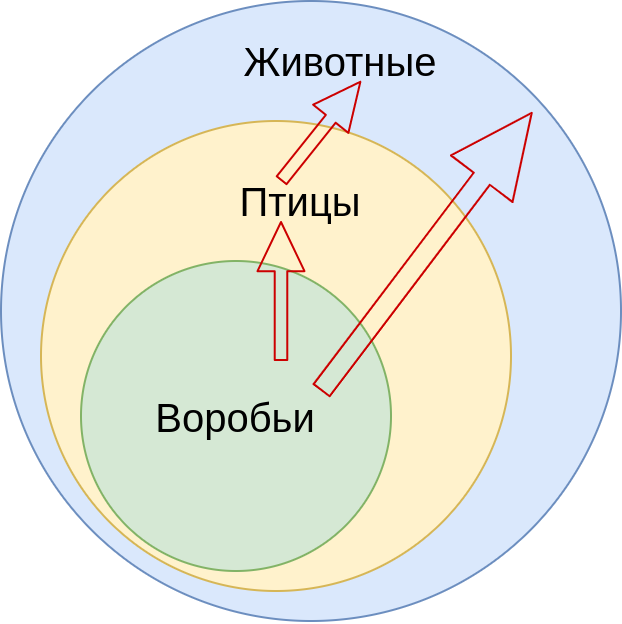
\includegraphics[scale=0.2]{piaf.png}
\end{tabular}
\item При построении суждения посылки могут быть ложными. Более того, в математической логике из ложной посылки следует все, что угодно. Например, \textit{если снег черный, то лес зеленый}. Лес при этом может быть зеленым (летом) и не быть таковым (зимой), но суждение остается истинным, т.к. посылка про снег является ложной.
\item Сравните: если запись числа $a$ оканчивается на 0, то оно кратно 5. Здесь мы ничего не знаем про число $a$, но если для него выполняется посылка, то выполняется и вывод. А если не выполняется, то истинность самого сужджения при этом никак не страдает. Более того, мы знаем, что на 5 также делятся и другие числа, и это значит, что путать местами посылки и вывод ни в коем случае нельзя! Ведь \textbf{не всегда верно}, что если число делится на 5, то его запись заканчивается на 0.
\item Другой~пример:\nopagebreak

\begin{tabular}{lr}
\begin{minipage}[b]{0.5\linewidth}
(\textit{Некоторые французы --- блондины}) и (\textit{некоторые ученики --- французы}), следовательно, (\textit{некоторые ученики --- блондины}). \textbf{Такое суждение неверно}. Поскольку слово <<некоторые>> не гарантирует, что таковым признаком обладают все французы. А значит, из свойства <<быть французом>> не всегда следует <<быть блондином>>.
\end{minipage}& 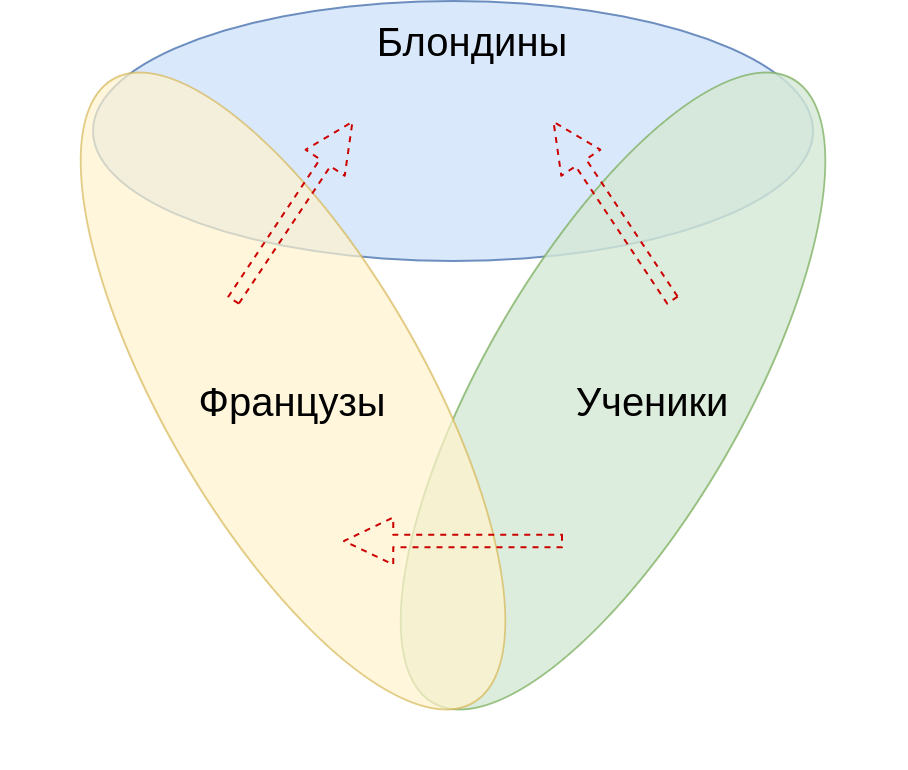
\includegraphics[scale=0.19]{some.png}
\end{tabular}
\item Здесь обе посылки истинные, но вывод ложный. Хотя легко представить ситуацию, когда некоторые ученики действительно будут блондинами. Но это --- лишь предположение, а не строгое рассуждение.
\item В этом примере нарушается именно связка между посылками и выводом, т.к. две посылки не склеиваются по общему признаку. В первой посылке стоит <<некоторые французы>>, а во второй просто <<французы>>, это разные \textbf{множества}, а потому связать две посылки вместе мы не можем!
\item Для построения \textbf{силлогизма} принципиально, чтобы связующее звено было одинаковым:

\begin{center}
\textbf{если} ($A$ есть $B$) и ($B$ есть $C$), \textbf{то} ($A$ есть $C$)
\end{center}
здесь связывание посылок происходит по свойству $B$, и если в нем допустить какое-то искажение, то можно придти к неверным выводам!
\end{enumerate}
\subsection*{Задачи}
\begin{enumerate}
\item Постройте вывод из посылок: (Сократ человек) И (все люди смертны).
\end{enumerate}


\section{Высказывания и предикаты}

\subsection*{Конспект}
\begin{enumerate}\setlength{\itemsep}{1pt}
\item \textbf{Высказывание} --- это любое утверждение на любом языке, которое может быть либо только истинным, либо только ложным.
\item Примеры высказываний: <<\textit{Шесть больше трех}>>, <<\textit{Дважды два --- пять}>>, <<$\sqrt 2$ --- \textit{число иррациональное}>>, <<\textit{среди натуральных чисел существует наибольшее}>>, <<\textit{всякое четное число является суммой двух простых чисел}>>.
\item Все эти высказывания имеют либо истинное, либо ложное значение, хотя про последнее мы не знаем точный ответ. Но мы точно знаем, что их значения не могут быть переменными, т.е. зависеть от каких-то внешних факторов или других высказываний.
\item Из выше приведенных примеров: <<\textit{все птицы --- животные}>> и <<\textit{все воробьи --- птицы}>> есть истинные высказывания.
\item Но эти высказывания можно разобрать на составляющие. Для чего нам понадобятся предикаты.
\item \textbf{Предикат} --- это суждение, зависящее от переменных, обозначающих объекты данного суждения.
\item Например, <<$x$ \textit{есть воробей}>>, <<$x$ \textit{есть птица}>>, <<$x$ \textit{есть животное}>>. Каждое из них может быть истииным или ложным, смотря что подставить вместо $x$. При $x=$ <<\textit{рыба}>> первые два будут ложными, а при $x=$ <<\textit{ромашка}>> ложными будут все три предиката.
\item Аналогично, <<$x$ \textit{есть ученик}>>, <<$x$ \textit{есть француз}>>, <<$x$ \textit{есть блондин}>>. Заметим, что если ранее мы оперировали \textbf{свойствами} (быть учеником, французом, блондином), то теперь перешли к оперированию \textbf{объектом} $x$, который может обладать тем или иным свойством.
\item Из предикатов можно построить новые предикаты, используя логические связки: И($\land$), ИЛИ($\lor$), НЕ($\neg$), СЛЕДУЕТ($\to$).
\item Например, <<($x$ \textit{есть воробей})$\to$($x$ \textit{есть птица}>>), <<($x$ \textit{есть птица})$\to$($x$ \textit{есть животное}>>). Эти предикаты содержат переменную $x$, но они всегда истинны. Такие тождественно истинные предикаты называются \textbf{тавтологиями}. Тавтологии отличаются от истинных высказываний тем, что содержат переменные, которые можно считать фиктивными. Чтобы тавтологию сделать высказыванием, достаточно перед ним сказать <<\textit{для любого} $x$>>, тогда $x$ перестанет быть параметром, а выражение превратится в истинное высказывание:

\begin{center}
<<(\textit{для любого} $x$) ($x$ \textit{есть воробей})$\to$($x$ \textit{есть птица})>>
\end{center}
\item Это называется правилом введения \textbf{квантора всеобщности}.
\item Далее, рассмотрим высказывание <<\textit{некоторые французы блондины}>>. Поступить аналогично предыдущему и заменить его на  предикат <<($x$ \textit{есть француз})$\to$($x$ \textit{есть блондин})>> нельзя! Дело в том, что высказывание <<\textit{все воробьи --- птицы}>> говорит о вложении одного свойства в другое: быть воробьем означает также быть птицей. Но при слове <<\textit{некоторые}>> мы понимаем, что речь идет не о свойстве <<\textit{быть французом}>>, а о том, что некоторые из французов обладают свойством <<\textit{быть блондином}>>. То есть, мы утверждаем, что существует хотя бы один такой объект $x$, который есть и француз и блондин одновременно!
\item Иначе говоря, мы имеем дело со связкой И:
\begin{center}
($x$ \textit{есть француз})$\land$($x$ \textit{есть блондин}),
\end{center}
данный предикат не всегда является истиной, его истинность зависит от конкретного $x$.
\item Тем не менее, и такой предикат можно превратить в высказывание, причем истинное. Для этого нужно слово <<некоторые>> превратить в <<\textit{существует} $x$>>, так что получится истинное высказывание
\begin{center}
<<(\textit{существует} $x$) ($x$ \textit{есть француз})$\land$($x$ \textit{есть блондин})>>
\end{center}
\item Это называется правилом введения \textbf{квантора существования}.
\item Примеры перевода высказываний с языка свойств на язык объектов:\hfill\;

\begin{tabular}{p{0.4\linewidth}p{0.5\linewidth}}\hline
\textit{Все птицы --- животные}  & (\textit{для любого} $x$) ($x$ \textit{есть птица})$\to$($x$ \textit{есть животное}) \\\hline
\textit{Все воробьи --- птицы}  & (\textit{для любого} $x$) ($x$ \textit{есть воробей})$\to$($x$ \textit{есть птица}) \\\hline
\textit{Все воробьи --- животные}  & (\textit{для любого} $x$) ($x$ \textit{есть воробей})$\to$($x$ \textit{есть животное}) \\\hline
Если число заканчивается на 0, то оно кратно 5 &
(\textit{для любого} $a$) ($a$ \textit{заканчивается на $0$})$\to$($a$ \textit{кратно $5$}) \\\hline
Некоторые французы --- блондины 
& (\textit{существует} $x$) ($x$ \textit{есть француз})$\land$($x$ \textit{есть блондин}) \\\hline
Некоторые ученики --- французы 
& (\textit{существует} $x$) ($x$ \textit{есть ученик})$\land$($x$ \textit{есть француз}) \\\hline
Некоторые ученики --- блондины 
& (\textit{существует} $x$) ($x$ \textit{есть ученик})$\land$($x$ \textit{есть блондин}) \\\hline
\end{tabular}

\item Видим, что построить вывод можно только в том случае, когда две посылки склеиваются по общему предикату <<$x$\textit{ есть птица}>>, при этом сами посылки являются импликациями (следование).
\item Можно комбинировать общие и частные суждения:
\begin{center}
<<($x$ \textit{есть птица})$\land$(\textit{все птицы --- животные})>>,
\end{center}
откуда следует вывод <<($x$ \textit{есть животное})>>.

Здесь мы объединили в посылке предикат, что-то говорящий о свойстве объекта $x$, с высказыванием, которое что-то говорит о связи двух свойств, и нашли новое свойство объекта $x$. Это типичное рассуждение от общего к частному.
\item Построение выводов из заданных или полученных ранее истинных высказываний и предикатов называется \textbf{дедукцией} и является основным методом рассуждений при получении математических теорем.
\item Иногда для построения нужного вывода требуетя перебрать сотни комбинаций ранее доказанных посылок. Но часто для нащупывания правильной цепочки доказательства хватает вспомогательных иллюстраций или опыта исследователя, погруженного в данную тему.
\item Ранее мы отмечали, что рассуждения в обратную сторону --- от вывода к посылкам --- неверны. Однако очень часто это верно отчасти. Например, мы знаем дедуктивный вывод: если число оканчивается на 0, то оно делится на 5. На основе этого мы не можем доказать точно, но \textbf{можем предположить}, что если число делится на 5, то оно, вероятно, может оканчиваться на 0. Как мы знаем, это верно примерно в половине случаев. Если бы такое \textit{разворачивание импликации} было бы всегда абсолютно невозможным, то дедукция представляла бы собой простейший случай вывода, когда ложь влечет любое суждение. Для построения теорий это абсолютно бесполезно.
\item Метод \textit{рассуждения назад}, к уже известной посылке, называется \textbf{абдукцией}. Именно таким методом, как правило, пользовался Шерлок Холмс в своих умозаключениях. Именно поэтому его выводы всегда носят вероятностный характер и сопровождаются словами <<вероятно>>, <<скорее всего>> и т.п. Искусство Шерлока Холмса заключается в том, чтобы из всех возможных посылок в данной конкретной ситуации выбрать наиболее вероятную.
\item Например, цитируем из рассказа <<Этюд в багровых тонах>> (Конан Дойль),

\textit{<<Этот человек по типу --- врач, но выправка у него военная. Значит, военный врач. Он только что приехал из тропиков --- лицо у него смуглое, но это не природный оттенок его кожи, так как запястья у него гораздо белее. Лицо изможденное, --- очевидно, немало натерпелся и перенес болезнь. Был ранен в левую руку --- держит ее неподвижно и немножко неестественно. Где же под тропиками военный врач-англичанин мог натерпеться лишений и получить рану? Конечно же, в Афганистане>>. Весь ход мыслей не занял и секунды. И вот я сказал, что вы приехали из Афганистана.}

\item Рассмотрим только часть умозаключений Холмса и сравним их с арифметическим примером\hfill\;

\begin{tabular}{p{0.55\linewidth}p{0.4\linewidth}}\hline
Ватсон --- военный врач с изможденным лицом и загорелый & 
Число 30 --- делится на 5 \\
Воевавшие в Афганистане --- военные с изможденным лицом и загорелые &
Оканчивающее на 0 число --- делится на 5 \\\hline

Вывод: Ватсон прибыл из Афганистана & Вывод: 30 оканчивается на 0\\\hline
\end{tabular}

\item Как видим, нам дано две посылки, в одной из которых дается некая связь между свойствами (воевашие есть военные и т.д., а также оканчивающиеся на 0 делятся на 5), а в другой дается свойство конкретного объекта (Ватсон и число 30). Это свойство общее в обеих посылках, но по нему нельзя склеить их в силлогизм, т.к. свойство всегда стоит в конце посылки. Но Холмс знает, что практически все военные с изможденным лицом и загорелые --- это воевашие в Афганистане (хотя это и неверно на 100\%), и на основании этого он предполагает(!), что и Ватсон такой же, раз он обладает таким же свойством.

\item На примере числа 30 это тоже сработало, однако стоит нам подставить 25 вместо 30, как вся цепочка рассуждений порушится! Поэтому абдуктивные умозаключения нельзя считать математическими, однако они могут навести на правильное дедуктивное умозаключение, в результате чего либо появляется теорема (\textit{Все военные с изможденным лицом воеали в Афганистане}), либо обнаруживается контрпример (в нашем случае это число 25, которое опровергает предположение о том, что все делящиеся на 5 числа оканчаиваются на 0).
\end{enumerate}

\subsection*{Задачи}
\begin{enumerate}
\item Какое абдуктивное предположение можно сделать из следующих посылок: (Зимой выпадает снег) И (Сейчас есть снег) ?
\end{enumerate}


\section{Связь предикатов и множеств}

\subsection*{Конспект}
\begin{enumerate}
\item Выше мы оперировали такими понятиями как свойство и объект, обладающий свойством, на основе чего вводили различные высказывания и предикаты. Посмотрим, как они связаны с понятием \textbf{множество}.
\item Пусть $M$ --- множество всех людей, живущих на планете. Тогда предикат $h(x)$ <<$x$ есть человек>> можно переписать следующим способом: $h(x)=(x\in M)$. Это одновременно означает и то, что $x$ находится в множестве $M$, и то, что $x$ обладает свойством <<быть человеком>>. Говорят также, что $M$ есть область истинности предиката $h(x)$. Таким образом, множество олицетворяет собой свойство, а элементы множества --- объекты, обладающие данным свойством.
\item Если множество $X$ является частью множества $Y$, (например, множество всех женщин есть часть множества $M$), то мы пишем $X\subseteq Y$ ($X$ \textit{содержится в} $Y$, $Y$ \textit{включает} $X$). Важно не путать значки $\in$ и $\subseteq$, т.к. первй говорит о принадлежности объекта к свойству, а второй --- о вложении свойств (о том, что одно свойство меньше или равно другому). Используется также символ строгого вложения $\subset$, означающий, что вложение имеется, но при этом множества не равны.
\item Вложение множеств выражается с помощью принадлежности:
$$
X\subseteq Y\mbox{ эквивалентно }(\forall x) (x\in X)\to(x\in Y)
$$
По сути, это ровно то же самое, что мы ранее делали при переводе языка свойств на язык объектов: \textit{все $X$ есть $Y$} равносильно высказыванию (\textit{для любого} $x$) ($x$ \textit{обладает свойством} $X$)$\to$($x$ \textit{обладает свойством} $Y$).
\item Обозначим далее: $p(x)$ предикат <<$x$ \textit{есть воробей}>>, $o(x)$ предикат <<$x$ \textit{есть птица}>>, $a(x)$ предикат <<$x$ \textit{есть животное}>>. Ранее мы получали следующий вывод:
$$
(\forall x) (p(x)\to o(x))\land (\forall x) (o(x)\to a(x))\vdash(\forall x) (p(x)\to a(x))
$$
\item Попробуем то же самое выразить множествами. Обозначим через $P$ область истинности предиката $p(x)$, т.е. множество всех воробьев, $O$ --- множество всех птиц, $A$ --- множество всех животных. Тогда написанный выше с помощью предикатов вывод можно записать на языке множеств так:
$$
(P\subseteq O\subseteq A) \vdash (P\subseteq A),
$$
поскольку все воробьи есть птицы, все птицы есть животные, а в итоге все воробьи есть животные.
\item На самом деле, существует намного более тесная связь между логическими связками и операциями над множествами.
Вернемся снова к картинке про французов, блондинов и учеников. На ней есть три множества, обозначенные соответствующими овалами. Обозначим их следующим способом:
$$
F = \{x\mid x\mbox{ --- француз}\},\quad B = \{x\mid x\mbox{ --- блондин}\},\quad E = \{x\mid x\mbox{ --- ученик}\}
$$
\item Здесь можно увидеть примеры \textbf{пересечений} множеств:
\begin{gather*}
F\cap B = \{x\mid (x\mbox{ --- француз})\land (x\mbox{ --- блондин})\},\\
F\cap E = \{x\mid (x\mbox{ --- француз})\land (x\mbox{ --- ученик})\},\\
E\cap B = \{x\mid (x\mbox{ --- ученик})\land (x\mbox{ --- блондин})\}.
\end{gather*}
Видим, что они соответствуют логической связке И соответствующих предикатов, выражающих свойства.
\item На той же схеме мы можем усмотреть и такие теоретико-множественные конструкции, как:
$$
F\setminus B = \{x\mid (x\mbox{ --- француз})\land \neg(x\mbox{ --- блондин})\},
$$
т.е. множество французов, не являющихся блондинами. $F\setminus B$ есть операция \textbf{вычитания} множеств.
\item Наконец, множество 
$$
F\cup E  = \{x\mid (x\mbox{ --- француз})\lor (x\mbox{ --- ученик})\}
$$
представляет собой свойство быть французом ИЛИ учеником. Оно содержит в себе как всех французов, так и всех учеников, причем среди них есть как французы, не являющиеся учениками, так и французы, являющиеся уничениками, а также ученики, не являющиеся французами. \textbf{Объединение} множеств соответствует логической связке ИЛИ.
\item Итак, мы можем легко оперировать предикатами, представляя, что они выражают свойство объекта принадлежать некоторому множеству, и наоборот, оперировать множествами, представляя, что оперируем предикатами, для которых эти множества суть область истинности. При этом И соответствует пересечению, ИЛИ --- обединению множеств. Отрицание соответствует вычитанию множеств, причем разность $X\setminus Y$ можно рассматривать как пересечение $X\cap(\neg Y)$. Наконец, вложение множеств соответствует импликации предикатов.
\end{enumerate}



\subsection*{Задачи}
\begin{enumerate}
\item Выразить свойство <<\textit{быть учеником и блондином одновременно}>> через множества $E$ и $B$.
\item Написать множество, соответствующее всем <<\textit{птицам, не являющимся воробьями}>> через множества $O$ и $P$.
\item Какие элементы содержит множество $P\setminus A$, множество $M\cap F$, множество $(F\cup B)\setminus (F\cap B)$?
\item Что выражает высказывание $(M\setminus F)\subseteq (M\setminus B)$?
\item Докажите: $(E\subseteq F)\vdash (M\setminus F)\subseteq (M\setminus E)$ (от противного).
\end{enumerate}


\section{Построение множеств}

\subsection*{Конспект}
\begin{enumerate}
\item Построение множеств прямо наследует из их связи с предикатами. Тем не менее, важно знать язык, позволяющмй компактно и наглядно записывать конструктивные примеры построения множеств.
\item Конечное множество, элементами которого являются объекты $a,b,\dots,z$ (их не обязательно 26, просто какой-то набор), обозначается
$$
\{a,b,\dots,z\},
$$
при этом неважно, в каком порядке записаны элементы внутри скобок, и есть ли там дубликаты. Если в списке один и тот же элемент повторяется несколько раз, то его дубли можно спокойно выбрасывать.\footnote{В математике существует понятие \textbf{мультимножество}, в котором как раз количество дубликатов имеет значение и называется кратностью элемента. Мультимножество удобно, например, для записи разложения числа по степеням простых.}
\item Примеры: $\{0\}$, $\{0,1\}$, $\{0,1,2,3\}$, $\{0,0,1,1,1\}$. Последнее множество равно множеству $\{0,1\}$ (убрали кратные вхождения). Еще пример: $\{\}$ --- \textbf{пустое множество}, обозначаемое также символом $\emptyset$.
\item Как мы уже видели ранее, множество можно задать в \textbf{предикативной форме}, общий вид которой такой:
$$
\{x\mid \ph(x)\},\quad \{f(x)\mid \ph(x)\},
$$
где $\ph(x)$ --- это предикат, выражающий свойство объекта $x$, а $f(x)$ --- некоторое преобразование объекта $x$ (функция). 

В первом случае даное множество является областью истинности предиката $\ph(x)$ и содержит в себе все элементы, и только их, для которых $\ph(x)$ истинно. Во втором случае множество содержит все значения функции $f(x)$, примененные к объектам из области истинности $\ph(x)$. Очевидно, что
$$
\{f(x)\mid \ph(x)\} = \{y\mid(y=f(x))\land\ph(x)\}
$$

\item Конечное множество в предикативной форме записывается так:
$$
\{a,b,\dots,z\} = \{x\mid (x=a)\lor(x=b)\lor\dots\lor(x=z)\},
$$
где предикат $\ph(x)=(x=a)\lor(x=b)\lor\dots\lor(x=z)$ выражает свойство $x$ входить в список объектов $a,b,\dots,z$.
\item Объединение (или сумма) множеств:
$$
A\cup B = \{x\mid (x\in A)\lor(x\in B)\},
$$
например, $\{a,b\}\cup\{b,c\}=\{a,b,c\}$.
\item Пересечение множеств:
$$
A\cap B = \{x\mid (x\in A)\land(x\in B)\},
$$
например, $\{a,b\}\cup\{b,c\}=\{b\}$.
\item Разность множеств:
$$
A\setminus B = \{x\mid (x\in A)\land(x\notin B)\},
$$
например, $\{a,b\}\setminus\{b,c\}=\{a\}$. Заметим, что $A\setminus B$ не всегда равно $B\setminus A$.
\item Если элементы множеств --- это числа, то с ними можно производить арифметические операции:
$$
A+B = \{x+y\mid (x\in A)\land(y\in B)\}, \quad kA = \{kx\mid x\in A\},
$$
здесь первое множество --- это сумма по Минковскому двух множеств, оно содержит все возможные суммы $x+y$, где первое слагаемое берется из первого множества, второе --- из второго.

Легко видеть также, что $A+\emptyset=\emptyset$, т.к. предикат $y\in B$ в случае $B=\emptyset$ тождественно ложный.

\textbf{Важно}: не следует путать $A+A$ и $2A$! Например,
$$
\{0,1\}+\{0,1\}=\{0,1,2\},\mbox{ но }2\{0,1\}=\{0,2\}.
$$

\item Аналогично можно определить произведение множеств по Минковскому:
$$
AB = \{xy\mid (x\in A)\land(y\in B)\},
$$
откуда легко определяется степень множества $A^k$, а также его экспонента $\exp(A)=\sum_k(1/k!)A^k$.

Аналогично сумме видим, что $A\emptyset=\emptyset$.
\end{enumerate}





\subsection*{Задачи}
\begin{enumerate}
\item Найти объединение, пересечение и разность множеств $\{0,1,2,3\}$ и $\{1,2,5\}$ (разность как в прямом, так и в обратном порядке).
\item Записать множество $\{0,1,2\}$ в предикативной форме.
\item Записать множество всех простых чисел в предикативной форме.
\item Доказать, что $A+\{0\}=A$, $A\cdot\{1\}=A$.
\item ${}^{**}$Когда $A\setminus B=B\setminus A$?
\item ${}^{***}$Доказать, что $\max\exp(\{0,x\}) = e^x$.
\end{enumerate}


\end{comment}



\begin{comment}
\chapter{1. Визуальная арифметика}
\end{comment}
\newchapter{Визуальная арифметика}

\vrezka{В данной главе закладывается фундамент арифметики с помощью визуальных образов. Действия с отрезками и прямоугольниками являются иллюстрацией действий с числами. Цель --- дать наглядное обоснование законам арифметики и получить некоторые навыки арифметических операций и сравнений чисел.

Попутно вводится понятие натурального числа как количества применяемых операций композиции, а также как меры длины, площади, объема относительно заданной мерной единицы.
}


\section{Запись действий с отрезками}

\lesson{Учимся складывать и вычитать наглядно, используя отрезки и складную линейку}


\begin{enumerate}\setlength{\itemsep}{1pt}
\item Берем произвольную прямую, и на ней будем откладывать отрезки --- вправо и влево.
\item Откладывание вправо есть прибавление длины, а откладывание влево --- вычитание (уменьшение) длины.
\item Можно откладывать ноль, т.е. ничего не делать. В этом случае все равно --- прибавляем или вычитаем ноль.
\item Мы можем комбинировать откладывание отрезков вправо и влево, т.е. производить серию последовательных откладываний отрезков (они могут быть разными по длине), на каждом шаге --- от текущей точки приложения.
\item Результат \textit{серии откладываний} равносилен одному откладыванию отрезка, соединяющего стартовую и финишную точки, причем финишная точка:
\begin{itemize}
\item может быть справа от стартовой (результатом является одно откладывание вправо, т.е. прибавление длины),
\item может совпадать с ней (результатом оказалось нулевое откладывание)
\item или быть слева от стартовой точки (результатом является одно откладывание влево, т.е. вычитание).
\end{itemize}
\item Откладывание \textit{изотропно}, т.е. одинаковые серии откладываний, приложенные к разным стартовым точкам, приводят к одинаковым результирующим отрезкам, отложенным от этих стартовых точек. Иначе говоря, величина и направление откладывания не зависит от начального местоположения!
\end{enumerate}
\begin{tabular}{ll}
\begin{minipage}{0.6\linewidth}
\begin{enumerate}\setcounter{enumi}{6}
\item Серии откладываний можно проиллюстрировать складным метром. Раскладывание колена на $180^o$ означает прибавление его длины к общей серии откладываний, а складывание --- вычитание его длины из общей серии откладываний. При этом от стартовой точки можно уйти как вправо, так и влево, или остаться на месте.
\end{enumerate}
\end{minipage}
&
\begin{minipage}{0.4\linewidth}
%\begin{figure}[h]%[htb!]
%\vspace*{3mm}
%\begin{center}
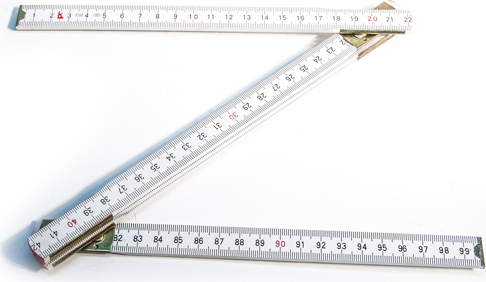
\includegraphics[scale=0.3]{meter.png}
%\end{center}
%\label{meter}
%\end{figure}
\end{minipage}
\end{tabular}
\begin{enumerate}\setcounter{enumi}{7}
\item С помощью этой же линейки нетрудно продемонстрировать, что композиция откладываний
\begin{itemize}
\item \textbf{ассоциативна}, т.е. одни и те же манипуляции с линейкой мы можем производить в разном порядке, например, сначала разложить два ее начальных колена, а затем разложить два колена в конце, и это будет ровно то же самое, как в случае раскладывания сначала конечного участка, а затем начального --- финальная конфигурация линейки будет одинаковой;
\item \textbf{коммутативна}, т.е. можно взять две линейки, произвести над ними какие-то манипуляции по складыванию/раскладыванию, затем их состыковать, и результат (направление и число колен линейки от начальной точки до конечной) не будет зависеть от того, в каком порядке линейки будут состыкованы.
\end{itemize}
\item Кроме того, очевидно, что у каждого откладывания существует обратное, приводящее в результате к нулевому откладыванию. Для этого нужно произвести ровно ту же самую серию откладываний, только поменять направление. Или, что то же самое, пройти по линейке в обратную сторону.
\item Далее любое откладывание будем записывать буквами $a,b,c,\dots$, имея ввиду под ними как прибавления, так и вычитания.
\item Откладывание, противоположное $a$, будем обозначать $-a$. При этом комбинация откладываний соединяется знаком '+', а если встречается комбинация $a+(-b)$, то пишем проще: $a-b$.
\item Обратные откладывания --- это просто перевернутые в обратную сторону <<линейки>>!
\item Результат откладывания (конфигурацию линейки с учтом ее направления) будем называть \textbf{вектором}. Если вектор смотрит влево (финишная точка левее стартовой), то вектор называется \textit{отрицательным}, а если вправо --- \textit{положительным}. Нулевой вектор --- когда финиш и старт совпадают.
\item Композицию откладываний будем называть \textbf{суммой векторов} или просто суммой, а процедуру откладывания --- \textbf{сложением}.
\end{enumerate}

\textbf{Свойства сложения}:
\begin{enumerate}[label=S\arabic*]
\item $(a+b)+c=a+(b+c)$ (ассоциативность).\index{Ассоциативность}
\item $a+b=b+a$ (коммутативность).\index{Коммутативность}
\item $a+0=0+a=a$ (аддитивное свойство нуля).\index{Нейтральный элемент}

Первые 3 свойства выше уже были продемонстрированы в процессе определения операций с линейкой. Добавим, что откладывания линейки еще можно рассматривать как путь некоего одномерного путешественника, который идет по прямой линии то вправо, то влево. Если он идет вправо, то прибавляет шаги, а если влево, то вычитает, т.е. делает обратный отсчет. Нулевой путь означает, что он прошел в одну сторону столько же, сколько в другую.

\item $a+(-a)=0$ (обратный элемент).\index{Обратный элемент}

Здесь помогает та же иллюстрация с путешественником. Он прошел сначала вправо $a$ шагов, затем влево столько же. В итоге пришел в начало пути, а это и означает по определению, что он прошел нулевой путь.

Конечно, с точки зрения физики он прошел в два раза больше, чем в одну сторону, но нас в данном случае интересует не то, сколько он потратил времени или сил на проделанный маршрут, а то, в какой точке линейки он оказался в финале. Для измерения его физических потерь нам потребуется ввести понятие пути и его длины. Но это мы отложим до более глубоких изысканий.

\item Если $a+x=b+x$, то $a=b$ (правило сокращения).

Добавим к исходному равенству в обоих частях элемент $-x$, обратный к $x$, и получим
$$
(a+x)+(-x) = a+(x+(-x)) = a,
$$
где мы воспользовались ассоциативностью операции сложения. Аналогично заключаем, что $(b+x)+(-x) = b+(x+(-x)) = b$. Таким образом, $a=b$.

\item Верно одно и только одно: либо $a=b$, либо $a=b+x$, либо $a=b-x$, где $x$ --- откладывание вправо (трихотомия).

Это утверждение также требует наглядного интуитивного доказательства. Тут нужно понимать, что наша линейка представляет собой один связный отрезок, а значит, путешественник может пройти по ней из любой точки в любую точку. Отметим на ней две точки $a$ и $b$. Если $a$ находится левее $b$, то нужно пройти положительный путь от $a$ к $b$, это и есть наше $x$, а если наоборот, то отрицательный, т.е. $-x$.
\end{enumerate}

\begin{enumerate}\setcounter{enumi}{14}
\item Понятие отрицательного и положительного векторов позволяют ввести сравнение на векторах.
\item Для начала скажем, что положительный вектор больше нуля: $x>0$.
\item Далее, если $b=a+x$, где $x>0$, то пишем $a<b$.
\item \textbf{Свойства сравнения} (очевидны):
\begin{enumerate}[label=O\arabic*]
\item не верно, что $x<x$ (антирефлексивность);
\item если $a<b$ и $b<c$, то $a<c$ (транзитивность);
\item верно одно и только одно: либо $a=b$, либо $a<b$, либо $b<a$ (трихотомия);
\item $a<b\Leftrightarrow a+x<b+x$, где $x>0$ (изотропность сравнения)
\end{enumerate}

\end{enumerate}


\lesson{Визуализация умножения через площадь и объем}


\begin{enumerate}
\item Строим две перпендикулярно направленные оси $Ox$ и $Oy$. На каждой оси --- свой собственный мир векторов и линеек.
\item Умножение --- это площадь, построенная на перпендикулярных векторах. Картинка $5\times 3=15$ (см. рис. \ref{prod}).
\begin{figure}[hbt!]
\begin{center}
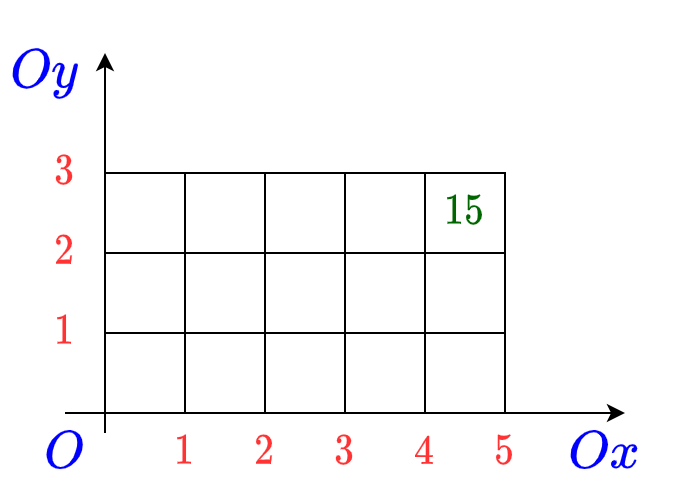
\includegraphics[scale=0.2]{prod.png}
\end{center}
\caption{}\label{prod}
\end{figure}
\item Площадь --- величина всегда положительная, а векторы мы умеем откладывать вверх и вниз, вправо и влево, т.к. имеем две перпендикулярные линейки. Соответственно, у нас имеется 4 различных ситуации: вправо и вверх, вправо и вниз, влево и вверх, влево и вниз.

Здесь мы впервые сталкиваемся с таким понятием, как \textit{ориентированная площадь}. Представим себе, что в нашу плоскость воткнута перпендикулярная ось, с конца которой мы наблюдаем за откладыванием векторов и подсчетом площадей. Когда первый вектор отложен вправо, а второй вверх, то площадь прямоугольника, наблюдаемая нами сверху, заметается по направлению от первого вектора ко второму. Такое направление (против часовой стрелки, или от оси $Ox$ к оси $Oy$) в математике принято считать положительным направлением. Поэтому соответствующую площадь мы считаем положительной.\footnote{То, что именно такое направление следует называть положительным, --- это всего лишь вопрос договоренностей о теримнах.}

\begin{figure}[hbt!]
\begin{center}
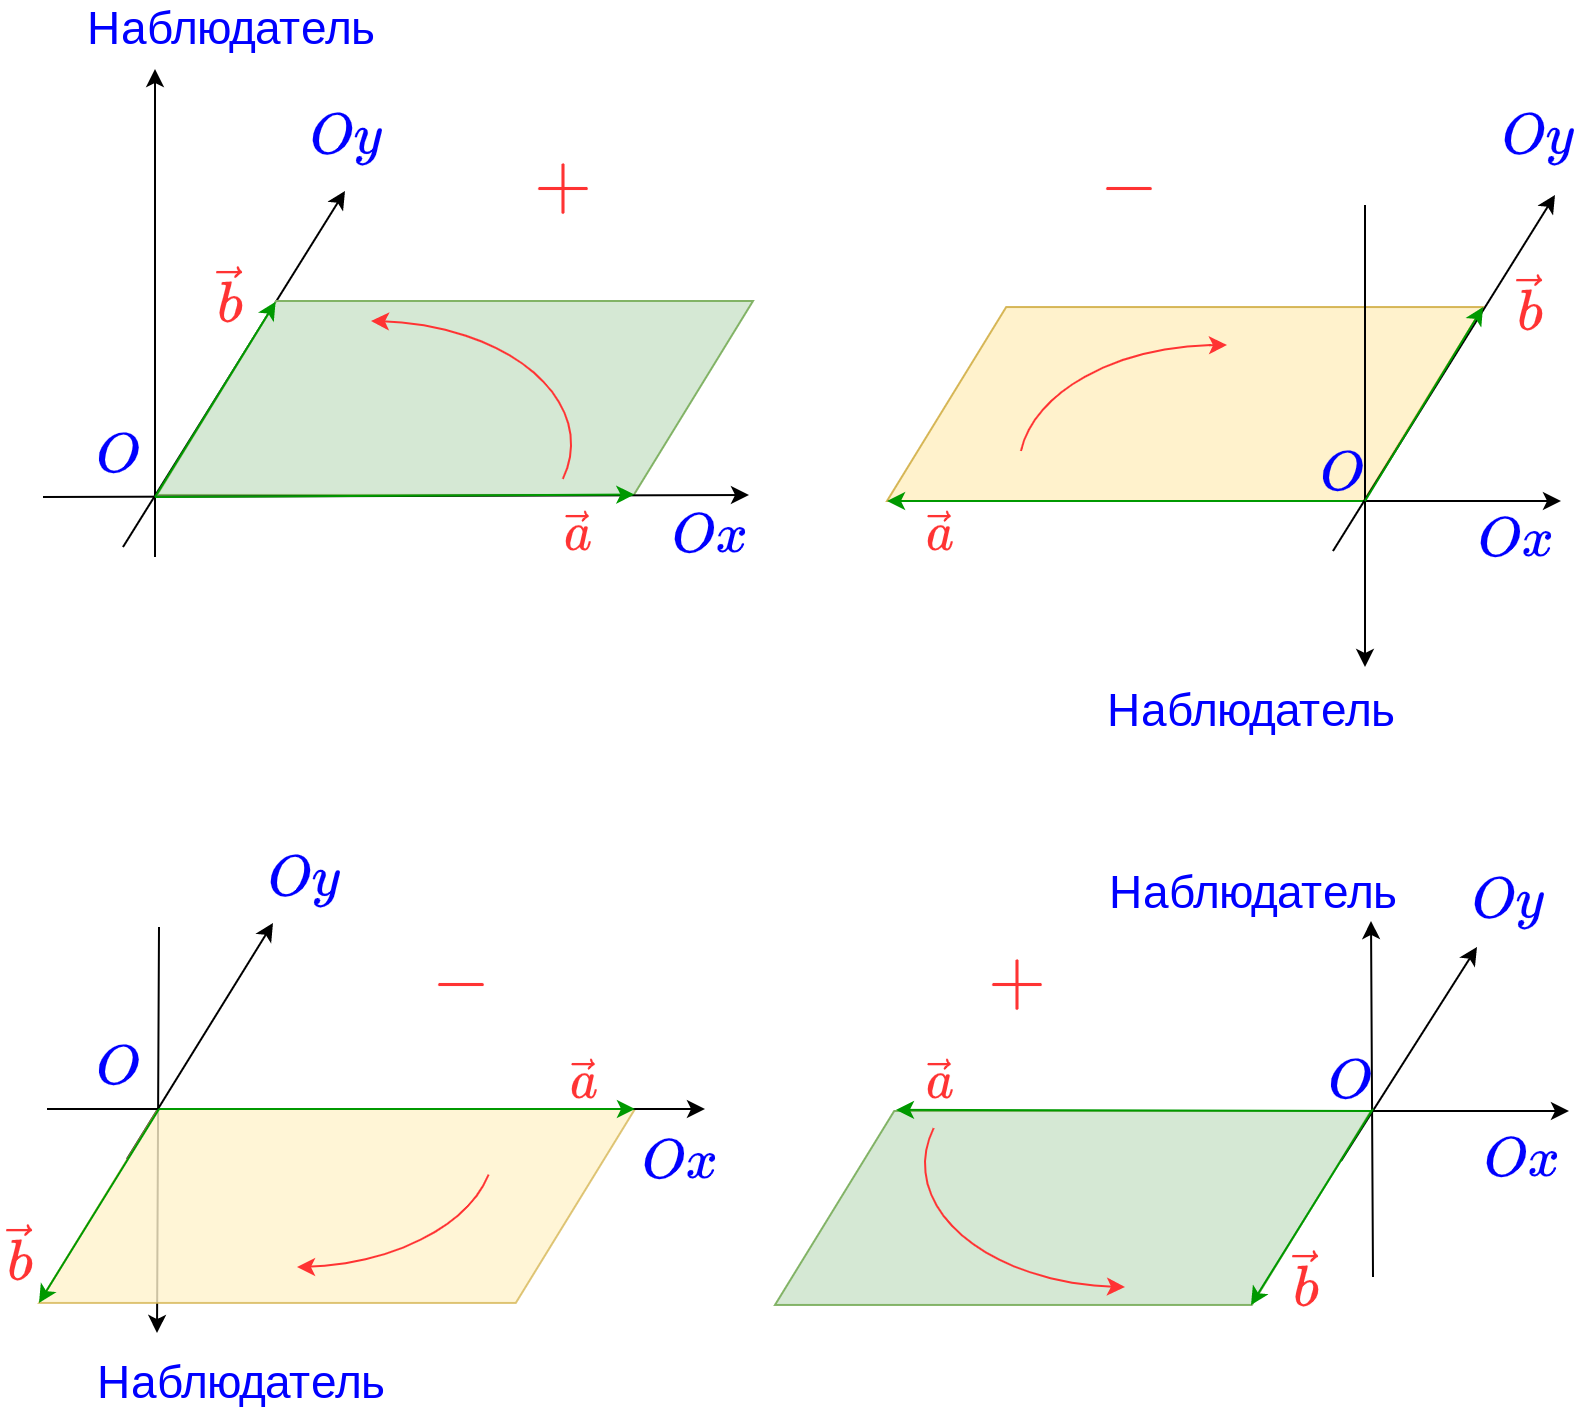
\includegraphics[scale=0.2]{mult.png}
\end{center}
\caption{}\label{mult}
\end{figure}

Теперь перевернем правый вектор, лежащий на оси $Ox$ и смотрящий вправо, через начало координат, в результате чего он будет смотреть влево и станет отрицательным. Вместе с ним перевернется и наш прямоугольник, площадь которого мы наблюдаем. И вместе с ним перевернется и наблюдательная вышка. Ее направление станет противоположным. И хотя мы по-прежнему с ее конца будем наблюдать площадь в правильном направлении, вся конструкция перевернется и сменит ориентацию в пространстве на противоположную, поэтому произведение отрицательного вектора на положительный станет также отрицательным.

Далее мы перекинем вектор, лежащий на оси $Oy$ через начало координат, так что он станет смотреть вниз, и прямоугольник. построенный на этих векторах, снова окажется в правильном, положительном положении, хотя обе его стороны есть отрицатлеьные числа. Стало быть, произведение двух отрицателных чисел есть число положительное.

Наконец, еще одна манипуляция с вектором $Ox$ в обратную сторону снова переведет конструкцию в отрицательное положение, и произведение снова станет отрицательным.

Итак, мы видим, что как только мы снабжаем плоскость дополнительным пространственным ориентиром, мы можем различать знак площади, сделать ее ориентированной в зависимости от того, куда направлены векторы, порождающие данную площадь.

В дальнейшем мы столкнемся с еще болеее общей конструкцией, где будем строить ориентированную площадь на произвольном параллелограмме. Но и там ситуация распадется на два знаковых класса в зависимости от ориентации векторов.

Таким образом, знак умножения двух чисел (площадь) определяется знаком (направлением) векторов и таблицей композиции знаков:
\begin{center}
\begin{tabular}{c|c|c|}
  & $+$ & $-$ \\
 \hline
$+$ & $+$ & $-$ \\
 \hline
$-$ & $-$ & $+$ \\
\hline
\end{tabular}
\end{center}
\item Данная таблица демонстрирует нам простейший пример группы. Во-первых, мы видим здесь, что композиция знаков тоже есть знак, во-вторых, что композиция любого знака с плюсом ничего не меняет, т.е. плюс является нейтральным в операции композиции. В-третьих, что знак минус сам себе обратен, так как умножение его самого на себя дает плюс. Все эти свойства являются определяющими свойствами математического понятия группы, и будут <<работать>> на потяжении всгео курса.


\item Отметим, что умножение можно иллюстрировать не только площадью, но и объемом, если нам необходимо перемножить три числа. Хотя сама по себе операция умножения бинарная (т.е. имеет два аргумента), один из множителей, в свою очередь, также может быть результатом операции умножения, так что в итоге получается умножение трех чисел. Более того, любое число $a$ можно представить как площадь прямоугольника $a\times 1$. И наоборот, произведение $a\times b$ можно вытянуть в линию из $ab$ квадратиков, тем самым перейдя от площали к отрезку. Поэтому в дальнейшем умножение векторов в смысле нахождения площади/объема, т.е. $a\times b$, и умножение чисел как таковых, т.е. $ab$, будем считать одним и тем же понятием и обозначать одинаково, так что $a\times b=ab$.

\item \textit{Степень}: многократное умножение отрезка самого на себя. Поскольку степень есть частный случай многократного умножения, то вотрая степень, очевидно, представляется площадью квадрата, третья --- куба, а для иллюстрации более высоких степеней потребуются и более высокие размерности.
\end{enumerate}


\textbf{Свойства умножения}:
\begin{enumerate}[label=P\arabic*]
\item $(a\times b)\times c = a\times (b\times c)$ (ассоциативность --- рис. \ref{assoc});\index{Ассоциативность}

\begin{figure}[hbt!]
\begin{center}
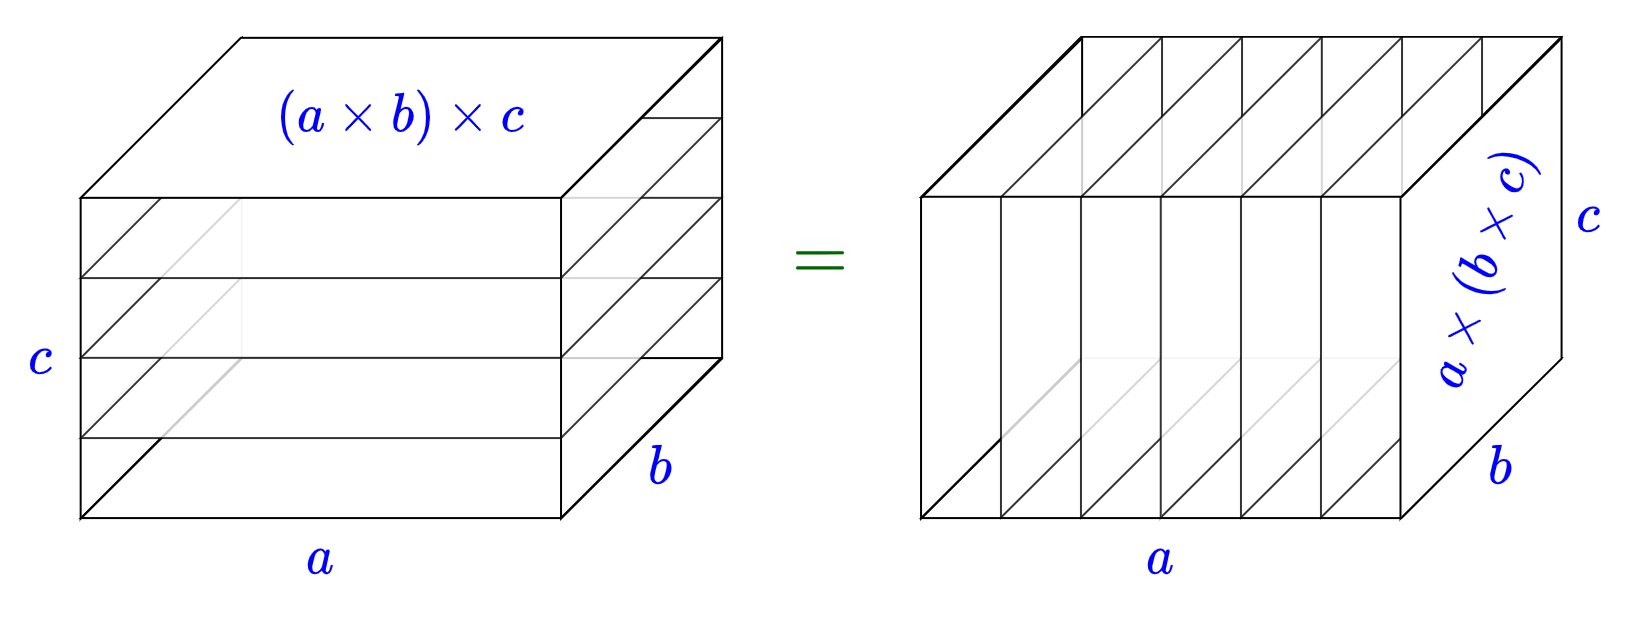
\includegraphics[scale=0.2]{assoc.png}
\end{center}
\caption{}\label{assoc}
\end{figure}

\item $a\times b=b\times a$ (коммутативность --- рис. \ref{kommut});\index{Коммутативность}

\begin{figure}[hbt!]
\begin{center}
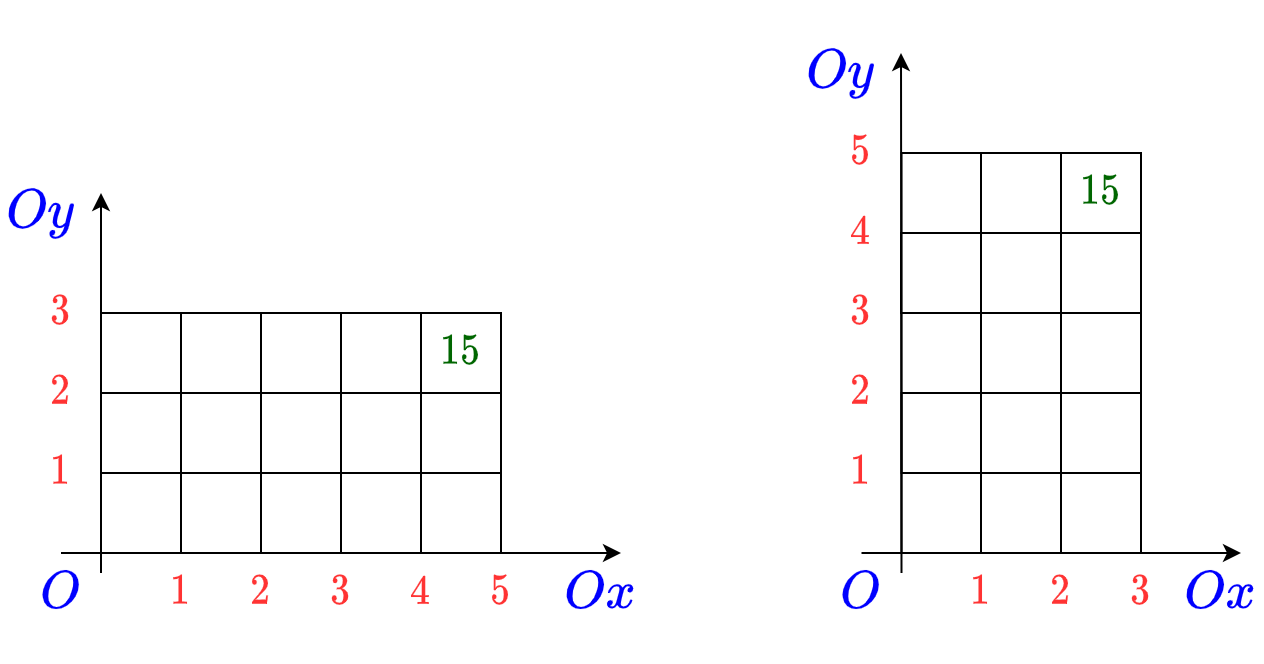
\includegraphics[scale=0.2]{kommut.png}
\end{center}
\caption{}\label{kommut}
\end{figure}

\item $a\times 1=1\times a=a$ (нейтральный элемент по умножению);\index{Нейтральный элемент}

\item $a\times(b+c)=a\times b+a\times c$ (дистрибутивный закон --- рис. \ref{distr});\index{Дистрибутивность}

\begin{figure}[hbt!]
\begin{center}
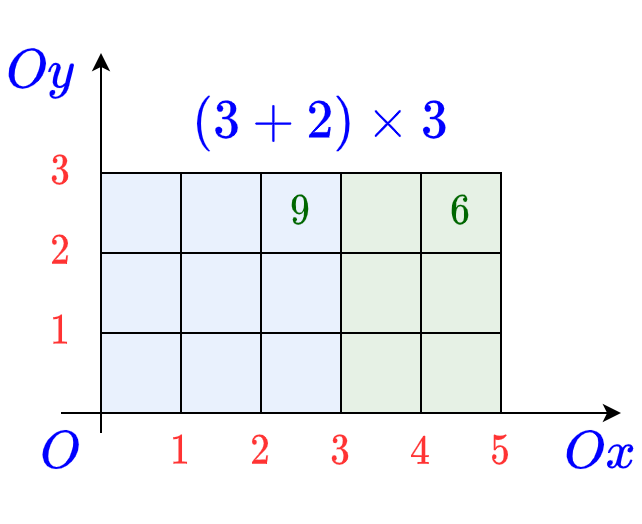
\includegraphics[scale=0.2]{distr.png}
\end{center}
\caption{}\label{distr}
\end{figure}

\item Умножение на нулевой отрезок (мультипликативное свойство нуля) --- применим свойство сложения с нулем, дистрибутивность и сокращение на одинаковое слагаемое:\index{Мультипликативное свойство нуля}
$$
0 + a\times 0 = a\times 0 = a\times (0+0) = (a\times 0) + (a\times 0)\Rightarrow 0 = (a\times 0).
$$

\item если $a\times b=0$, то $a=0$ или $b=0$ (отсутствие делителей нуля);\index{Делители нуля}

Предполагая, что $a\ne0\ne b$, построим прямоугольник $a\times b$, он точно будет ненулевой площади --- см. рис. \ref{prod}.

\item если $a\times c=b\times c$ и $c\ne 0$, то $a=b$ (правило сокращения);

Найдем разность и воспользуемся дистрибутивностью:
$$
0 = a\times c-b\times c = (a-b)\times c,
$$
а так как $c\ne 0$, получаем, что $a-b=0$, т.е. $a=b$.

\item если $a<b$ и $c>0$, то $a\times c<b\times c$, и обратно: если $a\times c<b\times c$ и $c>0$, то $a<b$ (монотонность --- рис. \ref{monot});

\begin{figure}[hbt!]
\begin{center}
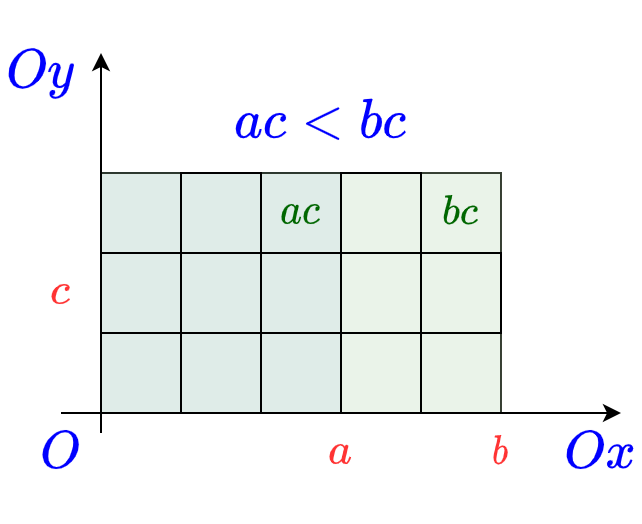
\includegraphics[scale=0.2]{monot.png}
\end{center}
\caption{}\label{monot}
\end{figure}

\end{enumerate}


\subsection*{Задачи}
\begin{enumerate}
\item Нанести метки на прямой, соответствующие шагам вправо и влево, считая начальной точкой $O$, а все шаги равновеликими. Дойти до точки 10 и -10.
\item Описать в терминах одномерного путешественника операции сложения: $5+3$, $8-4$, $3-5$, $-2-6$.
\end{enumerate}



\section{Понятие натурального числа}

\lesson{Натуральные числа как кратность операций сложения и умножения. Понятие делимости/кратности. Ноль кратен любому числу}

\begin{enumerate}
\item Ранее мы вводили определение степени числа как многократного применения операции умножения на одно и то же число. Ясно, что то же самое можно определить и в отношении многократной операции сложения одного и того же числа с самим собой. Только в случае сложения <<степень>> есть обычное умножение. Действительно, многократное сложение $a+a+a+a+a+\dots$, если воспользоваться графическим представлением, есть просто умножение отрезка $a$ на отрезок длины $1+1+1+\dots$, где единицы взяты ровно в том же количестве, в каком встречается $a$ (рис. \ref{kratplus}).

\begin{figure}[hbt!]
\begin{center}
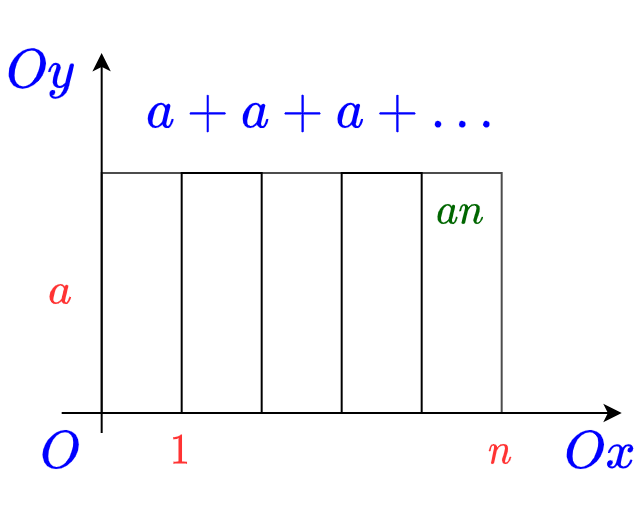
\includegraphics[scale=0.2]{kratplus.png}
\end{center}
\caption{}\label{kratplus}
\end{figure}

В итоге, если мы число $a$ складываем $n$ раз (где $n$ --- это обозначение суммы единиц), то это все равно, что мы производим умножение
$$
a\times(\underbrace{1+1+\dots+1}_{n}).
$$

В случае многократного умножения действуем по аналогии:  $a a a\ldots$ обозначаем как $a^n$, понимая под $n$ количество чисел $a$, которые мы перемножили.

Вот эта количественная роль чисел, которые выступают для обозначения кратности однотипных операций, и является смыслом натурального числа. Натуральное число есть ответ на вопрос <<сколько раз?>> или <<сколько штук?>>

Целые числа не могут похвастаться таким натуральным (предметным) определением. В целых числах к количеству добавляется еще и направление (назад или вперед, но об этом --- позже), а рациональное число отражает отношение между количествами.

\item Нулевая кратность: в случае сложения ничего не складываем, остаемся на месте в начальной точке, поэтому
$$
\underbrace{a+\dots+a}_{0\mbox{ раз}}=0.
$$
\item Нулевая степень: в случае умножения ничего не умножаем, от умножения остается только 1:
$$
\underbrace{a\times\dots\times a}_{0\mbox{ раз}}=1.
$$
Почему именно 1? Потому что если мы начнем перемножать разные числа с разными кратностями
$$
\underbrace{aa}_{?}\underbrace{bbbb}_{?}\underbrace{ccccc}_{?},
$$
то результат не должен меняться, если кратность одной из переменных станет равной нулю. В данном примере любую из кратностей можно сделать нулевой, тогда эта переменная выпадет из записи, и результат останется верным, только если нулевая кратность умножения равна 1.

Многие правила в математике для крайних значений определяются с целью сохранить общий вид формул, если это не приводит к противоречию.
\item Итак, \textbf{натуральные числа}\index{Числа!натуральные}\index{Натуральные числа} --- это показатели кратности операций (сложения и умножения).
\item С другой стороны, ничто не мешает нам сумму единиц рассматривать саму по себе, т.е. как сумму единичных отрезков. В данном случае нет никакой разницы между суммой единичных отрезков и кратностью сложения единичного отрезка.
\item Такая интерпретация натурального числа вполне согласуется с операциями сложения и умножения, сохраняет все законы арифметики: ассоциативность, коммутативность, дистрибутивность.
\item Поэтому натуральные числа, привязанные к единичным отрезкам, можно также считать мерой длины, площади, объема и т.д.
\item Ноль мы будем считать натуральным числом, поскольку мы рассматриваем нулевую кратность для однородности законов арифметики.
\item[\bf NB] Натуральные числа --- это и кратности операций, и единицы измерения, т.е. числа.
\item Натуральные числа отвечают за соизмеримость и арифметическую кратность чисел (любых): $a$ \textbf{кратно}\index{Кратность чисел} $b$ ($a\mathop{\vdots} b$), если $a=bn$ или $a=(-b)n$ при некотором натуральном $n$. Ноль кратен любому числу! Нулю кратен только ноль!

Действительно, $0\mathop{\vdots} b$ означает, что при некотором $n$ имеем $0=bn$. Это верно как раз при $n=0$. Предположим, что какое-то число кратно нулю: $a\mathop{\vdots} 0$, тогда при некотором $n$ должно быть $a=0n$. Но при любом $n$ имеем $0n=0$, так что только $a=0$ будет кратно нулю.

\item Если $a$ кратно $b$, то говорят также, что $b$ \textbf{делит} $a$, или что $b$ является делителем $a$ ($b|a$).\index{Делимость чисел}
\item Если $a>0$ кратно $b>0$, то $a=kb=b+(k-1)b$, где $k>0$. Здесь $x=(k-1)b$. Поэтому $a\ge b$. Так что для положительных векторов кратность означает превосходство в смысле сравнения. Аналогичные неравенства можно получить и для отрицательных векторов.
\end{enumerate}
\subsection*{Задачи}
\begin{enumerate}
\item Доказать, что если $a|b$ и $b|c$, то $a|c$.
\item Доказать, что если $a|b$ и $b|a$, то $a=\pm b$ ($a,b$ --- произвольные векторы).
\end{enumerate}


\section{Визуальные доказательства}\label{vizual}

\lesson{Теорема Пифагора геометрически. Бином Ньютона разрезанием кубика}
\href{https://www.youtube.com/watch?v=Xdc8WWFURA8}{Видеоурок про теорему Пифагора}

\href{https://www.youtube.com/watch?v=YXYQmxLDtMw}{Видеоурок про бином Ньютона}

\begin{enumerate}
\item \textbf{Квадрат суммы}. Строим квадрат $(a+b)\times (a+b)$ и внутри него квадраты $a\times a$ и $b\times b$ (см. рис. \ref{pithagor}). Приравнивая площадь всего квадрата к сумме его частей, получаем, что
$$
(a+b)^2 = a^2 + 2ab + b^2.
$$
\item \textbf{Теорема Пифагора}. Далее, строим еще один квдарат $(a+b)\times (a+b)$ и внутри квадрат $c\times c$, где $c$ --- это гипотенуза треугольника с катетами $a$ и $b$ (рис. \ref{pithagor}). Далее заштрихуем одинаковые треугольники в левом и правом квадратах. А поскольку оба больших квадрата равны, равны и их площади, а также площади тех остатков, которые получается, если выбросить заштрихованные треугольники. То, что остается, дает равенство:
$$
a^2+b^2=c^2,
$$
т.е. теорему Пифагора.

\begin{figure}[hbt!]
\begin{center}
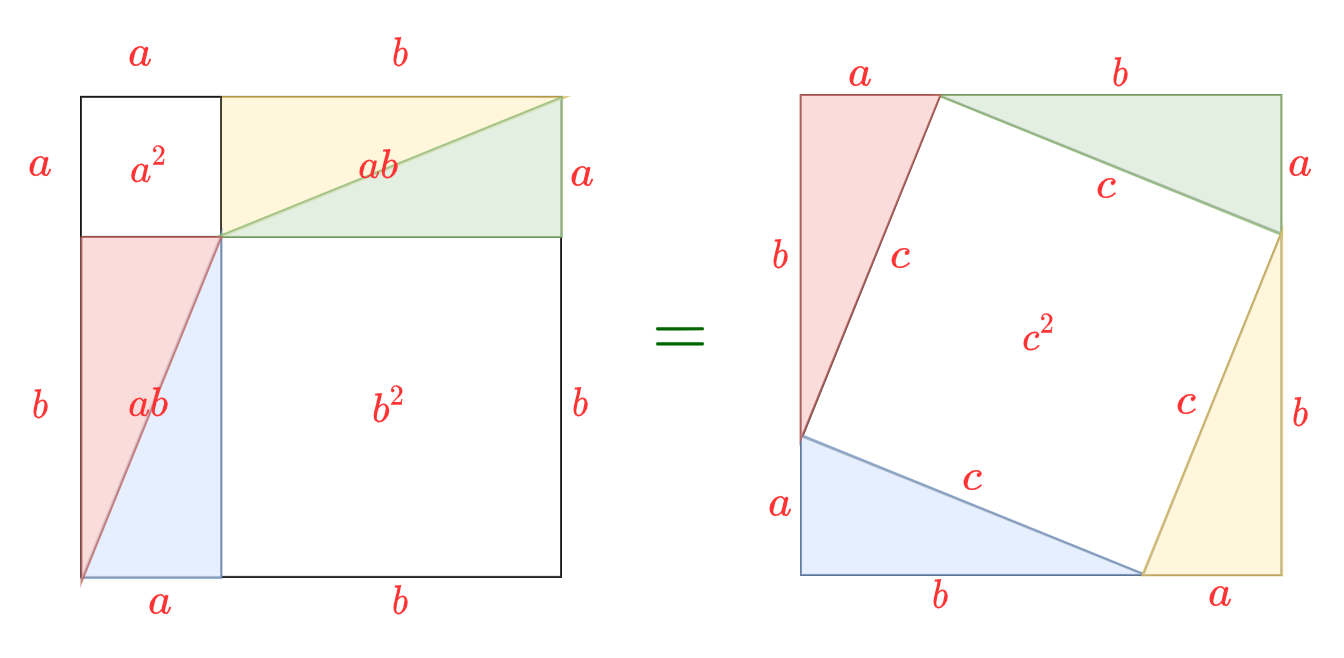
\includegraphics[scale=0.25]{pithagor.png}
\end{center}
\caption{}\label{pithagor}
\end{figure}

\item \textbf{Разность квадратов}. Визуализация $(a-b)(a+b)=a^2-b^2$ (рис. \ref{razn}).
\begin{figure}[hbt!]
\begin{center}
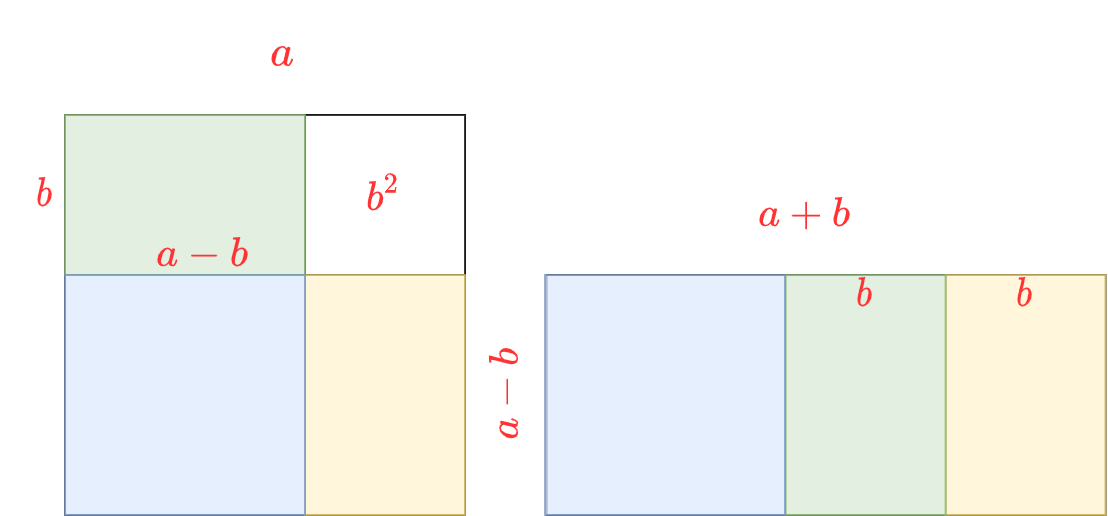
\includegraphics[scale=0.25]{razn.png}
\end{center}
\caption{}\label{razn}
\end{figure}

\item \textbf{Сумма подряд идущих чисел} $1,2,\dots,n$. Решаем для случая четного $n$.
Расставляем прямоугольники $1\times k$ лесенкой от самого маленького к самому большому (рис. \ref{ariphm}). Далее замечаем, что если последний переложить на первый, предпоследний на второй, и т.д., то будут получаться одинаковые прямоугольники высотой $n+1$. Получится $n/2$ прямоугольников длины $n+1$, так что сумма равна $n(n+1)/2$.

\begin{figure}[hbt!]
\begin{center}
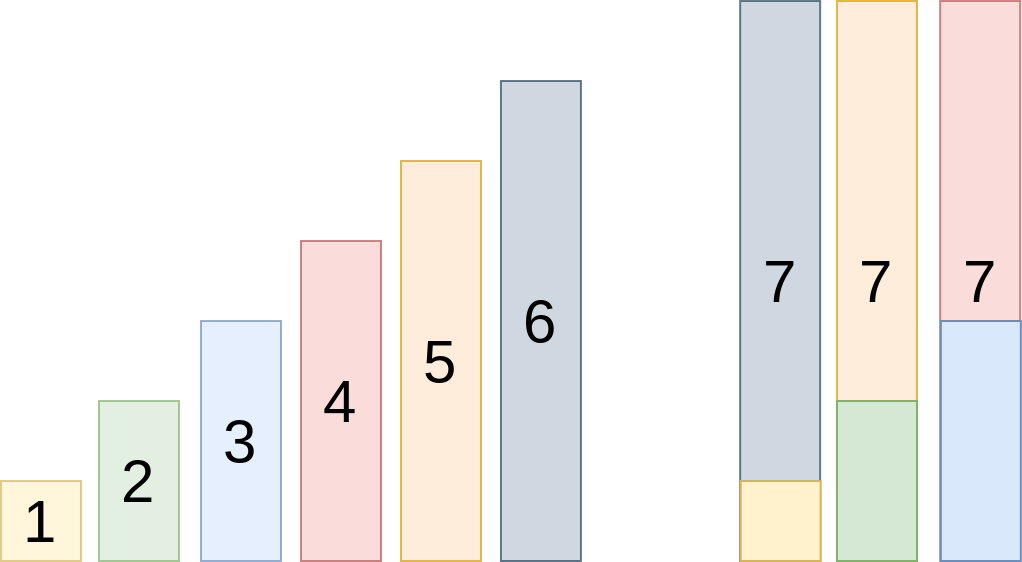
\includegraphics[scale=0.2]{ariphm.png}
\end{center}
\caption{}\label{ariphm}
\end{figure}

Если $n$ --- нечетное, то применим тот же метод, отставив в сторону последнее слагаемое $n$. Получится $(n-1)/2$ столбиков высотой $n$ и плюс еще один столбик высотой $n$. Итого, снова будем иметь сумму $n(n+1)/2$

\item \textbf{Бинома Ньютона для} $n=3$: $(a+b)^3 = a^3+3a^2b+3ab^2+b^3$. Разрезание сырного кубика на 8 частей тремя плоскостями. См. рис. \ref{kub}

\begin{figure}[hbt!]
\begin{center}
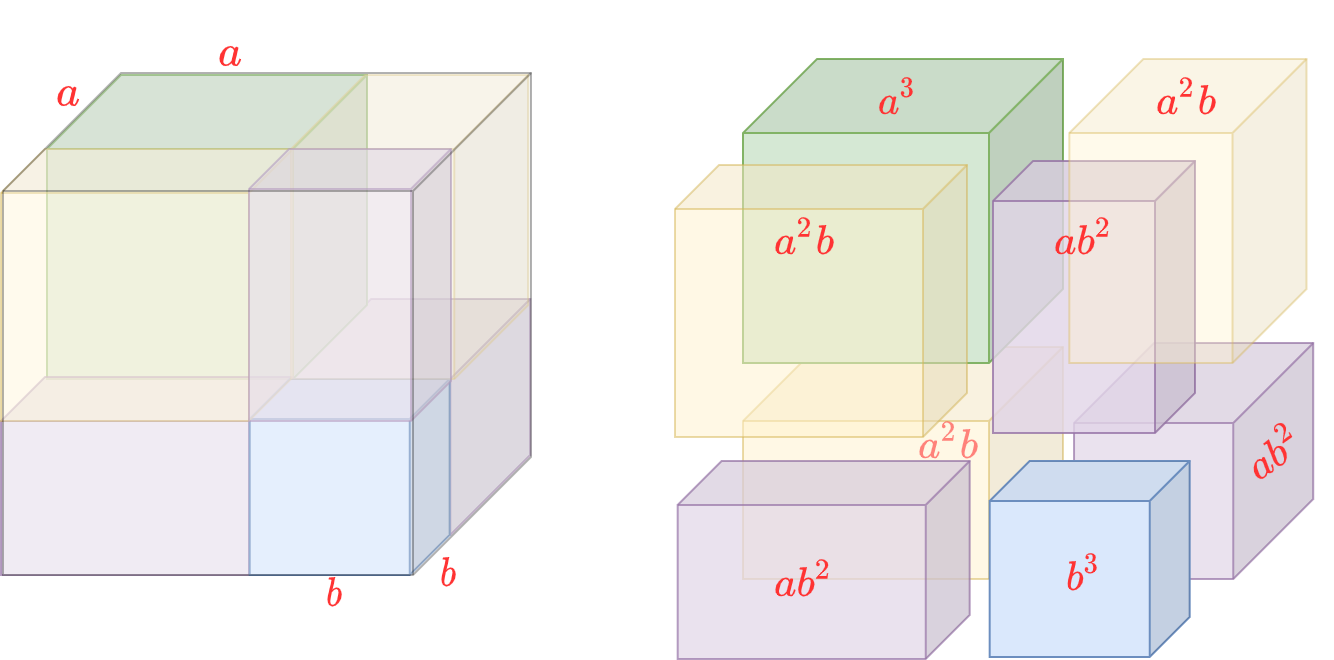
\includegraphics[scale=0.25]{kub.png}
\end{center}
\caption{}\label{kub}
\end{figure}
\end{enumerate}

\subsection*{Задачи}

\begin{enumerate}
\item Найти с помощью графического метода сумму подряд идущих нечетных чисел от 1 до $n$, где $n$ --- нечетное.
\end{enumerate}


\section{Соизмеримость отрезков, алгоритм Евклида}


\lesson{Соизмеримость отрезков. Кузнечики и визуальный алгоритм Евклида}

\begin{enumerate}
\item Пусть у нас на числовой прямой сидят в точке $O$ два кузнечика. Один умеет прыгать на длину $a$ как вправо, так и влево, а второй --- на длину $b$ как вправо, так и влево.

\item Могут ли они через какое-то конечное количество прыжков попасть в одну и ту же точку, отличную от $O$?
\item Ответ --- да, если есть такая точка $A$, что отрезок $OA$ кратен и $a$, и $b$ одновременно, т.е. при некотрых натуральных $n,m$, не равных нулю, будет верно равенство $an=bm$:
$$
\underbrace{a+a+\dots+a}_{n\mbox{ раз}}=\underbrace{b+b+\dots+b}_{m\mbox{ раз}}
$$
\item Отрезки, которые имеют общий кратный отрезок, называются \textbf{соизмеримыми}.\index{Соизмеримость}
\item Из равенства $an=bm$ видно, что есть общий отрезок $c=a/m=b/n$, который целое число раз укладывается как в $a$, так и в $b$. Такой отрезок $c$ называется \textbf{наибольшим общим делителем} $a$ и $b$ и обозначается $\gcd(a,b)$. Ясно, что он существует тогда и только тогда, когда существует отрезок $OA$, кратный отрезкам $a$ и $b$.

Действительно, если $c=\gcd(a,b)$ существует, то он, являясь делителем, имеет представление $c=a/m=b/n$ при некоторых положительных натуральных $n,m$, откуда $an=bm$, и отрезок $OA$ длины $an$ является искомым. Обратно, если существует отрезок $OA$, одновременно кратный как $a$, так и $b$, то имеет место представление $OA=an=bm$, откуда число $c=a/m=b/n$ является делителем как $a$, так и $b$, а значит, их общим делителем, следовательно, существует и $\gcd(a,b)$.

\item На этот отрезок можно выйти другим путем: строим прямоугольник $a\times b$ ($a<b$), начинаем отсекать в нем квадраты: сначала отсекаем квадраты $a\times a$, пока можем, останется кусок $a\times b_1$ ($b_1<a$), затем отсекаем квадраты $b_1\times b_1$, пока можем, останется кусок $a_1\times b_1$ ($a_1<b_1$), и т.д.
\begin{figure}[hbt!]
\begin{center}
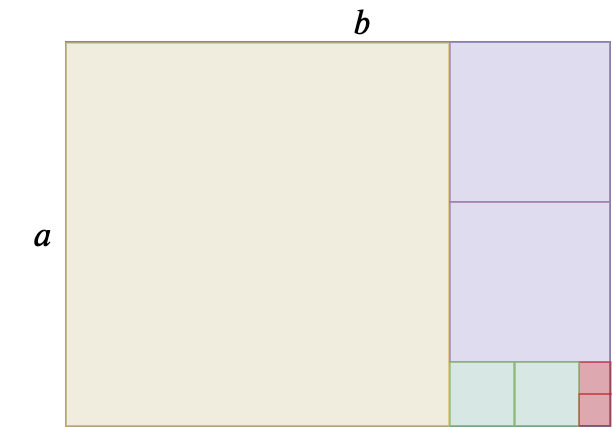
\includegraphics[scale=0.3]{soizmer.png}
\end{center}
\caption{}\label{soizmer}
\end{figure}

\item Если исходные отрезки соизмеримы, то процесс остановится: исходный прямоугольник будет разбит на конечное число квадратиков. При этом можно заметить, что самые мелкие квадратики целое число раз укладываются во все более крупные просто по построению. Это значит, что прямоугольник $a\times b$ можно разбить на конечное число маленьких квадратиков, общее число которых будет $nm$ штук.

Действительно, соизмеримость $a$ и $b$ означает, что стороны прямоугольника можно разбить на целое число частей длины $c=a/m=b/n$, а процесс разрезания этого прямоугольника на квадраты всегда будет происходить по сетке с шагом $c$, причем каждый раз шаг разрезания будет уменьшаться. Но у нас конечное число квадратиков $c\times c$, стало быть, процесс разрезания рано или поздно упрется в прямоугольник со стороной $c$, который уже будет разделен на целое число квадратов. На этом алгоритм и закончится.

\item Длина стороны финального квадратика будет иллюстрировать НОД отрезков $a$ и $b$, т.к. это максимальный квадрат, которым можно замостить прямоугольник $a\times b$. 

Действительно, любой квадрат, которым можно замостить прямоугольник $a\times b$, целое число раз укладывается в квадрат $a\times a$ и, как следствие, в оставшийся прямоугольник $a\times(b-a)$, а значит, целое число раз укладывается в квадрат $(b-a)\times (b-a)$ и, как следствие, в оставшийся прямоугольник, и т.д. То есть, если каким-то квадратом можно замостить исходный прямоугольник, то им же можно замостить и финальный маленький квадратик. Следовательно, этот квадратик наибольший из всех таких. которыми можно замостить прямоугольник $a\times b$.
\item Такой процесс постепенного спуска к НОД называется \textbf{алгоритмом Евклида},\index{Алгоритм Евклида} к нему мы еще неоднократно вернемся с более формальной точки зрения.
\item Заметим, что числа $a$ и $b$ при этом вовсе не обязаны быть натуральными. Это --- какие-то векторы на числовой прямой. в том числе они могут быть отрицательными (при этом их НОД, если он существует, всегда выбирается со знаком плюс).
\end{enumerate}
\subsection*{Задачи}
\begin{enumerate}
\item Найти НОД(10,6) методом прямоугольников.
\item Сколько и каких шагов должны сделать 10- и 6-шаговые кузнечики, чтобы попасть в точку НОД(10,6)?
\end{enumerate}


\begin{comment}
\chapter{2. Движения прямой}
\end{comment}
\newchapter{Движения прямой}

\vrezka{В этой главе мы переходим к более формальной работе с точками и векторами на прямой. Целью является знакомство с понятиями <<движение>>, <<композиция движений>>. Проводится полный анализ видов движений и свойств их композиций.

Попутно вводится понятие группы и подгруппы в приложении к группе движений на прямой. Изучаются все конечные подгруппы движений прямой.\index{Движения!прямой}
}

\section{Сдвиг, композиция сдвигов, группа}

\lesson{Иллюстрация сдвигов с помощью линейной парковки. Обозначения сдвигов. Композиция сдвигов. $\id$ и обратный сдвиг. Фрмулировка аксиом группы}


\begin{enumerate}
\item \textbf{Иллюстративная сказка}. Представим себе очень длинную однорядную автомобильную парковку на территории какого-нибудь бизнес-центра. На этой парковке размечены места номерами 0, 1, 2 и т.д. (слева направо). В какой-то момент парковку достроили влево и решили, не мудрствуя лукаво, продолжить нумерацию отрицательными числами $-1$, $-2$, $-3$ и т.д. Получилась шкала примерно как на градуснике для измерения уличной температуры. Водителям, работающим в этом бизнес-центре, выдали парковочные талоны с номерами парковочных мест, т.е. такие же числа 0, $\pm 1$, $\pm 2$ и т.д. В соответствии с талонами они занимают свои места, так что получается, что водитель с талоном номер 0 встает на место номер 0, водитель с талоном номер 1 --- на место номер 1 и т.д.
\item Но потом появляется необходимость поменять бордюр и плитку там, где находятся два крайних левых парковочных места, пусть это будут номера $-3$ и $-2$. Возникает потребность куда-то девать те а/м, для которых зарезервированы номера $-3$ и $-2$. Вместо того, чтобы предложить обменять талоны $-3$ и $-2$ на резервные номера парковки, начальнику охраны приходит в голову гениальная идея: повесить на въезде плакат с надписью (красным фломастером на А4): <<Внимание! Занимайте номер парковки на 2 больше, чем указан в вашем талоне!!>>
\item Так что водитель, имеющий парковочный талон номер -3, занимает место -1, номер -2 --- место 0, номер -1 --- место 1, и т.д.

\begin{figure}[hbt!]
\begin{center}
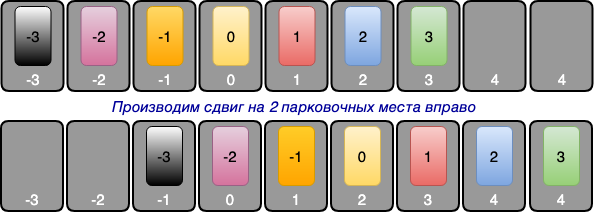
\includegraphics[scale=0.3]{TT.png}
\end{center}
\caption{}\label{TT}
\end{figure}
\item Иначе говоря, все автомобили должны теперь вставать на 2 места правее, т.е. произвести сдвиг относительно своего обычного места, указанного в парковочных талонах (см. рис. \ref{TT}).
\item Отметим еще одну особенность истории с парковкой: несмотря на произведенное перемещение автомобилей, они по-прежнему остаются на парковке, не занимая места где-либо еще, например, на проезжей части или тротуаре. Просто потому, что запас мест справа оказался достаточным для данной манипуляции.
\item А что, если бы парковка была неограниченно расширяемой в обе стороны автоматически всякий раз, когда не хватает места? Как говорят математики, она была бы потенциально бесконечной.
\item Геометрически мы можем представить это так: у нас имеется прямая, на которой нанесена разметка числами 0, $\pm 1$, $\pm 2$ и т.д. через равные расстояния между соседними точками. Прямая --- бесконечная в обе стороны. Но вдруг возникает необходимость сдвинуть эту прямую вправо на 2 единицы. Для этого всем точкам прямой дается команда сдвинуться на вектор длины 2 вправо.
\item Однако, чтобы сохранить историю этого сдвига и проверить его правильность, следует сдвигать не саму прямую, а ее копию. В итоге мы получаем прямую-оригинал и прямую-образ. Если уж быть совсем точными, то у нас возникает то, что в математике называется функцией, т.е. соответствие между оригинальными точками и их точками-образами на копии прямой.
\item Так мы видим не только новое положение точек, после сдвига, но и как оно соотносится с прежним их положением!
\item Понятно, что сдвигать геометрическую прямую, не выходя за ее пределы, можно только вправо или влево, причем на вектор произвольной длины, не обязательно на число 2 или 3, или им подобное. Тем более что цифровую разметку на прямую можно и вовсе не наносить.
\item Преобразование, состоящее в том, что все точки прямой сдвигаются на вектор $a$, называется \textbf{сдвигом} на вектор $a$. При этом, чтобы узнать, в какую точку (относительно исходной разметки) перейдет точка $A$, нужно от точки $A$ отложить вектор $a$, т.е. найти сумму $A+a$. Это будет некоторая точка $A'$ на этой же прямой.
\item Преобразование сдвига на вектор $a$ обозначим $T_a$, а его действие на точку $A$ обозначим $T_a(A)$. Так что
$$
T_a(A)=A',\quad a=\vec{AA'}.
$$
\item Сдвиг является движением (не случайно это однокоренные слова!).
\item Вообще, \textbf{движение --- это преобразование, сохраняющее расстояния}\index{Движение} (размеры и форму): если между точками $A$ и $B$ было расстояние $x$, то после преобразования движения расстояние между точками $A'$ и $B'$, в которые перешли исходные точки, тоже будет $x$, и так для любой пары точек! Для сдвига эот очевидно, поскольку ко всем точкам прибавляется один и тот же вектор.
\item Математическое движение --- это результат физического движения (есть только начальное и конечное состояние системы).
\item Сдвиг характерен тем, что он в качестве параметра имеет только вектор, т.е. величину и направление сдвига, но он никак не связан с исходной разметкой прямой!
\item Композиция сдвигов --- это их последовательное применение:
\begin{equation}\label{Tcomposition}
(T_b\circ T_a)(A)=T_b(T_a(A)).
\end{equation}
\item Композиция сдвигов соответствует сумме векторов: $T_b\circ T_a=T_{a+b}$.
\item Композиция сдвигов перестановочна в силу коммутативности сложения: $$T_b\circ T_a=T_a\circ T_b.$$
\item Композиция сдвигов ассоциативна, т.е. если мы имеем последовательность из трех и более сдвигов, то мы можем начать вычислять ее с любого места цепочки, постепенно сворачивая выражение, как с обычными числами:
$$
T_a\circ T_b\circ T_c = (T_a\circ T_b)\circ T_c = T_a\circ (T_b\circ T_c),
$$
т.е. сначала вычислить композицию последних и результат подставить в первую, либо же наоборот --- сначала вычислить первую, и ее применить к последней. Это правило можно тиражировать на цепочку композиций любой длины. Результат при этом будет один и тот же, совершенно так же, как если бы мы складывали подряд несколько чисел.
\item Кратность сдвига обозначается как степень
$$
\underbrace{T_a\circ\dots\circ T_a}_{n\mbox{ раз}}=T_a^n
$$
и соответствует кратности сложения или сдвигу на вектор, получаемый умножением исходного вектора на степень кратности: $T_a^n=T_{an}$.
\item Нулевой сдвиг $T_0=\id$ --- это \textbf{тождественное преобразование}, которое ничего не меняет.
\item Обратный сдвиг $T_a^{-1}$ --- это сдвиг на вектор $-a$, т.е. сдвиг в обратном направлении на ту же величину.
\item Нулевой сдвиг сам себе обратен.
\item Вообще, если есть какие-то два преобразования $u$ и $v$ и операция композиции $\circ$, то эти преобразования \textbf{взаимно обратны}, если $u\circ v=\id$ и $v\circ u=\id$, т.е. последовательное применение этих преобразований в любом порядке является тождественным преобразованием (сводится к ничего не деланию).
\item Обобщая свойства сдвигов, фиксируем понятие \textbf{группы}.\index{Группа} Это --- такое множество $G$ с заданной на нем одной бинарной операцией $\circ$, для которой выполняются аксиомы:
\begin{enumerate}[{\bf G}1)]
\item Результат групповой операции снова лежит в этом же множестве (например, композиция сдвигов есть сдвиг):
$$
u,v\in G \Rightarrow u\circ v\in G.
$$
\item Групповая операция \textbf{ассоциативна} (сочетательный закон): для любых элементов $u,v,w$ группы $G$\index{Ассоциативность}
$$
(u\circ v)\circ w = u\circ (v\circ w)
$$
(например, $(T_a\circ T_b)\circ T_c=T_a\circ(T_b\circ T_c)$.
\item Существует \textbf{нейтральный элемент} $\id$ такой, что для любого элемента $u$ имеет место равенство\index{Нейтральный элемент}
$$
u\circ\id = u = \id\circ u.
$$
\item Групповая операция \textbf{обратима}: для всякого элемента $u$ существует обратный ему элемент $v$ такой, что
$$
u\circ v=\id = v\circ u
$$
(например, обратный сдвиг --- это сдвиг в противоположную сторону:  $T_{a}^{-1}=T_{-a}$). Элемент $v$ в таком случае обозначается как $u^{-1}$ и называется \textbf{обратным} к элементу $u$.\index{Обратный элемент}
\end{enumerate}
\item Множество всех сдвигов образует группу относительно операции композиции!
\item Мало того, группа сдвигов \textbf{коммутативна}\index{Коммутативность} (абелева), т.е. для ее групповой операции выполняется переместительный закон:\index{Группа!абелева}
\begin{enumerate}[resume*]
\item $u\circ v=v\circ u$ для всех $u,v$ из группы $G$.
\end{enumerate}
\item Кратность обратного сдвига: $T_a^{-n}= (T_a^{-1})^n=T_{-a}^n=T_{-an}=(T_{an})^{-1}$.
\item Обратный сдвиг к композиции сдвигов: $(T_a\circ T_b)^{-1}=T_b\circ T_a$. Это легко следует из общего свойства группы:
$$
(u\circ v)^{-1} = v^{-1}\circ u^{-1},\mbox{ поскольку }(u\circ v)\circ(v^{-1}\circ u^{-1})=u\circ(v\circ v^{-1})\circ u=\id.
$$
\item На основе только одного сдвига $T_a$ можно построить подгруппу сдвигов
$$
\langle T_a\rangle = \{T_a^n, T_a^{-n}\mid n=0,1,2,\dots\}
$$
\item Эта подгруппа --- реализация целых чисел $\Z$, к которым мы еще вернемся позже.
\item Фиксируем понятие \textbf{подгруппы}.\index{Подгруппа} Это --- подмножество группы, на котором групповая операция удовлетворяет групповым аксиомам, т.е. подгруппа сама является группой с той же операцией, которая задана в группе.\label{Subgroup}

Подгруппу можно определить иначе: непустое подмножество $H\subseteq G$ группы $G$ называется подгруппой, если для любых $a,b\in H$ имеет место $a\circ b^{-1}\in H$.

Оба определения эквивалентны. Действительно, если $H$ удовлетворяет первому определению, т.е. само является группой, то требование $(a,b\in H)\to (a\circ b^{-1}\in H)$ выполняется по определению группы автоматически. Обратно, если данное требование выполнено, то, очевидно, что единица группы $G$ принадлежит $H$ ($a\circ a^{-1}\in H$), обратный элемент к элементу $b\in H$ также принадлежит $H$, т.к. $\id\circ b^{-1}\in H$, ассоциативность операции наследуется от группы $G$,
замкнутость операции $(a,b\in H)\to (a\circ b\in H)$ проверяется непосредственно, если воспользоваться тем, что $a\circ b=a\circ (b^{-1})^{-1}$.


\item Каждый сдвиг $T_a$ порождает (с помощью его многократного тиражирования) свою подгруппу в группе всех сдвигов.
\end{enumerate}


\section{Отражение}

\lesson{Иллюстрация отражения через парковку а/м. Композиция сдвигов и отражений}


\begin{enumerate}
\item Продолжим нашу историю с движением автомобилей. Пусть на сей раз вместо парковки они готовятся к параду и должны занять свои места в ряду с номерами 0, $\pm 1$, $\pm 2$ и т.д. Номера мест нанесены, как и ранее, на асфальт и представляют собой один ряд. У водителей а/м есть предписания, в которых указано, какие места нужно занять. Следующим шагом предписания является команда обменяться местами так, чтобы порядок а/м сменился на противоположный. Иначе говоря, каждому нужно проехать полукруг и занять место, симметричное относительно заданного. Например, центром симметрии и соответствующих полукругов является место 0. Тогда а/м, стоящий на 1-м месте, должен переехать на место $-1$, стоящий на 2-м месте --- на место $-2$, и т.д.
\item В результате мы получим перестроение на параде, при котором а/м опишут полукруги и встанут в обратном порядке, причем нулевой а/м сохранит свое место (см. рис. \ref{SST}).
\begin{figure}[hbt!]
\begin{center}
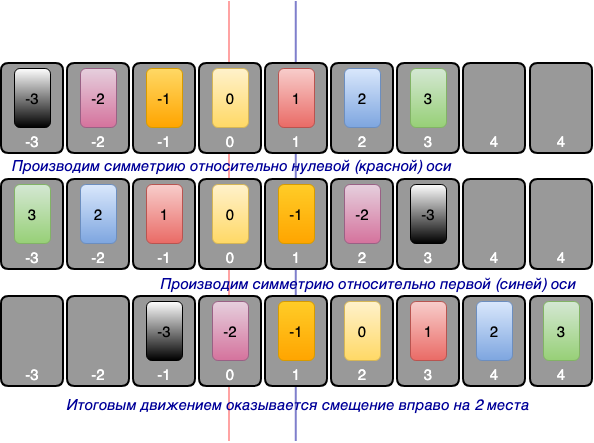
\includegraphics[scale=0.3]{SST.png}
\end{center}
\caption{}\label{SST}
\end{figure}
\item Заметим, что и в этом случае расстояние между а/м сохранится: как было ранее 2 а/м между 0-м и 3-м, так и останется. И так для всех пар автомобилей.
\item Такой вид движений называется \textbf{отражением}. Вся наша линейная парковка отразилась относительно нулевого места.
\item Особо отметим, что физически отражение всегда требует выхода за пределы исходной фигуры. Если сдвиг мы могли осуществить, находясь внутри парковочной сетки (ну, да, предположим, что мы имеем дело с танками, которые могут на месте повернуться на 90 градусов, произвести перемещение, а затем развернуться снова, либо что имеем дело с параллельной парковкой, где а/м стоят вдоль направления нумерации), то отражение никак невозможно выполнить, оставаясь в пределах исходной парковки --- потребуется выезд на проезжую часть.
\item Отражение на геометрической прямой --- то же самое. Сначала мы должны выбрать центр отражения, который останется на месте, затем перевернуть прямую в обратном направлении (снова имеем выход во внешнее пространство, если представить отражение как физический процесс!).
\item Отражение с центром в точке $O$ будем обозначать $S_O$. Отражение можно представить как огромное количество сдвигов, выполняемых одновременно. Для каждой точки --- свой сдвиг, причем на разные векторы для разных точек. Так, в результате действия отражения $S_O$ на точку $A$ мы получим точку $A'=T_a(A)$, где вектор $a=2\vec{AO}$. То есть, мы производим сдвиг на расстояние $2|OA|$, только в противоположную от $A$ сторону.
\item Как и в случае со сдвигом, отражение --- это функция, т.е. оно <<помнит>> исходную разметку прямой, а значит, мы всегда можем сказать, какая точка откуда пришла в свое новое состояние.
\item Отражение, в отличие от сдвига, намертво привязано к одной выделенной точке на прямой \textit{в исходной разметке}, и полностью ею определяется! Мы можем рассмотреть два и более отражений, но все они должны быть заданы в одной исходной разметке прямой, чтобы не возникла путаница.
\item Композиция отражений и композиция отражения и сдвига определяются аналогично композиции сдвигов (см. \eqref{Tcomposition}):
$$
(S_O\circ S_A)(x) = S_O(S_A(x)),\quad (S_O\circ T_a)(x) = S_O(T_a(x)),\quad (T_a\circ S_O)(x) = T_a(S_O(x)),
$$
т.е. применение операций выполняется справа налево.
\item Отражение обратно самому себе: $S_O\circ S_O=\id$, т.е. $S_O^{-1}=S_O$.
\item В терминах парада, показанного на рисунке, все отражения задаются относительно разметки мест на асфальте! В этом случае водителям для выполнения операции отражения не нужно знать, где какие номера а/м находятся, им достаточно видеть номер своего парковочного места, знать номер места---центра симметрии, и выполнить перемещение на удвоенное расстояние, чтобы занять противоположное место (см. рис. \ref{SST}).
\item Поэтому композиция отражений, т.е. их последовательное применение, легко вычисляется:
\begin{equation}\label{SOSC}
S_O\circ S_C=T_{2CO},\quad S_C\circ S_O=T_{2OC}.
\end{equation}
Если вспомнить общее групповое правило $(u\circ v)^{-1} = v^{-1}\circ u^{-1}$, то второе равенство легко получить из первого:
$$
T_{2OC} = T_{2CO}^{-1} = (S_O\circ S_C)^{-1} = S_C^{-1}\circ S_O^{-1}=S_C\circ S_O.
$$
\item Заметим, что композиция отражений является сдвигом и при этом не коммутативна! То есть, отражения, производимые в разной последовательности, приводят, вообще говоря, к разным результирующим сдвигам, а именно --- к противоположным.



\section{Таблица композиций движений прямой}


\lesson{Составляем композиции отражений и сдвигов. Таблица композиций классов, аналог таблицы умножения знаков}


\item Композиция отражения и сдвига:
\begin{equation}\label{SOTa}
S_O\circ T_a = S_{O-a/2},\quad T_a\circ S_O = S_{O+a/2}.
\end{equation}

Это легко проверить, если вместо $a$ подставить $2CO$, и в предыдущих равенствах произвести необходимые домножения. Предлагаем это проделать самостоятельно.
\item Итак, композиция сдвига и отражения является отражением и при этом не коммутативна!
\item Таблица композиций отражений и сдвигов:\index{Группа!движений прямой}
\begin{center}
\begin{tabular}{c|c|c|}
  & $T_a$ & $S_O$ \\
 \hline
$T_b$ & $T_{a+b}$ & $S_{O+b/2}$ \\
 \hline
$S_C$ & $S_{C-a/2}$ & $T_{2OC}$ \\
\hline
\end{tabular}
\end{center}
Таблицу композиций следует читать слева наверх, т.е. если в левом столбце стоит движение $F$, а в верхней строке --- движение $G$, то в соответствующей ячейке стоит композиция $F\circ G$.
\item Кратность отражения $S_O^n$ определяется четностью числа $n$. В случае четного $n$ это $\id$, в случае нечетного --- исходное $S_O$.
\item Пара $\{\id, S_O\}$ образует самую маленькую нетривиальную группу движений, которая, к тому же, является абелевой и циклической (т.е. все ее элементы есть степени какого-то одного, а именно $S_O=S_O^1$, $\id=S_O^2=S_O^0$).
\begin{table}[htb!]\begin{center}
\begin{tabular}{c|c|c|}
  & $\id$ & $S_O$ \\
 \hline
$\id$ & $\id$ & $S_O$ \\
 \hline
$S_O$ & $S_O$ & $\id$ \\
\hline
\end{tabular}
\end{center}\end{table}
\item Видим, что таблица полностью повторяет таблицу умножения знаков, причем $\id$ является нейтральным элементом.
\item Суммируя, находим, что вообще все сдвиги и отражения вместе образуют группу (относительно операции композиции), т.е. для них выполняются аксиомы группы G1--G4. При этом данная группа не является абелевой (не выполняется G5), поскольку, как мы видели, далеко не все композиции движений перестановочны.
\item Еще пример группы: рассмотрим класс всех сдвигов $\T$ и класс всех отражений $\S$
\item Мы можем определить композицию классов $\T\circ \T$, $\T\circ \S$, $\S\circ \T$ и $\S\circ \S$ как все возможные композиции движений из этих классов в указанном порядке. Иначе говоря, композиции классов --- это их умножение по Минковскому:
$$
\T\circ \T = \{t\circ t'\mid (t\in\T)\land(t'\in\T)\},\quad \T\circ \S = \{t\circ s\mid (t\in\T)\land(s\in\S)\}
$$
$$
\S\circ \T = \{s\circ t\mid (s\in\S)\land(t\in\T)\},\quad \S\circ \S = \{s\circ s'\mid (s\in\S)\land(s'\in\S)\}
$$
\item Из произведенных выше вычислений легко видеть таблицу композиций этих классов:\index{Таблица композиций}
\begin{center}
\begin{tabular}{c|c|c|}
  & $\T$ & $\S$ \\
 \hline
$\T$ & $\T$ & $\S$ \\
 \hline
$\S$ & $\S$ & $\T$ \\
\hline
\end{tabular}
\end{center}
\item Видим полную аналогию с таблицей знаков и таблицей для $\id, S_O$. Здесь класс $\T$ является нейтральным элементом
\item Если теперь собрать в одну кучу все сдвиги и отражения, то получим группу движений прямой
\item Наша цель --- доказать, что других движений нет, т.е. что мнжество $\{T_a,S_O\}_{a,O}$ полностью исчерпывает все возможные движения прямой
\end{enumerate}

\subsection*{Задачи}

Пусть на прямой даны 4 точки $A,B,C,D$, поставленные друг за другом с одинаковым шагом (см. рис. \ref{ABCD}).
\begin{figure}[hbt!]
\begin{center}
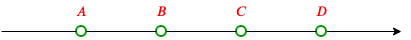
\includegraphics[scale=0.7]{ABCD.png}
\end{center}
\caption{}\label{ABCD}
\end{figure}

\begin{enumerate}
\item Куда перейдет точка $A$ при преобразовании $S_B$?
\item Куда перейдут точки $B,C,D$ при преобразовании $T_{AB}\circ T_{CA}$?
\item Куда перейдут точки $A,B,C$ при преобразовании $S_C\circ T_{AB}$?
\item Вывести равенства \eqref{SOTa} из равенств \eqref{SOSC}.
\end{enumerate}



\section{Теорема о гвоздях, аналог теоремы Шаля}


\lesson{Стационарные точки. Теорема Шаля}


\begin{enumerate}
\item Анализ движений проводится на основе наблюдений за количеством стационарных точек
\item Пусть движение $M$ таково, что оно оставляет на месте две точки $A\ne B$.
\item $M(A)=A$ и $M(B)=B$. Пусть $C'=M(C)$. $M$ сохраняет расстояния $AC$ и $BC$, откуда $AC=AC'$ и $BC=BC'$, откуда $C=C'$. Т.е. $M(C)=C$ для любых точек $C$, т.е. $M=\id$

\begin{figure}[hbt!]
\begin{center}
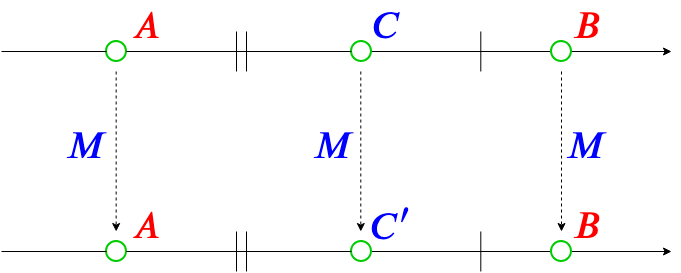
\includegraphics[scale=0.35]{LineMoving.png}
\end{center}
\caption{}\label{LineMoving}
\end{figure}
\item Пусть движение $M$ оставляет на месте ровно одну точку $O$. В этом случае $A'=M(A)$ и $A\ne A'$ и $OA=OA'$, тогда $A'$ --- отражение $A$ относительно $O$. Следовательно, $M=S_O$
\begin{figure}[hbt!]
\begin{center}
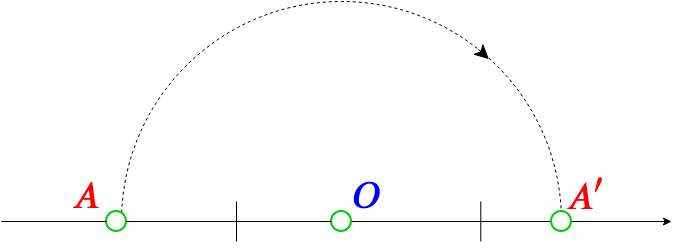
\includegraphics[scale=0.35]{LineMovingO.png}
\end{center}
\caption{}\label{LineMovingO}
\end{figure}

\item Пусть движение $M$ не оставляет на месте ни одной точки и пусть $B=M(A)$ ($B\ne A$). Обозначим $x=AB$. Тогда $T_{x}^{-1}\circ M(A)=A$, т.е. $T_{x}^{-1}\circ M$ оставляет на месте хотя бы одну точку $A$.
\begin{figure}[hbt!]
\begin{center}
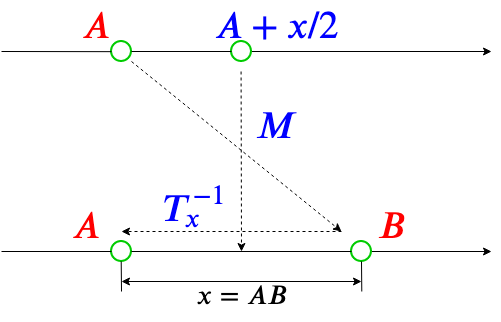
\includegraphics[scale=0.35]{LineMovingx.png}
\end{center}
\caption{}\label{LineMovingx}
\end{figure}

Если оно оставляет на месте ровно одну точку $A$, то это некоторое отражение $S_A$, но тогда $M=T_x\circ S_A=S_{A+x/2}$. Получается, что $M$ сохраняет точку $A+x/2$ на месте. Противоречие. Остается вариант, что $T_{x}^{-1}\circ M$ оставляет на месте как минимум две точки, но тогда $T_{x}^{-1}\circ M=\id$, откуда $M=T_x\circ \id=T_x$ --- сдвиг.
\item Таким образом, все движения прямой --- это либо сдвиги (в частности, $\id$), либо отражения (теорема Шаля).\index{Теорема!Шаля}
\item При этом любое движение --- это либо одно отражение, либо композиция двух отражений.
\end{enumerate}
\subsection*{Задачи}
\begin{enumerate}
\item Построить сдвиг на 7 единиц вправо с помощью композиции двух симметрий.
\item Каким движением является следующая композиция?
$$
S_{O+n}\circ S_{O+n-1}\circ \dots\circ S_{O+1}\circ S_O.
$$
Ответ получить в зависимости от четности $n$.
\end{enumerate}


\section{Все конечные подгруппы движений прямой}



\lesson{Описание всех вариантов, как может сложиться конечная подгруппа движений}

\begin{enumerate}
\item Имея дело с группой движений, мы можем выделить несколько ее собственных подгрупп (определение и разбор понятия подгруппы см. на стр. \pageref{Subgroup}):
\begin{itemize}
\item подгруппа всех сдвигов --- бесконечная коммутативная группа;
\item подгруппа, порожденная одним сдвигом $\langle T_a\rangle$ --- тоже бесконечная коммутативная группа;
\item подгруппа одного отражения $\{\id, S_O\}$ --- конечная группа, состоящая из двух элементов, также коммутативная;
\item тривиальная подгруппа $\{\id\}$.
\end{itemize}
\item Возникает вопрос: а существуют ли промежуточные по размеру конечные подгруппы группы движений? Попробуем описать все конечные подгруппы движений прямой.
\item Пусть $H$ --- конечная подгруппа группы движений прямой.

Ранее (см. стр.  \pageref{Subgroup}) мы рассматривали два определения подгруппы: 1) как подмножества, являющегося группой относительно той же операции, 2) как непустого подмножества $H$, в котором $ab^{-1}\in H$ при $a,b\in H$. В случае конечной подгруппы определение можно упростить еще больше, а именно, заменить $ab^{-1}$ на банальное $ab$.

Итак, непустое конечное(!) подмножество $H$ группы $G$ образует подгруппу группы $G$, если для любых $a,b\in H$ имеет место $ab\in H$, т.е. если $H$ замкнуто относительно групповой операции.

Почему это так? Здесь нам на помощь приходит принцип Дирихле. Пусть в множестве $H$ ровно $n$ элементов ($n>0$). Возьмем какой-то элемент $h\in H$ и рассмотрим все его натуральные степени относительно групповой операции: $h, h\circ h, h\circ h\circ h$ и т.д. Ясно, что мы можем построить сколь угодно длинные композиции, в том числе, содержащие $n$ и более вхождений элемента $h$. Возьмем тогда первые $n+1$ таких композиций. Все они, по условию, являются элементами множества $H$, т.е. совпадают с одним из его $n$ элементов. Но тогда в силу принципа Дирихле найдется как минимум две равных композиции. Пусть в одной из них $k$ вхождений $h$, а в другой $j$, причем $k<j$:
$$
\underbrace{h\circ h\circ\dots\circ h\circ h}_{k} = \underbrace{h\circ h\circ\dots\circ h\circ h}_{j}.
$$
Пользуясь тем, что в группе $G$ есть обратный элемент $h^{-1}$, домножим это равенство справа $k$ раз на $h^{-1}$, в итоге получим
$$
\id = \underbrace{h\circ h\circ\dots\circ h\circ h}_{j-k}.
$$
Справа --- композиция элементов из $H$, а значит, принадлежит $H$, откуда следует, что $\id$ исходной группы $G$ находится в $H$. Далее, мы можем еще раз умножить полученное равенство на $h^{-1}$, и получим
$$
h^{-1} = \underbrace{h\circ h\circ\dots\circ h\circ h}_{j-k-1},
$$
где $j-k-1\ge 0$. Справа --- либо композиция элементов из $H$, либо $\id$, который также принадлежит $H$ по доказанному. Но тогда и $h^{-1}\in H$. Так что, всякий элемент входит в $H$ вместе со своим обратным. А отсюда уже следует, что $H$ удовлетворяет второму определению подгруппы, и по доказанному на стр. \pageref{Subgroup} является группой с той же операцией и единицей, что и в группе $G$.

\item Итак, пусть $H$ --- непустое конечное подмножество группы движений прямой, замкнутое относительно операции композиции. Как мы только что выяснили, $H$ является подгруппой группы движений.

Таким образом, во-первых, $\id$ есть элемент $H$.

\item Во-вторых, никакой сдвиг $T_a$ при ненулевом $a$ не может быть элементом $H$, иначе в $H$ окажутся все степени $T_a$, т.е. $\langle T_a\rangle \subseteq H$, и $H$ будет бесконечной.
\item В-третьих, если в $H$ есть хотя бы два различных отражения $S_A$ и $S_B$ ($A\ne B$), то и их композиция также находится в $H$, но это ненулевой сдвиг $T_{2AB}$, а все такие сдвиги мы исключили чуть выше. Следовательно, если в группе $H$ и есть отражение, то только одно.
\item Таким образом, либо $H=\{\id\}$ (тривиальная группа), либо $H=\{\id, S_O\}$ при некотором отражении $S_O$.
\end{enumerate}

\begin{comment}
\chapter{3. Вокруг окружности}
\end{comment}

\newchapter{Вокруг окружности}

\vrezka{В этой главе мы расширяем сферу деятельности и переходим к движениям окружности. Снова изучаем виды движений, строим таблицу композиций, доказываем теорему Шаля.

Попутно сопоставляем движения окружности с движениями прямой, выходим на отрицательные степени композиций и их арифметические свойства, как следствие, получаем целые числа другим путем.

По аналогии с натуральными числами говорим о том, что целые числа --- это и степени композиций движений, и мера длины, только оснащенная знаком, т.е. направлением измерения длины.
}

\section{Движения окружности}


\lesson{Иллюстрация движений окружности: повороты и отражения. Некоторые повороты, примененные несколько раз, дают нулевой поворот. Композиция поворотов}

\begin{enumerate}
\item \textbf{Иллюстративная сказка}. Вспомним песенку <<встаньте, дети, встаньте в круг!>> Представим, что много-много детей в спортивном зале выстроились в круг и начали водить хоровод. При этом в центре круга стоит воспитательница, так что все дети держатся на равном от нее расстоянии и смотрят на нее. Какое они осуществляют движение в зале? Они ходит под одной и той же окружности то в одну сторону, то в другую. И если мы поместим себя на место воспитательницы, то поймем, что хоровод просто вращается вокруг одного центра то влево, то вправо.\index{Движения!окружности}

Добавим к этому мероприятию драйва. В зале на полу прочерчена линия, которая делит его пополам на два прямоугольника. По хлопку в ладоши дети перебегают на противоположную сторону зала, т.е. они все бегут по прямым параллельным линиям, перпендикулярно линии, нарисованной на полу (примерно так же люди переходят зебру при переходе улицы по зеленому сигналу светофора). При этом каждый из них считает число шагов до линии, а затем продолжает движение в том же направлении еще на столько же шагов. Дойдя до конца, все разворачиваются так, чтобы снова видеть воспитательницу.

В итоге они снова образуют круг, только вывернутый наизнанку, т.к. у каждого участника круга сосед, стоявший слева, теперь стоит справа, и наоборот! Такое действие с кругом называется отражением. При этом, тот факт, что соседи поменялись местами, говорит нам о некотором необычном движении, а именно, о движении, меняющем ориентацию (перепутали право и лево).

\item Формализуем это с геометрической точки зрения. Берем окружность. Какие у нее есть движения, переводящие ее в саму себя?
\item Прежде всего, повторим, что движение --- это преобразование, сохраняющее расстояния (изометрия). Поэтому, если мы говорим о движении, переводящем фигуру (прямую, круг, квадрат, многоугольник, плоскость и т.д.) в саму себя, то это значит, что мы берем копию этой фигуры и накладываем ее на оригинал до полного совмещения контуров. При этом допускается вертеть ее как угодно, лишь бы наложение фигур оказалось идеальным --- без выступов и впадин, без какой-либо деформации.
\item Для того, чтобы уточнить смысл определения движения, нужно зафиксировать способ измерения расстояний на окружности.  Расстоянием между точками окружности $A$ и $B$ мы будем называть длину меньшей из дуг, соединяющих эти точки (вместо длины дуги можно использовать величину соответствующего ей угла, измеренного в радианах или градусах).
\item Очевидно, что движениями окружности являются как минимум: вращение вокруг ее центра, а также отражение относительно прямых, проходящих через ее центр.
\item В некотором смысле окружность --- аналог прямой. Только эту прямую взяли за 2 конца и замкнули где-то на бесконечности.
\item Поэтому вращение окружности соответствует сдвигу прямой, а отражение окружности относительно прямой --- отражению на прямой относительно точки (можно считать ее отражением относительно перпендикулярной прямой).
\item Если представить, что на окружности большого радиуса живут маленькие одномерные математики, то для них окружность будет практически не отличима от прямой, и движения окружности они будут воспринимать именно как движения прямой.
\item Поворот на угол $\al$ мы обозначим за $R_\al$ (положительный --- против часовой стрелки), отражение относительно прямой, имеющей угол наклона $\ph$, обозначим за $S_\ph$ ($0\le\ph<180^o$). Угол наклона прямой измеряется от заданного раз и навсегда радиуса окружности, который можно считать точкой отсчета (аналог нуля на прямой). В качестве радиуса нулевого угла мы выберем горизонтальный радиус справа от центра окружности.
\item Ось отражения $S_\ph$ мы будем обозначать $l_\ph$ (см. рис. \ref{Rund3}).

\begin{figure}[hbt!]
\begin{center}
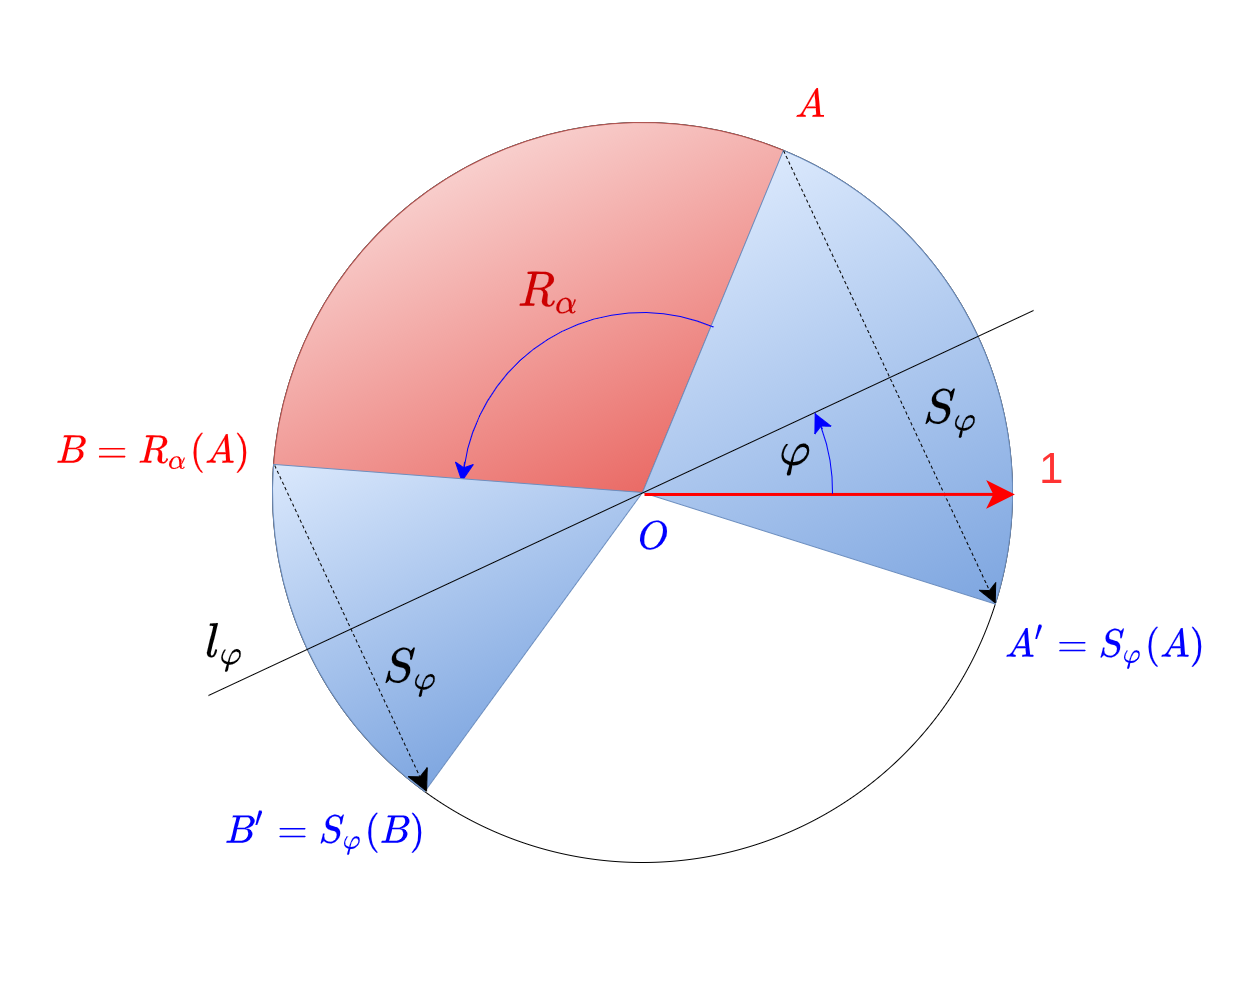
\includegraphics[scale=0.2]{Rund3.png}
\end{center}
\caption{}\label{Rund3}
\end{figure}

\item Вновь замечаем, что композиция поворотов есть поворот на суммарный угол: $R_\al\circ R_\be=R_{\al+\be}$
\item У каждого поворота есть обратный: $R_\al^{-1}=R_{-\al}$, т.н. поворот в противоположном направлении.
\item Повороты коммутируют: $R_\al\circ R_\be=R_\be\circ R_\al$.
\item Есть нейтральный поворот $\id=R_0$.
\item Так что все повороты образуют группу относительно операции композиции.
\item Тем не менее, есть одна особенность: поворот на угол $360^o$ (и все углы, кратные ему) --- это тоже $\id$.
\item Вообще, повороты, заданные углами с шагом $360^o$, равны друг другу:
$$
R_\al=R_{\al\pm 360^ok},
$$
где $k$ --- натуральное число.
\item Некоторые повороты дают $\id$ в некоторой степени, например, $R_{90^o}^4=\id$, $R_{60^o}^6=\id$ и т.д.
\item Если угол, выраженный в градусах, соизмерим с величиной $360^o$, то поворот на данный угол имеет положительную степень, в которой он обращается в $\id$.

Действительно, соизмеримость угла $\ph$ с углом $360^o$, как мы определяли ранее, означает, что существует некоторый угол $\psi$, кратный как $\ph$, так и $360$, т.е.
$$
\psi = \ph m = 360n.
$$
Но это и означает, что поворот $R_\ph$, возведенный в степень $m$, даст угол, кратный $360^o$, т.е. $\id$.

\item Но есть и такой угол $\ph$, который не соизмерим с углом $360^o$, и потому ни в какой степени не может дать $\id$. Это угол в 1 радиан.

Определение: угол $\ph$ равен 1 радиану, если длина дуги окружности, соответствующая данном углу, в точности равна радиусу этой окружности.

Когда угол измеряется в радианах, имеется ввиду, что мера угла есть длина соответствующей этому углу дуги единичной окружности. В частности, развернутому углу соответствует половина длины единичной окружности, обозначаемая числом $\pi$, так что угол $180^o$ --- это $\pi$ радиан.

Если бы угол в 1 радиан был соизмерим с полным оборотом, то число $\pi$ также оказалось бы соизмеримым с 1. Известно, однако, что это не так! Доказательство этого факта является сложной математической теоремой!

В свете сказанного, получем, что сколько бы раз мы ни откладывали угол в 1 радиан на окружности, мы никогда не окажемся в точке, соответствующей нулевому углу. Соответственно, группа вращений, порожденная степенями $R_{1\rad}$, является бесконечной. Позже мы докажем теорему о том, что углы поворота из этой группы образуют плотное множество, т.е. этими углами можно с любой точностью приблизить поворот на любой угол.

\item В зависимости от соизмеримости угла поворота с полным оборотом некоторые повороты порождают конечные циклические подгруппы в группе движений, а некоторые --- нет.
\end{enumerate}


\section{Группа движений окружности, теорема Шаля}\label{CircleGroup}

\lesson{Композиция отражений окружности. Таблица композиций движений окружности}

\begin{enumerate}\setlength{\itemsep}{1pt}
\item Композиция отражений: 
\begin{equation}\label{SSR}
S_\psi\circ S_\ph=R_{2(\psi-\ph)},\quad S_\ph\circ S_\psi=R_{2(\ph-\psi)}
\end{equation}
Например, второе равенство легко увидеть из картинки \ref{Rund}, где точка $A$ переходит в $A'$ под действием отражения $S_\psi$ относительно оси $l_\psi$, а затем $A'$ переходит в $A''$ под действием отражения $S_\ph$ относительно оси $l_\ph$:

\begin{figure}[hbt!]
\begin{center}
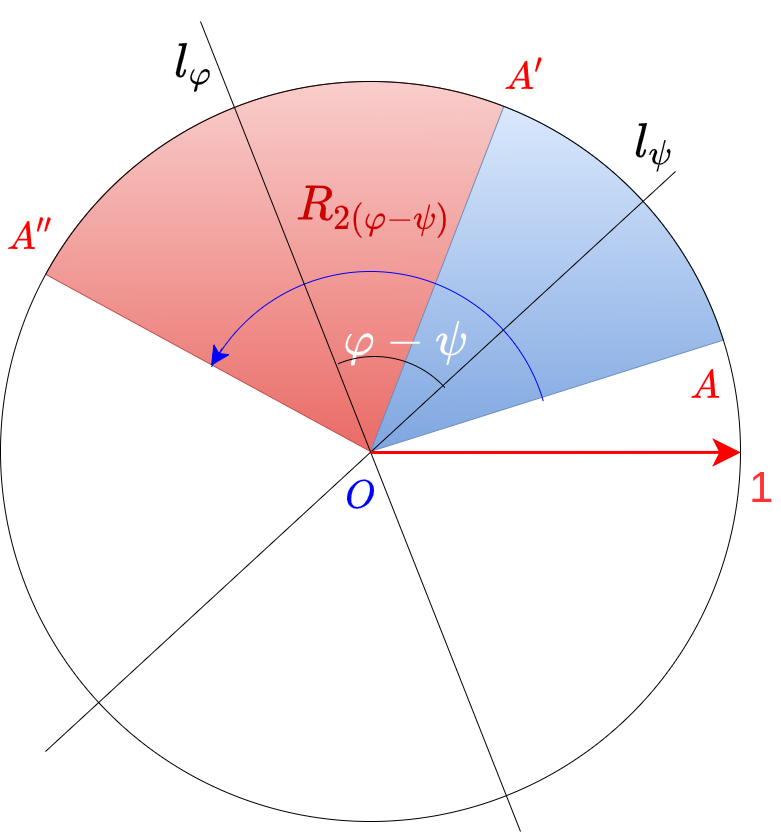
\includegraphics[scale=0.25]{Rund.png}
\end{center}
\caption{}\label{Rund}
\end{figure}

Суммарный угол поворота точки $A$ при переходе в точку $A''$ можно разбить на 2 пары углов так, что в каждой паре углы равны в силу свойств отражения (разные пары отмечены разным цветом), и в то же время угол между осями состоит как раз из суммы углов, принадлежащих разным парам. Нетрудно убедиться в аналогичном результате и в том случае, если точка лежит между осями отражений.

\item Итак, композиция отражений является поворотом на двойной угол между их осями. Отсюда видно также, что композиция отражений не коммутативна! Перестановка отражений приводит к смене направления вращения.
\item Композиция отражения и поворота:
\begin{equation}\label{SRS}
S_\ph\circ R_\al = S_{\ph-\al/2},\quad R_\al\circ S_\ph = S_{\ph+\al/2}
\end{equation}

Рассмотрим композицию $S_\ph\circ R_\al$. Пусть также $\psi = \ph-\al/2$.
Из \eqref{SSR} получаем, что
$$
S_\ph\circ S_\psi = R_{2(\ph-\psi)}=R_\al,
$$
после чего умножаем это равенство слева на $S_\ph$ и, пользуясь тем, что $S_\ph\circ S_\ph=\id$, находим, что:
$$
S_\psi = S_\ph\circ R_\al,
$$
откуда, производя замену $\psi=\ph-\al/2$, окончательно получаем, что
$$
S_\ph\circ R_\al = S_{\ph-\al/2}
$$

Аналогично доказывается второе равенство.
\item Итак, композиция отражения и поворота является отражением и при этом тоже не коммутативна!
\item Запишем полную таблицу композиций отражений и вращений окружности:\index{Группа!движений окружности}
\begin{center}
\begin{tabular}{c|c|c|}
  & $R_\al$ & $S_\psi$ \\
 \hline
$R_\be$ & $R_{\al+\be}$ & $S_{\psi+\be/2}$ \\
 \hline
$S_\ph$ & $S_{\ph-\al/2}$ & $R_{2(\ph-\psi)}$ \\
\hline
\end{tabular}
\end{center}
\item По аналогии с прямой обозначим за $\T$ класс всех вращений окружности, за $\S$ --- класс всех отражений окружности.
\item Получаем аналогичную таблицу композиций классов:
\begin{center}
\begin{tabular}{c|c|c|}
  & $\T$ & $\S$ \\
 \hline
$\T$ & $\T$ & $\S$ \\
 \hline
$\S$ & $\S$ & $\T$ \\
\hline
\end{tabular}
\end{center}

\item Снова наблюдаем все ту же группу умножения знаков!


\lesson{Доказываем, что других движений окружносмти нет. Теорема Шаля}


\item Существуют ли другие движения окружности? Ответ --- нет!
\item Анализ движений проводится, как и в случае прямой, на основе наблюдений за количеством стационарных точек.
\item Для начала заметим, что если при движении окружности одна точка остается на месте, то неподвижной будет и диаметрально противоположная ей точка. Если бы это было не так, то, очевидно, расстояние между этими точками (равное половине дуги окружности) не сохранялось бы --- оно стало бы меньше. А это невозможно при движении.
\item Поэтому при анализе движений окружности всегда нужно иметь в виду, что пары противоположных точек ведут себя одинаково --- либо они обе стационарны, либо обе двигаются.
\item Пусть движение $M$ таково, что оно оставляет на месте две точки $A\ne B$, не являющиеся диаметрально противоположными.
\item Тогда, во-первых, $M(A)=A$ и $M(B)=B$. Пусть $C$ --- еще какая-то точка и $C'=M(C)$. Здесь могут быть два варианта: либо $C$ лежит на малой дуге $AB$, либо на большой. Эти дуги не могут быть равны по длине, т.к. $A$ и $B$ не являются противоположными (см. рис. \ref{Rund1}). Точка $C'$ тоже может лежать строго на одной из этих дуг.

Поскольку $M$ сохраняет расстояния, дуги $AC$ и $AC'$ равны, дуги $BC$ и $BC'$ равны. А значит, равны и суммы длин дуг $AC+CB$ и $AC'+C'B$. Отсюда следует, что $C$ и $C'$ могут лежать только на одной и той же дуге. Но тогда, в силу равенства дуг $AC$ и $AC'$ точки $C$ и $C'$ также должны совпадать (они лежат на одной дуге и на равных расстояниях от концов). Таким образом, $M(C)=C$ для любых точек $C$, т.е. $M=\id$.

\begin{figure}[hbt!]
\begin{center}
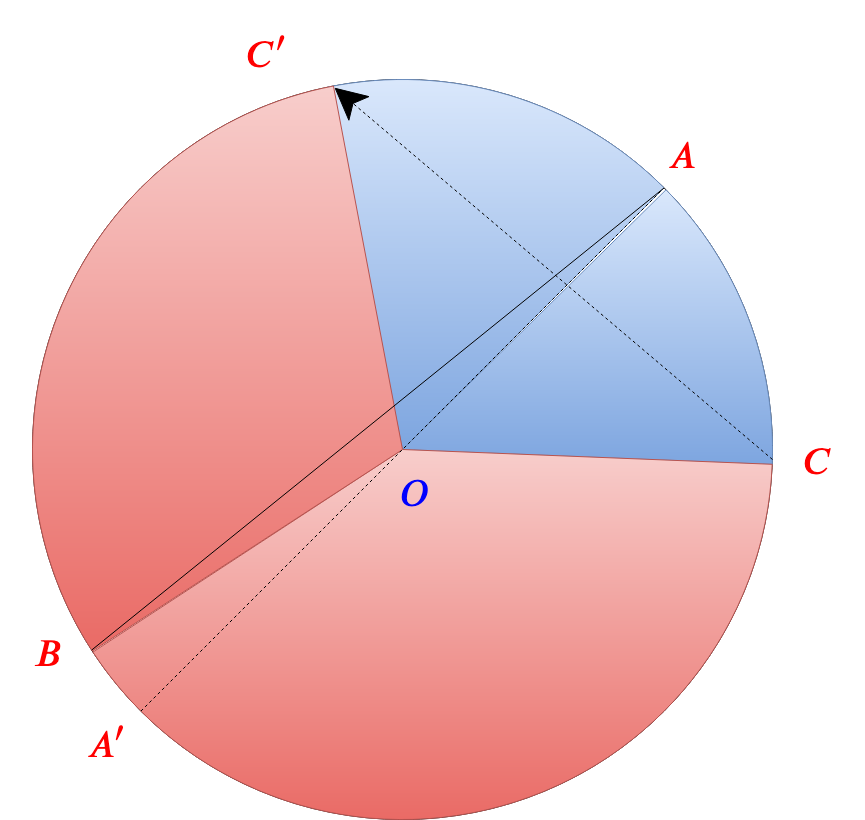
\includegraphics[scale=0.25]{Rund1.png}
\end{center}
\caption{}\label{Rund1}
\end{figure}
\item Пусть движение $M$ оставляет на месте ровно одну пару противоположных точек $A$ и $A'$ (см. рис. \ref{Rund1}).
Рассмотрим снова произвольную точку $C$ на окружности, отличную от $A$ и $A'$. И пусть $C'=M(C)$. Тогда $C\ne C'$ и $AC=AC'$. Отсюда следует, что $C'$ --- отражение точки $C$ относительно оси $AA'$. Следовательно, $M=S_\ph$, где $\ph$ --- угол наклона прямой $AA'$.
\item Пусть движение $M$ не оставляет на месте ни одной точки. Возьмем произвольную точку $A$ на окружности, и пусть $B=M(A)$ (по условию $B\ne A$). Обозначим за $\al$ угол дуги $AB$ (см. рис. \ref{Rund2}).

\begin{figure}[hbt!]
\begin{center}
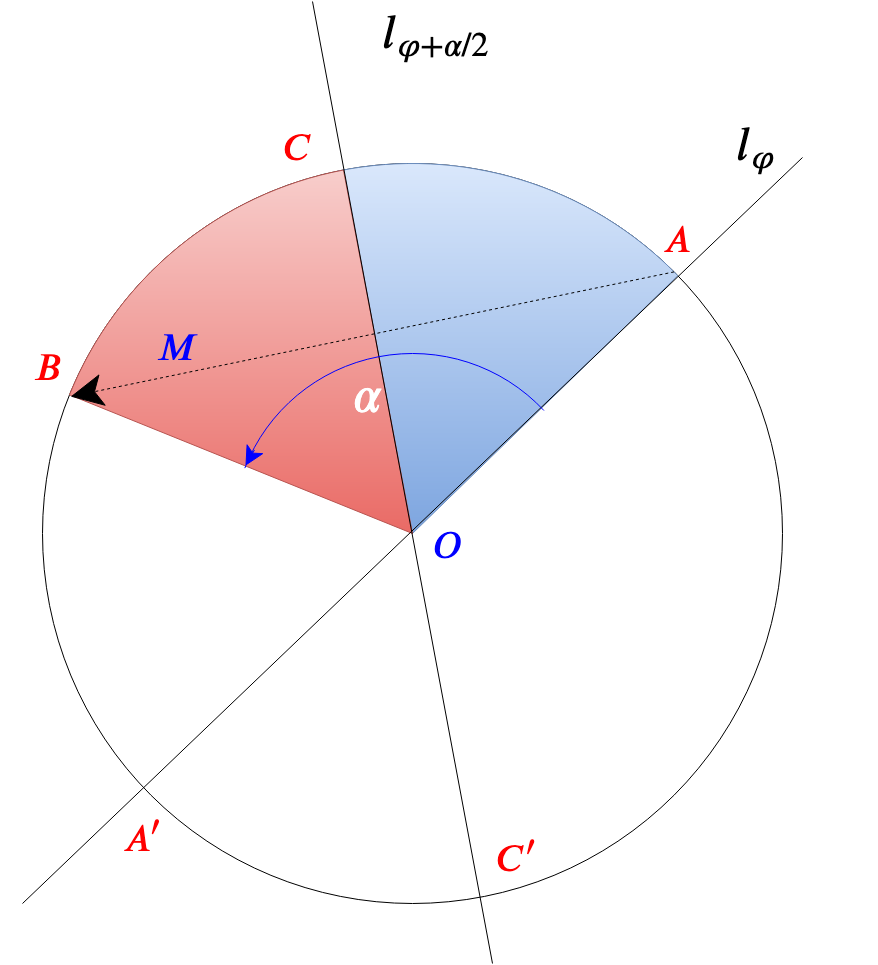
\includegraphics[scale=0.25]{Rund2.png}
\end{center}
\caption{}\label{Rund2}
\end{figure}
Тогда $R_{\al}^{-1}\circ M(A)=A$, т.е. $R_{\al}^{-1}\circ M$ оставляет на месте хотя бы одну точку $A$ (а точнее, пару противоположных точек $A$ и $A'$). Если оно оставляет на месте ровно одну пару точек $A$ и $A'$, то это некоторое отражение $S_\ph$ (на рис. \ref{Rund2} ось отражения обозначена за $l_\ph$), но тогда $M=R_\al\circ S_\ph=S_{\ph+\al/2}$ в силу второго равенства в \eqref{SRS}. Получается, что $M$ сохраняет точку $C$ на месте ($C$ есть середина дуги $AB$). Получаем противоречие с тем, что $M$ не оставляет на месте ни одной точки.

Остается вариант, что $R_{\al}^{-1}\circ M$ оставляет на месте как минимум две точки, не являющиеся противоположными, но тогда $R_{\al}^{-1}\circ M=\id$ (по доказанному ранее), откуда $M=R_\al\circ \id=R_\al$ --- поворот.

\item Таким образом, всякое движение окружности --- это либо поворот (в частности, $\id$), либо отражение относительно оси, проходящей через центр окружности (теорема Шаля).\index{Теорема!Шаля}
\item При этом любое движение окружности --- это либо одно отражение, либо композиция двух отражений.
\end{enumerate}
\subsection*{Задачи}
\begin{enumerate}
\item Центральная симметрия --- это какое движение?
\item Композицией каких отражений можно выразить центральную симметрию?
\item С помощью отражения относительно оси $Ox$ и вращений выразить отражение относительно оси $Oy$.
\end{enumerate}


\section{Наматывание прямой на окружность}

\lesson{Совмещаем вращение окружности и движение прямой: колесо на дороге. Шкала натуральных чисел соответствует полным оборотам колеса. Вращение в разные стороны соответствует положительным и отрицательным, т.е. целым числам. Определение разности чисел и отрицательной степени поворота окружности и сдвига. Концепция целых чисел как степеней сдвигов и поворотов без ограничений в ту или другую сторону.}

\begin{enumerate}
\item Совместим теперь окружность с прямой иным способом. Выделим на окружности точку $O$ и начнем ее обход (вращение) в положительном направлении.
\item Выше мы видели, что углы поворота, кратные $360^o$, т.е. полному обороту, соответствуют тождественному движению, т.е. приведут нас в точку отправления $O$.
\item Однако, если с точки зрения математического движения ничего не изменилось, физически мы проделали путь, равный длине окружности. Для удобства будем считать, что радиус окружности есть единичный вектор, так что ее длина равна $2\pi$, и с каждым полным оборотом мы будем <<наматывать>> расстояние $2\pi$.
\item Более общо, расстояние, пройденное по окружности единичного радиуса, когда этот радиус заметает угол $\al$, равно $\al(2\pi/360^o)$. Чтобы каждый раз не переводить единицы измерения радиуса в градусы и наоборот, углы также принято измерять в единицах длины --- радианах. А именно, \textit{угол в} 1 \textit{радиан соответствует повороту, при котором точка проделает по окружности путь, равный по длине радиусу данной окружности}. Нетрудно видеть, что в градусах 1 радиан будет иметь выражение $360^o/(2\pi)$ или $180^o/\pi \approx 57^o$.
\item В дальнейшем условимся все углы измерять в радианах, если не оговорено иное.
\item Известно, что число $\pi$ не соизмеримо с целыми числами (как уже отмечалось, этот факт является довольно сложной теоремой), так что поворот $R_1$ на 1 радиан ни в какой положительной степени не приведет нас снова в точку исхода $O$.
\item Зато поворот $R_{2\pi}$ в точности возвращает нас в точку отправления $O$.
\item При каждом таком повороте мы проделываем путь, равный углу поворота, т.е. $2\pi$ (радиус равен 1).
\item Следовательно, степени такого поворота $R_{2\pi}^n$ дадут прохождение пути длиной $2\pi n$.
\item Представим эту картину не с точки зрения жителей окружности, бегающих по замкнутой траектории, а с точки зрения жителей прямой, которая наматывается на окружность. С их точки зрения все выглядит несколько иначе и больше напоминает движение колеса по дорожному полотну: окружность катится по прямой и через равные промежутки касается точкой $O$ данной прямой.
\item Если при этом два друга --- один из мира окружности, второй из мира прямой, --- двигаются с одинаковой скоростью в одном направлении, то они могут синхронизироваться в точке касания окружности и прямой и разговаривать друг с другом, постоянно двигаясь каждый по своему объекту, но вместе.
\item Нужно заметить при этом, что если колесо вращается по часовой стрелке, т.е. в отрицательном направлении, то вдоль прямой оно движется направо, т.е. в положительном направлении. Но фокус в том, что житель окружности для синхронизации с жителем прямой должен идти навстречу вращению колеса, т.е. тоже в положительном направлении! Таким обраом, движения обоих друзей имеют одинаковый знак! На рис. \ref{RundLine} мы отметили синей стрелкой направление движения жителя окружности, а черной --- встречное вращение самой окружности.
\item Итак, колесо катится, два друга беседуют, точка $O$ то и дело, а именно, через каждые $2\pi$ метров соприкасается с прямой. Каждый раз, когда точка $O$ касается прямой, наш ученый друг из мира прямой ставит на ней отметины и считает их по порядку, т.е. приравнивает к степени совершенного поворота колеса: в начальный момент времени это был 0, затем 1 оборот, затем 2 оборота, и т.д.

\begin{figure}[hbt!]
\begin{center}
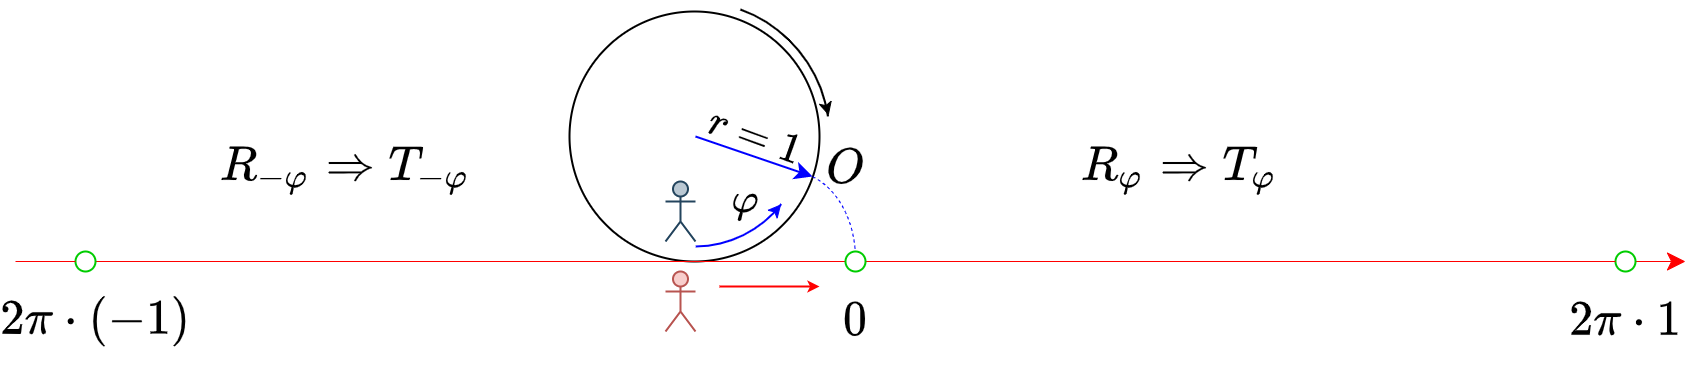
\includegraphics[scale=0.2]{RundLine.png}
\end{center}
\caption{}\label{RundLine}
\end{figure}

\item Что же мы видим на прямой? Мы видим не что иное как шкалу натуральных чисел, в точности соответствующую степеням вращений окружности. Число $2\pi$, фигурирующее как коэффициент, является не более чем единицей измерения. Кто-то измеряет в метрах, кто-то -- в ярдах, а мы измеряем в длинах единичной окружности.
\item Представим теперь, что в какой-то момент касания точки $O$ с прямой физика мира изменилась, и вращение начало осуществляться в обратную сторону!
\item Наши друзья-ученые при этом продолжат совместное путешествие, но только назад. Они пойдут отсчитывать уже проставленные отметки на прямой в убывающем порядке, пока не вренутся в точку 0. Но здесь процесс не остановится, и движение продолжится дальше.
\item Как все это записать на языке вращений и сдвигов?
\item Предположим, что сначала окружность повернулась на $n$ полных оборотов вперед, а затем на $m$ полных оборотов назад (см. рис. \ref{RundLine1}).
\item Мы получаем итоговое вращение, записываемое как $R_{2\pi n}\circ R_{2\pi m}^{-1}$.
\item А что мы имеем с точки зрения движения на прямой?
\item Сначала был произведен сдвиг $T_{2\pi n}$, затем сдвиг $T_{-2\pi m}$.
\item И мы видим, что индекс, определяющий итоговое вращение и итоговый сдвиг, --- один и тот же!
\item Причем, если $n>m$, то сдвиг жителя прямой будет вправо на расстояние $2\pi(n-m)$, а поворот жителя окружности будет положительным на угол $2\pi(n-m)$.
\item Если же $n<m$, то сдвиг жителя прямой будет влево на расстояние $2\pi(m-n)$, а поворот жителя окружности будет отрицательным (по часовой стрелке) на угол $2\pi(m-n)$.
\item Ранее мы уже договаривались, что перед векторами, направленными влево, будем ставить знак '-'. Так же мы будем поступать и с углами вращений в отрицательную сторону.
\item Соответственно, при $n<m$ мы будем иметь итоговый сдвиг на прямой $T_{-2\pi(m-n)}$ и итоговый поворот на окружности $R_{-2\pi(m-n)}$, которые также можно записать в виде степеней:
$$
T_{-2\pi(m-n)}=T_{2\pi}^{-(m-n)}\mbox{ и }R_{-2\pi(m-n)}=R_{2\pi}^{-(m-n)}.
$$

\begin{figure}[hbt!]
\begin{center}
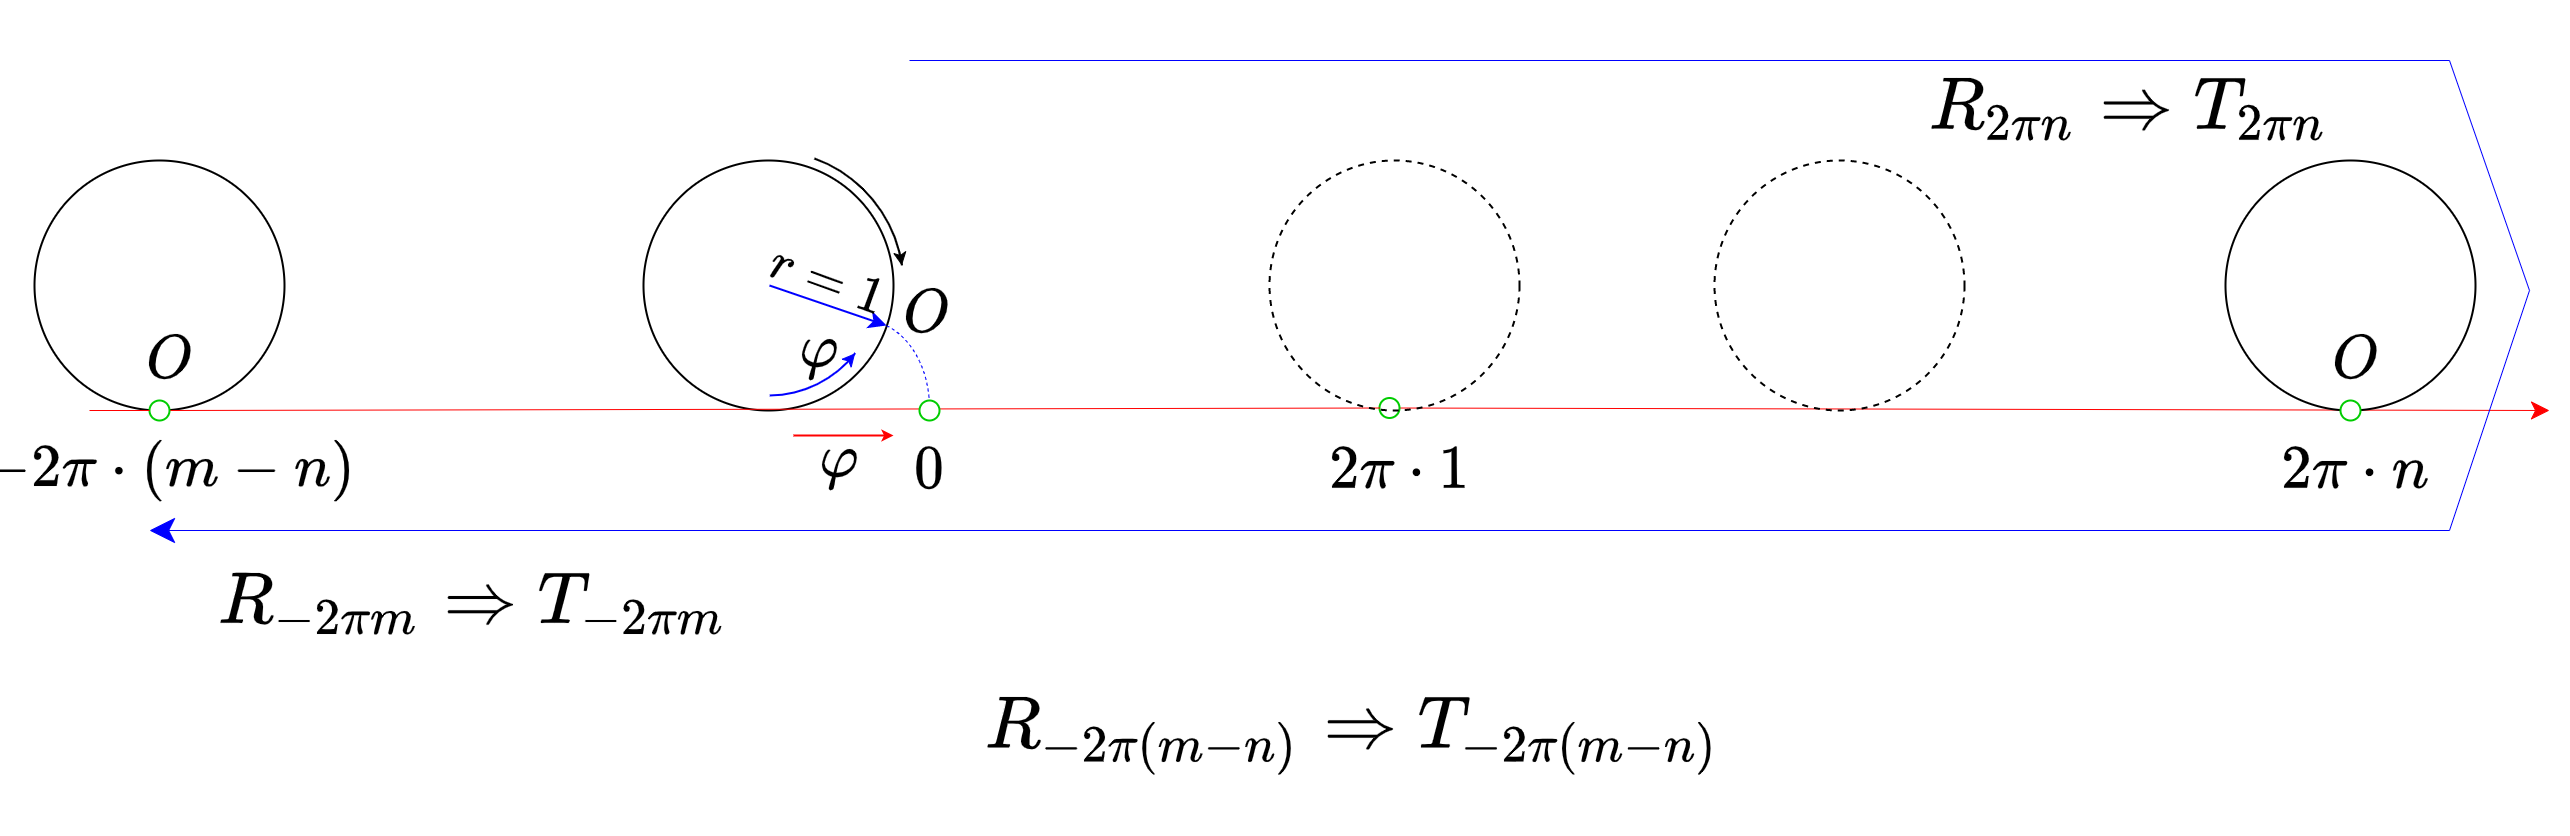
\includegraphics[scale=0.15]{RundLine1.png}
\end{center}
\caption{}\label{RundLine1}
\end{figure}

\item Осталось добавить маленький штрих к портрету, а именно: в случае $n<m$ под разностью $n-m$ будем понимать запись $-(m-n)$.
\item Тогда уже независимо от того, $n<m$, или $m<n$, или $n=m$, композиция поворотов и сдвигов сначала на $n$ вправо и затем на $m$ влево будет записываться одинаково:
$$
T_{2\pi(n-m)}=T_{2\pi}^{n-m}\mbox{ и }R_{2\pi(n-m)}=R_{2\pi}^{n-m}.
$$
\item В итоге мы приходим к тому, что называется \textbf{целыми числами}, включающими натуральные числа и отрицательные натуральные числа (при этом $-0=0$).
\item Сколько бы мы ни вращали окружность на $2\pi$ в ту или иную сторону с помощью поворота $R_{2\pi}$, мы совершаем поворот на целую степень полного оборота. При этом как бы мы ни катали окружность по прямой, точка $O$ будет ставить отметки в точках $2\pi k$, где $k$ --- целое число.
\end{enumerate}




\begin{comment}
\chapter{4. Целые числа и ОТА}
\end{comment}
\newchapter{Целые числа и ОТА}

\vrezka{
Это --- первая глава, где мы по-настоящему погружаемся в арифметику, используя тот понятийный аппарат, который был наработан в предыдущих главах. Здесь вводится обозначение множества целых чисел, дается строгое определение алгебраического понятия <<кольцо>>, обосновывается алгоритм Евклида.

Ключевым моментом является доказательство теоремы о том, что НОД двух чисел можно записать в виде их линейной комбинации с целыми коэффициентами. Этот факт выводится как непосредственно из алгоритма Евклида, так и с помощью сумм Минковского (что отсылает нас к главе 0).

Далее выводится основная теорема арифметики и некоторые ее следствия.
}

\section{Целые числа. Кольцо}

\lesson{Арифметика целых чисел на примере композиций сдвигов. Обобщение $\Z$ путем определения коммутативного кольца с единицей}

\begin{enumerate}\setlength{\itemsep}{1pt}
\item Итак, совмещение вращений со сдвигами дает нам полную свободу перемещений в положительном и отрицательном направлении. При этом с точки зрения окружности ничего не меняется --- происходит итоговое движение $\id$, а с точки зрения прямой --- происходит разметка точек с равным шагом. Ясно, что сам шаг при этом не имеет значения. Мы могли бы взять окружность радиуса $R$, и тогда шаг был бы равен $2\pi R$. В частности, можно взять радиус $R=1/2\pi$, и тогда точки на прямой расположатся с шагом 1.
\item Такую же картину можно получить, если взять все точки, получаемые из выделенной точки 0 степенями сдвига на единичный вектор, используя положительные и отрицательные, т.е. целые, степени.
\item Как видим, целые числа, как и натуральные, можно интерпретировать и как степени движений (и вообще любых преобразований, имеющих обратные), и как векторы сдвигов на прямой, а значит, к ним применимы определенные ранее операции сложения, вычитания и умножения. При этом результат умножения получает такой знак, который определяется из таблицы умножения знаков.
\item Множество всех целых чисел принято обозначать за $\Z$.\index{Целые числа}\index{Числа!целые}\index{Целые числа} Вместе с операциями сложения (вычитания) и умножения структура $(\Z,+,\cdot)$ называется \textbf{кольцом целых чисел}. Кольцо --- это структура, где можно складывать, вычитать и умножать (соблюдая обычные правила арифметики, см.ниже).
\item Понятие кольца является обогащением понятия группы, т.к. добавляется операция умножения. Всякое кольцо есть группа по операции сложения, т.е. кольцо можно считать частным случаем группы.
\item Ранее мы уже видели такие группы, как группа движений прямой, группа умножения знаков, группа композиций классов сдвигов и отражений, группа вращений окружности. Все они обладали одной операцией --- композицией, которая соответствовала сложению параметров сдвигов и вращений.
\item Кроме того, мы ввели такое понятие как кратность, заменяя тем самым многократное сложение умножением на целое число.
\item Кратность операций нельзя рассматривать как умножение сдвигов, вращений или отражений. Инае говоря, если у нас имеется запись $nT_v$, обозначающая $n$-кратный сдвиг на вектор $v$, то в этой записи слева стоит натуральное число, отвечающее за кратность операции сдвига, а справа --- собственно операция сдвига. В таком <<произведении>> множители принадлежат к разным понятиям (число и операция), а значит, запись $nT_v$ нельзя рассматривать как умножение операций или как умножение чисел, т.е. как бинарную операцию над множеством однородных объектов. Поэтому движения в общем случае образуют только лишь группу, но не кольцо. [Забегая вперед, мы можем сказать, что движения с операцией умножения на целое число образуют модуль над кольцом целых чисел.]
\item Однако уже сами кратности, как самостоятельные сущности, можно и складывать, и умножать. Например, если мы рассмотрим сдвиг $T_1$ и композицию его кратностей $T_1^n\circ T_1^m$, то получим тот же сдвиг, но в суммарной кратности $T_1^{n+m}$, где $n,m\in\Z$. Ничто не мешает нам рассмотреть кратность $m$ сдвига $T_1^n$, т.е. сдвиг $(T_1^n)^m$, а это уже будет не что иное, как сдвиг кратности $nm$, т.е. $T_1^{nm}$.
\item Иначе говоря, умножение на целых числах можно представить как кратности кратностей сдвигов!

\item Фиксируем понятие \textbf{кольца}.\index{Кольцо} Это --- множество $K$ с двумя бинарными операциями $+$ (плюс) и $\cdot$ (точка, <<умножить>>), которые подчинены следующим аксиомам:\label{Ring}
\begin{enumerate}[{\bf R}1]
\item $a,b\in K\Rightarrow a+b\in K, a\cdot b\in K$ (замкнутость операций);
\item $a,b,c\in K\Rightarrow (a+b)+c=a+(b+c), (a\cdot b)\cdot c = a\cdot (b\cdot c)$ (ассоциативность операций);
\item существует элемент $0\in K$ такой, что $a+0=0+a=a$ для всех $a\in K$ (аксиома нуля);
\item для всякого элемента $a\in K$ существует противоположный $-a$ такой, что $a+(-a)=0$ (аксиома противоположного элемента);
\item для всех $a,b,c\in K$ имеем $(a+b)\cdot c=(a\cdot c)+(b\cdot c)$, $c\cdot(a+b)=(c\cdot a)+(c\cdot b)$ (правая и левая дистрибутивность);
\item для всех $a,b\in K$ имеем $a+b=b+a$ (коммутативность сложения).
\end{enumerate}

Обычно изучаются \textbf{кольца с единицей},\index{Кольцо!с единицей} т.е. такие кольца, для которых
\begin{enumerate}[resume*]
\item существует элемент $1\in K$ такой, что $a\cdot 1=1\cdot a=a$ для всех $a\in K$ (аксиома единицы),
\end{enumerate}
а также \textbf{коммутативные кольца},\index{Кольцо!коммутативное} т.е. такие кольца, для которых
\begin{enumerate}[resume*]
\item для всех $a,b\in K$ имеем $a\cdot b=b\cdot a$ (коммутативность умножения).
\end{enumerate}

Иначе говоря, в коммутативном кольце с единицей можно складывать, вычитать и умножать по обычным правилам.

Отметим также, что иногда в определении кольца допускается ослабление требований, а именно, отмена требования ассоциативности умножения: $(ab)c = a(bc)$. Такие кольца называют неассоциативными. Но мы будем придерживаться классического определения термина <<кольцо>>, следуя в этом Кострикину \cite{Kostrikin}.
\end{enumerate}


\subsection*{Задачи}

\begin{enumerate}
\item *Установить коммутативность произвольного кольца, в котором каждый элемент $x$ удовлетворяет уравнению $x^2=x$.
\end{enumerate}

\section{Кузнечик НОД и алгоритм Евклида}\label{EVKL}

\lesson{Кузнечик с двумя целочисленными ногами. Формальный алгоритм Евклида, спуск по алгоритму до НОД, раскручивание алгоритма обратно: НОД как линейная комбинация исходных чисел}


\begin{enumerate}
\item Поработаем теперь непосредственно с целыми числами. Пусть у нас есть кузнечик, стоящий в точке 0, который умеет прыгать с шагом $a$ и с шагом $b$ в любую сторону. Числа $a,b$ --- натуральные.
\item Ясно, что он может попасть в любую точку вида $ka+mb$, где кратности $k,m$ --- целые. Можно ли проще описать, в какие точки он может попасть, а в какие --- нет?
\item Определим множество $m\Z$ как множество всех произведений $m$ на целые числа:
$$
m\Z = \{mk\mid k\in\Z\}.
$$
\item Пусть $d$ --- наименьшее положительное число, в которое кузнечик может попасть, т.е. оно имеет вид $d=ka+mb$ при некоторых $k,m$. Тогда он может попасть и в любое число вида $nd$, поскольку $nd=(nk)a+(nm)b$, где $n\in\Z$. Следовательно, кузнечик может попасть во все целые числа, кратные $d$ (множество $d\Z$).

\item Но в любые другие целые числа он не сможет попасть. Действительно, если он попадает в какое-то число $x$, лежащее между двумя соседними кратными $d$ числами, т.е. в число $x=nd+y$, где $0<y<d$, то тогда он может попасть в число $y$, т.е. остаток от деления $x$ на $d$. Для этого после попадания в точку $x$ ему нужно будет $n$ раз применить алгоритм перехода на расстояние $d$, только в обратном направлении (если, например, из нуля в точку $d$ он способен попасть, сделав $s$ шагов на $a$ и $t$ шагов на $b$, то для сдвига на $d$ влево ему надо сделать $-s$ шагов на $a$ и $-t$ шагов на $b$; повторив эти действия $n$ раз, кузнечик их точки $x=nd+y$ попадет в точку $y$).  Но $y<d$ и притом положительное, а это противоречит выбору числа $d$. Таким образом, кузнечик попадает во все точки $d\Z$, и только в эти точки!

\item Что такое $d$ на самом деле?

\item Заметим, что поскольку кузнечик можем прыгнуть в точки $a$ и $b$, а также, как мы только что показали, он прыгает только в точки, кратные $d$, то $a$ и $b$ сами кратны $d$, т.е. $d$ является их общим делителем.

С другой стороны, если какое-то $q>d$ также является общим делителем $a$ и $b$, то кузнечик прыгает только в точки, кратные $q$ (т.к. он попадает только в точки вида $ka+mb$), но тогда он окажется неспособным попасть в точку $d<q$, т.к. $d$ не кратно $q$.

Отсюда следует, что не существует делителя $a$ и $b$ большего, чем число $d$. Таким образом, $d$ --- наибольший общий делитель $a$ и $b$, $d=\gcd(a,b)$.

\hard{
\item Придем к тому же выводу, используя алгоритм Евклида (с отсечениями квадратов).\index{Алгоритм Евклида}
\item Пусть $a<b$. Вычтем из $b$ столько $a$, сколько сможем: $b=k_0a+r_1$, где $0\le r_1<a$. Далее, из $a$ вычитаем столько $r_1$, сколько сможем, если $r_1>0$. Получим $a=k_1r_1+r_2$, где $0\le r_2<r_1$. Снова, если $r_2>0$, вычитаем из $r_1$ столько $r_2$, сколько можем: $r_1=k_2r_2+r_3$, где $0\le r_3<r_2$. И так далее.
\item Видим, что всякий раз, если $r_i>0$, то мы приходим к $r_{i+1}<r_i$. Проблема в том, что это не может продолжаться бесконечно долго, т.к. от всякого натурального числа в сторону нуля можно спуститься за конечное число шагов (а ведь остатки у нас все положительные и целые!). Так что рано или поздно случится $r_{n+1}=0$, и на этом алгоритм Евклида остановится! Это значит, что прямоугольник $a\times b$ можно сложить квадратами $r_n\times r_n$.
\item Если теперь раскрутить равенства $r_{i-1}=k_ir_i+r_{i+1}$ в обратную сторону, то мы получим, во-первых, что $a$ и $b$ кратны $r_n$, и во-вторых, что $r_n=Ka+Mb$ при некоторых целых $K,M$. То есть, $r_n$ есть общий делитель исходных чисел $a$ и $b$, и наш кузнечик способен попасть в точку $r_n$ (а значит, и во все точки, ему кратные, т.е. в $r_n\Z$).
\item С другой стороны, если какое-то $q$ является общим делителем $a$ и $b$, то $q$ делит $r_1=b-k_0a$, делит $r_2=a-k_1r_1$, делит $r_3=r_1-k_2r_2$, и т.д., и, наконец, делит $r_n$. Стало быть, $q\le r_n$, и $r_n$ --- наибольшой общий делитель $a$ и $b$.
\item Итак, кузнечик способен попасть в НОД($a,b$), следовательно, $d\le\gcd(a,b)$. С другой стороны, выбор $d$ таков, что $d=ka+mb$ при некоторых целых $k,m$, но тогда всякий делитель $a$ и $b$ является и делителем $d$, в частности $\gcd(a,b)$ делит $d$, откуда $\gcd(a,b)\le d$. Таким образом, минимальный шаг, на который способен сдвинуться кузнечик, --- это наибольший общий делитель чисел $a$ и $b$. Поэтому кузнечика с ногами $a$ и $b$ можно назвать $\gcd(a,b)$. Он способен прыгнуть (в несколько прыжков) во ВСЕ точки, кратные $\gcd(a,b)$, и ТОЛЬКО в эти точки!}
\end{enumerate}
\subsection*{Задачи}
\begin{enumerate}
\item С помощью алгоритма Евклида найти $\gcd(2020,555)$.
\item Пусть в некоторой стране имеют хождение монеты достоинством только 14 и 23 тугрика. Продавец должен выдать сдачу покупателю в размере 1 тугрик. Считая, что у обоих имеется достаточное количество монет того и другого достоинства, указать способ, которым должен воспользоваться продавец для выдачи сдачи.
\item Докажите, что $m\Z$ --- подкольцо (без единицы) кольца $\Z$, т.е. в нем также можно складывать, вычитать и умножать, $m$ --- произвольное целое положительное число.
\end{enumerate}


\section{Простые числа и ОТА}\label{PrimeNumbers}

\lesson{Простые и взаимно простые числа. Простых чисел бесконечно много. Если простое делит $ab$, то делит по крайней мере одно из них. Доказательство ОТА классическое. Сумма делителей}

\begin{enumerate}
\item У кузнечика НОД может случиться уникальная ситуация, когда даже при достаточно больших числах $a$ и $b$ он способен прыгнуть в любое целое число! Это верно в том и только том случае, когда $\gcd(a,b)=1$. Тогда говорят, что $a$ и $b$ взаимно просты. Например, 125 и 63 взаимно просты (обозначение: $a\perp b$).\index{Числа!взаимно простые}
\item Натуральное число называется \textbf{простым}, если оно имеет ровно два делителя --- единицу и самого себя. \textit{Целое} число называется простым, если оно имеет ровно четыре делителя --- $\pm 1$ и самого себя со знаками $\pm$.\index{Числа!простые}
\item Если число $a$ простое, а число $b$ не кратно $a$, то $a$ и $b$ взаимно просты, т.к. $a$ имеет только делители $\pm 1$ и $\pm a$, но при этом $\pm a$ не делит $b$, значит, единственным положительным общим делителем $a$ и $b$ будет единица, т.е. $\gcd(a,b)=1$.
 Например, 101 --- простое, так что в паре с любым другим числом (кроме кратного 101) они будут взаимно просты, и наш кузнечик сможет прыгнуть в любую целую точку! Например, он умеет прыгать на 101 и 62, значит, он умеет прыгать в любое целое число!

\item Любое натуральное число можно представить как произведение степеней простых чисел. Действительно, 1 есть произведение нулевых степеней простых чисел, например, $2^0$. Предположим, что для всех чисел от 1 до $n$ утверждение о разложимости справедливо (внимание! индукция!) и рассмотрим число $n+1$. Оно либо уже простое, либо делится на число меньше $n$ и отличное от 1. Тогда $n+1=mk$, причем $m,k\le n$, а они есть произведение степеней простых по предположению индукции, но тогда и $n+1$ есть произведение степеней простых!
\item Простых чисел бесконечно много. Предположим, что это не так, и пронумеруем все простые числа:
$$
p_1=2,\;p_2=3,\;p_3=5,\;p_4=7,\;p_5=11,\;\dots,\;p_n
$$
Далее рассмотрим число $m=p_1p_2\dots p_n+1$. Это число не является простым, т.к. оно больше $p_n$. Тогда, по определению, оно должно быть кратным какому-то числу $d$, которое больше 1 и меньше $m$. По доказанному выше число $d$ можно представить как произведение степеней простых, причем как минимум одного простого в степени не меньше первой (иначе $d=1$), т.е. $d$ делится на какое-то простое число $p_k$ из данного ряда.

Тогда $m$ кратно числу $p_k$, т.е. $m=lp_k$. Отсюда следует, что
$$
1=m-p_1p_2\dots p_n = p_k(l-p_1\dots p_{k-1}p_{k+1}\dots p_n),
$$
т.е. единица кратна числу $p_k$. Противоерчие.

Следовательно, число $m$ не кратно никакому числу больше 1 и меньше $m$. Следовательно, наше предположение о том, что простых чисел конечный набор, --- ложно.

\item Если простое число $p$ делит произведение чисел $ab$, то оно по крайней мере делит одно из них. Доказательство: допустим, что $p$ не делит $a$, тогда $\gcd(p,a)=1$, но тогда, как мы уже видели выше, $1=kp+ma$ при некоторых целых $k,m$. Умножим это равенство на $b$: $b=kpb+mab$. Справа оба слагаемых делятся на $p$, значит, и $b$ делится на $p$.
\item Из этого свойства легко получить \textbf{основную теорему арифметики}: каждое натуральное число единственным образом представляется в виде произведения степеней простых чисел:\index{Теорема!основная теорема арифметики}\index{Основная теорема арифметики}
$$
n=p_1^{k_1}p_2^{k_2}\dots
$$
Набор степеней $k_1,k_2,\dots$ уникален для каждого числа $n$. Действительно, если бы было два разложения, то после сокращения на одинаковые сомножители мы бы получили равенство
$$
p_1^{k_1}p_2^{k_2}\dots p_m^{k_m} = q_1^{s_1}q_2^{s_2}\dots q_t^{s_t},
$$
где $\{p_1,\dots,p_m\}\cap\{q_1,\dots,q_t\}=\emptyset$.

Но каждое простое слева делит произведение чисел справа, значит, делит один из его множителей (по доказанному выше), а значит, совпадает с одним из $q_i$, что по предположению невозможно. Следовательно, разложение по степеням простых чисел единственно.
\item Здесь еще нужно сделать оговорку про $\Z$. Любое целое число также единственным образом раскладывается по степеням простых натуральных чисел, но с точностью до знака $\pm$ перед этим разложением.

\item Итак, возьмем произвольное натуральное число $n\ne 0$, перенумеруем все простые числа в порядке возрастания: $p_1=2, p_2=3, p_3=5, p_4=7,\dots$. В силу ОТА имеем единственное разложение
$$
n=p_1^{k_1}p_2^{k_2}\dots,
$$
где $k_1,k_2,\dots$ --- некоторые натуральные числа (в частности, нули).


Вопрос --- как с точки зрения разложений по степеням простых должны выглядеть делители числа $n$?

\item Пусть $m|n$ и $m>0$. Тогда $m=p_1^{t_1}p_2^{t_2}\dots$ при некоторых натуральных $t_1,t_2,\dots$
Кроме того, $n=qm$, где число $q$ также имеет разложение по степеням простых $q=p_1^{s_1}p_2^{s_2}\dots$

Отсюда получаем, что
$$
p_1^{k_1}p_2^{k_2}\dots = p_1^{s_1}p_2^{s_2}\dots\cdot p_1^{t_1}p_2^{t_2}\dots.
$$
Отметим, что все указанные произведения конечны, т.к. начиная с некоторого номера $j$ показатели степеней $k_j=t_j=s_j=0$ (иначе мы бы имели бесконечное произведение чисел, больших единицы). Поэтому мы можем воспользоваться коммутативностью и арифметическими свойствами степеней:
$$
p_1^{k_1}p_2^{k_2}\dots = p_1^{s_1+t_1}p_2^{s_2+t_2}\dots.
$$
Мы имеем два разложения одного и того же числа, а оно в силу ОТА единственно, так что
$$
k_1=s_1+t_1,\quad k_2=s_2+t_2,\quad\dots,
$$
откуда легко видеть, что $s_1\le k_1$, $s_2\le k_2$ и т.д. Иначе говоря, делители числа $n$ характеризуются тем, что их разложения по степеням простых включают те же самые простые числа, что и в разложении числа $n$, с равными и меньшими степенями.



\hard{

\item Отсюда, в частности, легко получить формулу для количества делителей числа $n$. Для этого нужно найти количество всех наборов $(s_1,s_2,\dots)$ таких, что $s_j\le k_j$ для каждого номера $j$. В силу ОТА выбор $s_j$ можно производить независимо друг от друга, не опасаясь получить на выходе одинаковые числа. Поэтому следует перемножить количество вариантов для каждой из степеней $s_j$. Например, для $s_1$ существует ровно $k_1+1$ вариант: $0,1,2,\dots,k_1$. Аналогично --- для остальных степеней.

Итак, количество делителей числа $n$ равно
$$
(k_1+1)(k_2+1)(k_3+1)\dots
$$
Это произведение конечное, т.к. начиная с некоторого номера $j$ степень $k_j=0$.

\item Наконец, получим формулу для функции $\si(n)$, равной сумме всех положительных делителей числа $n$.

Как мы уже видели выше, всякий делитель есть произведение вида $p_1^{s_1}p_2^{s_2}\dots$, где $s_j\le k_j$ для всех $j$. Иначе говоря, делители получаются как всевозможные произведения простых чисел, входящих в разложение числа $n$, во всех степенях, не превосходящих таковых в разложении числа $n$.

Для каждого $p_j$ и степени $k_j$ построим выражение $1+p_j+p_j^2+\dots+p_j^{k_j}$. Затем перемножим все такие выражения:
$$
(1+p_1+p_1^2+\dots+p_1^{k_1})(1+p_2+p_2^2+\dots+p_2^{k_2})\dots,
$$
в результате мы получим сумму всех возможных произведений вида $p_1^{s_1}p_2^{s_2}\dots$ с допустимыми значениями степеней. Все произведения, которые получаются после раскрытия скобок, различны в силу ОТА.

В свернутом виде функция $\si(n)$ записывается так:
$$
\si(n) = \prod_j(1+p_j+p_j^2+\dots+p_j^{k_j}).
$$
И это произведение также конечное, т.к. начиная с некоторого номера $j$ будем иметь $k_j=0$ и $(1+p_j+p_j^2+\dots+p_j^{k_j})=1$.

}

\end{enumerate}


\hard{

\lesson{Доказательство ОТА через операции Минковского. Доказываем, что если простое делит $ab$, то оно делит $a$ или $b$. Отсюда выводится ОТА так же, как выше.}

Основную теорему арифметики можно доказать разными способами. Покажем еще один способ, который использует множества и операции Минковского с этими множествами.


\begin{enumerate}[T1]
\item Пусть $P,Q\subseteq\Z$. Суммой и разностью по Минковскому называются, соответственно, множества:
$$
P\oplus Q=\{x+y\mid x\in P, y\in Q\},\quad P\ominus Q=\{x-y\mid x\in P, y\in Q\}.
$$
\item Множества вида $a\Z$ замкнуты относительно операций сложения и умножения (являются подкольцами кольца $\Z$), поэтому для любых $P,Q\subseteq a\Z$ и любых $k,n\in \Z$ имеет место вложение:
$$
kP\oplus nQ\subseteq a\Z.
$$
\item $a|b$ тогда и только тогда, когда $b\Z\subseteq a\Z$.

Действительно, если $a|b$, то $b=ka$. Если $x\in b\Z$, то $x=by=aky\in a\Z$.

Пусть $b\Z\subseteq a\Z$. Так как $b\in b\Z$, то $b\in a\Z$, т.е. $b=ka$ при некотором целом $k$, то есть $a|b$.

\item Решим вложение $P\ominus P\subseteq P$, где $P\subseteq \Z$.

1) Пустое множество удовлетворяет этому вложению.

2) Множество $P=\{0\}$ также удовлетворяет данному вложению.

3) Пусть $c\in P$ и $c\ne 0$. Тогда, во-первых, $0\in P$, поскольку $c-c\in P$ в силу вложения $P\ominus P\subseteq P$.

В-вторых, $-c\in P$, так как $-c=0-c$. Следовательно, вместе со всяким числом из $P$ ему также принадлежит противоположное по знаку число. А это значит, что в $P$ есть положительные числа.

Пусть $a=\min\{x\mid (x\in P)\land (x>0)\}$, т.е. наименьший положительный элемент $P$.
Нетрудно видеть, что $a\Z\subseteq P\ominus P$. Действительно, $a,0,-a\in P$ по доказанному. Тогда $a+a=a-(-a)$, $a+a+a = a+a-(-a)$ и т.д. --- все являются элементами $P\ominus P$. Аналогично --- для сумм вида $-a-a$, $-a-a-a$ и т.д. То есть, все числа вида $ka$, где $k\in\Z$, являются элементами множества $P\ominus P$. Откуда, в силу вложения $P\ominus P\subseteq P$ получаем, что $a\Z\subseteq P$.

Далее, если $P\setminus a\Z$ не пусто, то существует $x\in P\setminus a\Z$, причем $x=ka+d$, где $0<d<a$ (то есть $x$ не кратен $a$). Тогда $d=x-ka\in P\ominus P$, т.е. $d\in P$, что противоречит выбору $a$ как минимального положительного элемента $P$. Следовательно, $P\subseteq a\Z$, что вместе с предыдущим вложением дает $P=a\Z$.

Таким образом, если $P\ominus P\subseteq P$, то либо $P=\emptyset$, либо $P=a\Z$ при некотором целом $a$ (в том числе. при $a=0$ имеем $P=\{0\}$).

\item $a\Z\oplus b\Z=\gcd(a,b)\Z$.

Действительно, $P=a\Z\oplus b\Z$ удовлетворяет вложению $P\ominus P\subseteq P$, и значит, по свойству T4 $a\Z\oplus b\Z$ совпадает с множеством $c\Z$ при некотором $c$ (причем, если $a>0$ или $b>0$, то и $c>0$), т.е.
$$
a\Z\oplus b\Z=c\Z.
$$

Отсюда, с одной стороны, следует, что $a\Z,b\Z\subseteq c\Z$, откуда (свойство T3) $c|a$ и $c|b$. С другой стороны, если $d|a$ и $d|b$, то $a\Z,b\Z\subseteq d\Z$, откуда (свойство T2) $c\Z\subseteq d\Z$, откуда (свойство T3) $d|c$. То есть, любой делитель $a$ и $b$ делит число $c$, при этом $c$ также является делителем $a$ и $b$. Следовательно, $c=\gcd(a,b)$.

\item Если простое $p$ делит произведение $ab$, то $p|a$ или $p|b$ (или $p$ делит их обоих).

Предположим, что $p\not|a$, тогда $\gcd(p,a)=1$ и (по свойству T5) $p\Z\oplus a\Z=\Z$. Отсюда $1=kp+ma$ при некоторых целых $k,m$. Тогда $b=kbp+mab$, откуда следует, что $p|b$.

Если предположить, что $p\not|b$, то аналогично выводим соотношение $p|a$.
\item Отсюда, как уже отмечалось выше, легко выводится Основная теорема арифметики.
\end{enumerate}

}


\subsection*{Задачи}
\begin{enumerate}
\item Известно, что $n^2(m^2+1)(m+1)=9999$ при некоторых целых $n,m$. Найдите эти числа.
\item Произведение возрастов Машиных братьев равно 1664. Младший из братьев вдвое моложе старшего. Сколько у Маши братьев?
\item Пусть $a$ и $b$ --- натуральные числа, не делящиеся на 10, такие, что $ab=10000$. Чему равна их сумма?
\item В силу ОТА будем записывать положительное натуральное число $m$ как последовательность $\bar m$ степеней простых:
$$
m=p_0^{\al_0}p_1^{\al_1}\dots p_k^{\al_k}\ldots\iff \bar m=(\al_0,\al_1,\dots,\al_k,\dots),
$$
где $p_0<p_1<p_2<\dots$ --- все простые числа, начиная с 2.

Докажите, что если $\bar m=(\al_0,\al_1,\dots,\al_k,\dots)$ и $\bar n=(\be_0,\be_1,\dots,\be_k,\dots)$, то
\begin{align*}
\bar{nm} = & (\al_0+\be_0,\al_1+\be_1,\dots,\al_k+\be_k,\dots) \\
\bar{\gcd(n,m)} = & (\min(\al_0,\be_0),\min(\al_1,\be_1),\dots,\min(\al_k,\be_k),\dots), \\
\bar{\nok(n,m)} = & (\max(\al_0,\be_0),\max(\al_1,\be_1),\dots,\max(\al_k,\be_k),\dots).
\end{align*}

\item Докажите, что $\gcd(n,m)\nok(n,m)=nm$.

\item Докажите, что если $P\ominus P\subseteq P$, то выполняется равенство $P\ominus P=P$.
\item Докажите, что неравенство $P\ominus P\subseteq P$ определяет все подгруппы $\Z$ по сложению.
\item Найти $\si(p^k)$, где $p$ --- простое число, $k$ --- целое положительное, $\si$ --- сумма всех положительных делителей.
\item Натуральное число называется \textbf{совершенным},\index{Числа!совершенные} если сумма всех его делителей, меньших его, равно ему самому. Например, 6 и 28 --- совершенные числа. Докажите, что число $2^{n-1}(2^n-1)$ будет совершенным, если $2^n-1$ --- простое число.
\end{enumerate}


\begin{comment}
\chapter{5. Симметрии фигур}
\end{comment}
\newchapter{Симметрии фигур}

\vrezka{В этой главе мы снова возвращаемся к геометрии и занимаемся полным описанием групп движений правильных многоугольников, а заодно и всех конечных подгрупп движений окружности. В конце главы рассматривается нестандартный пример группы движений ромба и вводится определение четверной группы Клейна.
}

\section{Симметрии правильного треугольника}

\lesson{Полный разбор движений правильного треугольника, первое упоминание перестановок}

\begin{enumerate}
\item Вернемся на окружность и рассмотрим на ней вращение $R_{2\pi/3}$, т.е. на $120^o$.\index{Движения!треугольника}
\item Множество вращений $R^3=\{R_{2\pi/3},R_{2\pi/3}^2,R_{2\pi/3}^3\}$ образует циклическую группу. Видим, что
$$
R^3 = \{\id,R_{2\pi/3},R_{4\pi/3}\}.
$$
\item Зафиксируем точку $A$ на окружности и найдем ее образы при действии этой группы: $B=R_{2\pi/3}(A)$, $C=R_{4\pi/3}(A)$. Набор точек $\{A,B,C\}$ образует орбиту точки $A$ при действии группы $R^3$, а также представляет собой набор вершин правильного треугольника, вписанного в данную окружность.
\item Посмотрим теперь на треугольник $ABC$. Какие движения переводят его в себя? Очевидно, вращения из группы $R^3$, но также есть и отражения $S^3=\{S_A, S_B, S_C\}$ относительно осей, проходящих через центр окружности и вершины треугольника.
\item Можем проверить, что объединение $R^3\cup S^3$, состоящее из трех вращений и трех отражений, образует группу относительно операции композиции движений.
\item Выпишем полную таблицу композиций для этой группы:
\begin{table}[htb!]\begin{center}
\begin{tabular}{c||c|c|c||c|c|c|}
             & $\id$        & $R_{2\pi/3}$ & $R_{4\pi/3}$ & $S_A$        & $S_B$        & $S_C$  \\
\hline\hline
$\id$        & $\id$        & $R_{2\pi/3}$ & $R_{4\pi/3}$ & $S_A$        & $S_B$        & $S_C$  \\  \hline
$R_{2\pi/3}$ & $R_{2\pi/3}$ & $R_{4\pi/3}$ & $\id$        & $S_B$        & $S_C$        & $S_A$  \\  \hline
$R_{4\pi/3}$ & $R_{4\pi/3}$ & $\id$        & $R_{2\pi/3}$ & $S_C$        & $S_A$        & $S_B$  \\  \hline\hline
$S_A$        & $S_A$        & $S_C$        & $S_B$        & $\id$        & $R_{4\pi/3}$ & $R_{2\pi/3}$  \\  \hline
$S_B$        & $S_B$        & $S_A$        & $S_C$        & $R_{2\pi/3}$ & $\id$        & $R_{4\pi/3}$  \\  \hline
$S_C$        & $S_C$        & $S_B$        & $S_A$        & $R_{4\pi/3}$ & $R_{2\pi/3}$ & $\id$   \\  \hline
\end{tabular}
\end{center}\end{table}

\textbf{Важно!} Во всех таблицах умножения (сложения) порядок действий следующий: берется элемент из левого столбца, следом за ним пишется элемент из верхней строки, результат такой композиции пишется в соответствующую им ячейку. При этом последовательность применения операций обратная: сначала выполняется операция из верхней строки, затем к ее результату применяется операция из левого столбца.

Например, результат композиции $S_A\circ R_{4\pi/3}$ находится на строке $S_A$ в столбце $R_{4\pi/3}$ и равен $S_B$, поскольку композиция операций вычисляется \textbf{справа налево}. Если перепутать порядок действий, то результат будет другой, а именно, $S_C$, что неверно.

\item На примере этой группы мы можем заметить, во-первых, что в группе можно выделить подгруппу вращений (верхний левый квадрат $3\times 3$), во-вторых, что группа движений треугольника конечна и некоммутативна, поскольку ее таблица композиций несимметрична. Кроме того, в полном сооветствии с таблицей умножения классов $\R$ и $\S$ видим, что композиция вращений есть вращение, композиция вращения и отражения есть отражение, композиций двух отражений есть вращение.
\item Вопрос: есть ли еще какие-то движения окружности, переводящие правильный треугольник в себя?
\item Заметим, что при движении, переводящем треугольник в себя, вершины обязательно переходят в вершины.
Действительно, вершины правильного треугольника обладают тем свойством, что расстояние между любыми двумя из них является максимальным расстоянием внутри треугольника (какие две точки в треугольнике ни возьми --- расстояние между ними не может быть больше, чем длина стороны этого правильного треугольника). Движение сохраняет расстояния, следовательно, максимальные растояния также сохранятся, а значит, вершины могут перейти только в вершины.

Таким образом, преобразований правильного треугольника не может быть больше, чем всех возможных перестановок трех вершин:
$$
\begin{pmatrix}
A & B & C \\
A & B & C
\end{pmatrix},
\begin{pmatrix}
A & B & C \\
B & C & A
\end{pmatrix},
\begin{pmatrix}
A & B & C \\
C & A & B
\end{pmatrix},
$$
$$
\begin{pmatrix}
A & B & C \\
A & C & B
\end{pmatrix},
\begin{pmatrix}
A & B & C \\
C & B & A
\end{pmatrix},
\begin{pmatrix}
A & B & C \\
B & A & C
\end{pmatrix}.
$$
Нетрудно видеть, что эти перестановки в точности соответствуют преобразованиям $\id, R_{2\pi/3}, R_{4\pi/3}, S_A, S_B, S_C$. Так что данными преобразованиями исчерпываются все возможные движения, переводящие правильный треугольник в себя.
\end{enumerate}
\subsection*{Задачи}
\begin{enumerate}
\item Выписать все перестановки на 4 символах $A,B,C,D$.
\end{enumerate}



\section{Симметрии правильного многоугольника}



\lesson{Обобщаем на случай правильного многоугольника}

\begin{enumerate}
\item Рассмотрим еще один случай преобразований фигуры в себя. Пусть имеется правильный $n$-угольник. Тогда очевидными преобразованиями, сохраняющими форму и размеры фигуры, будут:\index{Движения!правильного многоугольника}
\begin{equation}\label{n-ugol}
R_{2\pi k/n},\quad S_k,\quad k=\overline{1,n}
\end{equation}
Обозначение $k=\overline{1,n}$ является краткой формой записи выражения $k\in\{1,\dots n\}$.
\item В случае четного $n$ в многоугольнике все вершины разбиваются на пары противоположных, лежащих на общей оси симметрии, поэтому имеется $n/2$ осей симметрии, проходящих через вершины, и $n/2$ осей, проходящих через середины строн. В случае нечетного $n$ на каждую вершину приходится своя ось симметрии.
\item Как и в случае треугольника, несложно показать, что этими $2n$ преобразованиями исчерпываются все движения, переводящие правильный многоугольник в себя. Действительно, движение многоугольника однозначно соответствует движению окружности, в котороую он вписан, поскольку все точки дуги окружности, соединяющей соседние вершины многоугольника, сохраняют свое положение относительно этих вершин при любом движении.

Следовательно, все движения правильного многоугольника, переводящие его в себя, есть частные случаи движений окружности, которые мы ранее изучили. По теореме Шаля такими движениями могут быть либо повороты относительно центра окружности, либо отражений относительно осей, проходящих через центр данной окружности. Остается понять, какие повороты и отражения сохраняют правильный многоугольник, т.е. переводят его в себя.

Достаточно очевидно, что вращение на любой угол, не кратный углу между соседними вершинами, т.е. углу $2\pi/n$, не сохранит многоугольник, т.к. не произойдет совмещение его вершин.

То же самое можно сказать и об отражениях относительно осей, угол которых, отложенный от оси, соединяющей две противоположные вершины, не кратен половине угла $2\pi/n$, т.е. углу $\pi/n$. При таких отражениях вершина, ближайшая к оси отражения, не достигнет никакой другой вершины многоугольника, а значит, многоуголник не перейдет в себя при таком преобразовании.

Итак, группа движений правильного $n$-угольника состоит ровно из $n$ поворотов и $n$ отражений, указанных в \eqref{n-ugol}.

\item Число $2n$ уже в случае квадрата ($2n=8$) сильно уступает количеству всех перестановок $n$ вершин, количество которых равно $n!$ (при $n=4$ оно равно $24$). С ростом $n$ группа движений правильного $n$-угольника содержит очень мало элементов по сравнению с группой всех перестановок $n$ точек.
\end{enumerate}
\subsection*{Задачи}
\begin{enumerate}
\item Составить полную таблицу композиций для группы движений правильного 4-угольника.
\item Выразить поворот на 90 градусов с помощью двух симметрий.
\end{enumerate}


\section{Подгруппы движений окружности}

\lesson{Переход от многоугольников к группам движений окружности. Первые определения теории групп: порядок элемента, циклическая группа. Полное описание конечных подгрупп движений окружности}

\begin{enumerate}
\item Правильные $n$-угольники дают приблизительное представление о подгруппах движений окружности. Приблизительное --- именно в том смысле, что движения $n$-угольников с любой наперед заданной точностью (при достаточно большом $n$) будут представлять движения окружности.\index{Подгруппа!движений окружности}
\item Вопрос: все ли конечные подгруппы движений окружности задаются движениями правильных $n$-угольников?
\item Ответ: да, но с оговоркой. Некоторые конечные подгруппы совпадают с группами движений $n$-угольников, другие же являются их собственными подгруппами.
\item Действительно, пусть $G$ --- некоторая подгруппа движений окружности, причем конечная, т.е.
$$
G=\{g_1,g_2,\dots,g_m\}.
$$
\item Возьмем произвольный элемент $g_k$ и рассмотрим множество всех его целых степеней:
$$
\langle g_k\rangle=\{\dots,g_k^{-1},g_k^0,g_k,g_k^2,\dots\}
$$
\item Данное множество, очевидно, является подгруппой группы $G$, а значит, конечно. Но тогда среди степеней $g_k$ точно есть два совпадающих значения: $g_k^s=g_k^t$ при $t\ne s$. Пусть для определенности $t>s$. Тогда, умножая равенство на $g_k^{-s}$, получаем $g_k^{t-s}=g_k^0=\id$. Иначе говоря, $g_k$ в некоторой положительной степени превращается в $\id$.
\item \textbf{Порядком элемента}\index{Порядок элемента группы} $g\in G$ называется минимальное целое положительное число $s$ такое, что $g^s=\id$. Как видим, для всякого $g_k\in G$ такой порядок существует.
\item При этом, как мы установили ранее, $g_k$ --- это либо поворот окружности, либо отражение относительно оси, проходящей через ее центр. В первом случае порядок может быть любым начиная с 1. В случае, когда порядок элемента $g_k$ равен 1, получаем, что $g_k=\id$, т.е. это --- поворот на нулевой угол (или угол $2\pi$). Во втором случае, очевидно, что порядок $g_k$ строго равен 2, т.к. отражение само себе обратно.
\item Если $g_k$ --- поворот и $s$ --- его порядок, то это поворот на угол $2\pi r/s$, где $r\perp s$. Действительно, с одной стороны, такой поворот в степени $s$ дает угол $2\pi r$, т.е. $\id$, с другой стороны, если бы $r$ и $s$ не были взаимно просты, то можно было бы сократить дробь $r/s$ на $\gcd(r,s)$, тем самым получив поворот на угол $2\pi r_1/s_1$, где $s_1<s$, а значит, число $s$ не было бы порядком поворота $g_k$.
\item Порядок элемента является одновременно и порядком подгруппы $\langle g_k\rangle$. Действительно, если $s$ --- порядок элемента $g_k$, то все $g_k$ в степенях меньше $s$ различны (иначе порядок оказался бы меньше $s$), а все бОльшие степени сводятся к меньшим сокращением на $g_k^s$. Так что в подгруппе $\langle g_k\rangle$ ровно $s$ элементов!
\item Конечная группа $\langle g_k\rangle$, порожденная степенями одного своего элемента, называется \textbf{циклической}.\index{Группа!циклическая} Это название вполне соответствует тому, что все элементы такой группы в нашем случае есть повороты окружности на определенный угол, нацело делящий $2\pi r$ при некотором целом $r>0$.

\item Итак, мы видим, что в $G$ есть подгруппы вида $\langle g_k\rangle$, которые либо тривиальны (состоят из одного элемента $\id$), либо соответствуют группам вращения правильных многоугольников (если $g_k$ --- поворот, причем здесь стоит оговориться, что при $g_k=R_\pi$ многоугольника как такового нет, это вырожденный двуугольник), либо соответствуют группам отражений вида $\{\id,S_\ph\}$ при некотором угле наклона $\ph$ оси отражения. 

\item Наша задача состоит в том, чтобы показать, что все эти подгруппы, а равно и сама группа $G$, есть подгруппы движений какого-то одного $n$-угольника.

\item Пусть $G'=\{g\in G\mid g\mbox{ --- поворот или }\id\}$. Ясно, что $G'$ --- подгруппа группы $G$. Предположим далее, что $G'\ne G$, т.е. в группе $G$ существует хотя бы одно отражение $h$. В этом случае, как мы видели ранее, все элементы произведения Минковского $hG'$ также являются отражениями. Предположим, что существует отражение $h'\in G\setminus (hG'\cup G')$. Ранее мы установили, что $hh'$ есть поворот, причем $hh'=g\in G'$, т.к. $hh'\in G$.
 Но тогда $h'=h^{-1}g=hg\in hG'$ (отражение обладает свойством $h=h^{-1}$), а это противоречит выбору $h'$.
\item Итак, если в группе $G$ есть отражения, то все они находятся в одном классе $hG'$, причем этот класс не зависит от выбора отражения $h$. Иначе говоря, все отражения порождены каким-то одним отражением и всеми поворотами. При этом может оказаться, что в группе $G$ есть только один поворот --- $\id$, а значит, там есть и только одно отражение.

\item Осталось разобраться с подгруппой $G'$ всех поворотов.
\item Возьмем из $G'$ самый маленький поворот $g_0$, т.е. тот, чей угол наименьший. Угол поворота $g_0$ обозначим через $x_0$, а порядок $g_0$ --- через $n$. Тогда $x_0n=2\pi r$ при некотором целом положительном $r$, взаимно простым с $n$.

Покажем, что на самом деле $r=1$. Так как $r\perp s_0$, то $r\al+n\be=1$ при некоторых целых $\al,\be$ (ранее мы получали это свойство из алгоритма Евклида). Тогда
$$
\frac{2\pi}{n} = \frac{2\pi r}{n}\al + 2\pi\be = x_0\al + 2\pi\be.
$$
Отсюда следует, что поворот $R_{2\pi/n}$ равен $g_0^\al$. Но так как $G'$ --- группа, то $g_0^\al\in G'$, и мы в множестве $G'$ находим поворот на угол $2\pi/n$, и если $r>1$, то это противоречит выбору $g_0$ (так как угол $x_0$ в этом случае будет больше, чем $2\pi/n$). Стало быть, $r=1$ и $x_0n=2\pi$.

\item Пусть $g$ --- произвольный поворот из $G'$ и его угол поворота равен $x>0$ (если угол поворота отрицательный, то можно рассмотреть $g^{-1}$, который также принадлежит $G'$). По условию $x\ge x_0$, а если $x$ не делится нацело на $x_0$, то имеет место представление
$$
x = kx_0+y,
$$
где $0<y<x_0$. Углу $y$ соответствует поворот $g'=g(g_0)^{-k}$, который, очевидно, принадлежит группе $G'$. Но тогда получается, что в группе $G'$ имеется поворот на угол $y<x_0$, что противоречит выбору $x_0$.

Следовательно, $y=0$ и $x$ кратно $x_0$. А это значит, что произвольный поворот $g\in G'$ является степенью минимального поворота из $G'$.

\item Таким образом, подгруппа $G'$ группы $G$ состоит из поворотов, являющихся степенями поворота $g_0$ --- того, у которого угол поворота наименьший среди поворотов группы $G'$ и равен $2\pi/n$! В частности, отсюда следует и то, что порядок самой группы $G'$ равен порядку этого наименьшего поворота $g_0$, т.е. числу $n$.
\item Итак, произвольная конечная группа движений окружности:
\begin{enumerate}[a)]
\item либо тривиальна, т.е. совпадает с $\{\id\}$,
\item либо является циклической группой поворотов $\langle g_0\rangle$, совпадающей с группой поворотов правильного $n$-угольника, где $n$ --- порядок этой группы (включая вырожденный случай 2-угольника),
\item либо является группой одного отражения $\{\id,S_\ph\}$,
\item либо есть объединение $\langle g_0\rangle\cup h\langle g_0\rangle$, где $h$ --- некоторое отражение того же самого правильного $n$-угольника.
\end{enumerate}
\item Наконец, заметим, что и тривиальная группа, и циклическая конечная группа поворотов порядка $n$, и группа одного отражения $\{\id,S_\ph\}$ (здесь важно отметить, что для согласования $S_\ph$ с многоугольником нужно, чтобы ось отражения проходила через вершину или середину строны многоугольника), и наиболее полная группа $\langle g_0\rangle\cup h\langle g_0\rangle$  --- все они являются подгруппами группы движений правильного $n$-угольника. Отсюда следует, что все конечные группы движений окружности являются подгруппами движений правильных многоугольников, лежащих на данной окружности.
\end{enumerate}

\subsection*{Задачи}
\begin{enumerate}
\item Доказать, что $\langle g_0\rangle\cap h\langle g_0\rangle = \emptyset$, т.е. конечная группа движений распадается на два непересекающихся класса, один из которых получается применением отражения ко второму.
\item Пусть $G$ --- коммутативная группа, $g\in G$ и $H$ --- подгруппа группы $G$. Доказать, что множество $gH$ равномощно множеству $H$, т.е. отображение $f(h)=gh$ разным $h$ ставит в соответствие разные значения, и при том все элементы $gH$ являются значениями отображения $f$.
\item Вывести из предыдущего утверждения \textbf{теорему Лагранжа}: порядок подгруппы делит порядок группы.\index{Теорема!Лагранжа о порядке группы}
\item Обобщить результат на некоммутативные группы.
\end{enumerate}

\section{Симметрии ромба, группа Клейна}

\lesson{Один не совсем правильный случай: ромб. На его примере впервые появляется четверная группа Клейна}

\begin{enumerate}
\item Рассмотрим ромб, не являющийся квадратом. У такого ромба группа движений существенно меньше, чем у квадрата.
\item Движения ромба состоят из:\index{Движения!ромба}
\begin{enumerate}[a)]
\item двух отражений: относительно его диагоналей, обозначим эти отражения за $S_1$ и $S_2$;
\item одного поворота: на угол $\pi$, обозначим этот поворот за $R$;
\item тождественного преобразования $\id$.
\end{enumerate}
\item Других движений ромба не существует. Докажем это.

Пронумеруем вершины ромба цифрами 1,2,3,4 (1 и 3 противоположны), причем будем считать, что диагональ $1--3$ --- наибольшая из двух. В этом случае расстояние между вершинами 1 и 3 является максимальным расстоянием между двумя точками в ромбе. Откуда следует, что диагональ $1--3$ при любом движении переходит только в саму себя. Если эта диагональ остается на месте при движении, то данное движение либо является $\id$, либо отражением относительно данной диагонали. Если эта диагональ переворачивается, то смотрим на вторую диагональ. Она может либо тоже остаться на месте, и тогда наше движение есть отражение относительно второй диагонали, либо тоже переворачивается, что соответствует повороту на угол $\pi$.

\item Таблица композиций группы движений ромба:
\begin{center}
\begin{tabular}{c||c|c|c|c|}
      & $\id$     & $R$   & $S_1$ & $S_2$ \\ \hline\hline
$\id$ & $\id$     & $R$   & $S_1$ & $S_2$ \\ \hline
$R$   & $R$       & $\id$ & $S_2$ & $S_1$ \\ \hline
$S_1$ & $S_1$     & $S_2$ & $\id$ & $R$ \\ \hline
$S_2$ & $S_2$     & $S_1$ & $R$   & $\id$ \\ \hline
\end{tabular}
\end{center}
\item Отличие данной группы от группы движений правильного $n$-угольника состоит в том, что группа ромба является коммутативной (абелевой).
\item Тем не менее, это не единственное ее отличие от групп движений правильного многоугольника.
Ведь в группе движений правильного многоугольника есть абелева подгруппа вращений. Например, группа вращений квадрата тоже имеет порядок 4. Но и тут мы находим отличие от группы движений ромба. Дело в том, что вращения квадрата есть степени одного поворота на прямой угол. То есть группа вращений квадрата --- циклическая. А если мы посмотрим на таблицу умножения группы движений ромба, то заметим, что степени вращения $R$ не дают ни одно из отражений, так же как и степени отражений не дают вращения. Это значит, что группа движений ромба не является циклической.
\item Тем не менее, такая группа не уникальна по своей природе. Ее ипостаси мы еще встретим при изучении вычетов и перестановок. С точностью до переобозначений элементов это будет все та же группа движений ромба. Вообще, если у двух групп получается одна и та же таблица композиций (умножения) при некотором соответствии элементов одной группы элементам другой, то такие группы называются \textbf{изоморфными}.\index{Изоморфизм групп} Общее название класса групп, изоморфных группе движений ромба, --- <<четвернаяя группа Клейна>>, и общее обозначение ее таково: $V_4$.\index{Группа!Клейна}
\end{enumerate}






\begin{comment}
\chapter{6. Линейные уравнения}
\end{comment}
\newchapter{Линейные уравнения}\label{LinearEqs}

\vrezka{
Основная задача данной главы --- дать полное описание решений линейных уравнений в целых числах. Попутно вводится уравнение прямой на координатной плоскости, хотя мы все еще подразумеаем, что работаем только с целыми числами.
}

\section{Уравнение прямой на плоскости}

\lesson{Получение уравнения прямой на плоскости, проходящей через $O$ и произвольную точку $(x_0,y_0)$. Прямая задается отношеением $y_0/x_0$. Уравнение прямой, не проходящей через $O$}

\begin{enumerate}
\item Рассмотрим плоскость с координатными осями $Ox$ и $Oy$. Что будет, если ее начать поворачивать? Во что переходит при этом ось $Ox$?
\item Поскольку вращение --- это движение, расстояние между точками сохраняется, и значит, никакие три точки, лежащие на прямой $Ox$, при повороте не могут перейти в точки, образующие невырожденный треугольник --- они снова лягут на прямую, причем в том же самом порядке. Стало быть, $Ox$ при вращении плоскости переходит в некоторую прямую.
\item Пусть центром вращения является точка $O=(0,0)$, и ось $Ox$ при вращении $R_\ph$ переходит в прямую $l$. Ясно, что $l$ такаже проходит через начало координат $O$, т.к. это --- стационарная точка вращения. Ранее (см. раздел \ref{CircleGroup}) мы построили таблицу композиций движений окружности, из которой видно, что вращения образуют подгруппу группы движений окружности, т.е. все движения вида $R_\ph$, где $0\le\ph<2\pi$, окружность переводят в окружность, сохраняя расстояния, при этом композиция вращений есть вращение, каждое вращение $R_\ph$ имеет обратное $R_{2\pi-\ph}$, кроме того, вращения коммутируют, т.е. образуют абелеву группу.
\item Фиксируем на $Ox$ точку $(1,0)$ и посмотрим, куда она переходит под действием всех возможных вращений с центром $O$, т.е. описанной выше группы вращений. Поскольку расстояние от центра вращения сохраняется, ясно, что эта точка остается на окружности радиуса 1. В то же время, выбирая произвольную точку на этой окружности, мы легко укажем угол $\ph$, на который нужно осуществить поворот плоскости относительно центра $O$, чтобы точка $(1,0)$ перешла в выбранную нами точку.
\item Итак, под действием группы вращений точка $(1,0)$ переходит во все точки единичной окружности. Аналогично, если мы выберем произвольную точку $(r,0)$ ($r>0$), она будет переходить во все точки окружности радиуса $r$ под действием группы вращений с центром в точке $O$.
\item В этом случае принято говорить, что группа вращений \textbf{действует} на плоскости, а множество всех значений, в которые она переводит выбранную точку, называют \textbf{орбитой} этой точки. В нашем примере орбитами являются коцентрические окружности с центром $O$.
\item Можно доказать, что орбиты образуют классы экивалентности, т.е. они попарно не пересекаются и в объединении дают всю область действия группы.
\item Фиксируем некоторое вращение $R_\ph$, и пусть точка $(1,0)$ при таком вращении перешла в точку $C=(x_0,y_0)$, лежащую на единичной окружности.
\item Возьмем произвольную точку $(r,0)$, где $r>0$, и проследим ее судьбу под действием того же вращения $R_\ph$. Пусть $A=(x,y)=R_\ph(r,0)$. Ясно, что точки $O,C,A$ лежат на одной прямой $l$.
\item Проведем вертикальные линии через абсциссы $x_0$ и $x$, а также горизонтальные линии через ординаты $y_0$ и $y$. Добавим новые точки пересечения $B$ и $D$ (см. рисунок \ref{linerotation}).

\begin{figure}[hbt!]
\begin{center}
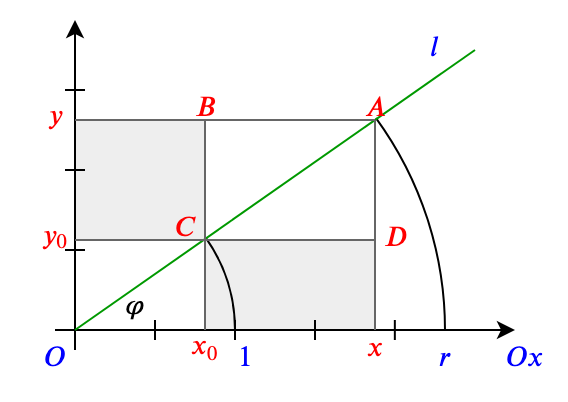
\includegraphics[scale=0.5]{linerotation.png}
\end{center}
\caption{}\label{linerotation}
\end{figure}
\item Видим, что треугольники $ABC$ и $ADC$ равны по трем сторонам, также равны треугольники $Oy_0C$ и $Ox_0C$, и треугольники $OyA$ и $OxA$. Отсюда легко установить равенство площадей $x_0(y-y_0)=y_0(x-x_0)$, откуда получаем
$$
xy_0-yx_0=0.
$$
\item Поскольку $(x,y)$ --- это произвольная точка прямой $OC$ (для отрицательного $r$ все доказывается аналогично),  данное уравнение есть уравнение прямой, проходящей через начало координат с углом наклона $\ph$.
\item Отметим, что точка $(x_0,y_0)$ полностью определяется углом поворота $\ph$, т.к. является образом точки $(1,0)$ при повороте на угол $\ph$. В то же время, произвольная точка на единичной окружности однозначно задает угол поворота в интервале от 0 до $2\pi$. Таким образом, задать поворот с центром $O$ и задать точку на единичной окружности --- суть одно и то же.
\item По определению $x_0=\cos\ph$ и $y_0=\sin\ph$, а отношение $y_0/x_0=\tg\ph$.
\item Кроме того, отношение $y_0/x_0$ также однозначно определяет угол поворота, но только в интервале от 0 до $\pi$.
\item Наконец, поворот прямой(!) на угол $\pi+\al$ --- это поворот на угол $\al$ с последующим отражением прямой $l$ относительно точки $O$. Но отражение прямой относительно своей же точки дает нам ту же самую прямую с тем же самым уравнением для ее точек! Таким образом, прямая, проходящая через начало координат, полностью определяется тангенсом угла наклона, т.е. отношением $y_0/x_0$.
\item Но раз все дело в отношении, стало быть, прямая задается любой точкой, координаты которой находятся в таком же соотношении, что и коодинаты точки $(x_0,y_0)$, лежащие на единичной окружности. Иначе говоря, одну и ту же прямую задают и все точки вида $(rx_0,ry_0)$, $(-rx_0,-ry_0)$, если коэффициент $r>0$. На рис. \ref{line} мы обозначили эти точки, соответственно, $C,A$ и $-C,-A$.
\begin{figure}[hbt!]
\begin{center}
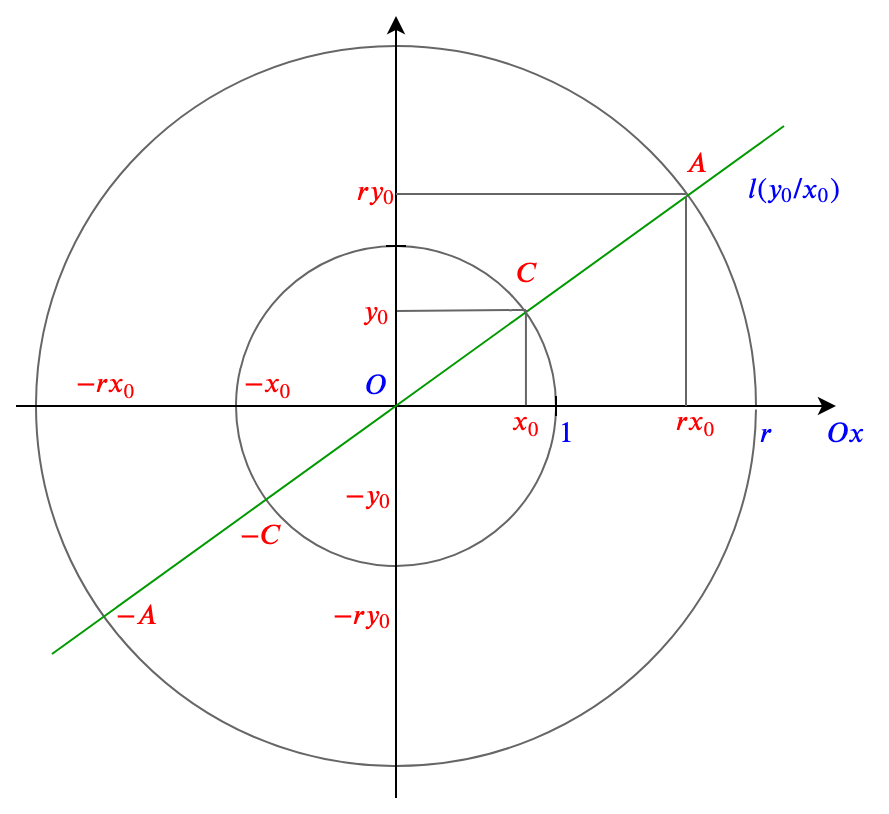
\includegraphics[scale=0.3]{line.png}
\end{center}
\caption{}\label{line}
\end{figure}
\item Этот вывод можно получить и более формально, просто глядя на уравнение прямой
$$
xy_0-yx_0=0.
$$
Ведь если мы домножим обе части уравнения на $r$, ничего не изменится!
$$
x(ry_0)-y(rx_0)=0.
$$
\item Что если прямая $l$ не проходит через центр координат $O$? В этом случае мы можем сдвинуть ее на некоторый вектор так, чтобы произвольно выбранная точка этой прямой перешла в точку $O$. Обозначим эту точку на прямой $l$ за $S=(\De x,\De y)$, а сдвиг, соответственно, осуществим на вектор $(-\De x,-\De y)$ (см. рис. \ref{lineshift}).
\begin{figure}[hbt!]
\begin{center}
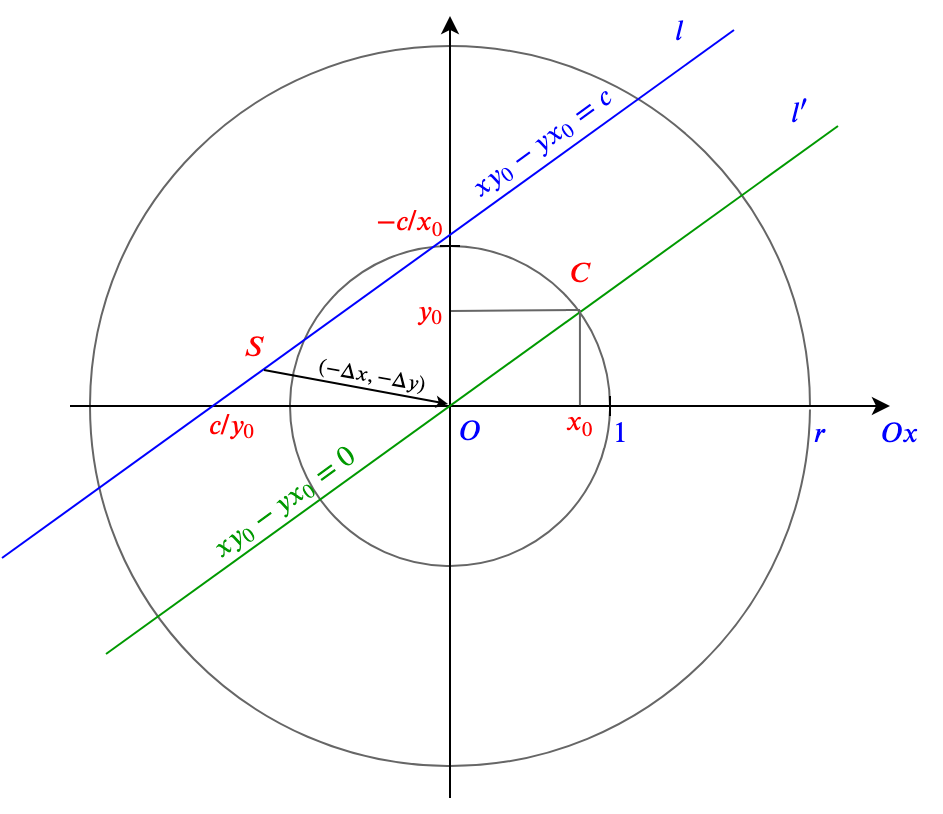
\includegraphics[scale=0.3]{lineshift.png}
\end{center}
\caption{}\label{lineshift}
\end{figure}
\item Тогда смещенные координаты $(x-\De x,y-\De y)$ уже будут пробегать прямую $l'$, проходящую через центр $O$, а ее уравнение нам известно:
$$
(x-\De x)y_0 - (y-\De y)x_0=0,
$$
или
\begin{equation}\label{lineq}
xy_0-yx_0=c,\quad\mbox{где } c= y_0\De x - x_0\De y.
\end{equation}
При этом коэффициенты $(x_0,y_0)$ все так же отвечают за наклон прямой $l$ и полностью определяются тангенсом угла наклона прямой $l$ относительно положительного направления $Ox$, т.е. отношением $y_0/x_0$.
\item Может показаться, что уравнение \eqref{lineq} сильно зависит от выбора точки $S$, поскольку свободный член $c$ зависит от координат точки $S$. Покажем, что это не так. Пусть $S'=(\De x',\De y')$ --- какая-то другая точка прямой $l$. В этом случае она удовлетворяет найденному уравнению, т.е.
$$
\De x'y_0-\De y'x_0=c,
$$
но уравнение, найденное с помощью точки $S'$, будет иметь вид
$$
xy_0-yx_0= y_0\De x' - x_0\De y',
$$
откуда из предыдущего получаем, что вновь
\begin{equation}\label{lineqmain}
xy_0-yx_0=c.
\end{equation}
Таким образом, для нахождения $c$ мы можем выбрать любую понравившуюся нам точку прямой $l'$, например, точку пересечения с одной из координатных осей.

\item Отметим также, что если взять произвольное уравнение вида \eqref{lineqmain}, т.е. с произвольно выбранными коэффициентами $x_0,y_0,c$, потребовав только, чотбы $x_0$ и $y_0$ одновременно не обращались в ноль, то оно однозначно определит прямую на плоскости. Эта прямая будет проходить через точки $(c/y_0,0)$ и $(-c/x_0)$ (см. рис. \ref{lineshift}), если $x_0\ne 0$ и $y_0\ne 0$. При $x_0=0$ мы получим более простое уравнение $xy_0=c$, которое определит вертикальную прямую, а при $y_0=0$ получаем уравнение $yx_0=-c$, которое определит горизонтальную прямую.

\item Таким образом, уравнение \eqref{lineqmain} является уравнением произвольной прямой\index{Уравнение!прямой} на координатной плоскости. Оно называется \textbf{линейным уравнением с двумя переменными}.
\item В случае, когда $x_0\ne 0$, уравнение прямой \eqref{lineqmain} также можно переписать в виде
$$
y = ax+b,\quad\mbox{где }a=\frac{y_0}{x_0},\; b=-\frac{c}{x_0}.
$$
\end{enumerate}
\subsection*{Задачи}

\begin{enumerate}
\item В какие точки переходят точки $(0,3)$ и $(4,0)$ при повороте на $90$ градусов? На $-90$ градусов?
\item Каков угол поворота, если точка $(a,b)$ перешла в точку $(-a,-b)$? В точку $(-b,a)$? В точку $(b,-a)$?
\item Чему равен тангенс угла наклона прямой $3x-5y=7$?
\item Какой угол наклона у прямой $y=-x+3$?
\item Доказать, что орбиты группы вращений с центром $O$ не пересекаются.
\item *Пусть $G$ --- подгруппа группы биекций некоторого множества $X$. Доказать, что орбиты группы $G$ в $X$ попарно не пересекаются и в объединении дают все множество $X$.
\end{enumerate}


\section{Линейные уравнения в целых числах}

\lesson{Определение линейного уравнения в целях числах, однородного уравнения. Сокращение на НОД. Общее решение неоднородного уравнения.}

\begin{enumerate}
\item Поскольку мы пока владеем аппаратом только целых чисел (множество $\Z$), рассмотрим задачу о нахождении всех целых точек плоскости, через которые проходит заданная прямая. Под целыми точками плоскости мы будем понимать такие точки, обе координаты которых принадлежат $\Z$.
\item В общем виде \textbf{линейное уравнение в целых числах} выглядит следующим образом:\index{Линейные уравнения в целых числах}\index{Уравнение!линейное в целых числах}
\begin{equation}\label{Zline}
ax-by=c,\quad\mbox{где коэффициенты } a,b,c\in\Z.
\end{equation}
Здесь мы сохранили форму уравнения \eqref{lineqmain} в продолжение предыдущей темы. В учебниках такое уравнение можно встретить в форме $ax+by+c=0$. Понятно, что если переобозначить коэффициенты, сменив знаки у $b$ и $c$, мы получим уравнение в форме \eqref{Zline}. Ниже будет понятно, почему такая форма удобнее для исследования данного уравнения.

\item Наша задача: найти все такие $x,y$, тоже целые, которые удовлетворяют уравнению \eqref{Zline}.
\item Сначала рассмотрим случай т.н. \textbf{однородного уравнения}:\index{Уравнение!линейное однородное}
$$
ax-by=0,
$$
т.е. мы отбрасываем ту часть уравнения, которая не зависит от переменных $x,y$.
\item Как мы уже знаем, данное уравнение задает прямую, проходящую через начало координат, а ее наклон определяется отношением $a/b$.
\item Для начала проверим, нельзя ли данное отношение упростить. Если числа $a,b$ имеют какой-то общий делитель, то разумно было бы на него сократить. И чтобы не проделывать это много раз, сократим их сразу на $\gcd(a,b)$. Множество решений от этого не изменится, а само уравнение по-прежнему останется однородным и целочисленным:
$$
\tilde ax-\tilde by=0,\quad\mbox{где } \tilde a=\frac{a}{\gcd(a,b)},\;\tilde b=\frac{b}{\gcd(a,b)}.
$$
\item Таким образом, мы приходим к уравнению со взаимно простыми коэффициентами $\tilde a$ и $\tilde b$.
\item Перепишем уравнение иначе: $\tilde ax=\tilde by$. Заметим, что все числа здесь --- целые. Причем $\tilde by$ делится на $\tilde a$. Но так как $\tilde a$ и $\tilde b$ взаимно просты, то $y$ делится на $\tilde a$. Это есть следствие того факта, который мы доказывали ранее в разделе \ref{PrimeNumbers}: если простое число $p$ делит произведение $ab$, то оно делит $a$ или $b$ (или их обоих). Поэтому если простое $p$ делит $\tilde a$, то оно делит $\tilde by$, но оно не может делить $\tilde b$, т.к. $\gcd(p,\tilde b)=1$, значит, оно делит $y$. Это значит, что все простые, составляющие число $\tilde a$, являются делителями $y$. В то же время, эти простые не входят в $\tilde b$, поскольку $\gcd(\tilde a,\tilde b)=1$. Поэтому, если $p^\al$ входит в разложение $\tilde a$, то $p^\al$ также делит $y$. Следовательно, $y$ делится на $\tilde a$, т.е. 
$$
y=k\tilde a
$$
при некотором целом $k$.
\item Симметрично рассуждая, получаем, что $x$ делится на $\tilde b$, т.е.
$$
x=t\tilde b
$$
при некотором целом $t$.
\item Подставим эти выражения в наше однородное уравнение:
$$
\tilde a(t\tilde b)=\tilde b(k\tilde a),
$$
откуда
$$
t=k,
$$
и больше никаких ограничений на выбор коэффициента $k$ мы не имеем.
\item Таким образом, решениями уравнения $\tilde ax-\tilde by=0$ являются
$$
\begin{cases}
x  =k\tilde b=kb/\gcd(a,b), \\
y  =k\tilde a=ka/\gcd(a,b),
\end{cases}
$$
где $k\in\Z$. Эти же $x$ и $y$ являются решениями исходного однородного уравнения $ax-by=0$.
\item Вернемся к неоднородному уравнению $ax-by=c$.
\item Для начала заметим, что если данное уравнение имеет решение в целых числах, то $ax-by$ делится на $\gcd(a,b)$, а значит, $c$ делится на $\gcd(a,b)$. Поэтому, если $c$ не делится на $\gcd(a,b)$, то решений точно нет, т.е. в таком случае прямая $ax-by=c$ проходит мимо всех целых точек плоскости!
\item Покажем, что в случае делимости $c$ на $\gcd(a,b)$ решения обязательно есть, и опишем все такие решения.
\item Пусть $c=d\gcd(a,b)$.
\item В разделе \ref{PrimeNumbers} мы установили, что $\gcd(a,b)$ является линейной комбинацией чисел $a$ и $b$, т.е. $\gcd(a,b) = an+bm'$ при некоторых целых $n$ и $m'$. Поскольку $m'$ --- целое, мы можем ввести новое обозначение $m=-m'$, откуда получим, что
$$
\gcd(a,b) = an-bm.
$$
\item Отсюда следует, что пара чисел $(dn,dm)$ удовлетворяет уравнению $ax-by=c$, поскольку
$adn-bdm=d\gcd(a,b)=c$.
\item Итак, представив $\gcd(a,b)$ в виде линейной комбинации $a$ и $b$, мы можем найти одно решение исходного уравнения.
\item Далее применим тот же прием, что и при изучении уравнений прямых --- сдвинем прямую $ax-by=c$ так, чтобы точка $(dn,dm)$ оказалась в начале координат. Для этого введем новые переменные
$$
\hat x = x-dn,\quad \hat y = y-dm.
$$
\item Тогда получаем, что $a\hat x-b\hat y = 0$. А такое уравнение мы уже решили выше, и его решением будет пара чисел $\hat x = kb/\gcd(a,b)$ и $\hat y = ka/\gcd(a,b)$, где $k$ --- любое целое число.
\item Собирая все вместе, находим общее решение исходного уравнения $ax-by=c$:
$$
\begin{cases}
x  = kb/\gcd(a,b) + dn, \\
y  = ka/\gcd(a,b) + dm,
\end{cases}
$$
где $d=c/\gcd(a,b)$, $n,m$ --- коэффициенты в представлении $\gcd(a,b)=an-bm$, $k$ --- это параметр решения, т.е. произвольное целое число.
\item Таким образом, решением линейного уравнения $ax-by=c$ в целых числах является сумма общего решения однородного уравнения $ax-by=0$ и какого-нибудь частного решения исходного уравнения.

\lesson{Получение НОД с помощью алгоритма Евклида. Метод цепных дробей}

\item Основной трудностью при поиске частного решения является нахождение коэффициентов $n$ и $m$ представления $\gcd(a,b)$.
\item Это представление можно найти с помощью алгоритам Евклида. Рассмотрим для примера уравнение
$$
18x-11y=2
$$
\item Следуя алгоритму Евклида, получаем выкладки:\index{Алгоритм Евклида}
\begin{align*}
18 = & 11\cdot {\color{red}1}+7,\\
   & 11 = 7\cdot {\color{red}1} + 4, \\
   & 7 = 4\cdot {\color{red}1} + 3, \\
   & 4 = 3\cdot {\color{red}1} + 1,
\end{align*}
где цветом выделены коэффициенты разложения. Последняя 1 --- это и есть $\gcd(18,11)$. Раскрутим алгоритм в обратную сторону:
\begin{align*}
1 & = 4-3 = 4 - (7-4) = 4\cdot {\color{red}2}-7 = (11-7)\cdot {\color{red}2}-7 =\\
  & = 11\cdot {\color{red}2}-7\cdot {\color{red}3} = 11\cdot {\color{red}2} - (18-11)\cdot {\color{red}3} =\\
  & = 11\cdot {\color{red}5} - 18\cdot {\color{red}3}.
\end{align*}
Таким образом, наши искомые числа $n=-3$, $m=-5$. Напомним, что мы ищем представление $\gcd(18,11)$ в виде $18n-11m$, исходя из чего нужно правильно выбирать знаки перед коэффициентами. Говоря проще,
$$
11\cdot{\color{red}5}-18\cdot{\color{red}3} = 1.
$$

Кроме того, $d=2$, т.к. $c=2$ и $\gcd(a,b)=1$. Откуда общее решение уравнения $18x-11y=2$ получаем в виде:
$$
\begin{cases}
x  =11k - 6, \\
y  =18k - 10,
\end{cases}
$$
где $k$ --- любое целое число. Проверим:
$$
18(11k - 6) - 11(18k - 10) = 198k-198k - 108 + 110 =2.
$$
\item Наконец, приведем еще один замечательный способ найти разложение НОД. Этот метод основан на представлении дробей в виде т.н. \textbf{цепных дробей}. Пусть дано уравнение
$$
112x-34y=16.
$$
\item Ищем приближение дроби $112/34$ следующим способом:\index{Цепная дробь}
$$
\frac{112}{34} = 3 + \frac{10}{34} = 3 + \frac{1}{3+\frac{4}{10}} = 
3 + \frac{1}{3 + \frac{1}{2+2/4}} = 3 + \frac{1}{3 + \frac{1}{2+1/2}}
$$
По сути дела, это --- другая запись выкладок алгоритма Евклида, поскольку мы каждый раз последовательно выделяем неполное частное предыдущих остатков.

Как только мы дошли до хвоста вида $1/k$, мы останавливаемся, отбрасываем этот хвост и сворачиваем дробь обратно, получая приближение исходной дроби:
$$
\frac{112}{34} \approx 3 + \frac{1}{3 + \frac{1}{2}} = \frac{23}{7}.
$$
Далее, перемножая накрест эти дроби, получаем представление для НОД:
$$
\gcd(112,34) = 112\cdot {\color{red}7} - 34\cdot {\color{red}23} = 2.
$$
Искомые коэффициенты: $n=7$, $m=23$. Общее решение уравнения, таким образом, получаем в виде
$$
\begin{cases}
x  = (34/2)k +  (16/2)\cdot 7, \\
y  = (112/2)k + (16/2)\cdot 23 ,
\end{cases}
$$
где $k$ --- любое целое число. Проверяем:
$$
112(17k +  8\cdot 7)-34(56k + 8\cdot 23) = 8(112\cdot 7- 34\cdot 23) = 16.
$$
\item Выше мы всюду рассматривали уравнения, в которых $x$ идет с положительным коэффициентом, а $y$ --- с отрицательным. Иначе говоря, прямая, заданная таким уравнением, имеет наклон <<вправо>> от вертикальной оси. Но уравнение может быть, например, таким
$$
5x+9y=1.
$$
Если мы хотим решать его по тем же формулам, то лучше перейти к новым переменным $\hat x=x$, $\hat y=-y$, и тогда мы получим уравнение
$$
5\hat x-9\hat y=1.
$$
Найдя его решения, мы просто меняем знак у $\hat y$, и получаем исходное уравнение.
\end{enumerate}

\subsection*{Задачи}

\begin{enumerate}
\item Найти линейное представление НОД с помощью алгоритма Евклида и методом цепных дробей:
$$
\gcd(5,9),\quad \gcd(18,15),\quad \gcd(225,81).
$$
\item Найти все решения линейного уравнения в целых числах или доказать что их нет:
\begin{enumerate}[a)]
\item $5x-9y=2$;
\item $225x+81y=18$;
\item $10x-18y=3$.
\end{enumerate}
\end{enumerate}


\begin{comment}
\chapter{7. Рациональность и соизмеримость}
\end{comment}
\newchapter[и соизмеримость]{Рациональность}\label{Fields}

\vrezka{
В этой главе мы начинаем выход за пределы целых чисел, и прежде всего займемся построением чисел рациональных. Кроме того, мы увидим, что одними рациональными числами нельзя ограничиваться, т.к. существуют несоиземеримые с ним числа вроде корня из 2.
}


\section{Построение рациональных чисел}

\lesson{Моделирование рациональных чисел с помощью прямых с целыми коэффициентами, проходящих через точку $O=(0,0)$. Наклон прямой --- это и есть рациональное число. Умножение на целое число. Сложение наклонов. Деление на целое число}

\begin{enumerate}
\item До сих пор мы часто оперировали дробями, хотя нигде их не определяли. Разве что упоминали отношение $y_0/x_0$ как некоторый параметр, определяющий угол наклона прямой на координатной плоскости в главе \ref{LinearEqs}.\index{Числа!рациональные}\index{Рациональные числа} Причем, для определения положения прямой важно именно отношение коэффициентов, а не их собственные значения.
\item Итак, рассмотрим прямую $l$, заданную уравнением $ax-by=0$, где $a,b$ --- целые числа. Прямая $l$ проходит через начало координат, т.е. точку $(0,0)$.
\item Для начала пусть $a=1$ и $b>1$. Легко видеть, что такая прямая проходит через точки $(0,0)$ и $(b,1)$ (см. рис. \ref{section}).
\begin{figure}[hbt!]
\begin{center}
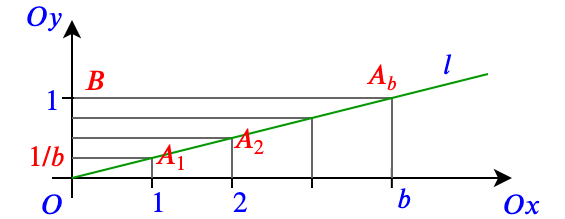
\includegraphics[scale=0.5]{section.png}
\end{center}
\caption{}\label{section}
\end{figure}
\item На прямой $l$ мы можем отметить точки $A_1, A_2, \dots, A_b$ в местах пересечения этой прямой с вертикальными прямыми, имеющими уравнения $x=1, x=2, \dots, x=b$, соответственно.
\item Теперь рассмотрим треугольник $OBA_b$, где точка $B=(0,1)$. В этом треугольнике мы можем провести линии, параллельные его горизонтальной стороне $BA_b$, которые отсекут на вертикальной стороне $OB$ нашего треугольника отрезки.
\item Эти отрезки будут иметь одинаковую длину (двукратное применение теоремы Фалеса), т.к. точки на прямой $l$ также расставлены с одинаковым шагом, что следует уже из выбора вертиклаьных секущих (они идут с шагом 1).
\item Итак, на вертикальной оси мы получили $b$ одинаковых отрезков, сумма длин которых равна 1.
\item Здесь можно снова обратиться к сюжету с синхронно шагающими товарищами, только теперь один из них шагает по прямой $Ox$ с шагом 1, а второй делает синхронные шаги по оси $Oy$ так, чтобы прямые, проведенные перпендикулярно их линиям движения всегда скрещивались на прямой $l$. Ясно, что длины шагов этих товарищей будут отличаться, и это отличие зависит от наклона прямой $l$.
\item Какова же длина шагов на оси $Oy$? Ответ: она равна одной $b$-ой части единицы. И эта часть записывается как дробь $1/b$. Собственно, отношение $1/b$, как мы видели ранее, является определяющим для прямой $l$. Оно характеризует величину \textbf{наклона} этой прямой.
\item Мы можем взять сумму нескольких таких частей (пройти несколько шагов). Например, $k$ ($k>0$) частей размера $1/b$ дают в сумме отрезок длины в $k$ раз больше, чем отрезок $1/b$. Такая часть записывается в виде дроби $k/b$.
\item Величину $k/b$ можно получить и другим способом. Возьмем теперь прямую $l'$, заданную уравнением $kx-by=0$ (см. рис. \ref{sectionkb}).
\begin{figure}[htb!]
\begin{center}
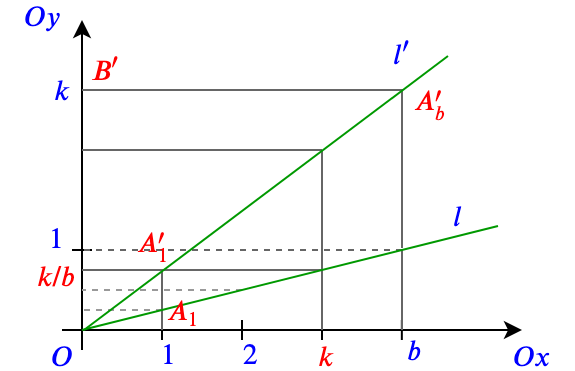
\includegraphics[scale=0.5]{sectionkb.png}
\end{center}
\caption{}\label{sectionkb}
\end{figure}
\item Эта прямая проходит через начало координат и точку $(b,k)$. Наклон этой прямой характеризуется отношением $k/b$.
\item Проделаем аналогичные предыдущему построения: проведем вертикальные линии с шагом 1, а затем горизонтальные линии от точек пересечения вертикальных с прямой $l'$, и посмотрим, какие отрезки у нас получатся на оси $Oy$.
\item Нетрудно видеть, что линия, соответствующая $x=k$, для прямой $l$ отсекает на оси $Oy$ метку, которую мы обозначили как $k/b$. Но ровно ту же самую метку покажет построение с помощью вертикальной линии $x=1$ и прямой $l'$. Почему? А очень просто: достаточно сравнить уравнения этих прямых
$$
l:\;x-by=0,\quad l':\;kx-by=0.
$$
Если в первом вместо $x$ подставить $k$, а во втором вместо $x$ подставить 1, то получим одно и то же значение $y$. Отсюда и совпадение меток.
\item Пользуясь сюжетом с двумя товарищами, мы можем сказать, что наклоны прямых $l$ и $l'$ задают разный масштаб шагов второго товарища относительно первого. А именно, наклон прямой $l'$ задает на оси $Oy$ шаг (или масштаб) в $k$ раз больше, чем наклон прямой $l$.

\item Получается, что наклон прямой, заданной уравнением $kx-by=0$, задает умножение на число $k$ того масштаба, который определяется наклоном прямой, заданной уравнением $x-by=0$.
\item Чтобы упростить терминологию, просто скажем, что наклон $k/b$ в $k$ раз круче наклона $1/b$.

\item Рассмотрим теперь прямую, заданную уравнением $ax-by=0$ с произвольными целыми коэффициентами $a$ и $b$ ($b\ne 0$). Ее наклон записывается в виде пропорции $a/b$. Мы можем провести построения, аналогичные предыдущему, и выяснить, что наклон прямой, заданной уравнением $(ka)x-by=0$, также окажется в $k$ раз круче наклона $a/b$, т.е. равным шагам на оси $Ox$ при тех же геометрических построениях на оси $Oy$ соответствуют шаги, которые в случае наклона $(ka)/b$ будут ровно в $k$ раз больше, чем шаги, соответствующие наклону $a/b$.

\item Таким образом, рассматривая наклоны прямых, заданные пропорцией их коэффициентов, как некие 
\textit{новые объекты}, мы можем ввести понятие умножения наклона на целое число. Если у нас есть наклон $a/b$ прямой, заданной уравнением $ax-by=0$, то результатом его умножения на число $k$ является наклон $(ka)/b$ прямой, заданной уравнением $kax-by=0$. Обозначая умножение числа на наклон точкой или пустым символом, запишем данное утверждение следующим равенством:
$$
k\cdot(a/b) = (ka)/b,
$$
причем теперь мы не будем ограничиваться только положительным $k$, считая его произвольным целым числом (в частности, нулем, при котором наклон станет нулевым, а прямая горизонтальной, и все шаги на оси $Oy$ схлопнутся в одну точку --- второй товарищ буде топтаться на месте, пока первый шагает вперед или назад).
\item Далее, число $k$ --- целое, стало быть, оно является суммой единиц (или минус единиц) в количестве $|k|$. А это значит, что умножение на $k$ можно представить как многократное сложение:
$$
k\cdot(a/b) = \underbrace{a/b + a/b + \dots + a/b}_{k}
$$
для положительного $k$ и
$$
k\cdot(a/b) = \underbrace{(-a)/b + (-a)/b + \dots + (-a)/b}_{-k}
$$
--- для отрицательного. Умножение на $-1$ мы просто ввели по определению.

\item Далее, мы можем в этих суммах расставлять скобки как угодно и сворачивать внутри них сложение обратно в умножение, получая тем самым аддитивное свойство умножения наклона целое число. Если $k=k_1+k_2$, то
$$
k\cdot(a/b) = k_1\cdot(a/b) + k_2\cdot(a/b).
$$
Заметим, что это на самом деле закон дистрибутивности, являющийся одной из аксиом кольца и связывающий сложение с умножением.

\item Идем дальше. По уже установленным правилам оперирования с наклонами, нетрудно видеть, что
$$
k_1\cdot(a/b) = (k_1a)/b,\quad k_2\cdot(a/b) = (k_2a)/b,\quad k\cdot(a/b) = (ka)/b,
$$
откуда получаем, что
$$
(k_1a)/b + (k_2a)/b = (ka)/b,
$$
а поскольку произведения $k_1a, k_2a, ka$ --- произвольные целые числа, мы получаем правило сложения наклонов
$$
a_1/b + a_2/b = (a_1+a_2)/b.
$$
\textbf{Важно:} при сложении наклонов коэффициент $b$, т.е. знаменатель отношения и одновременно коэффициент перед переменной $y$ в уравнении соответствующей прямой, должен быть одинаковым у обоих слагаемых!
Только в этом случае мы получаем согласование операций сложения и умножения.

\item Сложение наклонов прямых можно интерпретировать графически как сложение площадей прямоугольников с основанием $b$ и высотой $a_1$ и $a_2$. В результате получается прямоугольник с тем же основанием $b$ и высотой $a_1+a_2$. При этом прямые всегда проходят через точку $(0,0)$ и через правый верхний угол прямоугольников (см. рис. \ref{linesum}).
\begin{figure}
\begin{center}
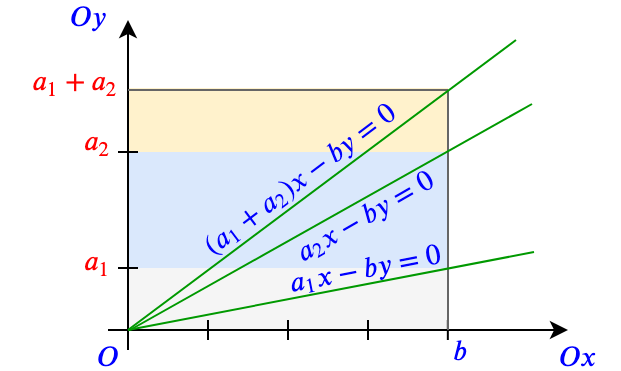
\includegraphics[scale=0.5]{linesum.png}
\end{center}
\caption{}\label{linesum}
\end{figure}
С помощью этой же картинки можно представить себе и умножение наклона прямой на целое число $k$. Для этого нужно растиражировать соответствующий этому наклону прямой прямоугольник вверх $k$ раз.

\item На самом же деле операции сложения, вычитания и умножения на целое число, производимые с коэффициентом перед $x$ уравнения прямой, в точности повторяют таковые операции над целыми числами (поскольку это и есть целые числа!) и, соответственно, подчиняются всем аксиомам кольца целых чисел (дистрибутивный закон мы уже видели, а коммутативность сложения и умножения, существование нуля и единицы и обратных --- все это наследие кольца $\Z$). [А вот и более умный термин для тех, кто собирается идти в математику глубоко: \textit{наклоны прямых с общим основанием $b$ образуют модуль над кольцом} $\Z$.]
\item Поэтому все наклоны вида $a/b$, $a,b\in\Z$, при фиксированном $b\ne 0$ с определенныими выше операциями сложения и умножения \textit{образуют кольцо} (изоморфное кольцу целых чисел). 
\item Заметим теперь, что уравнение $x-by=0$ прямой $l$ можно переписать иначе: $kx-(bk)y=0$. Чем оно отличается от уравнения $kx-by=0$ прямой $l'$? Очевидно, тем, что перед $y$ появился коэффициент $k$. А теперь вспомним, что прямая $l'$ задает наклон в $k$ раз больше, чем прямая $l$. И это значит, что если мы хотим разделить наклон прямой $l'$ на $k$, то мы должны умножить на $k$ ее коэффициент перед $y$.

\item Итак, если мы хотим умножить наклон прямой с уравнением $ax-by=0$ на целое число, то мы умножаем на это число коэффициент перед $x$ (прямая становится более крутой), а если мы хотим разделить наклон прямой на целое число, то мы умножаем на это число коэффициент перед $y$ (прямая становится более пологой):
$$
k(a/b)=(ka/b),\quad (a/b)/k = a/(bk).
$$




\lesson{Определение умножения наклонов прямых. Графическая иллюстрация умножения. Поле рациональных чисел. Почему нельзя делить на ноль. Аксиомы поля}


\item Делаем следующий шаг: умножение двух наклонов. На самом деле, наклон любой прямой вида $ax-by=0$ мы можем выразить через композицию ранее определенных операций --- умножения на целое число и деления на целое число:
$$
a/b = a\cdot(1/1)/b,
$$
откуда видим, что прямая $x-y=0$ (соответствующая пропорции $1/1$) имеет наклон $45^o$ и в операциях умножения может опускаться точно так же, как обычная единица. Таким образом, умножение наклонов прямых выглядит следующим образом
\begin{gather*}
(a_1/b_1)\cdot(a_2/b_2) = \\
= a_1(1/b_1)\cdot (a_2/1)/b_2 = a_1(a_2/b_1)b_2 = (a_1a_2)/(b_1b_2).
\end{gather*}

\item Отсюда нетрудно получить и процедуру деления наклонов прямых друг на друга, решив уравнение:
$$
(a_1/b_1) = (a_2/b_2)(c/d),
$$
т.е.
$$
(a_1/b_1) = (a_2c)/(b_2d),
$$
и эти наклоны задают одну и ту же прямую двумя разными способами. Умножим наклон в левой части равенства на единичный наклон $(1/1)$, представлнный пропорцией $(a_2b_2)/(a_2b_2)$, получим
$$
(a_1a_2b_2)/(a_2b_1b_2) = (a_2c)/(b_2d),
$$
откуда видно, что можно выбрать следующее решение
$$
c = a_1b_2,\quad d = a_2b_1,
$$
а также любое ему пропорциональное в любое целое число раз (кроме нуля). Таким образом,

$$
(a_1/b_1)/(a_2/b_2) = (a_1b_2)/(a_2b_1).
$$

\item Наконец, чтобы научиться складывать произвольные наклоны прямых, мы должны уметь сводить сложение произвольных прямых к сложению прямых с одинаковым коэффициентом перед $y$, т.к. сложение мы определили выше только для данного случая.
\item Но и это не проблема:
\begin{gather*}
(a_1/b_1)+(a_2/b_2) = (a_1b_2)(b_1b_2) + (a_2b_1)/(b_1b_2) = \\
= (a_1b_2+a_2b_1)/(b_1b_2).
\end{gather*}

\item Следующая картинка \ref{linear} показывает <<арифметику наклонов>> с произвольными параметрами.
\begin{figure}[htb!]
\begin{center}
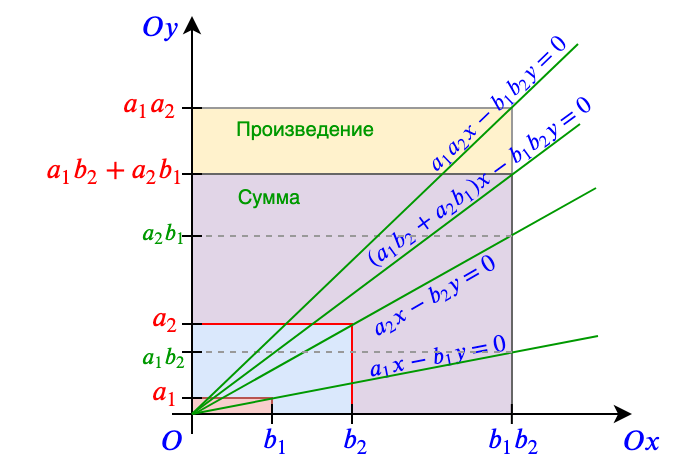
\includegraphics[scale=0.5]{linear.png}
\end{center}
\caption{}\label{linear}
\end{figure}
Здесь маленькие прямоугольники соответствуют исходным прямым с уравнениями $a_1x-b_1y=0$ и $a_2x-b_2y=0$, пунктиром отмечены приведенные к общему основанию $b_1b_2$ прямоугольники, большой темный прямоугольник соответствует их сумме (буквально однин приставлен сверху к другому), большой светлый прямоугольник --- произведению (помножены основания и помножены высоты). На рисунке не нанесен масштаб (т.е. не указаны единицы на обеих осях). Дело в том, что в зависимости от выбора масшштаба положение чисел на оси $Oy$ может иметь различный порядок. Выбранное расположение нужно считать условным.

\item В целом картина представления рациональных чисел с помощью прямых с целочисленными коэффициентами выглядит следующим образом (рис. \ref{ratio}):\index{Рациональные числа}\index{Числа!рациональные}
\begin{figure}[htb!]
\begin{center}
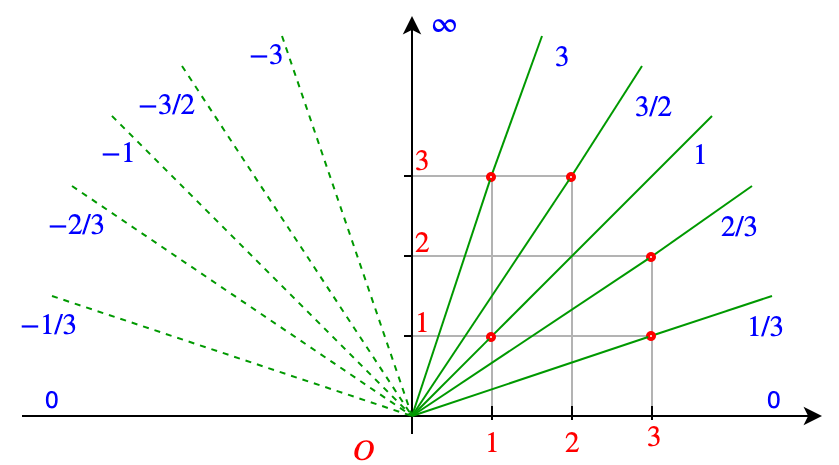
\includegraphics[scale=0.4]{ratio.png}
\end{center}
\caption{}\label{ratio}
\end{figure}
\item Итак, имея только множество целых чисел $\Z$, мы построили на плоскости всевозможные прямые, заданные линейными уравнениями с целыми коэффициентами, научились складывать, вычитать, умножать и делить их наклоны. Тем самым, мы построили новую алгебраическую структуру, которая называется \textbf{полем рациональных чисел} и обозначается $\Q$.

\item На самом деле, в нашем построении есть еще и такая прямая, которая соответствует бесконечности. Это прямая, заданная уравнением $x=0$. Ее наклон можно записать как $1/0$ (хотя, строго говоря, вместо единицы можно подставить любое отличное от нуля целое число) или просто $\infty$. Нулевой наклон определяется уравнением $y=0$ и записывается пропорцией $0/1$ или просто $0$. В полном соответствии с установленными правилами, мы можем заметить, что если $a\ne 0 \ne b$, то
\begin{gather*}
(a/b)(0/1)=0/1=0,\;(a/b)(1/0)=1/0=\infty,\\ 
(a/b)/(0/1)=1/0=\infty,\;(a/b)/(1/0)=0/1=0,
\end{gather*}
при $a\ne 0\ne b$,
т.е. деление на ноль дает бесконечность, а деление на бесконечность дает ноль для любых ненулевых конечных наклонов прямых.

\item Но тут кроется проблема: $(1/0)\cdot(0/1)=0/0$, что соответствует уравнению $0x-0y=0$. Такое уравнение не задает прямую, его решением является вся плоскость! Проще говоря, при умножении $0\cdot\infty$ может получиться любое число!
\item Поэтому при определении поля бесконечный элемент не постулируется и, соответственно, деление на ноль не разрешено.
\item Поле рациональных чисел является представителем огромного количества различных полей, известных в математике. Как и кольцо, общее алгеьраическое понятие поля задается списком аксиом, накладывающих некоторые дополнительные ограничения на кольцо. А именно --- в поле операция умножения должна быьт коммутативной и, кроме того, в поле разрешается делить на любой ненулевой элемент.
\item Приведем полный формальный список аксиом поля.\index{Поле} Множество $F$ с операциями $+$ и $\cdot$ называется \textbf{полем}, если:\index{Поле!аксиомы поля}\label{FildAxiom}
\begin{enumerate}[{\bf F}1]
\item $a,b\in F\Rightarrow a+b\in F, a\cdot b\in F$ (замкнутость операций);
\item $a,b,c\in F\Rightarrow (a+b)+c=a+(b+c), (a\cdot b)\cdot c = a\cdot (b\cdot c)$ (ассоциативность операций);
\item для всех $a,b\in F$ имеем $a+b=b+a$ и $a\cdot b=b\cdot a$ (коммутативность операций);
\item существует элемент $0\in F$ такой, что $a+0=0$ для всех $a\in F$ (аксиома нуля);
\item для всякого элемента $a\in F$ существует противоположный $-a$ такой, что $a+(-a)=0$ (аксиома противоположного элемента);
\item существует элемент $1\in F$ такой, что $a\cdot 1=1$ для всех $a\in F$ (аксиома единицы),
\item для всякого элемента $a\in F$, если $a\ne 0$, то существует обратный $a^{-1}$ такой, что $a\cdot a^{-1}=1$ (аксиома обратного элемента).
\item для всех $a,b,c\in F$ имеем $(a+b)\cdot c=(a\cdot c)+(b\cdot c)$ (дистрибутивность).
\end{enumerate}
\item Иначе говоря, поле --- это \textit{коммутативное кольцо с единицей, в котором каждый ненулевой элемент обратим}. На схеме \ref{Ring} представлено формирование таких понятий как поле и кольцо из более простых свойств (или аксиом):
\begin{figure}[hbt!]
\begin{center}
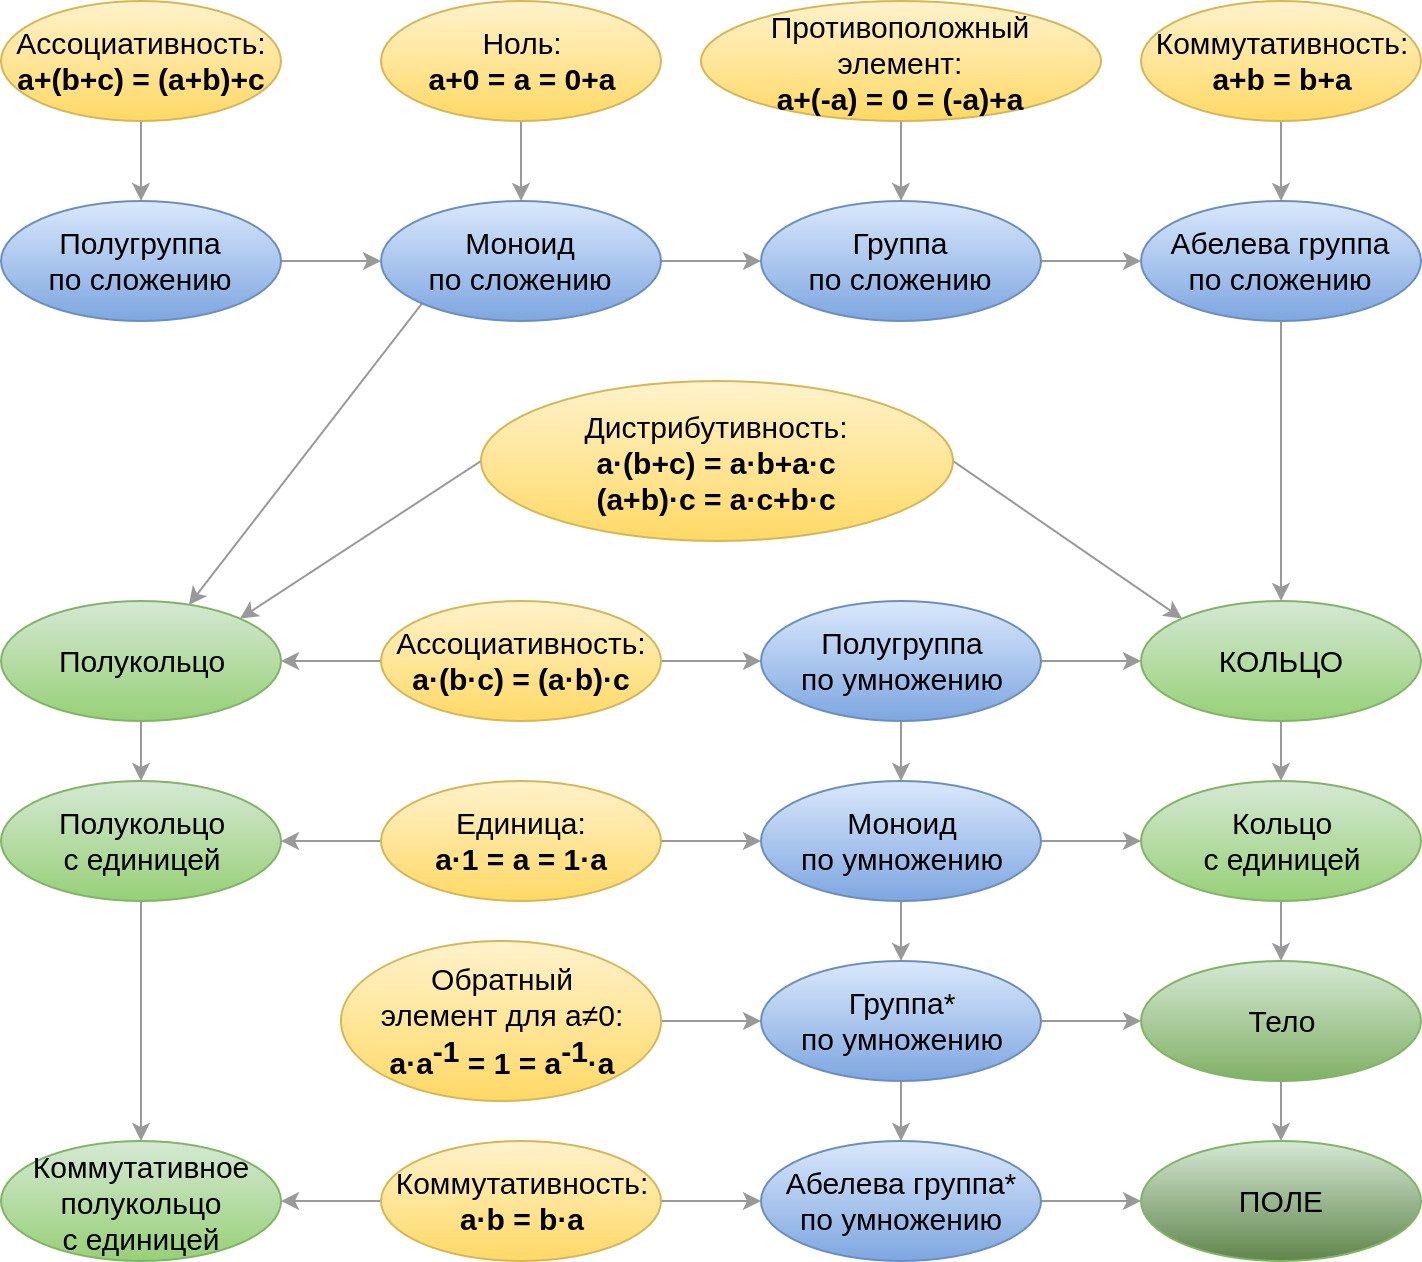
\includegraphics[scale=0.25]{Ring.png}
\end{center}
\caption{Звездочка означает, что исключены нулевые элементы.}\label{Ring}
\end{figure}

\item Заметка на будущее. Поле $\Q$ в общей алгебре определяется как минимальное поле, содержащее натуральные числа. Кроме того, поле рациональных чисел может быть задано как поле частных кольца $\Z$.

\end{enumerate}




\section{Соизмеримость. Иррациональности}

\lesson{Рциональные числа как расширение кольца целых чисел. Они определяются линейными уравнениями в целых числах. Разбор уравнения $x^2-2=0$. Доказательство иррациональности $\sqrt 2$ через ОТА, цепные дроби и графически. Несоизмеримость $\sqrt 2$ и 1. Рациональность $\Leftrightarrow$ конечная цепная дробь}

\begin{enumerate}
\item Рациональные числа мы определили как \textit{наклоны прямых}, заданных уравнениями вида $ax-by=0$, где $a$ и $b$ --- произвольные целые числа, причем $b\ne 0$. Оказалось, что наклон прямой с таким уравнением однозначно определяется пропорцией коэффициентов данного уравнения, т.е. рациональным числом $a/b$. Мы используем термин <<пропорция>> намеренно, чтобы подчеркнуть, что и наклон, и соответствующее ему рациональное число не меняются, если числитель и знаменатель дроби $a/b$ умножить на одно и то же целое число или разделить на общий делитель $a$ и $b$.

\item Говоря алгебраическим языком, рациональные числа --- это корни линейных уравнений, т.е. уравнений вида $a-by=0$, с целыми коэффициентами $a,b$.
\item Таким образом, выход в поле рациональных чисел происходит при попытке разрешить линейное уравнение, заданное над кольцом целых чисел.
\item Что, если мы рассмотрим линейное уравнение, но над полем рациональных чисел? Будет ли оно разрешимо?
\item Пусть $rx-q=0$ и $r,q\in\Q$. Тогда представим эти рациональные числа в виде дробей $r=a/b$, $q=c/d$, откуда
$$
0=rx-q = \frac{a}{b}x-\frac{c}{d} = \frac{adx-cb}{bd},
$$
откуда ясно, что данное уравнение эквивалентно линейному уравнению $(ad)x-(cb)=0$ с целыми коэффициентами, а значит, разрешимо в поле рациональных чисел.
\item Таким образом, поле $\Q$ замкнуто относительно взятия решений линейных уравнений. Термин <<замкнутость>>, или \textit{алгебраическая замкнутость} некоторой системы чисел, означает, что в этой системе можно найти корень алгебраического уравнения. При этом, в общем случае, алгебраическое уравнение --- это приравненное к нулю выражение, построенное из чисел данной числовой системы, некоторого набора переменных и разрешенных в в этой системе чисел алгебраических операций (сложения и умножения). В случае одной переменной такое уравнение имеет вид
$$
a_0 + a_1x + a_2x^2 + \dots + a_nx^n = 0.
$$
Позже мы еще вернемся к изучению таких уравнений произвольной степени $n$. А пока заметим, что линейное уравнение --- это алгебраическое уравнение при $n=1$. И поле $\Q$ разрешает любое такое уравнение.

\item Посмотрим, как оно справится с уравнениями более высокой степени! Рассмотрим уравнение $x^2-2=0$. Это --- уравнение второй степени с целыми коэффициентами (1 и 2), т.е. алгебраическое уравнение, заданное над $\Z$ (и над $\Q$). Разрешимо ли оно в $\Z$ или хотя бы в $\Q$?
\item Ответ: нет! Предположим, что $x=n/m$ разрешает такое уравнение, т.е. $(n/m)^2=2$. Предположим сразу же, что $n\perp m$, т.е. дробь $n/m$ несократимая. Далее имеем
$$
n^2=2m^2.
$$
Отсюда видно, что $n^2$ делится на 2, а значит, $2$ входит в разложение числа $n^2$ по степеням простых. Проблема в том, что если бы 2 не входила в разложение числа $n$, то ее не было бы и в разложении числа $n^2$, т.к. $n^2$ есть произведение степеней тех же самых простых, что и $n$, только в удвоенной степени. А значит, $n$ делится на 2, откуда следует, что $n^2$ делится на 4. Но тогда $m^2$ делится на 2 и, аналогично рассуждая, получаем, что и $m$ делится на 2. А это уже противоречит тому, что дробь $n/m$ несократимая --- ее как минимум можно сократить на 2.

Следовательно, корень уравнения $x^2-2=0$ не может быть рационалным числом.

\item Тем не менее, положительный корень такого уравнения можно оценивать сверху и снизу сколь угодно точно. Например, корень извлекается из числа 2.25 и равен 1.5, при этом $x^2=2<2.25$, так что $x<1.5$. В то же время, $2>1.96=1.4^2$, так что $x>1.4$. Можно еще усилить оценку: $1.41<x<1.42$. И так далее. Это позволяет нам думать, что на самом деле число такое есть, просто оно сидит где-то между рациональными числами. Обоснование его существования мы отложим на потом, а пока просто обозначим его $\sqrt 2$.
\item Есть еще один способ удостовериться в том, что $\sqrt 2$ не является рациональным числом. И тут снова нам на выручку приходят цепные дроби. Теперь-то мы вправе ими оперировать!

\item Воспроизведем алгоритм Евклида для дроби $\al = r_0/r_1$, считая, что $r_0>r_1$ (если это не так, то приведем дробь к виду $1/(r_1/r_0)$ и будем работать дальше только со знаменателем). Как и раньше, будем выделять остаток $r_{s+1}$ от деления $r_{s-1}$ на $r_s$ и сохранять неполное частное $k_s$. Только запишем весь алгоритм не в несколько строк, а в виде многоэтажной дроби. \index{Цепная дробь}
\begin{multline*}
\frac{r_0}{r_1} = \frac{k_1r_1+r_2}{r_1} = \boxed{k_1}+\frac{1}{\frac{r_1}{r_2}} =
\boxed{k_1} + \frac{1}{\frac{k_2r_2+r_3}{r_2}} =  \\
= \boxed{k_1} + \frac{1}{\boxed{k_2} + \frac{1}{r_3/r_2}} = 
\boxed{k_1} + \frac{1}{\boxed{k_2} + \frac{1}{\boxed{k_3} + \ddots \frac{1}{\boxed{k_n}+r_{n+1}/r_n}}},
\end{multline*}
где $r_0>r_1>r_2>\dots>r_n>r_{n-1}$.

\item Поскольку остатки всегда являются натуральными числами, рано или поздно этот алгоритм прервется. Пусть это случится на шаге с номером $n$, так что мы полагаем $r_{n+1}=0$, и цепная дробь закончится на числе $k_n$.
\item В таком случае цепную дорбь принято записывать последовательностью выделенных на каждом шаге целых частей:
$$
\frac{r_0}{r_1} = [k_1,k_2,\dots,k_n].
$$
\item Отсюда следует, что всякая рациональная дробь представима в виде конечной цепной дроби. Обратное, очевидно, также верно, ибо каждую конечную цепную дробь можно свернуть по правилам арифметики в обычную рациональную дробь.
\item Заметим также, что любое целое число представлятся в виде тривиальной цепной дроби, в которой есть только $k_1$.
\item Алгоритм Евклида можно применять к любым числам, лишь бы можно было выделять остаток от деления. Например, его можно применить к паре чисел $\pi/2$ и $\pi/3$ и получить конечную цепную дробь. А все потому, что отношение этих чисел является рациональным числом $3/2$. Поэтому, если отношение двух чисел $a/b$ рационально, их принято называть \textbf{соизмеримыми}.\index{Числа!соизмеримые}
\item\label{soizm} Соизмеримые числа хорошо иллюстрируются следующей картинкой: см. рис. \ref{soizmer2}.
\begin{figure}[hbt!]
\begin{center}
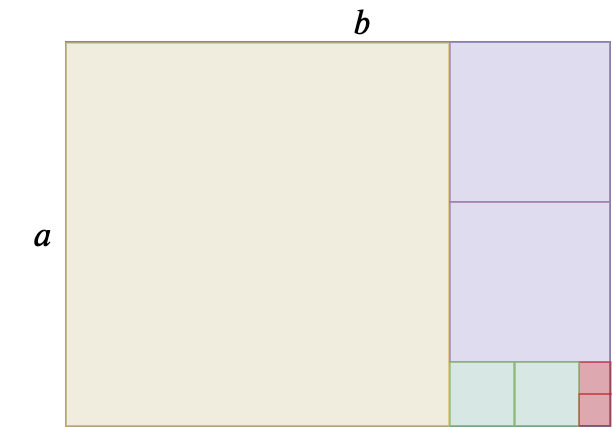
\includegraphics[scale=0.3]{soizmer.png}
\end{center}
\caption{}\label{soizmer2}
\end{figure}
Видим, что прямоугольник $a\times b$ мы делим на квадраты, каждый раз выбирая максимальный квадрат, который вписывается в оставшуюся область. Если $a$ и $b$ соизмеримы, то процесс разрезания прямоугольника на квадраты закончится за конечное число шагов, причем количества одинаковых квадратов, посчитанное в порядке их убывания, есть как раз те самые числа $k_1,k_2,\dots,k_n$, появляющиеся в записи цепной дроби (поскольку вырезание макисмального квадрата --- это не что иное как процесс выделения единица за единицей целой части из остатка, т.е. алгоритм Евклида).
\item То, что сами числа $a$ и $b$ при этом могут не быть целыми или рациональными --- не важно. Важно, что их отношение рационально. Также легко видеть, что всякое рациональное число соизмеримо с 1 и, наоборот, всякое число, соизмеримое с 1, рационально.
\item Посмотрим теперь, что происходит при попытке записать цепную дробь для $\sqrt 2$.
\item Мы уже знаем, что $1<\sqrt 2<2$, кроме того, $(\sqrt 2+1)=1/(\sqrt 2-1)$ (здесь работает формула $(x-y)(x+y)=x^2-y^2$, которую мы получили в разделе \ref{vizual} с помощью рис. \ref{razn}) так что
\begin{multline*}
\sqrt 2 = \boxed{1} + (\sqrt 2-1) = \boxed{1} + \frac{1}{1/(\sqrt 2-1)} = 
\boxed{1} + \frac{1}{\sqrt 2+1} = \\ 
= \boxed{1} + \frac{1}{\boxed{2} + (\sqrt 2-1)} = 
\boxed{1} + \frac{1}{\boxed{2} + \frac{1}{\sqrt 2+1}} = 
\boxed{1} + \frac{1}{\boxed{2} + \frac{1}{\boxed{2} + \frac{1}{\boxed{2} + \dots}}}
\end{multline*}
\item Как мы видим, остатком после выделения целой части всегда является одно и то же число $\sqrt 2-1$, и процесс алгоритма Евклида никогда не остановится. При этом цепная дробь характеризуется последовательностью одинаковых целых частей, равных 2. То есть представление для корня из 2 в виде цепной дроби будет бесконечным:
$$
\sqrt 2 = [1,2,2,2,2,2,\dots],
$$
и, следовательно, $\sqrt 2$ не является рациональным числом.
\item Геометричексий алгоритм Евклида здесь тоже зацикливается. Действительно, возьмем прямоугольник со сторонами $1+\sqrt 2$ и 1. Следуя алгоритму, вырежем из него два квадрата $1\times 1$. Посмотрим, какой прямоугольник остался: его сторонами будут $1$ и $\sqrt 2-1$. А в каком соотношении друг к другу они находятся?
$$
\frac{1}{\sqrt 2-1}=\frac{\sqrt{2}+1}{(\sqrt 2-1)(\sqrt 2+1)}=\sqrt 2+1.
$$
Таким образом, перед нами уменьшенная копия исходного прямоугольника. И если мы продолжим вырезать квдараты, мы будем вновь и вновь получать один и тот же прямоугольник, только всё меньшего размера.




\lesson{Иррациональное число. Поле $\Q[\sqrt 2]$. Дальнейшие расширения? Есть ли поле, не допускающее расширения?}

\item Числа, не яляющиеся рациональными, называются \textbf{иррациональными}.\index{Числа!иррациональные}
\item Наличие иррационального числа $\sqrt 2$ позволяет нам рассмотреть числа вида $r+q\sqrt 2$, где $r,q\in\Q$.
\item Множество таких чисел, полученных <<присоединением>> к полю $\Q$ положительного корня уравнения $x^2=2$ и любых таких выражений вида $r+q\sqrt 2$ с рациональными $r$ и $q$, принято обозначать $\Q[\sqrt 2]$ и называть \textbf{расширением поля} $\Q$.\index{Расширение поля}
\item Очевидно, что множество $\Q[\sqrt 2]$ замкнуто относительно сложения, т.к.
$$
(r_1+q_1\sqrt 2)+(r_2+q_2\sqrt 2)=(r_1+r_2)+(q_1+q_2)\sqrt 2,
$$
т.е. является числом такого же вида. Аналогично можно увидеть, что и произведение таких чисел имеют тот же вид:
$$
(r_1+q_1\sqrt 2)(r_2+q_2\sqrt 2)=(r_1r_2+2q_1q_2)+(r_1q_2+r_2q_1)\sqrt 2,
$$
т.е. в обоих случаях результат снова находится в $\Q[\sqrt 2]$.
\item Таким образом, множество $\Q[\sqrt 2]$ замкнуто относительно операций сложения, вычитания, умножения и деления. Проверим, что для него выполняются все аксиомы поля F1--F8, приведенные на стр. \pageref{FildAxiom}.

F1: замкнутость операций мы только что проверили.

F2: ассоциативность операций
\begin{multline*}
(r_1+q_1\sqrt 2 + r_2+q_2\sqrt 2)+(r_3+q_3\sqrt 2) = (r_1+r_2+r_3)+(q_1+q_2+q_3)\sqrt 2 = \\
=(r_1+q_1\sqrt 2) + (r_2+q_2\sqrt 2+r_3+q_3\sqrt 2),
\end{multline*}
\begin{multline*}
[(r_1+q_1\sqrt 2)(r_2+q_2\sqrt 2)](r_3+q_3\sqrt 2) = \\
=(r_1r_2r_3 + 2q_1q_2r_3 + 2r_1q_2q_3 + 2q_1r_2q_3) + (r_1r_2q_3 + 2q_1q_2q_3 + r_1q_2r_3 + q_1r_2r_3)\sqrt 2 = \\
=(r_1+q_1\sqrt 2)[(r_2+q_2\sqrt 2)(r_3+q_3\sqrt 2)].
\end{multline*}

F3: коммутативность операций
\begin{multline*}
(r_1+q_1\sqrt 2)+(r_2+q_2\sqrt 2) = (r_1+r_2)+(q_1+q_2)\sqrt 2 = \\
= (r_2+r_1)+(q_2+q_1)\sqrt 2 = (r_2+q_2\sqrt 2)+(r_1+q_1\sqrt 2),
\end{multline*}
\begin{multline*}
(r_1+q_1\sqrt 2)(r_2+q_2\sqrt 2) = (r_1r_2+2q_1q_2)+(r_1q_2+r_2q_1)\sqrt 2 = \\
=(r_2r_1+2q_2q_1)+(r_2q_1+r_1q_2)\sqrt 2 = (r_2+q_2\sqrt 2)(r_1+q_1\sqrt 2).
\end{multline*}

F4: существование нуля $0+0\sqrt 2$.

F5: противоположный элемент $-r-q\sqrt 2$.

F6: существование единицы $1+0\sqrt 2$.

F7: существование обратного элемента
$$
\frac{1}{r+q\sqrt 2} = \frac{r-q\sqrt 2}{(r+q\sqrt 2)(r-q\sqrt 2)} = \frac{r-q\sqrt 2}{r^2-2q^2}.
$$
При этом нужно показать, что $r^2-2q^2\ne 0$, если $r$ и $q$ одновременно не обращаются в ноль. Предположим, что это не так, т.е. $r^2=2q^2$, причем $q\ne 0$ (ясно, что тогда и $r\ne 0$), тогда $2=(r/q)^2$, но тогда $\sqrt 2$ --- рациональное число. Противоречие. Следовательно, если $r+q\sqrt 2\ne 0$, то оно обратимо.

F8: дистрибутивность
\begin{multline*}
[(r_1+q_1\sqrt 2) + (r_2+q_2\sqrt 2)](r_3+q_3\sqrt 2) = \\
= (r_1r_3+r_2r_3+2q_1q_3+2q_2q_3) + (r_1q_3+r_2q_3+r_3q_1+r_3q_2)\sqrt 2 = \\
= (r_1+q_1\sqrt 2)(r_3+q_3\sqrt 2) + (r_2+q_2\sqrt 2)(r_3+q_3\sqrt 2).
\end{multline*}

\item Итак, множество $\Q[\sqrt 2]$ с обычными операциями сложения и умножения является полем.
\item В поле $\Q[\sqrt 2]$ уравнение $x^2-2=0$ разрешимо. Причем в нем лежат оба корня данного уравнения: $\sqrt 2$ и $-\sqrt 2$.
\item Отметим еще один важный факт. В поле $\Q[\sqrt 2]$ выражение $x^2-2$ можно записать в виде произведения линейных членов $(x-\sqrt 2)(x+\sqrt 2)$, поскольку $\sqrt 2$ здесь стал <<разрешенным>> числом. Точно так же мы ранее сначала не могли записывать уравнения $0.5x-1=0$, т.к. работали только с целыми числами (но могли заменить его эквивалентным уравнением $x-2=0$), а после выхода в поле $\Q$ у нас появилась возможность использовать дробные коэффициенты.
\item Возникает резонный вопрос: а если уравнение какое-то более сложное? Например, $x^5+3x^3-5=0$. Всегда ли его можно разложить на линейные множители в поле $\Q[\sqrt 2]$? Или понадобится какое-то новое расширение $\Q$?
Иначе говоря, всегда ли будут корни такого уравнения лежать в построенных нами полях?
\item Ответ: нет. Но существует такое всеобъемлющее поле, в котором это действительно возможно. И постепенно мы дойдем и до него...
\end{enumerate}


\subsection*{Задачи}

\begin{enumerate}
\item Разложите в цепную дробь числа $9/5$, $22/7$, $3/13$, $55/27$.
\item Какие число и цепная дробь зашифрованы на картинке \ref{soizmer2}?
\item Найти цепную дробь для $\sqrt 3$.
\item Найти цепную дробь для отношения 
$$
\frac{\sqrt 2+1}{\sqrt 2-1}.
$$
Соизмеримы ли эти числа?
\end{enumerate}




\begin{comment}
\chapter{8. Исчисление остатков}
\end{comment}
\newchapter{Исчисление остатков}\label{ostatki}

\vrezka{
Арифметика остатков дает богатый фактологичекий материал для изучения свойств простых чисел, а также позволяет по-новому взглянуть на операции Минковского с числовыи множествами и выйти на такие важные вехи теории множеств, как виды отношений и фактормножества.
}

\section{Арифметика остатков}

\lesson{Сюжет с минутами и часами. Исчисление дней недели. Високосные годы. Определение сравнения чисел по модулю.}

\begin{enumerate}
\item Рассмотрим бытовую задачу. Вам нужно выключить печку через 40 минут, но у вас нет таймера, зато есть будильник, на котором можно выставить время звонка. Сейчас 12:30, на какое время требуется поставить будильник? Ответ: 13:10. Почему так? Дело в том, что в часе 60 минут, и если к 30 минутам прибавить 40, то получается 70 минут, что больше часа. Поэотму добавляем 1 час и остаток --- 10 минут.
\item Еще пример: сколько часов будет через 20 часов, если сейчас 8 утра? Можно решать аналогично: $8+20=28$, затем убираем полные сутки, т.е. 24 часа, остается 4 часа утра.
\item Можно решать иначе. 20 часов --- это $-4$ часа от суток. Следовательно, нужно просто вычесть из 8 утра 4 часа и получим те же 4 часа утра.
\item Во всех случаях мы решаем задачу нахождения остатка от деления на некоторое число. В случае минут это 60, в случае часов это 24.
\item Когда вас просят отметить в анкете количество полных лет, то вам по сути нужно найти неполное частное от деления вашего возраста на 1 год. Конечно, в данном случае нам это просто сделать, т.к. каждый год мы запоминаем именно количество прожитых лет, а не дней или недель.
\item Но, например, во многих сферах деятельности планирование календаря происходит неделями (и даже у себя в компьютере в настройках календаря вы можете вывести номер текущей недели в году). А сколько недель в году? Для этого нужно найти неполное частное от деления 365 (или 366) на 7, оно составляет 52.
\item Остаток от деления на неделю есть число от 0 до 6, которое определяет сдвиг вперед относительно текущего дня недели. Например, если сегодня четверг, то какой день недели будет через 30 дней? Мы выбрасываем 4 полных недели, что составляет 28 дней, и находим остаток, который равен 2. Это значит, что через 30 дней будет четверг плюс 2 дня, т.е. суббота.
\item Точно так же можно легко заметить, что каждый год происходит смещение дат на один или два дня вперед относительно дней недели. Так, если в этом году 1 января было средой, то в следующем оно будет или четвергом (если мы не переходим через 29 февраля), или пятницей (если текущий год --- високосный, т.е. содержит 366 дней), как на картинке \ref{weekdays}.
\begin{figure}[hbt!]
\begin{center}
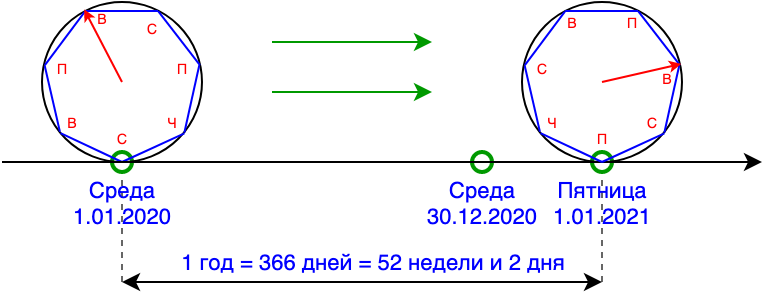
\includegraphics[scale=0.4]{weekdays.png}
\end{center}
\caption{}\label{weekdays}
\end{figure}
\item Каждые 28 лет (а 28 --- это наименьшее общее кратное 7 и 4) соответствие дат и дней недели повторяется.
\item Если выписать последовательно сдвиг дней недели год за годом, то легко увидеть, что 28-летный цикл разбивается на несколько подциклов, через которые даты тоже повторяются. Рис. \ref{timeshift} дает представление о том, как это происходит: сначала даты повторяются через 6 лет (если текущая дата находится в интервале от 1 марта високосного года до 28 февраля следующего года), затем --- через 11 лет, затем снова через 6 лет, затем --- через 5 лет.
\begin{figure}[hbt!]
\begin{center}
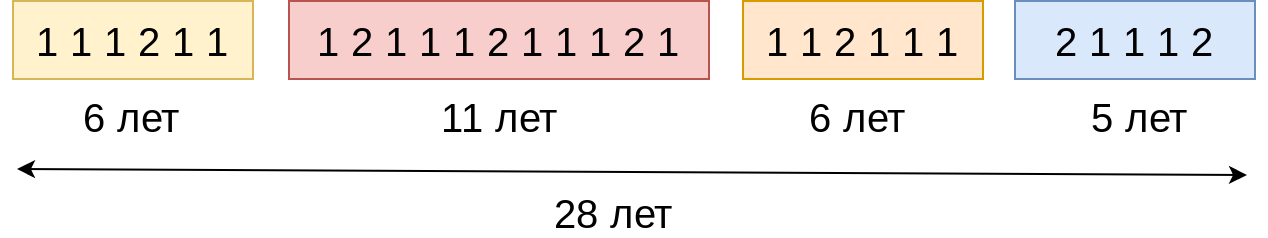
\includegraphics[scale=0.25]{timeshift.png}
\end{center}
\caption{}\label{timeshift}
\end{figure}

\item При расчетах на более длительные периоды, а именно, при переходе через 1900 год или 2100 год, нужно учитывать также, что 3 раза за 400 лет не происходит добавление лишнего дня (29 февраля) для более точного соответствия календаря астрономическому году, т.е. 1900, 1800, 1700 годы не являются високосными, как и 2100, 2200 и 2300.
\item Иными словами, часто в жизни встречается задача вычисления дня недели, и здесь нам на помощь приходит исчисление остатков по модулю 7. Например, сегодня 21 марта 2020 года, суббота, а нам нужно знать, какой день недели будет 31 августа 2020 года. Сначала мы находим день недели 21 августа, т.к. до этой даты целое число месяцев. При этом мы 3 раза переходим через 31 число (март, май, июль) и 2 раза --- не переходим (апрель, июнь). Следовательно, 3 раза прибавляется остаток 3, и 2 раза --- остаток 2, итого сумма остатков составляет 13. Но это больше 7, причем очень близко к 14, поэтому сумму остатков мы запишем как -1. Наконец, остается добавить 10 дней (от 21 августа до 31 августа). Итого получается 9, а по модулю 7 --- всего 2. Таким образом, 31 августа 2020 года есть понедельник!
\item Из приведенной выше картинки с семиугольником на окружности, совмещенной с прямой линией, мы можем ясно представить себе, как работает исчисление остатков по модулю 7, т.е. исчисление дней недели. Мы катим окружность по прямой времени, пока не достигнем нужной нам даты. При этом неважно, сколько целых оборотов совершит семиугольник, т.е. сколько недель мы проедем, а вот последний неполный виток как раз и дает нам ответ на вопрос о дне недели. Так что, если мы пронумеруем дни недели цифрами от 0 до 6, то любое расстояние между датами можно представить как какое-то целое количество недель плюс остаток, лежащие в диапазоне от 0 до 6 (включительно).
\item Эта картинка легко обобщается на случай произвольного основания. Представим, что в неделе у нас не 7 дней, а, например, 28 (лунный месяц), и тогда любое расстояние между датами выражается как целое число 28-дневных циклов плюс некоторый остаток от 0 до 27. И так далее.
\item Следующим шагом обобщения является выход в целые числа. Ведь рассчитывать день недели можно не только в будущее, но и в прошлое с соответствующей сменой знака перед величиной сдвига. Так, если сегодня воскресенье, то 10 дней назад (-10) день недели был на 3 дня меньше (-3) или же на 4 дня больше, т.е. четверг.
\item Таким образом мы приходим к тому, что всякое целое число $a$ можно представить в виде $a=km+r$, где $k$ --- неполное частное от деления $a$ на положительное $m$, $r$ --- остаток от деления, который находится в промежутке от 0 (включая) до $m$ (не включая). Если число $b$ имеет такой же точно остаток от деления на $m$, т.е. имеет место равенство $b=lm+r$ при не котором целом $l$, то говорят, что числа \textbf{$a$ и $b$ сравнимы по модулю $m$}. Это записывается следующим образом:
$$
a\equiv b\pmod m.
$$
Читается: $a$ \textbf{сравнимо с} $b$ (по модулю $m$).\index{Отношение!сравнимости по модулю}\index{Сравнение по модулю}

Причем, если модуль $m$ известен из контекста и не меняется при вычислениях, то его можно опускать, записывая просто $a\equiv b$. 

\item На картинке, приведенной выше, даты 01.01.2020 и 30.12.2020 сравнимы по модулю 7, т.е. по дням недели, что и суммируется фразой <<это --- один и тот же день недели>>.
А про интервал в 366 дней мы запишем $366\equiv 2\pmod 7$. Такая запись никак не информирует нас о коэффициенте $k$ (количестве целых недель), но показывает самое главное --- сколько дней надо прибавить к среде.


\lesson{Таблицы сложения и умножения по данному модулю. Анализ строк таблицы умножения с нулями и теорема об остатках. Сравниваем $\Z_5^*$ и $\Z_8^*$}

\item Остатками можно оперировать так же, как обычными числами, сбрасывая всякий раз накопленные при сложении целые <<обороты>> модулей. Иначе говоря, если мы хотим, например, к текущей среде прибавить 6 дней, то мы совмещаем наш семиугольник вершиной <<среда>> с прямой времени, а затем прокатываем его вперед на 6 делений (что чуть меньше полного оборота), и в точке касания с прямой получаем вторник. Заметим, что ровно тот же результат мы получим, если прокатим семиугольник назад на 1 деление. Это значит, что числа 6 и -1 сравнимы по модулю 7. И на практике можно также пользоваться отрицательными числами для исчисления остатков.
\item Ранее мы много времени уделяли таблицам композиций движений многоугольников. И, как мы помним, композиция вращений многоугольника соответствовала сложению углов этих вращений. При этом мы также отбрасывали 360 градусов (или $2\pi$), если сумма углов переваливала за полный оборот. При описании конечных подгрупп движений правильных многоугольников мы выяснили, что каждый поворот является степенью некоторого минимального поворота на угол $2\pi/n$ (для $n$-угольника), т.е. все повороты выражаются углами $k(2\pi/n)$, где $k=0,\dots,n-1$ (ничего не напоминает?).
\item Понаблюдаем теперь за степенями этих поворотов при композициях, т.е. при сложении углов. Для примера рассмотрим случаи $n=7$ и $n=8$, и выпишем таблицу композиций, которая представлят собой таблицу сложения остатков по модулям 7 и 8, соответственно.
\item Таблицы сложения остатков по модулям 7 и 8:\index{Таблица сложения по модулю}
\begin{center}
\begin{tabular}{c||c|c|c|c|c|c|c|}
  & 0 & 1 & 2 & 3 & 4 & 5 & 6 \\ \hline\hline
0 & 0 & 1 & 2 & 3 & 4 & 5 & 6 \\ \hline
1 & 1 & 2 & 3 & 4 & 5 & 6 & 0 \\ \hline
2 & 2 & 3 & 4 & 5 & 6 & 0 & 1 \\ \hline
3 & 3 & 4 & 5 & 6 & 0 & 1 & 2 \\ \hline
4 & 4 & 5 & 6 & 0 & 1 & 2 & 3 \\ \hline
5 & 5 & 6 & 0 & 1 & 2 & 3 & 4 \\ \hline
6 & 6 & 0 & 1 & 2 & 3 & 4 & 5 \\ \hline
\end{tabular}
\quad
\begin{tabular}{c||c|c|c|c|c|c|c|c|}
  & 0 & 1 & 2 & 3 & 4 & 5 & 6 & 7 \\ \hline\hline
0 & 0 & 1 & 2 & 3 & 4 & 5 & 6 & 7 \\ \hline
1 & 1 & 2 & 3 & 4 & 5 & 6 & 7 & 0 \\ \hline
2 & 2 & 3 & 4 & 5 & 6 & 7 & 0 & 1 \\ \hline
3 & 3 & 4 & 5 & 6 & 7 & 0 & 1 & 2 \\ \hline
4 & 4 & 5 & 6 & 7 & 0 & 1 & 2 & 3 \\ \hline
5 & 5 & 6 & 7 & 0 & 1 & 2 & 3 & 4 \\ \hline
6 & 6 & 7 & 0 & 1 & 2 & 3 & 4 & 5 \\ \hline
7 & 7 & 0 & 1 & 2 & 3 & 4 & 5 & 6 \\ \hline
\end{tabular}
\end{center}
Таблица сложения получается последовательными циклическими сдвигами верхней строки влево.

\item Нетрудно видеть, что сложение по модулю удовлетворяет аксиомам абелевой группы, т.е. сложение ассоциативно, коммутативно, существует ноль, и для всякого элемента существует противоположный. Эти свойства наследуются из кольца $\Z$.

\item Помимо сложения остатков мы можем их умножать (в терминологии вращений многоугольника умножение соответствует многократной композиции одинаковых поворотов, так что первое число произведения отвечает за величину поворота, а второе --- за его кратность, либо наоборот). Таблицы умножения остатков по модулям 7 и 8 (отметим важную особенность этих таблиц: они имеют центральную симметрию, если вычеркнуть нулевые строку и столбец) выглядят так:\index{Таблица умножения по модулю}
\begin{center}
\begin{tabular}{c||c||c|c|c|c|c|c|}
  & 0 & 1 & 2 & 3 & 4 & 5 & 6 \\ \hline\hline
0 & 0 & 0 & 0 & 0 & 0 & 0 & 0 \\ \hline\hline
1 & 0 & 1 & 2 & 3 & 4 & 5 & 6 \\ \hline
2 & 0 & 2 & 4 & 6 & 1 & 3 & 5 \\ \hline
3 & 0 & 3 & 6 & 2 & 5 & 1 & 4 \\ \hline
4 & 0 & 4 & 1 & 5 & 2 & 6 & 3 \\ \hline
5 & 0 & 5 & 3 & 1 & 6 & 4 & 2 \\ \hline
6 & 0 & 6 & 5 & 4 & 3 & 2 & 1 \\ \hline
\end{tabular}
\qquad
\begin{tabular}{c||c||c|c|c|c|c|c|c|}
  & 0 & 1 & 2 & 3 & 4 & 5 & 6 & 7 \\ \hline\hline
0 & 0 & 0 & 0 & 0 & 0 & 0 & 0 & 0 \\ \hline\hline
1 & 0 & 1 & 2 & 3 & 4 & 5 & 6 & 7 \\ \hline
2 & 0 & 2 & 4 & 6 & 0 & 2 & 4 & 6 \\ \hline
3 & 0 & 3 & 6 & 1 & 4 & 7 & 2 & 5 \\ \hline
4 & 0 & 4 & 0 & 4 & 0 & 4 & 0 & 4 \\ \hline
5 & 0 & 5 & 2 & 7 & 4 & 1 & 6 & 3 \\ \hline
6 & 0 & 6 & 4 & 2 & 0 & 6 & 4 & 2 \\ \hline
7 & 0 & 7 & 6 & 5 & 4 & 3 & 2 & 1 \\ \hline
\end{tabular}
\end{center}

Заметим, что умножение по модулю удовлетворяет аксиомам абелева моноида, т.е. оно ассоциативно, коммутативно и имеет нейтральный элемент --- единицу. Эти свойства умножения наследуются из кольца $\Z$.

\item Таким образом, множество $\{0,1,2,\dots,m-1\}$ с операциями сложения и умножения по модулю $m$ является конечным коммутативным кольцом с единицей. Оно называется \textbf{кольцом вычетов по модулю} $m$ и обозначается так: $\Z_m$.\index{Группа!вычетов}\index{Кольцо!вычетов}

\item Отметим еще одно свойство умножения: строка или столбец, номер которого НЕ взаимно прост с модулем, содержит нули. Это легко доказать. Пусть номер строки равен $k$, и $s=\gcd(k,m)>1$. При этом ясно, что $s<m$, т.к. $s$ является делителем $m$. Пусть также $t=m/s$. Рассмотрим тогда строку $k$ и столбец $t$. Произведение их номеров равно $kt=km/s$. Поскольку $k/s$ также целое, получаем, что $kt$ кратно $m$, а значит, $kt\equiv 0\pmod m$. Отметим, что $s=1$ здесь не проходит ровно потому, что в этом случае $t$ не будет номером столбца таблицы умножения.
\item На самом деле верно и обратное: если строка таблицы умножения содержит нули, то номер строки не взаимно прост с модулем. Для этого мы докажем эквивалентное утверждение
\begin{thrm}\label{k2k3k}
Пусть $k>0$  и  $k\perp m$, тогда все остатки
$$
k,\quad 2k,\quad 3k,\quad\dots,\quad (m-1)k\pmod m
$$
попарно различны и отличны от нуля.
\end{thrm}
\pf Предположим, что один из остатков равен нулю: $kl\equiv 0\pmod m$, где $l\in\{1,2,\dots,m-1\}$. Тогда $kl=mt$ при некотором $t$. Но поскольку $k\perp m$, в силу ОТА число $k$ делит $t$, а значит, $k\le t$. Однако $l<m$, следовательно, $kl<mt$. Противоречие.

Далее, если среди остатков есть равные, например, $kl\equiv kt$, то найдется и остаток $k(l-t)$ (или $k(t-l)$, если $t>l$), который равен 0. А это невозможно по доказанному. 

Таким образом, эти остатки все различны и положительны, а значит, являются перестановкой множества $\{1,2,\dots,m-1\}$.
\epf

\item Появление нулей в таблице умножения по непростому модулю означает, что в кольце вычетов по непростому модулю существуют \textit{делители нуля}, т.е. такие ненулевые элементы, произведение которых равно нулю. Это --- существенное отличие числовой системы $\Z_m$ от тех, что мы встречали ранее.

\item Множество $\Z_m^*$, состоящее только из взаимно простых с модулем $m$ элементов $\Z_m$, образует абелеву группу по умножению по модулю $m$. Действительно, умножение замкнуто на множестве $\Z_m^*$, т.е. если $k\perp m$ и $l\perp m$, то $kl\perp m$ (это следует из основной теоремы арифметики: просто делитель $m$ и $kl$ будет и простым делителем одного из чисел $k$ или $l$).

Коммутативность умножения остатков наследуется от умножения в кольце целых чисел.

1 является элементом $\Z_m^*$.

Чтобы доказать, что у произвольного элемента $k\in\Z_m^*$ имеется обратный, вспомним алгоритм Евклида, а точнее, его следствие: поскольку $k\perp m$, существуют такие целые числа $a$ и $b$, что $ka+mb=1$. Тогда число $ka+mb\equiv 1\mod m$, а значит, $ka\equiv 1\mod m$. Наконец, если $a=lm+r$, то верно равенство $kr\equiv 1\mod m$, т.е. остаток $r$ является обратным к остатку $k$ при умножении по модулю.

Остается показать, что $r\in \Z_m^*$, т.е. что $r\perp m$. Пусть $q|r$ и $q|m$. Тогда $q|a$ и, следовательно, $q|(ka+mb)$, т.е. $q|1$, откуда следует, что $q=\pm 1$. А это и означает, что $r$ и $m$ взаимно просты, т.е. $r\in\Z_m^*$. Тем самым, обратный элемент для произвольного остатка $k\in\Z_m^*$ существует и принадлежит $\Z_m^*$.

Следовательно, $\Z_m^*$ --- группа по умножению по модулю $m$.

\item Пусть $p$ --- простое число. В этом случае все числа $1,2,\dots,p-1$ взаимно просты с $p$, так что $\Z_p^*=\{1,2,\dots,p-1\}$. И поскольку, как мы только что выяснили, $\Z_p^*$ является абелевой группой по умножению по модулю $p$, получаем, что $\Z_p$ с операциями сложения и умножения по модулю $p$ удовлетворяет аксиомам поля.

\item $\Z_p$ при простом $p$ --- это наш первый пример \textit{конечного поля}!

\item Рассмотрим таблицы умножения для групп $\Z_5^*$ и $\Z_8^*$:
\begin{center}
\begin{tabular}{c||c|c|c|c|}
$\Z_5^*$  & 1 & 2 & 3 & 4 \\ \hline\hline
        1 & 1 & 2 & 3 & 4 \\ \hline
        2 & 2 & 4 & 1 & 3 \\ \hline
        3 & 3 & 1 & 4 & 2 \\ \hline
        4 & 4 & 3 & 2 & 1 \\ \hline
\end{tabular}
\qquad
\begin{tabular}{c||c|c|c|c|}
$\Z_8^*$  & 1 & 3 & 5 & 7 \\ \hline\hline
        1 & 1 & 3 & 5 & 7 \\ \hline
        3 & 3 & 1 & 7 & 5 \\ \hline
        5 & 5 & 7 & 1 & 3 \\ \hline
        7 & 7 & 5 & 3 & 1 \\ \hline
\end{tabular}
\end{center}
\item И тут мы снова видим знакомую ситуацию: если группа $\Z_5^*$ циклическая (все ее элементы могут быть получены как степени двойки), и ее можно изоморфно сопоставить с группой $\Z_4$ с операцией сложения, а также с группой вращений квадрата, то группа $\Z_8^*$ уже не является циклической, хотя остается абелевой. И это --- еще одна ипостась четверной группы Клейна. Чуть позже мы дадим сравнение нескольких ипостасей групп 4-го порядка.

\end{enumerate}



\subsection*{Задачи}
\begin{enumerate}
\item Если сегодня понедельник, то какой день недели будет через 10 дней, через 90 дней, через 2 года (невисокосных)?
\item Найти день недели через месяц, квартал, полгода и год, отправляясь от текущей даты.
\item Построить таблицы сложения и умножения для модулей: 2,3,4,5,6.
\item Сравнить таблицу сложения остатков по модулю 2 с таблицами умножения классов сдвигов $\T$ и симметрий $\S$ для прямой и окружности.
\item Сравнить таблицу симметрий ромба с таблицей умножения группы $\Z_8^*$.
\item В группе $\Z_8^*$ найти обратные элементы: $3^{-1}, 5^{-1}, 7^{-1}$.
\item Проверить, что $\Z_m$ удовлетворяет аксиомам кольца.
\end{enumerate}

\section{Свойства арифметики остатков}


\lesson{Вывод основных арифметических свойств сравнений, китайская теорема об остатках}

\begin{enumerate}
\item Свойства сравнений таковы (предлагается в качестве упражнения):
\begin{enumerate}[M1.]
\item $a\equiv b\pmod m$ тогда и только тогда, когда $a-b$ кратно $m$;
\item если $a\equiv b$, $c\equiv d$, то $a+c\equiv b+d$, $a-c\equiv b-d$ и $ac\equiv bd$;
\item для $n\ge 0$ если $a\equiv b$, то $a^n\equiv b^n$;
\item признаки делимости на $3$ и на $9$: $a_0+a_110+a_210^2+\dots+a_n10^n\equiv a_0+\dots+a_n$ по модулю $3$ и по модулю $9$;
\item если $m>0$ и $d\perp m$, то
$$
ad\equiv bd\pmod m\iif a\equiv b\pmod m
$$
\item  если $m,d>0$, то
$$
ad\equiv bd\pmod{md}\iif a\equiv b\pmod m
$$
\item  если $m>0$, то для любого $d$
$$
ad\equiv bd\pmod m\iif a\equiv b\pmod{m/\gcd(m,d)}
$$
\item  если $m,d>0$, $a\equiv b\pmod{md}$, то $a\equiv b\pmod{m}$
\item если $m,n>0$, то
$$
a\equiv b\pmod m,\quad a\equiv b\pmod n\iif a\equiv b\pmod{\nok(m,n)}
$$
\item если $m,n>0$ и $m\perp n$, то
$$
a\equiv b\pmod m,\quad a\equiv b\pmod n\iif a\equiv b\pmod{mn}
$$
\item пусть $n_p$ --- степень простого числа $p$ в разложении $n$ по степеням простых (ОТА), тогда
$$
a\equiv b\pmod n\iif \forall p\quad a\equiv b\pmod{p^{n_p}}\quad\textup{($p$ --- простое)}
$$
\end{enumerate}
\item Что если у нас задана система из нескольких сравнений, и требуется знать, разрешима ли она? Ответ на этот вопрос дает
\begin{thrm}[Китайская теорема об остатках]
Если натуральные числа $m_{1},m_{2},\dots, m_{n}>0$ попарно взаимно просты, то для любых целых
$r_{1},r_{2},\dots ,r_{n}$ таких, что $0\leqslant r_{i}<m_{i}$ при всех $i\in \{1,2,\dots ,n\}$, найдётся число $N$, которое при делении на $m_{i}$ даёт остаток $r_{i}$ при всех $i\in \{1,2,\dots ,n\}$.

Более того, если найдутся два таких числа $N_1$ и $N_2$, то $N_{1}\equiv N_{2}\pmod  {m_{1}\cdot m_{2}\cdot \ldots \cdot m_{n}}$.
\end{thrm}
\pf
Рассмотрим систему уравнений:
\begin{equation}\label{sischine}
\begin{cases}
x\equiv r_{1}{\pmod {m_{1}}},\\
x\equiv r_{2}{\pmod {m_{2}}},\\
\cdots \cdots \cdots \cdots \cdots \cdots \\
x\equiv r_{n}{\pmod {m_{n}}}.
\end{cases}
\end{equation}

Покажем, что если наборы $(r_{1},r_{2},\dots ,r_{n})$ и $(m_{1},m_{2},\dots ,m_{n})$ удовлетворяют условию теоремы, то решение системы \eqref{sischine} существует и единственно с точностью до операции взятия по модулю $m$, где $m=m_1m_2\dots m_n$, причем справедлива формула:
\begin{equation}\label{decitionchine}
x=\sum _{{j=1}}^{n}r_{j}M_{j}M_{j}^{{-1}},
\end{equation}
где $M_{j}=\frac m{m_{j}}$, а $M_{j}^{{-1}}$ --- мультипликативно обратный к $M_{j}$ группе $\Z_{m_j}^*$. Отметим, что обратный $M_j^{-1}$ существует, т.к. $M_j\not\equiv 0\mod m_j$ в силу условий теоремы.

Покажем, что определённый таким образом $x$ является решением --- проверим, что для него выполняется $i$-е равенство в системе \eqref{sischine}.

Если $j\ne i$, то $j$-е слагаемое в \eqref{decitionchine} сравнимо с нулем по модулю $m_i$, поскольку $M_j$ кратно $m_i$, поэтому сумма \eqref{decitionchine} превращается лишь в одно слагаемое при $j=i$ (по модулю $m_i$):
$$
x\equiv r_{i}M_{i}M_{i}^{{-1}}\equiv r_i\pmod m_i,
$$
последнее сравнение верно, т.к. $M_i^{-1}$ является обратным к $M_i$ именно по модулю $m_i$. Следовательно,
$x$ является решением системы \eqref{sischine}.

Число $x$ нами вычислено в обычной арифметике целых чисел. Покажем, что его выбор можно осуществлять с точностью до вычисления остатка по модулю $m$. Пусть $y\equiv x\mod m$. Тогда $y=mk+x$ при некотором целом $k$. Так как $m$ делится на $m_i$ при всех $i=\overline{1,n}$, то $y\equiv x\mod m_i$, т.е. также является решением системы \eqref{sischine}.

Осталось показать, что если $y\not\equiv x\mod m$, то $y$ не является решением данной системы (единственность решения по модулю). Действительно, если $y$ и $x$ одновременно являются решениями системы \eqref{sischine}, то $y-x \equiv r_i\mod m_i$ при всех $i\overline{1,n}$, т.е. $y-x$ делится на все $m_i$, а значит, делится и на их произведение (т.к. все они попарно взаимно просты). Тогда $y-x=mk$ при не котором целом $k$, т.е. $y\equiv x\mod m$.

Итак, решениями системы \eqref{sischine} являются те и только те целые числа, которые сравнимы с $x$, заданным формулой \eqref{decitionchine}, по модулю $m=m_1m_2\dots m_n$.
\epf



\lesson{Малая теорема Ферма. Простое доказательство путем перемножения всех остатков, а также графическое доказательство с циклами}

\begin{thrm}[Малая теорема Ферма]
$n^{p-1}\equiv 1\pmod p$, где $p$ --- простое, и $n\not\vdots p$.\index{Теорема!малая теорема Ферма}
\end{thrm}

Согласно теореме \ref{k2k3k} все остатки
$$
n,2n,3n,\dots,(p-1)n\pmod p
$$
различны и составляют множество $\{1,2,\dots,p-1\}$. Тогда по свойствам сравнений будем иметь
$$
n\cdot 2n\cdot 3n \dots(p-1)n\equiv 1\cdot 2\cdot 3\dots (p-1)\pmod p,
$$
откуда $n^{p-1}(p-1)!\equiv (p-1)!\pmod p$. Последнее тождество можно сократить на $(p-1)!$, поскольку все его множители взаимно просты с $p$. Откуда получаем
$$
n^{p-1}\equiv 1\pmod p.
$$

\item Малая теорема Ферма позволяет вычислять обратный элемент по умножению в поле $\Z_p$. Достаточно $n$ умножить на $n^{p-2}$, и мы получим 1. Но такой способ нахождения обратного элемента довольно трудоемкий. Проще всего воспользоваться алгоритмом Евклида, а точнее, его представлением в виде цепной дроби.

Пусть, например, $p=101$. Это --- простое число. И пусть требуется найти $77^{-1}$ по модулю $101$. Можно восопльзоваться малой теоремой Ферма и вычислить $77^{99}\mod 101$. Число
\begin{align*}
77^{99} =\; & 578870998719483192604006423068948796479127581676622586145657719 \\
            & 488743965292466241833275096332117841891352380031908081644221279 \\
            & 6787687881706201273681438984199647603820668204476189223565013,
\end{align*}
как и его остаток от деления на 101, без компьютера не вычислить.

Теперь выпишем цепную дробь:
$$
\frac{101}{77} = 1 + \frac{1}{3 + \frac{1}{5 - \frac 15}},
$$
откуда, отсекая <<хвост>> $1/5$, сворачиваем дробь обратно и получаем
$$
\frac{101}{77} \approx \frac{21}{16},
$$
откуда видим, что $-101\cdot 16 + 77\cdot 21 = 1$. Поэтому $77\cdot 21\equiv 1\mod 101$, т.е. $77^{-1}=21\mod 101$.

\end{enumerate}
\subsection*{Задачи}

\begin{enumerate}
\item Доказать, что $2^n-1$ кратно трем тогда и только тогда, когда $n$ --- четное, и $2^n+1$ кратно трем тогда и только тогда, когда $n$ --- нечетное.
\item Что означает запись $a\equiv b\pmod 0$?
\item Докажите, что
$$
\gcd(kn,km)=k\gcd(n,m),\quad \nok(kn,km)=k\nok(n,m).
$$
\item *Написать алгоритм вычисления последней десятичной цифры выражения $a^b$ на основе последней цифры числа $a$ и представления числа $b$ в виде $b=4k+r$.
\end{enumerate}



\section{Многочлены}



\lesson{Определение многочленов и операций сложения и умножения многочленов. Теорема Безу. Количество корней многочлена. Многочлены над $\Z_8$ --- почему лучше иметь дело с полем}

\begin{enumerate}
\item Пусть дано какое-то коммутативное кольцо $K$ с единицей (например, $\Z$ или $\Z_m$). Тогда \textbf{многочленом степени $n\ge 0$ над} $K$ называется всякое выражение вида
$$
\sum_{s=0}^n k_sx^s = k_nx^n+k_{n-1}x^{n-1}+\dots+k_1x+k_0,
$$
где $k_n\ne 0$. Заметим, что многочлен степени $n=0$ --- это константа $k_0$, отличная от нуля. Тождественный ноль принято называть многочленом степени $-\infty$. Степень многочлена $P$ принято обозначать $\deg P$. Например, $\deg(x^2-1)=2$.\index{Многочлен}
\item Множество всех многочленов от переменной $x$ с коэффициентами из $K$ обозначается за $K[x]$.
Например, $\Z[x]$ --- многочлены с целыми коэффициентами, $\Q[x]$ --- многочлены с рациональными коэффициентами.
\item Многочлены \textbf{равны}, если равны коэффициенты при соответствующих степенях, т.е. если $P(x)=\sum p_kx^k$ и $Q(x)=\sum q_kx^k$,
то
$$
P=Q\Leftrightarrow \forall k \; p_k=q_k.
$$
\item Многочлены можно складывать, вычитать и умножать. Операции сложения и умножения вводятся следующим образом:
\begin{equation}\label{SumProdPoly}
(P+Q)(x) = \sum_k(p_k+q_k)x^k,\quad (PQ)(x) = \sum_k\sum_{i+j=k}(p_iq_j)x^k.
\end{equation}
Множество $K[x]$ с такими операциями называется \textbf{кольцом многочленов} и действительно является кольцом, причем коммутативным кольцом с единицей в силу таковых же свойств кольца $K$.\index{Кольцо!многочленов}

Проверим это. Следуя списку аксиом кольца, приведенному на стр. \pageref{Ring}, имеем.

R1: сумма и произведение многочленов являются многочленами --- это легко видеть из формул \eqref{SumProdPoly}, поскольку в обоих случаях получается конечная сумма степеней переменной $x$ с коэффициентами, принадлежащими $K$ (уже в силу свойств кольца $K$).

R2: ассоциативность операций сложения и умножения также следует из свойств кольца $K$. Покажем это на примере.
\begin{multline*}
[(5x^2+3x+1)+(x^2+2)]+(-3x-1) = \\
= 6x^2 + 0x + 2  = \\
= (5x^2+3x+1)+[(x^2+2)+(-3x-1)],
\end{multline*}
здесь работает ассоциативность сложения в кольце $K$.
\begin{multline*}
[(5x^2+3x+1)(x^2+2)](-3x-1) = \\
= -15x^5-14x^4-36x^3-29x^2-12x-2 = \\
= (5x^2+3x+1)[(x^2+2)(-3x-1)]
\end{multline*}

R3: нулевой многочлен --- это константа 0, т.е. многочлен степени $-\infty$.

R4: противоположный многочлен: $-P(x)=(-k_n)x^n-\dots-k_0$.

R5: дистрибутивность $[P(x)+Q(x)]R(x) = P(x)R(x) + Q(x)R(x)$ --- следует из свойств кольца $K$. Предлагаем читателю проверить это самостоятельно.

R6: коммутативность сложения --- прямо следует из коммутативности сложения в кольце $K$.

R7: единица --- это константа 1, которая существует в кольце $K$.

R8: коммутативность умножения прямо следует из коммутативности умножения в кольце $K$.


\begin{thrm}[Без\'y]\index{Теорема!Безу}
Пусть $P$ --- многочлен над коммутативным кольцом $K$ с единицей. Тогда для любого $c\in K$ существует многочлен $Q\in K[x]$ такой, что
$$
P(x) = (x-c)Q(x) + P(c).
$$
\end{thrm}
\pf
Пусть $P(x)=p_0+p_1x+\dots+p_nx^n$, $p_n\ne 0$, и $Q(x)=q_0+q_1x+\dots+q_nx^n+\dots+q_{n+m}x^{n+m}$ (ниже мы увидим, что достаточно брать $m=0$, т.к. вышестоящие коэффициенты обращаются в ноль). При этом мы не требует, чтобы старший коэффициент не обращался в ноль, т.к. пока не знаем степени данного многочлена.

Решим уравнение
$$
P(x) = (x-c)Q(x) + h
$$
относительно коэффициентов $q_k$. Раскрывая скобки и приравнивая коэффициенты при одинаковых степенях, получаем систему уравнений
\begin{align*}
p_0 & = h-cq_0 \\
p_1 & = q_0-cq_1 \\
\dots & \dots \\
p_{n-1} & = q_{n-2}-cq_{n-1} \\
p_n & = q_{n-1}-cq_n \\
0 & =  q_n-cq_{n+1} \\
\dots & \dots \\
0 & = q_{n+m-1}-cq_{n+m} \\
0 & = q_{n+m}
\end{align*}
Решая эту систему снизу вверх, находим, что
\begin{align*}
q_n & = q_{n+1}=\dots=q_{n+m}=0 \\
q_{n-1} & = p_n \\
q_{n-2} & = p_{n-1} + c p_n \\
\dots & \dots \\
q_0 & = p_1+cp_2+\dots +c^{n-1}p_n \\
h & =  p_0 + p_1c+\dots +p_nc^n = P(c)
\end{align*}
Как видим, система однозначно разрешается в кольце $K$, и остаток $h$ действительно равен $P(c)$. Кроме того, видим, что степень $Q(x)$ в точности равна $n-1$.
\epf
\textit{Теорема Безу хороша тем, что работает в кольце многочленов над любым коммутативнным кольцом с единицей}!

\item \textbf{Корнями многочлена} называются числа, зануляющие его, т.е. это такие числа, которые, будучи подставленными вместо переменной $x$, обращают значение многочлена в ноль. Например, числа $\sqrt 2$ и $-\sqrt 2$ являются корнями многочлена $x^2-2$. Корни многочлена не всегда лежат в том же кольце, где и его коэффициенты. Это делает возможным расширять кольца и поля с помощью присоединения корней многочленов, заданных над этими кольцами и полями.
\item Из теоремы Безу следует, что $\al$ --- корень $P(x)$ тогда и только тогда, когда $P$ есть произведение двучлена $(x-\al)$ и другого многочлена меньшей степени, т.е. когда $P$ делится на $(x-\al)$ в кольце многочленов. Например, многочлен $x^k-1$ делится на $x-1$, потому что 1 --- корень $x^k-1$. В самом деле,
$$
x^k-1=(x-1)(x^{k-1}+x^{k-2}+\dots+x+1)
$$

\item Заметим, что в привычной нам арифметике степень произведения многочленов равна сумме степеней сомножителей:
$$
\deg(PQ)=\deg(P)+\deg(Q).
$$
Однако это верно не всегда. Рассмотрим, к примеру, кольцо вычетов по модулю $8$. В таком кольце:
$$
(2x^2+3x+7)(4x+4) = (8x^3+20x^2+40x+28) \equiv 4x^2+4\pmod 8,
$$
т.е. правило сложения степеней нарушилось, т.к. коэффициент перед старшей степенью оказался сравним с нулем по модулю $8$.
\item Это --- не единственная проблема многочленов над произвольными кольцами. Рассмотрим многочлен $x^2-1$ над тем же самым кольцом $\Z_8$.
Попробуем его разложить на множители. Школьная формула разности квадратов сразу дает ответ:
$$
x^2-1=(x-1)(x+1),
$$
но поскольку $1\equiv -7\pmod 8$, правильно будет записать так:
$$
x^2-1=(x-1)(x-7).
$$
Однако легко проверить, что числа 3 и 5 также являются корнями многочлена $x^2-1$ в кольце $\Z_8$. Стало быть, он делится также на $(x-3)$ и $(x-5)$.

Получается, с одной стороны, вроде бы, линейные многочлены $(x-1)$, $(x-3)$, $(x-5)$, $(x-7)$ --- простые, т.е. не раскладываются в произведение других многочленов, а с другой стороны --- все они являются делителями многочлена второй степени $x^2-1$. Интуиция, связанная с основной теоремой арифметики, подсказывает нам, что тут что-то не так: или произведение четырех многочленов первой степени дает многочлен второй степени (что мы уже видели выше, но там обнуление старших степеней случилось из-за <<удачного>> перемножения коэффициентов, здесь же такой довод не работает, т.к. все коэфициенты равны 1), или многочлен $x^2-1$ представляется разными способами в виде произведения <<простых>> многочленов, что уже напрямую противоречит ОТА.

На самом деле, оба вывода косвенно связаны между собой, поскольку в их основе лежит такое <<нехорошее>> свойство некоторых колец, как наличие \textit{делителей нуля}, т.е. таких ненулевых элементов, произведение которых равно нулю (например, $4\cdot 2=0\mod 8$).

В таких кольцах ОТА не то, чтобы не работает, там ее в принципе невозможно сформулировать, поскольку отсутствует понятие простого элемента (аналога простого числа).

Если же $K$ является кольцом без делителей нуля (в Алгебре коммутативное кольцо без делителей нуля еще называется \textit{областью целостности}; к таковым, например, относится кольцо целых чисел), а еще лучше --- полем, то такой проблемы нет, и кольцо мнгочленов $K[x]$ становится намного более привлекательным, а его арифметика --- похожей на арифметику целых чисел.


\lesson{В дальнейшем мы рассматриваем многочлены только над полем. Деление многочленов с остатком, неприводимость, НОД, ОТА. Теорема о корнях над полем}


\item Многочлены, заданные над полем, можно делить друг на друга с остатком так же, как это делается с обычными целыми числами. Например, произведем деление столбиком многочлена $x^3-4x^2-x-3$ на многочлен $x^2+x+1$:
\begin{center}
\begin{tikzpicture}
	\draw (0,0) node {$x^3-4x^2-x-3$};
	\draw (7em,0em) node {$x^2+x+1$};
	\draw (6em,-1em) node {$x-5$};
	\draw (4.5em,-0.5em) -- (9em,-0.5em);
	\draw (4.5em,0.5em) -- (4.5em,-1.5em);
	\draw (-4.5em,-0.7em) -- +(0.5em,0);
	\draw (-1em,-1em) node {$x^3+\;x^2+\;x$} ;
	\draw (-3.5em,-2em) -- (4.5em,-2em);
    \draw (1em+0.3ex,-3 em) node {$-5x^2-2x-3$};
    \draw (1em+0.3ex,-4 em) node {$-5x^2-5x-5$};
	\draw (-3em,-3.5em) -- +(0.5em,0);
	\draw (-1.5em,-5em) -- (4.5em,-5em);
	\draw (2.9em+0.3ex,-6em) node {$3x+2$};
\end{tikzpicture}
\end{center}
Отсюда видим, что
$$
x^3-4x^2-x-3 = {\color{red}(x-5)}(x^2+x+1) + {\color{blue}(3x+2)},
$$
где красным цветом выделено неполное частное, а синим --- остаток от деления.

Многочлен может разделиться нацело, т.е. без остатка, на другой многочлен, например, $x^3-1$ делится на $x-1$ без остатка, т.к.
$$
(x^3-1)=(x-1)(x^2+x+1).
$$
Что при этом происходит с коэффициентами многочленов --- не так важно, поскольку мы работаем над полем, где деление разрешено на любой ненулевой элемент. Поэтому коэффициенты вполне могут быть нецелыми, хотя деление многочленов получилось без остатка:
$$
(x^2-1)/(2x-2) = 0.5x+0.5
$$

На этом же примере легко увидеть, что разложение многочлена на множители определяется с точностью до коэффициентов:
$$
x^2-1=(x-1)(x+1)=(2x-2)(0.5x+0.5)=(100x-100)(0.01x+0.01)
$$
и т.д.

\item Теория делимости многочленов над полем во многом повторяет теорию делимости целых чисел. Здесь также есть простые, или \textbf{неприводимые},\index{Многочлен!неприводимый} многочлены, которые невозможно разложить в произведение многочленов меньшей положительной степени над тем же полем, есть обратимые элементы --- это все многочлены---константы, кроме нуля. Наконец, есть алгоритм Евклида и аналог основной теоремы арифметики о единственности разложения многочлена в произведение неприводимых (с точностью до коэффициентов---констант).

Так, при делении многочленов в остатке всегда получается многочлен степени, меньшей, чем делитель. Точнее, пусть $P_n$ --- многочлен степени $n$, а $Q_m$ --- многочлен степени $m<n$, тогда справедливо представление\index{Алгоритм Евклида}
$$
P_n = Q_m G+H,
$$
где степень многочлена $H$ меньше $m$. При этом степень неполного частного $G$ будет равна $n-m$.

В процессе выполнения алгоритма Евклида степень остатка все время падает (так же, как падает модуль остатка при делении целых чисел).
Такое снижение степени остатка позволяет провести алгоритм Евклида за конечное число шагов, т.к. в конце концов остаток будет иметь степень 0 или $-\infty$, т.е. будет каким-то числом, не зависящим от переменной $x$.

Если остаток оказался константой, отличной от нуля, то на следующем шаге предыдущий остаток разделится на эту контанту без остатка. В любом случае алгоритм заканчивается нулевым остатком, т.е. многочленом степени $-\infty$. Тогда предыдущий остаток (будь то ненулевая константа или многочлен положительной степени) будет представлять собой НОД исходных многочленов.

\item
Например, найдем $\gcd(x^3-6x^2+11x-6,x^2-1)$:
\begin{align*}
x^3-6x^2+11x-6 & = (x^2-1){\color{red}(x-6)} + (12x-12) \\
x^2-1 & = (12x-12){\color{red}\left(\frac{x}{12}+\frac{1}{12}\right)} + 0.
\end{align*}
Красным выделены коэффициенты алгоритма, т.е. неполные частные. Поскольку алгоритм закончился нулевым остатком, последний остаток положительной степени $12(x-1)$ является искомым НОД.

Заметим, что НОД определяется с точностью до коэффициента--константы, поскольку умножение многочленов на ненулевую константу никак не влияет на их делимость или неприводимость. Поэтому проще записать найденный НОД в виде $x-1$.

Сравните этот факт с разложением исходных многочленов: $x^3-6x^2+11x-6=(x-1)(x-2)(x-3)$, $x^2-1=(x-1)(x+1)$. Как видим, у них есть общийй делитель $x-1$.

\item Еще пример: пусть даны два многочлена $x^2-3x+2$ и $x^2-2x-3$, тогда
\begin{align*}
x^2-3x+2 & = (x^2-2x-3)\cdot{\color{red}1} - (x-5) \\
x^2-2x-3 & = (x-5){\color{red}(x+3)} + 12
\end{align*}
В данном случае алгоритм Евклида в конце дает остаток 12, т.е. ненулевую константу. На следующем шаге остаток будет равен нулю, поэтому константа 12 (и любая отличная от нуля константа) и есть НОД многочленов $x^2-3x+2$ и $x^2-2x-3$. Как и в предыдущем случае, проще записать НОД=1.

Такие многочлены, по аналогии с целыми числами, называются \textbf{взаимно простыми}.

Сравните этот факт с разложением исходных многочленов: $x^2-3x+2=(x-1)(x-2)$, $x^2-2x-3=(x-3)(x+1)$. Как видим, у них нет общих делителей.


\item Разложение многочлена на линейные множители сразу же дает нам список корней этого многочлена. Но, как мы видели выше, этот список не всегда полный. Покажем, что для многочленов над полем (а если точнее --- над целостным кольцом) такой проблемы не существует.
\begin{thrm}[о корнях многочлена над полем]\index{Теорема!о корнях многочлена над полем}
Если $K$ --- поле, то количество различных корней многочлена из $K[x]$ не преывшает его степени.
\end{thrm}
\pf
Воспользуемся индукцией. Очевидно, что для линейного многочлена $k_0+k_1x$ корень определяется однозначно: он равен числу $-k_0/k_1$.

Предположим, что для всех степеней ниже $n$ теорема верна, и рассмотрим мнгочлен $P(x)$ степени $n$ (т.е. $k_n\ne 0$).

Предположим, что $P(x)$ имеет более чем $n$ различных корней. Пусть $\al$ --- один из его корней. Тогда по теореме Безу
\begin{equation}\label{PQ}
P(x)=(x-\al)Q(x),
\end{equation}
где $Q(x)$ --- многочлен степени $n-1$. Но у $P(x)$ есть еще как минимум $n$ различных корней, кроме $\al$. Пусть $\be$ --- один из таких корней $P(x)$, тогда $\be\ne\al$ и
$$
0=P(\be)=(\be-\al)Q(\be),
$$
откуда $Q(\be)=0$ (поскольку в поле нет делителей нуля, а $(\be-\al)\ne 0$),
т.е. $\be$ оказался корнем многочлена $Q(x)$. И так --- для всех корней $P(x)$, отличных от $\al$. Следовательно, если таковых будет не меньше $n$, то многочлен $Q(x)$ имеет как минимум $n$ различных корней, в то время как его степень равна $n-1$. А это потворечит предположению индукции.

Следовательно, $P(x)$ не может иметь более, чем $n$, различных корней.
\epf

\item Эту теорему можно уточнить, учитывая кратности корней. Корень $\al$ многочлена $P(x)$ имеет кратность $k$, если $P$ делится на $(x-\al)^k$ и не делится на $(x-\al)^{k+1}$. Пусть многочлен $P$ имеет степень $n$ и корни $\al_1$ кратности $k_1$, $\dots,$ $\al_m$ кратности $k_m$. Тогда $k_1+\dots+k_m\le n$. Для доказательства этого факта нужно в разложении \eqref{PQ} делить сразу на максимальную степень двучлена $(x-\al)$.
\item Неравенство $k_1+\dots+k_m\le n$ превращается в равенство, если мы имеем дело с многочленами над полем комплексных чисел, поскольку над этим полем любой многочлен раскладывается в произведение линейных многочленов! И этот замечательный факт называется \textbf{Основной теоремой алгебры} (и является весьма трудным).\index{Теорема!основная теорема Алгебры}


\lesson{Теорема Виета. Теорема Вильсона}


\item Поскольку мы договорились о том, что рассматриваем многчлены над полем, мы всегда можем произвольный многочлен степени $n$ привести к виду $x^n+k_{n-1}x^{n-1}+\dots+k_0$, т.е. разделить его на коэффициент при старшей степени $x^n$ (т.к. он не нулевой и деление в поле на него разрешается). Такие многочлены называются \textbf{приведенными} (или нормированными). Легко понять, что произведение приведенных многочленов --- приведенный многочлен. Соответственно, если $P,Q$ --- приведенные многочлены и $P\vdots Q$, то их частное $P/Q$ --- тоже приведенный многочлен. Как уже отмечалось ранее, НОД многочленов мы определяем с точностью до коэффициента--константы, а это значит, что можно всякий раз в качестве НОД выбирать приведенный многочлен.

Таким образом, когда мы говорим о делимости многочленов, мы вполне можем оперировать только приведенными многочленами (хотя остатки от деления уже могут оказаться не приведенными).

\item Пусть $P(x)=k_0+k_1x+\dots+k_{n-1}x^{n-1}+x^n$ --- приведенный многочлен над полем $K$.

В том случае, когда многочлен $P(x)$ полностью раскладывается на линейные множители, т.е. имеет место тождество
$$
P(x)= (x-x_1)(x-x_2)\dots(x-x_n),
$$
можно кое-что сказать о соотношении между его корнями $x_1,\dots,x_n$ и его коэффициентами $k_0,\dots,k_{n-1}$.
\begin{thrm}[Виет]\index{Теорема!Виета}
Если имеет место разложение
$$
k_0+k_1x+\dots+k_{n-1}x^{n-1}+x^n = (x-x_1)(x-x_2)\dots(x-x_n),
$$
то
\begin{align*}
k_0 & = (-1)^nx_1\dots x_n\mbox{  (произведение всех корней)} \\
k_1 & = (-1)^{n-1}x_1\dots x_n/x_1+\dots+(-1)^{n-1}x_1\dots x_n/x_n \\
    & \mbox{  (сумма всех произведений по\ $n-1$ корней)} \\
\dots & \dots \\
k_{n-2} & = (x_1x_2+x_1x_3+\dots + x_{n-1}x_n)\mbox{  (сумма произведений всех пар корней)} \\
k_{n-1} & = -(x_1+\dots+x_n) \mbox{  (сумма всех корней)}
\end{align*}
\end{thrm}

\item Теорема о корнях многочлена дает некоторые полезные следствия. Рассмотрим поле $\Z_p$ вычетов по простому модулю $p$.
\begin{thrm}[Вильсон]\label{Wilson}\index{Теорема!Вильсона}
Если $p$ --- простое число, то $(p-1)!+1$ делится на $p$.
\end{thrm}
\pf
Рассмотрим многочлен $x^{p-1}-1$ над полем $\Z_p$. В силу Малой теоремы Ферма все числа $1,\dots,p-1$ являются его корнями, причем других корней нет (хотя это и так ясно, т.к. ноль, очевидно, не является корнем). Тогда в силу теоремы Виета данный многочлен раскладывается в произведение линейных членов:
$$
x^{p-1}-1 = (x-1)(x-2)\dots (x-(p-1)).
$$
\textbf{Внимание}: все операции в поле $\Z_p$ производятся по модулю $p$. В обычном числовом поле, например, в $\Q$, такое разложение не будет выполняться, т.к. $x^m-1=(x-1)(x^{m-1}+x^{m-2}+\dots+1)$ и при любом положительном $x$, кроме 1, он не обращается в ноль.

Осталось применить теорему Виета для свободного члена $k_0=-1$. При нечетном простом $p$ мы имеем $(-1)^{p-1}=1$, так что:
$$
-1=(-1)^{p-1}1\cdot 2\dots(p-1)=(p-1)!\pmod p,
$$
что и доказывает теорему Вильсона для случая $p>2$. А в случае $p=2$ это легко проверить непосредственно.
\epf
\end{enumerate}



\section{Теория множеств: отношения}\label{Rels}


\lesson{Упорядоченная пара, прямое произведение, отношение. Виды отношений, отношение эквивалентности. Основная теорема об отношении эквивалентности. Примеры}


\begin{enumerate}
\item Пусть заданы два множеcтва $A$ и $B$. Под их \textbf{прямым произведением}\index{Прямое произведение} мы понимаем множество всех пар точек $(a,b)$, где $a\in A$, $b\in B$. Пары при этом обладают свойством позиционного равенства, т.е.\index{Упорядоченная пара}
\begin{equation}\label{pairdiff}
(a,b)=(c,d) \iff (a=c)\land (b=d)
\end{equation}

\item Обозначение для прямого произведения:
$$
A\times B = \{(a,b)\mid a\in A, b\in B\}.
$$
\item В качестве примера можно рассмотреть множество пар целых чисел на плоскости. Мы с ними уже сталкивались, когда искали все решения линейных уравнений в целых числах. Решением такого уравнения является подмножество прямого произведения $\Z\times\Z$. Обычно это пары целых чисел, лежащие на одной прямой, но в некотрых случаях это может быть пусто множество (когда решений нет) или же все множество $\Z\times\Z$ (когда любая пара целых чисел удовлетворяет уравнению).
\item \textbf{Отношением между множествами}\index{Отношение} $A$ и $B$ называется всякое подмножество $R\subseteq A\times B$. Обычно вместо $(a,b)\in R$ принято записывать $aRb$. В случае, когда $A=B$, говорят, что $R$ есть отношение \textbf{на множестве} $A$.
\item Примеры отношений:
\begin{enumerate}[\bf R1]
\item Отношение отец--сын ($a$ есть отец $b$).
\item Отношение прямого братства: $a$ есть родной брат/сестра $b$ (имеются ввиду, что у них общие родители).
\item Отношение предок--потомок.
\item Отношение $a<b$ на целых числах
\item Отношение сравнения по модулю: $a\equiv b\pmod m$.
\end{enumerate}

На данных примерах рассмотрим несколько основных типов отношений. Обозначим за $F$ отношение отец--сын, т.е. $aFb$, если $a$ есть отец $b$. Легко понять, что если выполняется $aFb$, от не может выполняться $bFa$, а также не верно и $aFa$. Но есть одна интересная логическая конструкция с отношением $F$.

Введем новое отношение $S$ по правилу:
\begin{equation}\label{Bruder}
aSb \iif \exists c\;(cFa)\land(cFb),
\end{equation}
т.е. $a$ состоит в отношении $S$ с $b$ в том и только том случае, если у $a$ и $b$ существует общий отец. Проще говоря, $aRb$ означает, что $a$ и $b$ есть братья/сестры/брат и сестра по отцу (в английском языке для этого есть замечательное слово \textit{sibling}).

Таким образом, мы сумели одно отношение логически выразить через другое.

Пример R2, приведенный выше, есть отношение $B$ братства по родителям. То есть $aBb$ значит, что $a$ и $b$ имеют общего отца и мать. Ясно, что из $aBb$ следует $aSb$. В символах множеств (а всякое отношение у нас --- это множество) это записывается так:
$$
B\subseteq S.
$$

Заметим, что оба вида отношений братства симметричны, т.е. $aSb\Leftrightarrow bSa$ (это можно доказать из \eqref{Bruder}) и $aBb\Leftrightarrow bBa$.

Дадим определение: всякое отношение $R$ называется \textbf{симметричным}, если $aRb\Leftrightarrow bRa$ для любых $a$ и $b$ (заметим, что $a$ и $b$ не обязательно должны принадлежать множествам, на которых задано отношение $R$, т.е. множествам $A$ и $B$).

Другим хорошо известным примером симметричного отношения является равенство: $a=b\Leftrightarrow b=a$. Равенство обладает свойством рефлексивности. Отношение $R$ называется \textbf{рефлексивным}, если $aRa$ для всех элементов $a\in A$ (понятно, что $R$ задается на одном множестве $A$). В случае равенства имеем $a=a$, так что равенство рефлексивно. 

Что можно сказать про отношение братства? Если посмотреть на определения отношений $S$ и $B$, то становится понятно, что он рефлексивны по определению, как бы странно это ни выглядело. Действительно, мы говорим, что $a$ и $b$ связаны отношением братства, если у них общие родители (или общий отец как в случае $S$), но ведь если $a=b$, то родители у $a$ и $b$ тем более являются общими! Следовательно, отношения $S$ и $B$ также рефлексивны.

А чтобы быть ближе к действительности, нам следовало бы доопределить $S$ следующим образом:
$$
aSb\iff (a\ne b)\land(\exists c\; cFa\land cFb).
$$

Перейдем к отношению предок--потомок. Для начала мы скажем, что $a$ и $b$ связаны отношением $P$, т.е. $aPb$, если $a$ есть родитель (т.е. отец или мать) $b$. Далее, положим
$$
aTb\iff \exists n\;\exists a_0,\dots,a_n\;(a_0Pa_1)\land(a_1Pa_2)\land\dots\land(a_{n-1}Pa_n).
$$
Иначе говоря, если существует цепочка людей таких, что каждый предыдущий по номеру есть родитель следующего, а началом цепочки является $a$, концом цепочки является $b$, то $a$ и $b$ связаны отношением $T$. Так вот, это отношение $T$ и есть отношение предок--потомок.

Это отношение обладает еще одним характерным свойством: оно транзитивное. По определению, отношение $R$ называется \textbf{транзитивным}, если всякий раз из $aRb\land bRc$ следует $aRc$. Отношение $T$ транзитивно, т.к. если существует цепочка предсков, связывающая $a$ и $b$, и цепочка предков, связывающая $b$ и $c$, то объединение этих цепочек дает цепочку предков, связывающую $a$ и $c$.

Отношение равенства, понятное дело, также является транзитивным. То есть, равенство --- это рефлексивное, симметричное и тнразитивное отношение! По определению, если отношение $R$ рефлексивно, симметрично и транзитивно, то оно называется \textbf{отношением эквивалентности}.

Сюрпризом, наверное, будет то, что отношение братства, определенное в форме \eqref{Bruder}, также является отношением эквивалентности. Но если подумать, оно обязано этим свойство опять-таки равенству, а именно: равенству родителей братьев/сестер.

Не всякое транзитивное отношение является отношением эквивалентности. Например, отношение предок--потомок таковым не является, т.к. оно не рефлексивно и не симметрично. Есть очень похожее на него арифметическое отношение $a<b$. Действительно, не верно, что $a<a$ (отношение не рефлексивно), не верно также и $b<a$ при условии $a<b$ (несимметрично), но зато верно $a<c$ всякий раз, когда $a<b$ и $b<c$.

\item К отношениям, похожим на порядок чисел, мы еще вернемся позже, а пока рассмотрим отношение эквивалентности.

Прежде всего вспомним про сравнимость целых чисел по модулю $m$:
$$
a\equiv b\mod m\iff \exists k\in\Z\;a-b=km.
$$
Равенство двух чисел по модулю есть отношение эквивалентности (предлагаем в этом удостовериться самостоятельно, используя ранее изученные свойства сравнения, или просто по определению).

\item Отношение эквивалентности разбивает множество, на котором оно задано, на неперсекающиеся классы эквивалентности:
$$
A = A_1\sqcup A_2\sqcup\dots
$$
Символ $\sqcup$ обозначает объединение множеств и одновременно говорит нам, что это --- объединение попарно непересекающихся множеств.
При этом внутри каждого класса сидят эквивалентные друг другу элементы. Например, всех людей можно разделить на классы эквивалентности, в каждом из которых находятся родные братья и сестры (класс эквивалентности задает пара родителей).

Докажем это строго. Пусть $R$ --- отношение эквивалентности на множестве $A$. Для вского элемента $a\in A$ обозначим за $[a]_R$ его класс эквивалентности, т.е.
$$
[a]_R = \{x\in A\mid aRx\}.
$$

Ясно, что $A$ есть объединение всех классов эквивалентности:
$$
A=\bigcup_{a\in A}[a]_R,
$$
поскольку, с одной стороны, для любого $a\in A$ $a\in[a]_R$, т.к. отношение $R$ рефлексивно, а с другой стороны, $[a]_R\subseteq A$.

Предположим, что $[a]_R\cap [b]_R\ne\emptyset$, т.е. существует общий элемент $c$, принадлежащий этим классам. Но тогда по определению класса эквивалентности имеем: $aRc$ и $bRc$, откуда в силу симметричности отношения $R$ получаем, что $cRb$, а в силу транзитивности --- $aRb$, откуда следует, что $b\in[a]_R$. Теперь, если $x\in[b]_R$, то $bRx$ и $aRb$ дают $aRx$, т.е. $x\in[a]_R$, откуда следует вложение $[b]_R\subseteq[a]_R$. Аналогично доказывается обратное вложение. Следовательно, $[a]_R=[b]_R$.

Итак, любые два класса эквивалентности либо не пересекаются, либо совпадают, а объединение всех классов дает все множество $A$. Что в общем виде записывается как
$$
A = \bigsqcup_{a\in A}[a]_R.
$$

\item В частности, отношение сравнимости по модулю $m$ на множестве $\Z$ определяет классы эквивалентности.
Посмотрим, что это за классы. Класс числа 0 --- это все сравнимые с нулем целые числа (по модулю $m$), т.е. числа вида $km$, где $k\in\Z$. Класс числа 1 --- это все сравнимые с 1 числа, т.е. числа вида $1+km$, где $k\in\Z$. И так далее...

\item Пусть $K$ --- некоторое кольцо. \textbf{Сложением по Минковскому} числа $x\in K$ с множеством $M\subseteq K$ называется операция, результатом которой является множество
$$
x+M = \{x+y\mid y\in M\},
$$
а \textbf{умножением по Минковскому} числа $x\in K$ на множество $M\subseteq K$ называется операция, результатом которой является множество
$$
xM = \{xy\mid y\in M\}.
$$

\item Отсюда легко видеть, что классом эквивалентности нуля по отношениею сравнимости по модулю $m$ является множество $m\Z$, классом эквивалентности 1 является множество $1+m\Z$, и так далее.

Однако, $m\Z=m+m\Z$, поскольку числа вида $km$ и $m+km=(1+k)m$ принадлежат по определению одному и тому же классу $m\Z$. Аналогично, $1+m\Z=(m+1)+m\Z$, и так далее.

И вообще, если $k\equiv s\mod m$, то $k+m\Z=s+m\Z$. Таким образом, множество $\Z$ разбивается на $m$ классов эквивалентности:
$$
\Z = m\Z \sqcup (1+m\Z) \sqcup\dots \sqcup ((m-1)+m\Z).
$$

\item Множество, состоящщее из элементов--классов эквивалентности некоторого множества $A$ по отношению эквивалентности $R$, заданному на этом множестве, называется фактормножеством множества $A$ по данному отношению $R$ и обозначается за $A/R$, т.е.
$$
A/R = \{[a]_R\mid a\in A\}.
$$

В частности, если $R$ --- это отношение сравнимости по модулю $m$ на целых числах, то
$$
\Z/R = \{m\Z, 1+m\Z,\dots,(m-1)\Z\}.
$$

\item Заметим, что отношение сравнимости по модулю $m$ еще можно определить и так:
$$
a\equiv b\mod m\iff a-b\in m\Z,
$$
т.е. множество $m\Z$ является определяющим классом для данного отношения (остальные классы получаются его сдвигом на некоторое целое число).

Произвольное множество $M$ не может таким способом определить отношение эквивалентности. Действительно, во-первых, чтобы полученное отношение было рефлексивным, нужно, чтобы $0\in M$ ($a-a\in M$). Чтобы отношение было симметричным, нужно также, чтобы $-a\in M$ при $a\in M$. А чтобы отношение было транзитивным, необходимо, что бы $a+b\in M$ при $a,b\in M$.

Иначе говоря, множество $M\subseteq \Z$ задает отношение эквивалнтности $R$ по правилу
$$
aRb\iff a-b\in M,
$$
если $0\in M$, а также $M$ замкнуто относительно операции сложения и взятия противоположного элемента. То есть $M$ должно быть подгруппой $\Z$ по сложению.

\item В тех случаях, когда факторизация множества $A$ задается при помощи некоторого специального подмножества $M$ <<с хорошими свойствами>>, соответствующее фактормножество записывается как $A/M$, т.е. в обозначении подчеркивается, что факторизация произведена по отношению эквивалентности, которое задано с помшью множества $M$.

В частности, множество классов сравнимых по модулю $m$ целых чисел записывается так: $\Z/m\Z$.

В будущем мы установим еще кое-какие замечательные свойства подмножества $m\Z$, в результате чего его можно будет обозначить символом $(m)$, который обозначает \textit{идеал кольца}. Соответственно, и фактормножество по отношению сравнимости будет обозначаться
$$
\Z/(m),
$$
и это обозначение является самым информативным для данного фактормножества.

\end{enumerate}


\subsection*{Задачи}
\begin{enumerate}
\item Чему равно $\emptyset\times\emptyset$, $A\times\emptyset$, $\emptyset\times B$, $\{1,2,3\}\times\{\emptyset\}$?
\item Когда $A\times B = B\times A$?
\item Постройте фактормножество множества $\Z_9=\{0,1,2,3,4,5,6,7,8\}$ по отношению сравнимости по модулю $3$.
\item Рассмотрим группу движений правильного $n$-угольника. Два движения будем называть эквивалентными, если их композиция является поворотом (или $\id$). Докажите, что это и в самом деле отношение эквивалентности, постройте классы эквивалентности, постройте факторгруппу на этих классах. Какова ее таблица умножения?
\item Изучить картинки с примерами отношений. Какой цвет и почему соответствует указанным отношениям? Функция $\lfloor x\rfloor$ обозначает целую часть числа.
\item *Доказать, что определение упорядоченной пары в виде
$$
(a,b) = \{\{a\},\{a,b\}\}
$$
удовлетворяет требованию \eqref{pairdiff}
\end{enumerate}
\begin{center}
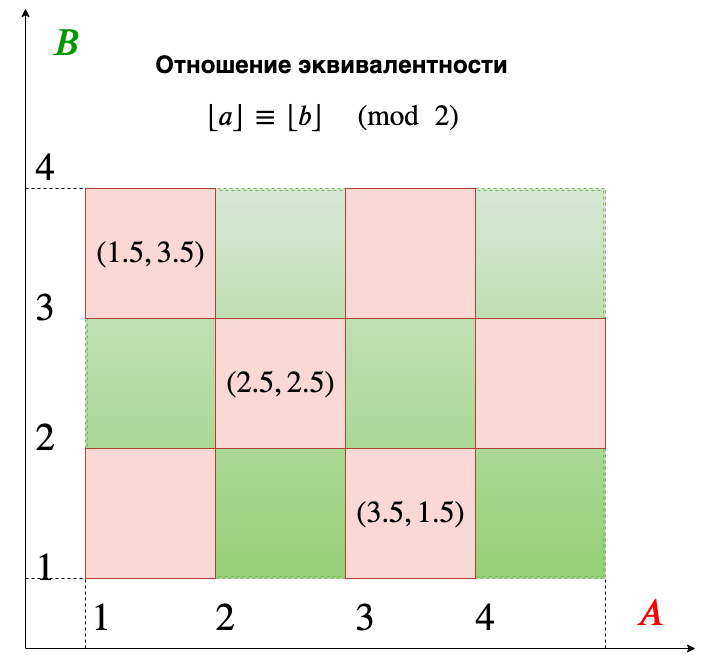
\includegraphics[scale=0.25]{equiv.png}
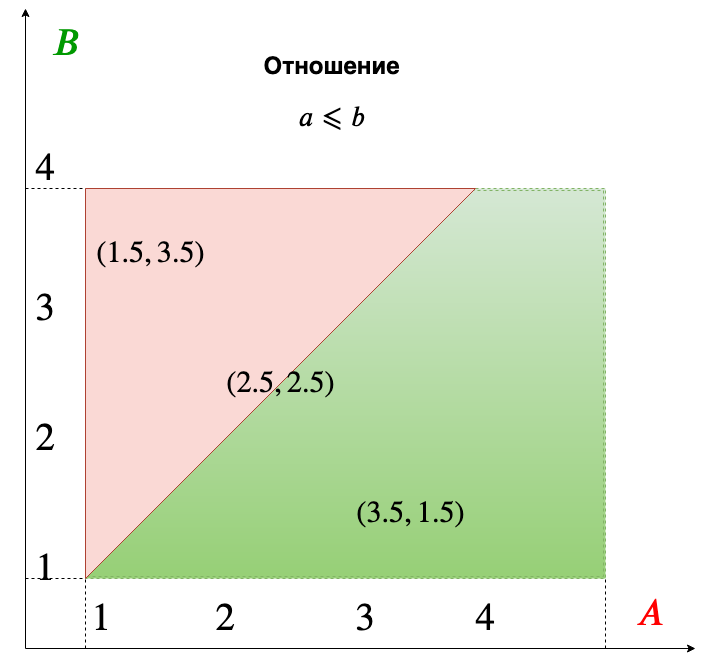
\includegraphics[scale=0.25]{lessthan.png}
\end{center}




\begin{comment}
\chapter{9. Перестановки}
\end{comment}
\newchapter{Перестановки}\label{Permutations}

\vrezka{
В этой главе мы в основном изучаем конечные группы на примере перестановок. Кроме того, изучаются некоторые свойства групп и вводятся необходимые теоретико-множественные определения.
}


\section{Теория множеств: функции}\label{functions}

\lesson{Функция как отношение, инъекция, сюръекция, биекция. Область определения, область значений. Образ и прообраз множества. Обратная функция. Нормальная подгруппа и смежные классы}

\begin{enumerate}
\item Введем понятие функции. Пусть у нас имеется отношение $F$ между множествами $X$ и $Y$. Отношение $F$ называется
\begin{enumerate}[{\bf Func1}]
\item \textbf{всюду значным}, если для каждого $y\in Y$ найдется $x\in X$ такое, что $xFy$;
\item \textbf{всюду определенным}, если для каждого $x\in X$ найдется $y\in Y$ такое, что $xFy$;
\item \textbf{однозначным}, если всякий раз из одновременного выполнения $xFy$ и $xFy'$ следует, что $y=y'$, т.е. каждому $x$ соответствует не более одного $y$;
\item \textbf{обратно однозначным}, если всякий раз из одновременного выполнения $xFy$ и $x'Fy$ следует, что $x=x'$, т.е. каждому $y$ соответствует не более одного $x$;
\item \textbf{функцией из $X$ в $Y$}, если оно всюду определенное и однозначное;\index{Функция}

\item \textbf{сюръекцией из $X$ на $Y$}, если это всюду значимая функция;\index{Функция!сюръекция}
\item \textbf{инъекцией из $X$ в $Y$}, если это обратно однозначная функция;\index{Функция!инъекция}
\item \textbf{биекцией множеств $X$ и $Y$}, если это инъекция и сюръекция одновременно, т.е. отношение $F$ в данном случае взаимно однозначно связывает пары $(x,y)$.\index{Функция!биекция}
\end{enumerate}
Взаимосвязь перечисленных терминов схематично представлена на рис. \ref{function}.

\begin{figure}[hbt!]
\begin{center}
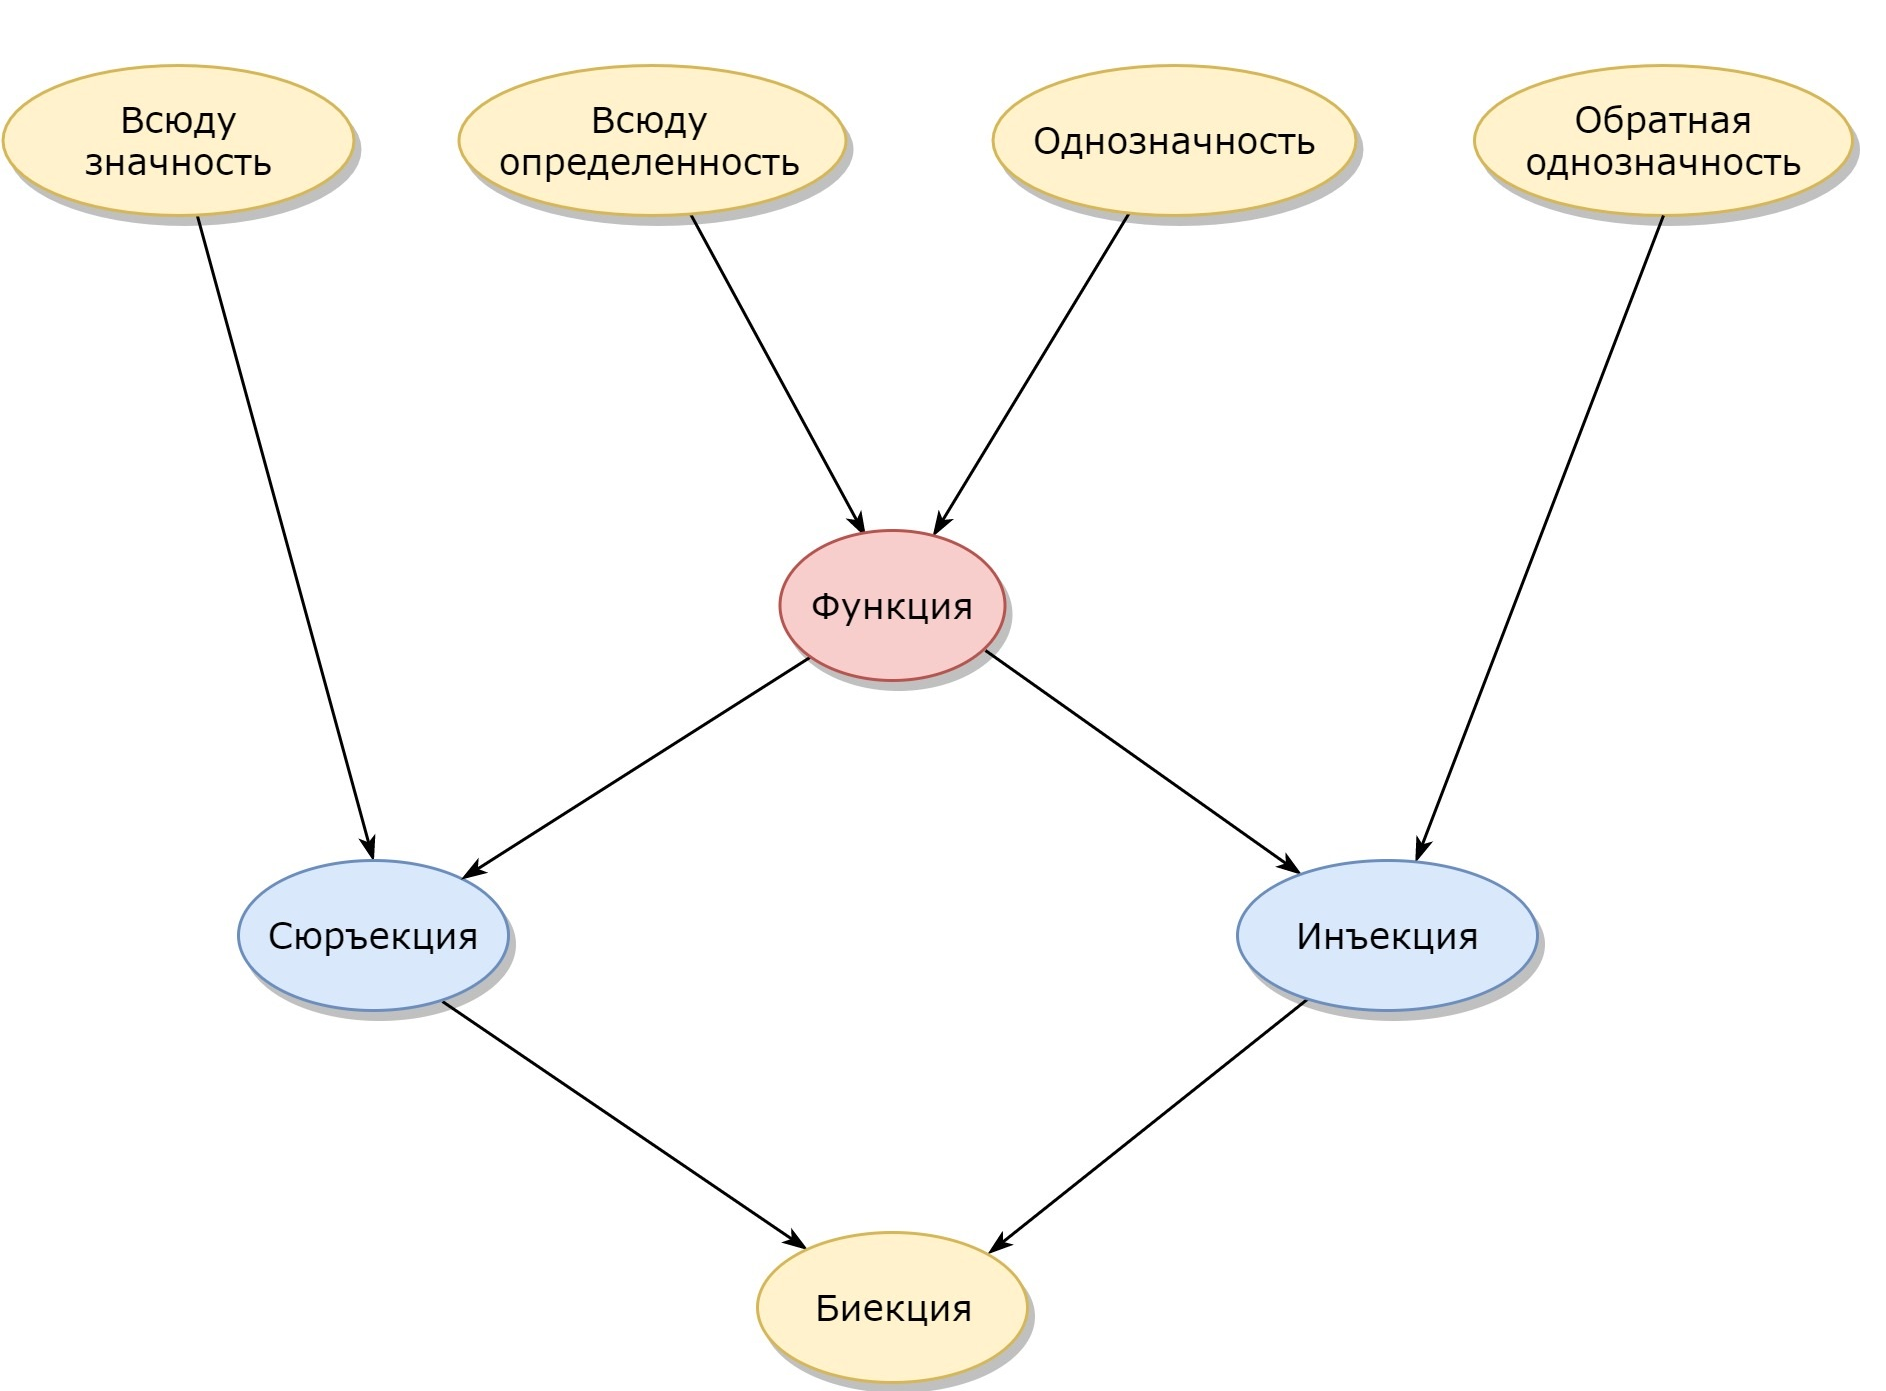
\includegraphics[scale=0.3]{function.png}
\end{center}
\caption{}\label{function}
\end{figure}

Обычно функция из $X$ в $Y$ обозначается $F:X\to Y$, а если $(x,y)\in F$, то пишут $y=F(x)$. Можно также явно определить, что такое $F(x)$, следующим способом:
$$
F(x) = \cup\{y\mid (x,y)\in F\},\quad x\in X.
$$
Поясним. Поскольку функция является однозначным отношением, множество $\{y\mid (x,y)\in F\}$ состоит ровно из одной точки $y$, соответствующей точке $x$ в данном отношении, т.е. оно равно синглету $\{y\}$. А его объединение (т.е. объединение всех его элементов) --- это и есть сам элемент $y$.

Если имеет место равенство $y=F(x)$, то $x$ называют аргументом, а $y$ --- значением функции $F$, соответствующим данному аргументу $x$.

\item Для обозначения биекции часто используется символ $F:X\leftrightarrow Y$.

\item Часто используется термин \textit{частичная функция}, означающий, что функция может быть задана не на всем множестве $X$. Например, функция, которая определена только на простых числах, является частичной функцией, заданной на $\N$. Такая терминология бывает полезной, если используется одно базовое множество, а функции на нем задаются формулами, которые могут быть определены не для всех точек данного множества. Например, на $\Q$ можно рассматривать частичные функции вида $F(x)=1/(x-r)$, где $r\in \Q$. Эти функции будут определены всюду на $\Q$, кроме точки $r$.

Для частичных функций содержательный смысл имеет термин \textit{область определения}, т.е. такое подмножество $X$, где данная функция определена. В случае функции (не частичной) $F:X\to Y$ ее областью определения называется само множество $X$. Область определения функции $F$ принято обозначать $\dom(X)$.

\item Обратным к $F$ отношением называется отношение $F^{-1}=\{(y,x)\mid xFy\}$. Если обратное отношение есть функция, то она называется \textbf{обратной функцией}. Легко видеть, что в том случае, когда существует обратная функция к функции $F$, выполняются равенства $F(F^{-1}(y))=y$ и $F^{-1}(F(x))=x$, если только $F^{-1}(y)$ определено.

Последняя оговорка связана с тем, что обратная функция является частичной функцией из $Y$ в $X$, т.е. она может быт не определена всюду на $Y$, а значит, $F^{-1}(y)$ может не существовать.

\item \textbf{Областью значений} функции $F$ называется подмножество $Y$, обозначаемое $\ran(F)$, для элементов которого $F$ определена, т.е.
$$
\ran(F) = \{y\in Y\mid\exists x\in X\;y=F(x)\}.
$$

\item \textbf{Образом} множества $A\subseteq X$ относительно функции $F$ называется множество\index{Образ}
$$
F[A] = \{y\mid \exists x\in A\;y=F(x)\},
$$
т.е. образ множества --- это результат действия на него функции $F$.

Соответственно, \textbf{прообразом} множества $B\subseteq Y$ называется\index{Прообраз} множество
$$
F^{-1}[B] = \{x\mid F(x)\in B\},
$$
т.е. прообраз множества --- это такое подмножество множества $X$, образ которого лежит в данном множестве $B$. 

Заметим, что для существования прообраза не требуется существования орбратной функции. Кроме того, заметим, что $F[F^{-1}[Y]]$ не всегда равен $Y$.

\item \textbf{Внимание:} Мы намеренно отличаем символы $F(x)$ и $F[A]$, а также $F^{-1}(y)$ и $F^{-1}[B]$, чтобы подчеркнуть, что в случае круглых скобок речь идет о точках (аргумент и значение), а в случае квадратных --- о подмножествах.

\item Итак, функция --- это есть однозначное соответствие элементов одного множества элементам другого (или того же самого). Функции обычно задаются формулами, предписывающими некоторой алгоритм вычисления $y$ через $x$. Но иногда такие формулы не указаны явно или же их указать вовсе невозможно, хотя существование функции строго доказывается (такие теоремы называют теоремами существования).
\end{enumerate}

\subsection*{Задачи}
\begin{enumerate}
\item Рассмотрим соответствие множества людей и множества всех возрастов (целых лет). В каком направлении соответствие между ними является функцией?
\item Рассмотрим соответствие множества людей и банковских счетов. Является ли это соответствие функцией хоть в каком-то направлении?
\item Доказать, что функция $f(x)=3x-7$ биективно отображает $\R$ в $\R$.
\item Доказать, что функция $g(x)=x^2+3x-6$ действует инъективно при $x\in[-3/2,+\infty)$.
\item Докажите, что $F[A\cup C]=F[A]\cup F[C]$ и $F^{-1}[A\cup C]=F^{-1}[A]\cup F^{-1}[C]$.
\item Докажите, что $F[A\cap C]\subseteq F[A]\cap F[C]$ и $F^{-1}[A\cap C]=F^{-1}[A]\cap F^{-1}[C]$.
\item Привести примеры, когда $F[A\cap C]\ne F[A]\cap F[C]$.
\end{enumerate}



\section{Обозначения перестановок}

\lesson{Перестановка, группа перестановок, порядок группы пеерестановок. Теорема Кэли. Циклы}

\begin{enumerate}
\item Рассмотрим множество $X_n=\{x_1,\dots,x_n\}$, состоящее из $n$ элементов, и все возможные биекции множества $X_n$ в себя. Обозначим множество всех биекций за
$$
\Sb(X_n) = \{f\mid f:X_n\leftrightarrow X_n\}.
$$
Проще говоря, $\Sb(X_n)$ --- это множество всех возможных \textbf{перестановок} элементов множества $X_n$.
\item Для функций, заданных на множестве, естественной операцией является операция композиции, т.е. последовательное применение функций. Обычно композиция функций записывается символом $\circ$ или вовсе пропускается. Мы будем пользоваться первым вариантом, так что:
$$
(f\circ g)(x) = f(g(x))
$$
по определению.
\item Итак, мы имеем множество биекций (перестановок) с операцией композиции. Свойства композиции биекций таковы:
\begin{enumerate}[1.]
\item композиция биекций есть снова биекция;
\item $f\circ (g\circ h) = (f\circ g)\circ h$, поскольку это последовательное вычисление $f(g(h(x)))$ при любом $x\in X_n$;
\item существует функция, которая ничего не меняет: $\id(x)=x$, она также является биекцией;
\item для всякой биекции существует обратная функция, которая также является биекцией: $f\circ f^{-1}=f^{-1}\circ f=\id$.
\end{enumerate}

Таким образом, множество $\Sb(X_n)$ (и вообще, $\Sb(X)$ для любого, конечного или бесконечного множества $X$) с операцией композиции является группой. Эта группа называется \textbf{группой перестановок}\index{Группа!перестановок} множества $X_n$, а ее элементы--биекции называются \textbf{перестановками} (или подстановками).\index{Перестановка}


\item Напомним аксиомы группы.\index{Группа}
Пусть на множестве $G$ задана операция $\cdot$ (обозначение которой мы часто будем пропускать для удобства). В терминах функций операция $\cdot$ --- это функция из $G\times G$ в $G$:
$$
\cdot: G\times G\to G.
$$
Тогда пара $(G,\cdot)$ называется \textit{группой}, если:
\begin{enumerate}[G1]
\item $ab\in G$ для всех $a,b\in G$ (группоид);
\item для любых $a,b,c\in G$ имеем тождество $(ab)c=a(bc)$ (ассоциативность);
\item существует элемент $\e\in G$ такой, что $a\e=\e a=a$ для всех $a\in G$ (единица);
\item для всякого $a\in G$ существует обратный элемент $a^{-1}\in G$ такой, что $aa^{-1}=a^{-1}a=\e$ (обратный элемент).
\end{enumerate}
Кроме того, группа называется \textit{абелевой} (или \textit{коммутативной}), если $ab=ba$ для всех $a,b\in G$. Количество элементов в группе называется ее \textbf{порядком}.

Говорят, что функция $f:G_1\to G_2$ является \textbf{изоморфизмом}\index{Изоморфизм групп} групп $(G_1,\circ)$ и $(G_2,\star)$, если $f$ осуществляет взаимно однозначное соответствие обеих групп так, что и результат операций в первой группе переходит в результат операций во второй:
$$
f(g_1\circ g_1') = f(g_1)\star f(g_1').
$$

Например, группа вращений правильного $n$-угольника изоморфна группе вычетов по модулю $n$ с операцией сложения.

Понятие изоморфизма (не только групп, но и более сложных математических структур) является одним из фундаментальных понятий математики. Это --- аналог равенства множеств, но на более высоком уровне, поскольку отвечает за тождество операций и отношений, но пренебрегает тождеством элементов. В Алгебре изоморфные структуры часто просто считаются равными, хотя природа их элементов может кардинально отличаться.

\item Один простой пример группы перестановок мы уже встречали, когда рассматривали все возможные симметрии правильного треугольника. Именно в этом случае все перестановки вершин треугольника соответствовали движениям треугольника, и только они.
\item Сколько всего перестановок в группе $\Sb(X_n)$?

Для ответа на этот вопрос посмотрим, сколько существует вариантов перехода одних элементов в другие. Очевидно, что первый элемент может перейти в любой, в том числе в самого себя, так что для него существует $n$ вариантов. Второй элемент может перейти куда угодно, кроме того места, которое занял первый, так что для него существует $n-1$ вариант. Третьему остается $n-2$ варианта. И т.д. Последнему элементу остается выбор из одного оставшегося места. Таким образом, всего вариантов перестановок на $n$ элементах существует ровно
$$
n(n-1)(n-2)\dots 2\cdot 1=n!
$$
Иначе говоря, группа $\Sb(X_n)$ имеет порядок $n!$.

\item Группа перестановок на трех элементах имеет порядок $3!=6$, что соответствует количеству симметрий правильного треугольника.
Однако уже для квадрата число перестановок равно $24$, в то время как число всех движений составляет всего лишь 8, а для ромба так и вовсе 4. Вообще, как мы помним, количество движений правильного $n$-угольника равно $2n$. С ростом $n$ это число становится во много раз меньше, чем $n!$ (а точнее, в $3\cdot 4\cdots (n-1)=(n-1)!/2$ раз).
\item Чтобы не заострять внимание на происхождении элементов множества $X_n$, обычно они обозначаются числами--символами от $1$ до $n$, а соответствующая группа биекций --- $\Sb_n=\Sb(\{1,2,\dots,n\})$. 

Заметим, что группы $\Sb_n$ и $\Sb(X_n)$ изоморфны, т.е. между ними существует биекция, сохраняющая операцию композиции. Обозначается изоморфизм так: $\Sb_n\isom\Sb(X_n)$.

Для этого достаточно взять произвольную биекцию $H:\{1,2,\dots,n\}\leftrightarrow X_n$ и всякой биекции $f\in\Sb_n$ поставить в соответствие функцию $\bar f$, заданную для всякого $x_i\in X_n$ по правилу
$$
\bar f(x_i) = H(f(H^{-1}(x_i)))\quad (\mbox{т.е. }\bar f=H\circ f\circ H^{-1}).
$$
Изобразим то же самое при помощи диаграммы:
\[ \begin{diagram}
\node{\{1,\dots,n\}}
\arrow[2]{e,t}{f}
\node[2]{\{1,\dots,n\}}
 \arrow{s,r}{H} \\
\node{X_n}
\arrow{n,l}{H^{-1}}
\arrow[2]{e,b}{\bar f=H\circ f\circ H^{-1}}
\node[2]{X_n}
\end{diagram}\]


Нетрудно видеть, что $\bar f:X_n\to X_n$ и что если $x_i\ne x_j$, то $\bar f(x_i)\ne \bar f(x_j)$, поскольку $\bar f$ является композицей трех биекций ($H$, $f$ и $H^{-1}$). Таким образом, $\bar f\in\Sb(X_n)$.

Покажем, что соответствие $f\mapsto\bar f$ является биекцией между $\Sb_n$ и $\Sb(X_n)$, сохраняющей операцию композиции. Пусть $f,g\in \Sb_n$ и $f\ne g$. Это значит, что в некоторой точке $j$ получим $f(j)\ne g(j)$. Но тогда и $\bar f(H(j))\ne \bar g(H(j))$, поскольку $\bar f(H(j))=H(f(j))$ и $\bar g(H(j))=H(g(j))$, а функция $H$ в различных точках принимает различные значения, т.к. является биекцией. То есть, соответствие $f\mapsto\bar f$ разные функции переводит в разные функции. Кроме того, какова бы ни была функция $g\in \Sb(X_n)$, существует $f\in\Sb_n$ такая, что $g=\bar f$. Действительно, пусть $f=H^{-1}\circ g\circ H$, тогда
$$
\bar f = H\circ f\circ H^{-1} = H\circ H^{-1}\circ g\circ H\circ H^{-1} = g.
$$
Итак, соответствие $f\mapsto \bar f$ биективно.

Осталось показать, что оно сохраняет композицию:
$$
\bar{f\circ g} = H\circ (f\circ g)\circ H^{-1} = (H\circ f\circ H^{-1})\circ (H\circ g\circ H^{-1}) =
\bar f\circ \bar g.
$$

Поэтому в дальнейшем, говоря о группе перестановок, мы будем иметь ввиду группу $\Sb_n$, заданную на множестве  $\{1,\dots,n\}$, не акцентируя внимание на природе переставляемых элементов. В свяхи с этим, для удобства дальнейшего изложения положим $X_n=\{1,\dots,n\}$.
\item Теория групп в XIX в. начиналась именно с изучения групп перестановок, и лишь позже понятие группы было обобщено Артуром Кэли. Он же сделал первый важный шаг на пути классификации групп.
\begin{thrm}[Кэли]\index{Теорема!Кэли}
Любая конечная группа порядка $n$ изоморфна некоторой подгруппе $\Sb_n$.
\end{thrm}
\pf 
Пусть $G=\{g_1,\dots,g_n\}$. Для каждого элемента $g_k$ определим функцию $h_k:G\to G$ по правилу:
\begin{equation}\label{hkgk}
h_k(g)=g_kg,\quad g\in G.
\end{equation}
Это --- т.н. <<правые>> биекции, т.к. домножение на аргумент происходит справа. Аналогично можно задать <<левые>> биекции. Легко проверить, что это и в самом деле биекции. Действительно, если $g\ne g'$, то
$h_k(g)\ne h_k(g')$, иначе мы бы получили равенство $g_kg=g_kg'$, и после сокращения на $g_k$ слева получилось бы, что $g=g'$. Таким образом, $h_k$ --- инъекция. Кроме того, для любого $g\in G$ имеем следующее:
$$
h_k(g_k^{-1}g) = g_kg_k^{-1}g=g,
$$
т.е. $h_k$ --- сюръекция и, следовательно, она есть биекция.

Покажем, что множество биекций $H=\{h_1,\dots,h_n\}$ образует группу с операцией композиции. Действительно, 
для любого $g\in G$ имеем $(h_k\circ h_j)(g) = (g_kg_j)g$. А так как $g_kg_j\in G$, то $h_k\circ h_j\in H$. 
Ассоциативность композиции функций выполняется автоматически. Единицей группы $H$ является функция $h_k$ при таком $k$, что $g_k=\e$, т.е. нейтральный элемент группы $G$. Действительно, $h_k(g)=\e g=g$ для всех $g\in G$.
Наконец, обратной функцией к $h_k$ является функция $h(g)=g_k^{-1}g$.

Группа $\Sb(G)$, как мы уже установили, изоморфна группе $\Sb_n$, а значит, группа $H$ изоморфна некоторой подгруппе $\Sb_n$.

Осталось заметить, что $H\isom G$. Это следует из определения элементов $H$. Соответствие $g_k\mapsto h_k$ по формуле \eqref{hkgk} устанавливает изоморфизм этих групп, т.к. произведению $g_kg_j$ соответствует композиция $h_k\circ h_j$.
\epf

\item В группе $\Sb_n$, как и в любой другой конечной группе, можно построить циклическую подгруппу, отправляясь от произвольно взятого элемента, т.\,е. биекции на $X_n$. Например, пусть $s\in\Sb_n$, тогда можно рассмотреть циклическую подгруппу $G(s)=\{s,s^2,s^3,\dots\}$, где под степенью понимается многократная композиция биекции $s$ с самой собою. Ясно, что эта подгруппа не может быть бесконечной, т.\,к. она входит в конечную группу, поэтому при некотором $k$ имеем $s^k=\id$.

\item Рассмотрим некоторую перестановку $s\in \Sb_n$. Ее можно записать в виде таблицы аргумент--значение:
$$
s=
\begin{pmatrix}
1 & 2 & \dots & n-1 & n \\
s_1 & s_2 & \dots & s_{n-1} & s_n
\end{pmatrix}
$$
т.\,е. $s(i)=s_i$. При этом $\{1,2,\dots,n\}=\{s_1,s_2,\dots,s_n\}$ в полном соответствии с определением равенства множеств.

\item Возьмем теперь символ 1 и начнем <<раскручивать>> его:
$$
1\mapsto s(1)\mapsto s(s(1))\mapsto\dots\mapsto s^k(1).
$$
Мы получим то, что называется \textbf{орбитой} элемента 1 при действии группы $G(s)$ на множестве $X_n$. Действительно, все элементы данной цепочки составляют множество $G(s)1=\{g(1)|\;g\in G(s)\}$.

Заметим, что все степени перестановки $s$ являются перестановками, т.е. элементами конечного множества $\Sb_n$. А значит, с ростом $k$ они начнут повторяться, т.е. найдутся такие $k$ и $j$, $k>j$, что $s^k=s^j$. Умножая данное равенство на $s^{-1}$ (обратную к $s$ функцию) достаточное количество раз, мы придем к равенству $s^{k-j}=\id$.
То есть всегда существует такое $k$, что $s^k=\id$.

В этом случае мы получим равенство $s^k(1)=1$, и орбита элемента 1 превратится в \textbf{цикл}:
$$
(1\; s(1)\; s(s(1))\;\dots\; s^{k-1}(1))
$$
(единицу в конце мы не пишем, подразумевая, что последний элемент цикла переходит в первый).

Отметим, что длина цикла в данном случае может оказаться меньше $k$. Например, если перестановка $s$ переводит $1$ в $2$ и $2$ в $1$, но при этом $3$ --- в $4$, $4$ --- в $5$, и $5$ --- в $3$. В таком случае группа $G(s)$ содержит как минимум 6 элементов, в то время как цикл, начинающийся с 1, --- всего лишь два.

\item Действие группы $G(s)$ на множестве $X_n$ позволяет разбить это множество на несколько попарно непересекающихся орбит (или циклов). Покажем это.

Предположим, что орбиты $G(s)1$ и $G(s)2$ имеют общий элемент $j$. Тогда при некоторых натуральных $a,b\le k$ будем иметь $s^a(1)=j=s^b(2)$. Далее, любую степень $s^t(2)$ можно записать в виде:
$$
s^t(2) = (s^{t-b\mod k}\circ s^b)(2) = (s^{t-b\mod k}\circ s^a)(1) = s^{t-b+a\mod k}(1),
$$
где мы использовали вычисления степени по модулю $k$, т.к. $s^k=\id$ и в случае $t<b$ можно добавить $k$ к степени, чтобы выйти на положительную степень.

Таким образом, каждый элемент орбиты $G(s)2$ является элементом орбиты $G(s)1$. Симметрично рассуждая, получаем и обратное вложение, так что $G(s)1=G(s)2$. Аналогично доказывается равенство для любой пары орбит $G(s)j$ и $G(s)l$ в предположении, что у них есть общий элемент. Следовательно, орбиты либо не пересекаются, либо совпадают.

То, что объединение всех орбит равно множеству $X_n$, следует из простого факта, что орбита $G(s)j$ всегда содержит элемент $j$. Итак,
$$
X_n = \bigsqcup_{j=1}^n G(s)j.
$$

Отсюда мы получаем представление самой перестановки $s$ как набора независимых циклов (орбит). Поэтому перестановки принято записывать в виде последовательности циклов. Например, пусть
$$
s=
\begin{pmatrix}
1 & 2 & 3 & 4 & 5 \\
2 & 4 & 1 & 3 & 5
\end{pmatrix}
$$
В этой перестановке мы наблюдаем два цикла: $(1 2 4 3)$ и тривильный $(5)$. Тогда
$$
s=(1 2 4 3)(5),
$$
причем тривиальные циклы принято пропускать в такой <<циклической>> записи, т.\,к. они однозначно восстанавливаются по всем остальным циклам и по параметру $n$ (в нашем случае $n=5$).
\item Рассмотрим более сложный пример:
$$
s=
\begin{pmatrix}
1 & 2 & 3 & 4 & 5 & 6 & 7 \\
2 & 4 & 3 & 1 & 7 & 5 & 6
\end{pmatrix}
=(1 2 4)(3)(5 7 6)=(1 2 4)(5 7 6)
$$

\item Предположим теперь, что у нас имеется три перестановки:
$$
s_1=
\begin{pmatrix}
1 & 2 & 4 \\
2 & 4 & 1
\end{pmatrix};
\quad s_2=
\begin{pmatrix}
5 & 6 & 7 \\
7 & 5 & 6
\end{pmatrix};
\quad s_3=\id.
$$
Тогда исходная перестановка $s$ получается как последовательное применение этих новых перестановок:
$$
s=s_1s_2s_3,
$$
причем порядок перестановок в этой композиции неважен, т.\,к. две из них <<работают>> на разных орбитах, а третья тождественна и коммутирует с любой перестановкой.

\item Таким образом, каждую перестановку из $\Sb_n$ можно единственным образом (с точностью до порядка) представить как композицию циклов, и, таким образом, запись перестановки в виде набора ее циклов является не только удобным соглашением, но еще и функционально полезной.

\end{enumerate}

\subsection*{Задачи}

\begin{enumerate}
\item Пусть $s$ --- некоторая перестановка на $n$ элементах. Для $i,j\in X_n$ запишем $i\sim j$, если существует такое натуральное $k$, что $s^k(i)=j$. Докажите, что
\begin{enumerate}[a)]
\item $\sim$ --- это отношение эквивалентности на множестве $X_n$;
\item классы эквивалентности по данному отношению представляют собой орбиты элементов $X_n$ при действии группы $G(s)$;
\item элементы, входящие в цикл перестановки, составляют класс эквивалентности по отношению $\sim$.
\end{enumerate}
\end{enumerate}



\section{Пара слов о конечных группах}

\lesson{Единственность единицы и обратного элемента, порядок элемента, система образующих, циклическая группа, подгруппа, классы смежности, теорема Лагранжа}


\begin{enumerate}

\item Пусть $G$ --- конечная группа. Приведем некоторые общие свойства групп.

\item В группе существует только одна единица. Действительно, если их две $\e$ и $\e'$, то в силу их же свойств получим
$$
\e' = \e\e' = \e
$$
(при первом равенстве мы рассматривали $\e$ как единицу, а при втором $\e'$).
\item Обратный элемент для каждого $a\in G$ определен однозначно. Предположим, что для элемента $a$ нашлось два обратных элемента $b,c$, т.е. $ab=ba=\e$ и $ac=ca=\e$. Тогда
$$
b=b\e=b(ac)=(ba)c=\e c=c.
$$
\item Степень элемента $\underbrace{a\cdots a}_{k\mbox{ раз}}$ корректно определяется в силу закона ассоциативности и обозначается $a^k$, где $k\in\N$. Кроме того, по определению, $a^0=\e$.
\item Отрицательная степень элемента по определению: $a^{-k}=(a^{-1})^k$, $k\in\N$.
\item Операции со степенями:
$$
(a^k)(a^m)=a^{k+m},
$$
где $k,m\in \Z$. Если $k$ и $m$ одного знака, то это очевидно, а если разного, то пусть $k>0$, $m<0$, тогда
$$
(a^k)(a^m) = \underbrace{a\cdots a}_{k\mbox{ раз}}\underbrace{a^{-1}\cdots a^{-1}}_{|m|\mbox{ раз}}.
$$
Пользуясь ассоциативностью, начинаем сворачивать пары $aa^{-1}$, стоящие в середине, заменяя их на $\e$, а затем выбрасывая $\e$. В итоге либо ничего не останется (когда $k=-m$), либо останутся только $a$ в количестве $k+m$ (если $k>-m$), либо останутся только $a^{-1}$ в количестве $-m-k$ (когда $k<-m$). В любом случае это записывается как $a^{k+m}$ ($(a^{-1})^{-m-k}=a^{m+k}$ по определению).


\item В конечной группе каждый элемент в некоторой конечной степени обращается в $\e$. Действительно, все степени $a^k$ лежат в конечном множестве $G$, а число $k$ пробегает бесконечный науральный ряд. Следовательно, хотя бы два разных $k$ дадут один и тот же элемент (принцип Дирихле): $a^k=a^{k'}$, где $k<k'$. Домножим это равенство на $a^{-k}$ и получим $a^{k'-k}=\e$. Наименьший положительный показатель степени $m$ для элемента $a$, дающий равенство $a^m=\e$, называется порядком элемента $a$ в группе $G$.

Таким образом, в конечной группе у всякого элемента --- конечный порядок.

\item Отсюда следует, что всякую отрицательную степень элемента в конечной группе можно записать как положительную, поскольку
$$
a^k = a^{k\pmod p},
$$
где $p$ --- порядок элемента $a$.

\item Подмножество $T\subseteq G$, все возможные произведения степеней элементов которого, т.е. выражения вида $t_1^{k_1}\cdots t_m^{k_m}$, где $t_j\in T, k_j\in\N$ , образуют всю группу $G$, называется \textbf{системой образующих}\index{Группа!система образующих} или \textbf{порождающим множеством} группы $G$. При этом пишут $G=\langle T\rangle$ или $G=\langle t_1,\dots,t_m\rangle$. Элементы системы образующих называются \textbf{образующими} группы.
\item Если система образующих состоит из одного нетривиального элемента, то группа называется \textbf{циклической}.\index{Группа!циклическая} При этом ее можно записать так: $G=\langle g\rangle$, где $T=\{g\}$. Иначе говоря, циклическая группа состоит из степеней одного своего элемента.
\item Например, группа $\Z/n\Z$ вычетов по модулю $n$ с операцией сложения является циклической: $\Z/n\Z=\langle 1\rangle$, поскольку все ее элементы --- это конечные суммы единиц (от одной до $n$ штук). Группа вращений правильного $n$-угольника является циклической, где образующим элементом является поворот на угол $2\pi/n$. Группа $(\Z/5\Z)^*$, состоящая из элементов $1,2,3,4$, с операцией умножения по модулю 5 является циклической, $(\Z/5\Z)^*=\langle 2\rangle=\langle 3\rangle$.
\item Циклические группы являются абелевыми. Действительно, любые два элемента такой группы --- это некоторые степени образующего элемента, поэтому $(a^k)(a^m)=a^{k+m}=a^{m+k}=(a^m)(a^k)$. Здесь коммутативность наследуется от сложения в группе $\Z$, где $k+m=m+k$.


\item Напомним, что подмножество $H\subseteq G$ называется \textbf{подгруппой} группы $G$, если $H$ само является группой с той же операцией, которая определена в $G$. Например, $\{0,2\}$ образует подгруппу группы $\Z_4$. Тривиальная подгруппа $\{\e\}$ является подгруппой любой группы.

\item Операция Минковского умножения элемента группы на ее подмножество порождает <<смежные классы>>:
$$
gH=\{gh\mid h\in H\},\quad Hg=\{hg\mid h\in H\},
$$
где $gH$ называется левым, а $Hg$ --- правым \textbf{смежным классом} (или классом смежности), порожденным элементом $g\in G$.

\item Классы смежности по данной подгруппе $H$ содержат одинаковое количество элементов.

Действительно, пусть $h_1\ne h_2$, где $h_1,h_2\in H$. Предположим, что $gh_1=gh_2$. Домножая слева на $g^{-1}$, находим, что $h_1=h_2$. Противоречие. Следовательно, умножение на $g$ слева различные элементы переводит в различные. Аналогично --- для умножения справа. Т.о. $|gH|=|Hg|=|H|$ для любой подгруппы $H\subseteq G$ и любого элемента $g\in G$.

\item Классы смежности подгруппы $H$ либо совпадают, либо не пересекаются, а их объединение равно $G$. Иными словами, классы смежности образуют разбиение множества $G$. Такую ситуацию мы уже наблюдали в связи с подгруппами $m\Z$ и их сдвигами внутри $\Z$ и получали там $m$ классов смежности.

Пусть классы $g_1H$ и $g_2H$ имеют общий элемент $g$. Этот элемент будет иметь два представления: $g=g_1h_1=g_2h_2$, где $h_1,h_2\in H$, откуда $g_1=g_2h_2(h_1)^{-1}$. Возмем любой элемент $g_1h$ из первого класса, тогда
$$
g_1h = g_2h_2(h_1)^{-1}h,
$$
где $h_2(h_1)^{-1}h\in H$, т.к. $H$ --- подгруппа. Следовательно, $g_1h\in g_2H$, и $g_1H\subseteq g_2H$. Аналогично рассуждая, находим, что $g_2H\subseteq g_1H$, т.е. $g_1H=g_2H$.

Тот факт, что любой элемент $G$ находится в каком-то классе смежности, следует из того, что $\e\in H$, так что для любого $g\in G$ имеем $g\in gH$. И аналогично для правых классов.

\item Итак, множество $G$ есть объединение непересекающихся классов одного размера, причем размер классов равен порядку подгруппы $H$. Следовательно, порядок подгруппы делит подрядок группы. Это утверждение называется \textbf{теоремой Лагранжа}.\index{Теорема!Лагранжа о порядке группы}


\lesson{Нормальная подгруппа, критерий нормальности подгруппы. Факторгруппа}

\item Подгруппа $H$ группы $G$ называется \textbf{нормальной}\index{Группа!нормальная подгруппа}, если для любого $g\in G$ верно равенство $gH=Hg$, т.е. левые и правые классы не различаются. Обозначение: $H\vartriangleleft G$.

В абелевых группах любая подгруппа будет нормальной. В частности, $m\Z$ --- нормальная подгруппа в $\Z$.

\item Следующее вложение является как критерием нормальности подгруппы, так и, зачастую, используется в качестве ее определения:
\begin{equation}\label{normcriteria}
\forall g\in G\;g^{-1}Hg\subseteq H,\quad (gHg^{-1}\subseteq H).
\end{equation}

Неравенство в скобках равносильно первому, поскольку $g$ --- произвольный элемент $G$, а значит, вместо него можно подставить ему обратный.

Проверим этот критерий. Пусть $H$ --- подгруппа $G$, и выполнено тождество $gH=Hg$ для всех $g\in G$. В частности, это значит, что $Hg\subseteq gH$, т.е.
$$
\forall g\;\forall h\;\exists h'\;(hg=gh')
$$
(не обязательно $h'=h$). Домножая это равенство слева на $g^{-1}$, получаем $g^{-1}hg=h'$, т.е.
$$
\forall g\;\forall h\;(g^{-1}hg\in H),
$$
т.е. $g^{-1}Hg\subseteq H$.

Обратно. Пусть для любого $g\in G$ выполнено вложение $g^{-1}Hg\subseteq H$. То есть, для любых $g\in G$ и $h\in H$ найдется такой $h'\in H$, что $g^{-1}hg=h'$, откуда умножением слева на $g$ получаем $hg=gh'$. Отсюда следует, что $Hg\subseteq gH$.

С другой стороны, $gHg^{-1}\subseteq H$, откуда следует, что для любых $g\in G$ и $h\in H$ найдется такой $h'\in H$, что $ghg^{-1}=h'$, откуда умножением справа на $g$ получаем $gh=h'g$. Отсюда следует, что $gH\subseteq Hg$. 

Окончательно получаем $gH=Hg$.

\item Условие \eqref{normcriteria} равносильно равенству
$$
g^{-1}Hg=H.
$$
Действительно, из этого равенства автоматически следует \eqref{normcriteria}. Поэтому необходимо показать лишь обратное. Выше мы показали, что из \eqref{normcriteria} следует $gH=Hg$. Пусть $h\in H$, тогда
$$
h=(g^{-1}g)h(g^{-1}g)=g^{-1}(ghg^{-1})g=g^{-1}h'g\in g^{-1}Hg,
$$
где $h'\in H$ в силу вложения $gHg^{-1}\subseteq H$. Таким образом, $H\subseteq g^{-1}Hg$, что вместе с вложением \eqref{normcriteria} дает равенство $g^{-1}Hg=H$.


\item Классы смежности нормальной подгруппы можно умножать так же, как сами элементы группы $G$:
\begin{equation}\label{classprod}
(g_1H)(g_2H)=(g_1g_2)H.
\end{equation}
Это следует из того, что $(g_1h_1)(g_2h_2)=g_1(h_1g_2)h_2$, и при этом $h_1g_2=g_2h_3$ при некотором $h_3$ в силу нормальности $H$. Следовательно,
$$
(g_1h_1)(g_2h_2) = g_1(h_1g_2)h_2 = g_1(g_2h_3)h_2=(g_1g_2)(h_3h_2)\in (g_1g_2)H.
$$
Обратно, $(g_1g_2)h=(g_1\e)(g_2h)$. Здесь первый множитель принадлежит $g_1H$, второй $g_2H$. Так что мы имеем взаимное вложение множеств $(g_1H)(g_2H)$ и $(g_1g_2)H$, т.е. их равенство.

\item Такое свойство умножения классов смежности по нормальной подгруппе позволяет задать групповую операцию на множестве всех классов смежности. Действительно, как мы только что установили, произведение классов смежности, заданное по формуле \eqref{classprod}, не выводит из множества классов смежности. Далее, ассоциативность операции напрямую наследуется от такого же свойства операции в группе $G$:
\begin{multline*}
((g_1H)(g_2H))(g_3H)=(g_1g_2)H(g_3)H=((g_1g_2)g_3)H=\\ 
=(g_1(g_2g_3))H=(g_1H)(g_2g_3)H = (g_1H)((g_2H)(g_3H)).
\end{multline*}
Нейтральным элементом является сама подгруппа $H$, т.к. для любого $g\in G$ имеем $(gH)(H)=(g\e)H=gH$ и $(H)(gH)=(\e g)=gH$. Наконец, обратный элемент к $gH$ --- это $g^{-1}H$.

Таким образом, множество классов смежности группы $G$ по нормальной подгруппе $H$ образует группу с операцией умножения \eqref{classprod}. Такая группа обозначается
$$
G/H = \{gH\mid g\in G\}
$$
и называется \textbf{факторгруппой}\index{Группа!Факторгруппа} группы $G$ по нормальной подгруппе $H$. Опять же, мы уже сталкивались с примером фактор-группы $\Z/m\Z$ при изучении группы вычетов (см. раздел \ref{Faktor}).

\item Факторизацию группы можно воспринимать как делимость групп, и в этом смысле группы становятся подобны числам. Есть простые группы --- они ни на что не делятся, а есть составные --- они делятся на нормальные подгруппы.

\item Естественно ввести и умножение групп. Пусть даны две группы $G_1$ и $G_2$ с операциями $\circ$ и $\star$, соответственно. Тогда на прямом произведении $G_1\times G_2$ определим операцию умножения по правилу
$$
(g_1,g_2)(g_1',g_2') = (g_1\circ g_1', g_2\star g_2'),
$$
т.е. будем покомпонентно перемножать все пары элементов прямого произведения. Легко проверить, что это --- групповая операция, т.е. она ассоциативна, имеет единицу, а для каждой пары есть обратная. Все эти свойства наследуются от исходных групп напрямую. Кроме того, если исходные группы абелевы, то и произведение групп будет абелевой группой. Такая конструкция называется внешним \textbf{прямым произведением групп} $G_1$ и $G_2$.

Если в исходных группах операция интерпретируется как сложение или группа является абелевой (например, если речь идет об операции сложения в кольце), то прямое произведение называют \textbf{прямой суммой групп}.


\item Рассмотрим простой пример произведения групп: $\Z_2\times\Z_2$. Вот ее таблица умножения:

\begin{center}
\begin{tabular}{c|cccc}
$\Z_2\times\Z_2$ & 00 & 01 & 10 & 11\\  \hline
00 & 00 & 01 & 10 & 11 \\
01 & 01 & 00 & 11 & 10 \\
10 & 10 & 11 & 00 & 01 \\
11 & 11 & 10 & 01 & 00
\end{tabular}
\end{center}
где вместо пары $(i,j)$ мы просто пишем $ij$ для краткости.

Видим, что эта группа абелева, но не циклическая. В этой группе есть три подгруппы $\{00,01\}$, $\{00,10\}$ и $\{00,11\}$.

Если сравнить ее с группой $\Z_4$ по сложению, то мы увидим существенную разницу. Во-первых, в $\Z_4$ только одна подгруппа $\{0,2\}$, а во-вторых, $\Z_4$ является циклической группой.

Этот пример показывает нам, что порядок группы не определят однозначно ее структуру (как нам того бы хотелось, памятуя об основной теореме арифметики).

Однако нам уже хорошо знакома группа, которая имеет такую же таблицу умножения, как и $\Z_2\times\Z_2$. Это все та же группа симметрий ромба, т.е. четверная группа Клейна. Чуть позже мы к ней вернемся.



\lesson{Классы сопряженности. Критерий нормальности подгруппы через сопряженность}

\item Подгруппа группы $G$ позволяет <<разрезать>> группу $G$ на непересекающиеся классы одинакового размера, которые в случае нормальности подгруппы образуют некоторую новую группу, абстрактуню по отношению к группе $G$. Существуют и другие способы <<разрезания>> группы с помощью чисто групповых приемов. Один из таких способов мы сейчас изучим.

\item Пусть $g,x\in G$, где $G$ --- группа. Элемент $x^{-1}gx$ называется \textbf{сопряженным} к элементу $g$ при помощи $x$. Если сопряженный элемент обозначить как $g^x$, то у нас получаются знакомые свойства:
\begin{enumerate}[1)]
\item $g^{xy}=(g^x)^y$;
\item $(g_1g_2)^x=g_1^xg_2^x$;
\item $(g^{-1})^x=(g^x)^{-1}$;
\end{enumerate}

Действительно,
$$
g^{xy} = (xy)^{-1}g(xy) = y^{-1}(x^{-1}gx)y = y^{-1}(g^x)y = (g^x)^y,
$$
$$
(g_1g_2)^x = x^{-1}(g_1g_2)x = (x^{-1}g_1 x)(x^{-1}g_2x) = g_1^xg_2^x,
$$
$$
(g^{-1})^x = x^{-1}g^{-1}x = (gx)^{-1}(x^{-1})^{-1} = (x^{-1}gx)^{-1} = (g^x)^{-1}.
$$

\begin{lem} Скажем, что $g_1\sim_G g_2$, если при некотором $x$ имеет место равенство $g_1^x=g_2$. Отношение $\sim$ является отношением эквивалентности.
\end{lem}
\pf Рефлексивность: $g=g^\e$. Симметричность: если $g_1^x=g_2$, то $g_2^{x^{-1}}=g_1$. Транзитивность: если $g_1^x=g_2$ и $g_2^y=g_3$, то $g_1^{xy}=g_3$.
\epf

Таким образом, группа $G$ разбивается на классы эквивалентности по отношению $\sim_G$, которые называются \textbf{классами сопряженности}. Класс сопряженности элемента $g$ обозначается $g^G$. Это --- <<сопряжение по Минковскому>>, т.е.
$$
g^G=\{g^x\mid x\in G\}.
$$

На этом, правда, аналогия с классами смежности и заканчивается. Как мы увидим в дальнейшем, классы сопряженности имеют различный размер и могут по-разному соотноситься с классами смежности.


\begin{lem}\label{isomsopr} $g^x$ при фиксированном $x$ является изоморфизмом $G\leftrightarrow G$.
\end{lem}
\pf
Во-первых, $f(g)=g^x$ сохраняет операцию группы $G$, поскольку $f(g_1g_2)=f(g_1)f(g_2)$. Во-вторых, это мономорфизм (инъекция с сохранением операции), т.е. если $x^{-1}g_1x=x^{-1}g_2x$, то $g_1=g_2$. В-третьих, это эпиморфизм (сюръекция с сохранением операции), т.к. для любого $g\in G$ найдется $g'$ такой, что $g=f(g')$, а именно, $g'=xgx^{-1}$.
\epf

Итак, при каждом $x$ функция $f(g)=g^x$ задает изоморфизм группы $G$ на себя. Такой изоморфизм называется \textbf{автоморфизмом} группы $G$.\index{Автоморфизм группы} Множество всех автоморфизмов группы $G$ принято обозначать $\Aut(G)$.

\item Классы сопряженности напрямую связаны с нормальными подгруппами.
\begin{thrm}\label{normcrit2}\index{Подгруппа!критерий нормальности}
Подгруппа $H$ группы $G$ является нормальной тогда и только тогда, когда она есть объединение нескольких классов сопряженности.
\end{thrm}
\pf
Пусть $H\vartriangleleft G$, тогда $H=x^{-1}Hx$ для любого $x\in G$. Тогда вместе с любым элементом $h\in H$ имеем вхождение всего класса $h^G\subseteq H$. То есть, если класс сопряженности пересекается с нормальной подгруппой, то он входит в нее целиком. Отсюда следует, что нормальная подгруппа является объединением классов сопряженности (не обязательно всех).

Обратно, пусть подгруппа $H=g_1^G\cup\dots\cup g_n^G$. Операция сопряжения сохраняет классы сопряженности:
$$
x^{-1}g^Gx=\{x^{-1}g^yx\mid y\in G\} = \{g^{yx}\mid y\in G\}=g^G.
$$
Последнее равенство справедливо, поскольку элемент $yx$ --- произвольный элемент $G$, т.е. для любого $z\in G$ имеем $z=yx$ при $y=zx^{-1}$.

Тогда получаем, что
$$
x^{-1}Hx=x^{-1}g_1^Gx\cup\dots\cup x^{-1}g_n^Gx =g_1^G\cup\dots\cup g_n^G=H,
$$
откуда следует, что подгруппа $H$ является нормальной.
\epf

Отметим, что произвольное объединение классов сопряженности не обязано быть подгруппой, а значит, и нормальной подгруппой. Однако нормальные подгруппы следует искать только среди таких объединений, что сильно упрощает их поиск. Важно, чтобы эти объединения оказались замкнутыми относительно групповой операции! Поэтому такое объединение должно включать как минимум тривиальный класс $\{\e\}$.
\end{enumerate}




\section{Знакопеременная группа}

\lesson{Транспозиция. Определение четности, теорема о корректности определения}

\begin{enumerate}
\item Мы введем теперь такое важное понятие как \textbf{транспозиция}. Это --- микроцикл, состоящий из двух элементов, например, (12) или (59) и т.п. Транспозиция меняет местами два элемента $X_n$, а остальные оставляет на месте. Любой цикл длины $k$ можно представить как композицию $(k-1)$ транспозиции. Например,\label{transpose}\index{Транспозиция}
$$
(1234) = (14)(13)(12),
$$
причем это представление неоднозначное, поскольку, например,:
$$
(1234) = (2341) = (21)(24)(23),
$$
тем не менее, любая перестановка (не только цикл) имеет \textit{инвариант} по разложению в транспозиции.
\begin{thrm}
Если перестановка $s\in\Sb_n$ имеет два представления транспозициями
$$
s=t_1\dots t_k=\tau_1\dots\tau_m,
$$
то $k\equiv m\mod 2$.
\end{thrm}
\pf
Пусть дана некоторая перестановка $s$ на $n$ элементах. Запишем ее в виде матрицы
$$
s=\begin{pmatrix}
1 & 2 & \dots & n \\
s_1 & s_2 & \dots & s_n
\end{pmatrix},
$$
где $s_1,\dots, s_n\in\{1,\dots,n\}$ попарно различны. Для такой перестановки $s$ рассмотрим функцию
\begin{equation}\label{DeltaS}
\De(s) = \prod_{i<j}(s_j-s_i),
\end{equation}
т.е. находим все <<подъемы>> и <<спуски>> нашей перестановки. Например, $\De(123)=(2-3)(2-1)(3-1)$. Иными словами, мы перемножаем все возможные разности пар элементов перестановки, вычисляя разность в обратном порядке следования индексов: если функция $s$ растет на паре индексов $ij$, то разность будет положительной.

Посмотрим, что происходит с функцией $\De$, если перестановку $s$ умножить на произвольную транспозицию $(ij)$, где $i<j$. Во-первых,
$$
s' = s\circ (ij) = \begin{pmatrix}
1 & 2 & \dots & i & \dots & j & \dots & n \\
s_1 & s_2 & \dots & s_j & \dots & s_i & \dots & s_n
\end{pmatrix},
$$
т.е. $s_i$ поменялось местами с $s_j$: $s'_i=s_j$, $s'_j=s_i$, а остальные элементы остались на своих местах: $s'_k=s_k$ для всех $k\notin\{i,j\}$. 

Во-вторых, рассмотрим отношение $\De(s)/\De(s\circ(ij))$. В числителе и знаменателе стоят одни и те же разности, только местами отличающиеся знаком. Поэтому для нахождения данного отношения нужно лишь найти количество таких перемен знаков в этих разностях.

Рассмотрим все возможные пары индексов и соответствующие им разности, входящие в функции $\De(s)$ и $\De(s\circ(ij))$, включающие и не включающие индексы $i$ и $j$:
\begin{itemize}
\item $(s'_j-s'_i)=(s_i-s_j)=(-1)(s_j-s_i)$, т.е. в данном случае происходит смена знака сомножителя для пары индексов $ij$;
\item при $k>j$ получаем, что $(s'_k-s'_j)(s'_k-s'_i)=(s_k-s_i)(s_k-s_j)$, т.е. для двух пар индексов $ik$ и $jk$ произведение соответствующих разностей не меняется (отличие только в порядке множителей), и смены знака нет;
\item при $k<i$ получаем, что $(s'_j-s'_k)(s'_i-s'_k)=(s_i-s_k)(s_j-s_k)$, т.е. для двух пар индексов $ki$ и $kj$ произведение соответствующих разностей тоже не меняется;
\item при $i<k<j$ получаем, что $(s'_k-s'_i)(s'_j-s'_k)=(s_k-s_j)(s_i-s_k)=(-1)(s_j-s_k)(-1)(s_k-s_i)$, и снова произведение разностей для пар индексов $ik$ и $kj$ не меняется (хотя обе разности сменили знак);
\item для всех остальных пар индексов $kl$, где $k<l$ и $k,l\notin\{i,j\}$, разность $s_l-s_k$ сохраняется.
\end{itemize}
Таким образом, функции $\De(s)$ и $\De(s\circ(ij))$ содержат одинаковые разности, некоторых из которых отличаются знаком, причем во всех случаях, кроме одного, знак либо не меняется, либо смена знака одной разности компенсируется сменой знака другой разности. А значит, отношение $\De(s)/\De(s\circ(ij))$ равно $-1$.

Пусть теперь $s=\id$, т.е. $s_k=k$ при всех $k\in\{1,\dots,n\}$. Тогда все разности $(s_j-s_i)=j-i$ положительны, т.е. $\De(\id)>0$.

Отсюда следует, во-первых, что \textit{композиция тождественной перестановки и транспозиции не может быть тождественной перестановкой}, поскольку $\De(\id\circ(ij))=-\De(\id)$. А во-вторых, знак функции $\De(s)$ определяется выражением $(-1)^k$, где $k$ --- количество транспозиций в разложении перестановки $s$.

Отсюда следует, что если имеет место представление
$$
s=t_1\dots t_k=\tau_1\dots\tau_m,
$$
то $(-1)^k=(-1)^m$, а это возможно только в том случае, когда $k\equiv m\mod 2$. Теорема доказана.
\epf

Данная теорема позволяет корректно определить понятие четности (или знака) перестановки. А именно, знак функции $\De(s)$ называется \textbf{четностью перестановки} $s$ и обозначается $\sgn(s)$, причем если этот знак положительный, то перестановка $s$ называется \textbf{четной}, а в противном случае --- \textbf{нечетной}. И, как мы выяснили в ходе доказательства теоремы, четность перестановки $s$ равна $(-1)^k$, где $k$ --- количество транспозиций в разложении $s$, и не зависит от конкретного представления $s$ в виде композиции транспозиций. В частности, $\sgn(\id)=+1$, $\sgn(ij)=-1$. 

Кроме того, из определения функции $\De(s)$ по формуле \eqref{DeltaS} видно, что \textit{четность перестановки  определяется количеством инверсий данной перестановки}. \textbf{Инверсией} называется такая пара индексов $ij$, что $s_j<s_i$, т.е. когда перестановка меняет отношение порядка. Если $k$ --- количество инверсий перестановки $s$, то $\sgn(s)=(-1)^k$. Таким образом, \textit{четность перестановки совпадает с четностью количества ее инверсий}.



\lesson{Гомоморфизм, ядро гомоморфизма}

\item Отметим одно важно свойство $\sgn(s)$. Пусть заданы две перестановки $s$ и $g$. Запишем их в виде композиции транспозиций
$$
s=t_1\dots t_k,\quad g=\tau_1\dots\tau_m.
$$
Тогда четность композиции $sg$ будет равна $(-1)^{k+m}$, поскольку $sg=t_1\dots t_k\tau_1\dots\tau_m$. Таким образом,
\begin{equation}\label{sgnsgn}
\sgn(sg)=\sgn(s)\sgn(g).
\end{equation}
\item В связи с таким свойством функции четности перестановки уместо дать следующее важное определение.
\textbf{Гомоморфизмом группы}\index{Гомоморфизм} $(G,\cdot)$ в группу $(G',\circ)$ называется любая функция $h:G\to G'$, сохраняющая групповую операцию, т.\,е.
$$
h(g_1\cdot g_2)=h(g_1)\circ h(g_2),\quad g_1,g_2\in G.
$$

\item Функция $\sgn$, определенная на элементах группы $\Sb_n$ и принимающая значения из множества $B=\{-1,1\}$, является гомоморфизмом группы $\Sb_n$ в группу $B$ (проверьте, что $(B,\cdot)$ есть группа по умножению, изоморфная $\Z_2$), поскольку в силу \eqref{sgnsgn} функция $\sgn$ композиции перестановок ставит в соответствие произведение их знаков.

\item \textbf{Ядром гомоморфизма}\index{Ядро гомоморфизма} $h$ называется прообраз единицы:
$$
\Ker(h)= h^{-1}[\{\e'\}]=\{g\in G|\;h(g)=\e'\},
$$
где $\e'$ --- единица группы $G'$.

Гомоморфизм обладает следующими свойствами:
\begin{enumerate}[\bf Hom1]
\item Единицу переводит в единицу. Действительно, пусть $h(\e)=g'$. Тогда
$$
g'=h(\e)=h(\e\e)=h(\e)h(\e)=g'g',
$$
откуда, используя сокращение в группе $G'$, получаем, что $\e'=g'$.

\item Обртаный элемент переводит в обратный. Пусть $g'=h(g)$ и $g''=h(g^{-1})$, тогда
$$
g'g'' = h(g)h(g^{-1})=h(gg^{-1})=h(\e)=\e',\quad g''g'=\e',
$$
т.е. элемент $g''$ --- обратный к $g'$, или $h(g^{-1})=h(g)^{-1}$.

\item Ядро гомоморфизма есть нормальная подгруппа: $\Ker(h)\vartriangleleft G$.

Проверим аксиомы группы. Пусть $g_1, g_2\in \Ker(h)$, тогда $h(g_1g_2)=h(g_1)h(g_2)=\e'$, откуда $g_1g_2\in\Ker(h)$, т.е. ядро замкнуто относительно групповой операции в $G$. Ассоциативность наследуется из $G$. Единица находится в ядре, согласно Hom1.

Пусть $g\in\Ker(h)$, тогда $h(g^{-1})=h(g)^{-1}=(\e')^{-1}=\e'$, откуда $g^{-1}\in\Ker(h)$. Таким образом, все требования группы выполнены, и $\Ker(h)$ является подгруппой в $G$. Проверим ее нормальность.

Пусть $g\in G$ и $k\in\Ker(h)$, тогда $h(g^{-1}kg)=h(g)^{-1}h(k)h(g)=h(g)^{-1}\e'h(g)=\e'$. Отсюда следует, что $g^{-1}kg\in\Ker(h)$, т.е. $g^{-1}\Ker(h)g\subseteq \Ker(h)$.

А это, по доказанному ранее критерию нормальности \eqref{normcriteria}, означает, что $\Ker(h)\vartriangleleft G$.

\end{enumerate}

\item Поскольку функция $\sgn$ на группе $\Sb_n$ действует как гомоморфизм в группу $B$, прообраз 1 в группе $\Sb_n$ относительно данного гомоморфизма, а именно, \textit{все четные перестановки}, образуют нормальную подгруппу в группе  $\Sb_n$. Эта нормальная подгруппа обозначается $A_n$ и называется \textbf{знакопеременной группой}\index{Группа!знакопеременная} порядка $n$. Не следует путать употребленное здесь слово <<порядок>> с порядком группы, означающим количество ее элементов, поскольку в $A_n$ находится ровно половина элементов группы $\Sb_n$, т.\,е. $n!/2$, что значительно больше $n$ при $n>3$.

\end{enumerate}



\section{Структура группы перестановок}

\lesson{Классы сопряженности в $\Sb_3$ и $\Sb_4$. Нормальные подгруппы групп $\Sb_3$ и $\Sb_4$. Ипостаси четверной группы Клейна}


\begin{enumerate}


\item Посмотрим, как работает отношение сопряженности на группе перестановок.

Пусть $G=\Sb_3 = \{\id,(12),(13),(23),(123),(132)\}$. Будем записывать действие $g^x$ в виде таблицы, похожей на таблицу умножения, предполагая, что на верхнюю строку мы действуем функцией $g^x$, где $x$ берется из левого столбца:
\begin{center}
\begin{tabular}{c|c|ccc|cc}
${}_x\setminus^g$&  $\id$	& (12)	& (13)	& (23)	& (123)	& (132) \\ \hline
$\id$&$\id$	& (12)	& (13)	& (23)	& (123)	& (132) \\
(12)& $\id$	& (12)	& (23)	& (13)	& (132)	& (123) \\
(13)& $\id$	& (23)	& (13)	& (12)	& (132)	& (123) \\
(23)& $\id$	& (13)	& (12)	& (23)	& (132)	& (123) \\
(123)&$\id$	& (23)	& (12)	& (13)	& (123)	& (132) \\
(132)&$\id$	& (13)	& (23)	& (12)	& (123)	& (132)
\end{tabular}
\end{center}
Мы видим, что когда $x$ есть транспозиция, то сопряжение к $g$ при помощи $x$ --- это либо само $g$ (а именно, при $g=x$, т.к. $x^x=x$), либо другая перестановка того же вида: сопряжением к транспозиции является транспозиция, а спопряжением к 3-циклу --- 3-цикл. Если же $x$ --- это 3-цикл, то сопряжением к транспозиции является обязательно другая транспозиция, а сопряжением к 3-циклу является он сам.

Коме того, каждая строка таблицы --- это перестановка элементов группы $\Sb_3$ (в соответствии с леммой \ref{isomsopr} это не просто перестновка, а автоморфизм группы $\Sb_3$). Эту перестановку можно также рассматривать как элемент группы $\Sb(\Sb_3)$, изоморфной группе $\Sb_6$.

Перестановки элементов группы $\Sb_3$, получаемые их сопряжением, подчиняются строгим ограничениям. Мы специально разделили таблицу на три части, включив в первую $\id$, во вторую --- транспозиции, а в третью --- 3-циклы. Такое разделение соответствует найденному нами выше 
разбиению на классы сопряженности по
отношению эквивалентности $\sim_G$ (в нашем случае это $\sim_{\Sb_3}$). И действительно, если смотреть теперь на столбцы таблицы, то внутри каждого столбца мы видим только элементы, сопряженные друг другу.

Мы можем построить аналогичную таблицу для $\Sb_4$ и убедиться в том, что (a) каждая строка таблицы есть перестановка элементов $\Sb_4$ и (b) каждый столбец --- выборка с повторениями из соответствующих классов сопряженности. Таковыи классами для $\Sb_4$ являются классы одинакового цикленного состава:

\begin{tabular}{c|l|c}
()    & $\id$ & 1 \\
(**)   & (12),(13),(14),(23),(24),(34) & 6 \\
(***)  & (123),(132),(124),(142),(134),(143),(234),(243) & 8\\
(**)(**) & (12)(34), (13)(24), (14)(23) & 3 \\
(****) & (1234),(1243),(1324),(1342),(1423),(1432) & 6
\end{tabular}


Эти классы можно обозначить как $\id^{\Sb_4}$, $(12)^{\Sb_4}$, $(123)^{\Sb_4}$, $[(12)(34)]^{\Sb_4}$, $(1234)^{\Sb_4}$.

На самом деле, для любой группы $\Sb_n$ классы сопряженности состоят из перестановок одинакового цикленного состава (т.е. совпадает количество циклов одинаковой длины).


\item В группе $\Sb_3$ есть только две возможности создать нетривиальную нормальную подгруппу: на основе класса $(12)^{\Sb_3}$ и на основе класса $(123)^{\Sb_3}$. Но в первом случае подгруппа не получается, поскольку $(12)(23)=(123)$ выходит из класса транспозиций. Зато второй случай позволяет создать уже знакомую нам знакопеременную подгруппу, состоящую из всех четных перестановок на 3-х символах:
$$
A_3 = \{\id,(123),(132)\}.
$$
По доказанной теореме \ref{normcrit2} она является нормальной.

\item В группе $\Sb_4$ возможностей сильно больше, но далеко не все они приводят к подгруппе. Вспомним, что порядок подгруппы делит порядок группы (теорема Лагранжа). Следовательно, собственные нетривиальные подгруппы $\Sb_4$ должны иметь порядок из множества $\{2,4,6,8,12\}$. А перечисленные выше классы сопряженности имеют размеры 1,6,8,3,6. И так как подгруппа должна включать класс $\{\id\}$, ее порядок может скадываться только следующими двумя способами: $1+3$, $1+3+8$. И действительно, в группе $\Sb_4$ существует ровно две нетривиальные собственные нормальные подгруппы:
\begin{align*}
V_4 = & \{\id,(12)(34),(13)(24),(14)(23)\},\\
A_4 = & \{\id,(12)(34),(13)(24),(14)(23), \\
      & \;(123),(132),(124),(142),(134),(143),(234),(243)\}
\end{align*}
Первая --- это уже известная нам четверная группа Клейна, которая изоморфна группе симметрий ромба, группе $\Z_8^*$ и группе $\Z_2\times\Z_2$. Можно построить гомоморфизм из $\Sb_4$ в $\Sb_3$ с ядром $V_4$. У этого факта существует простое геометрическое доказательство. Дело в том, что группа $\Sb_4$ является группой симметрий тетраэдра (включая отражения), тогда, если в тетраэдре соединить середины противоположных ребер, получится три отрезка. При движениях тетраэдра движутся и эти отрезки, переходя друг в друга, и эти движения образуют группу, изоморфную $\Sb_3$. При этом, как легко проверить, движения вершин тетраэдра, соответствующие перестановкам из группы Клейна, не меняют положение этих отрезков (они могут переворачиваться, но переходят каждый сам в себя), т.е. группа Клейна является ядром такого гомоморфизма. Из основной теоремы о гомоморфизмах также следует, что $\Sb_4/V_4$ изоморфна $\Sb_3$, поскольку $\Sb_3$ --- образ гомоморфизма с ядром $V_4$.

Вторая --- подгруппа $A_4$ --- это знакопеременная подгруппа, содержащая все четные перестановки на 4-х символах, и только их.

\item Соберем известные нам группы 4го порядка в одну таблицу \ref{vier} для сравнения.

\begin{table}[h!]
\begin{tabular}{c||c}
Четверная группа Клейна & Циклическая 4-го порядка \\ \hline\hline
\\

\begin{tabular}{c|cccc}
$\Diamond$ & $\id$     & $R$   & $S_1$ & $S_2$ \\ \hline
     $\id$ & $\id$     & $R$   & $S_1$ & $S_2$ \\ 
     $R$   & $R$       & $\id$ & $S_2$ & $S_1$ \\
     $S_1$ & $S_1$     & $S_2$ & $\id$ & $R$ \\
     $S_2$ & $S_2$     & $S_1$ & $R$   & $\id$
\end{tabular}
 & \footnotesize
\begin{tabular}{c|cccc}
$\Box$ & $\id$ & $R_{\pi/2}$ & $R_{\pi}$ & $R_{3\pi/2}$ \\[1pt]  \hline \\[-6pt]
$\id$  & $\id$ & $R_{\pi/2}$ & $R_{\pi}$ & $R_{3\pi/2}$ \\[3pt]
$R_{\pi/2}$  & $R_{\pi/2}$ & $R_{\pi}$ & $R_{3\pi/2}$ & $\id$ \\[3pt]
$R_{\pi}$ & $R_{\pi}$ & $R_{3\pi/2}$ & $\id$ & $R_{\pi/2}$\\[3pt]
$R_{3\pi/2}$ & $R_{3\pi/2}$ & $\id$ & $R_{\pi/2}$ & $R_{\pi}$
\end{tabular}
\\

\\


\begin{tabular}{c|cccc}
$\Z_8^*$ & 1 & 3 & 5 & 7 \\  \hline
1 & 1 & 3 & 5 & 7 \\
3 & 3 & 1 & 7 & 5\\
5 & 5 & 7 & 1 & 3\\
7 & 7 & 5 & 3 & 1
\end{tabular}
 &
\begin{tabular}{c|cccc}
$\Z_4$ & 0 & 1 & 2 & 3 \\  \hline
0 & 0 & 1 & 2 & 3 \\
1 & 1 & 2 & 3 & 0\\
2 & 2 & 3 & 0 & 1\\
3 & 0 & 1 & 2 & 3
\end{tabular}
\\

\\


\begin{tabular}{c|cccc}
$\Z_2\times\Z_2$ & 00 & 01 & 10 & 11\\  \hline
00 & 00 & 01 & 10 & 11 \\
01 & 01 & 00 & 11 & 10 \\
10 & 10 & 11 & 00 & 01 \\
11 & 11 & 10 & 01 & 00
\end{tabular}
 &
\begin{tabular}{c|cccc}
$\Z_5^*$ & 1 & 2 & 4 & 3 \\  \hline
1 & 1 & 2 & 4 & 3 \\
2 & 2 & 4 & 3 & 1\\
4 & 4 & 3 & 1 & 2\\
3 & 3 & 1 & 2 & 4
\end{tabular}
\\
\\

\footnotesize %\sffamily
\begin{tabular}{cc|cc}
 $\id$    & (12)(34) & (13)(24) & (14)(23) \\[5pt]
 (12)(34) & $\id$    & (14)(23) & (13)(24) \\[3pt]\hline
 &&& \\[-5pt]
 (13)(24) & (14)(23) & $\id$    & (12)(34) \\[5pt]
 (14)(23) & (13)(24) & (12)(34) & $\id$
\end{tabular}
 &
\begin{tabular}{c|cccc}
$\sqrt[4]{1}$ & 1    & $i$  & $-1$ & $-i$ \\  \hline
1             & 1    & $i$  & $-1$ & $-i$ \\
$i$           & $i$  & $-1$ & $-i$ & 1    \\
$-1$          & $-1$ & $-i$ & 1    & $i$  \\
$-i$          & $-i$ & 1    & $i$  & $-1$
\end{tabular}
\\
\\

\hline

\end{tabular}
\caption{}\label{vier}
\end{table}

Отметим, что с точностью до изоморфизма существует всего две группы 4-го порядка: группа Клейна и циклическая группа. Несмотря на все разнообразие их представителей!


\lesson{Игра <<Пятнадцать>>. Инварианты. Нормальный ряд, разрешимость. Анонс теории Галуа}


\subsection*{Игра <<Пятнадцать>>}


\item Четность перестановки является инвариантом на подгруппе $A_n$ (т.е. принимает одно и то же значение на всех ее элементах), а также на ее смежном классе в $\Sb_n$ (принимает другое постоянное значение). Поиск инвариантов является одним из мощных математических инструментов при поиске закономерностей и доказательстве невозможности некоторых объектов или действий.

\item С конца XIX века известна игра <<пятнадцать>>, суть которой в следующем. Имеем поле 4x4, в котором расставлены одинаковые по размеру фишки размером 1x1. Всего фишек 15, и они пронумерованы числами от 1 до 15. Одно место на поле пустое, что позволяет производить следующие простые манипуляции: занимать данное место фишкой с любого смежного места, т.\,е. передвигать ее на это место, освобождая соседнее.
При этом нельзя совершать никакие другие действия, например, вынимать фишки с поля и расставлять их произвольным образом.

В результате таких действий порядок номеров у фишек меняется, т.\,е. мы осуществляем перестановку из группы $\Sb_{15}$.

<<Фишка>> этой игры в том, что все разрешенные манипуляции не меняют четности исходной перестановки номеров. А это значит, что никакую нечетную изначальную расстановку невозможно привести (разрешенными действиями) к четной перестановке, и наоборот. Например, две расстановки фишек, отличающиеся лишь одной транспозицией (обменом двух соседних фишек местами), не могут быть переведены одна в другую.

Создатель игры (никто еще не знал тогда алгебраического решения задачи) даже обещал приз 100 долларов тому, кто приведет расстановку
\begin{center}
\begin{tabular}{|c|c|c|c|}
\hline
1 & 2 & 3 & 4 \\ \hline
5 & 6 & 7 & 8 \\ \hline
5 & 6 & 7 & 8 \\ \hline
9 & 10 & 11 & 12 \\ \hline
13 &15 & 14 & \\ \hline
\end{tabular}
\quad к виду \quad
\begin{tabular}{|c|c|c|c|}
\hline
1 & 2 & 3 & 4 \\ \hline
5 & 6 & 7 & 8 \\ \hline
5 & 6 & 7 & 8 \\ \hline
9 & 10 & 11 & 12 \\ \hline
13 &14 & 15 & \\ \hline
\end{tabular}
\end{center}
(они отличаются транспозицией (15\ 14)).

С тех пор прошло больше 100 лет, и до сих пор многие пытаются это сделать, но алгебра дает нам беспощадный ответ: это сделать невозможно! Потому что четность перестановки инвариантна относительно действий с фишками!

\item Другой замечательный пример инварианта --- теорема Эйлера о числе выпуклого многогранника: величина В-Р+Г=2 для всех выпуклых многогранников (В --- число вершин, Р --- ребер, Г --- граней). Отсюда, в частности, следует, что на футбольном мяче, сшитом только из правильных 5- и 6-угольников, может быть только 12 пятиугольников, никакое другое число не удовлетворяет этому инварианту.


\subsection*{Нормальный ряд}

\item Выше мы отыскали все нормальные подгруппы $\Sb_3$ и $\Sb_4$. В таблице \ref{SymmetricS4} (в конце книги) помещена полная таблица умножения группы $\Sb_4$ с использованием кратких обозначений перестановок как произведений циклов. Там же выделены две подтаблицы, отвечающие группам $A_4$ и $V_4$, а также отмечены (жёлтым) элементы (и их произведения) некоторой подгруппы 8-го порядка, которая не является ни нормальной, ни абелевой (и поэтому она не является суммой классов сопряженности).

Выделенная подгруппа 8-го порядка:
$$\{\e, (12)(34), (13)(24), (14)(23), (12), (34), (1324), (1423)\}.
$$
Все подгруппы 8-го порядка изоморфны. Аналогичная ситуация с подгруппами 6-го порядка, вот одна из них:
$\{\e, (123), (132), (12), (13), (23) \}$, которая совпадает с $\Sb_3$.

\item В группе $\Sb_4$ существует только 2 нетривиальные нормальные подгруппы: $A_4$ и $V_4$. Все подгруппы порядков 2,3,6,8 не являются нормальными.

\item Говорят, что группа $G$ имеет \textbf{субнормальный ряд} (называемый также \textbf{субнормальной башней}, \textbf{субинвариантным рядом}, \textbf{субнормальной матрёшкой} или просто \textbf{рядом}) длины $n$, если имеют место вложения:
$$
\{\e\}=G_0\vartriangleleft G_1\vartriangleleft\dots\vartriangleleft G_{n-1}\vartriangleleft G_n=G,
$$
где $G_i$ --- собственная нормальная подгруппа в $G_{i+1}$. Ряд называется \textbf{нормальным}, если все $G_i$ нормальны также в исходной группе $G$. Факторгруппы $G_{i+1}/G_i$ называются \textbf{факторами} (факторгруппами) \textbf{ряда}.

Для простых групп (например, $\Z_p$) тривиальный субнормальный ряд длины 1 является единственно возможным: $\{\e\}\vartriangleleft G$.

Для группы $\Sb_4$ имеем: 
$$
\{\e\}\vartriangleleft V_4\vartriangleleft A_4\vartriangleleft\Sb_4,\quad\{\e\}\vartriangleleft V_4\vartriangleleft\Sb_4
$$
Эти утверждения можно извлечь непосредственно из таблицы \ref{SymmetricS4}. Например, нормальность $V_4$ в $A_4$ следует из того, что симметричные столбец и строка в зеленой области напротив и под группой $V_4$ совпадают с точностью до перестановки элементов (т.\,е. выполняется условие $gH=Hg$).

\item Если для группы $G$ существует такой субнормальный ряд, что все его факторы --- абелевы группы, то группа $G$ называется \textbf{разрешимой}.

Так как
\begin{enumerate}[a)]
\item $\Sb_4/A_4\simeq\Z_2$, т.\,е. является циклической и, тем более, абелевой группой,
\item $A_4/V_4\simeq\Z_3$, т.\,е. является циклической и, тем более, абелевой,
\item $V_4/\{\e\}$ --- абелева группа (см. таблицу \ref{SymmetricS4}),
\end{enumerate}
то $\Sb_4$ разрешима. Заметим, что ряд $\{\e\}\vartriangleleft V_4\vartriangleleft\Sb_4$ не годится для установления разрешимости, поскольку фактор $\Sb_4/V_4\simeq\Sb_3$ не является абелевой группой.

Для $n=3$ имеем $\{\e\}\vartriangleleft A_3\simeq\Z_3\vartriangleleft\Sb_3$ и, таким образом, $\Sb_3$ также разрешима. Тем более разрешима и $\Sb_2\simeq\Z_2$.

Известно, что все $\Sb_n$ порядка $n\ge 5$ неразрешимы. Именно на этом замечательном факте построено доказательство знаменитой теоремы Галуа о неразрешимости в радикалах уравнений степени 5 и выше.



\lesson{Образующие группы перестановок. Перестановки и определители матриц 2 и 3 порядка}


\subsection*{Образующие группы перестановок}


\item Покажем, что любая перестановка в $\Sb_n$ может быть получена с помощью только лишь двух перестановок (возможно, их многократными композициями)
$$
(12)\quad\mbox{и}\quad(12\dots n).
$$
\item Ранее мы уже видели, что всякая перестановка есть композиция циклов, а всякий цикл --- композиция транспозиций:
\begin{equation}\label{transp}
(a_1a_2\dots a_{n-1}a_n) = (a_1a_n)(a_1a_{n-1})\cdots(a_1a_2).
\end{equation}

Стало быть, нужно научиться получать только транспозиции.
\item Заметим, что если $a<b$, то
$$
(ab)=(a\;a+1)(a+1\;a+2)\cdots(b-2\; b-1)(b-1\;b)(b-1\; b-2)\cdots(a+2\;a+1)(a+1\;a),
$$
так что любая транспозиция (а значит, любая перестановка) сводится к транспозициям вида $(a\;a+1)$, т.е. из соседних символов.

Например,
$$
(25) = (23)(34)(45)(43)(32).
$$
\item Предположим, что мы уже умеем задавать транспозиции $(12),(23),\dots,(k-1\;k)$. Как получить транспозицию $(k\;k+1)$? И вот тут понадобится самый длинный цикл $(12\dots n)$. Действительно,
$$
(12\dots n-1\; n)(k-1\;k)(n\;n-1\dots 21)=(k\;k+1).
$$
Например,
$$
(12345)(34)(54321)=(45).
$$

Таким образом, имея на старте транспозицию $(12)$ и полный цикл $(12\dots n)$, мы можем получить все транспозиции из соседних элементов, из ни --- вообще все транспозиции, а из них --- все перестановки.

\item Покажем, что любая четная перестановка (т.е. элемент группы $A_n$) может быть получена с помощью композиции 3-циклов.
Для этого снова представим перестановку в виде композиции транспозиций, как в \eqref{transp}. Поскольку наша перестановка четная, этих транспозиций четное число. Разобьем их по парам и докажем, что любую комбинацию вида $(ij)(kl)$ можно заменить 3-циклом.

\item Если $(ij)=(kl)$, то $(ij)(kl)=\id$, и такую пару можно сразу исключить из представления четной перестановки.

Если $k$ --- один из символов $i,j$, а $l$ --- какой-то третий, то случай сводится к паре $(ij)(jl)=(ijl)$, т.е. 3-циклу.

Если же все 4 символа разные, то $(ij)(kl)=(ijk)(jkl)$, т.е. тоже композиция 3-циклов.


\subsection*{Определители}

\item Рассмотрим на координатной плоскости параллелогорамм, построенный на векторах $u$ и $v$. Пусть эти векторы заданы координатами
$$
\vec u=(a,b),\quad \vec v=(c,d).
$$
Найдем площадь этого параллелограмма, глядя на картинку:

\begin{center}
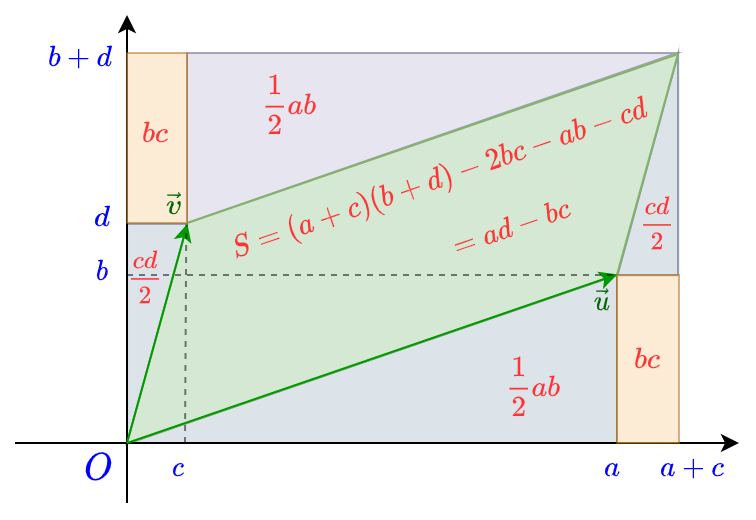
\includegraphics[scale=0.4]{paralel.png}
\end{center}

Теперь введем следующие переобозначения, чтобы связать площадь параллелогорамма с нашей основной темой главы. Положим
$$
\vec u = \vec u^{(1)} = (u^{(1)}_1,u^{(1)}_2), \quad \vec v = \vec u^{(2)} = (u^{(2)}_1,u^{(2)}_2).
$$

Тогда площадь $S$ параллелограмма вычисляется по формуле:
$$
S=\left|u^{(1)}_1u^{(2)}_2-u^{(1)}_2u^{(2)}_1\right|.
$$

\item Мы специально дали номера и векторам, и координатам, чтобы заметить одну особенность: первое произведение в этой формуле выбирает у первого вектора первую координату, а у второго вектора --- вторую. Во втором произведении номера векторов и координат перемешаны. Кроме того, данное выражение, если его взять без модуля, представляет собой определитель матрицы $2\times 2$. Определители матриц используются везде, где работает линейная алгебра --- от решения систем линейных уравнений и искусственного интеллекта до статистики и квантовой механики. В терминах определителя нахождение площди выглядит так:
\begin{center}
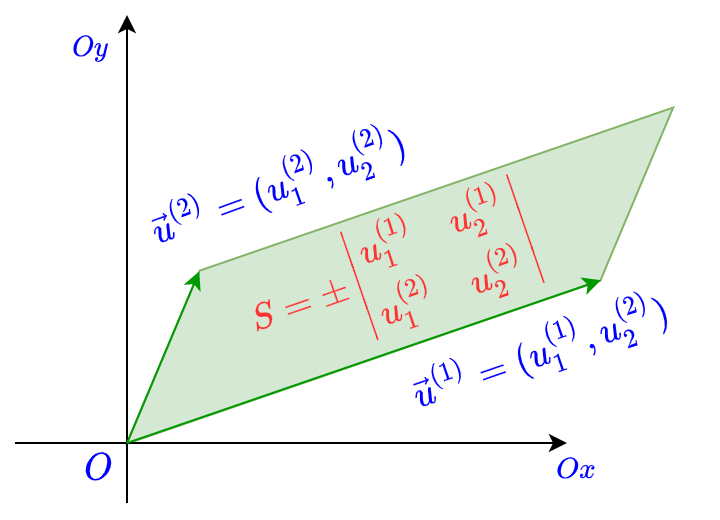
\includegraphics[scale=0.4]{paralel2.png}
\end{center}
Знак $\pm$ означает, что выбирается положительное итоговое значение, т.к. площадь не может быть отрицательной.
\item Но вернемся к перестановкам. Пусть номера векторов --- это элементы множества, на котором выполняется перестановка, а номера координат, выбранных у этих векторов, --- это перестановка номеров векторов. Тогда произведение $u^{(1)}_1u^{(2)}_2$ можно соотнести с тождественной перестановкой $\id=(1)(2)$, а произведение $u^{(1)}_2u^{(2)}_1$ --- с инверсной перестановкой $(12)$. Заметим также, что в случае переставленных номеров перед произведением появляется минус. В то же время, перестановка (12) является нечетной и ее знак тоже равен -1.
\item Аналогичным способом вычисляется объем $V$ параллелепипеда, построенного на трех векторах. Пусть даны три вектора в порстранстве:
$$
u^{(1)}=(u^{(1)}_1,u^{(1)}_2,u^{(1)}_3),\quad u^{(2)}=(u^{(2)}_1,u^{(2)}_2,u^{(2)}_3),\quad u^{(3)}=(u^{(3)}_1,u^{(3)}_2,u^{(3)}_3).
$$
Тогда объем $V$ равен модулю определителя координат трех векторов
$$
V=\pm\begin{vmatrix}
u^{(1)}_1 & u^{(1)}_2 & u^{(1)}_3 \\
u^{(2)}_1 & u^{(2)}_2 & u^{(2)}_3 \\
u^{(3)}_1 & u^{(3)}_2 & u^{(3)}_3 
\end{vmatrix},
$$
а определитель, в свою очередь, вычисляется следующим образом:
\begin{align*}
&
\begin{vmatrix}
u^{(1)}_1 & u^{(1)}_2 & u^{(1)}_3 \\
u^{(2)}_1 & u^{(2)}_2 & u^{(2)}_3 \\
u^{(3)}_1 & u^{(3)}_2 & u^{(3)}_3 
\end{vmatrix} = \sum_{\si\in\Sb_3} \sgn(\si) u^{(1)}_{\si(1)} u^{(2)}_{\si(2)} u^{(1)}_{\si(3)}= \\
& u^{(1)}_1 u^{(2)}_2 u^{(3)}_3 + u^{(1)}_2 u^{(2)}_3 u^{(3)}_1 +
u^{(1)}_3 u^{(2)}_1  u^{(3)}_2 - u^{(1)}_1 u^{(2)}_3  u^{(3)}_2 
 -u^{(1)}_3 u^{(2)}_2  u^{(3)}_1 -u^{(1)}_2 u^{(2)}_1 u^{(3)}_3,
\end{align*}
т.е. мы складываем трехкомпонентные произведения координат от каждого из векторов, используя все перестановки номеров и выставляя знак соответствующей перестановки.

Следующая графическая схема помогает запомнить правило вычисления определителя третьего порядка:
\begin{center}
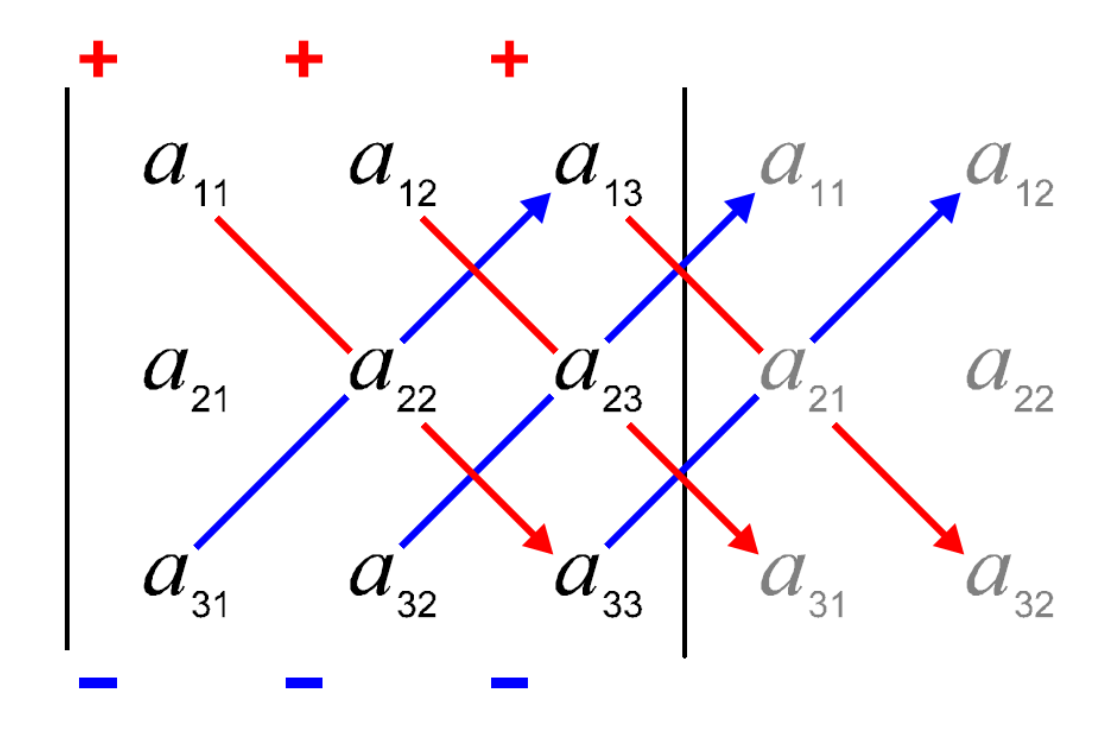
\includegraphics[scale=0.15]{Det.png}
\end{center}

\item На самом деле, и все определители более высокого порядка, и многомерные объемы вычисляются аналогичным способом.

\end{enumerate}










\begin{comment}
\chapter{10. Движения плоскости и пространства}
\end{comment}
\newchapter[и пространства]{Движения плоскости}

\vrezka{Данная глава продолжает тему групп движений. Здесь мы получаем теорему Шаля (для движений плоскости), а затем широкими мазками освещаем тему движений сферы и пространства. 

Разделы о сфере и пространстве могут быть пропущены при первом ознакомлении с текстом.
}

\section{Виды движений плоскости. Теорема Шаля}

\lesson{Байка про парад. Три вида движения плоскости. Связь с движениями окружности в случае неподвижной точки. Теоремы о неподвижных точках --- двух и трех}

\begin{enumerate}
\item \textbf{Иллюстративная сказка}. Представим себе Красную площадь и парад 9 мая. По площади идут ровные коробки участников парада. Чтобы не нарушать красоту и геометрию движения коробок, солдаты маршируют так, чтобы в каждый момент времени между любыми двумя из них сохранялось одно и то же расстояние. Иначе говоря, они осуществляют движение прямоугольной фигуры по плоскости площади. Затем точно так же делают колонны боевой техники.\index{Движения!плоскости}

По площади все они движутся равномерно и прямолинейно, пока им не придется осуществить поворот сначала на лобном месте на Васильевский спуск, а затем и на Кремлевскую набережную. И всякий поворот ради сохранения стройности шеренг и колонн нужно также осуществлять с сохраненим расстояний между всеми участниками парада. Таким образом движение плоскости можно иллюстрировать прямолинейным смещением и поворотом, а также их последовательными комбинациями.

Наконец, как и в случае окружности, возможно перестроение, при котором внутри одной коробки шеренги меняются ролями: первая шеренга становится последней, вторая --- предпоследней, и так далее. Здесь мы можем вспомнить аналогичную картинку с парковкой автомобилей, которую мы рассматривали ранее при описании движений прямой. Только вместо одного ряда машиномест у нас несколько шеренг. при перестроении они проходят в противоположных направлениях на равные расстояния относительно центральной шеренги. В итоге получается такая ж коробка, только стоявшие впереди участники оказываются сзади, и наоборот. И тут мы снова наблюдаем явление, при котором путаются направления --- вперед и назад. А если бы точно так же переместились колонны внутри коробки, то перепутались бы стороны --- правая и левая. Такое движение, переводящее коробку в себя и меняющее право-лево, либо перед-зад, называется осевой симметрией и оно также, как и в случае окружности, меняет пространственную ориентацию коробки.

\item Вернемся к геометрии.
Из приведенной иллюстрации понятно, что на плоскости существует как минимум три вида движений: параллельный перенос на некоторый вектор $v$, поворот на некоторый угол $\al$ относительно центра вращения в некоторо точке $O$ и симметрия относительно некоторой оси $l$. Первое мы обозначим $T_v$, второе --- $R^O_\al$, третье --- $S_l$. Параллельный перенос на вектор $v$ --- это такое движение, при котором все точки смещаются на вектор $v$ (т.е. в одном и том же направлении на одно и то же расстояние). Поворот --- это такое движение, при котором все точки сдвигаются по концентрическим окружностям на один и тот же угол в одном и том же направлении. Симметрия относительно оси $l$ --- это такое движение, при котором все точки плоскости переходят в симметричные относительно данной оси (т.е. из точки на ось $l$ опускается перпендикуляр, который затем продолжается на такое же расстояние, а все точки $l$ при этом остаются на месте).

\item Для движений плоскости, являющихся параллельным переносом, действует правило сложения параллелограмма. А именно, 
$$
T_v\circ T_u = T_{v+u},
$$
где сумма векторов $v+u$ осуществляется по правилу параллелограмма. Из этого же правила следует, что композиция параллельных переносов есть параллельный перенос, причем порядок слагаемых не имеет значения, т.е. параллельные переносы коммутируют друг с другом.

Для вращений существует аналогичное правило. если они имеют общий центр вращения:
$$
R^O_\al\circ R^O_\be = R^O_{\al+\be}.
$$
Ясно также, что в данном случае вращения коммутируют. т.к. они просто повторяют движения окружности с центром $O$.

Заметим также, что и параллельный перенос, и вращение, и осевая симметрия имеют обратные преобразования. Точнее, $T_v\circ T_{-v}=\id$, $R^O_\al\circ R^O_{-\al}=\id$, а также $S_l\circ S_l=\id$. То есть, эти движения обратимы. Отсюда же следует, что они являются биекциями.

Для вывода остальных свойств арифметики движений нам потребуются некоторые дополнительные сведения о движениях плоскости.

\item Для начала мы рассмотрим случай, когда движение плоскости сохраняет на месте хотя бы одну точку. Назовем такое движение буквой $G$. Выберем какую-нибудь неподвижную точку  движения $G$ и обозначим ее за $O$. Теперь возьмем любую окружность с центром $O$  обозначим ее $S^1$. Что происходит с ней при таком движении? Ясно, что она переходит в себя, поскольку движение сохраняет расстояние, а все точки окружности равноудалеын от центра $O$.

Но тогда получается, что движение $G$ порождает движение окружности $S^1$. Покажем, что разные движения плоскости порождают разные движения окружности. Пусть движения плоскости $G_1$ и $G_2$ оставляют на месте точку $O$, но при этом не равны, т.е. как минимум одна точка $A$ на плоскости переходит в первом случае в $A_1$, а во втором --- в $A_2$, причем $A_1\ne A_2$.

Здесь мы обратимся к одному из важнейших методов геометрии: \textit{проецированию}. А конкретно, --- к проецированию точки на окружность. Соединим точку $O$ с точкой $A$ и, в случае необходимости, продолжим отрезок до пересечения его с окружностью $S^1$ так, чтобы точки $A$ и $A'$ (точка пересечения) лежали по одну сторону от центра $O$. Аналогично построим точки $A_1'$ и $A_2'$.

Далее заметим, что если бы $A_1'=A_2'$, то, очевидно, $A_1$ и $A_2$ оказались бы на одной прямой, причем по одну сторону от $O$. Но в силу свойств движения, т.е. равенства расстояний $|OA_1|=|OA|=|OA_2|$, оказалось бы также, что $A_1=A_2$, что противоречит предположению.

Итак, разные движения плоскости, сохраняющие точку $O$, порождают и разные движения окружности $S^1$ с центром $O$.

Обратно, всякому движению окружности соответствует движение плоскости. Действительно, как мы знаем, движение окружности есть либо вращение, либо симметрия относительно оси, проходящей через центр $O$. В таком случае, возьмем в качестве движения $G$ плоскости либо вращение относительно центра $O$ на тот же угол, либо симметрию относительно той же оси.

Сказанное выше означает, что \textit{все движения плоскости, имеющие общую неподвижную точку $O$, взаимно однозначно определяются одноименными движениями окружности с центром в той же точке $O$}. Говоря алгебраическим языком, множество движений плоскости содержит в себе группы, изоморфные группе движений окружности. Этих групп столько, сколько точек на плоскости.

Чтобы доказать, что все движения плоскости образуют группу, нам потребуется описать все виды движений и построить их таблицу умножения.

\item Редуцирование движений плоскости с неподвижной точкой к движениям окружности, сразу же дает нам возможность понять, что такие движения бывают всего двух видов: повороты (в том числе $\id$) и осевые симметрии. Причем, первый случай получается тогда, когда у движения есть ровно одна неподвижная точка, либо вся плоскость неподвижна. А симмметрия окружности предполагает неподвижность двух диаметриально противоположных точек. Ясно, что при этом не только эти две точки $S^1$ останутся неподвижными.
\begin{lem} Если движение плоскости сохраняет неподвижными две различные точки, то оно сохраняет неподвижными все точки прямой, проходящей через данные две точки.
\end{lem}
\pf Пусть движение $G$ плоскости оставляет на месте точки $A\ne B$. Для начала заметим, что движение $G$ в этом случае прямую $AB$ переводит в саму себя. Действительно, если бы это было не так, то три различные точки $A,B,C$, лежащие на этой прямой, перешли бы в треугольник $ABC'$, где $C'=G(C)$. Но тогда нарушается неравенство треугольника, при котором сумма двух сторон всегда больше третьей, а для трех точек на одной прямой это не так.

Следовательно, $G$ порождает движение прямой $AB$. Но для движения прямой нам уже хорошо известно, что если движение сохраняет на месте две точки на месте, то оно сохраняет все точки этой прямой на месте!
\epf

\item Наконец, остается тривиальный вариант для случая неподвижных точек у движения плоскости.
\begin{thrm}\index{Теорема!о трех гвоздях}
Если движение $G$ плоскости оставляет на месте три точки, не лежащие на одной прямой, то $G=\id$.
\end{thrm}
\pf
Пусть даны три точки $A,B,C$, не лежащие на одной прямой, такие, что $G(A)=A$, $G(B)=B$ и $G(C)=C$. Возьмем окружность $S^1$ с центром в точке $A$. Движение $G$ порождает на этой окружности либо поворот, либо симметрию. Построим проекции точек $B$ и $C$ на данную окружность, получим точки $B'$ и $C'$.

Из доказанной выше леммы следует, что движение $G$ сохраняет на месте прямые $AB$ и $AC$. Эти прямые различны, т.к. иначе бы точки $ABC$ оказались на одной прямой. Следовательно, $A'\ne B'$. В то же время, это точки прямых $AB$ и $AC$, а значит, они являются стационарными точками движения $G$. 

Итак, мы имеем движение окружности, которое сохраняет на месте две различные точки, не являющиеся диаметрально противоположными. А про такое движение мы уже знаем, что является $\id$, т.е. поворотом на нулевой угол. Стало быть, таковым же является и $G$.
\epf

\item Движение плоскости различные точки переводит в различные. Действительно, если бы это было не так, и мы бы имели $G(A)=G(B)$, хотя $A\ne B$, то, взяв произвольную точку $C$, отличную от $A$ и $B$, мы бы получили, что движение $G$ переводит треугольник в отрезок $G(A)G(C)$, что приводит к нарушению неравенства треугольника. Итак, движение плоскости является инъекцией.


\lesson{Движения плоскости: Нет неподвижных точек. Композиция не более трех симметрий. Скользящая симметрия. Теорема Шаля}

\item Посмотрим, что происходит, когда у движения $G$ нет неподвижных точек. Возьмем произвольную точку $O$ и обозначим $A=G(O)$. По предположению $A\ne O$. В таком случае, мы можем построить серединный перпендикуляр отрезка $AO$, который мы обозначим за $l$, и рассмотреть симметрию $S_l$ плоскости относительно него. Тогда, очевидно, композиция движений $S_l\circ G$ сохраняет на месте точку $O$, и мы оказываемся в описанных выше условиях.

Это значит, что движение $S_l\circ G$ является либо поворотом $R^O_\al$ с центром в точке $O$ на угол $\al$, либо симметрией $S_m$ относительно прямой $m$, проходящей через точку $O$. Но тогда, применяя слева симметрию $S_l$, находим, что
$$
G=S_l\circ R^O_\al,\mbox{ либо }G=S_l\circ S_m.
$$

В свою очередь, поворот $R^O_\al$, если его рассматривать как движение окружности $S^1$ с центром $O$, как мы ранее выяснили, является композицией двух симметрий относительно осей $n,k$, угол между которыми равен $\al/2$. Таким образом,
$$
G=S_l\circ S_n\circ S_k,\mbox{ либо }G=S_l\circ S_m.
$$

\item Итак, в том случае, когда движение не сохраняет на месте ни одной точки, оно является композицией двух или трех симметрий.
\begin{thrm}
Всякое движение плоскости есть композиция не более чем трех осевых симметрий.
\end{thrm}
\item Отсюда, в частности, следует, что всякое движение плоскости биективно.

\item Выше мы дали обозначения трем видам движений плоскости: параллельный перенос, поворот и осевая симметрия. Возникает вопрос: исчерпываются ли движения плоскости только такими движениями или есть какие-то еще?

\item Пусть снова движение $G$ таково, что оно не сохраняет на месте ни одной точки. Возьмем произвольную точку $A$ и далее обозначим $B=G(A)$, $C=G(B)$. Поскольку $G$ --- движение (изометрия), $AB=BC$. Если $C$ лежит на прямой $AB$, то вся прямая $A$ под действием движения $G$ пеереходит в себя (иначе бы нарушалось неравенство треугольника), причем точки располагаются в порядке $A<B<C$ (иначе бы мы получили $A=C$, и тогда середина отрезка $AB$ будет стационарной точкой $G$).

Предположим далее, что $C$ не лежит на прямой $AB$. В этом случае обозначим за $X$ середину $AB$, за $Y$ --- середину $BC$, и через точки $X,Y$ проведем прямую $L$. Необходимо показать, что $L$ переходит в себя под действием $G$.

\begin{center}
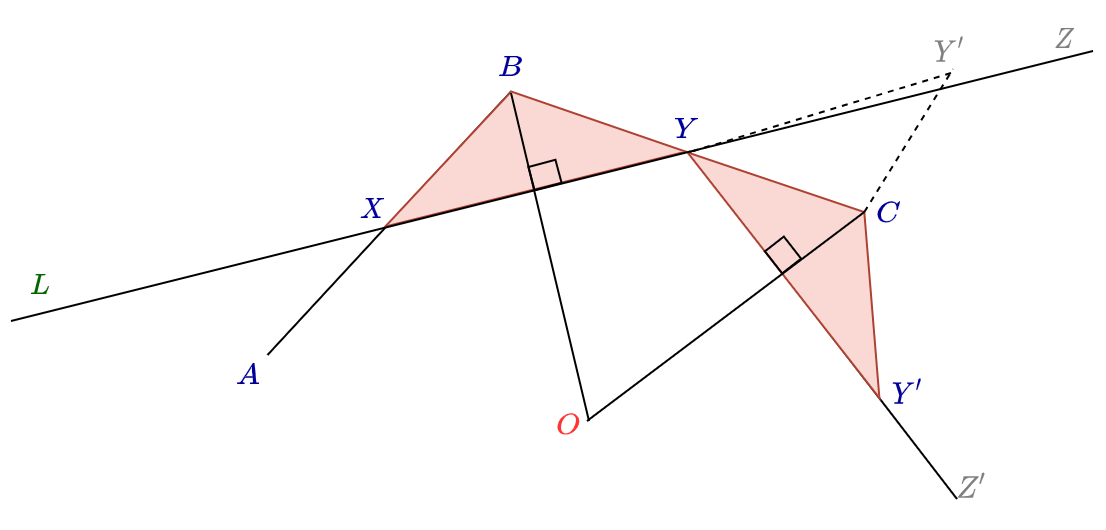
\includegraphics[scale=0.3]{Skolz.png}
\end{center}


Пусть $Y'=G(Y)$. Ясно, что $XY=YY'$, причем $X\ne Y'$, иначе бы середина $XY$ оказалсь стационарной точкой $G$. Точки $X$ и $Y'$ могут лежать по одну или по разные стороны прямой $BC$. Если они лежат по разные стороны, от рассмотрим треугольники $\triangle XYB$ и $\triangle YY'C$. Они равны по трем сторонам в силу того, что $G$ является движением, кроме того, они оба равнобедренные с основаниями $XY$ и $YY'$, соответственно. Но тогда равны углы $\angle XYB=\angle Y'YC$ при вершине $Y$, отложенные в разные стороны прямой $BC$, т.е. эти углы являются вертикальными, откуда следует, что точка $Y'$ находится на прямой $L$. Мы снова получаем ситуацию трех точек в порядке $X<Y<Y'$, откуда следует, что вся прямая $L$ переходит в себя под действием $G$.

Наконец, предположим, что $X$ и $Y'$ оказались по одну сторону прямой $BC$. В этом случае мы можем построить серединные перпендикуляры отрезков $XY$ и $YY'$, которые пересекутся в некторой точке $O$. Пусть $O'=G(O)$. Треугольник $XOY$ равнобедренный, он переходит под действием $G$ в треугольник $YO'Y'$, также равнобедренный. Это значит, что точка $O'$ лежит на серединном перпендикуляре отрезка $YY'$, причем на таком же расстоянии от середины $YY'$, как и точка $O$ от середины  $XY$. Но отрезок $BO$ пересекает отрезок $XY$. Значит, в силу свойств движения, отрезок $CO$ пересекает отрезок $YY'$. И тогда для точки $O'$ остается единственная возможность: $O=O'$. А это противоречит тому, что $G$ не имеет стационарных точек.

Итак, предположение о том, что $G$ не имеет неподвижных точек, приводит к тому, что найдется прямая $L$, которая под действием $G$ переходит в себя. Это значит, что $G$ действует на $L$ как смещение (отражение имело бы неподвижную точку, а других движений на прямой не существует).

Смещение на $L$ задается вектором $XY$ (или $AB$, если мы остались в первом варианте). Составим композицию $G\circ T_{-XY}$. Очевидно, что такое движение плоскости оставляет на месте прямую $L$. Как мы уже выяснили, это соответствует либо $\id$, либо осевой симметрии $S_L$. Таким образом, $G=T_{XY}$, либо $G=S_L\circ T_{XY}$, причем вектор $XY$ параллелен прямой $L$.

\item Итак, движение $G$, которое не сохраняет на месте ни одной точки, является либо параллельным переносом, либо симметрией с последующим параллельным переносом вдоль оси симметрии на ненулевой вектор. Во втором случае движение $G$ называется \textbf{скользящей симметрией}.

\item Легко понять, что скользящая симметрия не сводится к другим видам движений, если ее смещение не нулевое. Действительно, $\id$, поворот и осевая симметрия исключаются из-за наличия неподвижных точек. Параллельный перенос исключается, поскольку при нем отрезок $AG(A)$ не может пересекать никакую прямую, параллельную сдвигу.

\item Скользящую симметрию с осью симметрии $l$ и параллельным переносом вдоль этой оси на вектор $u$ будем обозначать $T_uS_l$ (без значка композиции). Для ее обозначения часто используют символ $W_u$, не указывая явно ось симметрии, т.к. вектор $u$ однозначно ее задает. Но в случае $u=0$ это не так, и поэтому для надежности мы будем использовать два индекса, понимая, что вектор $u$ параллелен оси $l$.

\item Окончательно получаем
\begin{thrm}[Шаля] Всякое движение плоскости (без разложения его на компоненты) есть движение одного из следующих классов:\index{Теорема!Шаля}
\begin{enumerate}[a)]
\item класс параллельных переносов (на произвольный вектор, в том числе нулевой), который мы обозначим $\rightrightarrows$;
\item класс поворотов относительно произвольного центра, который мы обозначим $\circlearrowleft$;
\item класс \textbf{скользящих симметрий} (осевая симметрия с последующим сдвигом на произвольный вектор, параллельный оси симметрии), который мы обозначим $\leftharpoonup\leftharpoondown$.
\end{enumerate}
\end{thrm}
Обычную симметрию относительно неподвижной оси мы теперь отнесем также в класс скользящих симметрий как частный случай при нулевом сдвиге. Точно так же, как относим $\id$ к классу параллельных переносов и поворотов.


\lesson{Построение полной таблицы композиций движений плоскости: переносы и повороты}

\item Таблица композиций для таких классов выглядит следующим образом:\index{Таблица композиций}
\begin{center}
\begin{tabular}{c|ccc}
 & $\rightrightarrows$ & $\circlearrowleft$ &  $\leftharpoonup\leftharpoondown$ \\ \hline
$\rightrightarrows$ & $\rightrightarrows$ &  $\circlearrowleft$ &  $\leftharpoonup\leftharpoondown$  \\ 
$\circlearrowleft$ & $\circlearrowleft$ & $\rightrightarrows$ или $\circlearrowleft$ & $\leftharpoonup\leftharpoondown$  \\ 
$\leftharpoonup\leftharpoondown$ & $\leftharpoonup\leftharpoondown$ & $\leftharpoonup\leftharpoondown$ & $\rightrightarrows$ или $\circlearrowleft$  \\ 
\end{tabular}
\end{center}

Наша дальнейшая задача --- обосновать данную таблицу, построив полную таблицу композиций движений плоскости.

\item Итак, нам нужно найти все попарные комбинации композиций переноса, поворота и скользящей симметрии, причем мы выделим отдельно частный ее случай --- симметрию.

\item Ясно, что $T_u\circ T_v=T_{u+v}$, причем данная композиция коммутативна.

\item Рассмотрим композицию $T_v\circ R_\al^O$. Из свойств движений окружности мы знаем, что поворот можно представить как композицию двух симметрий , а из свойств движений прямой --- что сдвиг тоже можно представить как композицию двух симметрий. Пусть $R_\al^O=S_2\circ S_1$ и $T_v=S_4\circ S_3$. При этом оси симметрий $1$ и $2$ пересекаются в точке $O$, а угол между ними равен $\al/2$ и откладывается от оси 1 к оси 2. Оси 3 и 4 параллельны друг другу и перпендикулярны направлению сдвига, причем расстояние между ними равно $v/2$, а направление сдвига --- от оси 3 к оси 4.

Заметим, что выбор осей 1 и 2 произволен в рамках требований общей точки пересечени и угла между осями. Сама пара осей может быть повернута как угодно, в частности, можно выбрать ось 2 так, чтобы она оказалась перпендикулярной вектору сдвига $v$. Кроме того, выбор осей 3 и 4 также произволен в рамках требований расстояния между ними и строго перпендикулярного положения к вектору сдвига. Саму пару осей можно двигать вдоль вектора $v$ как угодно. Поэтому совместим ось 3 с осью 2.

Имеем следующее:
$$
T_v\circ R_\al^O = (S_4\circ S_3)\circ (S_2\circ S_1) = S_4\circ (S_3\circ S_2)\circ S_1 = S_4\circ S_1,
$$
где мы сократили $S_3\circ S_2$, т.к. это одна и та же симметрия. Полученная композиция $S_4\circ S_1$ является поворотом на тот же угол $\al$, только с новым центром $O_1$, который получем как пересечение осей 1 и 4.
\begin{center}
\includegraphics[scale=0.2]{plane_transit.png}
\end{center}

Аналогично поступаем в случае композиции $R_\be^A\circ T_u$ (см. рисунок). При этом новый центр поворота смещается на вектор $-u/2$ и перпендикулярно ему на величину $|u/2|/\tan(\be/2)$. Видим также, что композиция сдвига и поворота не коммутативна (кроме случая, когда перенос осуществляется на нулевой вектор).

\item Рассмотрим композицию двух поворотов $R_\be^A\circ R_\al^O$. Снова представим кажджый поворот как композицию симметрий, и снова, пользуясь произвольностью наклона пары осей симметрий, расположим их так, чтобы вторая ось первого поворота и первая ось второго поворота совпали с прямой $OA$ (см. рисунок). Если углы таковы, что их сумма не равна нулю, то 1 и 4 оси пересекутся, и точка $C$ их пересечения окажется центром результирующего поворота. А угол поворота станет равным $\al+\be$.

Если же $\al+\be=0$, то оси 1 и 4 будут параллельны, и композиция поворотов превратится в паралельный перенос на расстояние $2AO\sin(\al/2)$.

Заметим также, что два поворота будут коммутировать тогда и только тогда, когда $\al=\be$, т.к. только в этом случае точка $C$ будет одна и та же при различном порядке композиции.


\lesson{Таблица композиций движений плоскости: отражения и скользящая симметрия}

\item Рассмотрим композицию $G=T_{\vec v}\circ S_l$. Чтобы понять, что это такое, воспользуемся тем же приемом, с помощью которого мы показали наличие еще одного вида движений плоскости --- скользящей симметрии. Именно, возьмем на прямой $l$ точку $A$ и проследим за ее судьбой при двух итерациях преобразования $G$. Получатся точки $B$ и $C$. Далее, через точки $X$ и $Y$, являющиеся серединами отрезков $AB$ и $BC$, проведем прямую $m$. Эта прямая при преобразовании $G$ переходит сама в себя. Все остальные точки сначала отражаются относительно $m$, затем смещаются в направлении вектора $\vec{AC}$, но на половину его длины. Обозначим $\vec w=\vec{AB}$. Тогда получим, что $G=T_{\vec w}\circ S_m$.

\begin{center}
\includegraphics[scale=0.3]{slides.png}
\end{center}

Условимся записывать $\vec w=\Pr_l\vec v$, что означает проекцию вектора $\vec v$ на ось $l$, а также $m=l+\vec v/2$, что означает сдвиг оси $l$ в направлении $\vec v$ на половину его длины. Тогда получим, что
$$
T_{\vec v}\circ S_l = T_{\Pr_l\vec v}\circ S_{l+\vec v/2},
$$
а это не что иное, как скользящая симметрия.

В симметричном случае получим
$$
S_l\circ T_{\vec u} = T_{\Pr_l\vec u}\circ S_{l-\vec u/2},
$$
т.е. тоже скользащая симметрия с тем же сдвигом, но с симметричной относительно $l$ осью симметрии.

Все сказанное справедливо, если угол наклона $l$ не прямой и не нулевой относительно вектора $\vec v$. Если окажется, что $l\perp\vec v$, то $G=S_{l+\vec v/2}$, поскольку смещение $\Pr_l\vec v=0$. Если же $l\parallel\vec v$, то исходное преобразование $G$ уже есть скользаящая симметрия с осью $l$ и смещением $\vec v$. Эти случаи вписываются в общую формулу, если иметь ввиду, что $l+\vec v/2=l$ в том случае, когда $l\parallel\vec v$.

\item Рассмотрим композицию $G=R_\be^A\circ S_l$. В качестве отправной точки $A_1$ возьмем точку, симметричную центру вращения $A$ относительно $l$. Тогда $A_1$ переходит в $A=B$, а далее $B$ переходит в $C$ (см. рисунок). Снова проводим среднюю линию $XY$ в полученном равнобедренном треугольнике. Тогда вектор $\vec w = \vec{XY}$ есть смещение новой скользящей симметрии, а ось $m$, полученная вращением оси $l$ вокруг точки $X$ на угол $\be/2$ --- осью скользящей симметрии.
$$
R_\be^A\circ S_l = T_{\vec w}\circ S_m,\quad \vec w  = 2 \Pr_m\vec{XA},\quad X = \Pr_lA.
$$
Заметим, что в том случае, когда $A\in l$, получаем $\vec w=0$, и композиция $G$ становится просто симметрией $S_m$.

В симметричном случае получим
$$
S_m\circ R_\al^O = T_{-\vec w}\circ S_k,\quad \vec w  = 2 \Pr_k\vec{XO},\quad X = \Pr_mO.
$$

Для внесения данных в итоговую таблицу обозначим за $l+\be/2$ ось $m$, полученную из оси $l$ поворотом на угол $\be/2$ относительно точки $X$ --- проекции центра вращения $A$ на ось $l$. Аналогично, $m-\al/2$. Тогда
$$
R_\be^A\circ S_l = T_w\circ S_{l+\be/2},\quad S_m\circ R_\al^O = T_{-w}\circ S_{m-\al/2}.
$$

\item Композиция двух симметрий $S_m\circ S_l$, как и в случае окружности, есть поворот $R_{2\angle lm}^{l\cap m}$, где $\angle lm$ есть угол от оси $l$ до оси $m$, а центр вращения есть общая точка этих осей. Если угол между осями равен нулю, и при этом они не совпадают, а просто параллельны друг другу, то, как мы уже знаем, их композиция есть параллельный перенос в направлении от $l$ к $m$ (перпендикулярно им) на удвоенное расстояние между осями симметрии. Такой перенос обозначим $T_{2(m-l)}$.

\item Осталось рассмотреть композиции со скользящей симметрией. Пусть $G=T_v\circ T_uS_l$. Очевидно, что это на самом деле композиция $T_{u+v}\circ S_l$, и мы приходим к уже рассмотренному случаю композиции переноса и симметрии. Обратно, если $G$ есть композиция $T_vS_m\circ T_u$, то поскольку в скользящей симметрии перенос и симметрия коммутируют, запишем $G$ как
$S_m\circ T_{v+u}$, и мы снова имеем дело с изученной ситуацией.

\item Пусть далее $G=R_\be^A\circ T_uS_l$. В таком случае
$$
G = (R_\be^A\circ T_u)\circ S_l = R_\be^{A_1}\circ S_l,
$$
т.е. снова приходим к изветсному случаю с заменой лишь центра вращения. В симметричном случае $T_vS_m\circ R_\al^O$ все аналогично.

\item Наконец, пусть $G=S_m\circ T_uS_l$. Здесь можно пойти разными путями для получения результата. Проще выглядит путь, при котором мы сначала найдем композицию двух симметрий:
$$
G = (S_m\circ S_l)\circ T_u = \begin{cases} R_{2\angle ml}^O, & l\not\parallel m, \\
T_{2(m-l)+u}, & l\parallel m,\end{cases}
$$
в первом случае центр симметрии $O$ зависит от вектора $u$.

Аналогично,
$$
T_vS_m\circ S_l = T_v\circ(S_m\circ S_l) = \begin{cases} R_{2\angle ml}^O, & l\not\parallel m, \\
T_{2(m-l)+v}, & l\parallel m,\end{cases}
$$
где центр симметрии $O$ зависит от вектора $v$.

\item Осталось рассмотреть случай композиции двух скользящих симметрий:
$$
T_vS_m\circ T_uS_l = T_v\circ(S_m\circ S_l)\circ T_u =\begin{cases} R_{2\angle ml}^O, & l\not\parallel m, \\
T_{2(m-l)+u+v}, & l\parallel m,\end{cases}
$$
где центр симметрии $O$ зависит уже от обоих переносов $u$ и $v$.

\item Сведем все полученные результаты в таблицу.\index{Группа!движений плоскости}

\renewcommand{\arraystretch}{1.8}\renewcommand{\tabcolsep}{1mm}
\begin{center}\tiny
\begin{tabular}{c|c|c|c|c|}
$\id$  &  $T_u$      &   $R_\al^O$   &   $S_l$   & $T_uS_l$  \\
\hline
$T_u$  &  $T_{u+v}$  &   $R_\al^{O_1}$ & $T_{\Pr_lv}S_{l+v/2}$ & $T_{\Pr_l[u+v]}S_{l+(u+v)/2}$ \\ \hline 
$R_\be^A$ & $R_\be^{A_1}$ & \specialcell{$R_{\al+\be}^C$ ($\al+\be\ne 0$) \\ $T_w$ ($\al+\be=0$)} & \specialcell{$T_wS_{l+\be/2}$ ($A\notin l$) \\ $S_{l+\be/2}$ ($A\in l$)} & \specialcell{$T_wS_{l+\be/2}$ ($A_1\notin l$) \\ $S_{l+\be/2}$ ($A_1\in l$)} \\ \hline 
$S_m$ & $T_{\Pr_lu}S_{m-u/2} $ & \specialcell{$T_wS_{m-\al/2}$ ($O\notin m$) \\ $S_{m-\al/2}$ ($O\in m$)} &
\specialcell{$R_{2\angle lm}^{l\cap m}$ ($l\not\parallel m$) \\ $T_{2(m-l)}$ ($l\parallel m$)} & 
\specialcell{$R_{2\angle lm}^O$ ($l\not\parallel m$) \\ $T_{2(m-l)+u}$ ($l\parallel m$)} \\ \hline 
$T_vS_m$ & $T_{\Pr_l[u+v]}S_{m-(u+v)/2}$ & \specialcell{$T_wS_{m-\al/2}$ ($O_1\notin m$) \\ $S_{m-\al/2}$ ($O_1\in m$)} &
\specialcell{$R_{2\angle lm}^O$ ($l\not\parallel m$) \\ $T_{2(m-l)+v}$ ($l\parallel m$)} &
\specialcell{$R_{2\angle lm}^O$ ($l\not\parallel m$) \\ $T_{2(m-l)+u+v}$ ($l\parallel m$)} \\ \hline
\end{tabular}
\end{center}

\end{enumerate}


\subsection*{Задачи}
\begin{enumerate}
\item Найти композицию отражения относительно вертикальной оси и поворота на $180^o$ относительно точки, не лежащей на оси симметрии.
\item Пусть дан произвольный треугольник. На его сторонах построим правильные треугольники и соединим их центры. Доказать, что полученный треуголник --- правильный.
\end{enumerate}


\section{Сравнение движений прямой, окружности и плоскости}


\lesson{Общие слова о схожести движенией прямой и окружности, окружности и плоскости. Понятие ориентации}

\begin{enumerate}
\item Отметим несколько общих свойств рассмотренных нами движений прямой, окружности и плоскости.
\item Во-первых, их всех можно свести к композиции симметрий. Для одномерных объектов (прямая и окружность) --- не более двух, для двумерных --- не более трех.
\item Во-вторых, все движения можно разделить на два класса: сохраняющие и меняющие \textbf{ориентацию}. Те движения, которые сводятся к композиции четного числа симметрий, сохраняют ориентацию фигур, а те, которые сводятся к композиции нечетного числа симметрий, --- меняют ориентацию фигур. Изменение ориентации означает, что право и лево меняются местами, т.е. мы как бы переходим в зазеркалье. 
\item При этом нужно отметить, что преобразования, меняющие ориентацию, обязательно требуют выхода в пространство более высокой размерности (для прямой --- в плоскость, а для окружности и плоскости --- в пространство размерности 3), если мы хотим осуществить их непрерывным движением.
\item В-третьих, есть и более глубинная связь движений прямой, окружности и плоскости. Мы уже отмечали, что окружность можно рассматривать как прямую, у которой склеили противоположные концы (где-то на бесконечности). И с этой точки зрения сдвиг на прямой является прямой аналогией вращения окружности. Особенно, если величина сдвига сильно меньше радиуса.
\item А симметрия прямой при этом естественным образом превращается в симметрию окружности. Только ось симметрии должна проходить через место склейки двух бесконечностей. Остальные же симметрии можно получить дополнительным сдвигом, т.е. вращением.
\item Далее, окружность находится на плоскости. И поэтому вращение окружности полностью аналогично вращению плоскости, если при этом совместить их центры.
\item Еще проще увидеть совпадения понятий сдвига на прямой и плоскости. В обоих случаях мы просто смещаем все точки на какой-то вектор.
\item Тем не менее, на плоскости появляется новый вид движения, который комбинирует в себе сдвиг и отражение относительно оси сдвига. Это --- скользаящая симметрия, т.е. симметрия с последующим применением сдвига вдоль оси симметрии. На одномерных объектах такое движение в принципе невозможно. На прямой симметрия относительно этой же прямой ничего не дает, т.е. является $\id$, а на окружности симметрия относительно самой окружности вообще требует специального построения в геометрии плоскости.
\end{enumerate}



\section{Пара слов о движениях сферы}


\lesson{Движения сферы: вращения, отражения, зеркальные вращения (аналог скользящей симметрии). Теорема Шаля}

\begin{enumerate}\index{Движения!сферы}
\item Имея опыт перехода от прямой к окружности, мы можем легко найти движения сферы, отправляясь от движений плоскости.
\item Представим себе сферу как плоскость, у которой бесконечно удаленный край был стянут в точку (метод <<хинкали>>).
\item Во что превращаются при этом движения плоскости?
\item Сдвиг, он же параллельный перенос, превращается в такое движение, при котором все точки движутся по параллельным траекториям. С точки зрения географии это есть движение вдоль широтных линий. Да, проходят они при этом разное расстояние! Из-за чего, кстати, и появляются силы Кориолиса, создающие океанические течения вроде Гольфстрима. Но собственные расстояния между точками сохраняются, и это, несомненно, движение.
\item Вращение, которое, как мы помним, на окружности соответствует сдвигу на прямой, в случае сферы в прямом смысле слова совпадает со сдвигом! Дело в том, что вращение сферы вокруг оси, --- это вращение вокруг полюса, при котором угол поворота измеряется меридианом. Но ведь то же самое движение около экватора есть то, что мы только что отнесли к сдвигам вдоль широтных линий.
\item Таким образом, сдвиг прямой и вращение окружности в случае сферы чудесным образом объединяются в один вид движений --- осевое вращение. И это делает движения сферы чуть проще, чем движения плоскости, где сдвиг можно представить лишь как композицию двух вращений.
\item Далее, симметрия плоскости относительно прямой естественным образом переходит в отражение сферы относительно центральной секущей плоскости или, иначе говоря, относительно окружности большого круга. При такой симметрии полюса сферы меняются местами (полюса определются пересечением со сферой прямой, пересекающей плоскость отражения в центре сферы и перпендикулярной ей), а плоскость отражения остается на месте.
\item Наконец, скользящая симметрия плоскости есть композиция сдвига и осевой симметрии, и ей на сфере соответствует \textbf{зеркальное вращение}, т.е. композиция отражения и вращения параллельно плоскости отражения.
\item Таким образом, все движения сферы распадаются на два класса: вращения и зеркальные вращения. При этом, все движения есть композиция не более чем трех отражений.
\item Этот аналог теоремы Шаля для сферы можно доказать, используя очередную лемму о гвоздях, предполагая неподвижность пары противоположых точек (случай одной точки на плоскости), неподвижность целой окружности большого круга (случай двух точек на плоскости), отсутствие неподвижных точек.
\end{enumerate}

\subsection*{Задачи}
\begin{enumerate}
\item Построить таблицу движений сферы аналогично таблице движений плоскости (символику придумайте сами).
\item **Доказать, что других движений на сфере не существует (лемма о гвоздях).
\end{enumerate}


\section{Пара слов о движениях пространства}



\lesson{Движения пространства: винт (в частности, сдвиг, осевое вращение, $\id$), зеркальное вращение (в частности, отражение), скользящая симметрия (в частности, отражение). Итоговая таблица классов собственных и несобственных движений прямой, окружности, плоскости, сферы и пространства}

\begin{enumerate}\index{Движения!пространства}
\item Наконец, мы можем от сферы перейти к пространству. На самом деле, переход в пространство сопровождается лишь добавлением сдвига в пространстве. Т.е. любое движение сферы можно рассматривать как движение пространства с одной неподвижной точкой --- центром сферы. После чего можно применить сдвиг этого центра, и получить новые движения. Понятно, что никаких других движений тут быть не может.
\item Тем не менее, классификация движений пространства становится сложнее примерно так же, как классификация движений плоскости превосходит классификацию движений окружности. А именно, в пространстве появляется \textbf{винтовое движение} как композиция осевого вращения и сдвига вдоль оси вращения. Это --- обобщение скользящей симметрии на плоскости (если винт осуществляет поворот на $180^0$, мы как раз получаем скользящую симметрию).
\item Есть также и собственно \textbf{скользящая симметрия пространства}. Это --- отражение относительно плоскости с последующим сдвигом вдоль направления, параллельного данной плоскости. Такое движение также является обобщением скользящей симметрии на плоскости.
\item Заметим, что более сложное движение винт включает в себя более простые. Так, если винт имеет нулевой сдвиг, то он доставляет осевое вращение, а если винт имеет нулевой поворот, то он доставляет сдвиг. Понятно, что в случае полного зануления параметров винта мы получим $\id$.
\item Точно так же, \textbf{зеркальное вращение}, как и в случае сферы, при нулевом повороте доставляет просто симметрию.
\item Наконец, скользящая симметрия своим частным случаем имеет просто симметрию относительно плоскости.
\item Таким образом, классификация движений пространства включает следующие виды движений:
\begin{enumerate}[a)]
\item винт (в частности, сдвиг, осевое вращение, $\id$);
\item зеркальное вращение (в частности, отражение);
\item скользящая симметрия (в частности, отражение).
\end{enumerate}
\end{enumerate}

\subsection*{Задачи}
\begin{enumerate}
\item Построить таблицу движений пространства аналогично таблице движений плоскости (символику придумайте сами).
\item *Показать, что центральная симметрия пространства --- это зеркальное вращение.
\item **Доказать, что других движений в пространстве не существует (лемма о гвоздях).
\end{enumerate}


\begin{sidewaystable}
\caption{Сравнение движений.}
\label{Transitions}
\begin{tabular}{p{2cm}|p{2.5cm}p{2.5cm}p{2.5cm}p{2cm}p{2.5cm}p{2.5cm}}
\rowcolor{darkred}
& \multicolumn{3}{P{8.5cm}}{\textcolor{white}{\bfseries Собственные движения\linebreak (не меняют ориентацию)}} & \multicolumn{3}{P{8cm}}{\textcolor{white}{\bfseries Несобственные движения\linebreak (меняют ориентацию)}} \\ 
& Перенос & Поворот & Смещение поворота & Симметрия & \multicolumn{2}{p{5cm}}{Смещенная симметрия} \\ \hline \hline
Прямая     & сдвиг на число & & & относи\-тель\-но точки & & \\  \hline
Окруж\-ность & \multicolumn{2}{p{5cm}}{\centerline{вращение}} & & осевая симметрия & & \\ \hline
Плос\-кость  & параллель\-ный перенос & относи\-тель\-но точки & & осевая симметрия & скользящая симметрия (перенос+ сим\-мет\-рия) & \\  \hline
Сфера & вращение вблизи экватора & вращение вблизи полюса & & отражение относительно плоскости & \multicolumn{2}{p{5cm}}{зеркальное вращение (вращение+симметрия)} \\ \hline
Прост\-ранство & параллель\-ный перенос & осевое вращение & винт (перенос + вращение) & отражение относительно плоскости & скользящая симметрия (перенос+ сим\-мет\-рия) & зеркальное вращение (вращение+ сим\-мет\-рия) \\ \hline \hline
\end{tabular}
\end{sidewaystable}




\begin{comment}
\chapter{11. Комплексная арифметика и алгебра}
\end{comment}
\newchapter[и алгебра]{Комплексная арифметика}

\vrezka{
В этой главы мы начинаем строить поле комплексных чисел, пока еще без участия вещественных. По сути мы здесь работаем только с комплексными рациональностями, что, однако, не мешает показать тесную геометрическую связь комплексных чисел и движений плоскости, а также изучить числа Гаусса.
}


\section{Алгебра комплексных чисел}

\lesson{Комплексные числа, мотивация: $x^2+1=0$, алгебраизация плоскости. Сложение, умножение, сопряжение, модуль, обратное число}

\begin{enumerate}
\item Когда мы строили поле $\Q[\sqrt 2]$, мы ввели в обращение новое число, которое позволяло решать уравнение $x^2=2$. Это число не является рациональным, но лежит где-то между рациональными числами. Тогда же мы задались вопросом, как быть с поиском корней других уравнений с целыми коэффициентами, неразрешимых в $\Q$.
\item Рассмотрим еще один пример уравнения: $x^2=-1$.
\item Ворде бы, все коэффициенты --- целые числа, и степень всего лишь вторая. Однако же, при детальном рассмотрении становится ясно, что у него нет решений не только в рациональных числах, но и где-то между ними, поскольку никакое известное нам число, возведенное в квадрат, и близко не подходит к -1.
\item Стало быть, если мы хотим ввести в обращение корень такого уравнения, то его наобходимо поместить где-то вне числовой оси, <<подвесить в воздухе>>.
\item Сделаем это из чисто эстетико-геометрических соображений. Как геометрически проявляют себя числа на прямой? Они обеспечивают сдвиг вдоль прямой: положительные --- вправо, отрицательные --- влево. Причем у всех этих сдвигов есть единица измерения --- число 1, которая заодно выступает и в роли мультипликативной единицы, когда мы определяем умножение чисел. Кроме того, сдвиг на 1 вправо и затем влево (или в обратном порядке) приводит нас обратно, т.е. является сдвигом на 0, или $\id$.
\item Новое же число мы хотим поместить так, чтобы оно обеспечивало сдвиг на плоскости, аналогичный сдвигу вдоль прямой.
\item Поскольку мы привыкли считать направление <<вверх>> положительным, поместим это число над числовой осью.
\item Заложим в этом числе сразу и единицу измерения: пусть оно отстоит от нуля на расстояние 1, тем самым мы согласуем масштаб сдвигов на плоскости со сдвигами на прямой. Наконец, сдвиг в направлении и на величину этой новой единицы не должен содержать в себе горизонтальных сдвигов, их проще добавить потом, взяв от сдвигов прямой, которые нам уже известны. Иначе говоря, числовая прямая при сдвиге на эту новую единицу должна сдвиуться вверх на расстояние 1 и таким образом, чтобы ее числовая разметка никуда не сдвинулась вправо или влево.
\item Так мы приходим к тому, что новую единицу сдвига следует отложить от нуля строго вверх на расстояние 1.
\item На координатной сетке она окажется в точке $(0,1)$.
\item Назовем это новое число-вектор буквой $i$,  которую принято называть \textbf{мнимой единицей} (от фр. \textit{imaginaire}).\index{Мнимая единица}
\item Теперь всякий сдвиг плоскости мы можем записать как композицию сдвига, выраженного в единицах (горизонтальный сдвиг), и сдвига, выраженного в мнимых единицах (вертикальный сдвиг). Просто по свойствам суммы векторов.
\item Иначе говоря, сдвиг на произвольный вектор $\vec z$ мы распишем как сдвиг на сумму векторов $x\vec 1+y\vec i$. См. рис.
\begin{center}
\includegraphics[scale=0.5]{complex.png}
\end{center}
\item Как и прежде, мы умеем отличать на плоскости векторы и точки. Векторы --- это направленные отрезки, которые можно откладывать от точек. Сложение векторов означает их последоватеьлное откладывание. В результате таких откладываний мы уходим от некоторой стартовой точки и приходим в какую-то финишную точку. Результирующий вектор соединяет стартовую и финишную точки. Договоримся для удобства считать стартовой точкой начало координат $O$, а финишную точку обозначать почти так же, как вектор, который в нее входит, только без векторной символики.
\item Итак, если вектор равен $x\vec 1+y\vec i$, то его финишная точка обозначается $x+yi$.
\item Пока все, что мы сделали --- это построили обычную арифметику векторов на плоскости. При чем же тут алгебраическая ипостась мнимой единицы, вытекающая из уравнения $x^2=-1$?
\item Алгебраическая ипостась $i$ нам нужна как раз для того, чтобы построить алгебру точек плоскости, т.е. научиться их не только складывать и умножать на число, но еще и умножать и делить друг на друга.
\item Примем за аксиому, что с числами вида $x+iy$ мы будем обращаться как с обычными числами, пользуясь аксиомами поля, и при этом пользоваться тем самым свойством мнимой единицы, которое ее определяет, т.е. равенством $i^2=1$.
\item Например,
$$
(a+bi)(x+yi) = ax + ayi + bxi + byi^2 = (ax-by) + (ay+bx)i.
$$
\item Числа вида $z=x+iy$ с заданными операциями сложения и умножения (сложение --- покоординатное, а умножение определено выше) называются \textbf{компл\'eксными числами}.\index{Числа!компл\'eксные} При этом $x$ называется \textbf{действительной} (или вещественной) частью комплексного числа $z$ и имеет также обозначение $\Re z$, а $y$ называется \textbf{мнимой} частью числа $z$ и имеет также обозначение $\Im z$.
\item Координатная ось $Ox$ на комплексной плоскости называется действительной осью, а координатная ось $Oy$ --- мнимой.
\item Дадим следующие определения. Число $\bar z=x-yi$ называется \textbf{комплексно сопряженным} к числу $z=x+iy$. Комплексное сопряжение --- это отражение относитеьлно действительной оси.
\item Модулем комплексного числа $z=x+yi$ называется число $$|z|=\sqrt{x^2+y^2}.$$
Нетрудно видеть, что модуль комплексного числа --- это длина соответствующего ему вектора (по теореме Пифагора). Кроме того, из геометрических соображений понятно, что $|z_1-z_2|$ --- это расстояние между точками $z_1$ и $z_2$ на плоскости.
\begin{center}
\includegraphics[scale=0.5]{rho.png}
\end{center}
\item Посмотрим, какие арифметические свойства комплексных чисел можно извлечь.
\begin{enumerate}[\bf C1)]
\item $z\bar z=|z|^2$. Действительно, $(x+yi)(x-yi)=x^2+y^2$.
\item $z=0$ (т.е. $z=0+0i$) тогда и только тогда, когда $|z|=0$.
\item Обратное по умножению число для $z\ne 0$ существует и равно
$$
z^{-1} = \frac{1}{x+yi}=\frac{x-yi}{(x+yi)(x-yi)}=\frac{\bar z}{|z|^2}
$$
Это можно получить и напрямую из свойства C1.
\item Мультипликативное свойство сопряжения: $\bar{zw}=\bar{z}\,\bar{w}$. Действительно,
$$ 
\bar{(x+yi)(a+bi)} = \bar{(ax-by)+(ay+bx)i} = (ax-by)-(ay+bx)i
$$
и
$$
\bar{(x+yi)}\,\bar{(a+bi)} = (x-yi)(a-bi) = (ax-by)-(ay+bx)i.
$$
\item Мультипликаивное свойство модуля: $|zw|=|z||w|$. Действительно,
$$
|zw|^2 = zw\bar{zw} = zw\bar{z}\,\bar{w} = z\bar{z}w\bar{w} = |z|^2|w|^2.
$$
\end{enumerate}


\lesson{Сложение как параллельный перенос. Умножение на единичное число как поворот. Аргумент комплексного числа. Сопряжение как симметрия относительно вещественной оси}


\item Сложение с числом $z=x+iy$ --- это параллельный перенос $T_{\vec z}$ на вектор $\vec z=x\vec 1+y\vec i$. Это следует из геометрических свойств комплексных чисел, о которых мы говорили выше.

Кроме того, это легко проверить арифметически. Пусть даны две точки $z_1$ и $z_2$. Добавим к ним вектор $z$, получим новые точки $z_1'=z_1+z$ и $z_2'=z_2+z$. Во-первых, заметим, что расстояние сохранилось:
$$
|z_1'-z_2'| = |(z_1+z)-(z_2+z)| = |z_1-z_2|,
$$
т.е прибавление $z$ --- это движение. Во-вторых, если $z\ne 0$, то у этого движения нет неподвижных точек, иначе мы бы получили равенство $z_1+z=z_1$, откуда $z=0$. Следовательно, в силу теоремы Шаля прибавление $z$ есть параллельный перенос. Прибавление $z=0$ есть $\id$.

\item Умножение на комплексное число, по модулю равное 1, есть поворот с центром в нуле.

Пусть $|z|=1$. Возьмем точки $w_1=a_1+b_1i$ и $w_2=a_2+b_2i$,  умножим их на $z$, получим точки $w_1'=w_1z$ и $w_2'=w_2z$.

Найдем расстояние между $w_1'$ и $w_1'$:
$$
|w_1'-w_2'|=|(w_1-w_2)z|=|w_1-w_2|\cdot|z|=|w_1-w_2|,
$$
т.е. умножение на $z$ сохраняет расстояние. В то же время, очевидно, что при $z\ne 1$ единственной неподвижной точкой при умножении будет $w=0$, иначе мы бы получили $wz=w$, т.е. $z=w/w=1$. Умножение на $z=1$ есть $\id$.

Итак, умножение на число $z$, по модулю равное 1, является поворотом с центром в нуле. \textit{Каков при этом угол поворота?} 

Чтобы ответить на данный вопрос, рассморим для начала случай $|w|=1$, т.е. точку с единичой окружности будем умножать на другую точку с единичной окружности. По свойствам модуля имеем $|zw|=|z||w|=1$, т.е. в результате умножения мы вновь получим точку на единичной окружности! Иначе говоря, единичная окружность с операцией умножения комплексных чисел образует группу.

Теперь, заметим, что на окружности радиуса 1 хорда однозначно определяет опирающийся на нее угол. Рассмотрим углы, которые опираются на хорду $[z;1]$ и на хорду $[zw;w]$. На рисунке они выделены красным цветом.
\begin{center}
\includegraphics[scale=0.4]{complex-ring.png}
\end{center}

Легко видеть, что длины хорд равны: $|zw-w|=|z-1||w|=|z-1|$, так что и углы равны. Следовательно, точка $zw$ получается из точки $w$ поворотом на угол, соответствующий угу наклона вектора $z$ относительно положительного направления действитеьлной оси.

Что происходит в случае, когда $w$ не лежит на единичной окружности и отлична от нуля? Для этого представим произведение $zw$ следующим образом:
$$
zw = z\frac{w}{|w|}|w|,
$$
где отношение $w/|w|$ уже является комплексным числом единичной длины. Следовательно, число $zw/|w|$ получается из числа $w/|w|$ его поворотом на угол, заданный числом $z$. Осталось выяснить, как связаны $w$ с $w/|w|$ и $zw$ с $zw/|w|$.

В общем случае это означает, что мы имеем два комплексных числа, одно $v$, второе $\la v$, где действительное число $\la>0$. Пусть $v=a+bi$. Вспомним уравнение прямой, проходящей через начало координат и точку $(a,b)$. Это уравнение имеет вид $ay-bx=0$. А теперь умножим в этом уравнении обе части на $\la$, и получим $(\la a)y-(\la b)x=0$. То есть точка $\la v$ лежит на той же прямой, что и $v$.

Остался вопрос --- с одной ли стороны относительно нуля они лежат? Чтобы это проверить, нужно сравнить длину их разности с суммой длин:
$$
|\la v-v|=|v||\la-1|<(1+\la)|v|=|v|+|\la v|,
$$
т.е. да, они лежат на одной прямой по одну сторону от нуля.
\begin{center}
\includegraphics[scale=0.4]{complex-ring2.png}
\end{center}

Итак, число $zw$ получается следующим способом: сначала $w$ переводится на единичную окружность нормировкой, т.е. делением на модуль, получается $w/|w|$. Затем оно поворачивается на угол, заданный числом $z$, затем оно возвращается на свою орбиту, т.е. домножается на $|w|$. В итоге это есть не что иное, как поворот точки $w$ на угол, заданный числом $z$.
\item Кстати, угол, заданный числом $z$, а в общем случае, числом $z/|z|$ (если $z$ --- произвольное ненулевое комплексное число), называется \textbf{аргументом числа} $z$ и обозначается $\arg z$.
\item Основные тригонометрические функции определяются с помощью комплексного числа с единичной окружности так: пусть задан угол $\ph$. Повернем вектор $(1,0)$ на этот угол и найдем число $z$ на единичной окружности такое, что $\arg z=\ph$, тогда
$$
\cos\ph = \Re z,\quad \sin\ph=\Im z.
$$
\item Как уже отмечалось выше, операция комплексного сопряжения есть не что иное как отражение относительно действительной оси. Так что все базовые виды движений плоскости у нас представлены. Учитывая также, что поворот с произвольным центром можно представить как композицию сдвига, поворота с центром в нуле и обратного сдвига, а отражение относительно произвольной оси --- как композицию поворота или сдвига, отражения относительно действитеьлной оси и обратного поворота или сдвига, приходим к тому, что все движения плоскости можно выразить через три изученных нами действия с комплексными числами: сложение (произвольный сдвиг), умножение на число с единичной окружности (поворот с центром в нуле) и сопряжение (отражение относительно действитеьлной оси).
\item На будущее у нас остается вопрос: \textit{какое преобразование плоскости осуществляет умножение на произвольное ненулевое комплексное число?}
\item Поскольку мы пока знакомы только с рациональными дробями, комплексные числа у нас также являются рациональными, т.е. имеют вид $\frac{a}{b}+\frac{c}{d}i$, где $a,b,c,d\in\Z$ и $b,d\ne 0$. Но даже при таком существенном ограничении мы уже имеем дело с еще одним полем --- \textbf{полем комплексных рациональностей},\index{Поле!комплексных рациональностей} поскольку сложение, вычитание, умножение и деление не выводит нас за пределы этого множества (единственное исключение --- модуль числа может выпасть из $\Q$). Такое поле обоначается $\Q[i]$ и является расширением поля $\Q$, аналогично полю $\Q[\sqrt 2]$, рассмотренному ранее.
\end{enumerate}

\subsection*{Задачи}

\begin{enumerate}
\item Докажите, что если $\la>0$, то $|\la-1|<\la+1$.
\item Вычислить, нарисовать на плоскости и указать модуль и аргумент следующих комплексных чисел:
$$
i^2,\;i^3,\;i^4,\;1/i,\;(1+2i)(2-i),\;(1+i)(1+2i)(1+3i),\;\frac{1}{1+i},\;\frac{5}{2-i}.
$$
\end{enumerate}


\section{Гауссовы целые числа}

\lesson{Делимость гауссовых чисел. Норма. Группа корней 4 степени из 1. Ассоциированные числа. Свойства делимости}
\index{Гауссовы целые числа}\index{Числа!гауссовы}\index{Кольцо!гауссовых целых чисел}

\begin{enumerate}
\item В этом разделе мы ограничимся рассмотрением комплесных чисел с целыми координатами, т.е. чисел вида
$$
a+bi,\quad a,b\in\Z
$$
Легко видеть, что такие числа образуют коммутативное кольцо с единицей. Данное кольцо обозначается $\Z[i]$ и называется кольцом \textbf{гауссовых целых чисел}. На координатной плоскости точки $\Z[i]$ сосредоточены в узлах целочисленной решетки.
\item Число $a+bi$ \textbf{делится на} $c+di$, если существует число $a'+b'i$ такое, что $a+bi=(c+di)(a'+b'i)$. Обозначение аналогично обычному в натуральных числах: $(c+di)|(a+bi)$. Например, число 2 делится на $(1+i)$, т.\,к. $2=(1+i)(1-i)$.\index{Делимость чисел}

\item 
Нормой гауссова числа $a+bi$ называется величина $$N(a+bi)=(a+bi)(a-bi)=a^2+b^2,$$
т.е. норма числа $z$ равна $z\bar z$

 Несколько свойств нормы:
\begin{enumerate}[{\bf Norm1}]
\item $N(a+bi)=0$ тогда и только тогда, когда $a=b=0$.
\item Нормы комплексно сопряженных чисел совпадают.
\item Если норма нечётна, то она имеет вид $4k+1$, никакая норма не может быть равна $4n+3$.

Поскольку $N(a+bi)=a^2+b^2$, легко видеть, что она является нечетным числом только в том случае, когда $a$ четное, $b$ нечетное, либо наоборот. Пусть $a=2k$, $b=2j+1$, тогда $a^2+b^2=4k^2+4j^2+4j+1 = 1\pmod 4$.

\item $N(zw)=N(z)N(w)$, где $z,w$ --- гауссовы числа.

Пусть $z=a+bi$, $w=c+di$, тогда
\begin{align*}
N(zw)    & = N(ac-bd+i(ad+bc)) = a^2c^2+b^2d^2+a^2d^2+b^2c^2 \\
N(z)N(w) & = (a^2+b^2)(c^2+d^2) = a^2c^2+a^2d^2+b^2c^2+b^2d^2.
\end{align*}
\end{enumerate}
Последнее свойство означает, что  делителями единицы (обратимыми элементами) могут быть только числа с нормой 1, т.\,е. $\pm 1$ и $\pm i$. Других обратимых нет. Геометрически делителями единицы, являются те и только те гауссовы числа, которые лежат на единичной окружности. Отметим также, что все делители единицы образуют множество всех корней 4 степени из 1, т.е. корней уравнения $x^4=1$.

Наконец, множество $\{1,-1,i,-i\}$ является группой по умножению, причем уже хорошо знакомой нам группой, если не обращать внимание на символ операции и символы элементов группы. Сравните таблицы <<умножения двух групп>>: этой и группы сложения вычетов по модулю 4 $\Z_4$:
\begin{center}
\begin{tabular}{c||c|c|c|c|}
* & 1 & i & -1 & -i\\
\hline\hline
1 & 1 & i & -1 & -i\\ \hline
i & i & -1 & -i & 1 \\ \hline
-1 & -1 & -i & 1 & i \\ \hline
-i & -i & 1 & i & -1 \\ \hline
\end{tabular}
\qquad
\begin{tabular}{c||c|c|c|c|}
$+$ &0 & 1 & 2 & 3\\
\hline\hline
0 &0 & 1 & 2 & 3\\ \hline
1 &1 & 2 & 3 & 0 \\ \hline
2 &2 & 3 & 0 & 1 \\ \hline
3 &3 & 0 & 1 & 2\\ \hline
\end{tabular}
\end{center}

Если произвести соответствие $1\mapsto 0$, $i\mapsto 1$, $-1\mapsto 2$, $-i\mapsto 3$, а операции умножения поставить в соответствие операцию сложения по модулю 4, то мы получим и полное соответствие между результатами умножения в первой группе и сложения во второй: $i(-1)\mapsto 1+2$ и т.д.

В том случае, когда можно предъявить взаимно однозначное соответствие элементов двух групп так, чтобы операция в первой группе соответствовала операции во второй, говорят о том, что эти две группы \textbf{изоморфны}. Очень часто такие группы даже считают равными, хотя природа у них разная. Итак, группа по умножению обратимых гауссовых чисел изоморфна группе $\Z_4$.\index{Изоморфизм групп}


\item Все гауссовы числа делятся на делители единицы. Это легко понять из групповых свойств делителей единицы. Действительно, разделить на 1 означает умножить на нее, т.к. 1 сама себе обратна по умножению. Разделить на $i$ означает умножить на $-i$, т.к. эти числа взаимно обратны по умножени. Аналогично, разделить на $-1$ означает умножить на -1, и разделить на $-i$ означает умножить на $i$.

\item Делители единицы обладают еще одним замечательным свойством: умножение на них --- это поворот относительно начала координат, причем умножение на $i$ есть поворот на угол $\pi/2$, умножение на -1 --- поворот на угол $\pi$ (т.е. центральная симметрия), умножение на $-i$ --- поворот на угол $3\pi/2$ или $-\pi/2$. То есть делители единицы соответствуют еще и группе вращений квадрата.


\item Два гауссовых числа называют \textbf{ассоциированными},\index{Числа!ассоциированные гауссовы} если одно получается из другого умножением на делитель единицы. Ассоциированность является отношением эквивалентности, причем каждый класс эквивалентности включает ровно 4 числа, расположенных в углах квадрата с центром в 0. Например, $1+2i$, $-2+i$, $-1-2i$ и $2-i$ ассоциированы.
\begin{center}
\includegraphics[scale=0.35]{Gaussian.png}
\end{center}

\item Свойства делимости гауссовых чисел очень похожи на таковые свойства в арифметике натуральных чисел, но есть и отличия.
Приведем несколько свойств:
\begin{enumerate}[\bf\hbox{Div}1]
\item Если гауссово число $a+bi$ делится на обычное целое число $c+i0$, то $c|a$ и $c|b$ в целых числах.

Это легко видеть из равенства $a+bi=(x+yi)(c+i0)=xc+yci$, откуда $a=xc$ и $b=yc$.
\item Если $z|w$ и $w|z$, то $z$ и $w$ ассоциированы.

Пусть $w=z'z$ и $z=w'w$, откуда $N(w)=N(z')N(z)$ и $N(z)=N(w')N(w)$, откуда $N(z')N(w')=1$ и, следовательно, $N(z')=N(w')=1$, поскольку в натуральных числах это единственное решение. Стало быть, $z'$ и $w'$ --- делители единицы.

\item Ассоциированность сохраняет делимость: если $z$ и $w$ ассоциированы, $u$ и $v$ ассоциированы, то $(z|u)\to (w|v)$.

Действительно, пусть $z=z'w$ и $u=u'v$, где $z',u'$ --- делители единицы. Тогда
$$
\frac{u}{z} = \frac{u'}{z'}\frac{v}{w},
$$
так что если отношение $u/z$ является гауссовым числом, то отношение $v/w$ является ассоциированным с ним числом.
\item $z$ ($N(z)>1$) имеет как минимум 8 делителей: своих ассоциированных и ассоциированных с 1.
\item Делители $z$ являются делителями $N(z)$, если $N(z)$ рассматривать как гауссово число.

Пусть $w|z$, т.е. $z=uw$. Поскольку $N(z)=z\bar z=w(u\bar z)$, очевидно, что $N(z)$ делится на $w$.
\item Норма $z=a+bi$ четна тогда и только тогда, когда $(1+i)|z$, в частности, если $a$ и $b$ имеют разную четность, то $z$ не делится на $1+i$.

Для начала заметим, что норма $z=a+bi$ четна тогда и только тогда, когда $a$ и $b$ имеют одинаковую четность, т.е. сравнимы по модулю 2. Далее, поскольку $(1+i)|z$, существует $c+di$ такое, что
$$
a+bi = (1+i)(c+di) = c-d + i(c+d),
$$
т.е. $a=c-d$, $b=c+d$, что равносильно $a-b=-2d$, $a+b=2c$ при некоторых $с,d\in\Z$, а это равносильно тому, что $a\equiv b\pmod 2$.
\end{enumerate}


\lesson{Деление гауссовых чисел с остатком, алгоритм Евклида, представление НОД в виде линейной комбинации}


\item В кольце $\Z[i]$ можно любое число $u$ разделить на любое число $v\ne 0$ с остатком, так что получится
\begin{equation}\label{Ostat}
u=qv+r,\quad N(r)<N(v).
\end{equation}
При этом выбор чисел $q$ и $r$ можно строго ограничить, выбирая $q$ как ближайшее гауссово число к комплексному $u/v\in\Q[i]$, а $r$ как разность между $u$ и $qv$. В случае, когда выбор $q$ неоднозначен (может быть максимум 4 числа), можно договориться выбирать то, которое на координатной сетке находится левее и/или ниже.

Приведем один из вариантов вычисления $r$. Пусть $u=a+bi$ и $v=c+di$. Далее оперируем в поле $\Q[i]$:
$$
\frac{a+bi}{c+di}=\frac{(ac+bd)+(bc-ad)i}{c^2+d^2}=q_1+\frac{r_1}{c^2+d^2}+q_2i+\frac{r_2}{c^2+d^2}i,
$$
где $ac+bd=q_1(c^2+d^2)+r_1$ и $bc-ad=q_2(c^2+d^2)+r_2$. Здесь мы воспользовались делением с остатком в кольце $\Z$. При этом мы выбираем знаки $r_1$ и $r_2$ так, чтобы выполнялись неравенства:
$$
|r_1|,|r_2|\le (c^2+d^2)/2.
$$
Это всегда возможно, поскольку остатки от деления можно выбирать не только из ряда $0,1,2,\dots,c^2+d^2-1$, но также из ряда
$0,\pm 1,\pm 2,\dots,\pm k$, где $k$ --- целая часть от деления $c^2+d^2$ на 2, так что всегда $k\le(c^2+d^2)/2$. Здесь как раз и может оказаться вплоть до 4-х вариантов выбора.

Тогда
$$
u=(q_1+q_2i)v+\frac{(r_1+r_2i)(c+di)}{c^2+d^2}=(r_1+r_2i)\frac{v}{N(v)},
$$
эту последнюю дробь мы и выберем в качестве остатка $r$.

При этом заметим, что поскольку разность $u-(q_1+q_2i)v$ является гауссовым числом, то таковым же будет и число $(r_1/N(v)+r_2i/N(v))v$, хоть оно и выглядит нецелым.

Далее,
$$
N\left(\frac{r_1}{N(v)}+\frac{r_2}{N(v)}i\right)=\frac{r_1^2+r_2^2}{(c^2+d^2)^2}\le \frac 12,
$$
откуда $N(r)\le (1/2)N(v)<N(v)$.

\item На основе деления с остатком нетрудно получить выполнимость алгоритма Евклида (см. раздел \ref{EVKL}) для гауссовых чисел:
\begin{align*}
u & = q_1v + r_1, &  N(r_1)<N(v),\\
v & = q_2r_1 + r_2, &  N(r_2)<N(r_1),\\
r_1 & = q_3r_2 + r_3, &  N(r_3)<N(r_2),\\
\dots & \dots & \\
r_{n-1} & = q_{n+1}r_n + r_{n+1}, &  N(r_{n+1})<N(r_n),\\
r_{n} & = q_{n+2}r_{n+1}, &  N(r_{n+1})<N(r_n),\\
\end{align*}
поскольку норма является натуралным числом и не может убывать бесконечно.

Отсюда так же, как для целых чисел, выводится и представление $\gcd(u,v)$ в виде линейной комбинации исходных чисел $u,v$. Но мы докажем этот факт иным способом.
\begin{lem}\label{NOD}
Для любых гауссовых чисел $u,v\ne 0$ существует гауссово число $r$ такое, что:

\textup{1)} $r|u$ и $r|v$ (общий делитель);

\textup{2)} если $(q|u)\wedge(q|v)$, то $q|r$ (наибольший общий делитель);

\textup{3)} существуют гауссовы $x,y$ такие, что $r=xu+yv$.

\noindent Кроме того,

\textup{4)} число $r$, удовлетворяющее \textup{1)--3)}, единственное с точностью до ассоциированности.
\end{lem}
\pf
Рассмотрим множество $R(u,v)=\{xu+yv|\;x,y\in\Z[i]\}\setminus\{0\}$. В множестве норм $\{N(z)|\;z\in R(u,v)\}$ существует наименьшее положительное число (т.\,к. нуля там быть не может). Пусть $r\in R(u,v)$ такое число, у которого норма минимальная (оно может быть не единственное, выберем одно). Остается показать, что $r$ --- искомое.

Во-первых, $r$ имеет вид $xu+yv$ по построению, т.е. выполняется пункт 3). Во-вторых, если $(q|u)$ и $(q|v)$, то очевидно, что $q|r$ также по построению $r$, т.е. выполняется пункт 2).

Докажем пункт 1).
Из \eqref{Ostat} имеем: $u=rt+s$, где $N(s)<N(r)$. Подставляя представление $r$, имеем:
$u=xut+yvt+s$, откуда $s=(1-xt)u+(-yt)v$. Если $s\ne 0$, то $s\in R$ как линейная комбинация $u$ и $v$, но тогда $N(s)\ge N(r)$ в силу выбора $r$, а это не так в силу \eqref{Ostat}. Следовательно, $s=0$, откуда $r|u$. Аналогично, $r|v$.

Докажем пункт 4). Пусть $r'=x'u+y'v$ также удовлетворяет свойствам 1)--3). Тогда $r|r'$ и $r'|r$. Из первого следует, что $r'=rt$ и $N(r')=N(r)N(t)$, из второго следует, что $r=r't'$ и $N(r)=N(r')N(t')$. Таким образом, нормы $N(t)$ и $N(t')$ взаимно обратны в натуральных числах, откуда следует $N(t)=N(t')=1$, т.\,е. $t$ --- делитель 1 и, следовательно, $r$ и $r'$ ассоциированы.
\epf

\item Доказанная лемма позволяет определить понятие НОД для гауссовых чисел с точностью до ассоциированности. В качестве НОД мы будем выбирать какое-то одно из четырех (наиболее удобного вида).



\lesson{Гауссовы простые числа. Рождественская теорема Ферма. Критерий Гаусса. ОТА гауссовых чисел}

\item Гауссово число называется \textbf{простым}, если оно не имеет никаких делителей, кроме тривиальных (ассоциированных с 1 и самим собой), и не является делителем 1, т.\,е. простое гауссово число имеет ровно 8 делителей. Два гауссовых числа называются \textbf{взаимно простыми} (обозначается $u\perp v$), если их НОД --- обратимое число, т.\,е. 1 и ассоциированные с ней.

\item Верны следующие свойства простых гауссовых чисел:
\begin{enumerate}[\bf\hbox{Prim}1]
\item Если $a+bi$ простое, то $a-bi$ также простое.

Действательно, если $a-bi=uv$, где $u,v$ не ассоциированы с 1, то $a+bi=\bar u\bar v$, где $\bar u$ и $\bar v$ не ассоциированы  с 1 (т.к. для делителей нуля сопряжение не нарушает ассоциированности), нотогда $a+bi$ не является простым.
\item Если $z$ простое, то его ассоциированные также простые.
\item Если $z$ простое и $z|uv$, то $(z|u)\vee(z|v)$;

Действительно. Пусть простое $z|uv$. Предположим, что $\neg(z|u)$, тогда $z\perp u$, откуда по лемме \ref{NOD} получаем, что $1=xz+yu$. Умножаем на $v$: $v=xzv+yuv$. Справа оба слагаемых делятся на $z$, следовательно, $z|v$. Аналогично, если $\neg(z|v)$, то $z|u$.

\item Норма простого, неассоциированного с $1+i$, всегда нечетна, т.\,е. имеет вид $4k+1$.

Это следует из свойства Div6. Если простое число не ассоциировано с $1+i$, то оно и не делится на него, а значит, по свойству Div6 его норма нечетная. То, что она имеет вид $4k+1$, следут из $(2k)^2+(2n+1)^2=4m+1$.
\item Натуральное простое не всегда есть гауссово простое: $5=(2+i)(2-i)$.
\item Простое натуральное $4k+1$ можно представить как сумму квадратов $a^2+b^2$ (\textbf{рождественская теорема Ферма}).\index{Теорема!рождественская теорема Ферма}
\pf Рассмотрим факториал $(p-1)!$ в арифметике по модулю $p$. Поскольку $-1\equiv p-1$, $-2\equiv p-2$ и т.д., а всего множителей $p-1=4k$, то все они разбиваются на пары вида $1,-1$, $2,-2$, и т.д., $(p-1)/2,-(p-1)/2$, откуда
\begin{multline*}
(p-1)! \equiv 1(-1)2(-2)\dots\frac{p-1}{2}\frac{-p+1}{2} \equiv \\
 (-1)^{(p-1)/2}\left(\frac{p-1}{2}!\right)^2 \equiv \left(\frac{p-1}{2}!\right)^2\pmod p,
\end{multline*}
поскольку $(p-1)/2=2k$ --- четное число. С другой стороны, по теореме Вильсона \ref{Wilson} $(p-1)!\equiv p-1\pmod p$, так что
$$
p-1\equiv \left(\frac{p-1}{2}!\right)^2\pmod p,
$$
то есть, $p-1$ сравнимо с квадратом некоторого числа $c$, откуда следует, что $c^2+1$ делится на $p$.

Теперь переходим в числа Гаусса: $c^2+1=(c+i)(c-i)$. Если число $p$ --- простое в гауссовых числах, то в силу ОТА либо $c+i$ делится на $p$, либо $c-i$ делится на $p$, тогда по свойству Div1 число $1$ делится на $p$, что невозможно. Следовательно, $p$ --- не простое гауссово число, а значит,
$$
p = (a+bi)(x+yi),
$$
где оба множителя нетривиальны. В то же время $p$ --- не комплексное число, т.е. $p=\bar p$, т.е.
$$
p = (a-bi)(x-yi),
$$
наконец, норма $p$ будет равна
$$
p\bar p=p^2=(a^2+b^2)(x^2+y^2).
$$

А теперь возвращаемся в обычные натуральные числа, поскольку слева и справа именно они. Число $p$ --- простое, стало быть, его квадрат в силу ОТА раскладывается единственным образом на произведение $p$ и $p$, откуда
$$
p=(a^2+b^2)=(x^2+y^2),
$$
что и завершает доказательство.
\epf

\item Рождественская теорема Ферма еще проще выводится из критерия Гаусса того, что комплексное число является простым гауссовым числом. Доказательство этого критерия мы оставим за рамками курса.
\begin{thrm}[Критерий Гаусса]
$a+bi$ простое тогда и только тогда, когда\\
\textup{1)} либо одно из чисел $a,b$ нулевое, а второе --- простое целое число вида $\pm(4k+3)$ ($k>0$), \\
\textup{2)} либо $a,b$ ненулевые и норма $N(a+bi)=a^2+b^2$ --- простое натуральное число.
\end{thrm}
\item \textbf{Следствие}: простое натуральное вида $4k+1$ не может быть простым гауссовым, простые натуральные вида $4k+3$ являются простыми гауссовыми.

\item Из данного следствия рождественская теорема Ферма следует в один шаг (см. конец доказательства, приведенного выше).

\item Если $N(z)\perp N(w)$ в натуральных числах, то $z\perp w$ в гауссовых числах.

Пусть $u=\gcd(z,w)$ в гауссовых числах. Тогда $z=ut$, $w=ut'$ и $N(z)=N(u)N(t)$, $N(w)=N(u)N(t')$. Откуда $N(u)|N(z)$ и $N(u)|N(w)$. Тогда из условия $N(z)\perp N(w)$ следует, что $N(u)=1$, т.\,е. $u$ --- ассоциированное с 1 гауссово число. Откуда $z\perp w$.
\end{enumerate}
Примеры простых гауссовых чисел: $\pm 3, \pm 7, \pm 3i$; $1\pm i, 1\pm 2i, 1\pm 4i$.

\item Для гауссовых чисел существует аналог основной теоремы арифметики (см. раздел \ref{PrimeNumbers}):\index{Теорема!ОТА гауссовых чисел}
\begin{thrm}[Основная теорема арифметики гауссовых чисел]\label{OTAG}\quad\\
Каждое ненулевое неассоциированное с 1 гауссово число раскладывается на гауссовы простые множители, причем это разложение единственно с точностью до ассоциированных с этими множителями простых и порядка множителей, т.\,е. разложение имеет вид
$$
\al_1^{s_1}\dots \al_n^{s_n}=\be_1^{s_1}\dots \be_n^{s_n},
$$
где пары $\al_i,\be_i$ являются ассоциированными простыми числами, а степени $s_i$ --- натуральными числами.
\end{thrm}
Доказательство теоремы прямо следует из свойства Prim3.

Пример: $5=(2+i)(2-i)=(1+2i)(1-2i)$ (множители переводятся друг в друга умножением на $i$ и на $-i$).



\lesson{Диофантовы уравнения, уравнение $x^2+1=y^3$. Пифагоровы тройки. Теорема Ферма при $n=4$ --- метод бесконечного спуска}


\item Из ОТА легко выводится следующее утверждение
\begin{lem}\label{OLF}
Если $(u\perp v)\land(uv=c^n)$, то существуют $a\perp b$ такие, что $u=a^n$ и $v=b^n$ и $c=ab$.
\end{lem}


Заметим, что и в обычной арифметике целых чисел верна такая же лемма. Более того, как основная теорема арифметики \ref{OTAG}, так и лемма \ref{OLF} верны в любом \textbf{евклидовом кольце} (т.\,е. в таком кольце, где возможно деление с остатком в виде \eqref{Ostat} при некоторой натурально-значной норме и, как следствие, алгоритм Евклида). Этим свойством евклидовых колец мы еще воспользуемся в дальнейшем.\index{Алгоритм Евклида}

\item Рассмотрим парочку примеров, где числа Гаусса дают заметный выигрыш по скорости и простоте решения задач, связанных с уравнениями в целых числах, т.е. \textbf{диофантовыми уравнениями}.\index{Уравнение!диофантово}
\item Рассмотрим уравнение $$x^2+1=y^3,\quad x,y\in\Z.$$
В гауссовых числах оно эквивалентно уравнению $$(x+i)(x-i)=y^3.$$

\item Покажем, что $x+i\perp x-i$. Действительно, если это не так, т.\,е. $z|x+i$ и $z|x-i$, то $z|(x+i)-(x-i)=2i$, откуда $z=1+i$ или ему ассоциированное. Кроме того, $z|y^3$, причем, поскольку $1+i$ --- простое, оно должно входить в разложение $y^3$ трижды, т.\,е. $z^3|y^3$, но тогда в разложение $x+i$ или $x-i$ входит $z^2=2i$, чего быть не может, т.\,к. $x\pm i$ не делится на 2 (см. свойство Div1). Следовательно, $x+i\perp x-i$.

\item Из предыдущего и леммы \ref{OLF} следует, что существует число $a+bi$ такое, что $x+i=(a+bi)^3$. Возводя в куб и сравнивая коэффициенты при $i$, находим, что $1=b(a^2-b^2)$. Это --- уравнение в целых числах, поэтому $b=\pm 1$, откуда $a^2=0$ или 2. Но $a^2=2$ неразрешимо в целых числах, поэтому $a=0$, откуда $x=0$. Таким образом, единственно возможное решение в целых числах у исходного уравнения $x^2+1=y^3$ --- это $x=0, y=1$.

\item Рассмотрим \textbf{Теорему Ферма}\index{Теорема!Ферма} при $n=2$: $a^2+b^2=c^2$ (в натуральных числах). Ясно, что можно сразу считать, что все числа $a,b,c$ попарно взаимно простые натуральные числа (иначе можно было бы сократить уравнение на общий множитель). Отсюда также следует, что $a$ и $b$ имеют разную четность. Действительно, если $a$ и $b$ четные, то таково же и $c$, а значит, они не взаимно простые. Если $a$ и $b$ нечетные, то $a^2+b^2$ имеет остаток 2 при делении на 4, но $c^2$ может иметь остаток либо 0 (четное), либо 1 (нечетное). Таким образом, допускается только случай, когда $a$ и $b$ имеют различную четность. Тогда по свойству Div6 число $a+bi$ не делится на $1+i$.

\item Заметим, что $(a+bi)(a-bi)=a^2+b^2=c^2$. Предположим, что НОД чисел $a+bi$ и $a-bi$ равен $r$ и отличен от делителя 1. Тогда $r|2a$ и $r|2bi$. Но $a\perp b$ в натуральных числах, тогда $N(a)\perp N(b)$, откуда по свойству Prim9 $a\perp b$ в гауссовых числах. Это значит, что $r$ есть НОД 2 и $2i$, т.\,е. $r=1+i$ или его ассоциированным. Но такое число не может быть делителем $a+bi$ и $a-bi$ по доказанному выше. Следовательно, $(a+bi)\perp (a-bi)$.

\item Тогда по лемме \ref{OLF} существуют такие $z,w$, что $a+bi=z^2$, $a-bi=w^2$ и $c=zw$. Пусть $z=n+mi$, тогда $a+bi=n^2-m^2+2nmi$, откуда $a-bi=n^2-m^2-2nmi$, откуда $w=n-mi$ и $c=n^2+m^2$.

\item Таким образом, мы получаем формулу \textbf{пифагоровых троек}:
$$
a=n^2-m^2,\quad b=2nm,\quad c=n^2+m^2,
$$
где натуральные $n,m>0$.

\item Рассмотрим теперь уравнение $x^4+y^4=z^4$, неразрешимость которого доказал еще сам Ферма методом, который мы покажем ниже. 

\item Докажем более сильное утверждение: $x^4+y^4=z^2$ неразрешимо в целых положительных числах.
\item Как и прежде, считаем сразу же, что $x\perp y$. Посмотрим на это уравнение как на уравнение второй степени: $(x^2)^2+(y^2)^2=z^2$. Если оно разрешимо, то существуют ненулевые взаимно простые $n,m$ такие, что
$$
x^2=n^2-m^2,\quad y^2=2nm,\quad z=n^2+m^2,
$$
откуда вновь получаем уравнение второй степени $x^2+m^2=n^2$, а значит, его решение имеет вид:
$$
x=a^2+b^2,\quad m=2ab,\quad n=a^2+b^2,
$$
где ненулевые $a\perp b$. Тогда для $y$ имеет место равенство: $y^2=4nab$ и, поскольку число 2 простое (в обычных целых числах), $y=2y'$.

Тогда $(y')^2=nab$. Так как $n,a,b$ попарно взаимно просты (это следует из того, что $a\perp b$ и $n=a^2+b^2$), в силу леммы \ref{OLF} (для обычных целых чисел) существуют такие $s,t,k$, что $n=s^2$, $a=t^2$, $b=k^2$. Подставляем это в равенство $n=a^2+b^2$, получаем:
$$
t^4+k^4=s^2,
$$
где $t\perp k$ и $z>s>0$ (это следует из того, что $s=\sqrt n$, $n^2<z$). 

Таким образом, имея одно решение $(x,y,z)$ исходного уравнения, мы построили еще одно $(t,k,s)$, где $s<z$. Продолжая применять эти построения далее, мы получим бесконечную последовательность решений $(t_j,k_j,s_j)$ такую, что $z>s>s_1>s_2>\dots$ Но это невозможно, т.\,к. в натуральном ряде не существует бесконечная строго убывающая последовательность.

\item Полученное противоречие доказывает неразрешимость уравнения $x^4+y^4=z^2$ в целых положительных числах, а значит, и неразрешимость уравнения $x^4+y^4=z^4$. Заметим, что отсюда сразу же следует справедливость теоремы Ферма для всех степеней $n$, кратных 4.

\item Предъявленный здесь метод доказательства называется \textbf{методом бесконечного спуска}. Он напоминает индукцию, только не доказующую, а опровергающую, поскольку приводит к противоречию.\index{Метод бесконечного спуска}

\end{enumerate}



\subsection*{Задачи}
\begin{enumerate}
\item Найти все 4 остатка от деления $2+3i$ на $1+i$.
\item Найти минимальный по норме остаток от деления $3+7i$ на $1+2i$.
\end{enumerate}


\begin{comment}
\chapter{12. Введение в линейную алгебру}
\end{comment}
\newchapter[линейную алгебру]{Введение в}

\vrezka{
Глава посвящена, в основном, анализу преобразований подобия прямой и плоскости. В то же время, она дает начальные сведения о линейных преобразованиях и матрицах, тем самым, открывая дверь в линейную алгебру.
}

\section{Преобразования}

\lesson{Отображения и преобразования. Композиция отображений. Ассоциативность композиции}

\begin{enumerate}
\item Ранее в главе \ref{Permutations} мы ввели несколько определений функций. Прежде всего, функция есть однозначное соответствие элементов одного множества элементам другого (или того же самого) множества. Во многих разделах математики функции принято называть \textbf{отображениями}, подразумевая при этом некоторую явную или неявную детерминированность при определении отображения, т.е. правило, по которому одним точкам ставятся в соответствие другие.\index{Отображение}
\item Например, рассмотрим множество всех треугольников и будем ставить им в соответствие меру наибольшего угла. Ясно, что это будет отображение из множества всех треугольников в множество чисел. Ясно также, что не все числа могут быть мерой наибольшего угла в треугольнике, поэтому данное отображение не является сюръективным. Однако, если сузить область значений такого отображения до интервала $[60^o;180^o)$, оно ставновится сюръективным, или \textit{отображением на} данный интервал.
\item Однако, данное отображение не является инъективным, поскольку разным треугольникам могут соответствовать одинаковые меры наибольших углов. И только в том случае, если сузить область определения данного отображения до множества всех равнобедренных треугольников, а подобные треугольники считать равными, то максимальный угол однозначно определит трееугольник, и отображение станет инъективным.
\item Таким образом, отображение, которое равнобедренному треугольнику ставит в соответствие его наибольший угол (в градусах) является взаимно однозначным, т.е. биекцией.
\item Биекция может быть не только между фигурами и числами, но вообще между любыми видами объектов. В частности, биекция может быть установлена между объектами одного рода, например, между теми же треугольниками или просто точками на плоскости или в пространстве.
\item В Геометрии обычно под словом \textbf{преобразование}\index{Преобразование} понимается биекция, которая отображает какое-то множество объектов в себя. Например, все изученные нами движения прямой, окружности, плоскости являются их преобразованиями, т.к. устанавливают взаимно однозначное соответствие между точками, соответственно, прямой, окружности и плоскости.
\item Если имеют место отображения $f:X\to Y$ и $g:Y\to Z$, то можно составить из них композицию $g\circ f$, которая также является отображением и действует из $X$ в $Z$ по правилу
$$
(g\circ f)(x)=g(f(x)),
$$
т.е. сначала применяется правый компонент, затем левый.
\item Композиция двух отображения легко обобщается на любое конечное число отображений, важно только, чтобы всякий раз каждое следующее отображение содеражло в своей области определения все те значения, которые были получены на предыдущей цепочке композиции отображений. То есть, если мы имеем композицию
$$
f_n\circ (f_{n-1}\dots (f_2\circ f_1)\dots),\mbox{ где }f_k:X_k\to Y_k,
$$
то должны выполняться следующие вложения образов:
$$
f_1[X_1]\subseteq X_2,(f_2\circ f_1)[X_1]\subseteq X_3,\dots,(f_{n-1}\dots f_2\circ f_1)[X_1]\subseteq X_n.
$$
\item Если композиция задана корректно, т.е. выполнены указанные вложения, то композиция подчиняется аксиоме ассоциативности, т.е. в этой цепочке можно как угодно расставлять скобки, например:
$$
p\circ (h\circ (g\circ f)) = (p\circ h)\circ (g\circ f) = (p\circ (h\circ g))\circ f
$$
и т.д.
\item Заметим, что ассоциативность операции --- ключевое требование для определения группы. И действительно, преобразования зачастую можно рассматривать как элементы группы с операцией композиции. Например, все движения плоскости с операцией композиции образуют группу, поскольку они подчиняются не только требованию ассоциативности, но также аксиомам нейтрального и обратного элемента.
\item Вообще, если мы рассматриваем преобразования множества в себя, то мы автоматически получаем группу, поскольку
\begin{enumerate}[a)]
\item операция композиции ассоциативна (требования о вложении выполняются, т.к. $X_1=\dots=X_n=X$);
\item существует нейтральный элемент --- это тождественное преобразование $\id$, которое <<ничего не делает>>;
\item преобразования по определению являются биекциями, а значит, обратимы: для вского $F$ есть $F^{-1}$ такой, что $F\circ F^{-1}=F^{-1}\circ F=\id$.
\end{enumerate}
\item А вот с требованием коммутативности у преобразований не все так хорошо. И мы помним примеры движений, которые не коммутируют, например, параллельный перенос и отражение.




\lesson{Определение подобия и гомотетии в общем виде}

\item Пусть у нас задано расстояние между точками множества $X$, обозначаемое $\rho(x,y)$. Например, это может быть обычная длина вектора, соединяющего две точки на плоскости. Если $P:X\to X$ такое преобразование, что выполняется тождество
$$
\rho(P(x),P(y)) = k\rho(x,y),
$$
т.е. когда расстояние между образами точек в $k$ раз больше исходного расстояния, то такое преобразование называется \textbf{подобием}.\index{Преобразование!подобие} Число $k$ называется коэффициентом подобия.
\item Заметим, во-первых, что $k\ge 0$, т.к. это число связывает два неотрицательных числа, поскольку расстояние всегда есть неотрицательное число. Кроме того, при $k=0$ отображение $P$ не будет биекцией, т.к. оно схлопывает все точки в одну. Действительно, пусть $y=P(x)$ при некотором $x$. Тогда для любього другого $x'\in X$ имеем $\rho(y,P(x'))=k\rho(x,x')=0$, следовательно, отображение $P$ все точки $X$ переводит в одну точку $y$. Это значит, не существует преобразования при $k=0$, так что у нас всегда $k>0$.
\item Еще один особый случай: $k=1$. При таком коэффициенте подобия мы получаем сохранение расстояний между точками при действии преобразования $P$, а значит, такое преобразование является движением.
\item Композиция подобий с коэффициентами $k$ и $s$ есть подобие с коэффициентом $ks$, что прямо следует из определения подобия.
\item Отсюда же следует, что если есть подобия с коэффициентами $k$ и $1/k$, то их композиция окажется движением. Это свойство поможет нам в дальнейшем свести изучение подобий к движениям, о которых мы уже почти все знаем.
\item Пусть теперь $X$ --- одно из известных нам множеств, а именно, прямая, плоскость или пространство. В таком случае мы можем задать на нем следующее отображение в себя. Зафиксируем точку $O$, и для каждой точки $A$ построим точку $H_O^k$ по правилу: на прямой $OA$ в направлении вектора $\vec{OA}$ отложим отрезок длины $k|OA|$, и полученную точку обозначим за $H_O^k(A)$. Иначе говоря, не меняя направления, мы переносим точку в новое место, удаленное от центра $O$ в $k$ раз дальше, чем исходное расстояние. При этом коэффициент $k$ мы можем выбрать и отрицательным, но в этом случае направление переноса следует сменить на противоположное. Так что в общем виде мы получаем, что 
$$
H_O^k(A) = O + k\vec{OA},
$$
где под суммой точки и вектора понимается точка, полученная откладыванием данного вектора от данной точки.
\item Отображение $H_O^k$ называется \textbf{гомотетией} (растяжением)\index{Преобразование!гомотетия}\index{Гомотетия} с центром $O$ и коэффициентом $k$. Число $k$ предполагается любым, однако, как и в случае подобия, при $k=0$ мы получим схлопывание всех точек в одну точку $O$, и такое отображение не только не будет преобразованием, но и вовсе неинтересно для изучения. Поэтому в дальнейшем мы считаем, что для гомотетий $|k|>0$.
\item Гомотетия является преобразованием подобия. Действительно, какова бы ни была точка $A$, отличная от $O$, можно применить к ней гомотетию $H_O^{1/k}$ и получить точку $A'$, которая под действтием гомотетии $H_O^k$ перейдет в точку $A$. Следовательно, гомотетия является сюръекцией. Также легко проверить, что разные точки под действием гомотетии переходят в разные точки: у них либо сразу же разные направления, либо. если направление общее, разное расстояние от центра. Следовательно, гомотетия есть биекция. Наконец, $|H_O^k(A)H_O^k(B)|=|k||AB|$ в силу подобия треугольников. Так что, гомотетия есть частны случай подобия.
\item При $k=1$ гомотетия является преобразованием $\id$.
\item При $k=1$ гомотетия является центральной симметрией, т.е. в случае прямой это --- отражение, а в случае плоскости --- поворот на $180^o$.
\item Если мы рассмотрим гомотетии с общим центром $O$, то для них легко увидеть мультипликативное тождество:
$$
H_O^k\circ H_O^s = H_O^{ks},
$$
т.е. композиция гомотетий --- это не что иное как произведение чисел --- коэффициентов гомотетий. Говоря языком Алгебры, множество всех гомотетий с общим центром с операцией композиции изоморфно числовой оси с операцией умножения.
\item Это нам в точности напоминает ситуацию со сдвигами на прямой, когда композиция $T_a\circ T_b=T_{a+b}$ соответствует операции сложения на числовой оси.
\item Таким образом, мы вновь замечаем, что числа --- это не только меры длин и площадей, но это еще и преобразования! Ранее мы уже видели, что целые числа отвечали за кратности и направления преобразований, затем мы наблюдали композицию сдвигов и поворотов, соответствующую сложению произвольных чисел, теперь мы видим, что еще один вид преобразований своей композицией экивалентен умножению чисел.

\end{enumerate}



\section{Подобия прямой и плоскости}



\lesson{Подобия прямой. Таблица композиций}

\begin{enumerate}

\item Пусть $P$ --- некоторое подобие прямой с коэффициентом подобия $k>0$. Основная идея анализа видов подобий заключается в том, чтобы разложить подобие в композицию гомотетии и сдвига, поскольку то и другое есть частный случай подобия.
\item Рассмотрим некоторую гомотетию $H_A^{1/k}$. Тогда композиция
\begin{equation}\label{GPH}
G = P\circ H_A^{1/k}
\end{equation}
является движением, т.е. либо сдвигом, либо отражением. Следовательно, исходное подобие $P$ является композицией либо сдвига и гомотетии, либо отражения и гомотетии. Но фишка в том, что отражение --- частный случай гомотетии, так что все подобия прямой описываются таблицей умножения сдвигов и гомотетий. Построим эту таблицу:\index{Таблица композиций}
\begin{center}
\begin{tabular}{c|c|c|}
$\id$    & $T_u$    &   $H_A^k$  \\ \hline
$T_v$    & $T_{u+v}$ & $\displaystyle H_{A+v/(1-k)}^k$ ($k\ne 1$) \\ \hline
$H_B^s$  &  $\displaystyle H_{B+sv/(1-s)}^s$ ($s\ne 1$)  & \specialcell{ $H_{A}^{ks}$ ($A=B$) \\[2pt]
$\displaystyle T_{(1-s)\vec{AB}}$ ($ks=1$) \\[4pt]  $\displaystyle H_{A+\vec{AB}\frac{1-s}{1-ks}}^{ks}$ ($ks\ne 1$) } \\ \hline
\end{tabular}
\end{center}
\item Итак, из формулы \eqref{GPH} мы получаем, что $P=G\circ H_A^k$, где $G$ --- это либо $T_v$, либо $H_B^{-1}$, т.е. отражение с центром в точке $B$. Тогда в первом случае получаем, что $P$ есть либо $T_v$ в случае $k=1$, либо $H_C^k$, т.е. гомотетия с некоторым центром $C$. Во втором случае получаем, что $P=H_D^{-k}$, т.е. гомотетия с некоторым центром $D$.
\begin{thrm}
Подобие на прямой является гомотетией, если коэффициент подобия отличен от $1$. Если коэффициен равен $1$, то это --- сдвиг.
\end{thrm}



\lesson{Подобия плоскости. Теорема об общем виде подобий плоскости}


\item Пусть $P^k$ --- некоторое подобие плоскости к коэффициентом подобия $k$. Домножим его справа на гомотетию $H_O^{1/k}$  с центром в точке $O$. Снова получим какое-то движение, которое может быть либо параллельным переносом $T_u$, либо поворотом $R_\al^A$  сцентром в точке $A$, либо скользящей симметрией относительно оси $l$ со сдвигом на вектор $u$. Следовательно, подобие $P^k$ есть композиция одного из этих движений с гомотетией $H_O^k$. Посмотрим, что получается в каждом из трех случаев.
\item Мы упростим себе задачу, положив все преобразования на комплексную плоскость и выбрав ноль и действительную ось наиболее удобным способом.
\item Чтобы найти $T_u\circ H_O^k$, поместим ноль комплексной плоскости в центр гомотетии, а вектор сдвига $u$ будем считать сонаправленным действительной оси $\Re$. Попробуем найти неподвижную точку такого преобразования. Проще всего ее искать на действительной оси, т.к. это сводит случай плоскости к прямой. Действительная точка $x$ переходит сначала в $kx$ под действием гомотетии, а затем сдвигается на число $u$, так что $P^k(x)=kx+u$. Эта точк абудет неподвижной, если $kx+u=x$, или $x=u/(1-k)$.

Итак, при $k\ne 1$ у подобия $P^k=T_u\circ H_O^k$ существует неподвижная точка $O+u/(1-k)$. При этом коэффициент подобия остается равным $k$, так что в итоге получаем
$$
P^k=T_u\circ H_O^k = \begin{cases} H_{A+u/(1-k)}^k, & k\ne 1 \\ T_u, & k=1.\end{cases}
$$

\item Чтобы найти $R_\al^A\circ H_O^k$, поместим ноль комплексной плоскости в центр гомотетии. Точка $z$ переходит сначала в точку $kz$, а затем ее нужно повернуть относительно $A$. Для этого находим разность $kz-A$, временно перемещая центр координат в точку $A$, поворачиваем ее, домножая на единичный вектор $w_\al$, соответствующий повороту на угол $\al$, затем возвращаем смещени на $A$, получаем $(kz-A)w_\al+A$. Находим неподвижную точку:
$$
z = \frac{A(1-w_\al)}{1-kw_\al}.
$$
Эта точка будет центром нового вида преобразований плоскости --- \textbf{поворотной гомотетии}, которая определяется центром, коэффициентом и углом.\index{Гомотетия!поворотная}

Здесь есть ограничение: $kw_\al\ne 1$, которое возможно лишь в двух случаях: $k=1,\al=0$ и $k=-1,\al=\pi$. Если ни одно из этих условий не выполняется, то неподвижная точка существует и вычисляется по указанной формуле. Если $k=1,\al=0$, то итоговая композиция есть $\id$.

Случай $k=-1$, вообще говоря, нас не интересует, т.к. $k$ --- коэффициент подобия, т.е. $k>0$. Но для пользы дела мы рассмотрим и композицию с гомотетией при $k=-1,\al=\pi$, тогда у нас появляется композиция двух поворотов: $H_O^{-1}=R_O^{\pi}$ и $R_\pi^A$, сумма углов которых равна нулю, стало быть это сдвиг на вектор $2\vec{OA}$. В итоге получаем
$$
P^k=R_\al^A\circ H_O^k = \begin{cases}
\id, & k=1,\al=0 \\
T_{2OA}, & k=-1,\al=\pi \\
R_\al H_{A(1-w_\al)/(1-kw_\al)}^k, & \mbox{ иначе}\end{cases}
$$

\item Чтобы найти $T_uS_l\circ H_O^k$, совместим действительную ось с осью симметрии $l$ так, чтобы направление сдвига $u$ совпадало с положительным направлением, а ноль совместим с проекцией точки $O$ на ось $l$. В этом случае получим, что $\Re O=0$. Снова ищем неподвижную точку. Произвольная точка комплексной плоскости может быть записана как $O+z$. Под действием гомотетии она переходит в $O+kz$, далее применяем отражение относительно действительной оси: $\bar O+k\bar z$, далее сдвигаем результат на действительное число $u$: $\bar O+k\bar z+u$. Находим неподвижную точку: $O+z=\bar O+k\bar z + u$. Решим действительную и мнимую часть этого уравнения по отдельности:
$$
\begin{cases}
\Re z = k\Re z+u,\\
\Im O+\Im z = -\Im O-k\Im z
\end{cases}
$$
откуда
$$
\begin{cases}
\Re z = u/(1-k),\\
\Im z = -2\Im O/(1+k),
\end{cases}
$$
и неподвижная точка имеет вид
$$
A=\frac{u}{1-k}+O\frac{k-1}{k+1}.
$$

И снова видим, что есть особые значения для $k$: $k=\pm 1$. При $k=1$ гомотетия $H_O^k=\id$.

Случай $k=-1$ здесь мы также рассматривам исключительно для полноты картины. В этом случае получим $H_O^k=R_O^{-\pi}$, и тогда воспользуемся таблицей композиций движений плоскости для $T_uS_l\circ R_O^\pi$, откуда следует, что это будет скользящая симметрия $T_{2\vec{OO_1}}S_{m+u/2}$, где $O_1=\Pr_lO$, прямая $m$ проходит через $OO_1$. Итого:
$$
P^k=T_uS_l\circ H_O^k=
\begin{cases}
T_uS_l, & k=1 \\
T_{2\vec{OO_1}}S_{m+u/2}, & k=-1 \\
H_A^k, & \mbox{ иначе}.
\end{cases}
$$

\item Подытожим.\index{Теорема!о подобиях плоскости}
\begin{thrm} Всякое подобие плоскости --- это либо параллельный перенос (при $k=1$), либо поворотная гомотетия (в частности, это может быть просто поворот или просто гомотетия), либо скользящая симметрия (в частности, просто симметрия).
\end{thrm}
\end{enumerate}

Кроме того, можно добавить, что любое подобие плоскости является композицией не более чем трех симметрий и не более чем одной гомотетии.

Заметим также, что гомотетию с отрицательным коэффициентом всегда можно заменить на поворотную гомотетию с положительным коэффициентом и поворотом на угол $\pi$.

\section{Линейное пространство}

\lesson{Свободный вектор, операции с точками и векторами}

\begin{enumerate}

\item Пространства, с которыми мы до сих пор работали, --- прямая и плоскость, --- это геометрические пространства точек. Несмотря на то, что при определении движений мы предполагали сдвиг всех точек на какой-то вектор, этот вектор был для нас некоторым внешним объектом, под которым мы подразумевали само действие переноса всех точек на одно и то же расстояние в одном и том же направлении.
\item На самом деле, векторы --- это такие же полноценные математические сущности, как точки, прямые, отрезки, плоскости и фигуры. Наша локальная задача --- выстроить понимание того, что такое вектор, как с ним работать, и какие новые возможности у нас при этом появятся.
\item Итак, первое, самое простое понятие вектора таково: вектор есть пара точек $(A,B)$, где первая точка называется началом вектора, вторая --- концом. Считается, что вектор соединяет эти две точки и имеет направление от первой ко второй. Заметим, что мы здесь не оговариваем специально, в каком пространстве мы находимся. В общем случае это может быть $n$-мерное пространство, но для простоты восприятия можно считать, что мы находимся на прямой или на плоскости. Обычно вектор, заданный парой точек обозначается $\vec{AB}$.\index{Вектор}
\item Такой вектор принято называть \textbf{фиксированным}, поскольку он жестко прибит двумя гвоздями--точками начала и конца к плоскости в определенном месте.\index{Вектор!фиксированный}
\item Если мы теперь обратимся к координатному методу, определим на плоскости начало координат $O$ и две перпендикулярные оси $Ox$ и $Oy$, на каждой из которых существует числовая сетка с нулем в начале координат, то мы можем рассматривать не пары точек, а пары чисел $(x,y)$, подразумевая, что откладываем их на соответствующих осях, чтобы получить конкретную точку на плоскости. В этом случае пару $(x,y)$ можно рассматривать как точку, заданную координатами (с учетом расположения $O$ и осей $Ox,Oy$), а можно --- как вектор, отложенный от начала координат и заканчивающийся в точке $(x,y)$. Тогда $x$ --- это величина проекции данного вектора на ось $Ox$, а $y$ --- величина проекции данного вектора на ось $Oy$. Мы используем термин <<величина>>, поскольку на может быть отрицательной.
\item Этот второй подход к определению вектора, с одной стороны, также фиксирует его в определенном месте плоскости, а с другой стороны, любой параллельный перенос начала координат приведет нас к другому фиксированному вектору на плоскости, который, однако, будет задан все той же парой чисел. Поэтому, если отвлечься от фиксации начала координат, то под парой $(x,y)$ можно понимать <<алгоритм>> построения вектора в любом мест плоскости: для этого достаточно выбрать его начало, а затем отложить проекции $x$ и $y$ вдоль соответствующих осей, чтобы вычислить конец вектора.
\item Эта идея алгоритма наводит нас на мысль о том, что мы можем ввести понятие вектора, не связанного с конкретными точками, а такого, который существует сразу во всех точках и может быть реализован в виде фиксированного вектора, если указать месо его приложения. Такой вектор называется \textbf{свободным}.\index{Вектор!свободный}
\item Наконец, заметим, что свободный вектор, заданный своим алгоритмом $(x,y)$, будучи приложен сразу во всех точках пространства, укажет единое направление и расстояние сдвига всех точек. А что это, если не параллельный перенос? Таким образом, под словом <<вектор>>, на самом деле, можно понимать паралельный перенос или сдвиг (если на прямой).
\item А теперь вспомним, что сдвиги и переносы образуют группу с операцией композиции, причем композиция переносов соответствует сумме векторов, на которые производится перенос всех точек. То есть, тот самый вектор $v$ в записи переноса $T_v$, есть не что иное как свободный вектор, не привязанный к конкретным точкам плоскости. Следовательно, свободный вектор и параллельный перенос --- суть одно и то же.
\item Существует еще один способ определить свободный вектор. С таким подходом мы уже сталкивались, когда говорили о классах вычетов и строили фактормножество $\Z/m\Z$. В том случае у нас числами новой арифметики стали классы точек, выбранных с равным шагом $m$ на оси $\Z$. Точно так же поступим и с векторами. Скажем, что два вектора $\vec{AB}$ и $\vec{CD}$ эквивалентны, если четырехугольник $ABDC$ есть параллелограмм (в том числе вырожденный, когда все точки лежат на одной прямой, но при этом отрезок $CD$ получается сдвигом отрезка $AB$ вдоль этой прямой). По сути это и значает, что данные векторы получаются один из другого некоторым параллельным переносом, поскольку если $g$ --- перенос, то четырехугольник $ABg(B)g(A)$ --- параллелограмм, и, следовательно, $g(A)g(B)\sin AB$. И обратно, если даны два эквивалентных вектора, то перенос на вектор $AC$ связывает их.
\item Далее, обозначим за $[\vec{AB}]$ класс фиксированных векторов, эквивалентных вектору $\vec{AB}$. И рассмотрим фактормножество, состоящщее из всех таких классов. Поскольку все векторы в одном классе получаются друг из друга переносами, то каждый такой класс и есть свободный вектор.
\item На свободных векторах мы можем определить операцию сложения так же, как мы это делали с другими классами эквивалентности, когда работали с $\Z/m\Z$ или построением множества $\Q$, а именно, будем складывать их представителей:
$$
[\vec{AB}] + [\vec{CD}] = [\vec{AB}+\vec{BB'}],
$$
где вектор $\vec{BB'}$ эквивалентен вектору $\vec{CD}$, но стартует в точке $B$. Пользуясь всё теми же параллелограммами, несложно доказать, что данное определение корректно, т.е. при смене представителей классов на эквивалентные получаем тот же самый класс в результате. 
\item В дальнейшем договоримся свободные векторы обозначть просто латинской буквой, без использования символики классов и отношения эквивалентности, понимая, что за этим стоит.
\item Итак, мы теперь имеем два сорта объектов: точки и свободные векторы. Векторы мы умеем складывать, и даже знаем, что они образуют абелеву группу по сложению (по сути, это группа переносов). Как быть с точками?
\item Скажем, что суммой точки и вектора $A+v$ является точка, полученная откладыванием вектора $v$ от точки $A$, т.е. мы находим вектор $AB$ из класса $v$, и в качестве результата берем точку $B$. Обратная операция: $B-v$ --- это такая точка $A$, что $A+v=B$. Кроме того, точки можно вычитать: $B-A$ --- это такой вектор $v$, что $\vec{AB}$ является элементом класса $v$. Отметим, что $B-A$ --- это не фикисрованный вектор, соединяющий точки $A,B$, а свободный вектор!
\item Тем самым мы подвели формальную базу под те записи движений, которые ранее использовали при изучении движений прямой и плоскости.


\lesson{Движения и подобия на векторах. Гомотетия как умножение. Определение векторного пространства}

\item Если ранее мы рассматривали движения и подобия применительно к точкам, то теперь посмотрим, как они работают на свободных векторах. Пусть $g$ --- некоторое подобие с коэффициентом $k>0$, в частности, при $k=1$ это движение.
Пусть, кроме того, имеются точки $A,B$ на прямой и вектор $v=B-A$. Каким будет вектор $g(B)-g(A)$? Очевидно, это будет вектор длины $k|v|$, при этом он будет либо сонаправлен с вектором $v$, и тогда это будет вектор $kv$, либо он будет ему противоположен по направлению, и тогда это будет вектор $-kv$.

Из строения подобий прямой мы знаем, что подобие есть либо сдвиг, либо гомотетия, а последняя может быть двух видов: с положительным коэффициентом $k$ или с отрицательным $-k$, переворачивающая прямую в обратную сторону. Отсюда легко заключить, что все эквивалентные фиксированные векторы под действием подобия $g$ переходят в эквивалентные же векторы, т.е. подобие сохраняет отношение эквивалентности.

Но тогда корректным будет следуюшее определение:
$$
g(v)=\pm kv,
$$
где знак перед $k$ зависит от знака соответствующей гомотетии. При этом если $g$ является сдвигом, то оно не меняет класс вектора, т.е. в случае свободных векторов сдвигов, можно сказать, вовсе не существует.

Совершенно точно так же действуем в случае плоскости и любого более многомерного пространства. В случае плоскости мы знаем также, что любое подобие есть либо параллельный перенос, либо поворотная гомотетия на угол $\al$ с коэффициентом $k$. В таком случае положим
$$
g(v)=kv',
$$
где $v'$ есть вектор, повернутый на угол $\al$ относительно вектора $v$. Перенос в данном случае будет соответствовать параметрам $\al=0$ и $k=1$, т.е. не будет ничего делать с вектором $v$.

\item Уместно задаться вопросом: как действует движение на векторах? Оказывается, что поскольку на векторах перенос действует как $\id$, то существенным движением для векторов будут только повороты и симметрии. Это значит, что группа движений на векторах действует ровно так же, как группа движений окружности действует на самой окружности --- либо вращает, либо отражает.
\item И здесь мы можем вспомнить тот прием, которым мы пользовались при анализе движений плоскости, когда любое движение сводили к движению окружности.
\item Далее, посмотрим действие гомотетии на векторах. Пусть $g=H_O^k$. Нетрудно видеть, что $g(v)=kv$, т.к. гомотетия не совершает поворот векторов, а только меняет их длину и, возможно, направление на противоположное (при отрицательном $k$).
\item Таким образом, гомотетия обеспечиват нам операцию умножения вектора на число.
\item В частности, $1*v=v$, поскольку гомотетия с коэффициентом 1 есть $\id$ на векторах.
\item Далее, $k(u+v)=ku+kv$, поскольку любое подобие переводит сумму векторов в сумму.
\item Кроме того, $k_1(k_2v)=(k_1k_2)v$, поскольку произведение $k_1k_2$ соответствует композиции гомотетий.
\item Наконец, $(k_1+k_2)v=k_1v+k_2v$. Это следует из того, что вектор $(k_1+k_2)v$ определяется как вектор, имеющий длину $|k_1+k_2||v|$ и сонаправленный с $v$, если $k_1+k_2>0$, и противоположно направленный, если $k_1+k_2<0$. То есть, арифметика векторов сводится к арифметике чисел на прямой, только с поправкой на направление, которое соответствует вычитанию чисел.
\item Отметим также особый случай --- гомотетия с коэффициентом 0, которая схлопывает все векторы в точку, или, в нулевой вектор. Нулевой вектор в арифметике векторов играет такую же роль, что и обычный ноль в кольце чисел: $\la\vec 0=\vec 0$ и $v+\vec 0=v$.
\item Итак, мы определили понятие свободного вектора, научились их складывать и умножать на числа, получили основные свойства этих операций. 
\item Такая структура, составленная из векторов и чисел, и подчиняющаяся нижеперечисленным свойствам, в Алгебре называется \textbf{модулем} (над соответствующей системой чисел, например, $\Z$ или $\Q$, или $\R$).\index{Модуль над кольцом} Приведем все требования к модулю:
\begin{enumerate}[\bf Mod1]
\item Векторы образуют абелеву группу по сложению;
\item Числа образуют коммутативное кольцо с единицей;
\item Умножение * числа на вектор и сложение векторов подчиняются следующим правилам:

\begin{center}
\includegraphics[scale=0.3]{ModuleOverRing.png}
\end{center}
\end{enumerate}

В том случае, если числовая структура является полем, т.е. числа можно делить друг на друга, модуль называется \textbf{векторным пространством}.\index{Пространство!векторное} Векторное пространство еще называется \textbf{линейным пространством}\index{Пространство!линейное} и является объектом изучения Линейной алгебры.



\lesson{Линейная комбинация, оболочка. Базис векторного пространства, теорема о размерности}


\item Линейной комбинацией векторов $\e_1,\dots,\e_n$ из векторного пространства $V$ называется всякое выражение вида
$$
k_1\e_1+\dots+k_n\e_n,
$$
где коэффициенты $k_1,\dots, k_n$ принадлежат той числовой структуре, над которой задано векторное пространство.

Возьмем все возможные такие комбинации и соберем в множество $V'$:
$$
V'=\{k_1\e_1+\dots+k_n\e_n\}.
$$
Тогда $V'$ называется \textbf{линейной оболочкой} системы векторов $\{\e_1,\dots,\e_n\}$.\index{Линейная оболочка}

Нетрудно доказать, что линейная оболочка любой системы векторов, даже одного нулевого вектора, является сама по себе векторным пространством. Понятно, что $V'\subseteq V$, т.е. является подпространством пространства $V$.

Ну, а в том случае, когда $V'=V$, говорят, что система векторов $\{\e_1,\dots,\e_n\}$ порождает пространство $V$.

\item Например, на плоскости можно выбрать два перпендикулярных вектора, и тогда все возмодные линейные комбинации этих векторов заметают всю плоскость. Если к ним добавить третий вектор из той же плоскости, то ничего не изменится --- они по-прежнему будут заметать всю плоскость, и не более того. Однако если взять только один вектор, то его линейные комбинации будут накрывать всего лишь ту прямую, на которой лежит данный вектор, и эта прямая будет собственным подпространством плоскости. Поэтому системы векторов могут быть избыточными или недостаточными для чтого, чтобы получить равенство $V'=V$.


\item Система векторов $\{\e_1,\dots,\e_n\}$ называется \textbf{линейно независимой}, если никакая нетривиальная линейная комбинация этих векторов не равна нулю. Для примера, на плоскости никакая линейная комбинация, кроме как когда все коэффициенты нули, не обратит в ноль систему из двух перпендикулярных векторов. В то же время, если векторы коллинеарны, можно так подобрать коэффициенты, что их линейная комбинация обратится в ноль. 

Проще говоря, в том случае, когда векторы линейно зависимы, один из них можно выразить через остальные в виде линейной комбинации (в случае модуля над кольцом это не совсем так, но у нас-то поле!).

\item Система векторов $\{\e_1,\dots,\e_n\}$ называется \textbf{базисом пространства} $V$\index{Базис пространства}, если она линейно независима, а ее линейная оболочка равна $V$, т.е. любой вектор пространства можно представить в виде ланейной комбинации базисных векторов.

Отметим, что поскольку мы сразу же предположили, что система чисел, из которой берутся коэффициенты перед векторами, является полем, то количество элементов базиса одинаково для всех базисов (если существует конечный базис).

\begin{lem} В коммутативном кольце линейная система уравнений
$$
\begin{cases}
a_{11}x_1+\dots+a_{1n}x_n=0 \\
\dots \\
a_{m1}x_1+\dots+a_{mn}x_n=0
\end{cases}
$$
имеет нетривиальное решение $x_1^*,\dots,x_n^*$, если $m<n$.
\end{lem}
\pf Проведем доказательство индукцией по $n$. Для $n=2$ имеем единственный вариант системы: $a_{11}x_1+a_{12}x_2=0$.

Случай 1. $a_{11}=a_{12}=0$. Тогда решение $x_1^*=1, x_2^*=0$ является нетривиальным решением (как и вообще любое другое).

Случай 2. $a_{11}\ne 0$ или $a_{12}\ne 0$. Тогда решение $x_1^*=a_{12}, x_2^*=-a_{11}$ является нетривиальным решением (мы воспользовались коммутативностью кольца $K$).

Предположим, что для $n$ лемма доказана и рассмотрим случай $n+1$ переменной и $m$ уравнений ($m<n+1$):
\begin{equation}\label{systema2}
\begin{cases}
a_{11}x_1+\dots+a_{1,n+1}x_{n+1} &= 0 \\
\hdotsfor{2} \\
a_{m1}x_1+\dots+a_{m,n+1}x_{n+1} &= 0
\end{cases}
\end{equation}

Случай 1. $a_{11}=\dots=a_{m1}=0$. Тогда решение $x_1^*=1, x_2^*=\dots=x_{n+1}^*=0$ является нетривиальным решением.

Случай 2. $a_{11}\ne 0$ (не ограничивая общности, можно считать, что именно самый первый коэффициент обладает таким свойством, в противном случае можно просто иначе перенумеровать уравнения). Тогда из $m$-го и первого уравнения получим новое (снова используя коммутативность):
\begin{center}
\begin{tabular}{rr|l}
& $-a_{m1}\cdot$  & $a_{11}x_1+\dots+a_{1,n+1}x_{n+1}=0$ \\[-5pt]
+ & & \\[-5pt]
& $a_{11}\cdot$ & $a_{m1}x_1+\dots+a_{m,n+1}x_{n+1}=0$\\ \hline
= & \multicolumn{2}{l}{$0\cdot x_1+(a_{11}a_{m2}-a_{m1}a_{12})x_2+\dots+(a_{m,n+1}a_{11}-a_{1,n+1}a_{m1})x_{n+1}=0$}
\end{tabular}
\end{center}
И так проделаем с каждым из уравнений со 2-го по $m$-ое. В итоге мы придем к системе уравнений с переменными $x_2,\dots,x_{n+1}$ и $m-1$ уравнением (так как $m<n+1$, то $m-1<n$, и мы оказываемся в рамках индуктивного предположения). По предположению такая редуцированная система имеет нетривиальное решение $x_2^*,\dots,x_{n+1}^*$. Но тогда нетривиальным решением этой же системы будет и $a_{11}x_2^*,\dots,a_{11}x_{n+1}^*$, т.\,к. $a_{11}\ne 0$.

Положим $x_1^*=-(a_{12}x_2^*+\dots+a_{1,n+1}x_{n+1}^*)$. Нетрудно видеть, что 
$$
x_1^*,a_{11}x_2^*,\dots,a_{11}x_{n+1}^*
$$ является нетривиальным решением первого уравнения исходной системы \eqref{systema2}.

Проверим, что это решение всей исходной системы в целом. Для этого подставим данное решение в $m$-ое уравнение:
\begin{gather*}
a_{m1}x_1^*+a_{m2}a_{11}x_2^*+\dots+a_{m,n+1}a_{11}x_{n+1}^*=\\
=-a_{m1}(a_{12}x_2^*+\dots+a_{1,n+1}x_{n+1}^*)+a_{m2}a_{11}x_2^*+\dots+a_{m,n+1}a_{11}x_{n+1}^*=\\
=(a_{11}a_{m2}-a_{m1}a_{12})x_2^*+\dots+(a_{m,n+1}a_{11}-a_{1,n+1}a_{m1})x_{n+1}^*=0
\end{gather*}
Аналогично --- для остальных уравнений системы. Таким образом, нетривиальное решение найдено, индукция завершена.
\epf

\begin{thrm} Если в линейном пространстве существует конечный базис, то все базисы имеют такую же размерность.\index{Теорема!о базисе ЛП}
\end{thrm}
\pf Пусть $\e_1,\dots,\e_m$ и $\e'_1,\dots,\e'_n$ --- базисы и $m<n$. Тогда в силу определения базиса имеем:
$$
\begin{matrix}
\e_1'=a_{11}\e_1+\dots+a_{m1}\e_m \\
\hdotsfor{1}\\
\e_n'=a_{1n}\e_1+\dots+a_{mn}\e_m
\end{matrix}
$$
и рассмотрим линейное уравнение $x_1\e_1'+\dots+x_n\e_n'=0$. Если $\e_1',\dots,\e_n'$ --- базис, то это уравнение может иметь только тривиальное решение $x_1=\dots=x_n=0$. Подставим сюда разложения базисных векторов и получим:
$$
\begin{matrix}
0 = & (a_{11}x_1+\dots+a_{1n}x_n)\e_1+\\
\hdotsfor{2}\\
 & (a_{m1}x_1+\dots+a_{mn}x_n)\e_m
\end{matrix}
$$
откуда в силу того, что $\e_1,\dots,\e_m$ --- базис, все коэффициенты должны быть равны нулю, т.\,е.
$$
\begin{cases}
a_{11}x_1+\dots+a_{1n}x_{n} &= 0 \\
\hdotsfor{2} \\
a_{m1}x_1+\dots+a_{mn}x_{n} &= 0
\end{cases}
$$
Но в силу предыдущей леммы эта система имеет нетривиальное решение $x_1^*,\dots,x_n^*$, а это означает, что и уравнение $x_1\e_1'+\dots+x_n\e_n'=0$ имеет нетривиальное решение. Следовательно, $\e_1',\dots,\e_n'$ не может быть базисом при $n>m$.

Таким образом, все конечные базисы модуля (над коммутативным кольцом) равномощны, если они существуют.
\epf

Заметим, что ровно такое же доказательство проходит и для модуля над коммутативным кольцом.

\item \textbf{Размерностью} векторного пространства называется мощность его базиса. \index{Размерность пространства}
\end{enumerate}


\section{Линейные операторы}


\lesson{Подобия как линейные операторы. Определение линейного оператора и линейного преобразования}

\begin{enumerate}
\item Рассмотрим арифметические свойства подобий с точки зрения операций над векторами.
\item Всякое подобие сумму векторов переводит в сумму: $g(u+v)=g(u)+g(v)$. Действительно, подобие на векторах (плоскости) --- это поворотная гомотетия. Поворот и гомотетия не меняют углов между векторами, так что по свойствам подобных трегуольников данное равенство выполняется. Такое свойство называется аддитивностью.
\item Всякое подобие однородно: $g(kv)=kg(v)$. Это легко проверить из определения умножения вектора на число и свойств такого умножения: $g(v)=k'v'$, поэтому $g(kv)=k'kv'=kg(v)$.
\item Обозначим за $V$ множество всех векторов (для простоты считаем, что это векторы на плоскости). Отображение $L:V\to V$ называется \textbf{линейным оператором}, если выполнены условия:\index{Линейный оператор}
\begin{enumerate}[{\bf Lin}1]
\item Аддитивность: $L(u+v)=L(u)+L(v)$.
\item Однородность: $L(kv)=kL(v)$.
\end{enumerate}
Термин <<оператор>> используется здесь для выделения частного случая функции, когда она действует из какого-то пространства с  <<хорошей>> алгебраической структурой (в нашем случае это аксиомы модуля над кольцом или полем) в это же или ему подобное (не в смысле подобия фигур) пространство.
\begin{thrm}
Всякое подобие является линейным оператором на множестве векторов.
\end{thrm}
Эта теорема следует из наших предыдущих построений.

\item Бывают ли, и если да, то какие еще бывают линейные операторы над пространством векторов? Изучению этого вопроса мы посвятим оставшуюся часть главы.
\item Существенным признаком, разделяющим линейные операторы, действующие на одном пространстве, на два больших класса, является биекивность, т.е. свойство быть преобразованием пространства векторов. Если линейный оператор является биекцией, то он называется \textbf{обратимым линейным оператором} или линейным преобразованием.\index{Линейный оператор!обратимый}

Обратимые линейные операторы с операцией композиции образуют группу (ведь мы всегда можем взять обратный оператор, а кроме того, у нас имеется оператор $\id$, ну а требование ассоциативности отображений выполняется автоматически). Эта группа, которая обозначается $\GL(V)$, называется \textbf{полной линейной группой} пространства $V$.\index{Группа!полная линейная}

\item Для линейных операторов (не обязательно однородных) можно естественным образом задать операции сложения и умножения на число из того же самого поля, над которым заданы векторы пространства $V$. Для линейных операторов $L$ и $M$ положим
$$
(L+M)(v) = L(v) + M(v),\quad (kL)(v) = kL(v),
$$
т.е. мы переносим операции с векторов на операторы. Нетрудно видеть, что при такой арифметике сами операторы ведут себя ровно так же как векторы, т.е. заданные операции над ними подчиняются аксиомам модуля. Это значит, что множество всех линейных операторов над векторным пространством $V$ само по себе образует новое линейное пространство.
\item Но и это еще не все. На линейных операторах задана операция композиции, которую в случае операторов мы будем называть умножением и обозначть соответствующим образом. Умножение линейных операторов подчинаяется правилу:
\begin{equation}\label{algebra}
k(LM)=(kL)M=L(kM).
\end{equation}
Действительно, $k(LM)=L(kM)$ в силу однородности $L$. В то же время, $(kL)M(v)=kL(M(v))=k(LM)(v)$. То есть, число $k$ можно безнаказанно проносить сквозь символ линейного оператора и любые композиции линейных операторов.

\item Если модуль над кольцом/полем (т.е. структура с аксиомами Mod1--Mod3) подчиняется еще и свойству \eqref{algebra}, то он называется \textbf{алгеброй над кольцом/полем}.\index{Алгебра над кольцом}
\begin{center}
\includegraphics[scale=0.3]{AlgebraOverRing.png}
\end{center}
\item Как видим, множество линейных операторов, действующих на векторном пространстве, является алгеброй с операциями сложения и умножения (композиции).
\item Отметим, что при записи линейных операторов часто опускаются скобки, так что выражение $kL(v)$ приобретает вид $kLv$ и может рассматриваться как умножение соответствующих сущностей. Мы также будем следовать этой традиции в тех случаях, когда это не вызовет двойного толкования записи.



\lesson{Общий вид линейного отображения. Матрица оператора в заданном базисе. Матрица поворота и растяжения.}

\item Рассмотрим на плоскости два свободных вектора $\e_1$ и $\e_2$. Мы будем предполагать, что эти векторы не лежат на одной прямой, т.е. неколлинеарны. В этом случае любой другой вектор $v$ можно спроецировать на оси векторов $\e_1$ и $\e_2$, и данные две проекции выразить числами, считая векторы $\e_1$ и $\e_2$ условными единицами каждый на своей оси. Таким образом, вектору $v$ будет сопоставлена пара чисел $(x,y)$, где $x=\Pr_{\e_1}v$ и $y=\Pr_{\e_2}v$. Поскольку векторы $\e_1$ и $\e_2$ не лежат на одной прямой, т.е. линейно независимы, такое сопоставление вектора $v\leftrightarrow(x,y)$ является взаимно однозначным: вектор $v$ легко восстанавливается с помощью этих чисел по правилу параллелограмма
$$
v= x\e_1+y\e_2.
$$
\item Набор векторов $\{\e_1,\e_2\}$ на плоскости образует базис векторного пространства $V$, поскольку любой вектор однозначно представляется в виде такой линейной комбинации векторов $\e_1$ и $\e_2$, и в то же время векторы $\e_1$ и $\e_2$ независимы.
\item Если мы теперь вспомним про один из способов задания вектора, а именно, через пару координат на координатной плоскости, то поймем, что это частный случай разложения вектора по базису. Именно, пусть вектор задан парой $(x,y)$, где числа $x$ и $y$ суть его координаты, отложенные по осям $Ox$ и $Oy$. Тогда
$$
(x,y) = x(1,0) + y(0,1),
$$
т.е. в данном случае векторы $(1,0)$ и $(0,1)$ являются базисом, в котором наш вектор имеет представление $(x,y)$.
\item Рассмотрим произвольный линейный оператор $L:V\to V$. В силу свойств линейности для произвольного вектора $v=x\e_1+y\e_2$ имеем
$$
L(v)=x w_1+yw_2,\mbox{ где }w_1=L(\e_1), w_2=L(\e_2),
$$
т.е. образ вектора $v$ точно так же раскладывается по векторам $w_1$ и $w_2$, которые являются образами базисных векторов $\e_1$ и $\e_2$.
\item Заметим, что векторы $w_1$ и $w_2$ могут оказаться коллинеарными, а значит, и все линейные комбинации $xw_1+yw_2$ будут коллинеарны этим двум векторам. В этом случае отображение $L$ схлопнет исходную плоскость в одну прямую, на которой лежат эти векторы, и окажется, что отображение $L$ не является биективным, т.е. не будет преобразованием плоскости. Собственно, в этом и кроется отличие линейных преобразований от произвольных линейных отображений.
\item Поскольку векторы $w_1$ и $w_2$ лежат в том же самом пространстве $V$, их тоже можно разложить по базису $\e_1,\e_2$. Пусть
$$
w_1=w_{11}\e_1+w_{12}\e_2,\quad w_2=w_{21}\e_1+w_{22}\e_2.
$$
Составим из этих векторов квадратную матрицу $2\times 2$:
$$
W = \begin{pmatrix}
w_{11} & w_{21} \\ w_{21} & w_{22}
\end{pmatrix}
$$

\item Матрица $W$ называется \textbf{матрицей линейного оператора} $L$.\index{Матрица!линейного оператора}\index{Линейный оператор!матрица} Эта матрица составлена из векторов-образов базиса путем выписывания в столбик координат каждого вектора, в которые перешли базисные векторы под действием оператора $L$.
\item Посмотрим, как будут выглядеть координаты вектора $L(v)$ в исходном базисе:
\begin{align*}
L(v)= & xw_1+yw_2 = x(w_{11}\e_1+w_{12}\e_2)+y(w_{21}\e_1+w_{22}\e_2)= \\
= & (xw_{11}+yw_{21})\e_1+(xw_{21}+yw_{22})\e_2
\end{align*}
Эти равенства задают умножение матрицы на вектор:
$$
\begin{pmatrix}
w_{11} & w_{21} \\ w_{21} & w_{22}
\end{pmatrix}
\begin{pmatrix}
x  \\ y
\end{pmatrix} =
\begin{pmatrix}
xw_{11}+yw_{21}  \\ xw_{21}+yw_{22}
\end{pmatrix}
$$

\item Приведем пример. Пусть $\e_1$ и $\e_2$ --- стандратный базис, т.е. векторы $(1,0)$ и $(0,1)$ на ортогональной координатной сетке. Пусть нам нужно сделать поворот плоскости на угол $\ph$ относительно начала координат. В этом случае векторы $w_1$ и $w_2$ будут образами базисных векторов при таком повороте. Но тогда проекцией $w_1$ на $\e_1$ будет $\cos\ph$, проекцией $w_1$ на $\e_2$ будет $\sin\ph$, проекцией $w_2$ на $\e_1$ будет уже $\sin(\pi/2-\ph)=-\sin\ph$ и проекцией $w_2$ на $\e_2$ будет $\cos\ph$. Таким образом, матрицей поворота $R_O^\ph$ будет матрица
$$
R_\ph = \begin{pmatrix}
\cos\ph & -\sin\ph \\ \sin\ph & \cos\ph
\end{pmatrix}
$$
\item Матрица
$$
\begin{pmatrix}
\la & 0 \\ 0 & 1
\end{pmatrix}
$$
задает, как легко видеть, растяжение вдоль оси $Ox$, поскольку
$$
\begin{pmatrix}
\la & 0 \\ 0 & 1
\end{pmatrix}
\begin{pmatrix}
x  \\ y
\end{pmatrix} =
\begin{pmatrix}
\la x  \\ y
\end{pmatrix}
$$

\textbf{ВНИМАНИЕ!} Это линейное преобразование, которое не является ни движением, ни гомотетией! Это пример такого линейного преобразования, которые мы до сих пор не встречали!


\item Немного модифицируем предыдущую матрицу
$$
H_\la = \begin{pmatrix}
\la & 0 \\ 0 & \la
\end{pmatrix}
$$
и уже видим, что она вектор $(x,y)$ переводит в вектор $(\la x,\la y)$, т.е. осуществляет гомотетию с центром в начале коорддинат и коэффициентом $\la$.

\item Наконец, еще один пример:
$$
S_x = \begin{pmatrix}
1 & 0 \\ 0 & -1
\end{pmatrix}
$$
Данная матрица соответствует оператору, который переводит вектор $(x,y)$ в вектор $(x,-y)$, т.е. осуществляет симметрию относительно оси $Ox$.

\item Таким образом, мы нашли матрицы линейных преобразований, которые являются кирпичиками, из которых складывается любое подобие. Осталось научиться строить их композиции.

\end{enumerate}


\section{Арифметика матриц}

\lesson{Свойства сложения и умножения матриц $2\times 2$ и $3\times 3$}

\begin{enumerate}
\item Выше было установлено, как умножать матрицу на вектор. На самом деле, вектор --- это тоже матрица, только c одним столбцом, поэтому отчасти мы уже знаем, как умножать матрицу на матрицу. Выведем свойства арифметики матриц из свойств соответствующих им линейных операторов. Для простоты мы рассмотрим случай, когда базисные векторы $\e_1$ и $\e_2$ перпендикулярны и задают обычную координатную сетку, т.е. $\e_1=(1,0)$ и $\e_2=(0,1)$. Но на самом деле арифметика матриц основана исключительно на арифметике операторов, и потому не зависит от того, в каком базисе мы их изучаем.
\item Сложение матриц производится покомпонентно (так же, как векторов). Пусть даны два оператора $L$ и $M$, и им соответствующие матрицы $W$ и $U$. Как мы уже выяснили, эти матрицы составлены из векторов-столбиков, причем эти векторы есть представление образов базисных векторов в исходном базисе. То есть, если $L\e_1=w_1$ и $L\e_2=w_2$, то матрица $W=[w_1;w_2]$. Такая запись означает, что мы берем столбики $w_1=\binom{w_{11}}{w_{12}}$ и $w_2=\binom{w_{21}}{w_{22}}$ и ставим их слева направо, образуя квадратную матрицу $W$.

Пусть также $M\e_1=u_1$ и $M\e_2=u_2$, тогда $U=[u_1;u_2]$.

Пользуясь тем, что сумма операторов $L+M$ определяется как сумма образов $(L+M)v=Lv+Mv$, заключаем, что 
$$
(L+M)\e_1=w_1+u_1,\quad (L+M)\e_2=w_2+u_2,
$$
откуда следует, что матрицей оператора $L+M$ будет
$$
W+U = [w_1+u_1;w_2+u_2],
$$
т.е. сложение матриц производится покомпонентно, как и векторов.

\item Заметим, что если мы перейдем в трехмерное пространство, то вся механика останется ровно такой же. Просто вместо двух базовых векторов будет 3, а матрица будет иметь размер $3\times 3$.
\item Посмотрим теперь на матрицу композиции операторов $LM$. В этом случае мы должны разложить по исходному базису векторы $L(M\e_1)$ и $L(M\e_2)$ и составить из них матрицу. Но также мы можем выразить это разложение через промежуточные векторы $u_1$ и $u_2$:
\begin{align*}
L(M\e_1) & = L(u_{11}\e_1+u_{12}\e_2) = u_{11}L(\e_1)+u_{12}L(\e_2) = \\
& = u_{11}(w_{11}\e_1+w_{12}\e_2) + u_{12}(w_{21}\e_1+w_{22}\e_2) = \\
& = (u_{11}w_{11}+u_{12}w_{21})\e_1 + (u_{11}w_{12}+u_{12}w_{22})\e_2,
\end{align*}
\begin{align*}
L(M\e_2) & = L(u_{21}\e_1+u_{22}\e_2) = u_{21}L(\e_1)+u_{22}L(\e_2) = \\
& = u_{21}(w_{11}\e_1+w_{12}\e_2) + u_{22}(w_{21}\e_1+w_{22}\e_2) = \\
& = (u_{21}w_{11}+u_{22}w_{21})\e_1 + (u_{21}w_{12}+u_{22}w_{22})\e_2,
\end{align*}
откуда
$$
\begin{pmatrix}
w_{11} & w_{21} \\ w_{12} & w_{22}
\end{pmatrix}
\begin{pmatrix}
u_{11} & u_{21} \\ u_{12} & u_{22}
\end{pmatrix}
=
\begin{pmatrix}
u_{11}w_{11} + u_{12}w_{21} & u_{21}w_{11} + u_{22}w_{21} \\ 
u_{11}w_{12} + u_{12}w_{22} & u_{21}w_{12} + u_{22}w_{22}
\end{pmatrix}
$$


\item Определим скалярное произведение векторов $x=(x_1,x_2)$ и $y=(y_1,y_2)$, заданных координатами в базисе $\e_1,\e_2$ по правилу
\begin{equation}\label{scal}
x\cdot y = x_1y_1+x_2y_2.
\end{equation}
Подчеркнем, что такое представление скалярного произведения векторов справедливо только в стандартном базисе $(1,0), (0,1)$ или базисе, который получается из стандартного движением. В общем случае скалярное произведение вводится как функция от двух векторов со следующими свойствами:
\begin{enumerate}[SP1]
\item $x\cdot y=y\cdot x$;
\item $(x+y)\cdot z = x\cdot z + y\cdot z$;
\item $(\la x)\cdot y = \la(x\cdot y)$;
\item $x\cdot x\ge 0$, $x\cdot x=0\Leftrightarrow x=0$.
\end{enumerate}
Можно проверить, что скалярное произведение, заданное по формуле \eqref{scal} через координаты векторов в стандартном базисе, удовлетворяет данным требованиям.
\item Для наших целей координатная запись скалярного произведения понадобится, чтобы упростить запись произведения матриц: ровно по такому правилу получаются элементы произведения, если представить, что мы скалярно унможаем строки первой матрицы на столбцы второй
$$
\begin{pmatrix}
w_{11} & w_{21} \\ w_{12} & w_{22}
\end{pmatrix}
\begin{pmatrix}
u_{11} & u_{21} \\ u_{12} & u_{22}
\end{pmatrix}
=
\begin{pmatrix}
w_{\bullet 1}\cdot u_{1\bullet} & w_{\bullet 1}\cdot u_{2\bullet} \\ 
w_{\bullet 2}\cdot u_{1\bullet} & w_{\bullet 2}\cdot u_{2\bullet}
\end{pmatrix},
$$
где значок $\bullet$ вместо индекса означает, что мы производим суммирование по всем значениям данного индекса.

\item Наконец, умножение матрицы на число соответствует умножению оператора на то же число. Но если оператору $L$ соответствует матрица $W$, то оператору $kL$, очевидно, соответствует матрица $kW$, где все элементы матрицы необходимо умножить на число $k$, тогда и результирующий вектор $kLv$ будет в $k$ раз больше вектора $Lv$.

\item В трехмерном пространстве все происходит точно так же. Базисом будут три вектора $\e_1,\e_2,\e_3$, каждый вектор можно разложить по базису и представить в координатной форме тройкой чисел, например, $u=u_1\e_1+u_2\e_2+u_3\e_3$. Соответственно, матрица линейного оператора в трехмерном пространстве будет составлена из трех векторов-столбиков, у каждого по три координаты. Сложение и умножение матриц будет подчинено ровно тем же самым правилам: при сложении нужно складывать соответствующие элементы матриц, а при умножении --- скалярно умножать строки первой матрицы на столбцы второй. Умножение на число также осуществляется покомпонентно.

\item Ранее мы нашли матрицы поворота, гомотетии и отражения. Однако существует еще один виде подобий плоскости, сохраняющий точку. Это --- поворотная гомотетия. Поскольку такое подобие является композицией поворота и гомотетии, для получения его матрицы нужно умножить матрицы поворота и гомотетии:
$$
R_\ph H_\la = 
\begin{pmatrix}
\cos\ph & -\sin\ph \\ \sin\ph & \cos\ph
\end{pmatrix}
\begin{pmatrix}
\la & 0 \\ 0 & \la
\end{pmatrix} =
\begin{pmatrix}
\la\cos\ph & -\la\sin\ph \\ \la\sin\ph & \la\cos\ph
\end{pmatrix}
$$


\lesson{Определитель. Группа обратимых матриц, ее изоморфность группе обратимых линейных операторов}

\item Итак, мы видим, что на множестве всех квадратных матриц можно задать точно такие же операции, как и на операторах, причем между матрицами и операторами существует взаимно однозначное соответствие, если мы зафиксировали неокторый базис векторного пространства. В другом базисе матрицы операторов будут, вообще говоря, иметь другой набор чисел в своих ячейках. Но такое соответствие между операторами и матрицами говорит нам о том, что вся арифметика операторов полностью воспроизводится в матрицах, что мы и видим в предыдущих вычислениях. Более того, поскольку композиция операторов ассоциативна, а композиции соответствует произведени матриц, то и произведение матриц также ассоциативно.

Кроме того, существует единичная матрица, соответствующая оператору $\id$. В двумерном случае она выглядит так:
$$
\E_2=\begin{pmatrix}
1 & 0 \\ 0 & 1
\end{pmatrix}.
$$
На самом деле, для любого числа измерений пространства матрица оператора $\id$ будет иметь такой вид: на главной диагонали матрицы стоят единицы (того поля или кольца, над которым заданы векторы), а на всех остальных местах нули (того же поля или кольца). Причем, вид матрицы оператора $\id$ не зависит от выбора базиса!

\item Таким образом, квадратные матрицы образуют моноид по умножению. Существуют ли обратные элементы к матрицам? ответ напрямую связан с обратимостью соответствующих линейных операторов.

\item Если задан обратимый линейный оператор $L$, то существует обратная функция $L^{-1}$, которая также является линеныйм оператором. А значит, существует матрица обратного линейного оператора, которая при умножении на матрицу исходного оператора даст единичную матрицу.

Пусть дана матрица $W$, найдем ей обратную. Обратная матрица $U$ должна удовлетворять уравнению $WU=UW=\E$:
$$
\begin{pmatrix}
w_{11} & w_{21} \\ w_{12} & w_{22}
\end{pmatrix}
\begin{pmatrix}
u_{11} & u_{21} \\ u_{12} & u_{22}
\end{pmatrix}
=
\begin{pmatrix}
u_{11}w_{11} + u_{12}w_{21} & u_{21}w_{11} + u_{22}w_{21} \\ 
u_{11}w_{12} + u_{12}w_{22} & u_{21}w_{12} + u_{22}w_{22}
\end{pmatrix}
=\begin{pmatrix}
1 & 0 \\ 0 & 1
\end{pmatrix}.
$$

Можно решать эти 4 уравнения, а можно заметить, что
$$
\begin{pmatrix}
w_{11} & w_{21} \\ w_{12} & w_{22}
\end{pmatrix}
\begin{pmatrix}
w_{22} & -w_{21} \\ -w_{12} & w_{11}
\end{pmatrix}
=
\begin{pmatrix}
w_{11}w_{22} - w_{12}w_{21} & 0 \\ 
0 & w_{11}w_{22} - w_{12}w_{21},
\end{pmatrix}.
$$
В любом случае, находим, что для получения единицы требуется разделить вторую матрицу на число $w_{11}w_{22} - w_{12}w_{21}$, и мы получим, что
$$
W^{-1} = 
\begin{pmatrix}
\displaystyle\frac{w_{22}}{w_{11}w_{22} - w_{12}w_{21}} & \displaystyle\frac{-w_{21}}{w_{11}w_{22} - w_{12}w_{21}} \\[7pt]
\displaystyle\frac{-w_{12}}{w_{11}w_{22} - w_{12}w_{21}} & \displaystyle\frac{w_{11}}{w_{11}w_{22} - w_{12}w_{21}}
\end{pmatrix}
$$

Отсюда видно, что матрица $W$ обратима тогда и только тогда, когда число $w_{11}w_{22} - w_{12}w_{21}$ отлично от нуля.

\item С числом $w_{11}w_{22} - w_{12}w_{21}$ очень многое связано в линейной алгебре! Это число называется \textbf{определителем матрицы} $W$ и обозначается обычно $|W|$ или $\det W$.\index{Определитель матрицы}

При изучении перестановок мы уже приводили в пример вычисления определителя второго и третьего порядка с помощью перестановок, а также заметили, что определитель является ориентированной площадью параллелограмма (в двумерном случае) или ориентированным объемом параллелепипеда (в трехмерном случае), построенного на векторах-столбиках матрицы.

\begin{center}
\includegraphics[scale=0.3]{paralel.png}
\end{center}

Ориентированная площадь параллелограмма равна его геометрической площади, взятой со знаком плюс или минус в зависимости от расположения векторов. Так, если мы ищем площадь параллелограмма, построенного на паре векторов $(u,v)$ (см. картинку), то если данная площадь заметается при повороте от вектора $u$ к вектору $v$ против часовой стрелки, т.е. в положительном направлении, то и знак у площади положительный. Если же от первого ко второму вектору через площадь данного параллелограмма нужно идти в обратном направлении, то знак у площади будет отрицательный. Поэтому знак площади зависит от порядка, в котором указаны векторы:
$$
S(u,v) = -S(v,u).
$$
Кроме того, если вектор $u$ будет представлен как сумма векторов $u_1+u_2$, то ориентированная площадь будет равна сумме соответствующих площадей:
$$
S(u_1+u_2,v)=S(u_1,v)+S(u_2,v).
$$
В силу предвдущего свойства это верно и для суммы по второму вектору $v$.

Наконец, если вектор $u$ домножить на число $k$, то и ориентированная площадь умножится на него же. При этом, если $k<0$, то площадь сменит ориентацию. Таким образом,
$$
S(ku,v) = kS(u,v).
$$

Замечаем интересную вещь: площадь, как функция от двух аргементов-векторов по каждому из своих аргументов ведет себя линейно, т.к. выполняется свойство аддитивности и однородности. Точно так же ведет себя другая функция от двух векторов: скалярное произведение. Но на этом их сходство и заканчивается.

Свойство смены знака при перестановке аргументов местами называется \textit{кососимметричностью}. Скалярного произведения, как мы помним, симметрично (на самом деле, это не совсем так, ибо в комплексном случае от него требуется комплексное сопряжение при перестановке векторов местами, но все равно это не появление минуса)

Можно проверить, что и определитель ведет себя точно так же.

На самом деле, все функции от двух векторов, обладащие свойствами кососимметричности и линейности, отличаются друг от друга лишь коэффициентом, а если потребовать, чтобы такая функция на определенной паре векторов принимала какое-то определенное значение, то такая фнукция и вовсе будет единственной!
\begin{thrm}
Функция $f(W)$ от квадратной матрицы $W=[u,v]$, удовлетворяющая свойствам косисмметричности и линейности, и такая, что
$$
f\begin{pmatrix}
1 & 0 \\ 0 & 1
\end{pmatrix}=1,
$$
существует и единственна.
\end{thrm}

Из этой теоремы, в частности, следует равенство функций
$$
\det W = w_{11}w_{22} - w_{12}w_{21} = S(w_1,w_2),
$$
т.е. определитель и ориентированная площадь --- это одна и та же функция. Такой же результат имеет место в трехмерном случае.

\item Приведем без доказательства следующие общие свойства определителя:
\begin{enumerate}[{\bf Det}1]
\item $\det E=1$;
\item $\det(WU)=\det(W)\det(U)$;
\item $\det(W^{-1}) = (\det W)^{-1}$;
\item определитель равен нулю тогда и только тогда, когда столбцы (и строки) матрицы линейно зависимы;
\item определитель матрицы линейного оператора не зависит от выбора базиса пространства.
\end{enumerate}

Последнее свойство говорит о том, что определитель является характеристикой самого линейного оператора. Это свойство легко понять, если исходить из концепции определителя как ориентированной площади. Действительно, если линейный оператор переводит исходный квадрат $1\times 1$ в какой-то параллелограмм, то неважно, в каких координатах мы рассматриваем действие такого оператора - параллелограмм останется тем же самым, и его площадь вместе с ориентацией --- тоже.

\item Итак, подведем итог. При выборе базиса пространства (плоскости) каждому линейному оператору соответствует единственная квадратная матрица, и каждой квадратной матрице (при данном базисе) соответствует единственный линейный оператор. Операции на матрицах в точности соответствуют операциям на операторах, т.е. мы имеем изоморфизм между операторами и квадратными матрицами. 
И мы приходим к тому, что алгебра линейных операторов изоморфна алгебре квадратных матриц.

Более того, оператор обратим тогда и только тогда, когда его матрица имеет определитель, отличный от нуля. Оператору $\id$ соответствует единичная матрица, обратному оператору соответствует обратная матрица. Соответственно, полной линейной группе $\GL(V)$ обратимых линейных операторов над пространством векторов $V$ изоморфна группа обратимых квадратных матриц, размерность которых равна размерности пространства $V$. Такая группа матриц обозначается $\GL(n)$ для $n$-мерного пространства.
\end{enumerate}


\section{Матрицы и комплексные числа}


\lesson{Представление комплексных чисел матрицами $2\times 2$. Связь подобий с арифметикой комплексных чисел}


\begin{enumerate}
\item Ранее мы уже показали, что комплексные числа позволяют выразить движения плоскости. А именно, функция $T(z)=z+z_0$ есть параллельный перенос на плоскости $\C$, функция $R(z) = zz_0/|z_0|$ есть поворот относительно нуля, функция $S(z)=\bar z$ есть отражение относительно вещественной оси. За кадром остался вопрос о том, что же получится, если домножить на произвольное комплексное число. Теперь уже должно быть очевидно, что это будет поворотная гомотетия с центром в нуле. Чуть ниже мы это докажем.
\item Мы также нашли, что тригонометрические функции появляются как компоненты комплексного числа с единичной окружности, а именно:
$$
\Re z = \cos\ph,\quad \Im z=\sin\ph.
$$
\item С другой стороны, мы знаем вид матрицы поворота:
$$
R_\ph = \begin{pmatrix}
\cos\ph & -\sin\ph \\ \sin\ph & \cos\ph
\end{pmatrix},
$$
что очень похоже на запись комплексного числа, олицетворяющего поворот плоскости относительно нуля.
\item На самом деле, умножение на всякое комплексное число $z_0$ можно интерпретировать как действие линейного оператора, поскольку
$$
(\la z+\mu z')z_0 = \la zz_0 + \mu z'z_0,\quad \la,\mu\in\R,
$$
т.е. подчиняется аксиомам линейности.
\item Но если $z_0=x+iy$ понимать как линейный оператор, то легко найти его матрицу в стандартном базисе, проследив за тем, куда переходят едичниные базисные векторы: $\bar 1=(1,0)$ и $\bar i=(0,1)$. Первый переходит в $(x,y)$, а второй, в соответствии с арифметикой комплексных чисел, --- в вектор $(-y,x)$. Следовательно, матрицей линейного оператора, соответствующего умножению на число $z_0=x+iy$, является двухпараметрическая матрица
$$
\begin{pmatrix}
x & -y \\ y & x
\end{pmatrix}
$$
\item Легко проверить, что алгебра таких матриц в точности соответствует алгебре комплексных чисел: сложение чисел переходит в сложение матриц, умножение чисел --- в умножение матриц, кроме того, комплексное сопряжение соответствует транспонированию матрицы
$$
\begin{pmatrix}
x & -y \\ y & x
\end{pmatrix}^T =
\begin{pmatrix}
x & y \\ -y & x
\end{pmatrix},
$$
а определитель матрицы соответствует норме комплексного числа:
$$
\det \begin{pmatrix}
x & -y \\ y & x
\end{pmatrix} = 
x^2+y^2.
$$

\item Осталось вспомнить, что матрицей поворотной гомотетии с центром в нуле и коэффициентом $\la$ является
$$
\begin{pmatrix}
\la\cos\ph & -\la\sin\ph \\ \la\sin\ph & \la\cos\ph
\end{pmatrix},
$$
что соответствует умножению на комплексное число $\la\cos\ph + i\la\sin\ph$. Через некоторое время мы найдем иную запись такого выражения: $\la e^{i\ph}$.
\item Итак, в терминах комплексных функций получается, что всякое подобие есть линейная функция от $z$, либо ее сопряжение. Обратное также верно.\index{Теорема!о подобиях в $\C$}
\begin{thrm} Преобразование $z\mapsto w$ является преобразованием подобия тогда и только тогда, когда оно имеет вид:
$$
w = az+b,\mbox{ либо }w = a\bar z+b,
$$
где $a,b$ --- произвольные комплексные числа, $|a|>0$.
\end{thrm}

\item Стоит отметить также, что преобразование вида $w=az+b\bar z+c$, где $|a|\ne|b|$, доставляет так называемое \textbf{аффинное преобразование}, при котором параллельные прямые переходят в параллельные прямые, пересекающиеся --- в пересекающиеся.

\item Наконец, пробразование вида $w=(az+b)/(cz+d)$, где $ad\ne bc$, доставляет дробно-линейное преобразование, основной инструмент проективной геометрии. При дробно-линейном преобразовании окружности и прямые переходят в окружности и прямые (в том числе, окружность в прямую, и наоборот).

\end{enumerate}





\section{Действие линейных отображений на векторном пространстве}

\lesson{Ядро и образ оператора, связь с определителем и рангом матрицы}

\begin{enumerate}
\item Поскольку линейное отображение сохраняет операцию сложения, оно является гомоморфизмом векторного пространства $V$ на себя. А поскольку $V$ есть группа по сложению, то естественно вспомнить о том, что ядро гомоморфизма является нормальной подгруппой. Это значит, что для любого линейного оператора $L:V\to V$ множество
$$
\Ker L = \{v\in V\mid Lv=0\}
$$
есть замкнутое по операции сложения векторов, а кроме того, пространство $V$ можно представить как сумму попарно непересекающихся множеств вида $\Ker(L)+w$, где $w$ --- произвольный вектор пространства $V$.

Кроме того, ядро линейного оператора замкнуто и относительно операции умножения на число, т.к. если $Lv=0$, то $L(kv)=0$, и наоборот. Иначе говоря, ядро линейного оператора само по себе является векторным пространством внутри пространства $V$. Соответственно, у него есть базис, по количеству векторов не превосходящий базис всего пространства $V$. Таким образом, $\Ker L$ является векторным подпространством пространства $V$, и его размерность не превосходит размерность $V$. Если размерность ядра равна размерности $V$, то $\Ker L=V$.

Смещенное на вектор $w$ подпространство называется \textbf{линейным многообразием}.\index{Линейное многообразие}


\item Интересно, что в случае линейного оператора не только его ядро, но и образ $L[V]$ является линейным подпространством пространства $V$, т.к. если $u,v\in L[V]$, то любая их линейная комбинация также принадлежит $L[V]$. Кроме того, если векторы $u,v\notin\Ker L$ и при этом линейно независимы, то и векторы $Lu$ и $Lv$ линейно независимы. Это значит, что размерность $L[V]$ такова, сколько линейно независимых векторов найдется вне подпространства $\Ker L$.
\item Обозначим за $\dim V$ размерность пространства $V$. Тогда имеет место равенство
$$
\dim \Ker L + \dim L[V] = \dim V.
$$
В частности, отсюда следует, что $L[V]=V$ тогда и только тогда, когда ядро линейного оператора тривиально, т.е. равно $\{0\}$, а это эквивалентно тому, что $L$ является обратимым линейным оператором.

\item Например, если линейный оператор действует в трехмерном пространстве и переводит плоскость в ноль, то его образом будет прямая. Простейший пример: проекция на прямую $\Pr(x,y,z) = x$. 
\item Заметим далее, что поскольку матрица линейного оператора строится из векторов-столбцов, которые являются образами базисных векторов, то эти столбцы линейно независимы тогда и только тогда, когда размерность образа равна $\dim V$, т.е. когда оператор $L$ обратим. С другой стороны, независимость столбцов матрицы эквивалентна тому, что ее определитель отличен от нуля.
\begin{thrm} Следующие утверждения о линейном операторе $L:V\to V$ эквиваленты:\index{Теорема!критерий обратимости оператора}
\begin{enumerate}[\textup{(1)}]
\item[\textup{(1)}] линейный оператор $L$ обратим;
\item[\textup{(2)}] матрица линейного оператора обратима;
\item[\textup{(3)}] определитель матрицы линейного оператора отличен от нуля;
\item[\textup{(4)}] размерность ядря $L$ равна 0;
\item[\textup{(5)}] размерность образа $L[V]$ равна $\dim V$;
\item[\textup{(6)}] $L[V]=V$.
\end{enumerate}
\end{thrm}
\item Число линейно независимых столбцов матрицы (оно же --- размерность образа соответствующего линейного оператора) называется \textbf{рангом матрицы}.\index{Матрица!ранг} Если $W$ --- матрица линейного оператора $L$, то $\rank W=\dim L[V]$. Определитель матрицы равен нулю тогда и только тогда, когда ее ранг меньше ее размерности.

Если оператор вырожденный, т.е. $Lv=0$ для любого вектора $v$, то ранг матрицы такого оператора равен 0, а значит, даже никакой один столбец матрицы не является линейно независимым, а такое возможно только в том случае, когда этот вектор нулевой. Следовательно, матрица вырожденного оператора состоит из одних нулей.
\end{enumerate}




\begin{comment}
\chapter{13. Алгебраические числа}
\end{comment}
\newchapter{Алгебраические числа}

\vrezka{
В этой главе мы заглянем за пределы поля рациональных чисел при помощи многочленов с рациональными коэффициентами, построим поле алгебраических чисел, разберем некоторые теоремы о многочленах над кольцами и полями.
}

\section{*Упорядоченные множества}\label{Ordering}

\lesson{Определение линейного порядка. Упорядочение $\N,\Z,\Q$. Интервал}

\begin{enumerate}
\hard{
\item Ранее мы определяли \textbf{отношение на множестве} $A$ как произвольное подмножество $R\subseteq A\times A$.\index{Отношение}
\item Рассмотрим здесь частный случай отношений: \textbf{отношения порядка}.
\item Вспоминая изучение движений прямой, скажем, что точка $X$ на прямой \textbf{больше}, чем точка $Y$, если $X$ находится правее, чем $Y$. Иначе это можно сформулировать так: если $X=T_a(Y)$, где $a$ --- вектор движения вправо, т.е. положительный вектор. То есть, $X>Y$ (или $Y<X$), если $X$ получается смещением $Y$ в положительном направлении.
\item Симметрично рассуждая, получаем, что $X<Y$, если $X$ находится левее $Y$, либо если из точки $Y$ можно попасть в $X$ сдвигом влево.
\item Пользуясь этим наглядным представлением, легко получить следующие свойства сравнения:
\begin{enumerate}[{\bf Rel1}]
\item если $X<Y$ и $Y<Z$, то $X<Z$ (транзитивность отношения $<$);\index{Отношение!транзитивное}

Это достаточно очевидно, поскольку сдвиг $T_{XZ}$ есть композиция положительных сдвигов $T_{XY}$ и $T_{YZ}$.
\item для любой точки $X$ не верно, что $X<X$ (антирефлексивность);\index{Отношение!антирефлексивное}

Это также довольно-таки очевидно, т.к. сдвиг, сотавляющий на месте $X$, является $\id$, а не положительным сдвигом.
\item для любых точек $X,Y$ имеет место одно из трех отношений: $X<Y$ или $X=Y$ или $X>Y$ (связность).\index{Отношение!связное}

Это следует из того, что если $X\ne Y$, то можно построить вектор $\vec{XY}$, а он может смотреть либо влево, либо в право, что и будет соответствовать оставшимся двум сравнениям. Заметим сразу, что для любой пары точек всегда выполняется только одно из трех отношений, поскольку равенство $X=Y$ исключает неравенства $X<Y$ и $Y<X$ в силу свойства антирефлексивности, а неравенство $X<Y$ исключает неравенство $Y<X$, т.к. иначе по свойству транзитивности мы бы получили $X<X$, что противоречит антирефлексивности.
\end{enumerate}
\item Транзитивное антирефлексивное связное отношение на множестве называется \textbf{линейным порядком}, а само множество, на котором задан линейный порядок, называется \textbf{линейно упорядоченным}.\index{Отношение!линейного порядка}\index{Множество!линейно упорядоченное}

\item Ранее мы уже определяли отношение эквивалентности как рефлексивное транзитивное симметричное отношение (см. раздел \ref{Rels}). Ниже представлена графическая схема того, из каких понятий формируются отношение эквивалентности и линейного порядка.\index{Отношение!эквивалентности}
\begin{center}
\includegraphics[scale=0.4]{RelOrder.png}
\end{center}

Обратим внимание на то, что отношение линейного порядка здесь представленов двух ипостасях: как антирефлексивное транзитивное и связное отношение, а также как рефлексивное антисимметричное транзитивное и связное оношение. Первый случай соответствует отношению строгого порядка ($<$), второй --- нестрогого ($\le$). Можно доказать, что это на самом деле одно и то же с точностью до исключения равенства.

\begin{lem} Отношение $<$ является отношением строгого линейного порядка тогда и только тогда, когда отношение $\le$ ($(x\le y)\Leftrightarrow (x<y)\lor (x=y)$) является отношением нестрогого линейного порядка.
\end{lem}

В дальнейшем под термином <<линейный порядок>> мы будем понимать именно строгий линейный порядок, а нестрогим будем делать его, используя знак $\le$ и ему подобные.}

\item Множества $\N$ и $\Z$ упорядочены естественным образом: числа, стоящие правее, больше, чем их левые собратья.
\item Множество $\Q$ мы, на самом деле, упорядочили еще во время его построения, когда говорили о наклоне прямой, задающей рациональное число: чем круче наклон, тем больше число. Но это верно только для положительных дробей. С отрицательными числами все наоборот (в полной аналогии с целыми числами!) --- чем круче наклон, тем меньше число.
\item Это же можно записать и более формально: если $b>0$ и $d>0$, то
$$
\frac{a}{b}<\frac{c}{d}\Leftrightarrow ad<bc
$$
\begin{center}
\includegraphics[scale=0.3]{ratio.png}
\end{center}
\item Если на множестве $L$ задан линейный порядок $<$, то \textbf{интервалом} $(x;y)$ называется множество всех точек множества $L$, лежащих между $x$ и $y$:\index{Интервал л.у.м.}
$$
(x;y) = \{z\in A\mid x<z<y\}
$$
В частности, если $x>y$, то интервал $(x;y)$ пуст. На множестве $\Z$ имеем следующие примеры:
$$
(0;1) = \emptyset,\quad (0;2) = \{1\}, \quad (0;n+1) = \{1,2,\dots, n\}.
$$


\lesson{Виды порядков: плотный линейный порядок, частичный порядок, непрерывный линейный порядок. Согласование линейного порядка с операциями в группе/кольце: линейно упорядоченная группа, упорядоченное кольцо/поле}


\item Линейный порядок $<$ называется \textbf{плотным}, если между любыми двумя элементами всегда есть третий: \index{Отношение!линейного порядка!плотное}
$$
\forall x,y\in L\;(x<y)\to\exists z\; (x<z<y),
$$
т.е. когда любой интервал $(x;y)$ непуст при условии, что $x<y$.
\item Линейно упорядоченное множество с плотным линейным порядком называется \textbf{плотным линейно упорядоченным множеством}.\index{Множество!линейно упорядоченное!плотное}
\item Подмножества линейно упорядоченного множества можно сравнивать. Пусть множество $L$ линейно упорядочено отношением $<$, тогда для его подмножеств $X,Y\subseteq L$ положим
$$
X<Y\Leftrightarrow \forall x\forall y\;(x\in X)\land(y\in Y)\to (x<y),
$$
т.е. когда все точки множества $X$ меньше всех точек множества $Y$.
\item Нетрудно проверить, что отношение $<$ на подмножествах $L$ транзитивно и антирефлексивно. Однако же легко привести пример, когда множества могут быть несравнимы между собой, например, в качестве  $X$ взять все четные числа, а в качестве $Y$ --- все нечетные числа. несмотря на то, что эти множества не пересекаются, невозможно сказать, что $X<Y$ или что $Y<X$, и уж тем более неверно $X=Y$. Таким образом, отношение $<$, определенное на подмножествах $L$ не является линейным порядком.
\item Про отношение, которое является транзитивным и антирефлексивным, говорят, что оно является \textbf{частичным порядком}.\index{Отношение!частичного порядка}
\item Если множество снабжено частичным порядком, то оно называется \textbf{частично упорядоченным множеством}.\index{Множество!частично упорядоченное}
\item Сравнения множеств, как и операции Минковского над ними, удобны тем, что сокращают длинные формальные выкладки, а кроме того, образно очень хорошо воспринимаются: одно множество меньше другого, если оно целиком лежит левее другого.

\item Пусть $(L,<)$ --- линейно упорядоченное множество и $A,B\subset L$, причем $A\ne\emptyset$, $B\ne\emptyset$, $A\cap B=\emptyset$, $A\cup B=L$, $A\le B$\footnote{Здесь и далее сравнение множеств означает сравнение их элементов с квантором всеобщности: $X\le Y$ ($X<Y$) означает, что $\forall x \in X\;\forall y\in Y:\; x\le y$ ($x<y$). То же относится к сравнению множества и элемента: $c\le Y$.}. Тогда пара $(A,B)$ называется \textbf{сечением}\index{Сечение л.у.м.} множества $L$, $A$ --- нижним классом сечения, $B$ --- верхним классом сечения.

\item Линейный порядок $<$ на множестве $L$ называется \textbf{непрерывным}\index{Отношение!линейного порядка!непрерывное} (множество $L$ с таким порядком непрерывно), если каково бы ни было его сечение, либо в нижнем классе сечения существует наибольший элемент, а в верхнем нет наименьшего, либо в верхнем классе существует наименьший элемент, а в нижнем нет наибольшего (такие сечения называются \textbf{дедекиндовыми}).\index{Сечение л.у.м.!дедекиндово} Такое свойство линейного порядка еще называется \textbf{аксиомой непрерывности} или аксиомой полноты.\index{Аксиома!непрерывности (полноты)}

\item Отметим, что плотное линейно упорядоченное множество не всегда непрерывно. Например, $\Q$ плотно, но не непрерывно (сечение для $\sqrt 2$ не является дедекиндовым).\footnote{ВНИМАНИЕ! Термин <<дедекиндово сечение>> в разных источниках определяется по-разному, хотя все эти определения эквивалентны. Часто в качестве сечения берется не пара множеств, а только нижний класс сечения.}

\item Завершим этот раздел соединением двух разнородных понятий: алгебраической структуры и отношения.
\item Пусть имеется числовая структура с операциями $+$ (сложение) и $\cdot$ (умножение), причем символ 0 обозначает в ней нейтральный элемент по сложению. Пусть также на этой структуре задано отношение $<$ линейного порядка. Говорят, что \textbf{отношение $<$ согласовано с операцией $+$}, если выполнено условие:
\begin{enumerate}[resume*]
\item Если $a\le b$, то $a+c\le b+c$ (и $c+a\le c+b$) для любых чисел $a,b,c$ из данной структуры.
\end{enumerate}
Говорят, что \textbf{отношение $<$ согласовано с операцией $\cdot$}, если выполнено условие:
\begin{enumerate}[resume*]
\item Если $a\ge 0$ и $b\ge 0$, то $ab\ge 0$.
\end{enumerate}

Соответственно, если на элементах группы $(G,+)$ задан линейный порядок $<$, согласованный с групповой операцией, то структура $(G,+,<)$ называется \textbf{линейно упорядоченной группой}.\index{Группа!линейно упорядоченная} Пример такой группы --- группа целых чисел по сложению с обычным порядком.

Если на элементах кольца $(K,+,\cdot)$ задан линейный порядок, согласованный с операциями кольца, то структура $(K,+,\cdot,<)$ называется \textbf{упорядоченным кольцом}.\index{Кольцо!упорядоченное} Пример такого кольца --- кольцо целых чисел с обычным порядком.

Наконец, если на элементах поля задан линейный порядок, согласованный с его операциями, то такая структура называется \textbf{упорядоченным полем}. Пример такого поля --- поле рациональных чисел с обычным порядком.\index{Поле!упорядоченное!непрерывное}

Безусловно, самым <<продвинутым>> для нас на текущий момент понятием является \textit{непрерывное упорядоченное поле}, т.е. поле с непрерывным линейным порядком, согласованным с операциями сложения и умножения. Именно построение такого уникального поля является основной целью нашего курса.
\end{enumerate}

\subsection*{Задачи}

\begin{enumerate}
\item Пусть множество $X$ не пусто. Верно ли, что $\emptyset<X$? Верно ли, что $X<\emptyset$? Верно ли, что $\emptyset<\emptyset$?
\item Каким отношением (антирефлексивным, транзитивным, связным) является отношение несобственного вложения множеств? $X$ есть несобственное подмножество $Y$ (обозначение: $X\subset Y$), если $X\subseteq Y$ и $X\ne Y$.
\item Каким отношением является отношение делимости $x|y$ на положительных целых числах?
\item Является ли всюду плотным множество всех десятично рациональных чисел, т.е. чисел вида $k/10^n$, где $k\in \Z$ и $n\in\N$?
\item Выпишите полный список аксиом упорядоченного поля.
\end{enumerate}


\section{Плотные множества}

\lesson{Определение плотного множества, всюду плотного множества. Множество двоично-рациональных чисел $\B$ всюду плотно в $\Q$ и вообще на числовой прямой}

\begin{enumerate}
\item Вернемся к анализу поля рациональных чисел $\Q$. Данное поле интересно тем, что какие бы два различных числа мы ни взяли, между ними всегда найдется третье рациональное число. Действительно, пусть есть две дроби $r=n/m$ и $q=t/s$, тогда их среднее арифметическое $(r+q)/2$ является рациональным числом и лежит строго между ними.
\item Таким образом, множество рациональных чисел с обычным отношением сравнения является плотным линейно упорядоченным множеством.
\item К определению понятия плотного множества существует и другой, топологический подход. Пусть $A\subseteq B$, где $B$ --- линейно упорядоченное множество. Говорят, что множество $A$ \textbf{плотно в} $B$, если любой непустой интервал множества $B$ содержит точки $A$. Иначе говоря, как бы мы ни старались выбрать как можно более маленький (но непустой) интервал множества $B$, в нем всегда будут сидеть и точки множества $A$.\index{Множество!плотное}
\item Можно взять, например, множество $\B\subseteq\Q$ всех двоичных рациональностей, т.е. дробей вида $k/2^n$, где $k\in\Z$,\index{Числа!двоично-рациональные} $n\in\N$. Такое множество, во-первых, является плотным, поскольку среднее арифметическое любых двух его представителей
$$
\left(\frac{k}{2^n}+\frac{l}{2^m}\right)/2 = \frac{k\cdot 2^{\max(n,m)-n}+l\cdot 2^{\max(n,m)-m}}{2^{\max(n,m)+1}}
$$
является двоично-рациональным числом.
\item А во-вторых, множество $\B$ плотно в $\Q$, поскольку каковы бы ни были два рациональных числа $r\ne q$, между ними найдется двоично-рациональное. Предлагаем доказать это самостоятельно в качестве упражнения.
\item На самом деле, это легко понять, если представить себе, как нужно наносить на числовую ось двоично-рациональные дроби. Сначала мы берем все целые числа, затем ровно между ними ставим все полуцелые (с шагом $1/2$), затем в оставшихся полуцелых интервалах отмечаем середины (получаем числа с шагом $1/4$), затем снова делим эти интервалы пополам (получаем шаг $1/8$), и т.д. Ясно, что чем больше шагов мы пройдем, тем мельче будет сетка двоичных рациональностей, тем точнее с их помощью можно приблизить произвольное рациональное число. А это и есть свойство быть плотным в $\Q$.
\item Более того, какую бы точку на прямой мы ни выбрали, ее можно сколь угодно точно приблизить с помощью точек множества $\B$. Действительно, пусть имеется точка $A$ на прямой. Снова начнем наносить сетку двоично-рациональных чисел. Сначала на расстоянии 1, и выберем тот отрезок, в котором эта точка сидит. Если она совпада с одной из его границ, то мы уже нашли ее приближение (абсолютно точное) точками множества $\B$. Если нет, разделим отрезок пополам и снова выберем ту его часть, в которой находится точка $A$. Снова, если она совпадает с границей отрезка, то мы нашли точное приближение, иначе продолжим процесс деления отрезков. С каждым шагом точность приближения точки $A$ будет удваиваться. Сначла она будет лучше чем 1, затем лучше, чем $1/2$, и т.д., на $n$-м шаге мы найдем точки множества $\B$ на расстонии менее $1/2^n$ от точки $A$. Так что, рано или поздно мы достигнем заданной нам точности.
\item Множество $\B$, обладающее способностью подбираться сколь угодно близко к произвольным точкам прямой, называется \textbf{всюду плотным множеством}. Ясно, что и множество $\Q$ всюду плотно, поскольку оно содержит в себе $\B$.\index{Множество!всюду плотное}
\item Более того, всякое множество, плотное в $\Q$, всюду плотно на прямой.
\end{enumerate}


\section{Зазоры между рациональными числами}

\lesson{Дырки в поле $\Q$ в смысле порядка. Сечение $\sqrt 2$. Другие дырки вида $\sqrt[k]{p^l}$, $p$ --- простое}


\begin{enumerate}
\item Ранее мы уже приводили пример числа, которое определяется уравнением в целых числах, но притом не является рациональным. Это число $\sqrt 2$, которое разрешает уравнение $x^2-2=0$.
\item Такое число как бы вставляет клин между рациональными числами, рассекая их на две части. Действительно, если мы посмотрим на два множества
$$
X = \{r\in\Q\mid r^2<2\mbox{ или }r<0\},\quad Y=\{r\in\Q\mid r^2>2\mbox{ и }r>0\},
$$
то можно заметить, что, во-первых, их объединение $X\cup Y$ равно $\Q$, т.к. они включают в себя все рациональные числа, во-вторых, что они не пересекаются: $X\cap Y=\emptyset$. Наконец, в-третьих, $X<Y$ в смысле сравнения множеств. Такие пары множеств называются дедекиндовыми сечениями, и к ним мы еще вернемся чуть позже.
\item Заметим еще одну особенность такого разбиения $\Q$: какой бы интервал $(x;y)$ с концами $x\in X$, $y\in Y$ мы ни взяли, он всегда не пуст, что является следствием плотности $\Q$. То есть мы можем сколь угодно близки подбираться к условной границе двух множеств $X$ и $Y$, но никогда не найдем крайние, т.е. соседствующие точки! В множестве $X$ нет максимума, а в множестве $Y$ нет минимума. А в интервале $(x;y)$ всегда найдется бесконечно много точек как из множества $X$, так и из мноежества $Y$.
\item Получается, что множество $\Q$ удается распилить на два луча, причем таким способом, что у них нет граничных точек!
\item И единственно возможным кандидатом на роль границы будет именно число $\sqrt 2$, которое, как мы уже выяснили, не является рациональным, т.е. не принадлежит $\Q$.
\item Стало быть между точками множества рациональных чисел есть дырки. Причем, их довольно много.
\item Возьмем, например, произвольное простое число $p$ и два целых положительных числа $k,l$, взаимно простых ($k\perp l$). И запишем уравнение 
\begin{equation}\label{xkpl}
x^k-p^l=0.
\end{equation}

Это --- уравнение в целых числах. Но может ли оно иметь рациональный корень?
\item Предположим, что существует рациональное число $x=n/m$ ($n\perp m$), которое разрешает данное уравнение.
Тогда
$$
n^k=p^lm^k,
$$
откуда в силу основной теоремы арифметики следует, что простое число $p$ присутствует в разложении $n$ по степеням простых. Пусть оно входит в разложение $n$ со степенью $t\ge 1$, т.е. $n=p^ts$, где $s$ не делится на $p$.

Отсюда следует, что $n^k=p^{kt}s^k=p^lm^k$. но при этом, поскольку $n\perp m$, $m$ не делится на $p$, значит, вся степень $p^{kt}$ совпадает со степенью $p^l$, т.е. $kt=l$, т.е. $l$ делится на $k$.

По условию $\gcd(k,l)=1$, значит, $k=1$. Отсюда следует, что при указанных условиях корень уравнения \eqref{xkpl} будет рациональным числом тогда и только тогда, когда $k=1$, т.е. уравнение имеет вид $x-p^l=0$.
\item Как только мы берем $k=2,3,\dots$, уравнение \eqref{xkpl} становится неразрешимым в рациональных числах.
\item Между тем, как и в случае $\sqrt 2$, мы можем сколь угодно близко подбираться к положительному решению $x$, которое мы обозначим $\sqrt[k]{p^l}$, при помощи рациональных чисел. Это прямо следует из наших рассуждений о всюду плотности множества $\B$ и, как следствие, множества $\Q$.
\item Итак, мы видим, что <<дырки>> между рациональными числами --- явление нередкое. И точно так же, как мы расширяли $\Q$ до поля $\Q[\sqrt 2]$, мы можем строить любые расширения $\Q[\sqrt[k]{p^l}]$, почти всегда получая новые поля.
\index{Поле!конечное расширение}
\end{enumerate}



\section{О построениях циркулем и линейкой}

\lesson{Построение чисел циркулем и линейкой. Связь с расширениями полей. Размерности полей над $\Q$}


\begin{enumerate}
\item Одной из классических задач геометрии является изучение вопроса о том, какие геометрические построения можно произвести, имея только циркуль и линейку. Первый позволяет строить окружности заданного радиуса, вторая --- соединять любые две заданные точки и неограниченно продлевать отрезок за его границы. Все в точности с первыми тремя постулатами Евклида. При этом предполагается, что у нас есть некий мерный отрезок, задающий масштаб (единицу длины), а следовательно, вопрос о построениях циркулем и лнейкой сводится к умению строить отрезки различной длины или, по-просту, строить числа.

Числа при этом получаются как длины отрезков, соединяющих получаемые при построениях точки пересечения линий --- прямых и окружностей. Ясно, что такие пересечения могут давать только числа, являющиеся решениями линейных и квадратных уравнений. Иначе говоря, имея единицу, мы можем строить все рациональные числа (по теореме Фал\'eса), затем все рациональные комбинации различных корней из рациональных чисел, затем корней из этих корней и т.д. Речь идет, конечно же, о квадратных корнях.

В качестве упражнения предлагаем читателю самостоятельно построить циркулем и линейкой отрезки длины $\sqrt 2$ и $\sqrt 3$. А чтобы задача не казалась сложной, скажем, что юный Гаусс в начале XIX века построил таким способом правильный 17-угольник впервые в истории математики. Это построение любопытно посмотреть в динамике, например, \href{https://en.wikipedia.org/wiki/Constructible_polygon}{тут} (\verb|https://en.wikipedia.org| \verb|/wiki/Constructible_polygon|). Там же смотрите построение 15-, 257- и 65537-угольников.

\item Возникает вопрос: можно ли построить таким способом ребро куба, объем которого равен 2, т.\,е. число $\sqrt[3]{2}$ (это  античная задача об удвоении куба, известная наравне с задачей о квадратуре круга)?

\item Чтобы ответить на него, вспомним о линейных пространствах. Дело в том, что всякое расширение поля $\Q$ (и не только этого поля) с помощью присоединения каких-либо новых чисел (природа которых, как правило алгебраическая, т.е. они являются корнями алгебраических уравнений) можно рассматривать как линейное пространство над $\Q$. У этого пространства будет некоторая размерность. Например, $\Q[\sqrt 2]$ является пространством размерности 2 над полем $\Q$, базисными векторами в нем являются числа 1 и $\sqrt 2$ (они линейно независимы, т.к. $\sqrt 2$ --- иррациональное число).

\item Присоединяя к $\Q$ квадратные корни натуральных чисел, мы либо не увеличиваем поле, либо удваивем его размерность. Например, $\Q[\sqrt 2,\sqrt 3]$ имеет размерность 4 над $\Q$, а базисными векторами являются $1,\sqrt 2,\sqrt 3,\sqrt 6$. Доказательство этого факта мы оставим за рамкками курса. Главное для нас состоит в том, что присоединение корней дает только такие размерности расширений поля $\Q$, которые являются степенями двойки.

\item Следующий факт из высшей алгебры состоит в том, что последовательные расширения поля можно рассматривать как расширения друг над другом. Например, поле $\Q[\sqrt 2,\sqrt 3]$ является расширением вида $\Q[\sqrt 2][\sqrt 3]$, т.е. его можно рассматривать как расширения поля $\Q[\sqrt 2]$ путем присоединения числа $\sqrt 3$, или наоброт. В любом случае это будут расширения размерности 2.

\item Отсюда мы можем сделать следующий вывод: если какое-то число $\al$ содержится в каком-то поле $\Q[\be_1,\dots,\be_n]$, то это поле является конечным расширением над $\Q[\al]$, а значит, размерность поля $\Q[\be_1,\dots,\be_n]$ делится на размерность поля $\Q[\al]$. Напоминает делимость порядка группы на порядок подгруппы, не правда ли?

\item Теперь о $\sqrt[3]{2}$. Это число дает поле $\Q[\sqrt[3]{2}]=\{a+b\sqrt[3]{2}+c\sqrt[3]{4}\mid a,b,c\in\Q\}$, которое имеет размерность 3 над $\Q$. Проблема в том, что никакое чилсо $2^n$ не делится на 3 в силу основной теоремы арифметики. Это значит, что как бы мы ни расширяли $\Q$ с помощью квадратных корней из ранее полученных чисел, мы никогда не сможем построить число $\sqrt[3]{2}$. Следовательно, удвоить куб циркулем и линейкой невозможно!
\end{enumerate}


\subsection*{Задачи}

\begin{enumerate}
\item Построить циркулем и линейкой отрезки длины $\sqrt 2$ и $\sqrt 3$.
\item Доказать, что $\Q[\sqrt[3]{2}]=\{a+b\sqrt[3]{2}+c\sqrt[3]{4}\;|\;a,b,c\in\Q\}$ и имеет размерность 3 над $\Q$.
\end{enumerate}





\section{Многочлены и алгебраические числа}

\lesson{Определение алгебраического числа. Лемма Гаусса и неприводимость многочлена над $\Z$ и $\Q$}


\begin{enumerate}
\item Заметим, что уравнение \eqref{xkpl} --- это алгебраическое уравнение, т.е. уравнение, записанное с помощью суммы степеней переменной $x$ с некоторыми коэффициентами из данной нам алгебраической структуры, в нашем случае --- кольца целых чисел.
\item Перейдем теперь к изучению многочленов над полем $\Q$.
\item Корни многочленов над $\Q$ называются \textbf{алгебраическими числами}.\index{Алгебраические числа}\index{Числа!алгебраические} Множество всех алгебраических чисел обозначается $\A$. Заметим, что алгебраические числа, вообще говоря, лежат в комплексной плоскости, т.е. могут иметь мнимую часть.
\item Все корни многочленов из $\Q[x]$ и все корни многочленов из $\Z[x]$ --- это одно и то же множество $\A$. Действительно, $\Z[x]\subseteq \Q[x]$, поскольку $\Z\subseteq\Q$, так что корни многочленов с целыми коэффициентами принадлежат $\A$. С другой стороны, если какое-то $x$ зануляет многочлен с рациональными коэффициентами, то он же зануляет и многочлен с целыми коэффициентами. Этот многочлен получается из исходного домножением на все знаменатели всех его коэффициентов, так что вместо дробей мы получаем целые числа, а равенство нулю при этом сохраняется.
\item Поэтому часто при анализе корней многочленов используется один из следующих подходов: либо рассматриваются многочлены с произвольными целыми коэффициентами, либо рассматриваются многочлены с рациональными коэффициентами, у которых старший коэффициент равен 1:
$$
k_nx^n+k_{n-1}x^{n-1}+\dots+k_1x+k_0,\;k_s\in\Z,\mbox{ либо }x^n+q_{n-1}x^{n-1}+\dots+q_1x+q_0,\;q_s\in\Q.
$$
\item Есть, правда, один объединяющий эти два кейса вариант многочленов --- многочлены с целыми коэффициентами и старшим коэффициентом $k_n=1$. Корни таких многочленов называются \textbf{целыми алгебраическими числами}. Таких числа образуют собственное подмножество в $\A$.
\item Введем следующее понятие. Пусть $f\in\Z[x]$. \textbf{Содержанием многочлена} $f$ называется наибольший общий делитель всех его коэффициентов:
$$
\content(k_0+k_1x+\dots+k_nx^n) = \gcd(k_0,k_1,\dots,k_n)
$$
\begin{lem}[Гаусса] Пусть $f,g\in\Z[x]$, тогда\index{Лемма!Гаусса о неприводимости}
$$
\content(fg)=\content(f)\content(g)
$$
\end{lem}
\pf Ясно, что достаточно рассмотреть случай $\content(f)=\content(g)=1$. Остальные случаи приводятся к этому делением коэффициентов многочленов на их содержание. При этом, очевидно, они не перестают быть многочленами над $\Z$.

Итак, предполагая $\content(f)=\content(g)=1$, покажем, что $\content(fg)=1$. Пусть, кроме того,
$$
f(x) = f_0+f_1x+\dots+f_nx^n,\quad g(x) = g_0+g_1x+\dots+g_mx^m
$$

Предположим, что $\content(fg)=d>1$. Пусть $p$ --- простое число, делящее $d$. Так как $\content(f)=1$, существует хотя бы один коэффициент многочлена $f$, который не делится на $p$. Пусть $f_k$ --- коэффициент с минимальным номером, не делящийся на $p$.
Аналогично обозначим за $g_s$ коэффициент многочлена $g$ с минмальным номером, не делящийся на $p$.

Найдем коэффициент многочлена $fg$ при степени $x^{k+s}$. Она равен
$$
[x^{k+s}]f(x) = f_0g_{k+s}+f_1g_{k+s-1}+\dots+f_kg_s+f_{k+1}g_{s-1}+\dots+f_{k+s}g_0\equiv f_kg_s\pmod p,
$$
поскольку
$f_0,\dots,f_{k-1}\equiv 0\pmod p$ и $g_{s-1},\dots,g_0\equiv 0\pmod p$.

Но $f_kg_s\not\equiv 0\pmod p$ в силу их выбора, а значит, $[x^{k+s}]f(x)\not\equiv 0\pmod p$, т.е. среди коэффициентов многочлена $fg$ есть такой, который не делится на $p$, откуда следует, что $p$ не может быть общим делителем коэффициентов $fg$, а значит, не делит и наибольшой общий делитель $\content(fg)=d$. Противоречие.
\epf
\begin{sled}
Многочлен с целыми коэффициентами неприводим над $\Z$ тогда и только тогда, когда он не приводим над $\Q$.
\end{sled}
\pf
Ясно, что если многочлен неприводим над $\Q$, то он неприводим и над $\Z$, поэтому докажем обратное. А точнее, покажем, что если многочлен раскладывается в произведение над $\Q$, то его можно разложить и над $\Z$.

Пусть $f\in\Z[x]$ и $f=gh$, где $g,h\in\Q[x]$. Можно считать, что $\content(f)=1$ (если это не так, то разделим равенство $f=gh$ на $\content(f)$ и получим то, что требуется, $f$ при этом не выпадет из $\Z[x]$).

Найдем такое натуральное число $n>0$, что $ng\in\Z[x]$ (например, произведение всех знаменателей коэффициентов $g$). И пусть $m=\content(ng)$. Тогда рациональное число $r=n/m$ таково, что $rg\in\Z[x]$ и $\content(rg)=1$. Аналогично найдем рациональное $s$ такое, что $sh\in\Z[x]$ и $\content(sh)=1$.

По лемме Гаусса получаем
$$
1=\content(rg)\content(sh)=\content(rsgh)=\content(rsf)=rs\content(f)=rs,
$$

Но тогда имеем слеующее разложение
$$
f=gh=rsgh=(rg)(sh),
$$
где $rg,sh\in\Z[x]$, т.е. $f$ разложим над $\Z$.
\epf



\lesson{Степень алгебраического числа. Минимальный многочлен. Неразложимость $x^3-2$. Замечание про степень числа $\sqrt[k]{p^l}$}


\item Если $\al$ --- алгебраическое число, то минимальная степень многочлена, корнем которого является $\al$, называется \textbf{степенью алгебраического числа} $\al$.\index{Степень алгебраического числа}
\item Например, мы ранее показали, что $\sqrt 2$ не является рациональным числом, значит, никакой многочлен первой степени, т.е. $x+q$, не обращается в ноль при $x=\sqrt 2$, значит, $\sqrt 2$ не является алгебраическим числом первой степени. 
\item На самом деле, все рациональные числа, и только они, являются алгебраическими числами первой степени. То есть, $\Q\subset\A$ (вложение собственное!)
\item С другой стороны, $x^2-2$ зануляется числом $\sqrt 2$, так что это число является алгебраическим числом степени 2. То же самое можно сказать про любой квадратный корень из любого простого числа или его нечетной степени (ибо нечетные числа взаимно просты с двойкой, см. выше про корни $\sqrt[k]{p^l}$).
\item Далее мы установим, что число $\sqrt[3]{2}$ является алгебраическим числом степени 3. Для этого нам нужно показать, что никакой многочлен степени 2 не может его занулить.
\begin{lem}\label{gfh}
Пусть $f(x)$ --- многочлен минимальной степени, зануляющий число $\al\in\A$, и пусть многочлен $g(\al)=0$, тогда существует многочлен $h(x)$ такой, что
$$
g=fh.
$$
\end{lem}
\pf
Пусть степень $f$ равна $m$, а степень $g$ равна $n$. Ясно, что $n\ge m$ в силу минимальности $f$.
Разделим $g$ на $f$ с остатком: $g=fh+r$. Здесь степень $h$ равна $n-m$, а степень $r$ строго меньше $m$.

Но поскольку $g(\al)=0$ и $f(\al)=0$, получаем, что и $r(\al)=0$. Таким образом, $r$ является многочленом, зануляющим $\al$, и притом его степень меньше $m$ в противоречии с определением числа $m$. Следовательно, $r$ есть тождественный ноль, а значит, $g$ делится на $f$ без остатка.
\epf
\item Перейдем к $\sqrt[3]{2}$, точнее, к определяющему его многочлену.
\begin{lem}
Многочлен $x^3-2$ неразложим на множители с целыми коэфициентами степени $\ge 1$.
\end{lem}
\pf Предположим, что это не так, тогда $x^3-2$ делится на линейный многочлен вида $(ax+b)$ (если он делится на многочлен второй степени, то делится и на многочлен первой степени):
$$
x^3-2 = (ax+b)(kx^2+mx+n),
$$
где $a,b,k,m,n\in\Z$ и $a,k\ne 0$. Сравним коэффициенты при одинаковых степенях:

\begin{align*}
1 & = ak \\
0 & = am+bk \\
0 & = an+bm \\
-2 & = bn
\end{align*}

Из первого равенства следует, что либо $a=k=1$, либо $a=k=-1$. Учитывая это, из второго равенства получаем, что $m=-b$, откуда с помощью третьего равенства получаем, что $an=b^2$. Наконец, четвертое равенство предлагает варианты:
$$
b=2,n=-1\mbox{ или }b=-2,n=1\mbox{ или }b=1,n=-2\mbox{ или }b=-1,n=2.
$$

В первом и втором случае получаем, что $an=4$, но это невозможно, поскольку $a,n\in\{1,-1\}$.

В третьем и четвертом случае $an=1$, но и это невозможно при $a\in\{1,-1\}$, $n\in\{2,-2\}$.
\epf

\item В силу следствия из леммы Гаусса и леммы о неразложимости $x^3-2$ получаем, что $x^3-2$ неразложим на множители с рациональными коэффициентами. Во-вторых, если бы минимальный многочлен для $\sqrt[3]{2}$ имел степень 1 или 2, то в силу леммы \ref{gfh} $x^3-2$ делился бы на на него. А это невозможно в силу неразложимости $x^3-2$. Следовательно, минимальным многочленом для $\sqrt[3]{2}$ является многочлен третьей степени, значит, $\sqrt[3]{2}$ --- алгебраическое число степени 3.
\item Существует подробно разработанная теория алгебраических чисел, из которой, в частности, следует, что число $\sqrt[k]{p}$ является алгебраическим числом степени $k$. То есть, по крайней мере, для каждого натурального $k$ и каждого простого $p$ можно найти свое алгебраическое число.


\lesson{Теорема про $\A$ (без док-ва). Числа $k\al+t$, где $\al\in\A$, $k,t\in\Z$, всюда плотны}


\item Про множество алгебраических чисел известна следующая теорема, доказательство которой опирается на теорию расширения полей.
\begin{thrm}
\textup{(1)} $\A$ является полем, \textup{(2)} $\A$ алгебраически замкнуто.\index{Поле!алгебраических чисел}
\end{thrm}
Первое утверждение говорит нам о том, что алгебраические числа можно складывать, вычитать, умножать и делить, а результат все равно останется алгебраическим числом, т.е. корнем некоторого многочлена с целыми коэфициентами. Второе --- о том, что если даже мы рассмотрим кольцо многочленов $\A[x]$, т.е. всех многочленов с коэффициентами из поля $\A$, то корни таких многочленов все равно будут алгебраическими числами. Иначе говоря, замкнутость $\A$ означает, что его невозможно расширить алгебраическими методами, как это мы проделывали с полем $\Q$. Для дальнейшего расширения $\A$ понадобятся многочлены бесконечной степени, т.е. ряды.

\item Отметим, что если число $\al$ --- алгебраическое степени $n>1$, то числа $\al,\al^2,\dots,\al^{n-1}$ также являются алгебраическими степени не выше $n$ и притом иррациональными (если бы какое-то из них было рациональным, то степень $\al$ оказалсь бы ниже $n$). Например, $(\sqrt[3]{2})^2=\sqrt[3]{4}$ --- алгебраическое число степени 3.
\item Более того, если $\al$ --- алгебраическое число степени выше 1, то любая комбинация $k+\al t$ с целыми коэффициентами $k,t$ ($t\ne 0$) также будет алгебраическим числом той же степени. И еще более того, любая комбинация вида
$$
k_0+k_1\al+k_2\al^2+\dots+k_m\al^m,
$$
где $\al$ --- алгебраическое степени $n$, $k_m$ --- целое ненулевое число, $m<n$, также будет алгебраическим числом степени выше 1 (иначе перед нами был бы многочлен степени $<n$, зануляющий $\al$), причем все такие комбинации различны (если бы нашлось две равные комбинации с разными наборами коэффициентов, то их разность была бы многочленом степени $<n$, зануляющим $\al$).
\item Таким образом, мы уже существенно пополнили множество иррациональных чисел всего лишь с помощью алгебраических корней и целочисленных линейных комбинаций их степеней. Точнее, мы надстроили над множеством $\Q$ бескончный слоеный пирог, в каждом слое которого сидят алгебраические числа какой-то одной степени (а первый слой пирога --- это само $\Q$), причем каждый слой содержит беконечно много чисел. И все эти слои каким-то образом умещаются в <<дырках>> между рациональными числами, не смотря на то, что $\Q$ всюду плотно на прямой.
\item \textit{Насколько же плотны алгебраические числа заданной степени на числовой прямой?}
\item Возьмем произвольное алгебраическое число $\al$ (например, $\sqrt 2$) какой-то алгебраической степени $>1$. Это число иррациональное, т.е. не соизмеримо с целыми числами. И пусть у нас кузнечик одной ногой прыгает на 1, а второй --- на $\al$. \textit{Вопрос}: какими свойствами обладает множество всех тех точек, куда может допрыгнуть кузнечик?
\item Ясно, что все точки, в которые попадает кузнечик, описываются в общем виде формулой
$$
k + \al t,\quad k,t\in\Z,
$$
т.е. это числа-собратья исходного числа $\al$ по степени своей алгебраичности. Выбрав число определенной алгебраической степени, кузнечик прыгает только по числам такой же степени.
\item Вспомним наш пример с наматыванием прямой на окружность (колесо на дороге), и выберем радиус окружности так, чтобы один полный виток по ней составлял как раз 1 единицу длины ($R=1/2\pi$). Тогда однократное наматывание прямой на окружность будет соответствовать прыжку кузнечика на 1, а значит, с точки зрения жителя окружности кузнечик будет топтаться на месте всякий раз, когда он прыгает на любое целое число.
\item В то же время, если кузнечик начинает прыгать с шагом $\al$, он, очевидно, начинает встречаться с жителем окружности в каких-то других точках, отличных от нуля. Посмотрим, как расположены эти точки на окружности.
\item Для начала заметим, что кузнечик при этом никогда не повторяется, т.к. точки $k\al$ и $l\al$ при $k\ne l$, намотанные на окружность, соответствуют длинам дуг за вычетом каких-то целых оборотов:
$$
k\al = n + \be,\quad l\al=m+\ga,
$$
и если бы мы получили совпадение дуг $\be$ и $\ga$, то получилось бы уравнение
$$
k\al-n=l\al-m,
$$
откуда видно, что $\al=(n-m)/(k-l)$ --- рациональное число, а это противоречит иррациональности $\al$.
\item Итак, все шаги кузнечика вида $0,\pm\al,\pm 2\al,\dots$ дают попарно различные точки на окружности.
\item Далее. Покажем, что какое бы маленькое $\ep$ мы ни выбрали, найдется такое целое $t$, что число $\al t$ будет отстоять от некоторого целого числа на расстояние меньше этого $\ep$.
\item Действительно, выберем целое число $N$ заведомо большее, чем $1/\ep$, и поделим окружность на $N$ равных секторов. В каждом секторе длина дуги будет равна $1/N$, что меньше $\ep$. Но всех различных точек, кратных $\al$, как мы доказали чуть выше, бесконечно много, а значит, хотя бы на одной дуге из этих $N$ штук окажется хотя бы 2 точки, и мы получим, что
$$
k\al = n + \be,\quad l\al=m+\ga,\quad|\be-\ga|<\ep.
$$
Для удобства можем считать, что $\be>\ga$ и, следовательно, $\ga<\be<\ga+\ep$. Тогда
$$
l\al-m<k\al-n<l\al-m+\ep,
$$
откуда 
$$
n-m<(k-l)\al < n-m+\ep,
$$
т.е. при $t=k-l$ число $\al t$ отстоит от целого $n-m$ на расстояние меньше $\ep$.
\item А это значит, что кузнечик попадает в точки, сколь угодно близкие к нулю (ведь до нуля он может допрыгать своей целочисленной ногой, сделав $m-n$ шагов).
\item Но, умея сдвигаться на какое-то число $\de$ от нуля хоть в какую-то сторону, кузнечк может повторять этот алгоритм раз за разом, и уходить от 0 на расстояние $\pm\de,\pm 2\de,\pm 3\de$ и т.д.  То есть, числа вида $k+\al t$, достигаемые кузнечиком, находятся сколь угодно близко к любой точке на прямой!
\item Но в таком случае множество $\{k+\al t\mid k,t\in\Z\}$ всюду плотно на прямой, как и множество $\Q$. Хотя, строго говоря, оно не содержит в себе $\Q$ (ведь коэффициенты $k$ --- целые, а при $t\ne 0$ комбинация $k+\al t$ и вовсе иррациональна). Получается, что множество алгебраических чисел одной выбранной степени всюду плотно, причем не за счет $\Q$, а за счет точек, лежащих вне $\Q$!
\item По сути, мы получаем, что между рациональными числами столь много <<дырок>>, что там умещается бесконечно много всюду плотных попарно различных множеств.
\item Вопрос: а все ли <<дырки>> могут быть ими заполнены? Сколько вообще существует алгебраических чисел и сколько существует <<дыр>> на рациональной прямой?
\item Для ответа на этот вопрос нам снова следует обратиться к теории множеств.
\end{enumerate}







\begin{comment}
\chapter{14. Континуум}
\end{comment}
\newchapter{Континуум}

\vrezka{
В этой главе мы полностью завершим наполнение геометрической прямой числами, обсудим разные версии понятия полноты вещественной прямой, достроим до конца комплексную плоскость.
}


\section{Мощности множеств}\label{powers}

\lesson{Равномощные множества. Разные биекции между счетными множествами. Теорема Кантора}


\begin{enumerate}
\item Если в множестве $n\in\N$ элементов, то число $n$ называется мощностью этого множества. Множества, имеющие мощность, равную натуральному числу, называются \textbf{конечными}.\index{Множество!конечное}
\item Очевидно, что само множество натуральных чисел не является конечным. Вопрос: как сравнивать мощности любых множеств?
\item Если мы возьмем конечное множество $A=\{a_1,\dots,a_n\}$, то мы сразу же подразумеваем наличие нумерации его элементов: номеру $k$ ставится в соответствие элемент $a_k$. И если все $a_k$ попарно различны, то в этом множестве столько же элементов, сколько чисел $1,\dots,n$, т.е. $n$ штук.
\item В этом рассуждении мы неявно указали на то, что существует взаимно однозначное соответствие между элементами множества $A$ и множеством-эталоном $\{1,\dots, n\}$.
\item Теперь, если задано некоторое множество $B=\{b_1,\dots,b_n\}$, у которого также все $b_k$ попарно различны, то мы внось имеем дело со взаимно однозначм соответствием между $B$ и множеством-эталоном $\{1,\dots, n\}$. Иначе говоря, мы имеем биекции 
$$
f:\{1,\dots, n\}\leftrightarrow A\mbox{ и }g:\{1,\dots, n\}\leftrightarrow B.
$$
\item Но тогда сложная функция $h(a)=g(f^{-1}(a))$ устанавливает взаимно однозначное соответствие между $A$ и $B$. Это можно проиллюстрировать на диаграмме:
\[ \begin{diagram}
\node{A} \arrow[2]{e,t}{g\circ f^{-1}}
\node[2]{B} \\
\node[2]{\{1,\dots,n\}} \arrow{ne,r}{g}
\arrow{nw,b}{f}
\end{diagram}\]

\item Таким образом, мы находим, что конечные множества $A$ и $B$ обладают одинаковой мощностью (количеством элементов), если между ними существует биекция.
\item Именно такой подход и выбирается при определении равномощности произвольных множеств!
\item Множества $X$ и $Y$ \textbf{равномощны} (будем это записывать так: $X\leftrightarrow Y$), если существует биекция $f:X\leftrightarrow Y$.\index{Мощность множества}
\item Заметим, что при этом мы не требуем наличия какого-то эталонного множества, хотя для конечных множеств, как мы уже видели, таковыми могут считаться множества $\{1,\dots,n\}$ или, как принято в теории множеств, множества $\{0,\dots,n-1\}$.
\item Отношение $\leftrightarrow$ рефлексивно (всякое множество само себе равномощно), симметрично (если $X\leftrightarrow Y$, то $Y\leftrightarrow X$) и транзитивно (если $X\leftrightarrow Y$ и $Y\leftrightarrow Z$, то $X\leftrightarrow Z$), т.е. является отношением эквивалентности. Это значит, что, вообще говоря, все множества можно разделить на непересекающиеся классы, так что внутри каждого класса будут находиться только равномощные множества. Такой класс и принято называть \textbf{мощностью множества}.
\item Другой подход к определению самого понятия мощности заключается в том, чтобы в каждом таком классе найти некоторого типичного представителя и его объявить мерой мощности всех множеств данного класса. В случае конечных множеств такими представителями как раз и являются отрезки натурального ряда $\{0,\dots,n-1\}$.
\item Множество, не содержащее элементов, т.е. пустое множество $\emptyset$, имеет мощность 0, оно биективно не сопоставляется ни с каким другим множеством, т.е. является уникальным представителем своего класса, и само себе является мерой мощности.
\item Еще одна разновидность множеств, имеющих эталон мощности --- \textbf{счетные множества}. К ним относятся все множества, равномощные $\N$.\index{Множество!счетное}
\item Например, счетными являются такие множества:
$$
2\N,\Z,2\Z,\{p\in\N\mid p \mbox{ --- простое}\},\Z[i],\Q,\A.
$$
Все множества, которые не конечны, и элементы которых можно перенумеровать (пересчитать) натуральными числами, являются счетными.
\item Нумерацию $2\N$ представить очень просто: каждому номеру $k$ поставим в соответствие элемент $2k$, тем самым мы перенумеруем все четные числа, а значит, множество четных чисел счетное. Здесь мы впервые сталкиваемся с тем, что бесконечное множество равномощно какой-то своей части (которая может казаться очень маленькой, ведь точно так же устанавливается биекция между $\N$ и $10^9\N$ и т.п.). Иногда такое свойство бесконечных множеств берется за их определение:\textit{ множество бесконечное, если оно равномощно некоторому своему собственному подмножеству}.\index{Множество!бесконечное}
\item Биекцию $\N\leftrightarrow\Z$ установить также относительно просто: будем нумеровать целые числа по мере их удаления от нуля: $0, 1, -1, 2, -2, 3, -3$, и т.д. Ясно, что каждое целое число будет пронумеровано, и притом только один раз. Следовательно, $\Z$ --- счетное.
\item Для нумерации $\Z[i]$ нужно придумать алгоритм нумерации по <<квадратным орбитам>> вокруг нуля. Например, это можно сделать следующим способом:
$$
f(n+mi) = \begin{cases}
n+(|n|+|m|)^2, & (m>0)\lor(m=0\land n\ge 0) \\
-n-1-(|n|+|m|)^2, & (m<0)\lor(m=0\land n< 0) \\
\end{cases}
$$
Графически это выглядит так:
\begin{center}
\includegraphics[scale=0.3]{ZZnumero.png}
\end{center}
Такая нумерация дает взаимно однозначное соответствие между $\Z\times\Z$ и $\Z$, и мы получаем замечательный факт, который называется \textbf{теоремой о квадрате}. То есть, счетное множество равномощно своему квадрату. Конечным множествам такое и не снилось!\index{Теорема!о мощности квадрата множества}
\item Можно развить это достижение и дальше. Имея нумерацию $\Z\times\Z$ и $\Z$, мы можем пронумеровать $\Z\times\Z\times\Z$, т.е. куб множества $\Z$, и так далее. Любая конечная степень $\Z$ равномощна $\Z$.
\item Рациональные числа --- это пары целых чисел, но не всех, а только взаимно простых. Это значит, что они тоже получают номера в процессе нумерования $\Z\times\Z$, только с пропусками. Если затем эти номера перенумеровать заново, уже без пропусков, то мы получим взаимно однозначное соответствие $\Q$ и $\N$. То есть множество $\Q$ также счетно.
\item Для нумерации $\A$ воспользуемся следующим приемом. Вспомним, что $\A$ --- это все корни всех многочленов с целыми коэффициентами. Возьмем тогда некоторое целое положительное число $L$ и соберем в множество $\A_L$ те и только те алгебраические числа, которые определяются многочленами вида $P(x)=k_0+k_1x+\dots+k_nx^n$ ($k_n\ne 0$), удовлетворяющими условию
$$
|k_0|+|k_1|+\dots+|k_n|+n=L.
$$
Ясно, что таких многочленов существует лишь конечный набор, т.к. выбор коэффициентов $k_s$ и степени $n$ ограничен числом $L$. Но и корней у многочлена --- тоже конечное количество, не превышающее его степень (см. выше теорему о корнях над полем). Таким образом, множество $\A_L$ конечно.

С другой стороны, множество $\A$ есть объединение всех множеств $\A_L$ при $L=1,2,\dots$ Поэтому, нумеруя последовательно, сначала числа из $\A_1$, затем числа из $\A_2$, и т.д. мы пронумеруем все множество $\A$, а значит, это множество счетное!

\item Что же получается в итоге? Множество алгебраических чисел, которыми мы старались заткнуть все дыры между рациональными числами, и которое состоит из бесконечного числа бесконечных слоев, равномощно множеству $\Q$! С точки зрения мощности множества мы так ничего и не добавили к рациональным числам, хотя и позатыкали много дыр.
\item Возникает вопрос: \textit{а бывают ли вообще какие-то другие мощности, кроме счетной?} Ответ на этот вопрос дает
\begin{thrm}[Кантора]\index{Теорема!Кантора}
Никакое множество не равномощно множеству всех своих подмножеств.
\end{thrm}
\pf
Пусть имеется множество $X$. Можем сразу считать, что оно непустое, т.к. для пустого множества теорема, очевидно, верна (в пустом множестве 0 элементов, а в множестве $\{\emptyset\}$ --- один элемент). Через $\Pcal(X)$ обозначим множество всех подмножеств множества $X$.

Предположим, что существует биекция $f:X\leftrightarrow\Pcal(X)$. Ясно, что поскольку для всякого $x\in X$ значение $f(x)$ есть какое-то подмножество $X$, то возможны две ситуации: либо $x\in f(x)$, либо $x\notin f(x)$. Соберем тогда в множество $Y$ все такие элементы $x$, которые удовлетворяют второму соотношению:
$$
Y=\{x\in X\mid x\notin f(x)\}.
$$
Понятно, что $Y\subseteq X$, а значит, $Y\in\Pcal(X)$, а значит, существует единственный элемент $y\in X$ такой, что $f(y)=Y$ (поскольку $f$ --- биекция по предположению).

Вопрос: $y\in Y$ или нет?

Если $y\in Y$, то по определению множества $Y$ получаем, что $y\notin f(y)$, но тогда $y\notin Y$. Противоречие.

Если $y\notin Y$, то по определению множества $Y$ получаем, что \textbf{неверно} $y\notin f(y)$, т.е. $y\in Y$. Противоречие.

Любой вариант приводит к противоречию, следовательно, предположение о существовании биекции $f:X\leftrightarrow\Pcal(X)$ неверно, т.е. множество $X$ и множество всех его подмножеств неравномощны.
\epf


\lesson{Обсуждение теоремы Кантора, примеры. Теорема Кантора--Бернштейна. Объединение счетного множества счетных множеств}


Теорему Кантора можно дополнить тем, что множество всех подмножеств множества $X$ мощнее исходного множества $X$, т.к. $X$ в него инъективно вкладывается, т.е. равномощно некоторой части $\Pcal(X)$. Действительно, в $\Pcal(X)$ существует подмножество следующего вида:
$$
\{\{x\}\mid x\in X\},
$$
это --- множество всех синглетов (т.е. одноточечных подмножеств), образованных точками множества $X$. Таким образом, $\Pcal(X)$ получается более мощным множеством, чем $X$.

\item Приведем пример. Пусть $X=\{1,2,3\}$. Тогда
$$
\Pcal(X) = \{\emptyset,\{1\},\{2\},\{3\},\{1,2\},\{1,3\},\{2,3\},\{1,2,3\}\}.
$$
Подмножество синглетов здесь --- это множество $\{\{1\},\{2\},\{3\}\}$.

\item Для конечного множества $X$ мощности $n$ мощность множества его подмножеств $\Pcal(X)$ равна $2^n$. Это легко проверить, поскольку каждое подмножество $X$ задается состояниями его элементов: каждый из них может входить в данное подмножество или не входить. Поскольку у каждого элемента ровно 2 состояния, а всего элементов $n$, то общее количество состояний всех элементов равно $2\cdot 2\cdot\ldots\cdot 2$ ($n$ раз), т.е. $2^n$.
\item Отсюда берет начало второе обозначение для множества всех подмножеств множества $X$ --- $2^X$.
\item Но если с конечными множествми все укладывается в рамки обычно арифметики, то с множеством $2^\N$ возникают проблемы. Его мощность не только не выражается натуральным числом, но она также не равна и мощности $\N$, как мы только что доказали. Эта мощность называется \textbf{мощностью континуума} и обозначается $\cgot$.\index{Множество!континуальное}\index{Континуум}
\item Итак, мы теперь знаем, что бесконечные множества отличаются по мощности. Как же можно устанавливать их равномощность, если сложно или невозможно в явном виде указать биекцию между множествами? ответ на этот вопрос дает
\begin{thrm}[Кантора--Бернштейна]\index{Теорема!Кантора--Бернштейна}
Если существуют инъекции $f:A\to B$ и $g:B\to A$, то множества $A$ и $B$ равномощны.
\end{thrm}
\pf Рассмотрим функцию $H:2^A\to 2^B$, определяемую следующей формулой:
\[H(X)=A\setminus g[B\setminus fX]\mbox{ для всех }X\subseteq A.\]
\textit{Примечание}: здесь под записью $fX$ и $f[X]$ понимается \textbf{образ множества} $X$, т.е.
$$
f[X] = \{f(x)\mid x\in X\}.
$$

Предположим, что существует корень уравнения $H(X)=X$ --- некое множество $X_0$.
Посмотрим, какими свойствами оно обладает. Обозначим через $Y_0$ множество
$B\setminus fX_0$. Поскольку $H(X_0)=X_0$, то $gY_0=A\setminus X_0$. Таким
образом, сужения функций $f|_{X_0}$ и $g|_{Y_0}$ действуют на непересекающихся
подмножествах множеств $A$ и $B$ и <<покрывают>> эти множества
целиком.

Точнее, рассмотрим обратную к $g|_{Y_0}$ функцию, определенную на множестве
$A\setminus X_0$, обозначив ее $h$. Имеем: $h:A\setminus X_0\to Y_0$ ---
биекция, $f|_{X_0}:X_0\to B\setminus Y_0$ --- тоже биекция. Тогда объединение
этих функций $h\cup f|_{X_0}$ есть биекция между $A$ и $B$.

\begin{center}
\includegraphics[scale=0.2]{CBS1.png}
\end{center}

Итак, доказательство теоремы свелось к поиску корня уравнения $H(X)=X$. Назовем
множество $X$ {\itshape хорошим}, если $X\subseteq H(X)$ (почти как в теореме Кантора!), и через $Z$ обозначим
объединение всех хороших множеств.

Нетрудно проверить, что функция $H$ монотонна по вложению множеств, т.\,е.
если $X\subseteq Y$, то $H(X)\subseteq H(Y)$. Пусть $z\in Z$. Тогда существует
хорошее множество $X$ такое, что $z\in X$. Кроме того, имеем $H(X)\subseteq
H(Z)$ и $X\subseteq H(X)$. Отсюда заключаем, что $z\in H(Z)$, и это верно
для любого $z\in Z$. Таким образом, $Z$ --- хорошее множество.

Чтобы показать, что $Z$ и есть корень нашего уравнения, надо проверить обратное
вложение, т.\,е. что $H(Z)\subseteq Z$. Допустим, что это не так. Тогда
существует $x\in H(Z)\setminus Z$. Рассмотрим множество $Z'=Z\cup\{x\}$.
Это множество не может быть хорошим, т.\,к. иначе оно бы содержалось в $Z$.
Поэтому $Z'\not\subseteq H(Z')$. Ясно, что $H(Z)\subseteq H(Z')$, поэтому
$Z'\not\subseteq H(Z)$. С другой стороны, $Z\subseteq H(Z)$. Следовательно,
точка $x$ --- единственная точка множества $Z'$, не попадающая в $H(Z)$.
Получено противоречие с тем, что $x\in H(Z)$.

Итак, $H(Z)\subseteq Z$, откуда $H(Z)=Z$, т.\,е. $Z$ --- искомое множество.

\begin{center}
\includegraphics[scale=0.2]{CBS2.png}
\end{center}


\epf

\item Теорема Кантора--Бернштейна дает достаточно простой инструмент сравнения мощностей. Достаточно показать, что первое множество равномощно какой-то части второго, а второе --- какой-то части первого, т.е. что они взаимно друг в друга вкладываются. Это будет означать, что между ними существует биекция, т.е. что они равномощны. При этом данная теорема не прдъявляет нам какого-то простого алогритма построения этой биекции, т.к. явно найти и описать все хорошие множества --- далеко не всегда разрешимая задача.
\item С помощью этой теоремы легко показать равномощность $\Q$ и натурального ряда. Действительно, $\Q$ легко вкладывается в часть множества $\Z\times \Z$ (пары взаимно простых составляют его часть). Но $\Z\times\Z$ мы умеем явно нумеровать целыми числами, т.е. умеем строить инъекцию из $\Z\times\Z$ в $\Z$, а значит, мы имеем вложение $\Q$ в $\Z$. Ну, а вложение в обратную сторону тривиально. Таким способом получается много результатов о равномощности.
\item Назовем множество \textbf{не более чем счетным}, если оно счетно или конечно (или пустое).
\begin{thrm}
Объединение не более чем счетного множества не более чем счетных множеств не более чем счетно.
\end{thrm}
\pf
Поскольку мы имеем не более чем счетный набор множеств, они уже как-то пронумерованы натуральными числами либо от 0 до некоторого $n$, либо от 0 до бесконечности. Иначе говоря, задана функция $A(k)$, действующая из $\N$ или его начального отрезка в некоторое множество множеств. Если эта функция задана только для $k=0,\dots,n$, мы можем е продолжить константой $A(k)=\emptyset$ при $k>n$. Тем самым при необходимости мы продолжим конечную последовательность множеств до счетной.

Пусть $A_n = A(n)$. Тогда требуемое объединение равно
$$
A = \bigcup_{n=0}^\infty A_n,
$$
где все $A_n$ --- не более чем счетные множества.

Поскольку нам известно, что $A_n$ --- не более чем счетное, значит, существуют биекции $f_n$ между $A_n$ и либо $\N$, либо каким-то конечным отрезком $\N$. В любом случае $f_n$ --- это инъекция из $A_n$ в $\N$.

Теперь построим инъекцию из $A$ в $\Z\times\Z$.

Пусть $a\in A$. Тогда существует $n$ такой, что $a\in A_n$. Может оказаться так, что $a$ лежит сразу во многих множествах $A_n$, в таком случае выберем на    именьший из их номеров и обозначим его за $n_a$. Поскольку $a\in A_{n_a}$, мы можем применить к нему функцию $f_{n_a}$. Положим далее
$$
g(a) = (n_a,f_{n_a}(a)).
$$
Ясно, что $g$ --- инъекция, т.к. для разных точек $a$ и $a'$ либо отличаются номера $n_a$ и $n_{a'}$, и следовательно $g(a)\ne g(a')$ по свойствам упорядоченной пары, либо у них общий номер $n_a$, но тогда отличаются значения $f_{n_a}(a)$ и $f_{n_a}(a')$, поскольку $f_{n_a}$ является инъекцией, и, стало быть, $g(a)\ne g(a')$.

Итак, у нас есть инъекция $g:A\to\Z\times\Z$. К ней можно применить биекцию $f:\Z\times\Z\leftrightarrow\Z$, которую мы ранее выписывали в явном виде, а затем применить биекцию $h:\Z\leftrightarrow\N$, полагая $h(m)=2m$, если $m\ge 0$, и $h(m)=-2m-1$, если $m<0$. Тогда композиция $P=h(f(g(a)))$ будет инъекцией из $A$ в $\N$.

Область значений $P$ есть подмножество в $\N$. Она либо имеет максимум, и тогда это конечное множество, либо не имеет максимума, и тогда это бесконечное множество. В любом случае, область значений $P$ можно перенумеровать так, чтобы номера шли подряд от нуля без пропусков. И тогда с помощью $P^{-1}$ мы построим биекцию между $A$ и либо конечным отрезком натурального ряда, либо самим $\N$.\epf

\end{enumerate}


\subsection*{Задачи}

\begin{enumerate}
\item Найти мощность множества всех функций из $X=\{1,2,3\}$ в $Y=\{1,2,3,4\}$.
\item Какова мощность множества $\{(n,m)\mid n,m\in\Z, n<m\}$?
\item Пусть множество $C$ счетное, а множество $X$ бесконечное.
\begin{enumerate}[a)]
\item Доказать, что $X\cup C\leftrightarrow X$ (равномощны).
\item Доказать, что если $X\setminus C$ --- бесконечное, то $X\setminus C\leftrightarrow X$.
\end{enumerate}
\end{enumerate}

\section{Изоморфизмы}

\lesson{Все об изоморфизмах. Примеры с группами $\Z_m,\Z_m^*$. Порядковый изоморфизм. Теорема о счетных плотных неограниченных множествах}

\begin{enumerate}
\item Установление биекции между множествами позволяет нам судить об их количественном сходстве, но ничего не говорит о том, насколько похожи могут быть структуры, заданные на них. Поэтому на базе понятия биекции строятся более сильные критерии <<похожести>> двух множеств.
\item Центральным термином здесь является \textbf{<<изоморфизм>>}.\index{Изоморфизм} Это --- биекция, сохраняющая операции (например, сложение или умножение) и/или отношения (например, линейный порядок или отношение эквивалентности) и/или функционалы (например, норма или длина), заданные на этих двух множествах.
\item Поясним. Пусть у нас задана группа $\Z_4$ со сложением по модулю 4, и группа корней 4 степени из 1 с операцией умножения (делители 1 в кольце гауссовых чисел). В обоих множествах 4 элемента, следовательно, существует биекция между ними. Причем, таких биекций ровно столько, сколько перестановок в группе $\Sb_4$, т.е. 24 штуки. Однако, если дополнительно потребовать, чтобы результат сложения двух элементов в первой группе переходил в результат умножения образов этих элементов во второй группе, то таких биекций окажется всего две. Они-то и будут изоморфизмами этих групп.

\item Рассмотрим таблицы умножения группы $\Z_9^*$ и сложения группы $\Z_6$:

\begin{center}
\begin{tabular}{c|cccccc}
$\Z_9^*$ & 1 & 2 & \cellcolor{lightRed} 4 & 5 & 7 & 8\\  \hline
1 & 1 & 2 & 4 & 5 & 7 & 8\\
2 & 2 & 4 & 8 & 1 & 5 & 7\\
4 & 4 & 8 & 7 & 2 & 1 & 5\\
5 & 5 & 1 & 2 & 7 & 8 & 4\\
7 & 7 & 5 & 1 & 8 & \cellcolor{lightRed} 4 & 2\\
8 & 8 & 7 & 5 & 4 & 2 & 1
\end{tabular}
\qquad
\begin{tabular}{c|cccccc}
$\Z_6$ & 0 & 1 & \cellcolor{lightRed} 2 & 5 & 4 & 3\\  \hline
0 & 0 & 1 & 2 & 5 & 4 & 3\\
1 & 1 & 2 & 3 & 0 & 5 & 4\\
2 & 2 & 3 & 4 & 1 & 0 & 5\\
5 & 5 & 0 & 1 & 4 & 3 & 2\\
4 & 4 & 5 & 0 & 3 & \cellcolor{lightRed} 2 & 1\\
3 & 3 & 4 & 5 & 2 & 1 & 0
\end{tabular}
\end{center}

Во второй таблице мы специально перемешали порядок элементов таким образом, чтобы показать изоморфизм групп, при котором умножение в $\Z_9^*$ соответствует сложению в $\Z_6$, а соответствие элементов можно установить по правилу: $2^a\equiv b\mod 9$, где $a\in\Z_6$, $b\in\Z_9^*$, поскольку $\Z_9^*=\langle 2\rangle$. Аналогичное соответствие можно посторить, опираясь на степени элементов 5 и 7 группы $\Z_9^*$.

\item Заметим, что не любая группа $\Z_m^*$ изоморфна некоторой группе $\Z_n$. Например, в группе $\Z_8^*$ содержится 4 элемента, но ни один из них не является образующим, группа $\Z_8^*$ не является циклической, а значит, она не может быть изоморфна $\Z_4$.

\item Еще пример. Рассмотрим множества $\Z$ и $2\Z$ с обычныи операциями сложения и умножения, и обычным линейным порядком на них. Мы уже знаем, что эти множества равномощны. Но посмотрим повнимательнее на биекцию $f(n)=2n$, действующую из $\Z$ в $2\Z$. Оказывается, что:
$$
f(n+m)=f(n)+f(m),\quad n<m\Leftrightarrow f(n)<f(m),
$$
т.е. $f$ сохраняет сложение и порядок. А это значит, что $f$ является изморфизмом упорядоченных групп $(\Z,<)$ и $(2\Z,<)$.

Однако, $f$ не сохраняет умножение, поскольку $f(nm)=2nm\ne f(n)f(m)$. Следовательно, $f$ не является изоморфизмом колец $(\Z,+,\cdot)$ и $(2\Z,+,\cdot)$. Более того, эти два кольца вовсе неизоморфны. Дело в том, что изоморфизм должен сохранять единицу, т.е. если какое-то чисало $\e$ является единицей по умножению в первом кольце, то $f(\e)$ будет единицей во втором кольце. Просто потому, что $n\e=n$ соответствует $f(n)=f(n)f(\e)$. Но чему бы ни было равно $f(1)$ в кольце $2\Z$, оно не обладает свойствами единицы, а значит, эти кольца не изоморфны.
\item Бывает и еще хуже. Изоморфизм работает только по отношению порядка, но не работает по алгебраическим операциям. Для этого достаточно вспомнить два изученных нами поля: $\Q$ и $\A$.
\item Ясно, что эти поля не могут быть изоморфны по операциям, т.к. иначе в обоих полях одинаково бы разрешалось или не разрешалось уравнение $x^2=2$. Но мы знаем, что оно разрешается в $\A$ и не разрешается в $\Q$. Тем не менее, с порядковым изоморфизмом у них все в порядке.
\begin{thrm} Все счетные неограниченные сверху и снизу плотные линейно упорядоченные множества порядково изоморфны друг другу.\end{thrm}\index{Изоморфизм!порядковый}
Иначе гвооря, пусть у нас имеется два множества $A$ и $B$, которые счетны (т.\,е. все их элементы можно перенумеровать натуральными числами), на них заданы линейные порядки $<_A$ и $<_B$ такие, что в обоих множествах нет ни наибольшего, ни наименьшего элемента, и эти множества плотны в своем порядке, тогда существует изоморфизм $f:A\leftrightarrow B$, сохраняющий порядок, т.е. $f(x)<_Bf(y)\Leftrightarrow x<_Ay$.
\pf
Будем строить соответствие пошагово. Пусть мы сделали некоторое соответствие для подмножеств $A_n\subset A$ и $B_n\subset B$ из $n$ элементов. Возьмем любой элемент одного из множеств (для определенности $A$), который не вошел в $A_n$. Посмотрим, в каком отношении он находится со всеми элементами из $A_n$. Он оказался либо наибольшим элементом, либо наименьшим элементом, либо стоящим между некоторыми элементами $a_i$ и $a_{i+1}$. Найдем элемент в $B$, находящийся в таком же отношении со всеми элементами $B_n$. Мы можем это сделать, так как $B$ --- плотное множество без наибольшего и наименьшего элементов. Будем считать эти два элемента сопоставленными. Таким образом, мы научились получать из соответствия для $n$ элементов соответствие для $n+1$ элемента. Чтобы в пределе получить соответствие для всех элементов, воспользуемся счетностью множеств $A$ и $B$. Пронумеруем все элементы и на каждом четном шаге будем выбирать еще не взятый элемент из множества $A$ с наименьшим номером, а на нечетном --- из $B$.
\epf

Из этой теоремы следует, например, что множество $\Q$ с обычным линейным порядком и множество $\A$ всех алгебраических чисел с обычным линейным порядком порядково изоморфны! Больше того, рациональный интервал $(a;b)$ порядково изоморфен всему множеству  $\Q$.
\end{enumerate}



\section{Действительные числа}

\lesson{Двоично-рациональные числа, алгоритм вылавливания произвольной точки прямой с помощью сетки двоичных рациональностей}


\begin{enumerate}
\item Вспомним снова про множество $\B$, которое состоит из рациональных чисел вида $k/2^n$, где $k\in\Z$, $n\in\N$.
\item Это множество есть собственное подмножество $\Q$. Оно счетно и всюду плотно. Но главное --- оно очень удобно устроено.
При $n=0$ мы имеем целочиселнную решетку на числовой прямой, при $n=1$ мы получаем все целые и полуцелые числа, при $n=2$ --- все числа с шагом $1/4$. Обозначим
$$
\B_n=\{k/2^n\mid k\in\Z\}.
$$
Тем самым мы определяем некоторый слой в множестве $\B$ с фиксированным шагом, равным $1/2^n$.
\item Множества $\B_n$ хороши тем, что образуют возрастающую последовательность по вложению, которая стартует с $\Z$ и заканчивается $\B$:\index{Цепь множеств}
$$
\Z=\B_0\subset\B_1\subset\B_2\subset\dots\subset\B
$$
В таком случае принято называть множество $\B$ \textbf{пределом возрастающей цепи множеств}.\index{Предел!цепи множеств}
\item Поскольку расстояние между соседними точками $\B_n$ очень быстро сокращается с ростом $n$, то любая точка на прямой может быть сколь угодно точно приближена точками множества $\B$.
\item Процесс последовательного приближения произвольной точки $A$ на числовой прямой можно осуществить следующим образом.
\begin{enumerate}[{\bf Step1}]
\item Находим целое число $k$ такое, что точка $A$ лежит в полуинтервале $[k;k+1)$, т.е. либо между соседними целыми числами, либо совпадает с целым числом. Очевидно, что такое $k$ определяется однозначно и всегда существует. Обозначим отрезок $[k;k+1]$ за $\De_0$. Ясно, что его границы $k$ и $k+1$ есть элементы множества $\B_0$.
\item Пусть далее $n$ --- это номер текущего интервала (начиная с нуля).
\item Находясь в отрезке $\De_n$, делим его на 2 части посередине так, чтобы получилось два одинаковых полуинтервала: если $\De_n=[a;b]$, то новые полуинтервалы будут $[a;(a+b)/2)$ и $[(a+b)/2;b)$. Точка $A$ лежит в одном из этих полуинтервалов: либо в левом, либо в правом, третьего не дано.

Заметим, что и границы $\De_n$, и его середина --- это точки множества $\B$, причем границы $\De_n$ находятся в множестве $\B_n$, а его середина --- в множестве $\B_{n+1}$. Таким образом, это подразбиение является переходом к следующему уровню разбиения в множестве $\B$.
\item Тогда через $\De_{n+1}$ обозначим отрезок $[a;(a+b)/2]$, если $A\in[a;(a+b)/2)$, и отрезок $[(a+b)/2;b]$, если $A\in[(a+b)/2;b)$. После чего перейдем на предыдущий шаг, увеличивая номер $n$ на 1.
\end{enumerate}

\begin{center}
\includegraphics[scale=0.3]{Step1-3.png}
\end{center}

В результате мы получим последовательность вложенных отрезков\index{Вложенные отрезки}
$$
[k;k+1]=\De_0\supset\De_1\supset\De_2\supset\dots
$$
Эта последовательность монотонно убывает, причем на каждом шаге отрезок становится вдвое короче, а концы отрезков прыгают по точкам множества $\B$, постепенно переходя ко все более мелкой сетке --- от $\B_n$ к $\B_{n+1}$.

\item Где же в итоге окажется точка $A$?
\item Поскольку $A\in\De_n$ для всех $n$, то она также лежит в пересечении всех этих отрезков:
$$
A\in\bigcap_n\De_n.
$$
Такое пересечение называется пределом убывающей цепи множеств.
\item Может ли в этом пересечении лежать еще какая-то точка? Ответ: нет. Если мы возьмем любую другую точку $B\ne A$, то, очевидно, что между ними есть какое-то расстояние $\ep>0$. Возьмем тогда такое $n$, что $\ep>1/2^n$, и посмотрим на отрезок $\De_n$. Еого длина равна $1/2^n$ и он содержит точку $A$. Но тогда он не содержит точку $B$, а значит, и пересечение всех отрезков $\De_n$ не содержит точку $B$.
\item Итак, точка $A$ --- единственный представитель пересечения отрезков $\De_n$:
$$
\bigcap_n\De_n = \{A\}.
$$
\item По сути, мы уже сформулировали главный принцип непрерывности (полноты) числовой прямой --- принцип вложенных отрезков. Однако, здесь нужно проявить осмотрительность. Дело в том, что мы не доказали существование точки $A$, а сразу же выбрали ее из существующих точек прямой. Но в настоящий момент нам известны только рациональные числа и алгебраические, поэтому разумно ожидать, что точка $A$ есть одно из таких чисел. Но рассмотренный принцип <<ловли>> произвольной точки на прямой с помощью стягивающейся сетки двоично-рациональных чисел сам по себе является мощным инструментом для определения новых чисел и, что самое главное, для ликвидации всех возможных дыр на числовой оси, состоящей из алгебраических чисел.



\lesson{Потребность в аксиоме непрерывности. A1:Принцип вложенных отрезков}


\item На самом деле, вовсе не очевидно, что если мы выберем произвольную последовательность вложенных отрезков, длина которых стремится к нулю с ростом номера, то в пределе получим множество, состоящее из одной точки. Быть может, никакой точки там вовсе не окажется. Поэтому приходится вводить принцип непрерывности при помощи \textbf{аксиомы непрерывности} (она же --- аксиома полноты).\index{Аксиома!непрерывности (полноты)}
\item У этой аксиомы существует много равносильных формулировок, и мы начнем с той, к которой нас подготовил сюжет по поимке точки $A$ в сеть множества $\B$.

\subsection*{A1. Принцип вложенных отрезков}



\noindent
\textit{Пусть дана последовательность вложенных отрезков на прямой:\index{Вложенные отрезки}
$$
[a_0;b_0]\supseteq[a_1;b_1]\supseteq[a_2;b_2]\supseteq\dots[a_n;b_n]\supseteq\dots,
$$
где $a_n<b_n$ для всех $n$. Тогда множество точек, принадлежащих всем отрезкам одновременно, не пусто.}
\item В терминах, которые мы упоминали выше, принцип A1 можно переформулировать так: любая убывающая по вложению бесконечная цепь отрезков имеет непустой предел.\index{Принцип!вложенных отрезков}
\item Отметим, что в формулировке мы не требовали, чтобы концы отрезков были двоично-рациональными числами, а также не требовали, чтобы их длина стремилась к нулю. Очевидно, что случай с двоично-рациональными отрезками является частным случаем последовательности вложенных отрезков, а значит, в силу принципа \textbf{A1} имеет непустой предел.

На самом деле, если сформулировать принцип вложенных отрезков, используя только двоично-рациональные концы отрезков и деление отрезка пополам на каждом шаге, мы получим эквивалентную формулировку принципа вложенных отрезков. Но доказательство этого факта мы оставим за рамками курса.
\item Принцип вложенных отрезков уже позволяет нам доказать, что на числовой прямой существуют не только алгебраические числа, более того, что точек на прямой существует несчетное множество.

Предположим, что это не так, и пусть на прямой есть только счетный набор точек. В соответствии с определением счетности мы можем перенумеровать все эти точки натуальными числами $x_0,x_1,x_2,\dots$

Построим цепь вложенных отрезков следующим способом. Выберем любой отрезок $\De_0$ (можно считать, что он имеет концы в множестве $\B$, но это не обязательно) так, чтобы $x_0\notin\De_0$. Точка $x_1$ может лежать или не лежать в отрезке $\De_0$, но в любом случае мы можем выбрать отрезок $\De_1$ так, чтобы выполнялись условия: $\De_1\subseteq\De_0$ и $x_1\notin\De_1$. Заметим, что при этом также $x_0\notin\De_1$. Далее, точка $x_2$ может лежать или не лежать в отрезке $\De_1$, но мы всегда можем выбрать отрезок $\De_2\subseteq\De_1$ так, чтобы $x_2\notin\De_2$. Продолжаем эту процедуру до бесконечности, поддерживая следующую ситуацию:
$$
\De_{n+1}\subseteq\De_n,\quad x_0,\dots,x_{n+1}\notin\De_{n+1}.
$$

Но тогда в пересечении $\cap\De_n$ нет ни одной точки $x_n$, т.е. нет вообще ни одной точки числовой прямой. Но в силу принципа \textbf{A1} там должна быть хотя бы одна точка. Противоречие.

Таким образом, принцип вложенных отрезков гарантирует нам несчетность множества чисел на прямой. Насколько велико это множество, мы сможем оценить чуть позже.


\lesson{Монотонные последовательности. Ограниченные множества. Предел. A2:Предел монотонной ограниченной последователности}


\item Следующее, что можно отметить, опираясь на наш пример с поимкой точки $A$ в сеть множества $\B$, это что последовательность левых границ вложенных отрезков не убывает. На каждом шаге левая граница $\De_n$ либо остается такой же, как у предыдущего отрезка, либо перескакивает в его середину. Но при этом все левые границы отрезков $\De_n$ остаются ограниченными сверху правой границей начального отрезка $\De_0$. То же самое мы видим и в ситуации с произвольной последовательностью вложенных отрезков, которую мы описываоли при формулировке принципа \textbf{A1}.
\item Аналогичное наблюдение можно вывести и для правых концов вложенных отрезков. Мы имеем некую бесконечную монотонную последовательность точек, и притом ограниченную, т.е. находящуюся в некотором заранее известном отрезке.
\item Введем определения. Последовательность $\{x_n\}_{n=0}^\infty$ называется \textbf{убывающей} (или \textbf{возрастающей}), если для всех $n$ выполняется неравенство $x_n\ge x_{n+1}$ ($x_n\le x_{n+1}$). Убывающие и возрастающие последователности называются \textbf{монтонными}. Последовательность \textbf{строго} монотонна (строго убывающая или строго возрастающая), если указанное неравенство всегда строгое.\index{Последовательность}\index{Последовательность!монотонная}

Множество $X$ на прямой называется \textbf{ограниченным сверху}, если существует точка $a$ такая, что $X\le a$.\footnote{Мы ранее уже вводили сравнение множеств и множеств с точкой. $X\le Y$, если для всех $x\in X,y\in Y$ имеем $x\le y$. $X\le a$, если $X\le\{a\}$. } Если ситуация противоположная, т.е. $X\ge a$, то множество $X$ называется \textbf{ограниченым снизу}. Если множество ограничено сверху и снизу, то но называется \textbf{ограниченным}.\index{Множество!ограниченное}

Последовательность ограничена (сверху и/или снизу), если ограничено ее множество значений (сверху и/или снизу). отметим, что последовательность мы рассматриваем не просто как множество точек на прямой, а как функцию из $\N$ в множество точек прямой или любое другое множество. Это позволяет рассматривать, например, стационарные последовательности, когда $x_n=\const$, или циклические последовательности, когда $x_n$ принимает конечный набор значений, последовательно повторяя их. Например, $x_n=n\pmod m$ повторяет значения $0,1,\dots,m-1$.

\item Имея любую монотонную ограниченную последовательность, мы легко можем выстроить цепь вложенных отрезков. Если эта последовательность неубывающая, то в качестве левых границ отрезков берем ее элементы, а правую границу зафиксируем в какой-то одной точке, которая точно больше всех членов последователности (ее существование следует из ограниченности последовательности).
\item Можем усилить эффект, если в качестве правых границ вложенных отрезков на $n$-ом шаге выбирать наименьшее из чисел множества $\B_n$, превосходящих все оставшиеся члены последовательности.
$$
a_n=x_n,\quad b_n=\min\{q\in\B_n\mid \forall j\ge n\;x_j\le q\}
$$
В этом случае последовательность $b_n$ будет убывающей, причем она будет очень быстро сближаться с <<хвостом>> последовательности $\{x_n\}$, т.к. шаг между соседними числами в множетсве $\B_n$ равен $1/2^n$. И тогда длина отрезка $[a_n;b_n]$ с каждым шагом будет становиться все меньше, так что в предельном множестве, существование которого нам гарантирует принцип \textbf{A1}, не сможет находиться две и более точек. А та единственная, которая останется внутри пересечения всех $[a_n;b_n]$, будет пределом последовательности $\{x_n\}$, т.е. такой точкой, к которой данная последовательность приближается вплотную, не оставляя никакого зазора.
\item Введем одно из основных понятий математического анализа. Число $a$ называется \textbf{пределом последовательности} $\{x_n\}$ и обозначается\index{Предел!последовательности}
$$
a = \lim_{n\to\infty}x_n,
$$
если для любого $\ep>0$ существует такой номер $N$, что для всех $n>N$ имеет место неравенство $|x_n-a|<\ep$. Если последовательность $\{x_n\}$ имеет предел, то она называется \textbf{сходящейся} (к данному пределу), в противном случае --- \textbf{расходящейся}.\index{Последовательность!сходящаяся}

Назовем интервал $(a-\ep;a+\ep)$ $\ep$--окрестностью точки $a$. Ясно, что утверждение $|x_n-a|<\ep$ означает, что $x_n$ лежит в $\ep$--окретности точки $a$. Кроме того, очень часто говорят <<почти все члены последовательности>>, когда имеют ввиду некоторый ее хвост, т.е. ту же последовательность, но за исключением, быть может, какого-то ее конечного начального отрезка. Поэтому тот факт, что $a$ является пределом последовательности $\{x_n\}$, можно записать следующими словами: \textit{в любой сколь угодно малой окрестности точки $a$ лежат почти все члены последовательности} $\{x_n\}$.

Стоит отметить, что символика пределов в обязательном порядке предписывает указывать, при каком именно изменении параметра совершается предельный переход. В нашем случае параметром последовательности является индекс (или номер) ее членов, т.е. число $n$. И если еще раз внимательно прочитать определение предела, а также смысл фразы <<почти все члены последовательности>>, то мы увидим, что требование малого отклонения от предела выполняется при больших $n$, т.е. при $n>N$ при некотром номере $N$, который, вообще говоря, зависит от выбранного $\ep$. И весь смысл данного предела в том, что при забегании индекса $n$ в сторону бесконечности величина $x_n$ становится близкой к $a$.

Кроме того, параметров может быть несколько, и поэтому всегда следует указывать, относительно какого из них осуществляется предельный переход.

Приведем пример. Пусть $x_{n,m}=m/(1+(n-m)^2)$. Найдем ее предел при $n\to\infty$. Мы можем построить экспериментальный график и убедиться в том, что предел равен нулю.
\begin{center}
\includegraphics[scale=0.5]{limits.png}

График $\displaystyle x_{n,m}=\frac{m}{(1+(n-m)^2)}$.
\end{center}

Докажем, что так оно и есть на самом деле. Выберем произвольный достаточно малый $\ep>0$. Поскольку $x_{n,m}>0$, нам достаточно установить, при каких $n$ выполняется неравенство $x_{n,m}<\ep$, что и будет означать близость к нулю. Решая это неравенство, находим, что
$$
n>m+\sqrt{\frac{m}{\ep}-1},
$$
откуда видно, что начиная с некоторого $N$ (например, можно округлить вверх корень и добавить $m$) для всех последующих $n$ требуемое неравенство выполняется. Стало быть, по определениею получаем, что
$$
\lim_{n\to\infty}\frac{m}{(1+(n-m)^2)}=0.
$$

Однако, даже по графику видно, что если мы будем менять параметр $m$ вместе с $n$, оставаясь на гребне волны графика, то мы увидим рост величины $x_{n,m}$.
Можно так подобрать зависимость параметров $n$ и $m$ (например, положить $m=kt^2$ и $n=kt^2+t$, тогда получим $x_{n,m}=kt^2/(1+t^2)\to k$ при $t\to\infty$), что $x_{n,m}$ будет сходиться к любому наперед заданному положительному числу или уходить на бесконечность.

Поэтому всегда очень важно указывать, при каком изменении какого параметра ищется предел.

\item Из рассуждений, проведенных выше относительно монотонной ограниченной последовательности, ясно, что она должна иметь предел в силу принципа \textbf{A1}. На самом деле, верно как это, так и обратное: если монотонные ограниченные последовательности имеют предел, то выполняется принцип вложенных отрезков. Это совсем легко установить, поскольку границы вложенных отрезков образуют две монотнные ограниченные последовательности, а значит, имеют пределы. Причем как эти пределы, так и точки, лежащие между ними, будут принадлежать пределу цепи вложенных отрезков.

\subsection*{A2. Предел монотонной последовательности}

\noindent
\textit{Всякая монотонная ограниченная последовательность имеет предел}.\footnote{Если быть точным, то еще требуется архимедовость системы чисел, в котрой этот принцип постулируется, но для числовой прямой, в которой множество $\Z$ не ораничено ни сверху, ни снизу, это выполняется автоматически.}

\item Принцип \textbf{A2} равносилен принципу \textbf{A1}.



\lesson{А3:Фундаментальная последовательность. Точные грани множеств. Принцип А4:Существование точных граней множеств. Принцип А5: Дедекиндовые сечения. Обозначение $\R$}


\item Следующее, что мы можем заметить из сюжета с поимкой точки $A$ сетью точек множества $\B$, это то, что границы отрезков не просто стремятся к точке $A$, но и как бы стремятся друг к другу, т.е. расстояния между всеми членами последовательности, начиная с некоторого номера, становятся сколь угодно малыми. Поэтому, даже ничего не зная о существовании предела, мы можем сделать некоторые выводы о последовательности.
\item Последовательность $\{x_n\}$ называется \textbf{фундаментальной}, если для любого $\ep>0$ существует такой номер $N$, что для всех номеров $n,m>N$ выполняется $|x_n-x_m|<\ep$. Иными словами, \textit{почти все члены фундаментальной последовательности находятся сколь угодно близко друг к другу}.\index{Последовательность!фундаментальная}



\subsection*{A3. Предел фундаментальной последовательности}

\noindent
\textit{Всякая фундаментальная последовательность имеет предел}.

\item Принцип \textbf{A3} равносилен двум предыдущим принципам.
\item Мы уже говорили о том, что множество может быть ограничено сверху или снизу. Пусть $X$ ограничено сверху числом $a$. Тогда число $a$ называется его \textbf{верхней гранью}. Ясно, что если $a$ --- верхняя грань $X$, то верхними гранями будут также $a+1, a+10000, a+0.0001$  и т.д. Все числа, большие $a$, будут верхними гранями $X$.
\item Вспомним уравнение $x^2=2$. Пусть $X=\{x\mid x^2<2\land x>0\}$. Это есть интервал $(0;\sqrt 2)$. Мы помним, что в $\Q$ нет числа $\sqrt 2$, поэтому в рамках множества $\Q$ верхними гранями $X$ будут положительные рациональные числа $r$ такие, что $r^2>2$. И среди этих чисел нет наименьшего, т.к. он недостижимо в $\Q$. Однако, стоит нам выйти в поле алгебраических чисел, как мы уже можем использрвать $\sqrt 2$, и он будет не просто верхней гранью $X$, а наименьшей их всех верхних граней.
\item Наименьшая из верхних граней $X$ называется \textbf{супремумом} $X$ или \textbf{точной верхней гранью} $X$.
\item Предлагаем читателю самостоятельно определить понятие точной нижней грани.\index{Грань множества верхняя и нижняя!точная}
\item К точной верхней грани $X$ мы можем подбираться, находясь внутри $X$, выбирая каждый раз все большее число из $X$, находящееся как можно ближе к его верхней грани. Например, у цепи вложенных отрезков есть множество левых границ, образующее возрастающую последовательность. При этом все правые границы отрезков будут верхними гранями для этой последовательности. И если в пределе получится множество, состоящее из одной точки (как в сюже с ловлей точки $A$ точками множества $\B$), то эта точка и будет точной верхней гранью для последовательности левых границ вложенных отрезков.
\item Мы снова видим некоторую связь между существованием супремума и аксиомой непрерывности в ее трех предыдущих формулировках. На самом деле, эта связь абсолютная.

\subsection*{A4. Существование точных граней}

\noindent
{\bf A4} \textit{Всякое ограниченное сверху множество имеет точную верхнюю грань.}

\noindent
{\bf A4'} \textit{Всякое ограниченное снизу множество имеет точную нижнюю грань.}
\item Эти два принципа непрерывности эквивалентны друг другу и трем предыдущим принципам.
\item Наконец, заметим, что существует некоторая двойственность между верхними и нижними гранями и точныи гранями. Так, если взять некоторое множество $X$, ограниченное сверху, то оно само будет множеством нижних граней (не обязательно всех) для множества $Y$ своих верхних граней. При этом окажется, что $\sup X=\inf Y$. Аналогичная ситуация и с ограниченным снизу множеством. Возникает желание разбить всю числовую прямую на два луча --- левый и правый, --- так, чтобы левый был множеством нижних граней для верхнего и наоборот.
\item В соответствии с определением, данным в разделе \ref{Ordering},
пара $(X,Y)$ непустых подмножеств, таких, что их объединение $X\cup Y=\Q$, $X\cap Y=\emptyset$ и $X<Y$, называется \textbf{сечением}.\index{Сечение Дедекинда}\footnote{Иногда определяется только нижний класс, и он называется сечением. Оба определения эквивалентны.}
\item Ранее мы уже видели такое разбиение. Оно представляло собой два интервала рациональных чисел: $(-\infty;\sqrt 2)$ и $(\sqrt 2;+\infty)$. Действительно, их объединение равно $\Q$, пересечение пусто, и левый интервал меньше правого.
\item В случае $\Q$ сечение может состоять их двух интервалов, т.е. таких множеств, что верхнее не имеет минимума, а нижнее не имеет максимума, и при этом между ними ничего нет. И это говорит нам о том, что в $\Q$ имеются дырки. В случае $\A$ дырки найти сложнее, но, например, разбиение на интервалы $(-\infty;\pi)$ и $(\pi;+\infty)$ доставляет такой пример, поскольку число $\pi$ не является алгебраическим.\footnote{Этот факт был доказан только в XX веке!}
\item Так вот, еще один подход к определению непрерывности числовой прямой заключаетсы в том, чтобы исключить такие дырки.

\subsection*{A5. Дедекиндовы сечения}

\noindent
\textit{Если $(X,Y)$ --- сечение числовой прямой, то существует точка $z$ такая, что $X\le z\le Y$.}
\item При этом точка $z$ обязана попасть либо в верхний, либо в нижний класс разбиения (ей просто деваться некуда), т.е. всякое сечение числовой прямой должно быть дедекиндовым (в соответствии с данным нами определением в разделе \ref{Ordering}). Иначе говоря, принцип \textbf{A5} утверждает, что линейный порядок на числовой прямой должен быть непрерывным.
\begin{figure}
\begin{center}
\includegraphics[scale=0.7]{dedekind.png}
\end{center}
\caption{Цитата из работы О.Дедекинда <<Непрерывность и иррациональные числа>> в пер. Шатуновского, 1923.}
\end{figure}
\item Формулировка аксиомы непрерывности в виде принципа \textbf{A5} эквивалентна всем предыдущим формулировкам \textbf{A1--A4}.
\item Наконец, самое главное определение данной главы. Числовая прямая, удовлетворяющая аксиоме непрерывности, называется \textbf{вещественной (действительной) прямой} и обозначается $\R$.

\item Если мы соберем вместе все накопленные свойства $\R$, то мы увидим, что $\R$ --- это \textit{непрерывное линейно упорядоченное поле}. Известно, что такое поле единственное с точностью до изоморфизма, сохраняющего  операции поля и согласованный с ними линейный порядок.\index{Действительные числа}\index{Числа!действительные}

\end{enumerate}


\subsection*{Задачи}
\begin{enumerate}
\item Доказать, что между любыми двумя рациональными числами $r\ne q$ лежит какое-то двоично-рациональное.
\end{enumerate}


\section{Модели действительных чисел}

\lesson{Построение $\R$ с помощью дедекиндовых сечений: сложение и умножение, порядок}

\begin{enumerate}
\item В предыдущем разделе было сформулировано пять вариантов аксиомы непрерывности, которая необходима для того, чтобы узаконить действительные числа как непрерывную числовую структуру. Аксиома непрерывности не оставляет дыр на числовой прямой, поскольку вводит в обращение все числа, к которым можно обратиться с помощью счетной последователньости рациональных чисел.
\item Тем не менее, одной лишь аксиомы недостаточно, чтобы действительные числа имели право на существование. Необходимо убедиться в том, что их можно непротиворечиво сконструировать. Поэтому здесь мы рассмотрим несколько подходов к построению действительных чисел.

\subsection*{Дедекиндовы сечения}

\item Первый подход связан непосредственно с тем, чем мы закончили предыдущий раздел --- с дедекиндовыми сечениями. А именно, рассмотрим все сечения множества рациональных чисел, причем только такие, у которых нижний класс не содержит наибольшего элемента (т.е. если есть между классами граница, то она отнесена к верхнему классу). И соберем в множество $R$ нижние классы всех таких сечений. Таким образом, $R$ состоит из подмножеств $X\subset\Q$ таких, что
$$
X\ne\emptyset,\quad X\ne\Q,\quad\forall r,q\in\Q\;(q\in X)\land(r<q)\to(r\in X),\quad\not\exists\max X.
$$
Таким образом, $R$ --- это множество лучей из рациональных чисел, направленных в $-\infty$.
\item На множестве $R$ введем операцию сложения: пусть $\al,\be\in R$, тогда положим
$$
\al+\be = \{x+y\mid x\in \al,y\in \be\},
$$
т.е. просто сложим их по Минковскому.
\item Можно проверить, что $R$ с такой операцией сложения является абелевой группой, т.е. сложение ассоциативно, коммутативно, имеется нейтральный элемент $0=\{x\in\Q\mid x<0_\Q\}$, где $0_\Q$ --- ноль в системе рациональных чисел, и для каждого $\al$ имеется противоположный элемент $-\al=\{x\in\Q\mid (-x>\al)\land (-x\ne\min\Q\setminus\al)\}$.

Здесь появляется первая тонкость определения. По сути, в качестве $\al$ мы берем соответствующий ему верхний класс сечения и умножаем на -1 (в поле рациональных чисел). Однако верхний класс может иметь минимум, а элемент $R$ не должен иметь максимума, поэтому мы подстраховываемся и выбрасываем из верхнего класса $\Q\setminus\al$ его минимум (если такой существует).

\item Достаточно легко определяется и порядок на $R$. Скажем, что $\al<\be$, если $\al\subset\be$ (как собственое подмножество).
\item Отсюда же следует согласованность сложения и порядка, поскольку сдвиг вверх или вниз интервалов $\al<\be$ не меняет их вложенности.
\item Сложнее дело обстоит с умножением. Если мы попытаемся умножить $\al\cdot\be$ по Минковскому, то произведение будет содержать сколь угодно большие числа (при перемножении двух чисел, сильно меньших 0 в поле $\Q$). Поэтому сначала определяется произведение положительных чисел: пусть $\al>0$ и $\be>0$, тогда
$$
\al\cdot\be = \{xy\mid (x\in\al)\land(x\ge 0)\land(y\in\be)\land(y\ge 0)\}\cup\Q^-,
$$
где $\Q^-$ --- все отрицательные рациональные числа.

Далее, просто полагаем, что
$$
\al\cdot\be = 
\begin{cases}
0           ,&\mbox{ если }(\al=0)\lor(\be=0) \\
(-\al)\cdot\be,&\mbox{ если }(\al<0)\land(\be>0) \\
\al\cdot(-\be),&\mbox{ если }(\al>0)\land(\be<0) \\
(-\al)\cdot(-\be),&\mbox{ если }(\al<0)\land(\be<0)
\end{cases}
$$
\item Можно проверить, что такая операция умножения на $R$ ассоциативна, коммутативна, имеет единицу $1=\{x\in\Q\mid x<1_\Q\}$, где $1_\Q$ --- единица в системе рациональных чисел, и для каждого положительного $\al\in R$ имеется обратный по умножению
$$
1/\al = \{x\in\Q\mid \exists y>\al\;(x<1/y)\},
$$
а обратный к отрицательному числу определяется сменой знака: $1/\al=-(1/(-\al))$, если $\al<0$.
\item Кроме того, можно доказать, что операции сложения и умножения удовлетворяют дистрибутивному закону, а также что умножение согласовано с порядком.
\item Таким образом, $R$ с указанными операциями и порядком есть упорядоченное поле. Остается показать его непрерывность.
\item Для этого воспользуемся формулировкой аксиомы непрерывности в виде \textbf{A4}. Пусть $X\subset R$ непусто и ограничено сверху. Положим $\al=\cup X$. Т.е. мы включаем в множество $\al$ все рациональные числа входящие во все элементы множества $X$. Легко видеть, что $X\le\al$ (в смысле сравнения множества и числа в лнейном порядке на $R$). В то же время любая верхняя грань $X$ окажется не меньше $\al$, иначе она бы отсекла какое-то рациональное число одного из элементов $X$. Таким образом,
$$
\sup X=\cup X.
$$
\item Итак, множество $R$, построенное из подмножеств $\Q$ специального вида, с заданными на нем операциями и порядком, является непрерывным упорядоченным полем, т.е. полем действительных чисел $\R$.


\lesson{Модель бесконечных двоичных дробей без хвоста единиц: порядок определяется легко, а сложение и умножение сложно, ркурсивно. Замечание о десятичных дробях}


\subsection*{Двоичные дроби}



\item Следующий подход к моделированию $\R$ прямо связан с нашим множеством $\B$. Вспомним сюжет о поимке точки $A$ в сеть точек множества $\B$, т.е. рациональных точек со знаменателями вида $2^n$. Мы выстраивали убывающую цепь отрезков, концы которых находятся в множестве $\B_n$, т.е. имеют вид $[k/2^n;(k+1)/2^n]$. Длина этих отрезков быстро стремится к нулю, а по аксиоме непрерывности в форме \textbf{A1} существует непустой предел этой цепи отрезков, который состоит из единственной точки $A$.
\item Почему бы тогда не обращаться к точке $A$ с помощью этой последовательности? Точнее, мы определим некоторый условный код, который позволит нам однозначно поймать точку $A$ и никакую другую.
\item Вспомним алгоритм построения этих отрезков. Сначала мы выбираем целочисленный полуинтервал $[k;k+1)$, в котором лежит $A$. Ок --- запишем число $k$ как стартовое число кода.
\item Затем мы делим этот интервал ровно пополам: $[k;k+1)=[k+1/2)\cup[k+1/2;k+1)$. Точка $A$ лежит либо в левом полуинтервале, либо в правом. Ок, следующим числом кода запишем 0, если $A$ лежит в левом интервале, и 1 --- если в правом. Перйдем к соответстующему интервалу.
\item Снова поделим его пополам и произведем аналогичную процедуру записи следующей цифры кода. И так будем продолжать до бесконечности.
\item В итоге у нас получится код, стартующий с некоторого целого числа, после которого идет бесконечная (счетная) цепочка нулей и единиц. Этот код однозначно формируется по заданной точке $A$ (поскольку мы всегда работаем с полуинтервалами, а они всякий раз выбираются единственным способом).
\item Особенностью данного кода является то, что в нем нет хвоста единиц, т.е. когда начиная с некотрой позиции все цифры равны 1. Это объясняется очень просто: если есть хвост единиц, то начиная с какого-то шага алгоритм всегда выбирал правый интервал, в результате чего хвост последовательности вложенных отрезков имел бы вид
$$
[r/2^m-1/2;r/2^m]\supset[r/2^m-1/4;r/2^m]\supset[r/2^m-1/8;r/2^m]\supset\dots,
$$
где $r$ и $m$ не зависят от $n$. Но пределом такой цепи будет, очевидно, множество $\{r/2^m\}$, т.е. такая цепь вложенных отрезков должна сходиться к числу $r/2^m$. Проблема в том, что алгоритм еще на предыдущем $m-1$ шаге выберет полуинтервал, лежащий справа от этой точки, в резульате чего отрезками, сходящимися к точке $r/2^m$, будут такие
$$
[r/2^m;r/2^m+1/2]\supset[r/2^m;r/2^m+1/4]\supset[k/2^m;k/2^m+1/8]\supset\dots,
$$
и мы увидим не хвост единиц, а хвост нулей! Правда, перед ним будет стоять единица.

То есть, кодовая последовательность вида $k,[01]*0111111\dots$ невозможна, а вместо нее будет последовательность $k,[01]*1000000\dots$. Здесь символ $[01]*$ представлят собой \textit{регулярное выражение}, означающее цепочку произвольной конечной длины (в том числе нулевой длины), состоящую только из символов 0 и 1.
\item Верно и обратное. По такому коду (без хвоста единиц) можно однозначно восстановить закодированную им точку $A$.
\item Поэтому между точками вещественной прямой $\R$ и кодами указанного вида существует взаимно однозначное соответствие (биекция), и это значит, что моделью $\R$ может быть множество всех таких цепочек.
\item Точнее, положим
$$
R=\{(k,f)\mid k\in\Z, f:\N\to\{0,1\}, \forall n\exists m>n\;(f(m)=0)\}.
$$
Здесь условие $\forall n\exists m>n\;(f(m)=0)$ как раз и означает, что в последовательности $f$ нет хвоста единиц (ноль встречается бесконечно часто).

\item Сложности в такой модели $\R$ начинаются, когда мы хотим определить операции сложения и умножения. Порядок же оределяется предельно просто. Пусть даны две последователности $(k,f)$ и $(k',f')$. Отношение порядка между ними основано на сравнении первого расхождения кодов. Если $k<k'$, то $(k,f)<(k',f')$. Если $k=k'$, смотрим $f(0)$ и $f'(0)$. Если $f(0)<f'(0)$, то $(k,f)<(k',f')$. Если они равны, то переходим к следующей цифре кода, и т.д. Если не нашлось ни одного расхжодения в коде, то числа , то $(k,f)$ и $(k',f')$ равны.
\item Мы не будем здесь заниматься рекурсивным определением операций сложения и умножения. Скажем только, что его можно задать, используя арифметику двоично-рациональных чисел множества $\B$, и во многом он напоминает определение операций в следующей модели $\R$, основанноя на классах экивалентных последовательностей. Действительно, ведь двочиный код задает не только алгоритм вычисления вложенных отрезков, он задает последовательность их левых границ, которая сходится к адресуемому числу $A$. А это --- последовательность двоично-рациональных чисел. которые мы умеем складывать и умножать, не выходя за рамки множества $\B$.
\item Больше того, число, которое закодировано парой $(k,f)$, можно записать в виде бесконечной суммы
$$
A = k+\sum_{n=0}^\infty\frac{f(n)}{2^n},
$$
поскольку переход к правому отрезку на $n$-ом шаге в описанном алгоритме означает добавление $1/2^n$ к левой границе предыдущего отрезка, а переход к левому отрезку означает добавление $0/2^n$. Так что любое действительное число можно записать в виде разложения по степеням 2, а это и есть не что иное как записать произвольного числа в двоичной системе счисления. Число $k$ при этом можно тоже записать в двочином коде, и тогда код произвольного числа будет иметь вид: конечный набор нулей и единиц, затем стоит точка, затем идет бесконечный набор нулей и единиц (без хвоста единиц).
\item Завершая описание двоичной модели, скажем, что в качестве основания можно выбрать любое натуральное число $d>1$. Например, если мы хотим получить троичные последовательности, нам следует модифицировать алгоритм разбиения на отрезки следующим образом: интервал $[k;k+1)$ делить на три части $[k;k+1/3)$, $[k+1/3;k+2/3)$ и $[k+2/3;k+1)$, и далее к каждому следующему интервалу применять аналогичное деление на 3 части. В результате для записи кода будем выбирать 0, если $A$ оказалась в левом интервале, 1 --- если в среднем, 2 --- если в правом. И получим код из цифр 0,1,2, причем без хвоста двоек. Все рассуждения здесь полностью аналогичны предудщему.
\item Мы можем использовать число $d=10$ в качестве основания, и каждое действительное число записывать кодом из цифр $0\dots 9$ без хвоста девяток (хвост девяток всегда можно заменить хвостом нулей, увеличив стоящую перед девятками цифру на 1).


\lesson{Мощность множества $\R$. Двоичные дроби интервала $[0;1)$ и $2^\N$. Биекция из $\R$ в $[0;1)$}


\item Двоичное представление вещественных чисел открывает нам возможность оценить мощность множества $\R$, а точнее, полуинтервала $[0;1)$. Всякое число $\al\in[0;1)$ имеет код, заданный функцией $f:\N\to\{0,1\}$, т.е. мощность множества вещественных чисел в полуинтервале $[0;1)$ равна мощности множества таких функций без хвоста единиц.

С другой стороны, всякая функция вида $f:\N\to\{0,1\}$ взаимно однозначно задает некоторое подмножество в $\N$. Нужно в этом подмножестве собрать только те элементы, на которых $f=1$.

Это значит, что мы можем построить инъекцию $F:[0;1)\to\Pcal(\N)$.

Теперь по произвольному подмножеству $\N$ построим функцию $f:\N\to\{0,1\}$. Такая функция может содержать хвост единиц. Но теперь мы этот код будем рассматривать не как двоичный, а как троичный! У нас гарантированно не будет хвоста двоек, а значит, мы инъективно построим какие-то числа в $[0;1)$ (точнее, даже в $[0;2/3)$, причем с очень многими дырами). Тем самым, мы имеем инъекцию $G:\Pcal(\N)\to[0;1)$.

Окончательно, по теореме Кантора--Берштейна мы получаем равномощность множеств $[0;1)$ и $\Pcal(\N)$. То есть, интервал $[0;1)$ имеет мощность континуума!
\item Чтобы перейти к $\R$, нужно сначала научиться строить биекцию между интервалом и полуинтервалом.

Легко видеть, что функция
$$
f(x) = \begin{cases}
1/2, & x=0 \\
x/2, & x=1/2^n,\; n=1,2,\dots \\
x, & \mbox{иначе}
\end{cases}
$$
биективно переводит $[0;1)$ в $(0;1)$. Все точки вида $1/2^n$ сдвигаются вниз на 1 шаг, а ноль переходит в точку $1/2$.

Далее, функция $g(x)=2x-1$, очевидно, биективно переводит $(0;1)$ в $(-1;1)$.

Наконец, функция
$$
h(x)=\begin{cases}
\frac{x}{1-x}, & 0\le x<1 \\
\frac{x}{1+x}, & -1<x<0 
\end{cases}
$$
биективно переводит интервал $(-1;1)$ в $\R$. График функции, обратной к $h(x)$, представлен на рисунке ниже:
\begin{center}
\includegraphics[scale=0.5]{interval.png}
\end{center}

Таким образом, композиция $h(g(f(x)))$ биективно переводит $[0;1)$ в $\R$. 
Следовательно, множество вещественных чисел имеет мощность континуума.


\lesson{Еще одна модель $\R$: классы эквивалентных последовательностей: сложение, умножение и сравнение определить легко. Замечание про континуум-гипотезу: Гёдель доказал, что отсутствие промежуточных мощностей непротиворечиво, Коэн --- что наличие промежуточных мощностей непротиворечиво. Сравнение с Пятым постулатом Евклида}


\subsection*{Эквивалентные последовательности}

\item Наконец, рассмотрим еще один способ конструирования множества $\R$.
\item Обозначим за $Q$ множество всех фундаментальных последовательностей рациональных чисел. Напомним, что последовательность фундаментальная, если почти все ее члены лежат в сколь угодно малой окрестности. На множестве $Q$ введем отношение следующим образом:
$$
q\sim r\Leftrightarrow \lim_{n\to\infty}(q_n-r_n) = 0.
$$

Вспоминая аксиому непрерывности в форме \textbf{A3}, мы понимаем, что если $q\sim r$, то эти последовательности имеют одинаковый предел. Отсюда легко видеть, что отношение $\sim$ является отношением эквивалентности, а значит, мы можем разбить $Q$ на классы эквивалентных последовательностей, т.е. построить фактормножество $R=Q/\sim$.

Вот это множество мы и объявляем множеством действительных чисел.

\item После чего мы должны ввести соответствующие операции и отношение сравнения.
\item Сложение классов эквивалентности вводится c помощью их представителей:
$$
[q]+[r] = [q+r].
$$
Необходимо лишь доказать, что если $q\sim q'$ и $r\sim r'$, то $q+r\sim q'+r'$. Это легко заметить из следующего неравенства
$$
|(q+r)_n-(q'+r')_n| \le |q_n-q'_n| + |r_n-r'_n|,
$$
посколку два модуля справа стремятся к нулю.
\item Аналогично вводится умножение:
$$
[q]\cdot[r] = [qr]
$$
Для доказательства корректности определения заметим, что если $q\sim q'$ и $r\sim r'$, то
$$
|q_nr_n-q'_nr'_n| \le |q_n||r_n-r'_n| + |r'_n||q_n-q'_n|.
$$
Здесь справа стоят слагаемые, в каждом из которых ограниченная величина (в силу фундаментальности) умножается на величину, стремящуюся к нулю. Так что и все вместе стремится к нулю.
\item Наконец, о сравнении:
$$
[q]<[r], \mbox{ если }\exists\ep>0\;\exists N\;(\forall n>N) (q_n<r_n-\ep),
$$
т.е. для почти всех индексов разность $r_n-q_n$ отделена от нуля положительным числом $\ep$ (оно может быть очень маленьким, но не нулевым).
\item Итак, мы видим, что при определении $\R$ через эквивалентные классы фундаментальных последовательностей и операции, и отншение чисел просто переносятся один-в-один с рациональных чисел. Главная задача тут --- показать корректносьт такого определения. Кроме того, здесь мы активно пользуемся понятием предела.
\item Выше мы рассмотрели три модели $\R$:
\begin{enumerate}[M1]
\item Модель дедекиндовых сечений.
\item Модель двоичных (в общем случае,, $d$-ичных) дробей.
\item Модель классов фундаментальных последовательностей.
\end{enumerate}
\item Попутно мы установили раномощность $\R$ и множества всех подмножеств $\N$.

\hard{
\item Возникает вопрос: если $\R$ такое большое множество, а $\Q$ такое маленькое (по мощности), есть ли какие-то множества, имеющие промежуточные мощности между счетной и континуумом? Ответ на этот вопрос дали два человека: К.Гёдель и П.Коэн. Первый доказал, что отсутствие промежуточных мощностей не противоречит аксиоматике теории множеств, второй --- что существование таких мощностей также не противоерчит аксиоматике теории множеств. Таким образом, мы оказываемся в ситуации пятого постулата Евклида, когда можем принимать или отвергать континуум-гипотезу\index{Континуум-гипотеза} (именно так называется утверждение о том, что между счетной мощностью и континуумом нет промежуточных мощностей), не опасаясь получить противоречие.}
\end{enumerate}


\subsection*{Задачи}

\begin{enumerate}
\item Дать определение вещественного числа $\sqrt[3]{-5}$ с помощью дедекиндового сечения, т.е. построить соответствующую пару подмножеств множества $\Q$.
\end{enumerate}





\begin{comment}
\chapter{15. Элементы математического анализа}
\end{comment}
\newchapter[математического анализа]{Элементы}

\vrezka{Здесь мы познакомимся с базовой терминологией и методиками анализа функций вещественных чисел.}

\section{Оценки и пределы}

\lesson{Определение предела, $1/2^n\to 0$, арифметические свойства пределов. Лемма о двух милиционерах.}


\begin{enumerate}
\item Выше мы ввели общее понятие предела числовой последовательности: число $a$ называется пределом последовательности $\{x_n\}\subset\R$, если для любого $\ep>0$ найдется такой номер $N$, что для всех $n>N$ имеем $|x_n-a|<\ep$. Предел $a$ в этом случае обозначается\index{Предел!последовательности}
$$
a=\lim_{n\to\infty}x_n.
$$
Очень часто используется более простая нотация в виде $x_n\to a$, и если ясно из контекста, по какому параметру берется предел (в данном случае при $n\to\infty$), то больше ничего не дописывают. О подводных камнях такой нотации мы уже поговорили чуть выше.

\item Для отыскания пределов существует масса прямых и косвенных методов. Прямой, т.е. по определению, предполагает в явном виде выписать номер $N$, зависящий от переменной $\ep$, либо же доказать существование такого номера, отправляясь от каких-то известных фактов о строении множества $\R$. Приведем простой пример. Как доказать, что $1/2^n\to 0$?

Возьмем произвольный $\ep>0$. Необходимо показать, что выбором достаточно большого $n$ величину $1/2^n$ можно сделать меньше $\ep$. Для начала заметим, что число $1/\ep$ хоть и огромное (при маленьких $\ep$), но все-таки конечное. А это значит, что существует $n>1/\ep$ (здесь неявно работает такое свойство вещественных чисел, которое называется \textit{архимедовостью}). А далее, как легко видеть, $2^n>n>1/\ep$ (то, что $2^n>n$, доказывается индукцией), откуда уже по арифметическим правилам следует, что $\ep>1/2^n$. Следовательно, $1/2^n\to 0$.

\item К косвенным методам можно отнести арифметику пределов.
\begin{enumerate}[\bf {Lim}1]
\item Если $x_n\to a$ и $y_n\to b$, то $x_n+y_n\to a+b$.

Действительно, для любого $\ep>0$ найдутся номера $N_1$ и $N_2$ такие, что при $n>N_1$ имеем $|x_n-a|<\ep/2$ (поскольку $\ep$ произвольный, почему бы не взять его половинку?) и при $n>N_2$ имеем $|y_n-b|<\ep/2$. Далее, пользуясь неравенством треугольника для модуля, получаем, что
$$
|x_n+y_n-(a+b)|\le|x_n-a|+|y_n-b|<\ep/2+\ep/2=\ep
$$
при $n>N=\max(N_1,N_2)$.

\item Если $x_n\to a$ и $y_n\to b$, то $x_ny_n\to ab$.

Здесь --- аналогичные рассуждения. Выберем $n$ такие, чтобы было
$$
|x_n-a|,|y_n-b|<\frac{\ep}{|a|+|b|+1}\mbox{ и одновременно }|x_n-a|,|y_n-b|<1,
$$
где, опять же, деление $\ep$ на константу никак не ограничивает его произвольного выбора, а дальше
\begin{align*}
|x_ny_n-ab|=|x_ny_n-x_nb+x_nb-ab| \le |x_n||y_n-b|+|b||x_n-a|< \\
<\frac{(|a|+1)\ep}{|a|+|b|+1}+\frac{|b|\ep}{|a|+|b|+1}=\ep.
\end{align*}

Тут весь фокус заключаетсч в том, что $\ep$ для результирующей последовательности $x_ny_n$ выбирается произвольный, а $\ep$ из определения сходимости $x_n$ и $y_n$ выбирается уже на основе исходного $\ep$ так, чтобы потом в итоге получилось то, что требует определение предела.
\item Если $x_n\to a$ и $y_n\to b\ne 0$, то $x_n/y_n\to a/b$.
\item Если $x_n\to a$ и то $kx_n\to ka$ при любом фиксированном $k$.

Заметим, что слово <<фиксированный>> означает, что $k$ не меняется при изменении параметра $n$, по которому берется предел.
\end{enumerate}

\item Другие косвенные методы нахождения пределов связаны с различными оценками последовательности.
\begin{lem}[о двух милиционерах]\index{Лемма!о двух милиционерах}
Если последовательности $\{x_n\}$, $\{a_n\}$ и $\{b_n\}$ таковы, что $a_n\to x_0$ и $b_n\to x_0$, и, кроме того, $a_n\le x_n\le b_n$, то $x_n\to x_0$.
\end{lem}
Это легко доказать, пользуясь неравенствами для модулей, но заметим, что этот факт уже вполне очевиден из тех построений, которые мы проводили при определении вещественных чисел и описании аксиомы непрерывности.

Таким образом, если нам удается зажать последовательнось между двумя сходящимися к одному и тому же числу последовательностями, то мы легко находим ее предел.



\lesson{$x^n/n!\to 0$. Порядок малости, $o()$. Примеры с графиками}


\item Например, рассмотрим величину $x^n/n!$ при фиксированном $x>0$. Очевидно, что снизу она оценивается последовательностью, тождественно равной нулю ($a_n=0$), а для оценки сверху заметим, что начиная с некоторого номера $N$ будет верно неравенство $n>2x$, так что
$$
\frac{x^n}{n!}=\frac{x\cdot x\dots x}{1\cdot 2\dots n}=\frac{x^N}{N!}\left(\frac{x}{N+1}\dots\frac{x}{n}\right)<
\frac{x^N}{N!}\left(\frac 12\right)^{n}/(1/2)^N.
$$
В итоге мы имеем некое постоянное число $k=x^N/n!/(1/2)^N$, а также последовательность $1/2^n$. Их произведение стремится к нулю, так что
$$
b_n=\frac{x^N}{N!}\left(\frac 12\right)^{n}/(1/2)^N\to 0.
$$
Но поскольку 
$$
0\le\frac{x^n}{n!}\le b_n,
$$
заключаем, что и $x^n/n!\to 0$. На графике можно проследить, как быстро это происходит.
\begin{center}
\includegraphics[scale=0.5]{fact.png}
\end{center}


\item Наконец, очень важен такой метод, как оценка порядка малости. Если мы складываем две положительные последовательности $x_n+y_n$, причем $x_n\to a$, $y_n/x_n\to 0$, то сумма $x_n+y_n$ ведет себя ровно так же, как $x_n$, поскольку $y_n$ вносит бесконечно малый вклад в сумму в сростом $n$.

Действительно,
$$
x_n+y_n=x_n(1+y_n/x_n),
$$
где выражение в скобках стремится к 1, т.к. $y_n/x_n\to 0$, а тогда по правилу умножения пределов плоучаем, что
$$
\lim_{n\to\infty} (x_n+y_n)=\lim_{n\to\infty} x_n.
$$

Например, если у нас имеется конечная сумма вида $ax_n+bx_n^2+cx_n^3$ и при этом $x_n\to 0$, то слагаемые, содержащие $x_n^2$, $x_n^3$ и т.д., можно отбросить при нахождении предела, т.к. $x_n^k/x_n=x_n^{k-1}\to 0$ при $k\ge 2$, и получаем, что
$$
\lim_{n\to\infty}(ax_n+bx_n^2+cx_n^3) = \lim_{n\to\infty} (ax_n).
$$

Этот прием (отбрасывание бесконечно малых слагаемых) характерен при получении пределов, связанных со сложными комбинаторными оценками, где количество слагаемых постоянное, а их порядок поддается порядковой оценке.


\lesson{$n^k/a^n\to 0$. Пример с графиками}


\item Покажем, например, что $n^k/a^n\to 0$ при любом фкисированном $k\in\N$ и любом фиксированном $a>1$.

Рассмотрим отношение следующего члена последовательности к предыдущему:
$$
\frac{(n+1)^k/a^{n+1}}{n^k/a^n} = \frac 1a\left(1+\frac 1n\right)^k.
$$
Рассмотрим второй множитель. Если раскрыть скобки, то мы получим выражение
$$
\left(1+\frac 1n\right)^k = 1 + \frac kn + \frac{k(k-1)}{2n^2} + \dots + \frac{1}{n^k}.
$$
Здесь, как мы видим, имеет конечное постоянное число слагаемых, у которых порядок бесконечно малый по сравнению с первым слагаемым, т.е. с единицей: они все имеют вид $\al/n^j$ и стремятся к нулю с ростом $n$. Следовательно,
$$
\left(1+\frac 1n\right)^k \to 1.
$$
Но тогда начиная с какого-то номера $N$ этот множитель будет меньше, чем $1+(a-1)/2$. И тогда для $n>N$ будем иметь
$$
\frac{(n+1)^k/a^{n+1}}{n^k/a^n} < \frac{a+1}{2a} < 1.
$$
Перемножая такие отношения, начиная с $n=N$ и заканчивая произвольным $n$, получаем
$$
\frac{(N+1)^k/a^{N+1}}{N^k/a^N}\frac{(N+2)^k/a^{N+2}}{(N+1)^k/a^{N+1}}\dots
\frac{n^k/a^n}{(n-1)^k/a^{n-1}}<\left(\frac{a+1}{2a}\right)^{n-N},
$$
откуда следует, что
$$
\frac{n^k}{a^n} < \frac{N^k}{a^N}\left(\frac{a+1}{2a}\right)^{n-N}.
$$
То есть имеем произведение константы на некоторое число <1 в растущей степени. И по аналогии с $(1/2)^n\to 0$ заключаем, что
$$
\frac{n^k}{a^n}\to 0.
$$
На графике ниже представлено 4 варианта параметров $a$ и $k$, а по оси $Ox$ отложен параметр $n$. Как видим, несмотря на большой скачок в начале, эти последовательности довольно быстро уходят в ноль с ростом $n$.
\begin{center}
\includegraphics[scale=0.5]{power.png}
\end{center}



\lesson{$\sqrt[n]{x}\to 1$. Графики}


\item Рассмотрим теперь такую функцию, как корень натуральной степени $\sqrt[n]{x}$. Ее определение таково: $\sqrt[n]{x}$ --- это такое положительное $y$, что $y^n=x$. Обоснование существования корня любого положительного $x$ мы отложим до следующего раздела, а пока решим такую задачку: чему равен 
$$
\lim_{n\to \infty}\sqrt[n]{x}
$$
при любом $x>0$?
\item Пусть для начала $x>1$. Сначала покажем такое неравенство:
$$
(1+c)^n\ge 1+cn\quad(c>-1).
$$
Для этого воспользуемся индукцией. При $n=1$ неравенство очевидно. Пусть оно верно при $n$, тогда покажем при $n+1$.

Действительно, из предположения имеем $(1+c)^n>1+cn$, тогда
$$
(1+c)^{n+1}=(1+c)^n(1+c)>(1+cn)(1+c)=1+c+cn+c^2n\ge 1+c(n+1),
$$
что и требовалось.

Из доказанного, в частности, следует, что $(1+c)^n>cn$. Теперь подставим $c=\sqrt[n]{x}-1$. Здесь $c>0$, т.к. $x>1$. Получим
$$
x>(\sqrt[n]{x}-1)n\mbox{ или }\sqrt[n]{x}<1+\frac xn.
$$
С другой стороны, $\sqrt[n]{x}>1$. Тогда по лемме о двух милицонерах получаем, что
$$
\lim_{n\to \infty}\sqrt[n]{x}=1.
$$

\item Если $x<1$, то перейдем к величине $y=1/x$. Для нее получим, что $\sqrt[n]{y}\to 1$. Но
$$
\sqrt[n]{x}=1/\sqrt[n]{y},
$$
так что и в этом случае получаем тот же самый предел.

На картинке представлено несколько графиков корня различной степени. Хорошо видно, что с ростом $n$ кривая графика все плотнее прижимается к прямой $y=1$ как слева, так и справа от точки $x=1$.
\begin{center}
\includegraphics[scale=0.5]{root.png}
\end{center}


\lesson{Первый замечательный предел: $(\sin x)/x\to 1$ при $x\to 0$. Следствие: $(1-\cos x)/x^2$.}


\item Рассмотрим еще один важный предел, который называется \textbf{первым замечательным пределом}:\index{Предел!первый замечательный}
$$
x_n\to 0\Rightarrow \lim_{n\to\infty}\frac{\sin x_n}{x_n}=1.
$$
Позже мы покажем, что наличие такого предела для любой последовательности $\{x_n\}$, сходящейся к нулю, равносильно существованию предела по вещественной переменной
$$
\lim_{x\to 0}\frac{\sin(x)}{x}=1.
$$

Далее для простоты будем считать, что $x_n>0$ (к отрицательным $x$ перейти очень просто, т.к. $\sin(-x)=-\sin(x)$ из геометрических построений).

Вспомним, что угол, измеренный в радианах, на единичной окружности равен длине дуги, соответствующей данному углу. Так что возьмем единичную окружность с центром в точке $O$, отложим от направления $Ox$ угол $x_n$.
\begin{center}
\includegraphics[scale=0.3]{sinx.png}
\end{center}
На картинке этот угол называется $AOK$, где $A=(1,0)$. Кроме того, построим две нормали $KH$ и $LA$ (см. рис.)

Очевидно, что
\begin{equation}\label{SSS}
S_{\triangle OAK} < S_{sect KOA} < S_{\triangle OAL}.
\end{equation}
(где $S_{sect KOA}$ --- площадь сектора $KOA$)

Поскольку $|KH| = \sin x_n$, $|LA| = \tg x_n$:
\begin{align*}
S_{\triangle OAK} = & \frac{1}{2} \cdot |OA| \cdot|KH| = \frac{1}{2} \cdot 1 \cdot \sin x_n = \frac{\sin x_n}{2}, \\
S_{sect KOA} = & \frac{1}{2} \cdot |OA|^2 \cdot x_n = \frac{x_n}{2}, \\
S_{\triangle OAL} = & \frac{1}{2} \cdot |OA| \cdot |LA| = \frac{\tg x_n}{2}.
\end{align*}

Подставляя в \eqref{SSS}, получим:
$$
\frac{\sin x_n}{2} < \frac{x_n}{2} < \frac{\tg x_n}{2}.
$$

Так как угол $x_n$ близок к нулю и положителен, можно считать, что он находится в первой четверти плоскости, поэтому
$\sin x_n > 0, \; x_n > 0, \; \tg x_n > 0$, откуда
$$
\frac{1}{\tg x_n} < \frac{1}{x_n} < \frac{1}{\sin x_n}.
$$

Умножаем на $\sin x_n$:
$$
\cos x_n < \frac{\sin x_n}{x_n} < 1.
$$

Отсюда, поскольку $\cos x_n\to 1$, получаем требуемый предел.

\item Следствием первого замечательного предела является такой предел:
$$
\lim_{x\to 0}\frac{1-\cos(x)}{x^2}=\frac 12.
$$
Действительно,
\begin{multline*}
\frac{1-\cos(x)}{x^2}=\frac{1-\sqrt{1-\sin^2 x}}{x^2}\cdot\frac{1+\sqrt{1-\sin^2 x}}{1+\sqrt{1-\sin^2 x}}=\\
=\frac{1-(1-\sin^2 x)}{x^2(1+\sqrt{1-\sin^2 x})}=\left(\frac{\sin x}{x}\right)^2\frac{1}{1+{1-\sin^2x}}\to \frac12,
\end{multline*}
поскольку $\sin(x)/x\to 1$ и $\sin x\to 0$.

\end{enumerate}



\section{Экспонента}

\lesson{Подход к экспоненте: мотивация через поиск изоморфизмов операций: переводим сложение в умножение и сохраняем порядок. Конструктивное построение для рациональных чисел}


\begin{enumerate}
\item Итак, $\R$, или вещественная прямая, --- это непрерывное линейно упорядоченное поле. То есть в $\R$ можно складывать, вычитать, умножать и делить, а также сравнивать, причем сравнение согласовано с операциями сложения и умножения. Кроме того, в нем <<нет дыр>>, т.е. каждую точку прямой можно адресовать пределом счетной последовательности вложенных отрезков и, что самое главное, каждый адрес, заданный пределом цепи вложенных отрезков, заселен как минимум одной точкой.
\item Мы также получили доказательство того, что вся прямая равномощна интервалу $(-1;1)$, а значит, и любому открытому интервалу $(a;b)$, где $a<b$. Для этого достаточно было предъявить биекцию в явном виде. Проще всего в таких случаях строить строго монотонную биекцию, чтобы быть уверенным в ее инъективности. Кроме того, монотонная инъекция сохраняет порядок, т.е. устанавливает порядковый изоморфизм между всей прямой и ее частью.
\item В этом плане было бы интересно задаться вопросом --- нет ли биекций, которые сохраняли бы хоть как-то еще и операции сложения и умножения, заданные на $\R$? Как уже отмечалось выше, поле $\R$ уникально по своей природе, т.е. не существует других полей (скажем, не содержащих в себе $\Z$ целиком), полностью изоморфных ему, т.е. с сохранением всех операций и отношения линейного порядка. Однако при некотором ослаблении требований к изоморфизму кое-что интересное мы можем отыскать.
\item Посмотрим на операции сложения и умножения как на две операции из разных полей. Точнее, рассмотрим группу по сложению $(\R,+)$ и группу по умножению $(\R^+,\cdot)$, где под $\R^+$ мы понимаем множество всех положительных действительных чисел. Эти группы, кроме того, линейно упорядочены стандартным отношением $<$.

Мы хотим найти взаимно однозначное соответствие $f:\R\leftrightarrow\R^+$ между этими группами такое, чтобы выполнялось функциональное тождество:
\begin{equation}\label{plusmult}
f(x+y)=f(x)f(y).
\end{equation}
Иначе говоря, $f$ должно переводить сложение в умножение. Кроме того, мы хотим, чтобы $f$ сохраняло и порядок:
\begin{equation}\label{porad}
x<y\Rightarrow f(x)<f(y).
\end{equation}

Требования \eqref{plusmult} и \eqref{porad} называются функциональными уравнением и неравенством, поскольку ограничивают не выбор переменной, а выбор функции. Переменные $x$ и $y$ предполагаются произвольными из области определения $f$.

Вместо условия \eqref{porad} можно требовать сохранение обратного порядка, т.е. $f(x)>f(y)$ при $x<y$. К этому случаю мы вернемся чуть позже.

\item Итак, мы ищем изоморфизм групп $(\R,+,<)$ и $(\R^+,\cdot,<)$, сохраняющий операцию и порядок.
\item Для начала заметим, что, как и положено изоморфизму, $f$ переводит нейтральный элемент в нейтральный: $f(0)=1$. Действительно, $f(x)=f(x+0)=f(x)f(0)$, откуда $f(0)=1$ (сокращать на $f(x)$ мы можем, т.к. $f(x)>0$ по определению).
\item Далее обозначим за $a$ число $f(1)$. В силу требования \eqref{porad} имеем $a>1$.
\item Легко видеть, что
$$
f(2)=f(1)f(1)=a^2,\quad f(3)=f(2)f(1)=a^3,\dots,\quad f(n)=a^n,
$$
причем $n\in\Z$ может быть и отрицательным числом, поскольку $f(-n)=1/f(n)$. Таким образом, уже на целых числах мы видим, что $f$ является \textbf{степенн\'oй функцией}.\index{Степенн\'aя функция}
\item Пусть теперь $x=p/q$. Сложим $x$ сам с собой $q$ раз, и получим
$$
f\left(q\frac pq\right) = f(p/q)^q = f(p) = a^p.
$$
Так что, $f(p/q)=\sqrt[q]{a^p}$ или $f(p/q)=a^{p/q}$.

\item Отметим, что на рациональных точках наша функция монотонно возрастает, как того и требует условие \eqref{porad}. Действительно, пусть $p/q<t/s$. Сравним $a^{p/q}$ и $a^{t/s}$.

Поскольку порядок на $\R$ согласован с операцией умножения, легко получить, что для положительных $x,y$ и натурального $m$ неравенство $x^m<y^m$ верно тогда и только тогда, когда $x<y$. Поэтому, полагая $m=qs$, получаем, что
$$
a^{p/q}<a^{t/s}\Leftrightarrow (a^{p/q})^{qs}<(a^{t/s})^{qs}\Leftrightarrow a^{ps}<a^{qt},
$$
а это уже легко выводится из определения натуральной степени, поскольку при $ps<qt$ имеем
$$
a^{qt}=a^{ps}\cdot\underbrace{a\cdot\dots\cdot a}_{qt-ps\mbox{ раз}},
$$
и, так как $a>1$, неравенство выполняется. Для отрицательных дробей все сводится к положительным, если рассмотреть обратные числа, а для разнознаковых дробей достаточно отметить, что $a^{-p/q}a^{p/q}=1$, так что если одно число больше 1, то второе меньше, и монотонность снова имеет место.



\lesson{Достраивание $a^x$ по непрерывности на все $\R$. Корректность определения через вложенные отрезки. Доказательство биективности $\R\leftrightarrow\R^+$}


\item Итак, мы научились рассчитывать функцию $f$ для рациональных чисел, причем она задается единственным способом в зависимости только от параметра $a=f(1)$. Кроме того, она оказалась строго возрастающей при $a>1$. Как осуществить переход к иррациональным числам?

\item Для этого у нас есть аксиома полноты, которая позволяет осуществлять предельные переходы. Действительно, предположим, что $x$ есть предел вложенных отрезков с двоично-рациональными концами:
$$
[r_0;s_0]\supset [r_1;s_1]\supset [r_2;s_2]\supset \dots \supset\{x\},
$$
где все $r_k,s_k\in\B_k$, и каждый следующий отрезок вдвое короче предыдущего.

Построим точки $R_k=f(r_k)=a^{r_k}$, $S_k=f(s_k)=a^{s_k}$. По доказанному ранее получаем, что если $r_k<s_k$, то $R_k<S_k$ и, кроме того, вложенность отрезков также сохранится, т.е.
$$
[R_0;S_0]\supset [R_1;S_1]\supset [R_2;S_2]\supset \dots
$$
По аксиоме полноты пределом такой цепи будет непустое множество
$$
X=\bigcap_{k=0}^\infty [R_k;S_k].
$$
Покажем, что это множество состоит из одного элемента. Предположим, что это не так, и в $X$ есть хотя бы два элемента $c<d$. Но тогда $R_k\le c<d\le S_k$ для всех $k$, а значит, разность $S_k-R_k$ не может быть меньше, чем $d-c$.


Рассмотрим отношение $S_k/R_k=a^{s_k}/a^{r_k}$. По уже доказанным свойствам функции $f$ легко получить, что это отношение равно
$a^{s_k-r_k}$. В силу того, что $r_k,s_k$ выбирались как двоично-рациональные числа последовательным делением предыдущего отрезка пополам, очевидно, что $s_k-r_k=1/2^k$.

Далее, в силу монотонности функции $f$ для рациональных чисел, получаем, что
$$
1<a^{s_k-r_k}=a^{\frac{1}{2^k}}<1+\frac{a}{2^k}.
$$
Последнее неравенство следует из того, что
$$
a=(a^{1/m})^m < \left(1+\frac{a}{m}\right)^m,\mbox{ откуда }a^{1/m}<1+\frac am,
$$
т.к. для любого положительного $b$ выполняется неравенство $(1+b)^m>bm$. Это можно доказать по индукции или по формуле для бинома Ньютона.

Итак, $a^{s_k-r_k}$ оказывается зажатым между 1 и $1+a/2^k$, а какое бы большое $a$ ни было, с ростом $k$ отношение $a/2^k$ приближается к нулю. В частности, можно найти такое $k$, начиная с которого $a/2^k<(d-c)/2d$.

Тогда для тех же $k$ получим
$$
S_k-R_k = R_k\left(\frac{S_k}{R_k}-1\right)<d(a^{s_k-r_k}-1)<d\frac{a}{2^k}<\frac{d-c}2,
$$
а это противоречит тому, что $S_k-R_k\ge d-c$.

Следовательно, в $X$ нет двух различных точек, т.е. $X=\{y\}$. Больше того, заметим, что так как $r_k\le x\le s_k$ для всех $k$, то и $R_k\le f(x)\le S_k$ для всех $k$ в силу требования монотонности функции $f$. Но тогда $f(x)$ больше некуда деваться, кроме как быть равным числу $y$ --- единственному, удовлетворяющему таким же неравенствам по доказаннмоу выше.

Итак,
$$
a^{r_k}\le f(x)\le a^{s_k}.
$$
В этом случае вместо $f(x)$ мы также пишем $a^x$. Тем самым, мы продлили определение $f(x)$, как говорят, \textit{по непрерывности} на все иррациональные числа. Можно показать, что данное определение корректно, т.е. не зависит от выбора рациональных последовательностей $\{r_k\}$ и $\{s_k\}$. Просто потому, что предельное множество $X$ всегда будет содержать одну и ту же точку.

\item Чтобы убедиться в том, что построенная функция $f(x)$ является искомым изоморфзимом групп $(\R,+,<)$ и $(\R^+,\cdot,<)$, нужно проверить также, что она является биекцией.

Прежде всего, заметим, что это инъекция, т.к. из того, что $f(x)=f(y)$ следует $x=y$ в силу требования \eqref{porad}.

Чтобы показать сюръективность $f(x)$, снова вспомним о неравенстве $(1+b)^m>bm$. Полагая $1+b=a$, находим, что $a^m>(a-1)m$, так что выбирая $m$, мы можем плучить сколь угодно большое число $a^m$, т.е. $f(x)$ не ограничена сверху.

На самом деле, $f(x)$ принимает и все промежуточные значения между 1 и $\infty$. Докажем это. Пусть $f(x)<f(y)$ (соответственно, $x<y$) и пусть $C\in(f(x);f(y))$ --- промежуточная точка в области значений $f$. Необходимо найти такое $c$, что $f(c)=C$. 

Поскольку $f$ определена в точках $x,y$, она также определена и в точке $(x+y)/2$, причем $\sqrt{f(x)f(y)}$ (к слову, это есть среднее геометрическое $f(x)$ и $f(y)$).

При этом, либо $C=\sqrt{f(x)f(y)}$, и тогда мы нашли точку $c$, либо $C\in(x;c)$, либо $C\in(c;y)$. Далее, в зависимости от того, в какой интервал попала точка $C$, мы его снова делим пополам, и продолжаем процедуру либо пока $C$ не совпадет с очередным корнем, либо до бесконечности. Во втором случае мы получим цепь вложенных отрезков, дина которых стремится к нулю как $(y-x)/2^n$. Следовательно, в пределе будет одна точка, и это будет искомая точка $c$ в силу аксиомы непрерывности.

Итак, мы показали, что $f$ взаимно однозначно отображает положительные числа во все числа $>1$. Для того, чтобы показать, что $f$ взаимно однозначно отображает отрицательные числа в числа из интервала $(0;1)$, достаточно знать, что $f(-x)=1/f(x)$.

Таким образом, требования \eqref{plusmult} и \eqref{porad} и условие $f(1)>0$ приводят нас к построению взаимно однозначного соответствия между линейно упорядоченными группами $(\R,+)$ и $(\R^+,\cdot)$.

\item Функция $f(x)$, обозначаемая $a^x$ и удовлетворяющая условиям \eqref{plusmult} и \eqref{porad}, единственная с точностью до выбора числа $a$. Такая функция называется \textbf{показательной} с основанием $a$.


\lesson{Случай $a<1$ и $a=1$. Графики. Определения непрерывности функции в точке через $\ep-\de$ и пределы последовательностей. Доказательство эквивалентности определений}


\item Если число $a$ выбрать меньше 1, то мы можем повторить все те же рассуждения, заменяя всюду знак $<$ на $>$, т.е. мы построим изоморфизм между линейно упорядоченными группами $(\R,+,<)$ и $(\R^+,\cdot,>)$, инвертировав порядок в мультипликативной группе вещественных чисел.
\item На самом деле, можно поступить еще проще, и вместо $a^x$ рассмотреть функцию $(1/a)^x$, которая будет изоморфизмом, сохраняющим прямой порядок на $\R$, а уже функция $a^x$ будет выражаться через нее как $1/(1/a)^x$.
\item Единственный случай, который выбивается из требований сохранения порядка, но при этом сохраняет операции, --- это случай $a=1$. Поскольку тогда мы получим $a^x=1$ для всех $x$. Очевидно, что требование \eqref{plusmult} выполняется, а требование \eqref{porad} --- нет. Однако все три случая $(a>1,a=1,a<1)$ относятся к показательной функции без ограничения общности.

На графике изображено несколько случаев показательной функции при различных $a$.
\begin{center}
\includegraphics[scale=0.5]{exp.png}
\end{center}

\item Выше мы упомянули о том, что функция $a^x$ продлена по непрерывности на иррациональные числа. В данном случае мы, конечно, имели ввиду непрерывность в смысле аксиомы непрерывности действительных чисел, поскольку именно ею пользовались для построения показательной функции. Однако термин \textbf{непрерывность} имеет намного более широкий спектр значений. И прежде всего он связан с непрерывностью функций. Грубо говоря, непрерывная функция действует таким образом, что сохраняет непрерывность своей области определения, переводит непрерывное в непрерывное (обратное не обязательно верно).
\item В математике существует несколько определений непрерывности функции. Приведем два из них. Пусть $f:X\to\R$, где $X$ --- некоторое непустое подмножество в $\R$. Функция $f$ \textbf{непрерывна в точке} $x_0\in X$, если\index{Функция!непрерывная}
\begin{equation}\label{ep-de}
\forall\ep>0 \; \exists\de>0\;\forall x\in X\;|x-x_0|<\de\Rightarrow |f(x)-f(x_0)|<\ep.
\end{equation}
Иначе это записывается так:
$$
\lim_{x\to x_0}f(x)=f(x_0).
$$

\item Иначе говоря, значения $f(x)$ становятся сколь угодно близки к значению $f(x_0)$ при $x$, достаточно близких к $x_0$.
\item Заметим, что стандартным словарем в анализе являются выражения: <<сколь угодно близкий>> или <<сколь угодно малый>> (что означает произвольно малое отклонение от какой-то величины или от нуля и формально сопровождается квантором $\forall\ep>0$), а также <<достаточно близкий>> или <<достаточно малый>> (что означает возможность найти некоторую малость отклонения от какой-то величины или от нуля, достаточную для выполнения некоего условия, и формально сопровождается квантором $\exists\de>0$)
\item Второе определение связано с последовательностями. Функция $f:X\to\R$ непрерывна в точке $x_0$, если для любой последовательности $\{x_n\}$ 
\begin{equation}\label{seq}
\lim_{n\to\infty}x_n=x_0\Rightarrow \lim_{n\to\infty}f(x_n)=f(x_0),
\end{equation}
т.е. $f$ непрерывна, когда она \textit{сохраняет предельные переходы}.
\item Верна следующая
\begin{thrm}Эти два определения эквивалентны.\end{thrm}
\pf
Действительно, пусть выполняется условие \eqref{ep-de} и пусть $x_n\to x_0$ при $n\to\infty$. Необходимо показать, что $f(x_n)\to f(x_0)$, т.е. что для любого $\ep>0$ существует такой номер $N$, что для всех $n>N$ имеет место неравенство $|f(x_n)-f(x_0)|<\ep$.

Возьмем любое $\ep>0$. Для него по определению \eqref{ep-de} найдется такое $\de>0$, что $|f(x)-f(x_0)|<\ep$ для всех $x$ из $\de$-окрестности $x_0$. А по определению предела $x_n\to x_0$ для всякого $\de$ (в том числе вышеназванного) найдется номер $N$ такой, что для всех $n>N$ имеет место $|x_n-x_0|<\de$. Комбинируя эти два вывода, получаем, что для тех же $n>N$ будем иметь неравенство $|f(x_n)-f(x_0)|<\ep$. Что и требовалось.

Обратно. Пусть известно, что для любой последовательности $\{x_n\}$ верна импликация \eqref{seq}. Предположим, что \eqref{ep-de} ложно. Это означает следующее:
$$
\exists\ep>0\;\forall\de>0\;\exists x\in X\;(|x-x_0|<\de)\land(|f(x)-f(x_0)|>\ep),
$$
т.е. есть некая малая величина $\ep$, за которую разность $|f(x)-f(x_0)|$ уходит бесконечно часто. И здесь нам придется построить рекурсию, аналогичную построению вложенных двоично-рациональных отрезков.

Поскольку можно брать любое $\de$, возьмем $\de=1/2$. Для него найдется $x_1\in X$ такой, что, с одной стороны $|x_1-x_0|<1/2$, а с другой стороны, $|f(x_1)-f(x_0)|>\ep$.

Далее, в качестве $\de$ возьмем $1/4$. Для него найдется $x_2\in X$ такой, что, с одной стороны $|x_2-x_0|<1/4$, а с другой стороны, $|f(x_2)-f(x_0)|>\ep$.

И так далее. Для $\de=1/2^n$ найдется $x_n\in X$ такой, что, с одной стороны $|x_n-x_0|<1/2^n$, а с другой стороны, $|f(x_n)-f(x_0)|>\ep$.

В итоге мы построили последовательность $\{x_n\}$, которая сходится к $x_0$, т.к. $|x_n-x_0|<1/2^n\to 0$. Но при этом $|f(x_n)-f(x_0)|>\ep$, т.е. $f(x_n)\not\to f(x_0)$. А это противоречит \eqref{seq}.

Следовательно, наше предположение неверно, а значит, \eqref{ep-de} выполняется для $f(x)$.\epf

\item Если функция $f$ непрерывна в каждой точке множества $M$ (не обязательно всей области определения), то говорят, что $f$ \textbf{непрерывна на} $M$.

\item Из построения функции $a^x$, в принципе, видено, что она непрерывна на $\R$, но проведем строгие рассуждения для доказательства этого факта. Требуется показать, что для любого $x$ и для любого $\ep>0$ найдется такое $\de>0$, что для любого $y$, если $|x-y|<\de$, то $|a^x-a^y|<\ep$.

Выберем произвольные $x$ и $\ep$, а в качестве $\de$ возьмем число $1/m$ такое, что $\ep>a^{1+x}/m$ (какие бы $a$ и $x$ ни были, такое число $m$ найдется). Пусть теперь $|x-y|<1/m$, причем $y>x$. В силу монотонности показательной функции $a^x>a^y$. Заметим, что в этом случае $|a^x-a^y|=a^x(a^{y-x}-1)$.

Далее, поскольку $y-x<1/m$, оценим $a^{y-x}-1<a^{1/m}-1<a/m$ (это мы уже показывали ранее), откуда
$$
|a^x-a^y|<a^{x+1}/m<\ep.
$$

Если же $y<x$, то модуль раскрывается иначе, поскольку $a^y<a^x$:
$$
|a^x-a^y|=a^y(a^{x-y}-1)<a^x(a^{x-y}-1)<\ep.
$$

Таким образом, по определению \eqref{ep-de} функция $a^x$ непрерывна.

\hard{
\item Отметим, что в приведенном доказательстве выбор $\de$ неустранимым образом звисит от $x$, и чем больше $x$, тем больше нужно выбирать число $m$ (при $a>1$). Поэтому в каждой конкретной точке $x$ функция $a^x$ непрерывна, но ее сходимость к своему пределу тем медленнее, чем больше $x$. Если бы мы могли выбрать $\de$ одинаковым для всех $x$, то непрерывность функции $a^x$ стала бы \textbf{равномерной}. Равномерная непрерывность играет важную роль в математическим анализе при доказательстве сходимости функциональных рядов и теорем о смене порядка предельного перехода. Для обычной непрерывывной функции, зависящей от параметра, сходимость может существенно зависеть от изменения этого апраметра вместе с аргументом функции.}


\lesson{Свойства показательной функции. Определение производной. Касательная. Теорема о непрерывности в точке существования производной. Число Эйлера, экспонента}


\item Приведем несколько свойств показательной функции:
\begin{enumerate}[\bf Pow1]
\item $a^xa^y = a^{x+y}$;
\item $a^x/a^y=a^{x-y}$;
\item $(ab)^x = a^x b^x$;
\item $(a/b)^x = a^x/b^x$;
\item $\sqrt[n]{a^x}=a^{x/n}$;
\item $a^x<a^y$ тогда и только тогда, когда $x<y$;
\item $(a^x)^y = a^{xy}$.
\end{enumerate}
Все эти свойства сначала доказываются для натуральных и рациональных чисел, а затем переносятся на иррациональные числа по непрерывности.

\item Следующее замечательное применение теории пределов находит в определении производной. Если существует предел\index{Производная функции}
$$
\lim_{\De\to 0}\frac{f(x+\De)-f(x)}{\De},
$$
то такой предел называется \textbf{производной функции} $f$ в точке $x$ и обозначается $f'(x)$. Геометрически производная в конкретной точке $x$ --- это тангенс угла наклона касательной к графику функции в точке $(x,f(x))$.

\item Глядя на следующий рисунок, можно заметить, что чем меньший шаг мы выбираем (сначала $\De=1$ (зеленая линия), затем $\De=0.7$ (розовая линия), затем он практически равен нулю (оранжевая линия)), тем ближе секущая графика функции $y=a^x$ подбирается к касательной линии $y=x+1$. А отношение $(f(x+\De)-f(x))/\De$ есть не что иное, как отношение катетов треугольников под этими секущими линиями, т.е. тангенс угла наклона секущих, а в пределе --- касательной.
\begin{center}
\includegraphics[scale=0.5]{deriv.png}
\end{center}
\item Конечно, для того, чтобы в пределе получить касательную, функция должна быть достаточно хорошей или, как говорят, \textbf{гладкой}. Собственно, функция и называется гладкой, если у нее есть производная. Гладких функций не больше, чем непрерывных, точнее, справедива
\begin{thrm} Если у функции $f(x)$ есть производная в точке $x$, то она непрерывна в этой точке.
\end{thrm}
\pf
В силу существования предела
$$
f'(x)=\lim_{\De\to 0}\frac{f(x+\De)-f(x)}{\De}
$$
получаем, что
$$
\frac{f(x+\De)-f(x)}{\De}=f'(x)+\al(\De),
$$
где $\al(\De)\to 0$ при $\De\to 0$. Находим разность значений функции:
$$
f(x+\De)-f(x) = f'(x)\De+\al(\De)\De.
$$
Как видим, справа стоит сумма двух бесконечно малых, так что $f(x+\De)\to f(x)$ при $\De\to 0$. Следовательно, $f$ непрерывна в точке $x$.
\epf

\item Каковы могут быть значения производной для показательной функции? Если посмотреть на график различных показательных функций с основанием $a=2,1.25,1,0.8,0.5$, то легко заметить, что даже в точке $x=0, y=1$ наклон касательной может быть каким угодно, кроме абсолютно вертикального. В частности, касательная может быть горизонтальной, если $a=1$.
\item Действительно, в случае $a=1$ получаем, что $y=a^x=1$ для всех $x$, т.е. является константой, а для константы производная вычисляется очень легко:
$$
\lim_{\De\to 0}\frac{C-C}{\De}=\lim_{\De\to 0}0=0.
$$
\item Среди всех показательных функций принято особо выделять одну (как некоторый образующий элемент в классе показательных функций), а именно такую, у которой наклон касательной в точке $x=0$ равен $45^o$ или, иначе говоря, производная равна 1. Основание $a$ в этом случае обозначается буквой $e$ и называется \textbf{числом Эйлера}.\index{Число Эйлера}
$$
e\approx 2.718281828459045
$$
\item Итак, по определению число $e$ таково, что $(e^x)'=1$ в точке $x=0$, т.е.
$$
\lim_{x\to 0}\frac{e^x-1}{x}=1,\mbox{ или }e^x=1+x+o(x),
$$
где $o(x)$ --- бесконечно малая в сравнении с $x$ величина при $x\to 0$. Из этого равенства понятно также, почему $y=1+x$ является касательной к графику функции $e^x$ в точке $(0;1)$.
\item Функция $e^x$ называется \textbf{экспонентой}.\index{Экспонента} Иногда также используется обозначение $\exp(x)$.
\item Найдем производную экспоненты в произвольной точке $x$:
$$
\frac{e^{x+\De}-e^x}{\De}=e^x\frac{e^\De-1}{\De}\to e^x,
$$
так что $(e^x)'=e^x$. Итак, производная экспоненты есть сама же экспонента! В терминах высшей математики это можно выразить так: экспонента является неподвижной точкой оператора дифференцирования.


\lesson{Производная показательной функции. Логарифм. Примеры экспоненты: радиоактивный распад, диффур $x'=kx$.}


\item Найдем теперь производную $a^x$ в общем случае. Поскольку число $a$ --- некоторое положительное число, а функция $e^x$ принимает все положительные значения, существует такое $x_0$, что $e^{x_0}=a$. В таком случае,
$$
a^x = (e^{x_0})^x = e^{xx_0},
$$
и далее получаем, что
$$
\frac{a^{x+\De}-a^x}{\De} = x_0\frac{e^{xx_0+x_0\De}-e^{xx_0}}{x_0\De} \to x_0 e^{xx_0} = x_0a^x.
$$
\item Таким образом, число $x_0$ --- это тангенс угла наклона касательной к графику функции $a^x$ в точке $(0;1)$. Число $x_0$, определяемое равенством $e^{x_0}=a$, называется \textbf{натуральным логарифмом}\index{Логарифм} числа $a$ и обозначается $\ln a$. Натуральный логарифм --- это функция, обратная к $e^x$.
\item Во многих науках, в том числе в физике, часто встречается экспоненциальный (т.е. показательный) закон роста или убывания какой-либо величины. Например, такое понятие как период полураспада связано с показательной функцией. Точнее, для каждого радиоактивного вещества существует время $T$, за которое распадается половина ядер атомов этого вещества. Так что, если мы обозначим количество оставшися атомов за $\tau_n$, то
$$
\tau_{n+1}=\tau_n/2.
$$
Отсюда легко получить, что $\tau_n=\tau_0/2^n$. Конечно, это закон статистический, и его точность тем хуже, чем меньше осталось атомов, но на гиганских количествах он работает очень точно.

И здесь мы видим показтельную функцию с основанием $0.5$.

Во многих задачах встречается дифференциальное уравнение
$$
f'(x)=kf(x),
$$
которое говорит о том, что скорость роста величины $f(x)$ (то есть тангенс угла наклона ее графика) пропорциональна самой этой величине. Это --- обобщение предыдущего уравнения (в конечных разностях) для непрерывной функции. Решением такого уравнения является показательная функция
$$
f(x) = Ae^{kx},
$$
где константа $A>0$ обозначает начальное значение при $x=0$.
Например, рост популяции при неограниченном ресурсе происходит по такому закону.

\item Если производная функции положительна на некотором интервале, то сама функция на жанном интервале строго возрастает, а если производная отрицательна, то сама функция строго убывает. Этот факт вполне очевиден из того же графика с касательными и секущими, который мы видели выше. Кроме того, из определения производной мы видим, что
$$
f(x)-f(x_0)=f'(x_0)(x-x_0)+o(x-x_0),
$$
т.е. при малых отклонения аргумента от $x_0$ разность значений $f(x)-f(x_0)$ имеет такой же знак, как производная в точке $x_0$.

Проще всего, конечно, монотонность видна при интегрировании производной, но это мы оставим за рамками курса.



\lesson{Представление экспоненты в виде ряда Тейлора и второго замечательного предела $(1+x/n)^n$}


\item Наконец, покажем, что экспонента имеет следующие два представления.
\begin{thrm}\label{exp-series-lim} Для любого вещественного $x$\index{Теорема!о представлении экспоненты}
$$
e^x = 1+x+\frac{x^2}{2!}+\frac{x^3}{3!}+\dots,\qquad e^x=\lim_{n\to\infty}\left(1+\frac xn\right)^n
$$
\end{thrm}
\pf
Пусть
$$
f(x) = 1+x+\frac{x^2}{2!}+\frac{x^3}{3!}+\dots
$$
Необходимо проверить, что $f(x)$ удовлетворяет условиям \eqref{plusmult} и \eqref{porad}, а кроме того, $f'(0)=1$.

Равенство $f(x+y)=f(x)f(y)$ проверяется следующим образом. Поскольку мы должны сравнить один бесконечный степенной ряд с произведением двух других рядов от двух переменных $x$ и $y$, мы должны действовать так же, как при сравнении многочленов, а именно: сравнить коэффициенты при одинаковых степенях $x^ny^m$.

Ясно, что при перемножении $f(x)f(y)$ существует только один способ получить $x^ny^m$:
$$
[x^nx^m]f(x)f(y) = \frac{1}{n!m!}.
$$
В случае $f(x+y)$ требуемая степень возникает только в слагаемом $(x+y)^{n+m}/(n+m)!$, которое по формуле бинома Ньютона раскладывается следующим образом:
$$
\frac{(x+y)^{n+m}}{(n+m)!} = \frac{1}{(n+m)!}\sum_{k+j=n+m}x^ky^j\frac{(n+m)!}{k!j!},
$$
где степень $x^ny^m$ можно получить единственным способом при $k=n, j=m$. Так что
$$
[x^ny^m]f(x+y) = \frac{1}{n!m!}.
$$
Итак, $f(x+y)=f(x)f(y)$.

Покажем ее монотонность. Для случая $0\le x<y$ все очевидно, т.к. $x^n<y^n$, откуда и сумма ряда $f(x)$ меньше, чем сумма ряда $f(y)$. Кроме того, ясно, что $f(x)>1$, когда $x>0$.

Далее, из свойства сохранения операции мы видим, что $f(-x)=1/f(x)$. Это значит, что для отрицательных $x$ значение суммы ряда $f(x)<1$, т.е. $f(x)<f(y)$, если $x<0<y$. Наконец, в случае $x<y<0$ мы просто переходим к обратным величинам:
$$
f(x)=\frac{1}{f(-x)}<\frac{1}{f(-y)}=f(y),
$$
поскольку $f(-x)>f(-y)$ по доказанному выше (т.к. $0<-y<-x$).

Итак, $f(x)$ монотонно возрастает. Следовательно, $f(x)=a^x$ при каком-то положительном $a$. Не вдаваясь в анализ степенных рядов, скажем, что ряд с факториальными коэффициентами настолько хорош, что с ним можно работать как с обычной суммой. В частности, $f(x)=1+x+o(x)$, т.к. сумма всех членов спени выше 1 имеет порядок малости сильнее, чем $x$. Но $y=1+x$ есть уравнение касательной к экспоненте, т.к. имеет наклон $\pi/4$. А это и означает, что $a=e$, т.е. $f(x)=e^x$.

Перейдем к доказательству соотношения, именуемого также \textbf{вторым замечательным пределом}\index{Предел!второй замечательный}
$$
e^x=\lim_{n\to\infty}\left(1+\frac xn\right)^n.
$$

Мы проведем его способом, типовым для получения предельных соотношений в математическим анализе. Он заключается в том, чтобы исследуемый ряд так удачно разделить на части, что про одну можно сказать, что она стремится к нужному пределу, а про остальные --- либо они сокращаются с аналогичной частью предельного выражения, либо стремтся к нулю. Итак, снова бином Ньютона:
\begin{align*}
\left(1+\frac xn\right)^n = & 1 + x + \frac{n(n-1)}{2}\frac{x^2}{n^2} + \dots +
\frac{n!}{(n-k)!k!}\frac{x^k}{n^k}+\dots = \\
& 1 + x + \frac{n-1}{n}\frac{x^2}{2!} + \dots + \frac{(n-1)\dots(n-k+1)}{n^{k-1}}\frac{x^k}{k!}+\dots \\
& 1 + x + \frac{n-1}{n}\frac{x^2}{2!} + \dots + \left(1-\frac 1n\right)\dots\left(1-\frac{k-1}{n}\right)\frac{x^k}{k!}+\dots
\end{align*}
Видим, что получается ряд, очень похожий на ряд экспоненты, который мы получили выше. Только перед каждым слагаемым появляется коэффициент вида
$$
\left(1-\frac 1n\right)\dots\left(1-\frac{k-1}{n}\right).
$$

Если мы фиксируем $k$, то перед нами обычное конечное произведение некоторых величин, которые с ростом $n$ стремятся к 1. Следовательно, по свойствам пределов и всё произведение стремится к 1. Это значит, что любой сколь угодно большой отрезок фиксированной длины $k$ из разложения $\left(1+\frac xn\right)^n$ стремится к такому же отрезку ряда экспоненты:
$$
1 + x + \frac{n-1}{n}\frac{x^2}{2!} + \dots + \left(1-\frac 1n\right)\dots\left(1-\frac{k-1}{n}\right)\frac{x^k}{k!} \to
1 + x + \frac{x^2}{2!} + \dots + \frac{x^k}{k!}
$$
при $n\to\infty$.

Тогда получается, что при любом фиксированном $k$ разность между этими суммами можно сделать сколь угодно малой выбором достаточно большого $n$. Посмотрим тогда на итоговую разность:
\begin{multline*}
\left|\left(1+\frac xn\right)^n-e^x\right| \le 
\left|\sum_{j=0}^k\left(1-\frac 1n\right)\dots\left(1-\frac{j-1}{n}\right)\frac{x^j}{j!}-\sum_{j=0}^k\frac{x^j}{j!}\right|+ \\
+ \left|\frac{x^{k+1}}{(k+1)!}-\frac{(n-1)\dots(n-k)}{n^{k}}\frac{x^{k+1}}{(k+1)!}
+ \dots + \frac{x^n}{n!} - \frac{x^n}{n!} + \frac{x^{n+1}}{(n+1)!+\dots}\right|
\end{multline*}
теперь заметим, что первый модуль можно сделать меньше произвольного $\ep>0$ (при любом каком угодно большом $k$), а во втором модуле все слагаемые со знаком <<минус>> по модулю строго меньше слагаемых со знаком <<плюс>>, поскольку
$$
\frac{(n-1)\dots(n-k)}{n^{k}}\le 1.
$$
А это значит, что второй модуль можно оценить <<хвостом>> ряда экспоненты, т.е. выражением
\begin{multline*}
\frac{|x|^{k+1}}{(k+1)!} + \dots + \frac{|x|^n}{n!} + \dots = \\
= |x|^{k+1}\left(\frac{|x|^0}{(k+1)!} + \dots + \frac{|x|^{n-k-1}}{(n-k-1)!(n-1)\dots n}+\dots\right)\le \\
\le |x|^{k+1}\left(\frac{|x|^0}{(k+1)!} + \dots + \frac{|x|^{n-k-1}}{(n-k-1)!(k+1)!}+\dots\right),
\end{multline*}
где мы воспользовались тем, что $(n-k)\dots n\ge (k+1)!$.

Таким образом,
\begin{equation}\label{exp-chvost}
\frac{|x|^{k+1}}{(k+1)!} + \dots + \frac{|x|^n}{n!} + \dots \le \frac{|x|^{k+1}}{(k+1)!}e^{|x|},
\end{equation}
а эта величина, как мы уже ранее доказывали, стремится к нулю с ростом $k$. Следовательно, хвост экспоненты можно сделать меньше $\ep$ выбором достаточно большого $k$.

Таким образом, разность $\left|\left(1+\frac xn\right)^n-e^x\right|$ оценивается величиной $2\ep$, причем сначала выбирается достаточно большое $k$, при котором хвост ряда экспоненты меньше $\ep$, а затем уже для этого $k$ выбирается достаточно большое $n$, при ктором начальный отрезок ряда экспоненты отличается от аналогичного отрезка ряда бинома Ньютона меньше, чем на $\ep$. В итоге вся разность может быть сделана сколь угодно малой, а значит, имеет место предел
$$
\left(1+\frac xn\right)^n\to e^x
$$
при $n\to\infty$.
\epf
\end{enumerate}


\subsection*{Задачи}
\begin{enumerate}
\item Пусть дана последовательность
$$
x_n = \left(1+\frac xn\right)^n.
$$
доказать, что она монотонно возрастает и ограничена сверху.
\item А как ведет себя последовательность
$$
y_n = \left(1+\frac xn\right)^{n+1}?
$$
\item Определим логарифм числа $x>0$ по основанию $a>0$ как такое число $y$, что $a^y=x$. Обозначение: $y=\log_a x$. Вывести формулу:
$$
\log_a x = \frac{\ln x}{\ln a} = \frac{\log_b x}{\log_b a}
$$
при любом положительном основании $b$.
\item Сравнить два числа:
$$
5^{\log_7 3}\quad vs\quad   3^{\log_7 5}.
$$

\end{enumerate}



\section{Комплексная экспонента}

\lesson{Комплексные числа: повторение арифметики, определение предела по норме. Полнота $\C$. Основная теорема Алгебры (без док-ва)}

\begin{enumerate}
\item Комплексные числа мы теперь рассматриваем в их полном объеме, т.е. как множество векторов $z=(x,y)=x+yi$ с вещественными координатами, подчиненных арифметическим операциям\index{Комплексные числа}\index{Числа!комплексные}
$$
(x+iy)+(x'+y'i)=(x+x')+(y+y')i,\quad (x+iy)(x'+y'i)=(xx'-yy')+(xy'+x'y)i.
$$
Множество комплексных чисел обозначается $\C$.
\item Модулем комплексного числа $x+yi$ называется $|x+yi|=\sqrt{x^2+y^2}$.
\item Так же, как в $\R$, мы можем рассматривать последовательности комплексных чисел, которые представляют собой две упакованные в одну последовательности чисел действительных:
$$
\{z_n\} = \{x_n+y_ni\}
$$
\item Соответственно, точно так же, с использование модуля комплексного числа, определяется предел последовательности:
$$
z=\lim_{n\to\infty}z_n\Leftrightarrow\forall\ep>0\;\exists N\;\forall n>N\;|z-z_n|<\ep.
$$
\item Термин $\ep$-\textit{окрестность} на плоскости приобретает уже привычное бытовое понимание. $\ep$-окрестностью точки $z_0$ называется круг радиуса $\ep$ с центром в точке $z_0$. т.е. множество
$$
\{z\mid |z-z_0|<\ep\}.
$$
таким образом, сходимость $z_n\to z$ означает, что в любой сколь угодно малой окрестности точки $z$ находятся почти все члены последовательности $\{z_n\}$.
\item Сходимость последовательности $\{z_n\}$ к какому-то пределу $z=x+yi$ равносильна сходимости последовательностей $\{x_n\}$ и $\{y_n\}$, соответственно, к точкам $x$ и $y$. Поэтому все свойства полноты (непрерывности) $\R$ наследуются множеством комплексных чисел. За исключением свойства упорядоченности.
\item Так, всякая фундаментальная последовательность, т.е. такая $\{z_n\}$, что
$$
\forall\ep>0\;\exists N\;\forall n,m>N\;|z_n-z_m|<\ep,
$$
имеет предел.
\item Полнота (непрерывность) $\C$ означает, что в нем не появляется никаких новых <<дыр>>, которые можно было бы задать уравнениями с целыми коэффициентами. Больше того, даже если коэффициенты многочлена являются комплексными числами, никаких новых расширений с помощью корней таких многочлено мы не получим.
\item Для поля $\C$ справедлива
\begin{thrm}[основная теорема Алгебры]\index{Теорема!основная теорема Алгебры}
Всякий многочлен над $\C$ раскладывается в произведение линейных множителей однозначно. То есть для всякого многочлена $f(z)=a_0+a_1z+a_2z^2+\dots+a_nz^n$ имеет место разложение
$$
f(z)=a_n(z-z_1)(z-z_2)\dots(z-z_n),
$$
где корни $z_1,\dots,z_n$ могут быть кратными, т.е. повторяться.
\end{thrm}
\item Из этой теоремы следует также, что любой многочлен с вещественными коэффициентами (который можно рассматривать как частный случай многочлена с комплексными коэффициентами) раскладывается в произведение многочленов первой и второй степени. Дело тут в том, что если $f(z)=0$, то и $f(\bar z)=0$, т.е. комплексные корни (не являющиеся вещественными) всегда идут парой вместе со своим сопряжением. Ну а произведение $(z-z_1)(z-\bar z_1)$ имеет уже строго вещественные коэффициенты. и потому такой квадратный трехчлен входит в разложение исходного многочлена. Если же корень $z_1$ сам себе сопряжен, то он является вещественным числом, и потому двучлен $(z-z_1)$ входит в разложение исходного многочлена.
\item Итак, $\C$ --- это алгебраически замкнутое полное поле. Оно не является упорядоченным полем ни при каком линейном порядке (т.к. в упорядоченном поле квадрат отрицательного числа всегда есть положительное число, т.е. невозможна мнимая единица). Поле $\C$ есть конечное расширение $\R[i]$.


\lesson{Мощность $\C$ есть континуум, т.е. равномощно $\R$. Регулярные функции. Теорема о продлении}


\item  Мощность множества $\C$ есть континуум.

Докажем этот факт в упрощенной форме, а именно, покажем, что квадрат $[0;1)\times[0;1)$ равномощен отрезку $[0;1)$. Возьмем произвольную точку $(x,y)$ из квадрата и запишем ее координаты двоичной последовательностью без хвоста единиц:
$$
x = 0.x_1x_2x_3\dots x_n\dots,\quad y=0.y_1y_2y_3\dots y_n\dots,
$$
где $x_n,y_n\in\{0,1\}$. Построим точку $z$, чередуя двоичные цифры из исходных представлений:
$$
z = 0.x_1y_1x_2y_2x_3y_3\dots x_ny_n\dots
$$
Такое соответствие точек квадрата и оточек отрезка является инъекцией, поскольку $(x,y)$ однозначно восстанавливается по $z$, но не является биекцией, т.к. точки вида $z=0.0101010101010101$ не имеют соответствия в квадрате.

С другой стороны, очевидное вложение $z\mapsto (z,0)$ точек отрезка в квадрат также является инъекцией. Следовательно, по теореме Кантора--Бернштейна квадрат и отрезок равномощны.

Расширить доказательство на случай $\C$ и $\R$ можно с помощью преобразований, которые мы ранее уже использовали при установлении равномощности $[0;1)$ и $\R$. В случае $\C$ их нужно будет применить к каждой координате по отдельности.

\item Богатый инструментарий дает понятие комплексной производной. Определяется она точно так же:\index{Производная!комплексная}
$$
f'(z) = \lim_{\De\to 0}\frac{f(z+\De)-f(z)}{\De},
$$
только приращение $\De$ здесь --- комплексное, и это приводит ко многим хорошим свойствам комплексного дифференцирования.
\item Функция $f(z)$ называется \textbf{регулярной} в области $D\subseteq\C$, если она дифференцируема в каждой ее точке.\index{Функция!регулярная} При этом словом <<область>> обозначается такое подмножество плоскости, что всякая точка этого множества входит в него вместе с некоторой своей окрестностью.
\item В отличие от вещественного случая, если комплексная функция дифференцируема в некоторой области, то у нее существуют все производные высших порядков в этой области. Это обеспечивает возможность представить регулярную функцию (в области регулярности) в виде степенного ряда:
$$
f(z) = f(z_0)+f'(z_0)(z-z_0)+f''(z_0)\frac{(z-z_0)^2}{2}+f'''(z_0)\frac{(z-z_0)^3}{3!}+\dots
$$
Такой ряд именуется рядом Тейлора (как в комплексном, так и вещественном случае).
\item И здесь мы подходим к кульминационному моменту: если на интервале вещественной оси задана некоторая вещественная функция $f(x)$, которая на этом интервале раскладывается ряд Тейлора (т.е. она бесконечно дифференцируема), то на любую область комплексной плоскости, содержащую данный интервал, функция $f(x)$ единственным способом продолжается до регулярной в этой области функции $f(z)$.
\item В частности, это означает, что если мы умеем какую-то функцию $f(x)$ раскладывать в ряд Тейлора на $\R$, то существует комплексная функция $f(z)$, заданная на всей плоскости $\C$, регулярная на $\C$ (такие функции называются целыми) и такая, что при вещественных аргументах она тождественна исходной $f(x)$. Более того, разложение $f(z)$ в ряд Тейлора такой функции в вещественной точке тождественно разложению исходной $f(x)$ в той же точке.


\lesson{Продление экспоненты с $\R$ на $\C$. Замечание о матричной экспоненте. Сходимость ряда экспоненты в $\C$. Получение формулы $e^{i\pi}-1=0$. Ряды Тейлора для $\cos$ и $\sin$}

\item Для нас это означает следующее. Возьмем функцию $e^x$, у которой ряд Тейлора в точке $x=0$ имеет вид
$$
e^x = 1+x+\frac{x^2}{2}+\frac{x^3}{3!}+\dots
$$
Тогда существует единственная продолжающая ее на всю комплексную плоскость регулярная функция с тем же рядом Тейлора:
$$
e^z = 1+z+\frac{z^2}{2}+\frac{z^3}{3!}+\dots
$$
Ее мы тоже будем называть экспонентой и обозначать аналогично вещественному случаю.
\item На самом деле, с помощью такого ряда экспонента может быть определена для многих числовых структур, однако для сохранения свойства $e^{x+y}=e^xe^y$ требуется коммутативность умножения, что не всегда выполняется. Например, матричная экспонента, когда вместо $z$ мы подставляем квадратную матрицу, тоже определена, но сохранение операций не всегда происходит.\index{Экспонента!матричная}

Для примера достаточно взять $X=\begin{pmatrix}1 & 0\\ 0 & 0\end{pmatrix}$ и $Y=\begin{pmatrix}0 & 1\\ 0 & 0\end{pmatrix}$.
В этом случае будем иметь:
\begin{gather*}
e^X = E+(e-1)X,\quad e^Y = E+Y,\\
e^Xe^Y = E+(e-1)X+eY,\quad e^{X+Y}=E+(e-1)X+(e-1)Y.
\end{gather*}

\item Нетрудно видеть, что комплексная экспонента сходится в каждой точке. Для этого достаточно оценить <<хвост>> ряда Тейлора с помощью полученной ранее оценки \eqref{exp-chvost}, поскольку $|z|$ уже будет вещественным положительным числом. И тогда очень просто доказать, что последовательность частичных сумм
$$
z_n=1+z+\frac{z^2}{2!}+\dots+\frac{z^n}{n!}
$$
является фундаментальной, т.к. мы будем иметь оценку при $n<m$
$$
|z_n-z_m|\le \frac{|z|^n}{n!}+\dots+\frac{|z|^{m-1}}{(m-1)!}\le \frac{|z|^n}{n!}e^{|z|}\to 0
$$
при $n\to\infty$. И далее, в силу полноты $\C$ заключаем, что существует предел $z_n$, который по определению и есть $e^z$.
\begin{center}
\includegraphics[scale=0.5]{exp-series.png}
\end{center}

\item Наконец, полностью повторяя рассуждения теоремы \ref{exp-series-lim}, нетрудно показать, что в комплексном случае также имеет место представление
$$
e^z = \lim_{n\to\infty}\left(1+\frac zn\right)^n.
$$
\item Рассмотрим частный случай этого предела при $z=i\ph$. С одной стороны,
$$
e^{i\ph} = \lim_{n\to\infty}\left(1+\frac{i\ph}{n}\right)^n.
$$
С другой стороны, в силу найденных ранее пределов
$$
\cos(\ph/n) = 1-\frac{(\ph/n)^2}{2}+\ep_n/n^2,\quad\sin(\ph/n)=\ph/n+\de_n/n,
$$
где $\ep_n\to 0$ и $\de_n\to 0$, откуда
$$
\cos(\ph/n)+i\sin(\ph/n) = 1 + i\ph/n + \ga_n/n,
$$
где $\ga_n\to 0$.

Наконец, пользуясь биномом Ньютона, получаем, что:
\begin{gather*}
\left|\frac{(\cos(\ph/n)+i\sin(\ph/n))^n}{(1+i\ph/n)^n}-1\right| = \left|\left(1+\frac{\ga_n}{n+i\ph}\right)^n-1\right| = \\
= \left|\frac{\ga_n}{1+i\ph/n} + \frac{n(n-1)\ga_n^2}{2(n+i\ph)^2} + \dots + 
\frac{n(n-1)\dots(n-k+1)\ga_n^k}{k!(n+i\ph)^k} + \dots \right| \le \\
\le |\ga_n| + |\ga_n|^2 + \dots + |\ga_n|^k + \dots = \frac{|\ga_n|}{1+|\ga_n|} \to 0,
\end{gather*}
где мы воспользовались тем, что $|1+i\ph/n|>1$, а также формулой для суммы геометрической прогрессии.

Итак, в конечном счете получаем, что
$$
e^{i\ph} = \lim_{n\to\infty}(\cos(\pi/n)+i\sin(\ph/n))^n.
$$

Однако справа под знаком предела стоит посотянная величина. Ранее мы уже видели, что при умножении комплексных чисел с единичной окружности их аргументы складываются. В данном случае мы умножаем $n$ одинаковых чисел $z=\cos(\ph/n)+i\sin(\ph/n)$. Число $z$ лежит на единичной окружности, а его аргумент, т.е. угол наклона относительно оси $Ox$, равен $\ph/n$. Следовательно, у произведения $z^n$ этот угол равен $\ph$, а модуль равен 1, поэтому $z^n=\cos(\ph)+i\sin(\ph)$.

Окончательно получаем равенство, которое именуется \textbf{формулой Эйлера}:\index{Формула Эйлера}
$$
e^{i\ph} = \cos(\ph)+i\sin(\ph).
$$

В частности, отсюда следует знаменитое тождество Эйлера, связывающее сразу 5 фундаментальных математических констант:
$$
e^{i\pi}+1=0.
$$

\item Из формулы Эйлера легко получить разложения в ряд Тйлора для $\sin$ и $\cos$. Действительно, посмотрим на ряд
$$
e^{ix} = 1 + ix - \frac{x^2}{2} - i\frac{x^3}{3!} + \frac{x^4}{4!} + i\frac{x^5}{5!} - \frac{x^6}{6!} - i\frac{x^7}{7!}+\dots
$$
Поскольку $e^{ix}=\cos x+i\sin x$, соберем для косинуса все вещественные слагаемые ряда, а для синуса --- мнимые, и получим:
\begin{align*}
\cos x = & \;1 - \frac{x^2}{2!} + \frac{x^4}{4!} - \frac{x^6}{6!} + \dots \\
\sin x = &\; x - \frac{x^3}{2!} + \frac{x^5}{5!} - \frac{x^7}{7!} + \dots
\end{align*}
\end{enumerate}



\subsection*{Задачи}
\begin{enumerate}
\item Найти решения уравнения $\sin z=4$.
\item Чему равны выражения
$$
\frac{e^{ix}+e^{-ix}}{2},\quad \frac{e^{ix}-e^{-ix}}{2i}?
$$
\end{enumerate}






% Принципы математического мышления
%\setcounter{chapter}{-1}
%\renewcommand{\chapter}[1]{\newchapter{#1}}


\newchapter[математического мышления]{Принципы}

\fancyhead[LE]{\hspace*{-15mm}\fcolorbox{darkred}{darkred}{%
\begin{minipage}{13mm}
\begin{flushleft}
\textcolor{white}{\phantom{\Large Y}\hspace*{-3mm}{\sffamily урок} \\[1mm] \bfseries\Huge\arabic{lektion}}
\end{flushleft}
\end{minipage}}}
\fancyhead[RO]{\hspace*{\textwidth}\fcolorbox{darkred}{darkred}{%
\begin{minipage}{13mm}
\begin{flushright}
\textcolor{white}{\phantom{\Large Y}{\sffamily урок}\hfill \\[1mm] \bfseries\Huge\arabic{lektion}}
\end{flushright}
\end{minipage}}}



\vrezka{В этой главе обсуждаются основные математические термины, способы суждений и доказательств, рассматриваются начала теории множеств.

Данная глава носит справочный характер и может быть пропущена при первом чтении конспекта.
}

\section{Символы и слова}

\lesson{Несколько терминов и обозначений. Пример построения фразы про крокодилов}
\href{https://www.youtube.com/watch?v=HbDwyaoG6mE}{Ссылка на видеоурок}

\begin{enumerate}
\item Фундаментальным понятием математики является \textbf{равенство} (=).\index{Равенство} Два объекта считаются равными, если они не отличаются по своим свойствам в рамках используемого языка. Можно привести пример с оттенками белого снега у народов Крайнего Севера. Они используют несколько десятков слов для обозначения оттенков белого цвета, в то время как для европейцев все эти оттенки в рамках разговорного языка равны, в нем нет обозначений такого количества оттенков белого (это не значит, что европеец не сумел бы физически отличить многие оттенки после длительной тренировки, просто ему это не нужно). Поэтому равенство, с одной стороны, относительно (есть имманентное свойство языка), а с другой стороны, фундаментально (как абстрактное понятие), т.к. лежит в основе всех математических утверждений, даже когда оно там не участвует явно.
\item Для более экономной записи сложных высказываний математики пользуются огромным количеством спецсимволов. Приведем расшифровку некоторых из них:

\begin{align*}
\forall & \quad\mbox{для любого} & \exists & \quad\mbox{существует}  \\
\cap & \quad\mbox{пересечение множеств} & \land & \quad\mbox{логическое И}  \\
\cup & \quad\mbox{объединение множеств} & \lor & \quad\mbox{логическое ИЛИ}  \\
\setminus & \quad\mbox{разность множеств} & \neg & \quad\mbox{логическое НЕ}  \\
\in & \quad\mbox{принадлежит} & \subseteq & \quad\mbox{содержится}  \\
\emptyset & \quad\mbox{пустое множество} & \vdash & \quad\mbox{противоречие/выводимость}
\end{align*}

\item Пусть $K$ --- множество всех крокодилов, $M$ --- множество всех животных в Москве-реке, а свойство $c(k)$ обозначает цвет объекта $k$. Высказывание
$$
\forall k\in K\cap M\;c(k)= {}'\mbox{красный}'
$$
переводится следующим образом: все крокодилы в Москве-реке красные. Кстати оно является истинным, т.к. его невозможно опровергнуть, ведь в Москве-реке не водятся крокодилы.

\item Помимо специальной символики математики постоянно жонглируют профессиональной терминологией. Многие, известные со школы, понятия, имеют непривычные обывателю названия. Приведем несколько примеров для сравнения:
\begin{center}
\begin{tabular}{r|l}
переместительный закон & коммутативность \\
сочетательный закон & ассоциативность \\
распределетильный закон & дистрибутивность
\end{tabular}
\end{center}

Напомним, что переместительный закон сложения означает, что
$$
a+b = b+a.
$$
Сочетательный закон сложения означает, что
$$
a+(b+c) = (a+b)+c.
$$
А распределительный закон связывает сложение и умножение по правилу:
$$
a(b+c) = ab + ac.
$$

\item Стоит отдельно сказать пару слов и о термине «рациональный». В математике обыкновенная дробь $m/n$ (где число $m$ является целым, а число $n$ --- натуральным) называется рациональным числом. Соответственно, всякое число, которое не является рациональным, называется <<иррациональным>> (речь идет о числах на числовой оси). Такие числа были открыты еще пифагорейцами.

Слово «иррациональный» в обычной жизни имеет отрицательную коннотацию, хотя в математике это всего лишь отрицание рациональности, и никак не связано со знаком <<минус>> перед числом.

Заметим, что многие математические термины, на самом деле, имеют греко-латинское происхождение (как и вообще многие научные термины), но в школьной программе они были переведены на русский язык, а затем закрепились за частным случаем своего греко-римского аналога --- их стали относить только к операциям с числами и векторами, в то время как исходные научные термины имеют более широкую область применения.

\item <<Трансцендентность>> в философии означает то, что находится за гранью логического восприятия, а в математике число трансцендентно, если оно не является алгебраическим (т.е. корнем многочлена) над конкретным полем. То есть в математике это еще и относительное понятие, хотя чаще всего подразумевается трансцендетность относительно множества рациональных чисел.
\item Приведем шуточный, но вполне строгий пример математического рассуждения. Три математика приходят в бар, садятся за столик, и подошедший официант задает им вопрос:

--- Все будут пиво?

--- Не знаю, --- отвечает первый математик, подумав.

--- Не знаю, --- отвечает второй математик.

--- Все! --- отвечает третий.


Почему они все отвечали именно так? Первый не знал, чего хотят остальные, но сам хотел пива, поэтому ответил «не знаю». Если бы он не хотел, то сразу бы ответил «нет», т.к. уже было бы понятно, что не все хотят пиво (ведь «не все хотят», значит, «хотя бы один не хочет»). Второй после ответа первого уже понял, что первый будет пиво, но не знал про третьего, а сам тоже хотел. Поэтому тоже ответил «не знаю». Наконец, третий математик из их ответов понял, что они хотят пиво (иначе бы кто-то из них или оба ответили бы «нет»), сам он тоже хотел, так что можно было смело сделать вывод, что пиво будут все, поэтому на вопрос официанта он ответил «все!».

\item Еще один простой пример: кого больше --- львов или зверей? Здесь ответ кроется в том, что всякий лев есть зверь, но не всякий зверь есть лев, так что зверей явно больше (если, конечно, тех и других не бесконечно много, но мы живем в мире, где даже атомов --- конечное число, а уж тем более львов, зверей и живых существ).

\item Выше мы вводили произвольные обозначения для множества крокодилов и множества зверей, поскольку в математике нет устоявшегося обозначения для них. А одно множество было нами обозначено символом $\emptyset$. Это --- стандартное обозначение множества, не содержащего элементов, т.е. пустого. По-другому его еще обозначают скобками без содержимого: $\{\}$.

Есть, однако, ряд стандартных символов для обозначения некоторых конкретных непустых множеств. Речь идет о следующих обозначениях:
\begin{align*}
\N=\{0,1,2,3,\dots\} & \quad\mbox{множество натуральных чисел} \\
\Z=\{0,\pm1,\pm2,\pm3,\dots\} & \quad\mbox{множество целых чисел} \\
\Q=\{m/n\mid m\in\Z, n\in\N, n\ne 0 \} & \quad\mbox{множество рациональных чисел (дробей)} \\
\R & \quad\mbox{множество действительных чисел} \\
\C & \quad\mbox{множество компл\'eксных чисел}
\end{align*}
\end{enumerate}

\section{Математические рассуждения}

\lesson{Примеры суждений, непривычных для бытовой логики: про голосование, про хлеб и т.д.}
\href{https://www.youtube.com/watch?v=Tr5E_FZaMh4}{Ссылка на видеоурок}

\begin{enumerate}
\item \textbf{Особенности языка}. Так же, как равенство является неотъемлемым понятием языка (кроме некоторых совсем уж бедных искусственных языков), сам язык является довольно точным отражением мышления его носителей и, главное, области своего применения. В тех областях знаний, где точность играет если не первую, то уж точно не последнюю роль, мышление специалистов накладывает некоторые (порой весьма причудливые) ограничения на язык, которым они пользуются при написании высказываний, суждений, догматов и предписаний. Чем более беспристрастно и точно требуется выразить мысль, тем более странным может показаться язык, которым она записана.

Это явление редукции живого разговорного языка до некоторого канцелярского варианта, в котором значения терминов определяются максимально строго, А.~П.~Ершов назвал <<деловой прозой>>. К деловой прозе относятся естественнонаучные, математические, юридические тексты, тексты делопроизводства (т.е. собственно канцелярские), инструкции и т.п. Само собой, язык деловой прозы требует специального обучения. Это особенно важно для правильного понимания инструкций. Их понимание может вызывать проблемы.

Приведем одну из таких проблем, случившихся на практике. Чтобы стать членом некоего общества гуманитарной направленности, надо пройти процедуру голосования на имеющиеся вакансии. Правом голоса обладают все члены общества, голосование проводится турами. Положение о выборах было написано
математиками. Оно гласит:\footnote{Здесь мы цитируем книгу Успенского \cite{Usp0}.}

\textit{Для избрания членом общества необходимо получить
не менее $2/3$ голосов лиц, принявших участие в голосовании, и не менее половины от списочного состава
общества. Кандидат считается избранным в данном туре
голосования, если в этом туре он получил необходимое
для избрания число голосов и число всех кандидатов,
получивших в этом туре такое же или большее число
голосов, не превышает числа вакансий по данной специальности, оставшихся незаполненными в предыдущих
турах (в первом туре --- числа всех имеющихся вакансий). Если в первом туре голосования число избранных
кандидатов по данной специальности оказалось меньше,
чем число вакансий по этой специальности, то проводится второй тур голосования. Если по результатам первого
и второго туров остались незаполненные вакансии по
данной специальности, то проводится третий тур голосования.
}

Случилось так, что при выборах на единственную вакансию
каждый из кандидатов $X$ и $Y$ получил во втором туре не менее
$2/3$ голосов лиц, принявших участие в голосовании, и не менее
половины списочного состава. При этом $Y$ получил больше голосов, чем $X$. Два вопроса: избран ли кто-нибудь в этом туре, и если
избран, то кто? надо ли проводить третий тур? Эксперимент показал, что математики отвечают на этот вопрос, как правило,
верно, тогда как гуманитарии, как правило, неверно. Верные ответы состоят в том, что $X$ не избран, избран $Y$ и что третий тур
проводить не надо. Это обосновывается следующим рассуждением. Имеются два условия избрания. Первое условие --- получить
необходимое количество голосов: не менее $2/3$ голосов участвующих в голосовании и не менее половины от списочного состава. Второе условие --- количество $N$ всех кандидатов, получивших
в этом туре такое же или большее число голосов, не превышает
числа $P$ вакансий. В нашем примере первое условие выполнено
для обоих кандидатов. Посмотрим, что происходит со вторым
условием. В нашем примере число вакансий $P$ равно $1$. Для $X$ второе условие не выполнено, поскольку для этого кандидата $N = 2$
и тем самым $N$ превышает $P$. Для $Y$ второе условие выполнено,
поскольку для этого кандидата $N = 1$ и тем самым $N$ не превышает $P$. В реальности же был проведён третий тур, в котором
избранным оказался $X$.

\item \textbf{Внимание к деталям}. В том случае, когда математик сталкивается с неродным ему языком, он непроизвольно ищет способ строго выразить сказанное или написанное так, чтобы не возникало разночтений, для чего, как правило, приходится привлекать некоторый формальный аппарат.

Рассмотрим две задачи-вопроса. Самый старший математик среди шахматистов и самый старший шахматист среди математиков --- один и тот же человек? А самый крутой математик среди шахматистов и самый крутой шахматист среди математиков --- один и тот же человек? (эти задачи взяты из книги Верещагина и Шеня \cite{Vereschagin})

Здесь первое, что нужно уточнить --- какова природа метрики, по которой мы сравниваем объекты. В первом случае это возраст. Данная метрика является универсальной для всех людей, в частности, для класса математиков и класса шахматистов она \textit{одна и та же}. Иначе говоря, мы сравниваем два множества объектов по одной и той же шкале. И поскольку математики, являющиеся шахматистами, и шахматисты, являющиеся математиками, --- суть одни и те же люди, то и максимум по возрасту у них будет один и тот же. Таким образом, в первом вопросе ответ --- да, один и тот же.

Второй вопрос сложен тем, что метрика <<крутости>> не является универсальной, т.е. в классе математиков и в классе шахматистов она определяется по-своему (выявлению этого факта способствует неявное указание на тип измеряемого по крутости объекта --- математик или шахматист). А это значит, что максимум по метрике <<крутости>> в классе математиков-шахматистов зависит от конкретизации этой метрики: привязана ли она к умению играть в шахматы или к умению получать математические результаты. Поэтому ответ на второй вопрос --- нет, не обязательно один и тот же.

Подчеркнем, что в данном сюжете мы использовали слово метрика не в математическом смысле. В математике метрика --- это расстояние между двумя точками. А <<крутость>> или возраст --- это, скорее, мера.

\item \textbf{Ложная посылка}. Рассмотрим теперь некое суждение, имеющее логический конструкт \textit{импликации} $x\to y$ (из $x$ следует $y$):
\begin{center}
(A)\quad Если Земля плоская, то все крокодилы красные.
\end{center}
Поскольку мы придерживаемся общепринятой логики и соблюдаем закон Tertium non datur (третьего не дано), истинным может быть либо само это высказывание, либо его отрицание. Отметим, что отрицанием данной импликации (A) является следующее высказывание:
\begin{center}
(B)\quad Земля плоская И крокодилы НЕ красные.
\end{center}
Итак, высказывание (B) есть отрицание высказывания (A).

Поскольку мы знаем, что Земля не плоская (а это знал еще Эратосфен Киренский, который довольно точно измерил ее радиус в 3 веке до н.э.), высказывание (B) ложное (здесь уже не важно, какой цвет у крокодилов, т.к. в высказывании с союзом И достаточно одной части быть ложной, чтобы все высказывание стало таковым же). Но тогда высказывание (A) истинное!
Несмотря на то, что посылка высказывания (A), которая утверждает, что Земля плоская, ложна.

Иначе говоря, из ложной посылки следует любое высказывание --- хоть истинное, хоть ложное. Также и истинное высказывание следует из любой посылки --- хоть истинной, хоть ложной.

Подчеркнем, что отличием математической логики от обычной, причинно-следственной, является то, что мы не увязываем посылку и следствие какой-то смысловой связью, а смотрим только на их истиность или ложность в контексте данной теории. Тем не менее, нужно заметить, что построение выводов при доказательстве теорем почти всегда имеет осмысленную причинно-следственную связь, т.к. только таким способом можно нащупать истинную импликацию.

\item \textbf{Элементарные рассуждения}. Рассмотрим арифметический пример высказывания:
\begin{center}
(C)\quad Если $a$ --- четное число, то оно делится на 4.
\end{center}
Такое высказывание ложно, т.к. не все четные числа делятся на 4. Обратно,
\begin{center}
(D) если число делится на 4, то оно четное.
\end{center}
А это высказывание уже истинное.

Высказывание (D) является \textit{дедуктивным}, поскольку основано на строгом выводе из свойств натуральных чисел. Оно \textbf{выводится} из аксиом или ранее доказанных теорем.

Высказывание (C) может быть лишь предположением. Если бы мы взяли числа $4,16,32,64,128,256,512,1024$, то оказалось бы, что все они не только четные, но и делятся на 4. Может возникнуть подозрение, что так бывает всегда, и мы строим гипотезу: если число четное, то оно делится на 4. Но затем мы обнаруживаем, что, например, 6 не делится на 4, хотя является четным (т.е., как говорят математики, мы нашли \textbf{контрпример}). Гипотеза оказывается неверной.

Высказывания-гипотезы, которые строятся на основе наблюдений и опыта, могут быть индуктивными и абдуктивными. К \textbf{индуктивным} относят такие суждения, когда был произведен довольно длительный ряд наблюдений в одних и тех же условиях, и всегда выполнялось одно и то же измеряемое свойство (например, сколько мы ни брали нечетных чисел, а их квадрат всегда имел вид $4k+1$). Тогда мы строим гипотезу, что это свойство верно всегда в подобных ситуациях (в нашем примере --- предполагаем, что у любого нечетного числа квадрат имеет вид $4k+1$).

Вышеупомянутая гипотеза (C) может бы получена индукцией, если основываться на данных ряда $4,16,32,64,128,256,512,1024$.

Предположим, что в таком же опыте (длительная серия наблюдений в одних и тех же условиях) измеряемое свойство наблюдалось не всегда, но с какой-то регулярностью. Например, мы брали все числа подряд и возводили в квадрат, и в каких-то случаях получали число вида $4k+1$, в каких-то --- нет. Далее мы смотрим на эту серию наблюдений и пробуем понять, какой вид имеет число, квадрат которого имеет вид $4k+1$. Например, мы можем предположить что оно простое (ведь для всех простых, кроме двойки, это верно), или же, что оно нечетное. Ясно, что нечетных чисел в выборке окажется сильно больше, чем простых, так что мы склонны будем сформулировать гипотезу о том, что если квадрат числа имеет вид $4k+1$, то это число --- нечетное.

Гипотеза, в которой по наблюдаемому следствию выбирается причина (обычно --- наиболее вероятная, если их несколько), называется \textbf{абдуктивной}. На основе адуктивной гипотезы (как и индуктивной) можно сформулировать теорему и попытаться ее доказать (либо найти контрпример).

Похожие рассуждения имеют место при использовании метода максимального правдоподобия при построении гипотез и оценок в статистике, а также в машинном обучении и искусственном интеллекте. Такими же рассуждениями мы пользуемся повседневно, относя их к жизненному опыту. На таком же методе, в основном, был построен знаменитый метод рассуждений Шерлока Холмса, который ошибочно называют дедуктивным.

\item \textbf{Недопонимание}. Привычка математиков сводить высказывания к строгому языку, отстраняясь от конкретного контекста и его внутренней логики, приводит порой к неожиданным и анекдотическим последствиям. Вот один характерный пример-анекдот.

Жена просит мужа-математика <<Купи батон хлеба, а если будут яйца, то купи десяток>>. Он приносит 10 батонов хлеба. (Поскольку жена не уточняет, десяток чего именно надо купить, муж использует тот же контекст, который вначале соответствует глаголу <<купить>>, а наличие яиц в магазине воспринимает как внешнее дополнительное условие.)
\end{enumerate}


\section{Функции}

\lesson{Примеры функций, функция как отношение, обратная функция}
\href{https://www.youtube.com/watch?v=KiOvT74eXw0}{Ссылка на видеоурок}

Более подробный материал см. в разделах \ref{Rels} и \ref{functions}

\begin{enumerate}
\item Пусть есть два множества $A$ и $B$ произвольной природы. \textbf{Прямым произведением} этих множеств называется множество всех упорядоченных пар вида $(a,b)$, где $a\in A, b\in B$. Прямое произведение обозначается $A\times B$. В общем случае $A\times B\ne B\times A$.
\item Функцией из $A$ в $B$ называется подмножество $f\subseteq A\times B$ такое, что если $(a,b)\in f$ и $(a,c)\in f$, то $b=c$, и кроме того, для всякого $a\in A$ найдется $b\in B$ такое, что $(a,b)\in f$.
\item Функция задает однозначное соответствие элементов множества $A$ элементам множества $B$.
\item Обозначения. Функция: $f:A\to B$. Значение функции: $b=f(a)$.
\item Например, пусть $b=f(a)$ означает, что $b$ есть отец $a$. Функция $f$ в данном случае определена на множестве людей и принимает значения там же. Поскольку у каждого человека отец ровно один, это --- функция.
\item Над функциями существует операция композиции, если одна функция принимат значения в области определения другой. Пусть $f:A\to B$ и $g:B\to C$. Тогда можно определить функцию $h=g\circ f$, которая работает следующим образом: 
$$
h(a) = g(f(a)),
$$
и является функцией вида $h:A\to C$. Иначе говоря, запись $g\circ f$ обозначает последовательное применение функций в порядке справа налево, что соответствует порядку записи функций в выражении $g(f(a))$. Если функции действуют на одном множестве, то на них автоматически задана операция композиции, которая, к тому же, является ассоциативной: $h\circ (g\circ f)=(h\circ g)\circ f$.
\item Если мы обозначим через $g(a)$ деда человека $a$, то это уже не функция, а отношение, т.к. у каждого человека два деда.
\item Если мы будем каждому человеку ставить в соответствие набор его паспортных данных (серию и номер, место рождения, дату рождения, полное ФИО), то этот набор будет однозначно определять человека. И тут функция станет обратимой: по паспортным данным можно вычислить человека.
\item В связи с этим различают следующие виды функций:

\textbf{Сюръекция}: функция $f:A\to B$, значениями которой являются все элементы множеста $B$. При этом она может принимать одно и то же значение в разных точках множества $A$.\index{Функция!сюръекция}

\textbf{Инъекция}: функция $f:A\to B$, которая в разных точках множества $A$ принимает разные значения из множества $B$. При этом не требуется, чтобы она принимала все значения из множества $B$.\index{Функция!инъекция}

\textbf{Биекция}: функция, которая является одновременно сюръекцией и инъекцией. Биекция $f:A\to B$ осуществляет взаимно однозначное соответствие всех точкек множества $A$ всем точкам множества $B$.\index{Функция!биекция}

\item \textbf{Отношение между множествами} $A$ и $B$ есть подмножество в прямом произведении $A\times B$. Если $A=B$, то отношение $R\subseteq A\times A$ называется \textbf{отношением на множестве} $A$.

Например, можно рассмотреть отношение дружбы на множесте всех людей.

Отношения бывают разных видов: симметричные, рефлексивные, транзитивные, эквивалентности, линейного порядка и т.д. Подробнее эти виды отношений мы рассмотрим в разделе \ref{Rels}.

Функция --- это также разновидность отношения. Причем функция является отношения <<многих к одному>> или <<один к одному>> (многие дети к одному отцу), а произвольное отношение может быть также отношением <<многих ко многим>> (дружба) или одного ко многим (отец ко многим детям, внук к двум дедам).

\item Отношение $R\subseteq A\times B$ можно развернуть, т.е. построить отношение на множестве $B\times A$, взяв вместо пар $(a,b)$ пары $(b,a)$, т.е. записать их в обратном порядке. Такое отношение называется \textbf{обратным} к исходному и обозначается $R^{-1}$.

\item Если отношение $F$ --- функция, и отношение $F^{-1}$ --- функция, то $F^{-1}$ называется \textbf{обратной функцией} к функции $F$. Всякая биекция обратима, и обратная к биекции функция также является биекцией. Кроме того, $(F^{-1})^{-1}=F$, если $F$ обратима.

\end{enumerate}


\subsection*{Задачи}

\begin{enumerate}
\item Пусть $f$ --- функция <<отец>>, как определено выше. Запишите функцию <<дед по отцу>> с помощью $f$ и символа композиции функций.
\end{enumerate}



\section{Методы доказательств}

\lesson{Примеры использования принципа Дирихле, метода бесконечного спуска, индукции, контрапозиции, перебора, инварианта}
\href{https://www.youtube.com/watch?v=vjJwmACdD_U}{Ссылка на видеоурок}

Здесь мы приводим ряд примеров математических задач, демонстрирующщих основные математические методы.

\begin{enumerate}
\item \textbf{Принцип Дирихле}. Доказать, что среди произвольных $n$ натуральных чисел найдется несколько подряд идущих, сумма которых делится на $n$.

Принцип Дирихле заключается в следующем: если у вас имеется $K$ ящиков и $n$ шариков, разложенных произвольно по этим ящикам,  причем $n>K$, то хотя бы в одном ящике окажется хотя бы 2 шарика. Это утверждение вполне очевидно, т.к. если бы в каждом ящике было бы не более чем по одному шарику, то шариков было бы не более $K$. Посмотрим, как это работает в описанной задаче.

Пусть даны $a_1,\dots,a_n$ --- произвольные натуральные числа (не обязательно все различные). Рассмотрим накопленные суммы
$$
b_0=0, b_1=a_1, b_2=a_1+a_2,\dots, b_n=a_1+\dots+a_n.
$$
Получаем $n+1$ натуральное число (опять же, некоторые могут совпадать, если в исходной последовательности были нули). Вопрос: какие могут быть остатки от деления на $n$ у этих накопленных сумм? Очевидно, что остатками могут быть только числа $0,1,\dots n-1$, т.е. не более чем $n$ разных остатков. Но чисел у нас $n+1$, следовательно, в силу принципа Дирихле найдется два числа $b_k$ и $b_j$ с несовпадающими номерами $k\ne j$, остатки у которых совпадут (остатки --- это те самые ящики). Для определенности будем считать, что $k<j$ (в противном случае переобозначим).

Итак, $b_k=tn+r$ и $b_j=sn+r$, откуда получаем, что $b_j-b_k=(s-t)n$, т.е. данная разность делится на $n$. Но эта разность и есть сумма подряд идущих исходных чисел:
$$
b_j-b_k=a_j+a_{j-1}+\dots+a_{k+1}.
$$


\item \textbf{Метод бесконечного спуска}. Задача про черта и бизнесмена: бизнесмен отдает черту купюру, а взамен получает сколько угодно купюр меньшего достоинства, либо ничего не получает, если таких купюр не существует. Доказать, что за конечное число шагов бизнесмен разорится.

Здесь нужно следить за величиной, равной максимальному номиналу среди всех купюр бизнесмена. Бизнесмен может начинать размен с любой купюры, пусть даже самого малого достоинства (не получая взамен ничего).

Ясно, во-первых, что эта величина не может возрастать, поскольку всякий размен либо сохраняет ее (еще остаются купюры данного номинала), либо уменьшает (когда была разменена последняя купюра максимального номинала).

Предположим теперь, что бизнесмен играет таким образом, что количество купюр максимального номинала не уменьшается, т.е. остается постоянным. В этом случае мы можем вообще забыть про эти купюры и рассматривать игру тлько с купюрами меньшего достоинства. Рассмотрим следующий по величине номинал среди его купюр. Очевидно, что при такой игре количество купюр следующего по величине номинала не может расти (по тем же соображениям, ведь для роста их количества требовалось бы уменьшить количество купюр старшего номинала, а мы договорились их не трогать). Тем самым мы воспроизводим предудщую ситуацию, но с меньшим максимальным номиналом.

Предположим снова, что бизнесмен играет так, что и количество вторых по величине купюр не убваает, т.е. остается постоянным. Тогда мы можем забыть и про них, и рассматривать задачу только с купюрами еще более мелкого достоинства.

Рассуждая аналогичным способом, мы можем бесконечно понижать достоинство старших купюр в игре. И вроде бы все у бизнесмена будет хорошо. если бы не одно НО: количество различных достоинств купюр ограничено! Рано или поздно наш бесконечный спуск по номиналам купюр упрется в самый маленький номинал среди всех имеющихся у бизнесмена. И в этом случае для продолжения игры ему придется снизить количество купюр данного номинала. При этом, правда, у него могут появиться купюры еще более низкого достоинства (если их еще не было), но и такой переход рано или поздно упрется в тот факт, что купюр еще более мелкого номинала, чем есть в данный момент у бизнесмена, просто не существует. И наш бесконечный спуск окажется конечным.

Таким образом, невозможно заморозить количество купюр самого мелкого достоинства, откуда следует, что невозможно заморозить количество купюр предыдущего достоинства, откуда следует, что невозможно заморозить количество купюр еще более высокого достоинства, и т.д. А раз у нас изначально было конечное количество различных номиналов, то и количество купюр максимального номинала невозможно сохранять постоянным. Оно неизбежно будет убывать на некоторм шаге игры.

Отсюда уже следует, что рано или поздно (поскольку число купюр конечно) купюры максимального достоинства закончатся. и мы перейдем к игре с меньшим номиналом. И так далее, пока не останутся купюры только самого маленького из возможных номиналов, и бизнесмен будет вынужден отдать их всех, ничего не получая взамен.

В решении данной задачи мы использовали еще один метод (наверное, самый популярный) --- метод \textbf{<<рассуждения от противного>>}. Мы предполагали, что количество купюр определенного номинала можно оставить постоянным (не уменьшать) и пришли к противоречию уже с помощью метода бесконечного спуска.

\item \textbf{Перебор вариантов}. Некоторые задачи решаются только перебором вариантов. При этом нужно уметь максимально сузить список вариантов и показать, что он исчерпывает все возможные ситуации. Далее остается пройтись по этому списку и показать возможность или невозможность решения задачи, тем самым, предъявляя алгоритм решения. Некоторые очень сложные задачи сводятся к компьютерному перебору многих тысяч вариантов. Но если строго показано, что других вариантов быть не может, а во всех имеющихся получен (или посчитан на компьютере) тот или иной ответ, то задача решена.

Рассмотрим такую задачу: 9 монет, одна фальшивая, причем известно, что она тяжелее остальных. Сколько нужно взвешиваний на весах с двумя чашами, чтобы найти фальшивку? 

Задача решается построением алгоритма последовательного уменьшения множества монет, содержащих фальшивую монету. Поскольку у весов 2 чаши, мы будем двигаться вниз постоянным делением множества монет на 3 равные части.

Итак, $9=3+3+3$. Взвесим 3 монеты, выбранные наугад, против других 3 монет, выбранных наугад. Если весы в равновесии, то фальшивая монета --- среди тех трех, что не на весах. Если же весы не в равновесии, то фальшивая монета в более тяжелой чаше, где также 3 монеты. Таким образом, мы нашли множество из 3 монет, среди которых одна фальшивая.

Далее, поскольку $3=1+1+1$, взвесим любые две из них. Если весы в равновесии. то фальшивая монета --- та, что не на весах. Если же весы не в равновесии, то фальшивая --- та, что тяжелее. Итак, всего 2 взвешивания!

Чтобы доказать, что задача, вообще говоря, не решается за 1 взвешивание, заметим, что как бы мы ни делили множество из 9 монет на 3 группы, всегда будет множество, содержащее более 1 монеты, в котором как раз и может оказаться фальшивая.

Тем не менее, кому-то может повезти, если он взвесит две кучки монет по 4 штуки в каждой, и весы останутся в равновесии, в этом случае фальшивая монета обнаружится за 1 шаг. Но если весы не окажутся в равновесии, то потребуется еще 1 или 2 взвешивания до получения результата.

Здесь проявляется такой интересный момент при работе с математикой, когда мы требуем минимизировать количество взвешиваний и находим алгоритм, который справляется точно за 2 взвешивания, и точно за 1 взвешивание не справляется. В то же время, задачу можно интерпретировать чуть иначе, и дать такой ответ: от 1 до 3 взвешиваний. Если вам повезет, то вы можете воспользоваться вторым способом и сразу найти фальшивку, но если не повезет, то второй метод может дать и два, и три шага. Поэтому настоящее математическое исследование вопроса предполагает рассмотрение всевозможных путей решения задачи с описанием их достоинств и недостатков. В частности, можно заявить, что с вероятностью 1/9 можно определить фальшивку за 1 шаг, но если не повезло, то дальше с равными шансами останется еще 1 или 2 взвешивания (поскольку подозрительными будут 4 монеты).

\item \textbf{Инвариант}. В квадрате $8\times 8$ клеток вырезали две угловых клетки в противоположных углах. Можно ли полученную фигуру замостить доминошками $1\times 2$?

Здесь используется метод инварианта. Инвариант --- это некоторая величина, которая не меняется при действиях, разрешенных правилами задачи (игры).

В данном случае действиями являются различные способы выкладывания доминошек на доску. А инвариант вводится искусственно с помощью дополнительной раскраски доски.

Итак, закрасим доску в шахматном порядке черными и белыми клетками, тогда клеток одного цвета будет на 2 меньше, чем другого. Но доминошки, как бы мы их не выкладывали на доску, всегда закрывают 1 белую клетку и 1 черную, поэтому разность между количеством закрытых белых клеток и количеством закрытых черных клеток всегда равна нулю. Если бы требуемое замощение существовало, то на доске без вырезанных углов было равное количество черных и белых клеток, а это не так. Следовательно, такое замощение невозможно.

Эта задача демонстрирует нам тот тип математических результатов, которые с трудом даются неподготовленному человеку. В таких задачах мы строго доказываем, что какой-то конструкции не может быть в принципе. При этом мы не перебираем все триллионы триллионов вариантов размещений доминошек (что в принципе невозможно физически), а пользуемся простыми логическими соображениями.

\end{enumerate}



\section{*Канторова теория множеств}

\lesson{Рассуждения о бесконечных множествах, равномощность $\N$ и $\Q$. Теорема Кантора}
\href{https://www.youtube.com/watch?v=9PlZC2mFNeQ}{Ссылка на видеоурок}

Более подробно см. раздел \ref{powers}

\hard{
\begin{enumerate}
\item Множества \textbf{равномощны}, если между ними существует взаимно однозначное соответствие.
\item Конечное множество характерисзуется тем, что никакая его собственная часть не равномощна всему множеству. С бесконечными все как раз наоборот.
\item <<Отель Гильберта>>.
\item Равномощность натурального ряда и множества целых чисел: четным числам ставим в соответствие положительные, нечетным --- отрицательные, нулю --- ноль.
\item Теорема Кантора: никакое множество не равномощно множеству всех своих подмножеств.
\end{enumerate}
}

\quad











\begin{comment}

\newchapter{Логика и мнжества (факультативно)}

\vrezka{В этой главе обсуждаются основы математической логики и теории множеств, построение высказываний и множеств на бытовых примерах. Вводится понятие суммы и произведения числовых множеств по Минковскому.

Данная глава носит справочный характер и может быть пропущена при первом чтении конспекта. Тем не менее, настоятельно рекомендуется регулярно возвращаться к ней по мере освоения материала.
}



\section{Суждения и силлогизмы}


\subsection*{Конспект}
\begin{enumerate}\setlength{\itemsep}{1pt}
\item Типовая конструкция суждения: \textbf{Посылки} $\vdash$ \textbf{Вывод}.
\item Пример:

\begin{tabular}{lr}
\begin{minipage}[b]{0.6\linewidth}
(\textit{Все птицы --- животные}) и (\textit{все воробьи --- птицы}),

вывод: (\textit{все воробьи --- животные}).

Такой вывод является правильным независимо от того, правильные ли посылки.

(\textit{Все птицы --- животные}) и (\textit{все цветы --- птицы}), вывод: (\textit{все цветы --- животные}).

Это суждение истинно независимо от ложности посылок. Суждение показывает \textit{только взаимосвязь} посылок и вывода. Принцип <<чушь на входе --- чушь на выходе>>.
\end{minipage}&  \includegraphics[scale=0.2]{piaf.png}
\end{tabular}
\item При построении суждения посылки могут быть ложными. Более того, в математической логике из ложной посылки следует все, что угодно. Например, \textit{если снег черный, то лес зеленый}. Лес при этом может быть зеленым (летом) и не быть таковым (зимой), но суждение остается истинным, т.к. посылка про снег является ложной.
\item Сравните: если запись числа $a$ оканчивается на 0, то оно кратно 5. Здесь мы ничего не знаем про число $a$, но если для него выполняется посылка, то выполняется и вывод. А если не выполняется, то истинность самого сужджения при этом никак не страдает. Более того, мы знаем, что на 5 также делятся и другие числа, и это значит, что путать местами посылки и вывод ни в коем случае нельзя! Ведь \textbf{не всегда верно}, что если число делится на 5, то его запись заканчивается на 0.
\item Другой~пример:\nopagebreak

\begin{tabular}{lr}
\begin{minipage}[b]{0.5\linewidth}
(\textit{Некоторые французы --- блондины}) и (\textit{некоторые ученики --- французы}), следовательно, (\textit{некоторые ученики --- блондины}). \textbf{Такое суждение неверно}. Поскольку слово <<некоторые>> не гарантирует, что таковым признаком обладают все французы. А значит, из свойства <<быть французом>> не всегда следует <<быть блондином>>.
\end{minipage}& \includegraphics[scale=0.19]{some.png}
\end{tabular}
\item Здесь обе посылки истинные, но вывод ложный. Хотя легко представить ситуацию, когда некоторые ученики действительно будут блондинами. Но это --- лишь предположение, а не строгое рассуждение.
\item В этом примере нарушается именно связка между посылками и выводом, т.к. две посылки не склеиваются по общему признаку. В первой посылке стоит <<некоторые французы>>, а во второй просто <<французы>>, это разные \textbf{множества}, а потому связать две посылки вместе мы не можем!
\item Для построения \textbf{силлогизма} принципиально, чтобы связующее звено было одинаковым:

\begin{center}
\textbf{если} ($A$ есть $B$) и ($B$ есть $C$), \textbf{то} ($A$ есть $C$)
\end{center}
здесь связывание посылок происходит по свойству $B$, и если в нем допустить какое-то искажение, то можно придти к неверным выводам!
\end{enumerate}
\subsection*{Задачи}
\begin{enumerate}
\item Постройте вывод из посылок: (Сократ человек) И (все люди смертны).
\end{enumerate}


\section{Высказывания и предикаты}

\subsection*{Конспект}
\begin{enumerate}\setlength{\itemsep}{1pt}
\item \textbf{Высказывание} --- это любое утверждение на любом языке, которое может быть либо только истинным, либо только ложным.
\item Примеры высказываний: <<\textit{Шесть больше трех}>>, <<\textit{Дважды два --- пять}>>, <<$\sqrt 2$ --- \textit{число иррациональное}>>, <<\textit{среди натуральных чисел существует наибольшее}>>, <<\textit{всякое четное число является суммой двух простых чисел}>>.
\item Все эти высказывания имеют либо истинное, либо ложное значение, хотя про последнее мы не знаем точный ответ. Но мы точно знаем, что их значения не могут быть переменными, т.е. зависеть от каких-то внешних факторов или других высказываний.
\item Из выше приведенных примеров: <<\textit{все птицы --- животные}>> и <<\textit{все воробьи --- птицы}>> есть истинные высказывания.
\item Но эти высказывания можно разобрать на составляющие. Для чего нам понадобятся предикаты.
\item \textbf{Предикат} --- это суждение, зависящее от переменных, обозначающих объекты данного суждения.
\item Например, <<$x$ \textit{есть воробей}>>, <<$x$ \textit{есть птица}>>, <<$x$ \textit{есть животное}>>. Каждое из них может быть истииным или ложным, смотря что подставить вместо $x$. При $x=$ <<\textit{рыба}>> первые два будут ложными, а при $x=$ <<\textit{ромашка}>> ложными будут все три предиката.
\item Аналогично, <<$x$ \textit{есть ученик}>>, <<$x$ \textit{есть француз}>>, <<$x$ \textit{есть блондин}>>. Заметим, что если ранее мы оперировали \textbf{свойствами} (быть учеником, французом, блондином), то теперь перешли к оперированию \textbf{объектом} $x$, который может обладать тем или иным свойством.
\item Из предикатов можно построить новые предикаты, используя логические связки: И($\land$), ИЛИ($\lor$), НЕ($\neg$), СЛЕДУЕТ($\to$).
\item Например, <<($x$ \textit{есть воробей})$\to$($x$ \textit{есть птица}>>), <<($x$ \textit{есть птица})$\to$($x$ \textit{есть животное}>>). Эти предикаты содержат переменную $x$, но они всегда истинны. Такие тождественно истинные предикаты называются \textbf{тавтологиями}. Тавтологии отличаются от истинных высказываний тем, что содержат переменные, которые можно считать фиктивными. Чтобы тавтологию сделать высказыванием, достаточно перед ним сказать <<\textit{для любого} $x$>>, тогда $x$ перестанет быть параметром, а выражение превратится в истинное высказывание:

\begin{center}
<<(\textit{для любого} $x$) ($x$ \textit{есть воробей})$\to$($x$ \textit{есть птица})>>
\end{center}
\item Это называется правилом введения \textbf{квантора всеобщности}.
\item Далее, рассмотрим высказывание <<\textit{некоторые французы блондины}>>. Поступить аналогично предыдущему и заменить его на  предикат <<($x$ \textit{есть француз})$\to$($x$ \textit{есть блондин})>> нельзя! Дело в том, что высказывание <<\textit{все воробьи --- птицы}>> говорит о вложении одного свойства в другое: быть воробьем означает также быть птицей. Но при слове <<\textit{некоторые}>> мы понимаем, что речь идет не о свойстве <<\textit{быть французом}>>, а о том, что некоторые из французов обладают свойством <<\textit{быть блондином}>>. То есть, мы утверждаем, что существует хотя бы один такой объект $x$, который есть и француз и блондин одновременно!
\item Иначе говоря, мы имеем дело со связкой И:
\begin{center}
($x$ \textit{есть француз})$\land$($x$ \textit{есть блондин}),
\end{center}
данный предикат не всегда является истиной, его истинность зависит от конкретного $x$.
\item Тем не менее, и такой предикат можно превратить в высказывание, причем истинное. Для этого нужно слово <<некоторые>> превратить в <<\textit{существует} $x$>>, так что получится истинное высказывание
\begin{center}
<<(\textit{существует} $x$) ($x$ \textit{есть француз})$\land$($x$ \textit{есть блондин})>>
\end{center}
\item Это называется правилом введения \textbf{квантора существования}.
\item Примеры перевода высказываний с языка свойств на язык объектов:\hfill\;

\begin{tabular}{p{0.4\linewidth}p{0.5\linewidth}}\hline
\textit{Все птицы --- животные}  & (\textit{для любого} $x$) ($x$ \textit{есть птица})$\to$($x$ \textit{есть животное}) \\\hline
\textit{Все воробьи --- птицы}  & (\textit{для любого} $x$) ($x$ \textit{есть воробей})$\to$($x$ \textit{есть птица}) \\\hline
\textit{Все воробьи --- животные}  & (\textit{для любого} $x$) ($x$ \textit{есть воробей})$\to$($x$ \textit{есть животное}) \\\hline
Если число заканчивается на 0, то оно кратно 5 &
(\textit{для любого} $a$) ($a$ \textit{заканчивается на $0$})$\to$($a$ \textit{кратно $5$}) \\\hline
Некоторые французы --- блондины 
& (\textit{существует} $x$) ($x$ \textit{есть француз})$\land$($x$ \textit{есть блондин}) \\\hline
Некоторые ученики --- французы 
& (\textit{существует} $x$) ($x$ \textit{есть ученик})$\land$($x$ \textit{есть француз}) \\\hline
Некоторые ученики --- блондины 
& (\textit{существует} $x$) ($x$ \textit{есть ученик})$\land$($x$ \textit{есть блондин}) \\\hline
\end{tabular}

\item Видим, что построить вывод можно только в том случае, когда две посылки склеиваются по общему предикату <<$x$\textit{ есть птица}>>, при этом сами посылки являются импликациями (следование).
\item Можно комбинировать общие и частные суждения:
\begin{center}
<<($x$ \textit{есть птица})$\land$(\textit{все птицы --- животные})>>,
\end{center}
откуда следует вывод <<($x$ \textit{есть животное})>>.

Здесь мы объединили в посылке предикат, что-то говорящий о свойстве объекта $x$, с высказыванием, которое что-то говорит о связи двух свойств, и нашли новое свойство объекта $x$. Это типичное рассуждение от общего к частному.
\item Построение выводов из заданных или полученных ранее истинных высказываний и предикатов называется \textbf{дедукцией} и является основным методом рассуждений при получении математических теорем.
\item Иногда для построения нужного вывода требуетя перебрать сотни комбинаций ранее доказанных посылок. Но часто для нащупывания правильной цепочки доказательства хватает вспомогательных иллюстраций или опыта исследователя, погруженного в данную тему.
\item Ранее мы отмечали, что рассуждения в обратную сторону --- от вывода к посылкам --- неверны. Однако очень часто это верно отчасти. Например, мы знаем дедуктивный вывод: если число оканчивается на 0, то оно делится на 5. На основе этого мы не можем доказать точно, но \textbf{можем предположить}, что если число делится на 5, то оно, вероятно, может оканчиваться на 0. Как мы знаем, это верно примерно в половине случаев. Если бы такое \textit{разворачивание импликации} было бы всегда абсолютно невозможным, то дедукция представляла бы собой простейший случай вывода, когда ложь влечет любое суждение. Для построения теорий это абсолютно бесполезно.
\item Метод \textit{рассуждения назад}, к уже известной посылке, называется \textbf{абдукцией}. Именно таким методом, как правило, пользовался Шерлок Холмс в своих умозаключениях. Именно поэтому его выводы всегда носят вероятностный характер и сопровождаются словами <<вероятно>>, <<скорее всего>> и т.п. Искусство Шерлока Холмса заключается в том, чтобы из всех возможных посылок в данной конкретной ситуации выбрать наиболее вероятную.
\item Например, цитируем из рассказа <<Этюд в багровых тонах>> (Конан Дойль),

\textit{<<Этот человек по типу --- врач, но выправка у него военная. Значит, военный врач. Он только что приехал из тропиков --- лицо у него смуглое, но это не природный оттенок его кожи, так как запястья у него гораздо белее. Лицо изможденное, --- очевидно, немало натерпелся и перенес болезнь. Был ранен в левую руку --- держит ее неподвижно и немножко неестественно. Где же под тропиками военный врач-англичанин мог натерпеться лишений и получить рану? Конечно же, в Афганистане>>. Весь ход мыслей не занял и секунды. И вот я сказал, что вы приехали из Афганистана.}

\item Рассмотрим только часть умозаключений Холмса и сравним их с арифметическим примером\hfill\;

\begin{tabular}{p{0.55\linewidth}p{0.4\linewidth}}\hline
Ватсон --- военный врач с изможденным лицом и загорелый & 
Число 30 --- делится на 5 \\
Воевавшие в Афганистане --- военные с изможденным лицом и загорелые &
Оканчивающее на 0 число --- делится на 5 \\\hline

Вывод: Ватсон прибыл из Афганистана & Вывод: 30 оканчивается на 0\\\hline
\end{tabular}

\item Как видим, нам дано две посылки, в одной из которых дается некая связь между свойствами (воевашие есть военные и т.д., а также оканчивающиеся на 0 делятся на 5), а в другой дается свойство конкретного объекта (Ватсон и число 30). Это свойство общее в обеих посылках, но по нему нельзя склеить их в силлогизм, т.к. свойство всегда стоит в конце посылки. Но Холмс знает, что практически все военные с изможденным лицом и загорелые --- это воевашие в Афганистане (хотя это и неверно на 100\%), и на основании этого он предполагает(!), что и Ватсон такой же, раз он обладает таким же свойством.

\item На примере числа 30 это тоже сработало, однако стоит нам подставить 25 вместо 30, как вся цепочка рассуждений порушится! Поэтому абдуктивные умозаключения нельзя считать математическими, однако они могут навести на правильное дедуктивное умозаключение, в результате чего либо появляется теорема (\textit{Все военные с изможденным лицом воеали в Афганистане}), либо обнаруживается контрпример (в нашем случае это число 25, которое опровергает предположение о том, что все делящиеся на 5 числа оканчаиваются на 0).
\end{enumerate}

\subsection*{Задачи}
\begin{enumerate}
\item Какое абдуктивное предположение можно сделать из следующих посылок: (Зимой выпадает снег) И (Сейчас есть снег) ?
\end{enumerate}


\section{Связь предикатов и множеств}

\subsection*{Конспект}
\begin{enumerate}
\item Выше мы оперировали такими понятиями как свойство и объект, обладающий свойством, на основе чего вводили различные высказывания и предикаты. Посмотрим, как они связаны с понятием \textbf{множество}.
\item Пусть $M$ --- множество всех людей, живущих на планете. Тогда предикат $h(x)$ <<$x$ есть человек>> можно переписать следующим способом: $h(x)=(x\in M)$. Это одновременно означает и то, что $x$ находится в множестве $M$, и то, что $x$ обладает свойством <<быть человеком>>. Говорят также, что $M$ есть область истинности предиката $h(x)$. Таким образом, множество олицетворяет собой свойство, а элементы множества --- объекты, обладающие данным свойством.
\item Если множество $X$ является частью множества $Y$, (например, множество всех женщин есть часть множества $M$), то мы пишем $X\subseteq Y$ ($X$ \textit{содержится в} $Y$, $Y$ \textit{включает} $X$). Важно не путать значки $\in$ и $\subseteq$, т.к. первй говорит о принадлежности объекта к свойству, а второй --- о вложении свойств (о том, что одно свойство меньше или равно другому). Используется также символ строгого вложения $\subset$, означающий, что вложение имеется, но при этом множества не равны.
\item Вложение множеств выражается с помощью принадлежности:
$$
X\subseteq Y\mbox{ эквивалентно }(\forall x) (x\in X)\to(x\in Y)
$$
По сути, это ровно то же самое, что мы ранее делали при переводе языка свойств на язык объектов: \textit{все $X$ есть $Y$} равносильно высказыванию (\textit{для любого} $x$) ($x$ \textit{обладает свойством} $X$)$\to$($x$ \textit{обладает свойством} $Y$).
\item Обозначим далее: $p(x)$ предикат <<$x$ \textit{есть воробей}>>, $o(x)$ предикат <<$x$ \textit{есть птица}>>, $a(x)$ предикат <<$x$ \textit{есть животное}>>. Ранее мы получали следующий вывод:
$$
(\forall x) (p(x)\to o(x))\land (\forall x) (o(x)\to a(x))\vdash(\forall x) (p(x)\to a(x))
$$
\item Попробуем то же самое выразить множествами. Обозначим через $P$ область истинности предиката $p(x)$, т.е. множество всех воробьев, $O$ --- множество всех птиц, $A$ --- множество всех животных. Тогда написанный выше с помощью предикатов вывод можно записать на языке множеств так:
$$
(P\subseteq O\subseteq A) \vdash (P\subseteq A),
$$
поскольку все воробьи есть птицы, все птицы есть животные, а в итоге все воробьи есть животные.
\item На самом деле, существует намного более тесная связь между логическими связками и операциями над множествами.
Вернемся снова к картинке про французов, блондинов и учеников. На ней есть три множества, обозначенные соответствующими овалами. Обозначим их следующим способом:
$$
F = \{x\mid x\mbox{ --- француз}\},\quad B = \{x\mid x\mbox{ --- блондин}\},\quad E = \{x\mid x\mbox{ --- ученик}\}
$$
\item Здесь можно увидеть примеры \textbf{пересечений} множеств:
\begin{gather*}
F\cap B = \{x\mid (x\mbox{ --- француз})\land (x\mbox{ --- блондин})\},\\
F\cap E = \{x\mid (x\mbox{ --- француз})\land (x\mbox{ --- ученик})\},\\
E\cap B = \{x\mid (x\mbox{ --- ученик})\land (x\mbox{ --- блондин})\}.
\end{gather*}
Видим, что они соответствуют логической связке И соответствующих предикатов, выражающих свойства.
\item На той же схеме мы можем усмотреть и такие теоретико-множественные конструкции, как:
$$
F\setminus B = \{x\mid (x\mbox{ --- француз})\land \neg(x\mbox{ --- блондин})\},
$$
т.е. множество французов, не являющихся блондинами. $F\setminus B$ есть операция \textbf{вычитания} множеств.
\item Наконец, множество 
$$
F\cup E  = \{x\mid (x\mbox{ --- француз})\lor (x\mbox{ --- ученик})\}
$$
представляет собой свойство быть французом ИЛИ учеником. Оно содержит в себе как всех французов, так и всех учеников, причем среди них есть как французы, не являющиеся учениками, так и французы, являющиеся уничениками, а также ученики, не являющиеся французами. \textbf{Объединение} множеств соответствует логической связке ИЛИ.
\item Итак, мы можем легко оперировать предикатами, представляя, что они выражают свойство объекта принадлежать некоторому множеству, и наоборот, оперировать множествами, представляя, что оперируем предикатами, для которых эти множества суть область истинности. При этом И соответствует пересечению, ИЛИ --- обединению множеств. Отрицание соответствует вычитанию множеств, причем разность $X\setminus Y$ можно рассматривать как пересечение $X\cap(\neg Y)$. Наконец, вложение множеств соответствует импликации предикатов.
\end{enumerate}



\subsection*{Задачи}
\begin{enumerate}
\item Выразить свойство <<\textit{быть учеником и блондином одновременно}>> через множества $E$ и $B$.
\item Написать множество, соответствующее всем <<\textit{птицам, не являющимся воробьями}>> через множества $O$ и $P$.
\item Какие элементы содержит множество $P\setminus A$, множество $M\cap F$, множество $(F\cup B)\setminus (F\cap B)$?
\item Что выражает высказывание $(M\setminus F)\subseteq (M\setminus B)$?
\item Докажите: $(E\subseteq F)\vdash (M\setminus F)\subseteq (M\setminus E)$ (от противного).
\end{enumerate}


\section{Построение множеств}

\subsection*{Конспект}
\begin{enumerate}
\item Построение множеств прямо наследует из их связи с предикатами. Тем не менее, важно знать язык, позволяющмй компактно и наглядно записывать конструктивные примеры построения множеств.
\item Конечное множество, элементами которого являются объекты $a,b,\dots,z$ (их не обязательно 26, просто какой-то набор), обозначается
$$
\{a,b,\dots,z\},
$$
при этом неважно, в каком порядке записаны элементы внутри скобок, и есть ли там дубликаты. Если в списке один и тот же элемент повторяется несколько раз, то его дубли можно спокойно выбрасывать.\footnote{В математике существует понятие \textbf{мультимножество}, в котором как раз количество дубликатов имеет значение и называется кратностью элемента. Мультимножество удобно, например, для записи разложения числа по степеням простых.}
\item Примеры: $\{0\}$, $\{0,1\}$, $\{0,1,2,3\}$, $\{0,0,1,1,1\}$. Последнее множество равно множеству $\{0,1\}$ (убрали кратные вхождения). Еще пример: $\{\}$ --- \textbf{пустое множество}, обозначаемое также символом $\emptyset$.
\item Как мы уже видели ранее, множество можно задать в \textbf{предикативной форме}, общий вид которой такой:
$$
\{x\mid \ph(x)\},\quad \{f(x)\mid \ph(x)\},
$$
где $\ph(x)$ --- это предикат, выражающий свойство объекта $x$, а $f(x)$ --- некоторое преобразование объекта $x$ (функция). 

В первом случае даное множество является областью истинности предиката $\ph(x)$ и содержит в себе все элементы, и только их, для которых $\ph(x)$ истинно. Во втором случае множество содержит все значения функции $f(x)$, примененные к объектам из области истинности $\ph(x)$. Очевидно, что
$$
\{f(x)\mid \ph(x)\} = \{y\mid(y=f(x))\land\ph(x)\}
$$

\item Конечное множество в предикативной форме записывается так:
$$
\{a,b,\dots,z\} = \{x\mid (x=a)\lor(x=b)\lor\dots\lor(x=z)\},
$$
где предикат $\ph(x)=(x=a)\lor(x=b)\lor\dots\lor(x=z)$ выражает свойство $x$ входить в список объектов $a,b,\dots,z$.
\item Объединение (или сумма) множеств:
$$
A\cup B = \{x\mid (x\in A)\lor(x\in B)\},
$$
например, $\{a,b\}\cup\{b,c\}=\{a,b,c\}$.
\item Пересечение множеств:
$$
A\cap B = \{x\mid (x\in A)\land(x\in B)\},
$$
например, $\{a,b\}\cup\{b,c\}=\{b\}$.
\item Разность множеств:
$$
A\setminus B = \{x\mid (x\in A)\land(x\notin B)\},
$$
например, $\{a,b\}\setminus\{b,c\}=\{a\}$. Заметим, что $A\setminus B$ не всегда равно $B\setminus A$.
\item Если элементы множеств --- это числа, то с ними можно производить арифметические операции:
$$
A+B = \{x+y\mid (x\in A)\land(y\in B)\}, \quad kA = \{kx\mid x\in A\},
$$
здесь первое множество --- это сумма по Минковскому двух множеств, оно содержит все возможные суммы $x+y$, где первое слагаемое берется из первого множества, второе --- из второго.

Легко видеть также, что $A+\emptyset=\emptyset$, т.к. предикат $y\in B$ в случае $B=\emptyset$ тождественно ложный.

\textbf{Важно}: не следует путать $A+A$ и $2A$! Например,
$$
\{0,1\}+\{0,1\}=\{0,1,2\},\mbox{ но }2\{0,1\}=\{0,2\}.
$$

\item Аналогично можно определить произведение множеств по Минковскому:
$$
AB = \{xy\mid (x\in A)\land(y\in B)\},
$$
откуда легко определяется степень множества $A^k$, а также его экспонента $\exp(A)=\sum_k(1/k!)A^k$.

Аналогично сумме видим, что $A\emptyset=\emptyset$.
\end{enumerate}





\subsection*{Задачи}
\begin{enumerate}
\item Найти объединение, пересечение и разность множеств $\{0,1,2,3\}$ и $\{1,2,5\}$ (разность как в прямом, так и в обратном порядке).
\item Записать множество $\{0,1,2\}$ в предикативной форме.
\item Записать множество всех простых чисел в предикативной форме.
\item Доказать, что $A+\{0\}=A$, $A\cdot\{1\}=A$.
\item ${}^{**}$Когда $A\setminus B=B\setminus A$?
\item ${}^{***}$Доказать, что $\max\exp(\{0,x\}) = e^x$.
\end{enumerate}


\end{comment}

%\part{Визаульная математика}
%\newchapter{Визуальная арифметика}

\vrezka{В данной главе закладывается фундамент арифметики с помощью визуальных образов. Действия с отрезками и прямоугольниками являются иллюстрацией действий с числами. Цель --- дать наглядное обоснование законам арифметики и получить некоторые навыки арифметических операций и сравнений чисел.

Попутно вводится понятие натурального числа как количества применяемых операций композиции, а также как меры длины, площади, объема относительно заданной мерной единицы.
}


\section{Запись действий с отрезками}

\lesson{Учимся складывать и вычитать наглядно, используя отрезки и складную линейку}


\begin{enumerate}\setlength{\itemsep}{1pt}
\item Берем произвольную прямую, и на ней будем откладывать отрезки --- вправо и влево.
\item Откладывание вправо есть прибавление длины, а откладывание влево --- вычитание (уменьшение) длины.
\item Можно откладывать ноль, т.е. ничего не делать. В этом случае все равно --- прибавляем или вычитаем ноль.
\item Мы можем комбинировать откладывание отрезков вправо и влево, т.е. производить серию последовательных откладываний отрезков (они могут быть разными по длине), на каждом шаге --- от текущей точки приложения.
\item Результат \textit{серии откладываний} равносилен одному откладыванию отрезка, соединяющего стартовую и финишную точки, причем финишная точка:
\begin{itemize}
\item может быть справа от стартовой (результатом является одно откладывание вправо, т.е. прибавление длины),
\item может совпадать с ней (результатом оказалось нулевое откладывание)
\item или быть слева от стартовой точки (результатом является одно откладывание влево, т.е. вычитание).
\end{itemize}
\item Откладывание \textit{изотропно}, т.е. одинаковые серии откладываний, приложенные к разным стартовым точкам, приводят к одинаковым результирующим отрезкам, отложенным от этих стартовых точек. Иначе говоря, величина и направление откладывания не зависит от начального местоположения!
\end{enumerate}
\begin{tabular}{ll}
\begin{minipage}{0.6\linewidth}
\begin{enumerate}\setcounter{enumi}{6}
\item Серии откладываний можно проиллюстрировать складным метром. Раскладывание колена на $180^o$ означает прибавление его длины к общей серии откладываний, а складывание --- вычитание его длины из общей серии откладываний. При этом от стартовой точки можно уйти как вправо, так и влево, или остаться на месте.
\end{enumerate}
\end{minipage}
&
\begin{minipage}{0.4\linewidth}
%\begin{figure}[h]%[htb!]
%\vspace*{3mm}
%\begin{center}
\includegraphics[scale=0.3]{meter.png}
%\end{center}
%\label{meter}
%\end{figure}
\end{minipage}
\end{tabular}
\begin{enumerate}\setcounter{enumi}{7}
\item С помощью этой же линейки нетрудно продемонстрировать, что композиция откладываний
\begin{itemize}
\item \textbf{ассоциативна}, т.е. одни и те же манипуляции с линейкой мы можем производить в разном порядке, например, сначала разложить два ее начальных колена, а затем разложить два колена в конце, и это будет ровно то же самое, как в случае раскладывания сначала конечного участка, а затем начального --- финальная конфигурация линейки будет одинаковой;
\item \textbf{коммутативна}, т.е. можно взять две линейки, произвести над ними какие-то манипуляции по складыванию/раскладыванию, затем их состыковать, и результат (направление и число колен линейки от начальной точки до конечной) не будет зависеть от того, в каком порядке линейки будут состыкованы.
\end{itemize}
\item Кроме того, очевидно, что у каждого откладывания существует обратное, приводящее в результате к нулевому откладыванию. Для этого нужно произвести ровно ту же самую серию откладываний, только поменять направление. Или, что то же самое, пройти по линейке в обратную сторону.
\item Далее любое откладывание будем записывать буквами $a,b,c,\dots$, имея ввиду под ними как прибавления, так и вычитания.
\item Откладывание, противоположное $a$, будем обозначать $-a$. При этом комбинация откладываний соединяется знаком '+', а если встречается комбинация $a+(-b)$, то пишем проще: $a-b$.
\item Обратные откладывания --- это просто перевернутые в обратную сторону <<линейки>>!
\item Результат откладывания (конфигурацию линейки с учтом ее направления) будем называть \textbf{вектором}. Если вектор смотрит влево (финишная точка левее стартовой), то вектор называется \textit{отрицательным}, а если вправо --- \textit{положительным}. Нулевой вектор --- когда финиш и старт совпадают.
\item Композицию откладываний будем называть \textbf{суммой векторов} или просто суммой, а процедуру откладывания --- \textbf{сложением}.
\end{enumerate}

\textbf{Свойства сложения}:
\begin{enumerate}[label=S\arabic*]
\item $(a+b)+c=a+(b+c)$ (ассоциативность).\index{Ассоциативность}
\item $a+b=b+a$ (коммутативность).\index{Коммутативность}
\item $a+0=0+a=a$ (аддитивное свойство нуля).\index{Нейтральный элемент}

Первые 3 свойства выше уже были продемонстрированы в процессе определения операций с линейкой. Добавим, что откладывания линейки еще можно рассматривать как путь некоего одномерного путешественника, который идет по прямой линии то вправо, то влево. Если он идет вправо, то прибавляет шаги, а если влево, то вычитает, т.е. делает обратный отсчет. Нулевой путь означает, что он прошел в одну сторону столько же, сколько в другую.

\item $a+(-a)=0$ (обратный элемент).\index{Обратный элемент}

Здесь помогает та же иллюстрация с путешественником. Он прошел сначала вправо $a$ шагов, затем влево столько же. В итоге пришел в начало пути, а это и означает по определению, что он прошел нулевой путь.

Конечно, с точки зрения физики он прошел в два раза больше, чем в одну сторону, но нас в данном случае интересует не то, сколько он потратил времени или сил на проделанный маршрут, а то, в какой точке линейки он оказался в финале. Для измерения его физических потерь нам потребуется ввести понятие пути и его длины. Но это мы отложим до более глубоких изысканий.

\item Если $a+x=b+x$, то $a=b$ (правило сокращения).

Добавим к исходному равенству в обоих частях элемент $-x$, обратный к $x$, и получим
$$
(a+x)+(-x) = a+(x+(-x)) = a,
$$
где мы воспользовались ассоциативностью операции сложения. Аналогично заключаем, что $(b+x)+(-x) = b+(x+(-x)) = b$. Таким образом, $a=b$.

\item Верно одно и только одно: либо $a=b$, либо $a=b+x$, либо $a=b-x$, где $x$ --- откладывание вправо (трихотомия).

Это утверждение также требует наглядного интуитивного доказательства. Тут нужно понимать, что наша линейка представляет собой один связный отрезок, а значит, путешественник может пройти по ней из любой точки в любую точку. Отметим на ней две точки $a$ и $b$. Если $a$ находится левее $b$, то нужно пройти положительный путь от $a$ к $b$, это и есть наше $x$, а если наоборот, то отрицательный, т.е. $-x$.
\end{enumerate}

\begin{enumerate}\setcounter{enumi}{14}
\item Понятие отрицательного и положительного векторов позволяют ввести сравнение на векторах.
\item Для начала скажем, что положительный вектор больше нуля: $x>0$.
\item Далее, если $b=a+x$, где $x>0$, то пишем $a<b$.
\item \textbf{Свойства сравнения} (очевидны):
\begin{enumerate}[label=O\arabic*]
\item не верно, что $x<x$ (антирефлексивность);
\item если $a<b$ и $b<c$, то $a<c$ (транзитивность);
\item верно одно и только одно: либо $a=b$, либо $a<b$, либо $b<a$ (трихотомия);
\item $a<b\Leftrightarrow a+x<b+x$, где $x>0$ (изотропность сравнения)
\end{enumerate}

\end{enumerate}


\lesson{Визуализация умножения через площадь и объем}


\begin{enumerate}
\item Строим две перпендикулярно направленные оси $Ox$ и $Oy$. На каждой оси --- свой собственный мир векторов и линеек.
\item Умножение --- это площадь, построенная на перпендикулярных векторах. Картинка $5\times 3=15$ (см. рис. \ref{prod}).
\begin{figure}[hbt!]
\begin{center}
\includegraphics[scale=0.2]{prod.png}
\end{center}
\caption{}\label{prod}
\end{figure}
\item Площадь --- величина всегда положительная, а векторы мы умеем откладывать вверх и вниз, вправо и влево, т.к. имеем две перпендикулярные линейки. Соответственно, у нас имеется 4 различных ситуации: вправо и вверх, вправо и вниз, влево и вверх, влево и вниз.

Здесь мы впервые сталкиваемся с таким понятием, как \textit{ориентированная площадь}. Представим себе, что в нашу плоскость воткнута перпендикулярная ось, с конца которой мы наблюдаем за откладыванием векторов и подсчетом площадей. Когда первый вектор отложен вправо, а второй вверх, то площадь прямоугольника, наблюдаемая нами сверху, заметается по направлению от первого вектора ко второму. Такое направление (против часовой стрелки, или от оси $Ox$ к оси $Oy$) в математике принято считать положительным направлением. Поэтому соответствующую площадь мы считаем положительной.\footnote{То, что именно такое направление следует называть положительным, --- это всего лишь вопрос договоренностей о теримнах.}

\begin{figure}[hbt!]
\begin{center}
\includegraphics[scale=0.2]{mult.png}
\end{center}
\caption{}\label{mult}
\end{figure}

Теперь перевернем правый вектор, лежащий на оси $Ox$ и смотрящий вправо, через начало координат, в результате чего он будет смотреть влево и станет отрицательным. Вместе с ним перевернется и наш прямоугольник, площадь которого мы наблюдаем. И вместе с ним перевернется и наблюдательная вышка. Ее направление станет противоположным. И хотя мы по-прежнему с ее конца будем наблюдать площадь в правильном направлении, вся конструкция перевернется и сменит ориентацию в пространстве на противоположную, поэтому произведение отрицательного вектора на положительный станет также отрицательным.

Далее мы перекинем вектор, лежащий на оси $Oy$ через начало координат, так что он станет смотреть вниз, и прямоугольник. построенный на этих векторах, снова окажется в правильном, положительном положении, хотя обе его стороны есть отрицатлеьные числа. Стало быть, произведение двух отрицателных чисел есть число положительное.

Наконец, еще одна манипуляция с вектором $Ox$ в обратную сторону снова переведет конструкцию в отрицательное положение, и произведение снова станет отрицательным.

Итак, мы видим, что как только мы снабжаем плоскость дополнительным пространственным ориентиром, мы можем различать знак площади, сделать ее ориентированной в зависимости от того, куда направлены векторы, порождающие данную площадь.

В дальнейшем мы столкнемся с еще болеее общей конструкцией, где будем строить ориентированную площадь на произвольном параллелограмме. Но и там ситуация распадется на два знаковых класса в зависимости от ориентации векторов.

Таким образом, знак умножения двух чисел (площадь) определяется знаком (направлением) векторов и таблицей композиции знаков:
\begin{center}
\begin{tabular}{c|c|c|}
  & $+$ & $-$ \\
 \hline
$+$ & $+$ & $-$ \\
 \hline
$-$ & $-$ & $+$ \\
\hline
\end{tabular}
\end{center}
\item Данная таблица демонстрирует нам простейший пример группы. Во-первых, мы видим здесь, что композиция знаков тоже есть знак, во-вторых, что композиция любого знака с плюсом ничего не меняет, т.е. плюс является нейтральным в операции композиции. В-третьих, что знак минус сам себе обратен, так как умножение его самого на себя дает плюс. Все эти свойства являются определяющими свойствами математического понятия группы, и будут <<работать>> на потяжении всгео курса.


\item Отметим, что умножение можно иллюстрировать не только площадью, но и объемом, если нам необходимо перемножить три числа. Хотя сама по себе операция умножения бинарная (т.е. имеет два аргумента), один из множителей, в свою очередь, также может быть результатом операции умножения, так что в итоге получается умножение трех чисел. Более того, любое число $a$ можно представить как площадь прямоугольника $a\times 1$. И наоборот, произведение $a\times b$ можно вытянуть в линию из $ab$ квадратиков, тем самым перейдя от площали к отрезку. Поэтому в дальнейшем умножение векторов в смысле нахождения площади/объема, т.е. $a\times b$, и умножение чисел как таковых, т.е. $ab$, будем считать одним и тем же понятием и обозначать одинаково, так что $a\times b=ab$.

\item \textit{Степень}: многократное умножение отрезка самого на себя. Поскольку степень есть частный случай многократного умножения, то вотрая степень, очевидно, представляется площадью квадрата, третья --- куба, а для иллюстрации более высоких степеней потребуются и более высокие размерности.
\end{enumerate}


\textbf{Свойства умножения}:
\begin{enumerate}[label=P\arabic*]
\item $(a\times b)\times c = a\times (b\times c)$ (ассоциативность --- рис. \ref{assoc});\index{Ассоциативность}

\begin{figure}[hbt!]
\begin{center}
\includegraphics[scale=0.2]{assoc.png}
\end{center}
\caption{}\label{assoc}
\end{figure}

\item $a\times b=b\times a$ (коммутативность --- рис. \ref{kommut});\index{Коммутативность}

\begin{figure}[hbt!]
\begin{center}
\includegraphics[scale=0.2]{kommut.png}
\end{center}
\caption{}\label{kommut}
\end{figure}

\item $a\times 1=1\times a=a$ (нейтральный элемент по умножению);\index{Нейтральный элемент}

\item $a\times(b+c)=a\times b+a\times c$ (дистрибутивный закон --- рис. \ref{distr});\index{Дистрибутивность}

\begin{figure}[hbt!]
\begin{center}
\includegraphics[scale=0.2]{distr.png}
\end{center}
\caption{}\label{distr}
\end{figure}

\item Умножение на нулевой отрезок (мультипликативное свойство нуля) --- применим свойство сложения с нулем, дистрибутивность и сокращение на одинаковое слагаемое:\index{Мультипликативное свойство нуля}
$$
0 + a\times 0 = a\times 0 = a\times (0+0) = (a\times 0) + (a\times 0)\Rightarrow 0 = (a\times 0).
$$

\item если $a\times b=0$, то $a=0$ или $b=0$ (отсутствие делителей нуля);\index{Делители нуля}

Предполагая, что $a\ne0\ne b$, построим прямоугольник $a\times b$, он точно будет ненулевой площади --- см. рис. \ref{prod}.

\item если $a\times c=b\times c$ и $c\ne 0$, то $a=b$ (правило сокращения);

Найдем разность и воспользуемся дистрибутивностью:
$$
0 = a\times c-b\times c = (a-b)\times c,
$$
а так как $c\ne 0$, получаем, что $a-b=0$, т.е. $a=b$.

\item если $a<b$ и $c>0$, то $a\times c<b\times c$, и обратно: если $a\times c<b\times c$ и $c>0$, то $a<b$ (монотонность --- рис. \ref{monot});

\begin{figure}[hbt!]
\begin{center}
\includegraphics[scale=0.2]{monot.png}
\end{center}
\caption{}\label{monot}
\end{figure}

\end{enumerate}


\subsection*{Задачи}
\begin{enumerate}
\item Нанести метки на прямой, соответствующие шагам вправо и влево, считая начальной точкой $O$, а все шаги равновеликими. Дойти до точки 10 и -10.
\item Описать в терминах одномерного путешественника операции сложения: $5+3$, $8-4$, $3-5$, $-2-6$.
\end{enumerate}



\section{Понятие натурального числа}

\lesson{Натуральные числа как кратность операций сложения и умножения. Понятие делимости/кратности. Ноль кратен любому числу}

\begin{enumerate}
\item Ранее мы вводили определение степени числа как многократного применения операции умножения на одно и то же число. Ясно, что то же самое можно определить и в отношении многократной операции сложения одного и того же числа с самим собой. Только в случае сложения <<степень>> есть обычное умножение. Действительно, многократное сложение $a+a+a+a+a+\dots$, если воспользоваться графическим представлением, есть просто умножение отрезка $a$ на отрезок длины $1+1+1+\dots$, где единицы взяты ровно в том же количестве, в каком встречается $a$ (рис. \ref{kratplus}).

\begin{figure}[hbt!]
\begin{center}
\includegraphics[scale=0.2]{kratplus.png}
\end{center}
\caption{}\label{kratplus}
\end{figure}

В итоге, если мы число $a$ складываем $n$ раз (где $n$ --- это обозначение суммы единиц), то это все равно, что мы производим умножение
$$
a\times(\underbrace{1+1+\dots+1}_{n}).
$$

В случае многократного умножения действуем по аналогии:  $a a a\ldots$ обозначаем как $a^n$, понимая под $n$ количество чисел $a$, которые мы перемножили.

Вот эта количественная роль чисел, которые выступают для обозначения кратности однотипных операций, и является смыслом натурального числа. Натуральное число есть ответ на вопрос <<сколько раз?>> или <<сколько штук?>>

Целые числа не могут похвастаться таким натуральным (предметным) определением. В целых числах к количеству добавляется еще и направление (назад или вперед, но об этом --- позже), а рациональное число отражает отношение между количествами.

\item Нулевая кратность: в случае сложения ничего не складываем, остаемся на месте в начальной точке, поэтому
$$
\underbrace{a+\dots+a}_{0\mbox{ раз}}=0.
$$
\item Нулевая степень: в случае умножения ничего не умножаем, от умножения остается только 1:
$$
\underbrace{a\times\dots\times a}_{0\mbox{ раз}}=1.
$$
Почему именно 1? Потому что если мы начнем перемножать разные числа с разными кратностями
$$
\underbrace{aa}_{?}\underbrace{bbbb}_{?}\underbrace{ccccc}_{?},
$$
то результат не должен меняться, если кратность одной из переменных станет равной нулю. В данном примере любую из кратностей можно сделать нулевой, тогда эта переменная выпадет из записи, и результат останется верным, только если нулевая кратность умножения равна 1.

Многие правила в математике для крайних значений определяются с целью сохранить общий вид формул, если это не приводит к противоречию.
\item Итак, \textbf{натуральные числа}\index{Числа!натуральные}\index{Натуральные числа} --- это показатели кратности операций (сложения и умножения).
\item С другой стороны, ничто не мешает нам сумму единиц рассматривать саму по себе, т.е. как сумму единичных отрезков. В данном случае нет никакой разницы между суммой единичных отрезков и кратностью сложения единичного отрезка.
\item Такая интерпретация натурального числа вполне согласуется с операциями сложения и умножения, сохраняет все законы арифметики: ассоциативность, коммутативность, дистрибутивность.
\item Поэтому натуральные числа, привязанные к единичным отрезкам, можно также считать мерой длины, площади, объема и т.д.
\item Ноль мы будем считать натуральным числом, поскольку мы рассматриваем нулевую кратность для однородности законов арифметики.
\item[\bf NB] Натуральные числа --- это и кратности операций, и единицы измерения, т.е. числа.
\item Натуральные числа отвечают за соизмеримость и арифметическую кратность чисел (любых): $a$ \textbf{кратно}\index{Кратность чисел} $b$ ($a\mathop{\vdots} b$), если $a=bn$ или $a=(-b)n$ при некотором натуральном $n$. Ноль кратен любому числу! Нулю кратен только ноль!

Действительно, $0\mathop{\vdots} b$ означает, что при некотором $n$ имеем $0=bn$. Это верно как раз при $n=0$. Предположим, что какое-то число кратно нулю: $a\mathop{\vdots} 0$, тогда при некотором $n$ должно быть $a=0n$. Но при любом $n$ имеем $0n=0$, так что только $a=0$ будет кратно нулю.

\item Если $a$ кратно $b$, то говорят также, что $b$ \textbf{делит} $a$, или что $b$ является делителем $a$ ($b|a$).\index{Делимость чисел}
\item Если $a>0$ кратно $b>0$, то $a=kb=b+(k-1)b$, где $k>0$. Здесь $x=(k-1)b$. Поэтому $a\ge b$. Так что для положительных векторов кратность означает превосходство в смысле сравнения. Аналогичные неравенства можно получить и для отрицательных векторов.
\end{enumerate}
\subsection*{Задачи}
\begin{enumerate}
\item Доказать, что если $a|b$ и $b|c$, то $a|c$.
\item Доказать, что если $a|b$ и $b|a$, то $a=\pm b$ ($a,b$ --- произвольные векторы).
\end{enumerate}


\section{Визуальные доказательства}

\lesson{Теорема Пифагора геометрически. Бином Ньютона разрезанием кубика}
\href{https://www.youtube.com/watch?v=Xdc8WWFURA8}{Видеоурок про теорему Пифагора}

\href{https://www.youtube.com/watch?v=YXYQmxLDtMw}{Видеоурок про бином Ньютона}

\begin{enumerate}
\item \textbf{Квадрат суммы}. Строим квадрат $(a+b)\times (a+b)$ и внутри него квадраты $a\times a$ и $b\times b$ (см. рис. \ref{pithagor}). Приравнивая площадь всего квадрата к сумме его частей, получаем, что
$$
(a+b)^2 = a^2 + 2ab + b^2.
$$
\item \textbf{Теорема Пифагора}. Далее, строим еще один квдарат $(a+b)\times (a+b)$ и внутри квадрат $c\times c$, где $c$ --- это гипотенуза треугольника с катетами $a$ и $b$ (рис. \ref{pithagor}). Далее заштрихуем одинаковые треугольники в левом и правом квадратах. А поскольку оба больших квадрата равны, равны и их площади, а также площади тех остатков, которые получается, если выбросить заштрихованные треугольники. То, что остается, дает равенство:
$$
a^2+b^2=c^2,
$$
т.е. теорему Пифагора.

\begin{figure}[hbt!]
\begin{center}
\includegraphics[scale=0.25]{pithagor.png}
\end{center}
\caption{}\label{pithagor}
\end{figure}

\item \textbf{Разность квадратов}. Визуализация $(a-b)(a+b)=a^2-b^2$ (рис. \ref{razn}).
\begin{figure}[hbt!]
\begin{center}
\includegraphics[scale=0.25]{razn.png}
\end{center}
\caption{}\label{razn}
\end{figure}

\item \textbf{Сумма подряд идущих чисел} $1,2,\dots,n$. Решаем для случая четного $n$.
Расставляем прямоугольники $1\times k$ лесенкой от самого маленького к самому большому (рис. \ref{ariphm}). Далее замечаем, что если последний переложить на первый, предпоследний на второй, и т.д., то будут получаться одинаковые прямоугольники высотой $n+1$. Получится $n/2$ прямоугольников длины $n+1$, так что сумма равна $n(n+1)/2$.

\begin{figure}[hbt!]
\begin{center}
\includegraphics[scale=0.2]{ariphm.png}
\end{center}
\caption{}\label{ariphm}
\end{figure}

Если $n$ --- нечетное, то применим тот же метод, отставив в сторону последнее слагаемое $n$. Получится $(n-1)/2$ столбиков высотой $n$ и плюс еще один столбик высотой $n$. Итого, снова будем иметь сумму $n(n+1)/2$

\item \textbf{Бинома Ньютона для} $n=3$: $(a+b)^3 = a^3+3a^2b+3ab^2+b^3$. Разрезание сырного кубика на 8 частей тремя плоскостями. См. рис. \ref{kub}

\begin{figure}[hbt!]
\begin{center}
\includegraphics[scale=0.25]{kub.png}
\end{center}
\caption{}\label{kub}
\end{figure}
\end{enumerate}

\subsection*{Задачи}

\begin{enumerate}
\item Найти с помощью графического метода сумму подряд идущих нечетных чисел от 1 до $n$, где $n$ --- нечетное.
\end{enumerate}


\section{Соизмеримость отрезков, алгоритм Евклида}


\lesson{Соизмеримость отрезков. Кузнечики и визуальный алгоритм Евклида}

\begin{enumerate}
\item Пусть у нас на числовой прямой сидят в точке $O$ два кузнечика. Один умеет прыгать на длину $a$ как вправо, так и влево, а второй --- на длину $b$ как вправо, так и влево.

\item Могут ли они через какое-то конечное количество прыжков попасть в одну и ту же точку, отличную от $O$?
\item Ответ --- да, если есть такая точка $A$, что отрезок $OA$ кратен и $a$, и $b$ одновременно, т.е. при некотрых натуральных $n,m$, не равных нулю, будет верно равенство $an=bm$:
$$
\underbrace{a+a+\dots+a}_{n\mbox{ раз}}=\underbrace{b+b+\dots+b}_{m\mbox{ раз}}
$$
\item Отрезки, которые имеют общий кратный отрезок, называются \textbf{соизмеримыми}.\index{Соизмеримость}
\item Из равенства $an=bm$ видно, что есть общий отрезок $c=a/m=b/n$, который целое число раз укладывается как в $a$, так и в $b$. Такой отрезок $c$ называется \textbf{наибольшим общим делителем} $a$ и $b$ и обозначается $\gcd(a,b)$. Ясно, что он существует тогда и только тогда, когда существует отрезок $OA$, кратный отрезкам $a$ и $b$.

Действительно, если $c=\gcd(a,b)$ существует, то он, являясь делителем, имеет представление $c=a/m=b/n$ при некоторых положительных натуральных $n,m$, откуда $an=bm$, и отрезок $OA$ длины $an$ является искомым. Обратно, если существует отрезок $OA$, одновременно кратный как $a$, так и $b$, то имеет место представление $OA=an=bm$, откуда число $c=a/m=b/n$ является делителем как $a$, так и $b$, а значит, их общим делителем, следовательно, существует и $\gcd(a,b)$.

\item На этот отрезок можно выйти другим путем: строим прямоугольник $a\times b$ ($a<b$), начинаем отсекать в нем квадраты: сначала отсекаем квадраты $a\times a$, пока можем, останется кусок $a\times b_1$ ($b_1<a$), затем отсекаем квадраты $b_1\times b_1$, пока можем, останется кусок $a_1\times b_1$ ($a_1<b_1$), и т.д.
\begin{figure}[hbt!]
\begin{center}
\includegraphics[scale=0.3]{soizmer.png}
\end{center}
\caption{}\label{soizmer}
\end{figure}

\item Если исходные отрезки соизмеримы, то процесс остановится: исходный прямоугольник будет разбит на конечное число квадратиков. При этом можно заметить, что самые мелкие квадратики целое число раз укладываются во все более крупные просто по построению. Это значит, что прямоугольник $a\times b$ можно разбить на конечное число маленьких квадратиков, общее число которых будет $nm$ штук.

Действительно, соизмеримость $a$ и $b$ означает, что стороны прямоугольника можно разбить на целое число частей длины $c=a/m=b/n$, а процесс разрезания этого прямоугольника на квадраты всегда будет происходить по сетке с шагом $c$, причем каждый раз шаг разрезания будет уменьшаться. Но у нас конечное число квадратиков $c\times c$, стало быть, процесс разрезания рано или поздно упрется в прямоугольник со стороной $c$, который уже будет разделен на целое число квадратов. На этом алгоритм и закончится.

\item Длина стороны финального квадратика будет иллюстрировать НОД отрезков $a$ и $b$, т.к. это максимальный квадрат, которым можно замостить прямоугольник $a\times b$. 

Действительно, любой квадрат, которым можно замостить прямоугольник $a\times b$, целое число раз укладывается в квадрат $a\times a$ и, как следствие, в оставшийся прямоугольник $a\times(b-a)$, а значит, целое число раз укладывается в квадрат $(b-a)\times (b-a)$ и, как следствие, в оставшийся прямоугольник, и т.д. То есть, если каким-то квадратом можно замостить исходный прямоугольник, то им же можно замостить и финальный маленький квадратик. Следовательно, этот квадратик наибольший из всех таких. которыми можно замостить прямоугольник $a\times b$.
\item Такой процесс постепенного спуска к НОД называется \textbf{алгоритмом Евклида},\index{Алгоритм Евклида} к нему мы еще неоднократно вернемся с более формальной точки зрения.
\item Заметим, что числа $a$ и $b$ при этом вовсе не обязаны быть натуральными. Это --- какие-то векторы на числовой прямой. в том числе они могут быть отрицательными (при этом их НОД, если он существует, всегда выбирается со знаком плюс).
\end{enumerate}
\subsection*{Задачи}
\begin{enumerate}
\item Найти НОД(10,6) методом прямоугольников.
\item Сколько и каких шагов должны сделать 10- и 6-шаговые кузнечики, чтобы попасть в точку НОД(10,6)?
\end{enumerate}



\newchapter{Движения прямой}

\vrezka{В этой главе мы переходим к более формальной работе с точками и векторами на прямой. Целью является знакомство с понятиями <<движение>>, <<композиция движений>>. Проводится полный анализ видов движений и свойств их композиций.

Попутно вводится понятие группы и подгруппы в приложении к группе движений на прямой. Изучаются все конечные подгруппы движений прямой.\index{Движения!прямой}
}

\section{Сдвиг, композиция сдвигов, группа}

\lesson{Иллюстрация сдвигов с помощью линейной парковки. Обозначения сдвигов. Композиция сдвигов. $\id$ и обратный сдвиг. Фрмулировка аксиом группы}


\begin{enumerate}
\item \textbf{Иллюстративная сказка}. Представим себе очень длинную однорядную автомобильную парковку на территории какого-нибудь бизнес-центра. На этой парковке размечены места номерами 0, 1, 2 и т.д. (слева направо). В какой-то момент парковку достроили влево и решили, не мудрствуя лукаво, продолжить нумерацию отрицательными числами $-1$, $-2$, $-3$ и т.д. Получилась шкала примерно как на градуснике для измерения уличной температуры. Водителям, работающим в этом бизнес-центре, выдали парковочные талоны с номерами парковочных мест, т.е. такие же числа 0, $\pm 1$, $\pm 2$ и т.д. В соответствии с талонами они занимают свои места, так что получается, что водитель с талоном номер 0 встает на место номер 0, водитель с талоном номер 1 --- на место номер 1 и т.д.
\item Но потом появляется необходимость поменять бордюр и плитку там, где находятся два крайних левых парковочных места, пусть это будут номера $-3$ и $-2$. Возникает потребность куда-то девать те а/м, для которых зарезервированы номера $-3$ и $-2$. Вместо того, чтобы предложить обменять талоны $-3$ и $-2$ на резервные номера парковки, начальнику охраны приходит в голову гениальная идея: повесить на въезде плакат с надписью (красным фломастером на А4): <<Внимание! Занимайте номер парковки на 2 больше, чем указан в вашем талоне!!>>
\item Так что водитель, имеющий парковочный талон номер -3, занимает место -1, номер -2 --- место 0, номер -1 --- место 1, и т.д.

\begin{figure}[hbt!]
\begin{center}
\includegraphics[scale=0.3]{TT.png}
\end{center}
\caption{}\label{TT}
\end{figure}
\item Иначе говоря, все автомобили должны теперь вставать на 2 места правее, т.е. произвести сдвиг относительно своего обычного места, указанного в парковочных талонах (см. рис. \ref{TT}).
\item Отметим еще одну особенность истории с парковкой: несмотря на произведенное перемещение автомобилей, они по-прежнему остаются на парковке, не занимая места где-либо еще, например, на проезжей части или тротуаре. Просто потому, что запас мест справа оказался достаточным для данной манипуляции.
\item А что, если бы парковка была неограниченно расширяемой в обе стороны автоматически всякий раз, когда не хватает места? Как говорят математики, она была бы потенциально бесконечной.
\item Геометрически мы можем представить это так: у нас имеется прямая, на которой нанесена разметка числами 0, $\pm 1$, $\pm 2$ и т.д. через равные расстояния между соседними точками. Прямая --- бесконечная в обе стороны. Но вдруг возникает необходимость сдвинуть эту прямую вправо на 2 единицы. Для этого всем точкам прямой дается команда сдвинуться на вектор длины 2 вправо.
\item Однако, чтобы сохранить историю этого сдвига и проверить его правильность, следует сдвигать не саму прямую, а ее копию. В итоге мы получаем прямую-оригинал и прямую-образ. Если уж быть совсем точными, то у нас возникает то, что в математике называется функцией, т.е. соответствие между оригинальными точками и их точками-образами на копии прямой.
\item Так мы видим не только новое положение точек, после сдвига, но и как оно соотносится с прежним их положением!
\item Понятно, что сдвигать геометрическую прямую, не выходя за ее пределы, можно только вправо или влево, причем на вектор произвольной длины, не обязательно на число 2 или 3, или им подобное. Тем более что цифровую разметку на прямую можно и вовсе не наносить.
\item Преобразование, состоящее в том, что все точки прямой сдвигаются на вектор $a$, называется \textbf{сдвигом} на вектор $a$. При этом, чтобы узнать, в какую точку (относительно исходной разметки) перейдет точка $A$, нужно от точки $A$ отложить вектор $a$, т.е. найти сумму $A+a$. Это будет некоторая точка $A'$ на этой же прямой.
\item Преобразование сдвига на вектор $a$ обозначим $T_a$, а его действие на точку $A$ обозначим $T_a(A)$. Так что
$$
T_a(A)=A',\quad a=\vec{AA'}.
$$
\item Сдвиг является движением (не случайно это однокоренные слова!).
\item Вообще, \textbf{движение --- это преобразование, сохраняющее расстояния}\index{Движение} (размеры и форму): если между точками $A$ и $B$ было расстояние $x$, то после преобразования движения расстояние между точками $A'$ и $B'$, в которые перешли исходные точки, тоже будет $x$, и так для любой пары точек! Для сдвига эот очевидно, поскольку ко всем точкам прибавляется один и тот же вектор.
\item Математическое движение --- это результат физического движения (есть только начальное и конечное состояние системы).
\item Сдвиг характерен тем, что он в качестве параметра имеет только вектор, т.е. величину и направление сдвига, но он никак не связан с исходной разметкой прямой!
\item Композиция сдвигов --- это их последовательное применение:
\begin{equation}\label{Tcomposition}
(T_b\circ T_a)(A)=T_b(T_a(A)).
\end{equation}
\item Композиция сдвигов соответствует сумме векторов: $T_b\circ T_a=T_{a+b}$.
\item Композиция сдвигов перестановочна в силу коммутативности сложения: $$T_b\circ T_a=T_a\circ T_b.$$
\item Композиция сдвигов ассоциативна, т.е. если мы имеем последовательность из трех и более сдвигов, то мы можем начать вычислять ее с любого места цепочки, постепенно сворачивая выражение, как с обычными числами:
$$
T_a\circ T_b\circ T_c = (T_a\circ T_b)\circ T_c = T_a\circ (T_b\circ T_c),
$$
т.е. сначала вычислить композицию последних и результат подставить в первую, либо же наоборот --- сначала вычислить первую, и ее применить к последней. Это правило можно тиражировать на цепочку композиций любой длины. Результат при этом будет один и тот же, совершенно так же, как если бы мы складывали подряд несколько чисел.
\item Кратность сдвига обозначается как степень
$$
\underbrace{T_a\circ\dots\circ T_a}_{n\mbox{ раз}}=T_a^n
$$
и соответствует кратности сложения или сдвигу на вектор, получаемый умножением исходного вектора на степень кратности: $T_a^n=T_{an}$.
\item Нулевой сдвиг $T_0=\id$ --- это \textbf{тождественное преобразование}, которое ничего не меняет.
\item Обратный сдвиг $T_a^{-1}$ --- это сдвиг на вектор $-a$, т.е. сдвиг в обратном направлении на ту же величину.
\item Нулевой сдвиг сам себе обратен.
\item Вообще, если есть какие-то два преобразования $u$ и $v$ и операция композиции $\circ$, то эти преобразования \textbf{взаимно обратны}, если $u\circ v=\id$ и $v\circ u=\id$, т.е. последовательное применение этих преобразований в любом порядке является тождественным преобразованием (сводится к ничего не деланию).
\item Обобщая свойства сдвигов, фиксируем понятие \textbf{группы}.\index{Группа} Это --- такое множество $G$ с заданной на нем одной бинарной операцией $\circ$, для которой выполняются аксиомы:
\begin{enumerate}[{\bf G}1)]
\item Результат групповой операции снова лежит в этом же множестве (например, композиция сдвигов есть сдвиг):
$$
u,v\in G \Rightarrow u\circ v\in G.
$$
\item Групповая операция \textbf{ассоциативна} (сочетательный закон): для любых элементов $u,v,w$ группы $G$\index{Ассоциативность}
$$
(u\circ v)\circ w = u\circ (v\circ w)
$$
(например, $(T_a\circ T_b)\circ T_c=T_a\circ(T_b\circ T_c)$.
\item Существует \textbf{нейтральный элемент} $\id$ такой, что для любого элемента $u$ имеет место равенство\index{Нейтральный элемент}
$$
u\circ\id = u = \id\circ u.
$$
\item Групповая операция \textbf{обратима}: для всякого элемента $u$ существует обратный ему элемент $v$ такой, что
$$
u\circ v=\id = v\circ u
$$
(например, обратный сдвиг --- это сдвиг в противоположную сторону:  $T_{a}^{-1}=T_{-a}$). Элемент $v$ в таком случае обозначается как $u^{-1}$ и называется \textbf{обратным} к элементу $u$.\index{Обратный элемент}
\end{enumerate}
\item Множество всех сдвигов образует группу относительно операции композиции!
\item Мало того, группа сдвигов \textbf{коммутативна}\index{Коммутативность} (абелева), т.е. для ее групповой операции выполняется переместительный закон:\index{Группа!абелева}
\begin{enumerate}[resume*]
\item $u\circ v=v\circ u$ для всех $u,v$ из группы $G$.
\end{enumerate}
\item Кратность обратного сдвига: $T_a^{-n}\rightleftharpoons (T_a^{-1})^n=T_{-a}^n=T_{-an}=(T_{an})^{-1}$.
\item Обратный сдвиг к композиции сдвигов: $(T_a\circ T_b)^{-1}=T_b\circ T_a$. Это легко следует из общего свойства группы:
$$
(u\circ v)^{-1} = v^{-1}\circ u^{-1},\mbox{ поскольку }(u\circ v)\circ(v^{-1}\circ u^{-1})=u\circ(v\circ v^{-1})\circ u=\id.
$$
\item На основе только одного сдвига $T_a$ можно построить подгруппу сдвигов
$$
\langle T_a\rangle = \{T_a^n, T_a^{-n}\mid n=0,1,2,\dots\}
$$
\item Эта подгруппа --- реализация целых чисел $\Z$, к которым мы еще вернемся позже.
\item Фиксируем понятие \textbf{подгруппы}.\index{Подгруппа} Это --- подмножество группы, на котором групповая операция удовлетворяет групповым аксиомам, т.е. подгруппа сама является группой с той же операцией, которая задана в группе.\label{Subgroup}

Подгруппу можно определить иначе: непустое подмножество $H\subseteq G$ группы $G$ называется подгруппой, если для любых $a,b\in H$ имеет место $a\circ b^{-1}\in H$.

Оба определения эквивалентны. Действительно, если $H$ удовлетворяет первому определению, т.е. само является группой, то требование $(a,b\in H)\to (a\circ b^{-1}\in H)$ выполняется по определению группы автоматически. Обратно, если данное требование выполнено, то, очевидно, что единица группы $G$ принадлежит $H$ ($a\circ a^{-1}\in H$), обратный элемент к элементу $b\in H$ также принадлежит $H$, т.к. $\id\circ b^{-1}\in H$, ассоциативность операции наследуется от группы $G$,
замкнутость операции $(a,b\in H)\to (a\circ b\in H)$ проверяется непосредственно, если воспользоваться тем, что $a\circ b=a\circ (b^{-1})^{-1}$.


\item Каждый сдвиг $T_a$ порождает (с помощью его многократного тиражирования) свою подгруппу в группе всех сдвигов.
\end{enumerate}


\section{Отражение}

\lesson{Иллюстрация отражения через парковку а/м. Композиция сдвигов и отражений}


\begin{enumerate}
\item Продолжим нашу историю с движением автомобилей. Пусть на сей раз вместо парковки они готовятся к параду и должны занять свои места в ряду с номерами 0, $\pm 1$, $\pm 2$ и т.д. Номера мест нанесены, как и ранее, на асфальт и представляют собой один ряд. У водителей а/м есть предписания, в которых указано, какие места нужно занять. Следующим шагом предписания является команда обменяться местами так, чтобы порядок а/м сменился на противоположный. Иначе говоря, каждому нужно проехать полукруг и занять место, симметричное относительно заданного. Например, центром симметрии и соответствующих полукругов является место 0. Тогда а/м, стоящий на 1-м месте, должен переехать на место $-1$, стоящий на 2-м месте --- на место $-2$, и т.д.
\item В результате мы получим перестроение на параде, при котором а/м опишут полукруги и встанут в обратном порядке, причем нулевой а/м сохранит свое место (см. рис. \ref{SST}).
\begin{figure}[hbt!]
\begin{center}
\includegraphics[scale=0.3]{SST.png}
\end{center}
\caption{}\label{SST}
\end{figure}
\item Заметим, что и в этом случае расстояние между а/м сохранится: как было ранее 2 а/м между 0-м и 3-м, так и останется. И так для всех пар автомобилей.
\item Такой вид движений называется \textbf{отражением}. Вся наша линейная парковка отразилась относительно нулевого места.
\item Особо отметим, что физически отражение всегда требует выхода за пределы исходной фигуры. Если сдвиг мы могли осуществить, находясь внутри парковочной сетки (ну, да, предположим, что мы имеем дело с танками, которые могут на месте повернуться на 90 градусов, произвести перемещение, а затем развернуться снова, либо что имеем дело с параллельной парковкой, где а/м стоят вдоль направления нумерации), то отражение никак невозможно выполнить, оставаясь в пределах исходной парковки --- потребуется выезд на проезжую часть.
\item Отражение на геометрической прямой --- то же самое. Сначала мы должны выбрать центр отражения, который останется на месте, затем перевернуть прямую в обратном направлении (снова имеем выход во внешнее пространство, если представить отражение как физический процесс!).
\item Отражение с центром в точке $O$ будем обозначать $S_O$. Отражение можно представить как огромное количество сдвигов, выполняемых одновременно. Для каждой точки --- свой сдвиг, причем на разные векторы для разных точек. Так, в результате действия отражения $S_O$ на точку $A$ мы получим точку $A'=T_a(A)$, где вектор $a=2\vec{AO}$. То есть, мы производим сдвиг на расстояние $2|OA|$, только в противоположную от $A$ сторону.
\item Как и в случае со сдвигом, отражение --- это функция, т.е. оно <<помнит>> исходную разметку прямой, а значит, мы всегда можем сказать, какая точка откуда пришла в свое новое состояние.
\item Отражение, в отличие от сдвига, намертво привязано к одной выделенной точке на прямой \textit{в исходной разметке}, и полностью ею определяется! Мы можем рассмотреть два и более отражений, но все они должны быть заданы в одной исходной разметке прямой, чтобы не возникла путаница.
\item Композиция отражений и композиция отражения и сдвига определяются аналогично композиции сдвигов (см. \eqref{Tcomposition}):
$$
(S_O\circ S_A)(x) = S_O(S_A(x)),\quad (S_O\circ T_a)(x) = S_O(T_a(x)),\quad (T_a\circ S_O)(x) = T_a(S_O(x)),
$$
т.е. применение операций выполняется справа налево.
\item Отражение обратно самому себе: $S_O\circ S_O=\id$, т.е. $S_O^{-1}=S_O$.
\item В терминах парада, показанного на рисунке, все отражения задаются относительно разметки мест на асфальте! В этом случае водителям для выполнения операции отражения не нужно знать, где какие номера а/м находятся, им достаточно видеть номер своего парковочного места, знать номер места---центра симметрии, и выполнить перемещение на удвоенное расстояние, чтобы занять противоположное место (см. рис. \ref{SST}).
\item Поэтому композиция отражений, т.е. их последовательное применение, легко вычисляется:
\begin{equation}\label{SOSC}
S_O\circ S_C=T_{2CO},\quad S_C\circ S_O=T_{2OC}.
\end{equation}
Если вспомнить общее групповое правило $(u\circ v)^{-1} = v^{-1}\circ u^{-1}$, то второе равенство легко получить из первого:
$$
T_{2OC} = T_{2CO}^{-1} = (S_O\circ S_C)^{-1} = S_C^{-1}\circ S_O^{-1}=S_C\circ S_O.
$$
\item Заметим, что композиция отражений является сдвигом и при этом не коммутативна! То есть, отражения, производимые в разной последовательности, приводят, вообще говоря, к разным результирующим сдвигам, а именно --- к противоположным.



\section{Таблица композиций движений прямой}


\lesson{Составляем композиции отражений и сдвигов. Таблица композиций классов, аналог таблицы умножения знаков}


\item Композиция отражения и сдвига:
\begin{equation}\label{SOTa}
S_O\circ T_a = S_{O-a/2},\quad T_a\circ S_O = S_{O+a/2}.
\end{equation}

Это легко проверить, если вместо $a$ подставить $2CO$, и в предыдущих равенствах произвести необходимые домножения. Предлагаем это проделать самостоятельно.
\item Итак, композиция сдвига и отражения является отражением и при этом не коммутативна!
\item Таблица композиций отражений и сдвигов:\index{Группа!движений прямой}
\begin{center}
\begin{tabular}{c|c|c|}
  & $T_a$ & $S_O$ \\
 \hline
$T_b$ & $T_{a+b}$ & $S_{O+b/2}$ \\
 \hline
$S_C$ & $S_{C-a/2}$ & $T_{2OC}$ \\
\hline
\end{tabular}
\end{center}
Таблицу композиций следует читать слева наверх, т.е. если в левом столбце стоит движение $F$, а в верхней строке --- движение $G$, то в соответствующей ячейке стоит композиция $F\circ G$.
\item Кратность отражения $S_O^n$ определяется четностью числа $n$. В случае четного $n$ это $\id$, в случае нечетного --- исходное $S_O$.
\item Пара $\{\id, S_O\}$ образует самую маленькую нетривиальную группу движений, которая, к тому же, является абелевой и циклической (т.е. все ее элементы есть степени какого-то одного, а именно $S_O=S_O^1$, $\id=S_O^2=S_O^0$).
\begin{table}[htb!]\begin{center}
\begin{tabular}{c|c|c|}
  & $\id$ & $S_O$ \\
 \hline
$\id$ & $\id$ & $S_O$ \\
 \hline
$S_O$ & $S_O$ & $\id$ \\
\hline
\end{tabular}
\end{center}\end{table}
\item Видим, что таблица полностью повторяет таблицу умножения знаков, причем $\id$ является нейтральным элементом.
\item Суммируя, находим, что вообще все сдвиги и отражения вместе образуют группу (относительно операции композиции), т.е. для них выполняются аксиомы группы G1--G4. При этом данная группа не является абелевой (не выполняется G5), поскольку, как мы видели, далеко не все композиции движений перестановочны.
\item Еще пример группы: рассмотрим класс всех сдвигов $\T$ и класс всех отражений $\S$
\item Мы можем определить композицию классов $\T\circ \T$, $\T\circ \S$, $\S\circ \T$ и $\S\circ \S$ как все возможные композиции движений из этих классов в указанном порядке. Иначе говоря, композиции классов --- это их умножение по Минковскому:
$$
\T\circ \T = \{t\circ t'\mid (t\in\T)\land(t'\in\T)\},\quad \T\circ \S = \{t\circ s\mid (t\in\T)\land(s\in\S)\}
$$
$$
\S\circ \T = \{s\circ t\mid (s\in\S)\land(t\in\T)\},\quad \S\circ \S = \{s\circ s'\mid (s\in\S)\land(s'\in\S)\}
$$
\item Из произведенных выше вычислений легко видеть таблицу композиций этих классов:\index{Таблица композиций}
\begin{center}
\begin{tabular}{c|c|c|}
  & $\T$ & $\S$ \\
 \hline
$\T$ & $\T$ & $\S$ \\
 \hline
$\S$ & $\S$ & $\T$ \\
\hline
\end{tabular}
\end{center}
\item Видим полную аналогию с таблицей знаков и таблицей для $\id, S_O$. Здесь класс $\T$ является нейтральным элементом
\item Если теперь собрать в одну кучу все сдвиги и отражения, то получим группу движений прямой
\item Наша цель --- доказать, что других движений нет, т.е. что мнжество $\{T_a,S_O\}_{a,O}$ полностью исчерпывает все возможные движения прямой
\end{enumerate}

\subsection*{Задачи}

Пусть на прямой даны 4 точки $A,B,C,D$, поставленные друг за другом с одинаковым шагом (см. рис. \ref{ABCD}).
\begin{figure}[hbt!]
\begin{center}
\includegraphics[scale=0.7]{ABCD.png}
\end{center}
\caption{}\label{ABCD}
\end{figure}

\begin{enumerate}
\item Куда перейдет точка $A$ при преобразовании $S_B$?
\item Куда перейдут точки $B,C,D$ при преобразовании $T_{AB}\circ T_{CA}$?
\item Куда перейдут точки $A,B,C$ при преобразовании $S_C\circ T_{AB}$?
\item Вывести равенства \eqref{SOTa} из равенств \eqref{SOSC}.
\end{enumerate}



\section{Теорема о гвоздях, аналог теоремы Шаля}


\lesson{Стационарные точки. Теорема Шаля}


\begin{enumerate}
\item Анализ движений проводится на основе наблюдений за количеством стационарных точек
\item Пусть движение $M$ таково, что оно оставляет на месте две точки $A\ne B$.
\item $M(A)=A$ и $M(B)=B$. Пусть $C'=M(C)$. $M$ сохраняет расстояния $AC$ и $BC$, откуда $AC=AC'$ и $BC=BC'$, откуда $C=C'$. Т.е. $M(C)=C$ для любых точек $C$, т.е. $M=\id$

\begin{figure}[hbt!]
\begin{center}
\includegraphics[scale=0.35]{LineMoving.png}
\end{center}
\caption{}\label{LineMoving}
\end{figure}
\item Пусть движение $M$ оставляет на месте ровно одну точку $O$. В этом случае $A'=M(A)$ и $A\ne A'$ и $OA=OA'$, тогда $A'$ --- отражение $A$ относительно $O$. Следовательно, $M=S_O$
\begin{figure}[hbt!]
\begin{center}
\includegraphics[scale=0.35]{LineMovingO.png}
\end{center}
\caption{}\label{LineMovingO}
\end{figure}

\item Пусть движение $M$ не оставляет на месте ни одной точки и пусть $B=M(A)$ ($B\ne A$). Обозначим $x=AB$. Тогда $T_{x}^{-1}\circ M(A)=A$, т.е. $T_{x}^{-1}\circ M$ оставляет на месте хотя бы одну точку $A$.
\begin{figure}[hbt!]
\begin{center}
\includegraphics[scale=0.35]{LineMovingx.png}
\end{center}
\caption{}\label{LineMovingx}
\end{figure}

Если оно оставляет на месте ровно одну точку $A$, то это некоторое отражение $S_A$, но тогда $M=T_x\circ S_A=S_{A+x/2}$. Получается, что $M$ сохраняет точку $A+x/2$ на месте. Противоречие. Остается вариант, что $T_{x}^{-1}\circ M$ оставляет на месте как минимум две точки, но тогда $T_{x}^{-1}\circ M=\id$, откуда $M=T_x\circ \id=T_x$ --- сдвиг.
\item Таким образом, все движения прямой --- это либо сдвиги (в частности, $\id$), либо отражения (теорема Шаля).\index{Теорема!Шаля}
\item При этом любое движение --- это либо одно отражение, либо композиция двух отражений.
\end{enumerate}
\subsection*{Задачи}
\begin{enumerate}
\item Построить сдвиг на 7 единиц вправо с помощью композиции двух симметрий.
\item Каким движением является следующая композиция?
$$
S_{O+n}\circ S_{O+n-1}\circ \dots\circ S_{O+1}\circ S_O.
$$
Ответ получить в зависимости от четности $n$.
\end{enumerate}


\section{Все конечные подгруппы движений прямой}



\lesson{Описание всех вариантов, как может сложиться конечная подгруппа движений}

\begin{enumerate}
\item Имея дело с группой движений, мы можем выделить несколько ее собственных подгрупп (определение и разбор понятия подгруппы см. на стр. \pageref{Subgroup}):
\begin{itemize}
\item подгруппа всех сдвигов --- бесконечная коммутативная группа;
\item подгруппа, порожденная одним сдвигом $\langle T_a\rangle$ --- тоже бесконечная коммутативная группа;
\item подгруппа одного отражения $\{\id, S_O\}$ --- конечная группа, состоящая из двух элементов, также коммутативная;
\item тривиальная подгруппа $\{\id\}$.
\end{itemize}
\item Возникает вопрос: а существуют ли промежуточные по размеру конечные подгруппы группы движений? Попробуем описать все конечные подгруппы движений прямой.
\item Пусть $H$ --- конечная подгруппа группы движений прямой.

Ранее (см. стр.  \pageref{Subgroup}) мы рассматривали два определения подгруппы: 1) как подмножества, являющегося группой относительно той же операции, 2) как непустого подмножества $H$, в котором $ab^{-1}\in H$ при $a,b\in H$. В случае конечной подгруппы определение можно упростить еще больше, а именно, заменить $ab^{-1}$ на банальное $ab$.

Итак, непустое конечное(!) подмножество $H$ группы $G$ образует подгруппу группы $G$, если для любых $a,b\in H$ имеет место $ab\in H$, т.е. если $H$ замкнуто относительно групповой операции.

Почему это так? Здесь нам на помощь приходит принцип Дирихле. Пусть в множестве $H$ ровно $n$ элементов ($n>0$). Возьмем какой-то элемент $h\in H$ и рассмотрим все его натуральные степени относительно групповой операции: $h, h\circ h, h\circ h\circ h$ и т.д. Ясно, что мы можем построить сколь угодно длинные композиции, в том числе, содержащие $n$ и более вхождений элемента $h$. Возьмем тогда первые $n+1$ таких композиций. Все они, по условию, являются элементами множества $H$, т.е. совпадают с одним из его $n$ элементов. Но тогда в силу принципа Дирихле найдется как минимум две равных композиции. Пусть в одной из них $k$ вхождений $h$, а в другой $j$, причем $k<j$:
$$
\underbrace{h\circ h\circ\dots\circ h\circ h}_{k} = \underbrace{h\circ h\circ\dots\circ h\circ h}_{j}.
$$
Пользуясь тем, что в группе $G$ есть обратный элемент $h^{-1}$, домножим это равенство справа $k$ раз на $h^{-1}$, в итоге получим
$$
\id = \underbrace{h\circ h\circ\dots\circ h\circ h}_{j-k}.
$$
Справа --- композиция элементов из $H$, а значит, принадлежит $H$, откуда следует, что $\id$ исходной группы $G$ находится в $H$. Далее, мы можем еще раз умножить полученное равенство на $h^{-1}$, и получим
$$
h^{-1} = \underbrace{h\circ h\circ\dots\circ h\circ h}_{j-k-1},
$$
где $j-k-1\ge 0$. Справа --- либо композиция элементов из $H$, либо $\id$, который также принадлежит $H$ по доказанному. Но тогда и $h^{-1}\in H$. Так что, всякий элемент входит в $H$ вместе со своим обратным. А отсюда уже следует, что $H$ удовлетворяет второму определению подгруппы, и по доказанному на стр. \pageref{Subgroup} является группой с той же операцией и единицей, что и в группе $G$.

\item Итак, пусть $H$ --- непустое конечное подмножество группы движений прямой, замкнутое относительно операции композиции. Как мы только что выяснили, $H$ является подгруппой группы движений.

Таким образом, во-первых, $\id$ есть элемент $H$.

\item Во-вторых, никакой сдвиг $T_a$ при ненулевом $a$ не может быть элементом $H$, иначе в $H$ окажутся все степени $T_a$, т.е. $\langle T_a\rangle \subseteq H$, и $H$ будет бесконечной.
\item В-третьих, если в $H$ есть хотя бы два различных отражения $S_A$ и $S_B$ ($A\ne B$), то и их композиция также находится в $H$, но это ненулевой сдвиг $T_{2AB}$, а все такие сдвиги мы исключили чуть выше. Следовательно, если в группе $H$ и есть отражение, то только одно.
\item Таким образом, либо $H=\{\id\}$ (тривиальная группа), либо $H=\{\id, S_O\}$ при некотором отражении $S_O$.
\end{enumerate}


\newchapter{Вокруг окружности}

\vrezka{В этой главе мы расширяем сферу деятельности и переходим к движениям окружности. Снова изучаем виды движений, строим таблицу композиций, доказываем теорему Шаля.

Попутно сопоставляем движения окружности с движениями прямой, выходим на отрицательные степени композиций и их арифметические свойства, как следствие, получаем целые числа другим путем.

По аналогии с натуральными числами говорим о том, что целые числа --- это и степени композиций движений, и мера длины, только оснащенная знаком, т.е. направлением измерения длины.
}

\section{Движения окружности}


\lesson{Иллюстрация движений окружности: повороты и отражения. Некоторые повороты, примененные несколько раз, дают нулевой поворот. Композиция поворотов}

\begin{enumerate}
\item \textbf{Иллюстративная сказка}. Вспомним песенку <<встаньте, дети, встаньте в круг!>> Представим, что много-много детей в спортивном зале выстроились в круг и начали водить хоровод. При этом в центре круга стоит воспитательница, так что все дети держатся на равном от нее расстоянии и смотрят на нее. Какое они осуществляют движение в зале? Они ходит под одной и той же окружности то в одну сторону, то в другую. И если мы поместим себя на место воспитательницы, то поймем, что хоровод просто вращается вокруг одного центра то влево, то вправо.\index{Движения!окружности}

Добавим к этому мероприятию драйва. В зале на полу прочерчена линия, которая делит его пополам на два прямоугольника. По хлопку в ладоши дети перебегают на противоположную сторону зала, т.е. они все бегут по прямым параллельным линиям, перпендикулярно линии, нарисованной на полу (примерно так же люди переходят зебру при переходе улицы по зеленому сигналу светофора). При этом каждый из них считает число шагов до линии, а затем продолжает движение в том же направлении еще на столько же шагов. Дойдя до конца, все разворачиваются так, чтобы снова видеть воспитательницу.

В итоге они снова образуют круг, только вывернутый наизнанку, т.к. у каждого участника круга сосед, стоявший слева, теперь стоит справа, и наоборот! Такое действие с кругом называется отражением. При этом, тот факт, что соседи поменялись местами, говорит нам о некотором необычном движении, а именно, о движении, меняющем ориентацию (перепутали право и лево).

\item Формализуем это с геометрической точки зрения. Берем окружность. Какие у нее есть движения, переводящие ее в саму себя?
\item Прежде всего, повторим, что движение --- это преобразование, сохраняющее расстояния (изометрия). Поэтому, если мы говорим о движении, переводящем фигуру (прямую, круг, квадрат, многоугольник, плоскость и т.д.) в саму себя, то это значит, что мы берем копию этой фигуры и накладываем ее на оригинал до полного совмещения контуров. При этом допускается вертеть ее как угодно, лишь бы наложение фигур оказалось идеальным --- без выступов и впадин, без какой-либо деформации.
\item Для того, чтобы уточнить смысл определения движения, нужно зафиксировать способ измерения расстояний на окружности.  Расстоянием между точками окружности $A$ и $B$ мы будем называть длину меньшей из дуг, соединяющих эти точки (вместо длины дуги можно использовать величину соответствующего ей угла, измеренного в радианах или градусах).
\item Очевидно, что движениями окружности являются как минимум: вращение вокруг ее центра, а также отражение относительно прямых, проходящих через ее центр.
\item В некотором смысле окружность --- аналог прямой. Только эту прямую взяли за 2 конца и замкнули где-то на бесконечности.
\item Поэтому вращение окружности соответствует сдвигу прямой, а отражение окружности относительно прямой --- отражению на прямой относительно точки (можно считать ее отражением относительно перпендикулярной прямой).
\item Если представить, что на окружности большого радиуса живут маленькие одномерные математики, то для них окружность будет практически не отличима от прямой, и движения окружности они будут воспринимать именно как движения прямой.
\item Поворот на угол $\al$ мы обозначим за $R_\al$ (положительный --- против часовой стрелки), отражение относительно прямой, имеющей угол наклона $\ph$, обозначим за $S_\ph$ ($0\le\ph<180^o$). Угол наклона прямой измеряется от заданного раз и навсегда радиуса окружности, который можно считать точкой отсчета (аналог нуля на прямой). В качестве радиуса нулевого угла мы выберем горизонтальный радиус справа от центра окружности.
\item Ось отражения $S_\ph$ мы будем обозначать $l_\ph$ (см. рис. \ref{Rund3}).

\begin{figure}[hbt!]
\begin{center}
\includegraphics[scale=0.2]{Rund3.png}
\end{center}
\caption{}\label{Rund3}
\end{figure}

\item Вновь замечаем, что композиция поворотов есть поворот на суммарный угол: $R_\al\circ R_\be=R_{\al+\be}$
\item У каждого поворота есть обратный: $R_\al^{-1}=R_{-\al}$, т.н. поворот в противоположном направлении.
\item Повороты коммутируют: $R_\al\circ R_\be=R_\be\circ R_\al$.
\item Есть нейтральный поворот $\id=R_0$.
\item Так что все повороты образуют группу относительно операции композиции.
\item Тем не менее, есть одна особенность: поворот на угол $360^o$ (и все углы, кратные ему) --- это тоже $\id$.
\item Вообще, повороты, заданные углами с шагом $360^o$, равны друг другу:
$$
R_\al=R_{\al\pm 360^ok},
$$
где $k$ --- натуральное число.
\item Некоторые повороты дают $\id$ в некоторой степени, например, $R_{90^o}^4=\id$, $R_{60^o}^6=\id$ и т.д.
\item Если угол, выраженный в градусах, соизмерим с величиной $360^o$, то поворот на данный угол имеет положительную степень, в которой он обращается в $\id$.

Действительно, соизмеримость угла $\ph$ с углом $360^o$, как мы определяли ранее, означает, что существует некоторый угол $\psi$, кратный как $\ph$, так и $360$, т.е.
$$
\psi = \ph m = 360n.
$$
Но это и означает, что поворот $R_\ph$, возведенный в степень $m$, даст угол, кратный $360^o$, т.е. $\id$.

\item Но есть и такой угол $\ph$, который не соизмерим с углом $360^o$, и потому ни в какой степени не может дать $\id$. Это угол в 1 радиан.

Определение: угол $\ph$ равен 1 радиану, если длина дуги окружности, соответствующая данном углу, в точности равна радиусу этой окружности.

Когда угол измеряется в радианах, имеется ввиду, что мера угла есть длина соответствующей этому углу дуги единичной окружности. В частности, развернутому углу соответствует половина длины единичной окружности, обозначаемая числом $\pi$, так что угол $180^o$ --- это $\pi$ радиан.

Если бы угол в 1 радиан был соизмерим с полным оборотом, то число $\pi$ также оказалось бы соизмеримым с 1. Известно, однако, что это не так! Доказательство этого факта является сложной математической теоремой!

В свете сказанного, получем, что сколько бы раз мы ни откладывали угол в 1 радиан на окружности, мы никогда не окажемся в точке, соответствующей нулевому углу. Соответственно, группа вращений, порожденная степенями $R_{1\rad}$, является бесконечной. Позже мы докажем теорему о том, что углы поворота из этой группы образуют плотное множество, т.е. этими углами можно с любой точностью приблизить поворот на любой угол.

\item В зависимости от соизмеримости угла поворота с полным оборотом некоторые повороты порождают конечные циклические подгруппы в группе движений, а некоторые --- нет.
\end{enumerate}


\section{Группа движений окружности, теорема Шаля}

\lesson{Композиция отражений окружности. Таблица композиций движений окружности}

\begin{enumerate}\setlength{\itemsep}{1pt}
\item Композиция отражений: 
\begin{equation}\label{SSR}
S_\psi\circ S_\ph=R_{2(\psi-\ph)},\quad S_\ph\circ S_\psi=R_{2(\ph-\psi)}
\end{equation}
Например, второе равенство легко увидеть из картинки \ref{Rund}, где точка $A$ переходит в $A'$ под действием отражения $S_\psi$ относительно оси $l_\psi$, а затем $A'$ переходит в $A''$ под действием отражения $S_\ph$ относительно оси $l_\ph$:

\begin{figure}[hbt!]
\begin{center}
\includegraphics[scale=0.25]{Rund.png}
\end{center}
\caption{}\label{Rund}
\end{figure}

Суммарный угол поворота точки $A$ при переходе в точку $A''$ можно разбить на 2 пары углов так, что в каждой паре углы равны в силу свойств отражения (разные пары отмечены разным цветом), и в то же время угол между осями состоит как раз из суммы углов, принадлежащих разным парам. Нетрудно убедиться в аналогичном результате и в том случае, если точка лежит между осями отражений.

\item Итак, композиция отражений является поворотом на двойной угол между их осями. Отсюда видно также, что композиция отражений не коммутативна! Перестановка отражений приводит к смене направления вращения.
\item Композиция отражения и поворота:
\begin{equation}\label{SRS}
S_\ph\circ R_\al = S_{\ph-\al/2},\quad R_\al\circ S_\ph = S_{\ph+\al/2}
\end{equation}

Рассмотрим композицию $S_\ph\circ R_\al$. Пусть также $\psi = \ph-\al/2$.
Из \eqref{SSR} получаем, что
$$
S_\ph\circ S_\psi = R_{2(\ph-\psi)}=R_\al,
$$
после чего умножаем это равенство слева на $S_\ph$ и, пользуясь тем, что $S_\ph\circ S_\ph=\id$, находим, что:
$$
S_\psi = S_\ph\circ R_\al,
$$
откуда, производя замену $\psi=\ph-\al/2$, окончательно получаем, что
$$
S_\ph\circ R_\al = S_{\ph-\al/2}
$$

Аналогично доказывается второе равенство.
\item Итак, композиция отражения и поворота является отражением и при этом тоже не коммутативна!
\item Запишем полную таблицу композиций отражений и вращений окружности:\index{Группа!движений окружности}
\begin{center}
\begin{tabular}{c|c|c|}
  & $R_\al$ & $S_\psi$ \\
 \hline
$R_\be$ & $R_{\al+\be}$ & $S_{\psi+\be/2}$ \\
 \hline
$S_\ph$ & $S_{\ph-\al/2}$ & $R_{2(\ph-\psi)}$ \\
\hline
\end{tabular}
\end{center}
\item По аналогии с прямой обозначим за $\T$ класс всех вращений окружности, за $\S$ --- класс всех отражений окружности.
\item Получаем аналогичную таблицу композиций классов:
\begin{center}
\begin{tabular}{c|c|c|}
  & $\T$ & $\S$ \\
 \hline
$\T$ & $\T$ & $\S$ \\
 \hline
$\S$ & $\S$ & $\T$ \\
\hline
\end{tabular}
\end{center}

\item Снова наблюдаем все ту же группу умножения знаков!


\lesson{Доказываем, что других движений окружносмти нет. Теорема Шаля}


\item Существуют ли другие движения окружности? Ответ --- нет!
\item Анализ движений проводится, как и в случае прямой, на основе наблюдений за количеством стационарных точек.
\item Для начала заметим, что если при движении окружности одна точка остается на месте, то неподвижной будет и диаметрально противоположная ей точка. Если бы это было не так, то, очевидно, расстояние между этими точками (равное половине дуги окружности) не сохранялось бы --- оно стало бы меньше. А это невозможно при движении.
\item Поэтому при анализе движений окружности всегда нужно иметь в виду, что пары противоположных точек ведут себя одинаково --- либо они обе стационарны, либо обе двигаются.
\item Пусть движение $M$ таково, что оно оставляет на месте две точки $A\ne B$, не являющиеся диаметрально противоположными.
\item Тогда, во-первых, $M(A)=A$ и $M(B)=B$. Пусть $C$ --- еще какая-то точка и $C'=M(C)$. Здесь могут быть два варианта: либо $C$ лежит на малой дуге $AB$, либо на большой. Эти дуги не могут быть равны по длине, т.к. $A$ и $B$ не являются противоположными (см. рис. \ref{Rund1}). Точка $C'$ тоже может лежать строго на одной из этих дуг.

Поскольку $M$ сохраняет расстояния, дуги $AC$ и $AC'$ равны, дуги $BC$ и $BC'$ равны. А значит, равны и суммы длин дуг $AC+CB$ и $AC'+C'B$. Отсюда следует, что $C$ и $C'$ могут лежать только на одной и той же дуге. Но тогда, в силу равенства дуг $AC$ и $AC'$ точки $C$ и $C'$ также должны совпадать (они лежат на одной дуге и на равных расстояниях от концов). Таким образом, $M(C)=C$ для любых точек $C$, т.е. $M=\id$.

\begin{figure}[hbt!]
\begin{center}
\includegraphics[scale=0.25]{Rund1.png}
\end{center}
\caption{}\label{Rund1}
\end{figure}
\item Пусть движение $M$ оставляет на месте ровно одну пару противоположных точек $A$ и $A'$ (см. рис. \ref{Rund1}).
Рассмотрим снова произвольную точку $C$ на окружности, отличную от $A$ и $A'$. И пусть $C'=M(C)$. Тогда $C\ne C'$ и $AC=AC'$. Отсюда следует, что $C'$ --- отражение точки $C$ относительно оси $AA'$. Следовательно, $M=S_\ph$, где $\ph$ --- угол наклона прямой $AA'$.
\item Пусть движение $M$ не оставляет на месте ни одной точки. Возьмем произвольную точку $A$ на окружности, и пусть $B=M(A)$ (по условию $B\ne A$). Обозначим за $\al$ угол дуги $AB$ (см. рис. \ref{Rund2}).

\begin{figure}[hbt!]
\begin{center}
\includegraphics[scale=0.25]{Rund2.png}
\end{center}
\caption{}\label{Rund2}
\end{figure}
Тогда $R_{\al}^{-1}\circ M(A)=A$, т.е. $R_{\al}^{-1}\circ M$ оставляет на месте хотя бы одну точку $A$ (а точнее, пару противоположных точек $A$ и $A'$). Если оно оставляет на месте ровно одну пару точек $A$ и $A'$, то это некоторое отражение $S_\ph$ (на рис. \ref{Rund2} ось отражения обозначена за $l_\ph$), но тогда $M=R_\al\circ S_\ph=S_{\ph+\al/2}$ в силу второго равенства в \eqref{SRS}. Получается, что $M$ сохраняет точку $C$ на месте ($C$ есть середина дуги $AB$). Получаем противоречие с тем, что $M$ не оставляет на месте ни одной точки.

Остается вариант, что $R_{\al}^{-1}\circ M$ оставляет на месте как минимум две точки, не являющиеся противоположными, но тогда $R_{\al}^{-1}\circ M=\id$ (по доказанному ранее), откуда $M=R_\al\circ \id=R_\al$ --- поворот.

\item Таким образом, всякое движение окружности --- это либо поворот (в частности, $\id$), либо отражение относительно оси, проходящей через центр окружности (теорема Шаля).\index{Теорема!Шаля}
\item При этом любое движение окружности --- это либо одно отражение, либо композиция двух отражений.
\end{enumerate}
\subsection*{Задачи}
\begin{enumerate}
\item Центральная симметрия --- это какое движение?
\item Композицией каких отражений можно выразить центральную симметрию?
\item С помощью отражения относительно оси $Ox$ и вращений выразить отражение относительно оси $Oy$.
\end{enumerate}


\section{Наматывание прямой на окружность}

\lesson{Совмещаем вращение окружности и движение прямой: колесо на дороге. Шкала натуральных чисел соответствует полным оборотам колеса. Вращение в разные стороны соответствует положительным и отрицательным, т.е. целым числам. Определение разности чисел и отрицательной степени поворота окружности и сдвига. Концепция целых чисел как степеней сдвигов и поворотов без ограничений в ту или другую сторону.}

\begin{enumerate}
\item Совместим теперь окружность с прямой иным способом. Выделим на окружности точку $O$ и начнем ее обход (вращение) в положительном направлении.
\item Выше мы видели, что углы поворота, кратные $360^o$, т.е. полному обороту, соответствуют тождественному движению, т.е. приведут нас в точку отправления $O$.
\item Однако, если с точки зрения математического движения ничего не изменилось, физически мы проделали путь, равный длине окружности. Для удобства будем считать, что радиус окружности есть единичный вектор, так что ее длина равна $2\pi$, и с каждым полным оборотом мы будем <<наматывать>> расстояние $2\pi$.
\item Более общо, расстояние, пройденное по окружности единичного радиуса, когда этот радиус заметает угол $\al$, равно $\al(2\pi/360^o)$. Чтобы каждый раз не переводить единицы измерения радиуса в градусы и наоборот, углы также принято измерять в единицах длины --- радианах. А именно, \textit{угол в} 1 \textit{радиан соответствует повороту, при котором точка проделает по окружности путь, равный по длине радиусу данной окружности}. Нетрудно видеть, что в градусах 1 радиан будет иметь выражение $360^o/(2\pi)$ или $180^o/\pi \approx 57^o$.
\item В дальнейшем условимся все углы измерять в радианах, если не оговорено иное.
\item Известно, что число $\pi$ не соизмеримо с целыми числами (как уже отмечалось, этот факт является довольно сложной теоремой), так что поворот $R_1$ на 1 радиан ни в какой положительной степени не приведет нас снова в точку исхода $O$.
\item Зато поворот $R_{2\pi}$ в точности возвращает нас в точку отправления $O$.
\item При каждом таком повороте мы проделываем путь, равный углу поворота, т.е. $2\pi$ (радиус равен 1).
\item Следовательно, степени такого поворота $R_{2\pi}^n$ дадут прохождение пути длиной $2\pi n$.
\item Представим эту картину не с точки зрения жителей окружности, бегающих по замкнутой траектории, а с точки зрения жителей прямой, которая наматывается на окружность. С их точки зрения все выглядит несколько иначе и больше напоминает движение колеса по дорожному полотну: окружность катится по прямой и через равные промежутки касается точкой $O$ данной прямой.
\item Если при этом два друга --- один из мира окружности, второй из мира прямой, --- двигаются с одинаковой скоростью в одном направлении, то они могут синхронизироваться в точке касания окружности и прямой и разговаривать друг с другом, постоянно двигаясь каждый по своему объекту, но вместе.
\item Нужно заметить при этом, что если колесо вращается по часовой стрелке, т.е. в отрицательном направлении, то вдоль прямой оно движется направо, т.е. в положительном направлении. Но фокус в том, что житель окружности для синхронизации с жителем прямой должен идти навстречу вращению колеса, т.е. тоже в положительном направлении! Таким обраом, движения обоих друзей имеют одинаковый знак! На рис. \ref{RundLine} мы отметили синей стрелкой направление движения жителя окружности, а черной --- встречное вращение самой окружности.
\item Итак, колесо катится, два друга беседуют, точка $O$ то и дело, а именно, через каждые $2\pi$ метров соприкасается с прямой. Каждый раз, когда точка $O$ касается прямой, наш ученый друг из мира прямой ставит на ней отметины и считает их по порядку, т.е. приравнивает к степени совершенного поворота колеса: в начальный момент времени это был 0, затем 1 оборот, затем 2 оборота, и т.д.

\begin{figure}[hbt!]
\begin{center}
\includegraphics[scale=0.2]{RundLine.png}
\end{center}
\caption{}\label{RundLine}
\end{figure}

\item Что же мы видим на прямой? Мы видим не что иное как шкалу натуральных чисел, в точности соответствующую степеням вращений окружности. Число $2\pi$, фигурирующее как коэффициент, является не более чем единицей измерения. Кто-то измеряет в метрах, кто-то -- в ярдах, а мы измеряем в длинах единичной окружности.
\item Представим теперь, что в какой-то момент касания точки $O$ с прямой физика мира изменилась, и вращение начало осуществляться в обратную сторону!
\item Наши друзья-ученые при этом продолжат совместное путешествие, но только назад. Они пойдут отсчитывать уже проставленные отметки на прямой в убывающем порядке, пока не вренутся в точку 0. Но здесь процесс не остановится, и движение продолжится дальше.
\item Как все это записать на языке вращений и сдвигов?
\item Предположим, что сначала окружность повернулась на $n$ полных оборотов вперед, а затем на $m$ полных оборотов назад (см. рис. \ref{RundLine1}).
\item Мы получаем итоговое вращение, записываемое как $R_{2\pi n}\circ R_{2\pi m}^{-1}$.
\item А что мы имеем с точки зрения движения на прямой?
\item Сначала был произведен сдвиг $T_{2\pi n}$, затем сдвиг $T_{-2\pi m}$.
\item И мы видим, что индекс, определяющий итоговое вращение и итоговый сдвиг, --- один и тот же!
\item Причем, если $n>m$, то сдвиг жителя прямой будет вправо на расстояние $2\pi(n-m)$, а поворот жителя окружности будет положительным на угол $2\pi(n-m)$.
\item Если же $n<m$, то сдвиг жителя прямой будет влево на расстояние $2\pi(m-n)$, а поворот жителя окружности будет отрицательным (по часовой стрелке) на угол $2\pi(m-n)$.
\item Ранее мы уже договаривались, что перед векторами, направленными влево, будем ставить знак '-'. Так же мы будем поступать и с углами вращений в отрицательную сторону.
\item Соответственно, при $n<m$ мы будем иметь итоговый сдвиг на прямой $T_{-2\pi(m-n)}$ и итоговый поворот на окружности $R_{-2\pi(m-n)}$, которые также можно записать в виде степеней:
$$
T_{-2\pi(m-n)}=T_{2\pi}^{-(m-n)}\mbox{ и }R_{-2\pi(m-n)}=R_{2\pi}^{-(m-n)}.
$$

\begin{figure}[hbt!]
\begin{center}
\includegraphics[scale=0.15]{RundLine1.png}
\end{center}
\caption{}\label{RundLine1}
\end{figure}

\item Осталось добавить маленький штрих к портрету, а именно: в случае $n<m$ под разностью $n-m$ будем понимать запись $-(m-n)$.
\item Тогда уже независимо от того, $n<m$, или $m<n$, или $n=m$, композиция поворотов и сдвигов сначала на $n$ вправо и затем на $m$ влево будет записываться одинаково:
$$
T_{2\pi(n-m)}=T_{2\pi}^{n-m}\mbox{ и }R_{2\pi(n-m)}=R_{2\pi}^{n-m}.
$$
\item В итоге мы приходим к тому, что называется \textbf{целыми числами}, включающими натуральные числа и отрицательные натуральные числа (при этом $-0=0$).
\item Сколько бы мы ни вращали окружность на $2\pi$ в ту или иную сторону с помощью поворота $R_{2\pi}$, мы совершаем поворот на целую степень полного оборота. При этом как бы мы ни катали окружность по прямой, точка $O$ будет ставить отметки в точках $2\pi k$, где $k$ --- целое число.
\end{enumerate}






\newchapter{Целые числа и ОТА}

\vrezka{
Это --- первая глава, где мы по-настоящему погружаемся в арифметику, используя тот понятийный аппарат, который был наработан в предыдущих главах. Здесь вводится обозначение множества целых чисел, дается строгое определение алгебраического понятия <<кольцо>>, обосновывается алгоритм Евклида.

Ключевым моментом является получение теоремы о том, что НОД двух чисел можно записать в виде их линейной комбинации с целыми коэффициентами. Этот факт выводится как непосредственно из алгоритма Евклила, так и с помощью сумм Минковского (что отсылает нас к главе 0).

Далее отсюда выводится основная теорема арифметики и некоторые ее следствия.
}

\section{Целые числа. Кольцо}

\lesson{Арифметика целых чисел на примере композиций сдвигов. Обобщение $\Z$ путем определения коммутативного кольца с единицей}

\begin{enumerate}\setlength{\itemsep}{1pt}
\item Итак, совмещение вращений со сдвигами дает нам полную свободу перемещений в положительном и отрицательном направлении. При этом, с точки зрения окружности ничего не меняется --- происходит итоговое движение $\id$, а с точки зрения прямой --- происходит разметка точек с равным шагом. Ясно, что сам шаг при этом не имеет значения. Мы могли бы взять окружность радиуса $R$, и тогда шаг был бы равен $2\pi R$. В частности, можно взять радиус $R=1/2\pi$, и тогда точки на прямой расположатся с шагом 1.
\item Такую же картину можно получить, если взять все точки, получаемые из выделенной точки 0 степенями сдвига на единичный вектор, используя положительные и отрицательные, т.е. целые, степени.
\item Как видим, целые числа, как и натуральные, можно интерпретировать и как степени движений (и вообще любых преобразований, имеющих обратные), и как векторы сдвигов на прямой, а значит, к ним применимы определенные ранее операции сложения, вычитания и умножения. При этом результат умножения получает такой знак, который определяется из таблицы умножения знаков.
\item Множество всех целых чисел принято обозначать $\Z$.\index{Целые числа}\index{Числа!целые}\index{Целые числа} Вместе с операциями сложения (вычитания) и умножения структура $(\Z,+,\cdot)$ называется \textbf{кольцом целых чисел}. Кольцо --- это структура, где можно складывать, вычитать и умножать.
\item Понятие кольца является обогащением понятия группы, т.к. добавляется операция умножения. Ясно, что всякое кольцо есть группа по операции сложения, т.к. кольцо можно считать частным случаем группы.
\item Ранее мы уже видели такие группы, как группа движений прямой, группа умножения знаков, группа композиций классов сдвигов и симметрий, группа вращений окружности. Все они обладали одной операцией --- композицией, которая соответствовала сложению параметров сдвигов и вращений.
\item Кроме того, мы ввели такое понятие как кратность, заменяя тем самым многократное сложение умножением на целое число.
\item Кратность операций нельзя рассматривать как умножение сдвигов или вращений, поскольку это сущности разного рода. Поэтому движения в общем случае образуют только лишь группу.
\item Однако, уже сами кратности, как самостоятельные сущности, можно и складывать, и умножать. Например, если мы рассмотрим сдвиг $T_1$ и композицию его кратностей $T_1^n\circ T_1^m$, то получим тот же сдвиг, но в суммарной кратности $T_1^{n+m}$, где $n,m\in\Z$. Ничто не мешает нам рассмотреть кратность $m$ сдвига $T_1^n$, т.е. сдвиг $(T_1^n)^m$, а это уже будет не что иное, как сдвиг кратности $nm$, т.е. $T_1^{nm}$.
\item Иначе говоря, умножение на целых числах можно представить как кратности кратностей сдвигов!

\hard{
\item Целые числа, если их рассматривать как счетчик витков по окружности, образуют так называемую \textbf{фундаментальную группу} окружности, которая является важным топологическим свойством окружности и ей подобным (в топологии) фигурам. Зная фундаментальную группу, можно определить, насколько схожи фигуры в топологическим смысле --- можно ли из одной получить другую путем деформации без разрывов и склеиваний.}

\item Фиксируем понятие \textbf{кольца}.\index{Кольцо} Это --- множество $K$ с двумя бинарными операциями $+$ (плюс) и $\cdot$ (точка), которые подчинены следующим законам:
\begin{enumerate}[{\bf Ring}1]
\item $a,b\in K\Rightarrow a+b\in K, a\cdot b\in K$ (замкнутость операций);
\item $a,b,c\in K\Rightarrow (a+b)+c=a+(b+c), (a\cdot b)\cdot c = a\cdot (b\cdot c)$ (ассоциативность операций);
\item существует элемент $0\in K$ такой, что $a+0=0+a=a$ для всех $a\in K$ (аксиома нуля);
\item для всякого элемента $a\in K$ существует противоположный $-a$ такой, что $a+(-a)=0$ (аксиома противоположного элемента);
\item для всех $a,b,c\in K$ имеем $(a+b)\cdot c=(a\cdot c)+(b\cdot c)$, $c\cdot(a+b)=(c\cdot a)+(c\cdot b)$ (правая и левая дистрибутивность);
\item для всех $a,b\in K$ имеем $a+b=b+a$ (коммутативность сложения).
\end{enumerate}

Обычно изучаются \textbf{кольца с единицей},\index{Кольцо!с единицей} т.е. такие кольца, для которых
\begin{enumerate}[resume*]
\item существует элемент $1\in K$ такой, что $a\cdot 1=1\cdot a=a$ для всех $a\in K$ (аксиома единицы),
\end{enumerate}
а также \textbf{коммутативные кольца},\index{Кольцо!коммутативное} т.е. такие кольца, для которых
\begin{enumerate}[resume*]
\item для всех $a,b\in K$ имеем $a\cdot b=b\cdot a$ (коммутативность умножения).
\end{enumerate}

Иначе говоря, в коммутативном кольце с единицей можно складывать, вычитать и умножать по обычным правилам.
\end{enumerate}


\subsection*{Задачи}

\begin{enumerate}
\item *Установить коммутативность произвольного кольца, в котором каждый элемент $x$ удовлетворяет уравнению $x^2=x$.
\end{enumerate}

\section{Кузнечик НОД и алгоритм Евклида}\label{EVKL}

\lesson{Кузнечик с двумя целочисленными ногами. Формальный алгоритм Евклида, спуск по алгоритму до НОД, раскручивание алгоритма обратно: НОД как линейная комбинация исходных чисел}


\begin{enumerate}
\item Поработаем теперь непосредственно с целыми числами. Пусть у нас есть кузнечик, стоящий в точке 0, который умеет прыгать с шагом $a$ и с шагом $b$ в любую сторону. Числа $a,b$ --- натуральные.
\item Ясно, что он может попасть в любую точку вида $ka+mb$, где кратности $k,m$ --- целые. Как понять, в какие точки он может попасть, а в какие --- нет?
\item Определим множество $m\Z$ как множество всех произведений $m$ на целые числа:
$$
m\Z = \{mk\mid k\in\Z\}.
$$
\item Пусть $d$ --- наименьшее положительное число, в которое кузнечик может попасть, т.е. оно имеет вид $d=ka+mb$ при некоторых $k,m$. Тогда он может попасть и в любое число вида $nd$, поскольку $nd=(nk)a+(nm)b$, где $n\in\Z$. Следовательно, кузнечик может попасть во все целые числа, кратные $d$ (множество $d\Z$).
\item Но в любые другие целые числа он не сможет попасть. Действительно, если он попадает в какое-то число $x$, лежащее между двумя соседними кратностями $d$, т.е. в число $x=nd+y$, где $0<y<d$, то тогда он момжет попасть в число $y$, т.е. остаток от деления $x$ на $d$. Но $y<d$ и притом положительное, а это противоречит выбору числа $d$. Таким образом, кузнечик попадает во все точки $d\Z$, и только в эти точки!
\item Что такое $d$ на самом деле?
\item Для ответа на этот вопрос вспомним про алгоритм Евклида (с отсечениями квадратов).\index{Алгоритм Евклида} Пусть $a<b$. Вычтем из $b$ столько $a$, сколько сможем: $b=k_0a+r_1$, где $0\le r_1<a$. Далее, из $a$ вычитаем столько $r_1$, сколько сможем, если $r_1>0$. Получим $a=k_1r_1+r_2$, где $0\le r_2<r_1$. Снова, если $r_2>0$, вычитаем из $r_1$ столько $r_2$, сколько можем: $r_1=k_2r_2+r_3$, где $0\le r_3<r_2$. И так далее.
\item Видим, что всякий раз, если $r_i>0$, то мы приходим к $r_{i+1}<r_i$. Проблема в том, что это не может продолжаться бесконечно долго, т.к. от всякого натурального числа в сторону нуля можно спуститься за конечное число шагов (а ведь остатки у нас все положительные!). Так что рано или поздно случится $r_{n+1}=0$, и на этом алгоритм Евклида остановится! Это значит, что прямоугольник $a\times b$ можно сложить квадратами $r_n\times r_n$.
\item Если теперь раскрутить равенства $r_{i-1}=k_ir_i+r_{i+1}$ в обратную сторону, то мы получим, во-первых, что $a$ и $b$ кратны $r_n$, и во-вторых, что $r_n=Ka+Mb$ при некоторых целых $K,M$. То есть, $r_n$ есть общий делитель исходных чисел $a$ и $b$, и наш кузнечик способен попасть в точку $r_n$ (а значит, и во все точки, ему кратные, т.е. в $r_n\Z$).
\item С другой стороны, если какое-то $q$ является общим делителем $a$ и $b$, то $q$ делит $r_1=b-k_0a$, делит $r_2=a-k_1r_1$, делит $r_3=r_1-k_2r_2$, и т.д., и, наконец, делит $r_n$. Стало быть, $q\le r_n$, и $r_n$ --- наибольшой общий делитель $a$ и $b$.
\item Итак, кузнечик способен попасть в НОД($a,b$), следовательно, $d\le\mbox{НОД}(a,b)$. С другой стороны, выбор $d$ таков, что $d=ka+mb$ при некоторых целых $k,m$, но тогда всякий делитель $a$ и $b$ является и делителем $d$, в частности НОД($a,b$) делит $d$, откуда $\mbox{НОД}(a,b)\le d$. Таким образом, минимальный шаг, на который способен сдвинуться кузнечик, --- это наибольший общий делитель чисел $a$ и $b$. Поэтому кузнечика с ногами $a$ и $b$ можно назвать НОД($a,b$). Он способен прыгнуть (в несколько прыжков) во ВСЕ точки, кратные НОД($a,b$), и ТОЛЬКО в эти точки!
\end{enumerate}
\subsection*{Задачи}
\begin{enumerate}
\item С помощью алгоритма Евклида найти $\gcd(2020,555)$.
\item Пусть в некоторой стране имеют хождение монеты достоинством только 14 и 23 тугрика. Продавец должен выдать сдачу покупателю в размере 1 тугрик. Считая, что у обоих имеется достаточное количество монет того и другого достоинства, указать способ, которым должен воспользоваться продавец для выдачи сдачи.
\item Докажите, что $m\Z$ --- подкольцо кольца $\Z$, т.е. в нем также можно складывать, вычитать и умножать, $m$ --- положительное целое число.
\end{enumerate}


\section{Простые числа и ОТА}\label{PrimeNumbers}

\lesson{Взаимно простые числа. Простых чисел бесконечно много. Если простое делит $ab$, то делит одно из них. Доказательство ОТА классическое}

\begin{enumerate}
\item У кузнечика НОД может получиться уникальная ситуация, когда при достаточно больших числах $a$ и $b$ он способен прыгнуть в любое целое число! Это верно в том и только том случае, когда НОД$(a,b)$=1. При этом говорят, что $a$ и $b$ взаимно просты. Например, 125 и 63 взаимно просты.\index{Числа!взаимно простые}
\item Взаимная простота также обеспечивается, если одно из чисел само по себе \textbf{простое},\index{Числа!простые} т.е. не делится ни на что, кроме 1 и самого себя, а второе не кратно ему. Например, 101 --- простое, так что в паре с любым другим числом (кроме кратного 101) оно будет взаимно просто, и наш кузнечик сможет прыгнуть в любую целую точку! Например, он умеет прыгать на 101 и 62, значит, он умеет прыгать в любое целое число!
\item Любое число можно представить как произведение степеней простых. Действительно, 1 есть произведение нулевых степеней простых чисел, например, $2^0$. Предположим, что для всех чисел от 1 до $n$ утверждение о разложимости справедливо (внимание! индукция!) и рассмотрим число $n+1$. Оно либо уже простое, либо делится на число меньше $n$, отличное от 1. Тогда $n+1=mk$, причем $m,k\le n$, а они есть произведение степеней простых по предположению индукции, но тогда и $n+1$ есть произведение степеней простых!
\item Простых чисел бесконечно много. Предположим, что это не так, и пронумеруем все простые числа:
$$
p_1=2,\;p_2=3,\;p_3=5,\;p_4=7,\;p_5=11,\;\dots,\;p_n
$$
Далее рассмотрим число $m=p_1p_2\dots p_n+1$. Оно не кратно никакому простому числу из ряда $p_1,\dots,p_n$, иначе бы 1 также было бы кратно этому простому. Следовательно, оно простое, но не входит в данный ряд. Противоречие.
\item Если простое число $p$ делит произведение чисел $ab$, то оно по крайней мере делит одно из них. Доказательство: допустим, что $p$ не делит $a$, тогда НОД$(p,a)=1$, но тогда, как мы уже видели выше, $1=kp+ma$ при некоторых целых $k,m$. Умножим это равенство на $b$: $b=kpb+mab$. Справа оба слагаемых делятся на $p$, значит, и $b$ делится на $p$.
\item Из этого свойства легко получить \textbf{основную теорему арифметики}: каждое натуральное число единственным образом представляется в виде произведения степеней простых чисел:\index{Теорема!основная теорема арифметики}\index{Основная теорема арифметики}
$$
n=p_1^{k_1}p_2^{k_2}\dots
$$
Набор степеней $k_1,k_2,\dots$ уникален для каждого числа $n$. Действительно, если бы было два разложения, то после сокращения на одинаковые сомножители мы бы получили равенство
$$
p_1^{k_1}p_2^{k_2}\dots p_m^{k_m} = q_1^{s_1}q_2^{s_2}\dots q_t^{s_t},
$$
где $\{p_1,\dots,p_m\}\cap\{q_1,\dots,q_t\}=\emptyset$.

Но каждое простое слева делит все числа справа, значит, делит один из его множителей, а значит, совпадает с одним из $q_i$, что по предположению невозможно. Противоречие! Следовательно, разложение по степеням простых единственно.
\item Здесь еще нужно сделать оговорку про $\Z$. Любое целое число также единственным образом раскладывается по степеням порстых, но с точностью до знака $\pm$ перед этим разложением.


\lesson{Доказательство ОТА через операции Минковского. Доказываем, что если простое делит $ab$, то оно делит $a$ или $b$. Отсюда выводится ОТА так же, как выше.}

\item Основную теорему арифметики можно доказать разными способами. Покажем еще один способ, который использует множества и операции Минковского с этими множествами.
\end{enumerate}


\begin{enumerate}[T1]
\item Пусть $P,Q\subseteq\Z$. Суммой и разностью по Минковскому называются, соответственно, множества:
$$
P\oplus Q=\{x+y\mid x\in P, y\in Q\},\quad P\ominus Q=\{x-y\mid x\in P, y\in Q\}.
$$
\item Множества вида $a\Z$ замкнуты относительно операций сложения и умножения (являются подкольцами кольца $\Z$), поэтому для любых $P,Q\subseteq a\Z$ и любых $k,n\in \Z$ имеет место вложение:
$$
kP\oplus nQ\subseteq a\Z.
$$
\item $a|b$ тогда и только тогда, когда $b\Z\subseteq a\Z$.

Действительно, если $a|b$, то $b=ka$. Если $x\in b\Z$, то $x=by=aky\in a\Z$.

Пусть $b\Z\subseteq a\Z$, тогда $b\in b\Z$ и, следовательно, $b\in a\Z$, т.е. $b=ka$ при некотором целом $k$, тогда
$a|b$.

\item Решим неравенство $P\ominus P\subseteq P$, где $P\subseteq \Z$.

1) Пустое множество удовлетворяет этому неравенству.

2) Множество $P=\{0\}$ также удовлетворяет данному неравенству.

3) Пусть $c\in P$ и $c\ne 0$. В этом случае ясно, что в $P$ есть положительные числа ($0=c-c$, а значит, есть $c$ и $-c$). 
Пусть $a=\min\{x\mid (x\in P)\land (x>0)\}$. Легко видеть, что $a\Z\subseteq P\ominus P\subseteq P$. Но если $P\setminus a\Z$ не пусто, то существует $x\in P\setminus a\Z$, причем $x=ka+d$, где $0<d<a$. Но $d=x-ka\in P\ominus P$, т.е. $d\in P$, что противоречит выбору $a$. Следовательно, $P=a\Z$.

Таким образом, если $P\ominus P\subseteq P$, то либо $P=\emptyset$, либо $P=a\Z$ при некотором целом $a$.

\item $a\Z\oplus b\Z=\gcd(a,b)\Z$.

Действительно, $P=a\Z\oplus b\Z$ удовлетворяет неравенству $P\ominus P\subseteq P$, и значит, по свойству T4 $a\Z\oplus b\Z$ совпадает с множеством $c\Z$ при некотором $c$ (причем, если $a,b>0$, то и $c>0$), т.е.
$$
a\Z\oplus b\Z=c\Z.
$$

Отсюда, с одной стороны, следует, что $a\Z,b\Z\subseteq c\Z$, откуда (свойство T3) $c|a$ и $c|b$. С другой стороны, если $d|a$ и $d|b$, то $a\Z,b\Z\subseteq d\Z$, откуда (свойство T2) $c\Z\subseteq d\Z$, откуда (свойство T3) $d|c$. То есть, любой делитель $a$ и $b$ не превосходит $c$, а $c$ также является делителем $a$ и $b$. Следовательно, $c=\gcd(a,b)$.

\item Если простое $p$ делит произведение $ab$, то или $p|a$, или $p|b$.

Предположим, что $p\not|a$, тогда $\gcd(p,a)=1$ и (по свойству T5) $p\Z\oplus a\Z=\Z$. Откуда $1=kp+ma$ при некоторых целых $k,m$. Тогда $b=kbp+mab$, откуда следует, что $p|b$.

Если предположить, что $p\not|b$, то аналогично выводим соотношение $p|a$.
\item Отсюда, как уже отмечалось выше, легко выводится Основная теорема арифметики.
\end{enumerate}


\subsection*{Задачи}
\begin{enumerate}
\item Известно, что $n^2(m^2+1)(m+1)=9999$ при некоторых целых $n,m$. Найдите эти числа.
\item Произведение возрастов Машиных братьев равно 1664. Младший из братьев вдвое моложе старшего. Сколько у Маши братьев?
\item Пусть $a$ и $b$ --- натуральные числа, не делящиеся на 10, такие, что $ab=10000$. Чему равна их сумма?
\item Докажите, что если $P\ominus P\subseteq P$, то выполняется равенство $P\ominus P=P$.
\item Докажите, что неравенство $P\ominus P\subseteq P$ определяет все подгруппы $\Z$ по сложению.
\item Натуральное число называется \textbf{совершенным},\index{Числа!совершенные} если сумма всех его делителей, меньших его, равно ему самому. Например, 6 и 28 --- совершенные числа. Докажите, что число $2^{n-1}(2^n-1)$ будет совершенным, если $2^n-1$ --- простое число.
\end{enumerate}



\newchapter{Симметрии фигур}

\vrezka{В этой главе мы снова возвращаемся к геометрии и занимаемся полным описанием групп движений правильных многоугольников, а заодно и всех конечных подгрупп движений окружности. В конце главы рассматривается нестандартный пример группы движений ромба и вводится определение четверной группы Клейна.
}

\section{Симметрии правильного треугольника}

\lesson{Полный разбор движений правильного треугольника, первое упоминание перестановок}

\begin{enumerate}
\item Вернемся на окружность и рассмотрим на ней вращение $R_{2\pi/3}$, т.е. на $120^o$.\index{Движения!треугольника}
\item Множество вращений $R^3=\{R_{2\pi/3},R_{2\pi/3}^2,R_{2\pi/3}^3\}$ образует циклическую группу. Видим, что
$$
R^3 = \{\id,R_{2\pi/3},R_{4\pi/3}\}.
$$
\item Зафиксируем точку $A$ на окружности и найдем ее образы при действии этой группы: $B=R_{2\pi/3}(A)$, $C=R_{4\pi/3}(A)$. Набор точек $\{A,B,C\}$ образует орбиту точки $A$ при действии группы $R^3$.
\item Посмотрим теперь на треугольник $ABC$. Какие движения переводят его в себя? Очевидно, вращения из группы $R^3$, но также есть и симметрии $S^3=\{S_A, S_B, S_C\}$ относительно осей, проходящих через центр окружности и вершины треугольника.
\item Можем проверить, что объединение $R^3\cup S^3$, состоящее из трех вращений и трех симметрий, образует группу относительно операции композиции движений.
\item Выпишем полную таблицу Кэли для этой группы:
\begin{table}[htb!]\begin{center}
\begin{tabular}{|c|c|c||c|c|c|}
\hline
$\id$        & $R_{2\pi/3}$ & $R_{4\pi/3}$ & $S_A$        & $S_B$        & $S_C$  \\  \hline
$R_{2\pi/3}$ & $R_{4\pi/3}$ & $\id$        & $S_B$        & $S_C$        & $S_A$  \\  \hline
$R_{4\pi/3}$ & $\id$        & $R_{2\pi/3}$ & $S_C$        & $S_A$        & $S_B$  \\  \hline\hline
$S_A$        & $S_C$        & $S_B$        & $\id$        & $R_{4\pi/3}$ & $R_{2\pi/3}$  \\  \hline
$S_B$        & $S_A$        & $S_C$        & $R_{2\pi/3}$ & $\id$        & $R_{4\pi/3}$  \\  \hline
$S_C$        & $S_B$        & $S_A$        & $R_{4\pi/3}$ & $R_{2\pi/3}$ & $\id$   \\  \hline
\end{tabular}
\end{center}\end{table}
\item На примере этой группы мы можем заметить, во-первых, что в группе можно выделить подгруппу вращений (верхний левый квадрат $3\times 3$), во-вторых, что группа движений треугольника конечна и некоммутативна, поскольку ее таблица умножения несимметрична. Кроме того, в полном сооветствии с таблицей умножения классов $\R$ и $\S$ видим, что композиция вращений есть вращение, композиция вращения и симметрии есть симметрия, композиций двух симметрий есть вращение.
\item В группе симметрий треугольника можно выделить базовые элементы: либо пара $(R_{2\pi/3}, S_A)$, либо пара $(S_A,S_C)$. Понятно, что здесь можно заменить поворот и симметрии на другие.
\item Вопрос: есть ли еще какие-то движения окружности, переводящие правильный треугольник в себя?
\item Заметим, что при движении, переводящем треугольник в себя, вершины обязательно переходят в вершины. Если бы это было не так, то какая-то вершина перешла бы в точку на стороне треугольника, но тогда преобразование не сохранило бы угол при этой вершине. Таким образом, преобразований треугольника не может быть больше, чем всех возможных перестановок трех вершин:
$$
\begin{pmatrix}
A & B & C \\
A & B & C
\end{pmatrix},
\begin{pmatrix}
A & B & C \\
B & C & A
\end{pmatrix},
\begin{pmatrix}
A & B & C \\
C & A & B
\end{pmatrix},
$$
$$
\begin{pmatrix}
A & B & C \\
A & C & B
\end{pmatrix},
\begin{pmatrix}
A & B & C \\
C & B & A
\end{pmatrix},
\begin{pmatrix}
A & B & C \\
B & A & C
\end{pmatrix}
$$
Нетрудно видеть, что эти перестановки в точности соответствуют преобразованиям $\id, R_{2\pi/3}, R_{4\pi/3}, S_A, S_B, S_C$. Так что данными преобразованиями исчерпываются все возможные движения, переводящие правильный треугольник в себя.
\end{enumerate}
\subsection*{Задачи}
\begin{enumerate}
\item Выписать все перестановки на 4 символах $A,B,C,D$.
\end{enumerate}



\section{Симметрии правильного многоугольника}



\lesson{Обобщаем на случай правильного многоугольника}

\begin{enumerate}
\item Рассмотрим еще один случай преобразований фигуры в себя. Пусть имеется правильный $n$-угольник. Тогда очевидными преобразованиями, сохраняющими форму и размеры фигуры, будут:\index{Движения!правильного многоугольника}
$$
R_{2\pi k/n},\quad S_k,\quad k=\overline{1,n}
$$
\item В случае четного $n$ в многоугольнике все вершины разбиваются на пары противоположных, лежащих на общей оси симметрии, поэтому имеется $n/2$ осей симметрии, проходящих через вершины, и $n/2$ осей, проходящих через середины строн. В случае нечетного $n$ на каждую вершину приходится своя ось симметрии.
\item Как и в случае треугольника, несложно показать, что этими $2n$ преобразованиями исчерпываются все преобразования правильного многоугольника в себя, что, как видим, сильно меньше общего числа перестановок вершин, которое равно $n!$ (совпадение получается только при $n=3$).
\item Однако и в этом случае в качестве базисных можно выбрать всего два преобразования: $R_{2\pi/n}$ и $S_1$, либо две симетрии, оси которых являются соседними.
\end{enumerate}
\subsection*{Задачи}
\begin{enumerate}
\item Составить полную таблицу Кэли для группы движений правильного 4-угольника.
\item Выразить поворот на 90 градусов с помощью двух симметрий.
\end{enumerate}


\section{Подгруппы движений окружности}

\lesson{Переход от многоугольников к группам движений окружности. Первые определения теории групп: порядок элемента, циклическая группа. Полное описание конечных подгрупп движений окружности}

\begin{enumerate}
\item Правильные $n$-угольники дают приблизительное представление о подгруппах движений окружности. Приблизительное --- именно в том смысле, что движения $n$-угольников с любой наперед заданной точностью (при достаточно большом $n$) будут представлять движения окружности.\index{Подгруппа!движений окружности}
\item Вопрос: все ли конечные подгруппы движений окружности задаются движениями правильных $n$-угольников?
\item Ответ: да, но с оговоркой. Некоторые конечные подгруппы совпадают с группами движений $n$-угольников, другие же являются их собственными подгруппами.
\item Действительно, пусть $G$ --- некоторая подгруппа движений окружности, причем конечная, т.е.
$$
G=\{g_1,g_2,\dots,g_m\}.
$$
\item Возьмем произвольный элемент $g_k$ и рассмотрим множество всех его целых степеней:
$$
\langle g_k\rangle=\{\dots,g_k^{-1},g_k^0,g_k,g_k^2,\dots\}
$$
\item Данное множество, очевидно, является подгруппой группы $G$, а значит, конечно. Но тогда среди степеней $g_k$ точно есть два совпадающих значения: $g_k^s=g_k^t$ при $t\ne s$. Пусть для определенности $t>s$. Тогда, умножая равенство на $g_k^{-s}$, получаем $g_k^{t-s}=g_k^0=\id$. Иначе говоря, $g_k$ в некоторой положительной степени превращается в $\id$.
\item \textbf{Порядком элемента}\index{Порядок элемента группы} $g\in G$ называется минимальное натуральное число $s$ такое, что $g^s=\id$. Как видим, для всякого $g_k\in G$ такой порядок существует.
\item При этом, как мы установили ранее, $g_k$ --- это либо поворот окружности, либо отражение относительно оси, проходящей через ее центр. В первом случае порядок может быть любым начиная с 1. В случае, когда порядок элемента $g_k$ равен 1, получаем, что $g_k=\id$, т.е. поворот на нулевой угол (или угол $2\pi$). Во втором случае, очевидно, что порядок $g_k$ строго равен 2, т.к. отражение само себе обратно.
\item Если $g_k$ --- поворот, то это поворот на угол $2\pi/s$, где $s$ --- порядок $g_k$.
\item Порядок элемента является одновременно и порядком подгруппы $\langle g_k\rangle$. Действительно, если $s$ --- порядок элемента $g_k$, то все $g_k$ в степенях меньше $s$ различны (иначе порядок оказался бы меньше $s$), а все бОльшие степени сводятся к меньшим сокращением на $g_k^s$. Так что в подгруппе $\langle g_k\rangle$ ровно $s$ элементов!
\item Конечная группа $\langle g_k\rangle$, порожденная степенями одного своего элемента, называется \textbf{циклической}.\index{Группа!циклическая} Это название вполне соответствует тому, что все элементы группы в нашем случае есть повороты окружности на определенный угол, нацело делящий $2\pi$.
\item Итак, мы видим, что в $G$ есть подгруппы вида $\langle g_k\rangle$, которые либо тривиальны (состоят из одного элемента $\id$), либо соответствуют группам вращения многоугольников (если $g_k$ --- поворот, причем десь стоит оговориться, что при $g_k=R_\pi$ многоугольника как такового нет, это вырожденный двуугольник), либо соответствуют группам отражений вида $\{\id,S_\ph\}$ при некотором угле наклона $\ph$ оси отражения. Наша задача состоит в том, чтобы показать, что все эти подгруппы, а равно и сама группа $G$, есть подгруппы движений какого-то одного $n$-угольника.
\item Пусть $G'=\{g\in G\mid g\mbox{ --- поворот или }\id\}$. Ясно, что $G'$ --- подгруппа группы $G$. Предположим далее, что $G'\ne G$, т.е. в группе $G$ существует хотя бы одно отражение $h$. В этом случае, как мы видели ранее, все элементы произведения Минковского $hG'$ также являются отражениями. Предположим, что существует отражение $h'\in G\setminus (hG'\cup G')$. Но ранее мы установили, что $hh'$ есть поворот, причем $hh'=g\in G'$, т.к. $hh'\in G$.
 Но тогда $h'=h^{-1}g=hg\in hG'$ (отражение обладает свойством $h=h^{-1}$), а это противоречит выбору $h'$.
\item Итак, если в группе $G$ есть отражения, то все они находятся в одном классе $hG'$, причем этот класс не зависит от выбора отражения $h$. Иначе говоря, все отражения порождены каким-то одним отражением и всеми поворотами. При этом может оказаться, что в группе $G$ есть только один поворот --- $\id$, а значит, там есть и только одно отражение.
\item Осталось разобраться с подгруппой $G'$ всех поворотов.
\item Возьмем из $G'$ самый маленький поворот $g_0$, т.е. такой, у которого порядок наибольший. Угол поворота $g_0$ обозначим через $x_0$, а порядок $g_0$ --- через $s_0$. Так что $x_0s_0=2\pi$.
\item Пусть $g$ --- произвольный поворот из $G'$ и его угол поворота равен $x>0$ (если угол поворота отрицательный, то можно рассмотреть $g^{-1}$, который также принадлежит $G'$). Если $x$ не делится нацело на $x_0$, то имеет место представление
$$
x = kx_0+y,
$$
где $0<y<x_0$. Кроме того, углу $y$ соответствует поворот $g'=g(g_0)^{-k}$, который, очевидно, принадлежит группе $G'$, а значит, имеет конечный порядок.
\item Каков порядок этого поворота? Ясно, что $s_0y<s_0x_0=2\pi$, следовательно, порядок поворота $g'$ должен быть больше $s_0$. Но $s_0$ --- наибольшоий порядок среди всех поворотов группы $G'$. Противоречие! Значит, $y=0$, т.е. $x$ нацело делится на $x_0$: $x=kx_0$ при некотором целом положительном $k$.
\item Таким образом, подгруппа $G'$ группы $G$ состоит из поворотов, являющихся степенями поворота $g_0$ --- самого маленького поворота! В частности, отсюда следует и то, что порядок самой группы $G'$ равен порядку этого наименьшего поворота $g_0$ (т.е. поворота с наибольшим порядком).
\item Итак, произвольная конечная группа движений окружности:
\begin{enumerate}[a)]
\item либо тривиальна, т.е. совпадает с $\{\id\}$,
\item либо является циклической группой поворотов $\langle g_0\rangle$, совпадающей с группой поворотов правильного $n$-угольника, где $n$ --- порядок этой группы (включая вырожденный случай 2-угольника),
\item либо является группой одного отражения $\{\id,S_\ph\}$,
\item либо есть объединение $\langle g_0\rangle\cup h\langle g_0\rangle$, где $h$ --- некоторое отражение того же самого правильного $n$-угольника.
\end{enumerate}
\item Наконец, заметим, что и тривиальная группа, и циклическая конечная группа поворотов порядка $n$, и группа одного отражения $\{\id,S_\ph\}$ (здесь важно отметить, что для согласования $S_\ph$ с многоугольником нужно, чтобы ось отражения проходила через вершину или середину строны многоугольника), и наиболее полная группа $\langle g_0\rangle\cup h\langle g_0\rangle$  --- все они являются подгруппами группы движений правильного $m$-угольника, где $m\vdots n$. Отсюда следует, что все конечные группы движений окружности являются подгруппами движений правильных многоугольников, лежащих на данной окружности.
\end{enumerate}

\subsection*{Задачи}
\begin{enumerate}
\item Доказать, что $\langle g_0\rangle\cap h\langle g_0\rangle = \emptyset$, т.е. группа движений распадается на два непересекающихся класса, один из которых получается применением отражения ко второму.
\item Пусть $G$ --- коммутативная группа, $g\in G$ и $H$ --- подгруппа группы $G$. Доказать, что множество $gH$ равномощно множеству $H$.
\item Вывести из предыдущего \textbf{теорему Лагранжа}: порядок подгруппы делит порядок группы.\index{Теорема!Лагранжа о порядке группы}
\item Обобщить результат на некоммутативные группы.
\end{enumerate}

\section{Симметрии ромба, группа Клейна}

\lesson{Один не совсем правильный случай: ромб. На его примере впервые появляется четверная группа Клейна}

\begin{enumerate}
\item Рассматриваем ромб, не являющийся квадратом.
\item Движения ромба состоят из:\index{Движения!ромба}
\begin{enumerate}[a)]
\item двух симметрий: относительно его диагоналей, обозначим эти симметрии $S_1$ и $S_2$;
\item одного вращения: на угол $\pi$, обозначим это вращение $R$;
\item тождественного преобразования $\id$.
\end{enumerate}
\item Других движений ромба не существует. Докажем это.

Пронумеруем вершины ромба цифрами 1,2,3,4 (1 и 3 противоположны). Предположим, что при некотором преобразовании 1 переходит в 1. В этом случае 3 не может перейти ни в 1, ни в 2 или 4, иначе произойдет потеря инцидентности --- вершина 3 либо совпадет с 1, либо будет соседней. Стало быть, 3 также останется на месте. Но тогда остается ровно два преобразования: $\id$ и симметрия относительно оси 13 (обозначим ее $S_1$).

Очевидно также, что 1 не может перейти в 2 или 4, т.к. в противном случае расстояние 1--3 перейдет в расстояние 2--4, а это невозможно для ромба с различными диагоналями. Остается вариант перехода 1 в 3, который дает два оставшихся преобразования: поворот на $180^o$ и симметрию относительно диагонали 24 (обозначим ее $S_2$).

Если провести аналогичный анализ для остальных вершин, то мы получим те же самые преобразования.
\item Таблица Кэли группы движений ромба:
\begin{center}
\begin{tabular}{c||c|c|c|c|}
      & $\id$     & $R$   & $S_1$ & $S_2$ \\ \hline\hline
$\id$ & $\id$     & $R$   & $S_1$ & $S_2$ \\ \hline
$R$   & $R$       & $\id$ & $S_2$ & $S_1$ \\ \hline
$S_1$ & $S_1$     & $S_2$ & $\id$ & $R$ \\ \hline
$S_2$ & $S_2$     & $S_1$ & $R$   & $\id$ \\ \hline
\end{tabular}
\end{center}
\item Отличие данной группы от группы движений правильного $n$-угольника состоит в том, что группа ромба является коммутативной (абелевой). Тем не менее, это не единсмтвенное отличие от групп движений правильного многоугольника.
\item Ведь в группе движений правильного многоугольника есть абелева подгруппа вращений. Например, группа вращений квадрата тоже имеет порядок 4. Но и тут мы находим отличие от группы движений ромба. Дело в том, что вращения квадрата есть степени одного поворота на прямой угол. То есть группа вращений квадрата --- циклическая. А если мы посмотрим на таблицу умножения группы движений ромба, то заметим, что степени вращения $R$ не дают ни одну из симметрий, так же как и степени симметрий не дают вращения. Это значит, что группа движений ромба не является циклической.
\item Тем не менее, такая группа не уникальна по своей природе. Ее ипостаси мы еще встретим при изучении вычетов и перестановок. С точностью до переобозначений элементов это будет все та же группа движений ромба. Вообще, если у двух групп получается одна и та же таблица умножения при некотором соответствии элементов одной группы элементам другой, то такие группы называются \textbf{изоморфными}.\index{Изоморфизм групп} Общее название класса групп, изоморфных группе движений ромба, --- <<четвернаяя группа Клейна>>, и общее обозначение --- $V_4$.\index{Группа!Клейна}
\end{enumerate}





%\part{Элементы Алгебры}
%

\chapter{Исчисление остатков}

\vrezka{
Покончив с движениями, мы снова погружаемся в алгебру целых чисел и приступаем к изучению остатков (вычетов).

Арифметика вычетов дает богатый фактологичекий материал для изучения свойств простых чисел, а также позволяет по-новому взглянуть на операции Минковского с числовыи множествами и выйти на такие важные вехи теории множеств, как виды отношений и фактормножества.
}

\section{Арифметика остатков}

\subsection{Конспект}
\begin{enumerate}\setlength{\itemsep}{1pt}
\item Рассмотрим бытовую задачу. Вам нужно выключить печку через 40 минут, но у вас нет таймера, зато есть будильник, на котором можно выставить время звонка. Сейчас 12:30, на какое время требуется поставить будильник? Ответ: 13:10. Почему так? Дело в том, что в часе 60 минут, и если к 30 минутам прибавить 40, получается 70 минут, что больше часа. Поэотму добавляем 1 час и остаток --- 10 минут.
\item Еще пример: сколько часов будет через 20 часов, если сейчас 8 утра? Можно решать аналогично: $8+20=28$, затем убираем полные сутки, т.е. 24 часа, остается 4 часа утра.
\item Можно решать иначе. 20 часов --- это $-4$ часа от суток. Следовательно, нужно просот вычесть из 8 утра 4 часа и получим те же 4 часа утра.
\item Во всех случаях мы решаем задачу нахождения остатка от деления на некоторое число. В случае минут это 60, в случае часов это 24.
\item Когда вас просят отметить в анкете количество полных лет, то вам по сути нужно найти неполное частное от деления вашего возраста на 1 год. Конечно, в данном случае нам это просто сделать, т.к. каждый год мы запоминаем именно количество прожитых лет, а не дней или недель.
\item Но, например, во многих сферах деятельности планирование календаря происходит неделями (и даже у себя в компьютере в настройках календаря вы можете вывести номер текущей недели в году). А сколько недель в году? Для этого нужно найти неполное частное от деления 365 (или 366) на 7, оно составляет 52.
\item Остаток от деления на неделю есть число от 0 до 6, которое определяет сдвиг вперед относительно текущего дня недели. Например, если сегодня четверг, то какой день недели будет через 30 дней? Мы выбрасываем из 30 4 полных недели, что составляет 28 дней, и находим остаток, который равен 2. Это значит, что через 30 дней будет четверг плюс 2 дня, т.е. суббота.
\item Точно так же можно легко заметить, что каждый год происходит смещение дат на 1 или два дня вперед относительно дней недели. Так, если в этом году 1 января было средой, то в следующем оно будет или четвергом (если мы не переходим через 29 февраля), или пятницей (если текущий год --- високосный, т.е. содержит 366 дней), как на картинке ниже.

\begin{center}
\includegraphics[scale=0.4]{weekdays.png}
\end{center}

\item Каждые 28 лет (а 28 --- это наименьшее общее кратное 7 и 4) соответствие дат и дней недели повторяется.
\item При расчетах на более длительные периоды, а именно, при переходе через 1900 год или 2100 год, нужно учитывать также, что 3 раза за 400 лет не происходит добавление лишнего дня (29 февраля) для более точного соответствия календаря астрономическому году, т.е. 1900, 1800, 1700 годы не являются високосными, как и 2100, 2200 и 2300.
\item Тем не менее, часто в жизни встречается задача вычисления дня недели, и здесь нам на помощь приходит исчисление остатков по модулю 7. Например, сегодня 21 марта 2020 суббота, а нам нужно знать, какой день недели будет 31 августа 2020. Сначала мы находим день недели 21 августа, т.к. до этой даты целое число месяцев. При этом мы 3 раза переходим через 31 число (март, май, июль) и 2 раза --- не переходим (апрель, июнь). Следовательно, 3 раза прибавляется остаток 3, и 2 раза --- остаток 2, итого сумма остатков составляет 13. Но это больше 7, причем очень близко к 14, поэтому сумму остатков мы запишем как -1. Наконец, остается добавить 10 дней (от 21 августа до 31 августа). Итого получается 9, а по модулю 7 --- всего 2. Таким образом, 31 августа 2020 года есть понедельник!
\item Из приведенной выше картинки с семиугольником на окружности, совмещенной с прямой линией, мы можем ясно представить себе, как работает исчисление остатков по модулю 7, т.е. исчисление дней недели. Мы катим окружность по прямой времени, пока не достигнем нужной нам даты. При этом неважно, сколько целых оборотов совершит семиугольник, т.е. сколько недель мы проедем, а вот последний полувиток как раз и дает нам ответ на вопрос о дне недели. Так что, если мы пронумеруем дни недели цифрами от 0 до 6, то любое расстояние между датами можно представить как какое-то целое количество недель плюс остаток, лежащие в диапазоне от 0 до 6 (включительно).
\item Эта картинка легко обобщается на случай произвольного основания. Представим, что в неделе у нас не 7 дней, а, например, 28 (лунный месяц), и тогда любое расстояние между датами выражается как целое число 28-дневных циклов плюс некоторый остаток от 0 до 27. И так далее.
\item Таким образом, мы приходим к тому, что всякое натуральное число (количество) можно представить в виде $a=km+b$, где $k$ --- неполное частное от деления $a$ на $m$, $b$ --- остаток от деления, который находится в промежутке от 0 (включая) до $m$ (не включая).
\item Равенство $a=km+b$ при исчислении остатков принято записывать так:
$$
a\equiv b\pmod m,
$$
Читается: $a$ сравнимо с $b$ по модулю $m$.

Причем, если модуль $m$ известен из контекста и не меняется при вычислениях, то его можно опускать, записывая просто $a\equiv b$. Читается: $a$ \textbf{сравнимо с} $b$ (по модулю $m$).

\item На картинке, приведенной выше, даты 1 января 2020 и 30 декабря 2020 сравнимы по модулю 7, т.е. по дням недели.
А про интервал в 366 дней мы запишем $366\equiv 2\pmod 7$. Такая запись никак не информирует нас о коэффициенте $k$ (количестве целых недель), но показывает самое главное --- сколько дней надо прибавить к среде.
\item Остатками можно оперировать так же, как обычными числами, сбрасывая всякий раз накопленные при сложении целые <<оброты>> модулей. Иначе говоря, если мы хотим, например, к текущей среде прибавить 6 дней, то мы совмещаем наш семиугольник вершиной <<среда>> с прямой времени, а затем прокатываем его вперед на 6 делений (что чуть меньше полного оборота), и в точке касания с прямой получаем вторник. Заметим, что ровно тот же результат мы получим, если прокатим семиугольник назад на 1 деление. Это значит, что числа 6 и -1 сравнимы по модулю 7. И на практике можно также пользоваться отрицательными числами для исчисления остатков.
\item Ранее мы много времени уделяли таблицам композиций движений многоугольников. И, как мы помним, композиция вращений многоугольника соответствовала сложению углов этих вращений. При этом мы также отбрасывали 360 градусов (или $2\pi$), если сумма углов переваливала за полный оборот. При описании конечных подгрупп движений правильных многоугольников мы выяснили, что каждый поворот является степенью некоторого минимального поворота на угол $2\pi/n$ (для $n$-угольника), т.е. все повороты выражаются углами $k(2\pi/n)$, где $k=0,\dots,n-1$ (ничего не напоминает?).
\item Забудем теперь про вращения и углы, а просто понаблюдаем за степенями этих поворотов при композициях, т.е. при сложении углов. Для примера рассмотрим случаи $n=7$ и $n=8$, и выпишем таблицу композиций, которая представлят собой таблицу сложения остатков по модулям 7 и 8, соответственно.
\item Таблицы сложения остатков по модулям 7 и 8:
\begin{center}
\begin{tabular}{c||c|c|c|c|c|c|c|}
  & 0 & 1 & 2 & 3 & 4 & 5 & 6 \\ \hline\hline
0 & 0 & 1 & 2 & 3 & 4 & 5 & 6 \\ \hline
1 & 1 & 2 & 3 & 4 & 5 & 6 & 0 \\ \hline
2 & 2 & 3 & 4 & 5 & 6 & 0 & 1 \\ \hline
3 & 3 & 4 & 5 & 6 & 0 & 1 & 2 \\ \hline
4 & 4 & 5 & 6 & 0 & 1 & 2 & 3 \\ \hline
5 & 5 & 6 & 0 & 1 & 2 & 3 & 4 \\ \hline
6 & 6 & 0 & 1 & 2 & 3 & 4 & 5 \\ \hline
\end{tabular}
\quad
\begin{tabular}{c||c|c|c|c|c|c|c|c|}
  & 0 & 1 & 2 & 3 & 4 & 5 & 6 & 7 \\ \hline\hline
0 & 0 & 1 & 2 & 3 & 4 & 5 & 6 & 7 \\ \hline
1 & 1 & 2 & 3 & 4 & 5 & 6 & 7 & 0 \\ \hline
2 & 2 & 3 & 4 & 5 & 6 & 7 & 0 & 1 \\ \hline
3 & 3 & 4 & 5 & 6 & 7 & 0 & 1 & 2 \\ \hline
4 & 4 & 5 & 6 & 7 & 0 & 1 & 2 & 3 \\ \hline
5 & 5 & 6 & 7 & 0 & 1 & 2 & 3 & 4 \\ \hline
6 & 6 & 7 & 0 & 1 & 2 & 3 & 4 & 5 \\ \hline
7 & 7 & 0 & 1 & 2 & 3 & 4 & 5 & 6 \\ \hline
\end{tabular}
\end{center}
Таблица сложения получается последовательными циклическими сдвигами верхней строки влево.


\item Помимо сложени остатков мы можем их умножать (в терминологии вращений многоугольника умножение соответствует многократной композиции одинаковых поворотов, так что первое число произведения отвечает за величину поворота, а второе --- за его кратность, либо наоборот).  Таблица умножения остатков по модулям 7 и 8 (отметим важную особенность этих таблиц: они имеют центральную симметрию, если вычеркнуть нулевые строку и столбец):
\begin{center}
\begin{tabular}{c||c||c|c|c|c|c|c|}
  & 0 & 1 & 2 & 3 & 4 & 5 & 6 \\ \hline\hline
0 & 0 & 0 & 0 & 0 & 0 & 0 & 0 \\ \hline\hline
1 & 0 & 1 & 2 & 3 & 4 & 5 & 6 \\ \hline
2 & 0 & 2 & 4 & 6 & 1 & 3 & 5 \\ \hline
3 & 0 & 3 & 6 & 2 & 5 & 1 & 4 \\ \hline
4 & 0 & 4 & 1 & 5 & 2 & 6 & 3 \\ \hline
5 & 0 & 5 & 3 & 1 & 6 & 4 & 2 \\ \hline
6 & 0 & 6 & 5 & 4 & 3 & 2 & 1 \\ \hline
\end{tabular}
\quad
\begin{tabular}{c||c||c|c|c|c|c|c|c|}
  & 0 & 1 & 2 & 3 & 4 & 5 & 6 & 7 \\ \hline\hline
0 & 0 & 0 & 0 & 0 & 0 & 0 & 0 & 0 \\ \hline\hline
1 & 0 & 1 & 2 & 3 & 4 & 5 & 6 & 7 \\ \hline
2 & 0 & 2 & 4 & 6 & 0 & 2 & 4 & 6 \\ \hline
3 & 0 & 3 & 6 & 1 & 4 & 7 & 2 & 5 \\ \hline
4 & 0 & 4 & 0 & 4 & 0 & 4 & 0 & 4 \\ \hline
5 & 0 & 5 & 2 & 7 & 4 & 1 & 6 & 3 \\ \hline
6 & 0 & 6 & 4 & 2 & 0 & 6 & 4 & 2 \\ \hline
7 & 0 & 7 & 6 & 5 & 4 & 3 & 2 & 1 \\ \hline
\end{tabular}
\end{center}
\item Отметим еще одно свойство таблицы умножения: строка или столбец, номер которого НЕ взаимно прост с модулем, содержит нули. Это легко доказать. Пусть номер строки равен $k$, и $s=\gcd(k,m)>1$. При этом ясно, что $s<m$, т.к. $s$ является делителем $m$. Пусть также $t=m/s$. Рассмотрим тогда строку $k$ и столбец $t$. Произведение их номеров равно $kt=km/s$. Поскольку $k/s$ также целое, получаем, что $kt$ кратно $m$, а значит, $kt\equiv 0\pmod m$. Отметим, что $s=1$ здесь не проходит ровно потому, что в этом случае $t$ не будет номером столбца таблицы умножения.
\item На самом деле, верно и обратное: если строка таблицы умножения содержит нули, то номер строки не взаимно прост с модулем. Для этого мы докажем эквивалентное утверждение
\begin{thrm}
Пусть $k>0$  и  $k\perp m$, тогда все остатки
$$
k,\quad 2k,\quad 3k,\quad\dots,\quad (m-1)k\pmod m
$$
попарно различны и отличны от нуля.
\end{thrm}
\pf Предположим, что один из остатков равен нулю: $kl\equiv 0\pmod m$, где $l\in\{1,2,\dots,m-1\}$. Тогда $kl=mt$ при некотором $t$. Но поскольку $k\perp m$, в силу ОТА число $k$ делит $t$, а значит, $k\le t$. Однако $l<m$, следовательно, $kl<mt$. Противоречие.

Далее, если среди остатков есть равные, например, $kl\equiv kt$, то здесь же найдется и остаток $k(l-t)$ (или $k(t-l)$, если $t>l$), который равен 0. А это невозможно по доказанному. 

Таким образом, эти остатки все различны и положительны, а значит, являются перестановкой множества $\{1,2,,\dots,m-1\}$.
\epf
\item Множество $\{0,1,2,\dots,m-1\}$ с операциями сложения и умножения по модулю $m$ называется \textbf{кольцом вычетов} по модулю $m$ и обозначается $\Z_m$.
\item Множество $\Z_m^*$, состоящее только из взаимно простых с модулем $m$ элементов $\Z_m$, образует группу по умножению остатков. Это легко увидеть из таблиц умножения, если исключить в них строки и столбцы, содержащие нули. Например, таблицей умножения для группы $\Z_8^*$ будет 
\begin{center}
\begin{tabular}{c||c|c|c|c|}
  & 1 & 3 & 5 & 7 \\ \hline\hline
1 & 1 & 3 & 5 & 7 \\ \hline
3 & 3 & 1 & 7 & 5 \\ \hline
5 & 5 & 7 & 1 & 3 \\ \hline
7 & 7 & 5 & 3 & 1 \\ \hline
\end{tabular}
\end{center}

\end{enumerate}



\subsection{Задачи}
\begin{enumerate}
\item Если сегодня понедельник, от какой день недели будет через 10 дней, через 90 дней, через 2 года (невисокосных)?
\item Найти день недели через месяц, квартал, полгода и год, отправляясь от текущей даты.
\item Построить таблицы сложения и умножения для остатков: 2,3,4,5,6.
\item Сравнить таблицу сложения остатков по модулю 2 с таблицами умножения классов сдвигов $\T$ и симметрий $\S$ для прямой и окружности.
\item Сравнить таблицу симметрий ромба с таблицей умножения группы $\Z_8^*$.
\item В группе $\Z_8^*$ найти обратные элементы: $3^{-1}, 5^{-1}, 7^{-1}$.
\item Проверить, что $\Z_m$ удовлетворяет аксиомам кольца.
\end{enumerate}

\section{Свойства арифметики остатков}
\subsection{Конспект}
\begin{enumerate}
\item Свойства сравнений таковы:
\begin{enumerate}[M1.]
\item $a\equiv b\pmod m$ тогда и только тогда, когда $a-b$ кратно $m$;
\item если $a\equiv b$, $c\equiv d$, то $a+c\equiv b+d$, $a-c\equiv b-d$ и $ac\equiv bd$;
\item для $n\ge 0$ если $a\equiv b$, то $a^n\equiv b^n$;
\item признаки делимости на $3$ и на $9$: $a_0+a_110+a_210^2+\dots+a_n10^n\equiv a_0+\dots+a_n$ по модулю $3$ и по модулю $9$;
\item если $m>0$ и $d\perp m$, то
$$
ad\equiv bd\pmod m\iif a\equiv b\pmod m
$$
\item  если $m,d>0$, то
$$
ad\equiv bd\pmod{md}\iif a\equiv b\pmod m
$$
\item  если $m>0$, то для любого $d$
$$
ad\equiv bd\pmod m\iif a\equiv b\pmod{m/\gcd(m,d)}
$$
\item  если $m,d>0$, $a\equiv b\pmod{md}$, то $a\equiv b\pmod{m}$
\item если $m,n>0$, то
$$
a\equiv b\pmod m,\quad a\equiv b\pmod n\iif a\equiv b\pmod{\nok(m,n)}
$$
\item если $m,n>0$ и $m\perp n$, то
$$
a\equiv b\pmod m,\quad a\equiv b\pmod n\iif a\equiv b\pmod{mn}
$$
\item пусть $m_p$ --- степень простого числа $p$ в разложении $m$ по степеням простых (ОТА), тогда
$$
a\equiv b\pmod m\iif \forall p\quad a\equiv b\pmod{p^{m_p}}\quad\textup{($p$ --- простое)}
$$
\end{enumerate}
\item \textbf{Китайская теорема об остатках}.
Пусть числа $m_1,\dots,m_k>0$ попарно взаимно просты, $m=m_1\dots m_k$. Тогда
$$
a\equiv b\pmod m\iif a\equiv b\pmod{m_j},\quad j=1,\dots,k
$$
\item \textbf{Малая теорема Ферма}: $n^{p-1}\equiv 1\pmod p$, где $p$ --- простое и $p\not| m$.
\item Малая теорема Ферма обеспечивает существование обратных элементов в группе по умножени остатков $\Z_p^*$. Достаточно $n$ умножить на $n^{p-2}$, и мы получим 1.
\item Отсюда следует, что $\Z_p$ при простом $p$ является \textbf{полем}.
\item Поле --- это кольцо, в котором все ненулевые элементы обратимы. Кольцо целых чисел не является полем. Рассмотренные нами ранее группы движений также нельзя назвать полем, т.к. в них всего одно операция. Первое поле, которое мы встречаем в курсе --- это $\Z_p$, поле вычетов по простому модулю.
\end{enumerate}
\subsection{Задачи}

\begin{enumerate}
\item Доказать, что $2^n-1$ кратно трем тогда и только тогда, когда $n$ --- четное, и $2^n+1$ кратно трем тогда и только тогда, когда $n$ --- нечетное.
\item Что означает запись $a\equiv b\pmod 0$?
\item В силу ОТА будем записывать положительное натуральное число $m$ как последовательность $\bar m$ степеней простых:
$$
m=p_0^{\al_0}p_1^{\al_1}\dots p_k^{\al_k}\ldots\iff \bar m=(\al_0,\al_1,\dots,\al_k,\dots),
$$
где $p_0<p_1<p_2<\dots$ --- все простые числа, начиная с 2.

Докажите, что если $\bar m=(\al_0,\al_1,\dots,\al_k,\dots)$ и $\bar n=(\be_0,\be_1,\dots,\be_k,\dots)$, то
\begin{align*}
\bar{nm} = & (\al_0+\be_0,\al_1+\be_1,\dots,\al_k+\be_k,\dots) \\
\bar{\gcd(n,m)} = & (\min(\al_0,\be_0),\min(\al_1,\be_1),\dots,\min(\al_k,\be_k),\dots), \\
\bar{\nok(n,m)} = & (\max(\al_0,\be_0),\max(\al_1,\be_1),\dots,\max(\al_k,\be_k),\dots).
\end{align*}

\item Докажите, что $\gcd(n,m)\nok(n,m)=nm$.
\item Докажите, что
$$
\gcd(kn,km)=k\gcd(n,m),\quad \nok(kn,km)=k\nok(n,m).
$$
\end{enumerate}



\section{*Вычеты и операции Минковского}

\vrezka{Данный раздел нужно изучать вместе с главой 0. При первом чтении можно пропустить.}

\subsection{Конспект}
\begin{enumerate}
\item Вернемся к арифметическим операциям над множествами. Пусть задано целое число $m>1$, тогда
$$
m\Z = \{mk\mid k\in Z\}.
$$
\item Как мы помним, это --- кольцо, т.е. в $m\Z$ можно складывать, вычитать и умножать, но нельзя делить любое число на любое ненулевое. Что будет если сдвинуть его на некоторое целое число? Т.е. взять множество
$$
m\Z+n = \{mk+n\mid k\in\Z\}
$$
\item При каких $n$ множество $m\Z+n$ останется кольцом? В кольце должен быть ноль, следовательно, если $m\Z+n$ --- кольцо, то при некотором $k$ имеем $mk+n=0$, откуда следует, что $n$ кратно $m$. Обратно, если $n$ кратно $m$, то $m\Z+n=m\Z$. Действительно, $n=km$, и тогда $ml+n=m(l+k)\in m\Z$, т.е. $m\Z+n\subseteq m\Z$. Кроме того, $ml=m(l-k)+mk=m(l-k)+n$, откуда $m\Z\subseteq m\Z+n$. Таким образом, $m\Z+n=m\Z$.
\item Итак, $m\Z+n$ остается кольцом тогда итолько тогда, когда $n$ кратно $m$, причем это все то же кольцо $m\Z$.
\item Пусть теперь $n=mk+d$, где $d$ --- остаток от деления $n$ на $m$.
\item В этом случае $m\Z+n=m\Z+mk+d=m\Z+d$. Отсюда легко получить следующее совйство
$$
m\Z+n = m\Z+n' \iff n\equiv n' \pmod m,
$$
т.е. сложение с $m\Z$ в каком-то смысле напоминает операцию сложения по модулю $m$ --- оно <<забывает>> все, что кратно $m$, оставляя только остаток.
\item Это значит, что существует ровно $m$ различных множеств вида $m\Z+n$, а именно:
$$
m\Z,\quad m\Z+1,\quad\dots,\quad m\Z+m-1.
$$
\item Далее, эти множества попарно не пересекаются и в сумме дают все $\Z$. Это утверждение предлагается доказать самостоятельно.
\item \textbf{Важный логический шаг!} Рассмотрим теперь множества $m\Z+n$ как новые элементы (т.е. мы забываем их природу и считаем их отдельными точками, такими же, как до этого считали целые числа) и соберем из них новое множество
$$
\Z/m\Z = \{m\Z,\quad m\Z+1,\quad\dots,\quad m\Z+m-1\},
$$
которое в алгебре называется \textbf{фактормножеством}.
\item Наконец, вспомним о том, что мы можем умножать и складывать множества, т.е. определны операции Минковского
$$
(m\Z+n)+(m\Z+n'),\quad (m\Z+n)(m\Z+n').
$$
\item Нетрудно показать следующие свойства этих операций:
\begin{enumerate}[Z1]
\item $(m\Z+n)+(m\Z+n') = m\Z+(n+n'\mod m)$
\item $(m\Z+n)(m\Z+n') = m\Z+(nn'\mod m)$
\end{enumerate}
Действительно, $mk+n+mk'+n'\equiv n+n'\pmod m$ и $(mk+n)(mk'+n')\equiv nn'\pmod m$.
\item Это значит, что операции Минковского над элементами $\Z/m\Z$ в точности дают алгебру остатков, которую мы рассматривали выше.
\item То есть $\Z/m\Z$ --- кольцо, построенное на фактормножестве, причем его операциями являются операйии Минковского, определенные через операции исходного кольца. Такое кольцо назвается \textbf{факторкольцом} кольца $\Z$.
\item \textbf{Зафиксируем}: в исходном кольце (например, $\Z$) рассматривается подкольцо (например, $m\Z$) и все его сдвиги, полученные смещением на элементы этого же кольца, получается набор множеств, попарно не пересекающихся и дающих в сумме исходное кольцо, далее на этих множествах вводятся операции сложения и умножения, полученные как операции Минковского. Итоговая стрктура называется факторкольцом.
\item Аналогично можно построить такое понятие как факторгруппа, воспользовавшись лишь одной операцией --- сложением.
\item Факторкольца и факторгруппы являются мощным инструментом абстракции и получения общих результатов в алгебре и теории множеств.
\end{enumerate}


\subsection{Задачи}
\begin{enumerate}
\item Доказать, что $m\Z+n\cap m\Z+n'=\emptyset$, если $0\le n<n'\le m-1$.
\item Доказать, что
$$
m\Z\cup (m\Z+1)\cup\dots\cup (m\Z+m-1) = \Z.
$$
\item Построить факторкольцо $(\Z/6\Z)/2(\Z/6\Z)$. Алгебру остатков по какому модулю мы получим?
\item Построить факторкольцо $(\Z/6\Z)/5(\Z/6\Z)$. Почему получается одноэлементное фактормножество, т.е. тривиальное кольцо, состоящее из одного нуля.
\end{enumerate}

отношенте эквивалентности

льношения вообще

\section{*Теория множеств: отношения}

\vrezka{Данный раздел нужно изучать вместе с главой 0. При первом чтении можно пропустить.}


\subsection{Конспект}
\begin{enumerate}
\item Пусть заданы два множетва $A$ и $B$. Под их \textbf{прямым произведением} мы понимаем множество всех пар точек $(a,b)$, где $a\in A$, $b\in B$. Пары при этом обладают свойством позиционного равенства, т.е.
$$
(a,b)=(c,d) \iff (a=c)\land (b=d)
$$
\item Обозначение для прямого произведения:
$$
A\times B = \{(a,b)\mid a\in A, b\in B\}.
$$
\item В качестве примера можно рассмотреть множество пар целых чисел на плоскости или, например, таблицу умножения остатков, где помимо пары чисел еще задано значение их произведения по модулю.
\item \textbf{Отношением между множествами} $A$ и $B$ называется всякое подмножество $R\subseteq A\times B$. Обычно вместо $(a,b)\in R$ принято записывать $aRb$. В случае, когда $A=B$, говорят, что $R$ есть отношение \textbf{на множестве} $A$
\item Примеры отношений:
\begin{enumerate}[R1]
\item Отношение отец--сын ($a$ есть отец $b$). Оно \textit{несимметричное}!
\item Отношение предок--потомок. Оно также несимметричное, но \textit{транзитивное}! Если $a$ есть предок $b$ и $b$ есть предок $c$, то $a$ есть предок $c$.
\item Отношение братства: $a$ есть брат $b$. Оно и симметричное, и транзитивное (имеются ввиду родные братья, т.е. у них общий отец).
\item Отношение $a<b$ на целых числах: транзитивное и \textit{антисимметричное}: невозможно одновременно $a<b$ и $b<c$
\item Отношение сравнения по модулю: $a\equiv b\pmod m$. Это отношение симметрично, транзитивно и \textit{рефлексивно}, т.е. всякое число само с собой сравнимо.
\end{enumerate}
\item Если отношение симметрично, рефлексивно и транзитивно, то оно называется \textbf{отношением эквивалентности}.
\item Отношение сравнения по модулю --- отношение эквивалетности.
\item Обычное равенство --- отношение эквивалетности.
\item Если каждого человека считать братом самому себе, то отношение братства становится отношением эквивалентности.
\item Отношение эквивалентности разбивает множество, на котором оно задано, на неперсекающиеся классы эквивалентности:
$$
A = A_1\sqcup A_2\sqcup\dots
$$
При этом внутри каждого класса сидят эквивалентные друг другу элементы. Например, всех мужчин можно разделить на классы эквивалентности, в каждом из которых находятся родные братья.
\item А еще можно рассмотреть классы эквивалентности по отношению сравнимости целых чисел по заданному модулю. И этими классами будут:
$$
m\Z,\quad m\Z+1,\quad m\Z+2,\quad\dots,\quad m\Z+m-1
$$
Именно эти классы у нас формировали фактормножетво $\Z/m\Z$!
\item Вообще, если $R$ есть отношение эквивалентности на множестве $A$, то множество классов эквивалентности обозначается $A/R$ и называется фактормножеством множества $A$ по отношению эквивалентности $R$.
\end{enumerate}


\subsection{Задачи}
\begin{enumerate}
\item Чему равно $\emptyset\times\emptyset$, $A\times\emptyset$, $\emptyset\times B$?
\item Найти $\{1,2,3\}\times\{\emptyset\}$.
\item В чем отличие $\{a,b\}\times\{1,2\}$ от $\{1,2\}\times\{a,b\}$?
\item Постройте фактормножество множества $\Z_9$ по отношению сравнимости по модулю $3$.
\item Рассмотрим группу движений правильного $n$-угольника. Пусть два движения эквивалентны, если их композиция является поворотом (или $\id$). Докажите, что это и в самом деле отношение эквивалентности, постройте классы эквивалентности, постройте факторгруппу на этих классах. Какова ее таблица умножения?
\item **Изучить картинки с примерами отношений, почему они так выглядят? Функция $\lfloor x\rfloor$ обозначает целую часть числа. Здесь мы неявно предполагаем знакомство продвинутого читателя с нецелыми числами.
\end{enumerate}
\begin{center}
\includegraphics[scale=0.25]{equiv.png}
\includegraphics[scale=0.25]{lessthan.png}
\end{center}


\section{Числа Гаусса}

\subsection{Конспект}
\begin{enumerate}\setlength{\itemsep}{1pt}
\item 
\item 
\item 
\item 
\item 
\item 
\item 
\item 
\item 
\item 
\end{enumerate}
\subsection{Задачи}


\chapter{Линейные уравнения}

\section{Уравнение прямой на плоскости}

\subsection{Конспект}

\begin{enumerate}
\item Рассмотрим плоскость с координатными осями $Ox$ и $Oy$. Что будет, если ее начать поворачивать? Во что переходит при этом ось $Ox$?
\item Поскольку вращение --- это движение, расстояние между точками сохраняется, и значит, никакие три точки, лежащие на прямой $Ox$, при повороте не могут перейти в точки, образующие невырожденный треугольник --- они снова лягут на прямую, причем в том же самом порядке. Стало быть, $Ox$ при вращении плоскости переходит в некоторую прямую.
\item Пусть центорм вращения является точка $O=(0,1)$, и ось $Ox$ при вращении $R_\ph$ переходит в прямую $l$. Ясно, что $l$ такаже проходит через начало координат $O$, т.к. это --- стационарная точка вращения.
\item Фиксируем на $Ox$ точку $(1,0)$ и посмотрим, куда она переходит под действием всех возможных вращений. Поскольку расстояние от центра вращения сохраняется, ясно, что эта точка остается на окружности радиуса 1. В то же время, выбирая произвольную точку на этой окружности, мы легко укажем угол $\ph$, на который нужно осуществить поворот плоскости относительно центра $O$, чтобы точка $(1,0)$ перешла в выбранную нами точку.
\item Итак, под действием группы вращений точка $(1,0)$ переходит во все точки единичной окружности. Аналогично, если мы выберем произвольную точку $(r,0)$ ($r>0$), она будет переходить во все точки окружности радиуса $r$ под действием группы вращений с центром в точке $O$.
\item В этом случае принято говорить, что группа вращений \textbf{действует} на плоскости, а множество всех значений, в которые она переводит выбранную точку, называют \textbf{орбитой} этой точки. В нашем примере орбитами являются коцентрические окружности с центром $O$.
\item Можно доказать, что орбиты образуют классы экивалентности, т.е. они попарно не пересекаются и в сумме дают всю область действия группы.
\item Фиксируем некоторое вращение $R_\ph$, и пусть точка $(0,1)$ при таком вращении перешла в точку $C=(x_0,y_0)$, лежащую на единичной окружности.
\item Возьмем произвольную точку $(r,0)$, где $r>0$, и проследим ее судьбу под действием того же вращения $R_\ph$. Пусть $A=(x,y)=R_\ph(r,0)$. Ясно, что точки $O,C,A$ лежат на одной прямой $l$.
\item Проведем вертикальные линии через абсциссы $x_0$ и $x$, а также горизонтальные линии через ординаты $y_0$ и $y$. Добавим новые точки пересечения $B$ и $D$ (см. рисунок).

\begin{center}
\includegraphics[scale=0.5]{linerotation.png}
\end{center}
\item Видим, что треугольники $ABC$ и $ADC$ равны по трем сторонам, также равны треугольники $Oy_0C$ и $Ox_0C$, и треугольники $OyA$ и $OxA$. Отсюда легко установить равенство площадей $x_0(y-y_0)=y_0(x-x_0)$, откуда получаем
$$
xy_0-yx_0=0.
$$
\item Поскольку $(x,y)$ --- это произвольная точка прямой $OC$ (для отрицательного $r$ все доказывается аналогично),  данное уравнение есть уравнение прямой, проходящей через начало координант с углом наклона $\ph$.
\item Отметим, что точка $(x_0,y_0)$ полностью определяется углом поворота $\ph$, т.к. является образом точки $(0,1)$ при повороте на угол $\ph$. В то же время, произвольная точка на единичной окружности однозначно задает угол поворота в интервале от 0 до $2\pi$. Таким образом, задать поворот с центром $O$ и задать точку на единичной окружности --- суть одно и то же.
\item Зная тригонометрию, можно также заметить, что $x_0=\cos\ph$ и $y_0=\sin\ph$, а отношение $y_0/x_0=\tan\ph$.
\item Кроме того, отношение $y_0/x_0$ также однозначно определяет угол поворота, но только в интервале от 0 до $\pi$.
\item Наконец, поворот прямой(!) на угол $\pi+\al$ --- это поворот на угол $\al$ с последующим отражением прямой $l$ относительно точки $O$. Но отражение прямой относительно своей же точки дает нам ту же самую прямую с тем же самым уравнением для ее точек! Таким образом, прямая, проходящая через начало координат полностью определяется тангенсом угла наклона, т.е. отношением $y_0/x_0$.
\item Но раз все дело в отношении, стало быть, прямая задается любой точкой, координаты которой находятся в таком же соотношении, что и коодинаты точки $(x_0,y_0)$, лежащие на единичной окружности. Иначе говоря, одну и ту же прямую задают также точки вида $(-x_0,-y_0)$, $(rx_0,ry_0)$, $(-rx_0,-ry_0)$, если коэффициент $r>0$. На рис. мы обозначили эти точки, соответственно, $C,A$ и $-C,-A$.
\begin{center}
\includegraphics[scale=0.3]{line.png}
\end{center}
\item Этот вывод можно получить и более формально, просто глядя на уравнение прямой
$$
xy_0-yx_0=0.
$$
Ведь если мы домножим обе части уравнения на $r$, ничего не изменится!
$$
x(ry_0)-y(rx_0)=0.
$$
\item Что если прямая $l$ не проходит через центр координат $O$? В этом случае мы можем сдвинуть ее на некоторый вектор так, чтобы произвольно выбранная точка этой прямой перешла в точку $O$. Обозначим эту точку на прямой $l$ за $S=(\De x,\De y)$, а сдвиг, соответственно, осуществим на вектор $(-\De x,-\De y)$.
\begin{center}
\includegraphics[scale=0.3]{lineshift.png}
\end{center}
\item Тогда смещенные координаты $(x-\De x,y-\De y)$ уже будут пробегать прямую $l'$, проходящую через центр $O$, а ее уравнение нам известно:
$$
(x-\De x)y_0 - (y-\De y)x_0=0,
$$
или
$$
xy_0-yx_0=c,\quad\mbox{где } c= y_0\De x - x_0\De y.
$$
При этом коэффициенты $(x_0,y_0)$ все так же отвечают за наклон прямой $l$ и полностью определяются тангенсом угла наклона прямой $l$ относительно положительного направления $Ox$, т.е. отношением $y_0/x_0$.
\item Может показаться, что уравнение сильно зависит от выбора точки $S$, поскольку слагаемое $c$ зависит от координат точки $S$. Покажем, что это не так. Пусть $S'=(\De x',\De y')$ --- какая-то другая точка прямой $l$. Но в этом случае она удовлетворяет найденному уравнению, т.е.
$$
\De x'y_0-\De y'x_0=c,
$$
но уравнение, найденное с помощью точки $S'$ будет иметь вид
$$
xy_0-yx_0= y_0\De x' - x_0\De y',
$$
откуда из предыдущего получаем, что вновь
$$
xy_0-yx_0=c.
$$
\item Таким образом, для нахождения $c$ мы можем выбрать любую понравившуюся нам точку прямой $l'$, например, отчку пересечения с одной из координатных осей.
\item В случае, когда $x_0\ne 0$, уравнение прямой можно переписать в виде
$$
y  = ax+b,\quad\mbox{где }a=\frac{y_0}{x_0},\; b=-\frac{c}{x_0}.
$$
В случае $x_0=0$ мы имеем вертикальную прямую $x=c$ (при угле $\ph=\pi/2$ мы получим $y_0=1$).
\end{enumerate}
\subsection{Задачи}

\begin{enumerate}
\item В какие точки переходят точки $(0,3)$ и $(4,0)$ при повороте на $90$ градусов? На $-90$ градусов?
\item Каков угол поворота, если точка $(a,b)$ перешла в точку $(-a,-b)$? В точку $(-b,a)$? В точку $(b,-a)$?
\item Чему равен тангенс угла наклона прямой $3x-5y=7$?
\item Какой угол наклона у прямой $y=-x+3$?
\end{enumerate}


\section{Линейные уравнения в целых числах}

\subsection{Конспект}

\begin{enumerate}
\item Поскольку мы пока владеем аппаратом только целых чисел (множество $\Z$), рассмотрим задачу о нахождении всех целых точек плоскости, через которые проходит заданная прямая. Под целыми точками плоскости мы будем понимать такие точки, координаты которых принадлежат $\Z$.
\item В общем виде \textbf{линейное уравнение в целых числах} выглядит следующим образом:
$$
ax-by=c,\quad\mbox{где коэффициенты } a,b,c\in\Z.
$$
Задача: найти все такие $x,y$, тоже целые, которые удовлетворяют данному уравнению.
\item Сначала рассмотрим случай т.н. \textbf{однородного уравнения}:
$$
ax-by=0,
$$
т.е. мы отбрасываем ту часть уравнения, которая не зависит от переменных $x,y$.
\item Как мы уже знаем, данное уравнение задает прямую, проходящую через начало координат, а ее наклон определяется отношением $a/b$.
\item Для начала проверим, нельзя ли данное отношение упростить. Если числа $a,b$ имеют какой-то общий делитель, то разумно было бы на него сократить. И чтобы не проверять это много раз, сократим их сразу на $\gcd(a,b)$. Множество решений от этого не изменится, а само уравнение по-прежнему останется однородным и целочисленным:
$$
\tilde ax-\tilde by=0,\quad\mbox{где } \tilde a=\frac{a}{\gcd(a,b)},\;\tilde b=\frac{b}{\gcd(a,b)}.
$$
\item Таким образом, мы приходим к уравнению со взаимно простыми коэффициентами $\tilde a$ и $\tilde b$.
\item Перепишем уравнение иначе: $\tilde ax=\tilde by$. Заметим, что все числа здесь --- целые. Причем $\tilde by$ делится на $\tilde a$. Но так как $\tilde a$ и $\tilde b$ взаимно просты, то $y$ делится на $\tilde a$. Это есть следствие того факта, который мы доказывали ранее в разделе \ref{PrimeNumbers}: если простое число $p$ делит произведение $ab$, то оно делит $a$ или $b$ (или их обоих). Поэтому если простое $p$ делит $\tilde a$, то оно делит $\tilde by$, но оно не может делить $\tilde b$, т.к. $\gcd(p,\tilde b)=1$, значит, оно делит $y$. Это значит, что все простые, составляющие число $\tilde a$, являются делителями $y$. В то же время, эти простые не входят в $\tilde b$, поскольку $\gcd(\tilde a,\tilde b)=1$. Поэтому, если $p^\al$ входит в разложение $\tilde a$, то $p^\al$ также делит $y$. Следовательно, $y$ делится на $\tilde a$, т.е. 
$$
y=k\tilde a
$$
при некотором целом $k$.
\item Симметрично рассуждая, получаем, что $x$ делится на $\tilde b$, т.е.
$$
x=t\tilde b
$$
при некотором целом $t$.
\item Подставим эти выражения в наше однородное уравнение:
$$
\tilde a(t\tilde b)=\tilde b(k\tilde a),
$$
откуда
$$
t=k,
$$
и больше никаких ограничений на выбор коэффициента $k$ мы не имеем.
\item Таким образом, решениями уравнения $\tilde ax-\tilde by=0$ являются
$$
\begin{cases}
x  =k\tilde b=kb/\gcd(a,b), \\
y  =k\tilde a=ka/\gcd(a,b),
\end{cases}
$$
где $k\in\Z$. Эти же $x$ и $y$ являются решениями исходного однородного уравнения $ax-by=0$.
\item Вернемся к неоднородному уравнению $ax-by=c$.
\item Для начала заметим, что если данное уравнение имеет решение в целых числах, то $ax-by$ делится на $\gcd(a,b)$, а значит, $c$ делится на $\gcd(a,b)$. Поэтому, если $c$ не делится на $\gcd(a,b)$, то решений точно нет, т.е. в таком случае прямая $ax-by=c$ проходит мимо всех целых точек плоскости!
\item Покажем, что в случае делимости $c$ на $\gcd(a,b)$ решения обязательно есть, и опишем все такие решения.
\item Пусть $c=d\gcd(a,b)$.
\item В разделе \ref{PrimeNumbers} мы установили, что $\gcd(a,b)$ является линейной комбинацией чисел $a$ и $b$, т.е.
$$
\gcd(a,b) = an-bm
$$
при некоторых целых $n$ и $m$ (понятно, что знак перед $m$ можно выбирать любой, поэтому выберем так, как нам удобнее).
\item Отсюда следует, что пара чисел $(dn,dm)$ удовлетворяет уравнению $ax-by=c$, поскольку
$adn-bdm=d\gcd(a,b)=c$.
\item Итак, представив $\gcd(a,b)$ в виде линейной комбинации $a$ и $b$, мы можем найти одно решение исходного уравнения.
\item Далее применим тот же прием, что и при изучении уравнений прямых --- сдвинем прямую $ax-by=c$ так, чтобы точка $(dn,dm)$ оказалась в начале координат. Для этого введем новые переменные
$$
\hat x = x-dn,\quad \hat y = y-dm.
$$
\item Тогда получаем, что $a\hat x-b\hat y = 0$. А такое уравнение мы уже решили выше, и его решением будет пара чисел $\hat x = kb/\gcd(a,b)$ и $\hat y = ka/\gcd(a,b)$, где $k$ --- любое целое число.
\item Собирая все вместе, находим общее решение исходного уравнения:
$$
\begin{cases}
x  =kb/\gcd(a,b) + dn, \\
y  =ka/\gcd(a,b) + dm,
\end{cases}
$$
\item Таким образом, решением линейного уравнения $ax-by=c$ в целых числах является сумма общего решения однородного уравнения $ax-by=0$ и какого-нибудь частного решения исходного уравнения.
\item Основной трудностью при поиске частного решения является нахождение коэффициентов $n$ и $m$ представления $\gcd(a,b)$.
\item Это представление можно найти с помощью алгоритам Евклида. Рассмотрим для примера уравнение
$$
18x-11y=2
$$
\item Следуя алгоритму Евклида, получаем выкладки:
\begin{align*}
18 = & 11\cdot 1+7,\\
   & 11 = 7\cdot 1 + 4, \\
   & 7 = 4\cdot 1 + 3, \\
   & 4 = 3\cdot 1 + 1
\end{align*}
Последняя 1 --- это и есть $\gcd(18,11)$. Раскрутим алгоритм в обратную сторону:
\begin{align*}
1 & = 4-3 = 4 - (7-4) = 4\cdot 2-7 = (11-7)\cdot 2-7 =\\
  & = 11\cdot 2-7\cdot 3 = 11\cdot 2 - (18-11)\cdot 3 =\\
  & = 11\cdot 5 - 18\cdot 3.
\end{align*}
Таким образом, наши искомые числа $n=-3$, $m=-5$. Напомним, что мы ищем представление $\gcd(18,11)$ в виде $18n-11m$, исходя из чего нужно правильно выбирать знаки перед коэффициентами.

Кроме того, $d=2$, т.к. $c=2$ и $\gcd(a,b)=1$. Откуда общее решение уравнения $18x-11y=2$ получаем в виде:
$$
\begin{cases}
x  =11k - 6, \\
y  =18k - 10,
\end{cases}
$$
где $k$ --- любое целое число. Проверим:
$$
18(11k - 6) - 11(18k - 10) = 198k-198k - 108 + 110 =2.
$$
\item Наконец, приведем еще один замечательный способ найти разложение НОД. Этот метод основан на представлении дробей в виде т.н. \textbf{цепных дробей}. Пусть дано уравнение
$$
112x-34y=16.
$$
\item Ищем приближение дроби $112/34$ следующим способом:
$$
\frac{112}{34} = 3 + \frac{5}{17} = 3 + \frac{1}{3+\frac{2}{5}} = 
3 + \frac{1}{3 + \frac{1}{2+1/2}}
$$
По сути дела, это --- другая запись выкладок алгоритма Евклида, поскольку мы каждый раз последовательно выделяем неполное частное предыдущих остатков.

Как только мы дошли до хвоста вида $1/k$, мы останавливаемся, отбрасываем этот хвост и сворачиваем дробь обратно, получая приближение исходной дроби:
$$
\frac{112}{34} \approx 3 + \frac{5}{17} = 3 + \frac{1}{3+\frac{2}{5}} = 
3 + \frac{1}{3 + \frac{1}{2}} = \frac{23}{7}
$$
Далее, перемножая накрест эти дроби, получаем представление для НОД:
$$
\gcd(112,34) = 112\cdot 7 - 34\cdot 23.
$$
Искомые коэффициенты: $n=7$, $m=23$. Общее решение уравнения, таким образом, получаем в виде
$$
\begin{cases}
x  = 34k +  8\cdot 7, \\
y  = 112k + 8\cdot 23 ,
\end{cases}
$$
где $k$ --- любое целое число, а $8=16/\gcd(112,34)$. Проверяем:
$$
112(34k +  8\cdot 7)-34(112k + 8\cdot 23) = 8(112\cdot 7- 34\cdot 23) = 16.
$$
\item Выше мы всюду рассматривали уравнения, в которых $x$ идет с положительным коэффициентом, а $y$ --- с отрицательным. Иначе говоря, прямая, заданная таким уравнением, имеет наклон <<вправо>>. Но уравнение может быть, например, таким
$$
5x+9y=1.
$$
Если мы хотим решать его по тем же формулам, то лучше перейти к новым переменным $\hat x=x$, $\hat y=-y$, и тогда мы получим уравнение
$$
5\hat x-9\hat y=1.
$$
Найдя его решения, мы просто меняем знак у $\hat y$, и получаем исходное уравнение.
\end{enumerate}

\subsection{Задачи}

\begin{enumerate}
\item Найти представление $\gcd(5,9)$ с помощью алгоритма Евклида и методом цепных дробей.
\item Найти представление $\gcd(18,15)$ с помощью алгоритма Евклида и методом цепных дробей.
\item Найти представление $\gcd(225,81)$ с помощью алгоритма Евклида и методом цепных дробей.
\item Решить уравнение $5x-9y=2$ в целых числах.
\item Найти все решения уравнения $225x+81y=18$ в целях числах.
\item Найти все решения уравнения $10x-18y=3$ в целях числах или доказать, что их нет.
\end{enumerate}



\chapter{Числовые поля}

\section{Рациональные числа}

\subsection{Конспект}
\begin{enumerate}
\item Предыдущую главу мы закончили действиями с дробями, хотя нигде до сих пор о них не говорили. Разве что, упоминали отношение $y_0/x_0$ как некоторый параметр, определяющий угол наклона прямой на координатной плоскости.
\item Итак, рассмотрим прямую $l$, заданную уравнением $ax-by=0$, где $a,b$ --- целые числа.
\item Для начала пусть $a=1$ и $b>1$. Легко видеть, что такая прямая проходит через точки $(0,0)$ и $(b,1)$ (см. рис.).
\begin{center}
\includegraphics[scale=0.5]{section.png}
\end{center}
\item На прямой $l$ мы можем поставить точки $A_1, A_2, \dots, A_b$ в местах пересечения этой прямой с вертикальными прямыми, имеющими уравнения $x=1, x=2, \dots, x=b$, соответственно.
\item Теперь рассмотрим треугольник $OBA_b$, где точка $B=(0,1)$. В этом треугольнике мы можем провести линии, параллельные его горизонтальной стороне $BA_b$, которые отсекут на вертикальной стороне $OB$ нашего треугольника отрезки.
\item Эти отрезки будут иметь одинаковую длину по теореме Фалеса, т.к. точки на прямой $l$ также расставлены с одинаковым шагом, что следует уже из выбора вертиклаьных секущих (они идут с шагом 1).
\item Итак, на вертикальной оси мы получили $b$ одинаковых отрезков, сумма длин которых равна 1.
\item Какова же длина каждого из таких отрезков? Ответ: она равна одной $b$-ой части единицы. И эта часть записывается как дробь $1/b$. Собственно, отношение $1/b$, как мы видели ранее, является определяющим для прямой $l$.
\item Мы можем брать сумму нескольких таких частей, например, $k$ частей размера $1/b$ дают в сумме отрезок длины в $k$ раз больше, чем отрезок $1/b$. Такая часть записывается в виде дроби $k/b$.
\item Величину $k/b$ можно получить иным способом. Возьмем теперь прямую $l'$, заданную уравнением $kx+by=0$ (см. рис.).
\begin{center}
\includegraphics[scale=0.5]{sectionkb.png}
\end{center}
\item Эта прямая проходит через начало координат и точку $(b,k)$.
\item Проделаем аналогичные предыдущему построения: проведем вертикальные линии с шагом 1, а затем горизонтальные линии от точек пересечения вертикальных с прямой $l'$, и посмотрим, какие отрезки у нас получатся на оси $Oy$.
\item Нетрудно видеть, что линия, соответствующая $x=k$, для прямой $l$ отсекает на оси $Oy$ метку, которую мы обозначили как $k/b$. Но ровно ту же самую метку покажет построение с помощью вертикальной линии $x=1$ и прямой $l'$. Почему? А очень просто: достаточно сравнить уравнения этих прямых
$$
l:\;x-by=0,\quad l':\;kx-by=0.
$$
Если в первом вместо $x$ подставить $k$, а во втором вместо $x$ подставить 1, то получим одно и то же значение $y$. Отсюда и совпадение меток.
\item Таким образом, прямая $l'$ дает на оси $Oy$ шаг в $k$ раз больше, чем прямая $l$, если мы строим сечения при одном и том же $x$ (не обязательно $x=1$).
\item Получается, что прямая, заданная уравнением $kx-by=0$, задает умножение на число $k$ всех чисел, получаемых прямой, заданной уравнением $x-by=0$.
\item Рассматривая эти прямые как некие \textit{новые объекты}, мы можем ввести понятие умножения прямой на целое число. Если у нас есть прямая $\{ax-by=0\}$, то результатом ее умножения на число $k$ является прямая $\{kax-by=0\}$. Запишем это так:
$$
k\{ax-by=0\} = \{(ka)x-by=0\}.
$$
\item Заметим, что сложение (и вычитание) таких прямых определить еще проще: 
$$
\{a_1x-by=0\}\pm\{a_2x-by=0\} = \{(a_1\pm a_2)x-by=0\}.
$$
\textbf{Важно:} при сложении прямых коэффициент перед $y$ должен быть одинаковым у обеих прямых!
Только в этом случае мы получаем согласование операций сложения и умножения, а именно:
$$
\underbrace{\{ax-by=0\}+\dots+\{ax-by=0\}}_{k\mbox{ раз}} = \{kax-by=0\} = k\{ax-by=0\},
$$
\item Сложение прямых можно интерпретировать графически как сложение площадей прямоугольников с основанием $b$ и высотой $a_1$ и $a_2$. В результате получается прямоугольник с тем же основанием $b$ и высотой $a_1+a_2$. При этом прямые всегда проходят через точку $(0,0)$ и правый верхний угол прямоугольников.
\begin{center}
\includegraphics[scale=0.5]{linesum.png}
\end{center}
С помощью этой же картинки можно представить себе и умножение прямой на целое число $k$. Для этого нужно растиражировать соответствующий этой прямой прямоугольник вверх $k$ раз.

\item На самом же деле операции сложения, вычитания и умножения на целое число, производимые с коэффициентом перед $x$, в точности повторяют таковые операции над целыми числами (поскольку это и есть целые числа!) и, соответственно, подчиняются всем аксиомам кольца целых чисел. [А вот и более умный термин для тех, кто собирается идти в математику глубоко: \textit{прямые с общим основанием $b$ образуют векторное пространство над кольцом} $\Z$.]
\item Поэтому все прямые вида $ax-by=0$ при фиксированном $b\ne 0$ с определенныими выше операциями сложения и умножения \textit{образуют кольцо} (изоморфное кольцу целых чисел). 
\item Если вместо сложной записи $ax-by=0$, описывающей прямую, записать просто отношение $a/b$, то мы увидим, что операции с прямыми образуют в точности операции с дробями:
$$
k\frac{a}{b}  = \frac{ka}{b}\quad\mbox{и}\quad\frac{a_1}{b}+\frac{a_2}{b} = \frac{a_1+a_2}{b}.
$$
\item Заметим теперь, что уравнение $x-by=0$ прямой $l$ можно переписать иначе: $kx-(bk)y=0$. Чем оно отличается от уравнения $kx-by=0$ прямой $l'$? Очевидно, тем, что перед $y$ появился коэффициент $k$. А тепрь вспомним, что прямая $l$ задает отношение в $k$ раз меньше, чем прямая $l'$! И это значит, что если мы хотим разделить прямую $l'$ на $k$, то мы должны умножить на $k$ ее коэффициент перед $y$.
\item Итак, если мы хотим умножить прямую на число, то мы умножаем на это число коэффициент перед $x$ (прямая становится более крутой), а если мы хотим разделить прямую на число, то мы умножаем на это число коэффициент перед $y$ (прямая становится более пологой).
\item Делаем следующий шаг: умножение двух прямых. На самом деле, любую прямую $ax-by=0$ мы можем переписать как серию ранее определенных операций:
$$
\{ax-by=0\} = a\{x-y=0\}/b,
$$
при этом прямая $x-y=0$ имеет наклон 45 градусов и соответствует отношению 1/1, т.е. по-просту 1, и в операциях умножения может опускаться. Таким образом, умножение прямых выглядит следующим образом
\begin{gather*}
\{a_1x-b_1y=0\}\cdot\{a_2x-b_2y=0\} = \\
= a_1\{x-y=0\}/b_1\cdot a_2\{x-y=0\}/b_2 = \{a_1a_2x-b_1b_2y=0\},
\end{gather*}
а это в точности умножение дробей: $(a_1/b_1)(a_2/b_2) = (a_1a_2)/(b_1b_2)$.
\item Отсюда нетрудно получить и процедуру деления прямых друг на друга:
$$
\{a_1x-b_1y=0\}/\{a_2x-b_2y=0\} = \{(a_1b_2)x-(a_2b_1)y=0\},
$$
что соответствует операции с дробями:
$$
\frac{a_1}{b_1}/\frac{a_2}{b_2} = \frac{a_1b_2}{a_2b_1}.
$$
\item Наконец, чтобы научиться складывать произвольные прямые, мы должны уметь сводить сложение произвольных прямых к сложению прямых с одинаковым коэффициентом перед $y$, т.к. сложение мы определили выше только для данного случая.
\item Но и это не проблема:
\begin{gather*}
(a_1x-b_1y=0)+(a_2x-b_2y=0) = (a_1b_2x-b_1b_2y=0) + (a_2b_1x-b_1b_2y=0) = \\
= ((a_1b_2+a_2b_1)x-(b_1b_2)y=0),
\end{gather*}
что соответствует операциям с дробями
$$
\frac{a_1}{b_2}+\frac{a_2}{b_2} = \frac{a_1b_2+a_2b_1}{b_1b_2}.
$$
\item Следующая картинка показывает <<арифметику прямых>> с произвольными параметрами.
\begin{center}
\includegraphics[scale=0.5]{linear.png}
\end{center}
Здесь маленькие прямоугольники соответствуют исходным прямым с уравнениями $a_1x-b_1y=0$ и $a_2x-b_2y=0$, пунктиром отмечены приведенные к общему основанию $b_1b_2$ прямоугольники, большой темный прямоугольник соответствует их сумме (буквально однин приставлен сверху к другому), большой светлый прямоугольник --- произведению (помножены основания и помножены высоты). Рисунок не учитывает масштаб!

\item В целом картина представления рациональных чисел с помощью прямых с целочисленными коэффициентами выглядит следующим образом:
\begin{center}
\includegraphics[scale=0.4]{ratio.png}
\end{center}

\item Итак, имея только множество целых чисел $\Z$, мы построили на плоскости всевозможные прямые, заданные линейными уравнениями с целыми коэффициентами, научились их складывать, вычитать, умножать и делить. Тем самым, мы построили новую алгебраическую структуру, которая называется \textbf{полем}. Поле --- это кольцо, в котором можно делить на любое число, кроме нуля.
\item Записывая эти прямые не уравнениями, а отношением коэффициентов (вместо $ax-by=0$ пишем $a/b$), мы получаем \textbf{поле рациональных чисел}, которое принято обозначать $\Q$.
\item На самом деле, в нашем построении есть еще и такая прямая, которая соответствует бесконечности. Это прямая, заданная уравнением $x=0$. А нулевая прямая определяется уравнением $y=0$. В полном соответствии с установленными правилами, мы можем заметить, что если $a\ne 0 \ne b$, то
\begin{gather*}
\{ax-by=0\}\{y=0\}=\{y=0\},\;\{ax-by=0\}\{x=0\}=\{x=0\},\\ 
\{ax-by=0\}/\{y=0\}=\{x=0\},\;\{ax-by=0\}/\{x=0\}=\{y=0\},
\end{gather*}
или, иначе:
$$
\frac{a}{b}\cdot 0 = 0,\quad\frac{a}{b}\cdot\infty = \infty,\quad
\frac{a}{b}/ 0 = \infty,\quad\frac{a}{b}/\infty = 0
$$
при $a\ne 0\ne b$,
т.е. деление на ноль дает бесконечность, а деление на бесконечность дает ноль.
\item Но тут кроется проблема: $\{x=0\}\cdot\{y=0\}=\{0x-0y=0\}$ --- такое уравнение на задает прямую, его решением является вся плоскость! Проще говоря, при умножении $0\cdot\infty$ может получиться любое число!
\item Поэтому при определении поля бесконечный элемент не постулируется и, соответственно, деление на ноль не разрешено.
\item Приведем полный формальный список аксиом поля. Множество $F$ с операциями $+$ и $\cdot$ называется \textbf{полем}, если:
\begin{enumerate}[{\bf F}1)]
\item $a,b\in F\Rightarrow a+b\in F, a\cdot b\in F$ (замкнутость операций);
\item $a,b,c\in F\Rightarrow (a+b)+c=a+(b+c), (a\cdot b)\cdot c = a\cdot (b\cdot c)$ (ассоциативность операций);
\item существует элемент $0\in F$ такой, что $a+0=0+a=a$ для всех $a\in F$ (аксиома нуля);
\item для всякого элемента $a\in F$ существует противоположный $-a$ такой, что $a+(-a)=0$ (аксиома противоположного элемента);
\item для всех $a,b,c\in F$ имеем $(a+b)\cdot c=(a\cdot c)+(b\cdot c)$, $c\cdot(a+b)=(c\cdot a)+(c\cdot b)$ (правая и левая дистрибутивность);
\item для всех $a,b\in F$ имеем $a+b=b+a$ (коммутативность сложения);
\item существует элемент $1\in F$ такой, что $a\cdot 1=1\cdot a=a$ для всех $a\in F$ (аксиома единицы),
\item для всех $a,b\in F$ имеем $a\cdot b=b\cdot a$ (коммутативность умножения);
\item для всякого элемента $a\in F$, если $a\ne 0$, то существует обратный $a^{-1}$ такой, что $a\cdot a^{-1}=1$ (аксиома обратного элемента).
\end{enumerate}
\item Иначе говоря, поле --- это \textit{коммутативное кольцо с единицей, в котором каждый ненулевой элемент обратим}.
\end{enumerate}


\subsection{Задачи}


\section{Примеры других полей}

\subsection{Конспект}
\begin{enumerate}
\item \textbf{Поле вычетов по простому модулю}.
\end{enumerate}


\chapter{Многочлены}
\subsection{Конспект}
\begin{enumerate}\setlength{\itemsep}{1pt}
\item 
\item 
\item 
\item 
\item 
\item 
\item 
\item 
\item 
\item 
\end{enumerate}
\subsection{Задачи}

\begin{comment}

81-82
https://www.youtube.com/watch?v=JM_7-JcD4IQ
00-00 кузнечик с ногами 1 и альфа
2-30 альфа - иррациональная => слепых зон нет
3-50 всюду плотное множество
4-40 доказательство. Всю прямую наматываем на окружность
12-50 для любого эпсилон можно найти точки кратные альфа в пределах эпсилон, сколь угодно малого
13-10 доказательство от противного
18-30 иррациональные числа бывают разные
20-20 приделаем кузнечику еще одну ногу альфаквадрат
29-00 степень алгебраического числа
32-50 подход 1, альфа алгебраическое, если существует многочлен с целыми коэф
34-30 второй подход
37-00 многочлен самой маленькой степени, как вычислить?
39-30 доказательство что корень кубической степени из двух имеет степень 3
40-00 ступень 1
41-10 ступень 2 (лемма Гаусса)
45-00 ступень 3
47-00 докажем ступень 3
57-00 докажем ступень 1
1-05-00 что если в общем случае (а не корень кубический из 2)
1-09-00 многочлен нечетной степени всегда имеет корень
\end{comment}





\begin{comment}

19-20
2015_10_28 - 19-я и 20-я лекция д. ф.-м.н. А. В. Савватеева ч. ⅛
https://www.youtube.com/watch?v=m_N1Jc3HapU

2-30 соизмеримость отрезков
4-00 алгебраическая запись а=md b=nd
6-50 соотношение отрезков - рациональное число ⇔ соизмеримость

2015_10_28 - 19-я и 20-я лекция д. ф.-м.н. А. В. Савватеева ч. 2/8
https://www.youtube.com/watch?v=PsAxdahrv1Q

0-00 что если а и в несоизмеримы?
1-20 задача про кузнечика
2-50 ах+ву=с, а=корень из двух, в=1, сложное множество
6-00 если соизмеримы, то…
9-00 d(НОД(mn)z)

2015_10_28 - 19-я и 20-я лекция д. ф.-м.н. А. В. Савватеева ч. ⅜
https://www.youtube.com/watch?v=po68il5wqp0

1-30 все кратные отрезка d*НОД(mn)

2015_10_28 - 19-я и 20-я лекция д. ф.-м.н. А. В. Савватеева ч. 4/8
https://www.youtube.com/watch?v=9z8reMyp8ls

0-00 НОД (17 12)
2-00 геометрическая иллюстрация 17 на 12

2015_10_28 - 19-я и 20-я лекция д. ф.-м.н. А. В. Савватеева ч. ⅝
https://www.youtube.com/watch?v=Wi4R9Y-0XsI

0-00 геометрический алгоритм Евклида

2015_10_28 - 19-я и 20-я лекция д. ф.-м.н. А. В. Савватеева ч. 6/8
https://www.youtube.com/watch?v=vE6lFlpaVcE

0-00 цепные дроби 17/12
3-00 три ипостаси одного и того же
6-00 пишем любую цепную дробь

2015_10_28 - 19-я и 20-я лекция д. ф.-м.н. А. В. Савватеева ч. ⅞
https://www.youtube.com/watch?v=pHhQ_xoT1gA

Проверяем цепную дробь
Феномен цепных дробей - дроби с отличием на 1

2015_10_28 - 19-я и 20-я лекция д. ф.-м.н. А. В. Савватеева ч. 8/8
https://www.youtube.com/watch?v=xUPSD4zOPOM


0-00 ad-bc=+-1 GL2(Z)
2-00 кузнечик с соизмеримыми отрезками
3-00 геометрическое представление
7-00 "... словами и так до бесконечности!"
\end{comment}


\section{Цепные дроби}

\subsection{Конспект}
\begin{enumerate}\setlength{\itemsep}{1pt}
\item 
\item 
\item 
\item 
\item 
\item 
\item 
\item 
\item 
\item 
\end{enumerate}
\subsection{Задачи}



\section{Расширение поля рациональных чисел}




\subsection{Конспект}
\begin{enumerate}\setlength{\itemsep}{1pt}
\item 
\item 
\item 
\item 
\item 
\item 
\item 
\item 
\item 
\item 
\end{enumerate}
\subsection{Задачи}

\begin{comment}

93-94
Вещественные числа: аксиома полноты
https://www.youtube.com/watch?v=1GAIDF8TPYQ
00-00 аксиома полноты, вещественные числа
1-00 в любой ли точке живет число?
3-00 алгоритм нахождения любого числа/точки
6-50 соответствие N и R
11-50 на прямой есть точки к которым можно обратиться только аз бесконечное количество итераций
13-20 любая последовательность вложенных отрезков имеет непустое пересечение
14-30 последовательность приближений
16-00 Любая монотонная ограниченная последовательность имеет предел
18-30 монотонность
20-30 ограниченность
25-30 предел монотонной последовательности
31-00 последовательность вычисления корня
33-00 определение предела
41-00 последовательность, которая обращается к числам
42-00 определить поведение последовательности
42-30 определение Коши
47-00 как учат матан в плохом вузе
48-00 А3: любая фундаментальная последовательность имеет предел
50-30 подходы к исследованию отсутствия дыр :)
52-00 последовательность n^k/2^n
54-00 экспонента забивает степенную
55-00 последовательность a^n/n!
58-00 подмножество R - ограничено если…
59-00 уточнение: ограничено сверху, если..
1-00-00 ограничено снизу, если…
1-01-00 идея полноты
1-03-30 верхняя грань множества А
1-09-00 модель вещественных чисел
1-12-30 человечество пришло к вещественным числам 150 лет назад
1-15-00 Сечение Дедекинда

95-96
сечения Дедекинда и другие модели вещественных чисел
https://www.youtube.com/watch?v=eFIWK1NVJcA
00-01 аксиомы чисел
2-30 ответы начинаются с Кантора: множества всех точек прямой больше чем натуральные
3-00 число по Д: множество рациональных, такое что…
6-00 какие сечения Д отвечают требованиям рациональных чисел?
13-00 очевидность заменяем на аксиому
13-30 для любого эпсилон, существует эн, что 1/n<e
16-00 что такое сумма двух чисел (сумма минковского раньше минковского)
17-40 нерешенная задача математики - об одновременном “падении” множеств
24-10 три аспекта вещественных чисел
25-10 коммутативная группа по сложению
26-00 группа по умножению
26-30 отдельно стоящий закон - распределитель
27-00 означает поле
27-05 упорядоченность поля
27-50 еще две аксиомы связанные с порядком
29-30 доказываем что 1>0
31-10 модель бесконечных -ичных дробей
37-00 почему 0,99999...999 в точности равно 1
38-50 сложение и умножение, выяснение числа какого-то разряда
40-00 сравнение последовательностей
42-10 теорема: точки отрезка 0-1  то же самое, что и последовательности 0 и 1 (без хвостов)
48-00 2^N=R
50-30 проблемы Гильберта
56-00 о корнях, существует ли?
1-00-00 теорема: корни корней корней... стремится к 1
1-10-00 о степенях
1-10-30 n^k/f^n=>0
1-15-00 зажимание последовательности двумя другими
1-16-30 a^n/n!
\end{comment}


\section{Вещественные числа}

\subsection{Конспект}
\begin{enumerate}\setlength{\itemsep}{1pt}
\item 
\item 
\item 
\item 
\item 
\item 
\item 
\item 
\item 
\item 
\end{enumerate}
\subsection{Задачи}


\section{Комплексные числа}

\subsection{Конспект}
\begin{enumerate}\setlength{\itemsep}{1pt}
\item 
\item 
\item 
\item 
\item 
\item 
\item 
\item 
\item 
\item 
\end{enumerate}
\subsection{Задачи}



\section{Реализация движений с помощью комплексных чисел}

\subsection{Конспект}
\begin{enumerate}\setlength{\itemsep}{1pt}
\item 
\item 
\item 
\item 
\item 
\item 
\item 
\item 
\item 
\item 
\end{enumerate}
\subsection{Задачи}



\section{Гомотетии прямой и плоскости}

\subsection{Конспект}
\begin{enumerate}\setlength{\itemsep}{1pt}
\item 
\item 
\item 
\item 
\item 
\item 
\item 
\item 
\item 
\item 
\end{enumerate}
\subsection{Задачи}






%\part{Начала Анализа}
%\newchapter[и алгебра]{Комплексная арифметика}

\vrezka{
В этой главы мы начинаем строить поле комплексных чисел, пока еще без участия вещественных. По сути мы здесь работаем только с комплексными рациональностями, что, однако, не мешает показать тесную геометрическую связь комплексных чисел и движений плоскости, а также изучить числа Гаусса.
}


\section{Алгебра комплексных чисел}

\lesson{Комплексные числа, мотивация: $x^2+1=0$, алгебраизация плоскости. Сложение, умножение, сопряжение, модуль, обратное число}

\begin{enumerate}
\item Когда мы строили поле $\Q[\sqrt 2]$, мы ввели в обращение новое число, которое позволяло решать уравнение $x^2=2$. Это число не является рациональным, но лежит где-то между рациональными числами. Тогда же мы задались вопросом, как быть с поиском корней других уравнений с целыми коэффициентами, неразрешимых в $\Q$.
\item Рассмотрим еще один пример уравнения: $x^2=-1$.
\item Ворде бы, все коэффициенты --- целые числа, и степень всего лишь вторая. Однако же, при детальном рассмотрении становится ясно, что у него нет решений не только в рациональных числах, но и где-то между ними, поскольку никакое известное нам число, возведенное в квадрат, и близко не подходит к -1.
\item Стало быть, если мы хотим ввести в обращение корень такого уравнения, то его наобходимо поместить где-то вне числовой оси, <<подвесить в воздухе>>.
\item Сделаем это из чисто эстетико-геометрических соображений. Как геометрически проявляют себя числа на прямой? Они обеспечивают сдвиг вдоль прямой: положительные --- вправо, отрицательные --- влево. Причем у всех этих сдвигов есть единица измерения --- число 1, которая заодно выступает и в роли мультипликативной единицы, когда мы определяем умножение чисел. Кроме того, сдвиг на 1 вправо и затем влево (или в обратном порядке) приводит нас обратно, т.е. является сдвигом на 0, или $\id$.
\item Новое же число мы хотим поместить так, чтобы оно обеспечивало сдвиг на плоскости, аналогичный сдвигу вдоль прямой.
\item Поскольку мы привыкли считать направление <<вверх>> положительным, поместим это число над числовой осью.
\item Заложим в этом числе сразу и единицу измерения: пусть оно отстоит от нуля на расстояние 1, тем самым мы согласуем масштаб сдвигов на плоскости со сдвигами на прямой. Наконец, сдвиг в направлении и на величину этой новой единицы не должен содержать в себе горизонтальных сдвигов, их проще добавить потом, взяв от сдвигов прямой, которые нам уже известны. Иначе говоря, числовая прямая при сдвиге на эту новую единицу должна сдвиуться вверх на расстояние 1 и таким образом, чтобы ее числовая разметка никуда не сдвинулась вправо или влево.
\item Так мы приходим к тому, что новую единицу сдвига следует отложить от нуля строго вверх на расстояние 1.
\item На координатной сетке она окажется в точке $(0,1)$.
\item Назовем это новое число-вектор буквой $i$,  которую принято называть \textbf{мнимой единицей} (от фр. \textit{imaginaire}).\index{Мнимая единица}
\item Теперь всякий сдвиг плоскости мы можем записать как композицию сдвига, выраженного в единицах (горизонтальный сдвиг), и сдвига, выраженного в мнимых единицах (вертикальный сдвиг). Просто по свойствам суммы векторов.
\item Иначе говоря, сдвиг на произвольный вектор $\vec z$ мы распишем как сдвиг на сумму векторов $x\vec 1+y\vec i$. См. рис.
\begin{center}
\includegraphics[scale=0.5]{complex.png}
\end{center}
\item Как и прежде, мы умеем отличать на плоскости векторы и точки. Векторы --- это направленные отрезки, которые можно откладывать от точек. Сложение векторов означает их последоватеьлное откладывание. В результате таких откладываний мы уходим от некоторой стартовой точки и приходим в какую-то финишную точку. Результирующий вектор соединяет стартовую и финишную точки. Договоримся для удобства считать стартовой точкой начало координат $O$, а финишную точку обозначать почти так же, как вектор, который в нее входит, только без векторной символики.
\item Итак, если вектор равен $x\vec 1+y\vec i$, то его финишная точка обозначается $x+yi$.
\item Пока все, что мы сделали --- это построили обычную арифметику векторов на плоскости. При чем же тут алгебраическая ипостась мнимой единицы, вытекающая из уравнения $x^2=-1$?
\item Алгебраическая ипостась $i$ нам нужна как раз для того, чтобы построить алгебру точек плоскости, т.е. научиться их не только складывать и умножать на число, но еще и умножать и делить друг на друга.
\item Примем за аксиому, что с числами вида $x+iy$ мы будем обращаться как с обычными числами, пользуясь аксиомами поля, и при этом пользоваться тем самым свойством мнимой единицы, которое ее определяет, т.е. равенством $i^2=1$.
\item Например,
$$
(a+bi)(x+yi) = ax + ayi + bxi + byi^2 = (ax-by) + (ay+bx)i.
$$
\item Числа вида $z=x+iy$ с заданными операциями сложения и умножения (сложение --- покоординатное, а умножение определено выше) называются \textbf{компл\'eксными числами}.\index{Числа!компл\'eксные} При этом $x$ называется \textbf{действительной} (или вещественной) частью комплексного числа $z$ и имеет также обозначение $\Re z$, а $y$ называется \textbf{мнимой} частью числа $z$ и имеет также обозначение $\Im z$.
\item Координатная ось $Ox$ на комплексной плоскости называется действительной осью, а координатная ось $Oy$ --- мнимой.
\item Дадим следующие определения. Число $\bar z=x-yi$ называется \textbf{комплексно сопряженным} к числу $z=x+iy$. Комплексное сопряжение --- это отражение относитеьлно действительной оси.
\item Модулем комплексного числа $z=x+yi$ называется число $$|z|=\sqrt{x^2+y^2}.$$
Нетрудно видеть, что модуль комплексного числа --- это длина соответствующего ему вектора (по теореме Пифагора). Кроме того, из геометрических соображений понятно, что $|z_1-z_2|$ --- это расстояние между точками $z_1$ и $z_2$ на плоскости.
\begin{center}
\includegraphics[scale=0.5]{rho.png}
\end{center}
\item Посмотрим, какие арифметические свойства комплексных чисел можно извлечь.
\begin{enumerate}[\bf C1)]
\item $z\bar z=|z|^2$. Действительно, $(x+yi)(x-yi)=x^2+y^2$.
\item $z=0$ (т.е. $z=0+0i$) тогда и только тогда, когда $|z|=0$.
\item Обратное по умножению число для $z\ne 0$ существует и равно
$$
z^{-1} = \frac{1}{x+yi}=\frac{x-yi}{(x+yi)(x-yi)}=\frac{\bar z}{|z|^2}
$$
Это можно получить и напрямую из свойства C1.
\item Мультипликативное свойство сопряжения: $\bar{zw}=\bar{z}\,\bar{w}$. Действительно,
$$ 
\bar{(x+yi)(a+bi)} = \bar{(ax-by)+(ay+bx)i} = (ax-by)-(ay+bx)i
$$
и
$$
\bar{(x+yi)}\,\bar{(a+bi)} = (x-yi)(a-bi) = (ax-by)-(ay+bx)i.
$$
\item Мультипликаивное свойство модуля: $|zw|=|z||w|$. Действительно,
$$
|zw|^2 = zw\bar{zw} = zw\bar{z}\,\bar{w} = z\bar{z}w\bar{w} = |z||w|.
$$
\end{enumerate}


\lesson{Сложение как параллельный перенос. Умножение на единичное число как поворот. Аргумент комплексного числа. Сопряжение как симметрия относительно вещественной оси}


\item Сложение с числом $z=x+iy$ --- это параллельный перенос $T_{\vec z}$ на вектор $\vec z=x\vec 1+y\vec i$. Это следует из геометрических свойств комплексных чисел, о которых мы говорили выше.

Кроме того, это легко проверить арифметически. Пусть даны две точки $z_1$ и $z_2$. Добавим к ним вектор $z$, получим новые точки $z_1'=z_1+z$ и $z_2'=z_2+z$. Во-первых, заметим, что расстояние сохранилось:
$$
|z_1'-z_2'| = |(z_1+z)-(z_2+z)| = |z_1-z_2|,
$$
т.е прибавление $z$ --- это движение. Во-вторых, если $z\ne 0$, то у этого движения нет неподвижных точек, иначе мы бы получили равенство $z_1+z=z_1$, откуда $z=0$. Следовательно, в силу теоремы Шаля прибавление $z$ есть параллельный перенос. Прибавление $z=0$ есть $\id$.

\item Умножение на комплексное число, по модулю равное 1, есть поворот с центром в нуле.

Пусть $|z|=1$. Возьмем точки $w_1=a_1+b_1i$ и $w_2=a_2+b_2i$,  умножим их на $z$, получим точки $w_1'=w_1z$ и $w_2'=w_2z$.

Найдем расстояние между $w_1'$ и $w_1'$:
$$
|w_1'-w_2'|=|(w_1-w_2)z|=|w_1-w_2|\cdot|z|=|w_1-w_2|,
$$
т.е. умножение на $z$ сохраняет расстояние. В то же время, очевидно, что при $z\ne 1$ единственной неподвижной точкой при умножении будет $w=0$, иначе мы бы получили $wz=w$, т.е. $z=w/w=1$. Умножение на $z=1$ есть $\id$.

Итак, умножение на число $z$, по модулю равное 1, является поворотом с центром в нуле. \textit{Каков при этом угол поворота?} 

Чтобы ответить на данный вопрос, рассморим для начала случай $|w|=1$, т.е. точку с единичой окружности будем умножать на другую точку с единичной окружности. По свойствам модуля имеем $|zw|=|z||w|=1$, т.е. в результате умножения мы вновь получим точку на единичной окружности! Иначе говоря, единичная окружность с операцией умножения комплексных чисел образует группу.

Теперь, заметим, что на окружности радиуса 1 хорда однозначно определяет опирающийся на нее угол. Рассмотрим углы, которые опираются на хорду $[z;1]$ и на хорду $[zw;w]$. На рисунке они выделены красным цветом.
\begin{center}
\includegraphics[scale=0.4]{complex-ring.png}
\end{center}

Легко видеть, что длины хорд равны: $|zw-w|=|z-1||w|=|z-1|$, так что и углы равны. Следовательно, точка $zw$ получается из точки $w$ поворотом на угол, соответствующий угу наклона вектора $z$ относительно положительного направления действитеьлной оси.

Что происходит в случае, когда $w$ не лежит на единичной окружности и отлична от нуля? Для этого представим произведение $zw$ следующим образом:
$$
zw = z\frac{w}{|w|}|w|,
$$
где отношение $w/|w|$ уже является комплексным числом единичной длины. Следовательно, число $zw/|w|$ получается из числа $w/|w|$ его поворотом на угол, заданный числом $z$. Осталось выяснить, как связаны $w$ с $w/|w|$ и $zw$ с $zw/|w|$.

В общем случае это означает, что мы имеем два комплексных числа, одно $v$, второе $\la v$, где действительное число $\la>0$. Пусть $v=a+bi$. Вспомним уравнение прямой, проходящей через начало координат и точку $(a,b)$. Это уравнение имеет вид $ay-bx=0$. А теперь умножим в этом уравнении обе части на $\la$, и получим $(\la a)y-(\la b)x=0$. То есть точка $\la v$ лежит на той же прямой, что и $v$.

Остался вопрос --- с одной ли стороны относительно нуля они лежат? Чтобы это проверить, нужно сравнить длину их разности с суммой длин:
$$
|\la v-v|=|v||\la-1|<(1+\la)|v|=|v|+|\la v|,
$$
т.е. да, они лежат на одной прямой по одну сторону от нуля.
\begin{center}
\includegraphics[scale=0.4]{complex-ring2.png}
\end{center}

Итак, число $zw$ получается следующим способом: сначала $w$ переводится на единичную окружность нормировкой, т.е. делением на модуль, получается $w/|w|$. Затем оно поворачивается на угол, заданный числом $z$, затем оно возвращается на свою орбиту, т.е. домножается на $|w|$. В итоге это есть не что иное, как поворот точки $w$ на угол, заданный числом $z$.
\item Кстати, угол, заданный числом $z$, а в общем случае, числом $z/|z|$ (если $z$ --- произвольное ненулевое комплексное число), называется \textbf{аргументом числа} $z$ и обозначается $\arg z$.
\item Основные тригонометрические функции определяются с помощью комплексного числа с единичной окружности так: пусть задан угол $\ph$. Повернем вектор $(1,0)$ на этот угол и найдем число $z$ на единичной окружности такое, что $\arg z=\ph$, тогда
$$
\cos\ph = \Re z,\quad \sin\ph=\Im z.
$$
\item Как уже отмечалось выше, операция комплексного сопряжения есть не что иное как отражение относительно действительной оси. Так что все базовые виды движений плоскости у нас представлены. Учитывая также, что поворот с произвольным центром можно представить как композицию сдвига, поворота с центром в нуле и обратного сдвига, а отражение относительно произвольной оси --- как композицию поворота или сдвига, отражения относительно действитеьлной оси и обратного поворота или сдвига, приходим к тому, что все движения плоскости можно выразить через три изученных нами действия с комплексными числами: сложение (произвольный сдвиг), умножение на число с единичной окружности (поворот с центром в нуле) и сопряжение (отражение относительно действитеьлной оси).
\item На будущее у нас остается вопрос: \textit{какое преобразование плоскости осуществляет умножение на произвольное ненулевое комплексное число?}
\item Поскольку мы пока знакомы только с рациональными дробями, комплексные числа у нас также являются рациональными, т.е. имеют вид $\frac{a}{b}+\frac{c}{d}i$, где $a,b,c,d\in\Z$ и $b,d\ne 0$. Но даже при таком существенном ограничении мы уже имеем дело с еще одним полем --- \textbf{полем комплексных рациональностей},\index{Поле!комплексных рациональностей} поскольку сложение, вычитание, умножение и деление не выводит нас за пределы этого множества (единственное исключение --- модуль числа может выпасть из $\Q$). Такое поле обоначается $\Q[i]$ и является расширением поля $\Q$, аналогично полю $\Q[\sqrt 2]$, рассмотренному ранее.
\end{enumerate}

\subsection*{Задачи}

\begin{enumerate}
\item Докажите, что если $\la>0$, то $|\la-1|<\la+1$.
\item Вычислить, нарисовать на плоскости и указать модуль и аргумент следующих комплексных чисел:
$$
i^2,\;i^3,\;i^4,\;1/i,\;(1+2i)(2-i),\;(1+i)(1+2i)(1+3i),\;\frac{1}{1+i},\;\frac{5}{2-i}.
$$
\end{enumerate}


\section{Гауссовы целые числа}

\lesson{Делимость гауссовых чисел. Норма. Группа корней 4 степени из 1. Ассоциированные числа. Свойства делимости}
\index{Гауссовы целые числа}\index{Числа!гауссовы}\index{Кольцо!гауссовых целых чисел}

\begin{enumerate}
\item В этом разделе мы ограничимся рассмотрением комплесных чисел с целыми координатами, т.е. чисел вида
$$
a+bi,\quad a,b\in\Z
$$
Легко видеть, что такие числа образуют коммутативное кольцо с единицей. Данное кольцо обозначается $\Z[i]$ и называется кольцом \textbf{гауссовых целых чисел}. На координатной плоскости точки $\Z[i]$ сосредоточены в узлах целочисленной решетки.
\item Число $a+bi$ \textbf{делится на} $c+di$, если существует число $a'+b'i$ такое, что $a+bi=(c+di)(a'+b'i)$. Обозначение аналогично обычному в натуральных числах: $(c+di)|(a+bi)$. Например, число 2 делится на $(1+i)$, т.\,к. $2=(1+i)(1-i)$.\index{Делимость чисел}

\item 
Нормой гауссова числа $a+bi$ называется величина $$N(a+bi)=(a+bi)(a-bi)=a^2+b^2,$$
т.е. норма числа $z$ равна $z\bar z$

 Несколько свойств нормы:
\begin{enumerate}[{\bf Norm1}]
\item $N(a+bi)=0$ тогда и только тогда, когда $a=b=0$.
\item Нормы комплексно сопряженных чисел совпадают.
\item Если норма нечётна, то она имеет вид $4k+1$, никакая норма не может быть равна $4n+3$.

Поскольку $N(a+bi)=a^2+b^2$, легко видеть, что она является нечетным числом только в том случае, когда $a$ четное, $b$ нечетное, либо наоборот. Пусть $a=2k$, $b=2j+1$, тогда $a^2+b^2=4k^2+4j^2+4j+1 = 1\pmod 4$.

\item $N(zw)=N(z)N(w)$, где $z,w$ --- гауссовы числа.

Пусть $z=a+bi$, $w=c+di$, тогда
\begin{align*}
N(zw)    & = N(ac-bd+i(ad+bc)) = a^2c^2+b^2d^2+a^2d^2+b^2c^2 \\
N(z)N(w) & = (a^2+b^2)(c^2+d^2) = a^2c^2+a^2d^2+b^2c^2+b^2d^2.
\end{align*}
\end{enumerate}
Последнее свойство означает, что  делителями единицы (обратимыми элементами) могут быть только числа с нормой 1, т.\,е. $\pm 1$ и $\pm i$. Других обратимых нет. Геометрически делителями единицы, являются те и только те гауссовы числа, которые лежат на единичной окружности. Отметим также, что все делители единицы образуют множество всех корней 4 степени из 1, т.е. корней уравнения $x^4=1$.

Наконец, множество $\{1,-1,i,-i\}$ является группой по умножению, причем уже хорошо знакомой нам группой, если не обращать внимание на символ операции и символы элементов группы. Сравните таблицы <<умножения двух групп>>: этой и группы сложения вычетов по модулю 4 $\Z_4$:
\begin{center}
\begin{tabular}{c||c|c|c|c|}
* & 1 & i & -1 & -i\\
\hline\hline
1 & 1 & i & -1 & -i\\ \hline
i & i & -1 & -i & 1 \\ \hline
-1 & -1 & -i & 1 & i \\ \hline
-i & -i & 1 & i & -1 \\ \hline
\end{tabular}
\qquad
\begin{tabular}{c||c|c|c|c|}
$+$ &0 & 1 & 2 & 3\\
\hline\hline
0 &0 & 1 & 2 & 3\\ \hline
1 &1 & 2 & 3 & 0 \\ \hline
2 &2 & 3 & 0 & 1 \\ \hline
3 &3 & 0 & 1 & 2\\ \hline
\end{tabular}
\end{center}

Если произвести соответствие $1\mapsto 0$, $i\mapsto 1$, $-1\mapsto 2$, $-i\mapsto 3$, а операции умножения поставить в соответствие операцию сложения по модулю 4, то мы получим и полное соответствие между результатами умножения в первой группе и сложения во второй: $i(-1)\mapsto 1+2$ и т.д.

В том случае, когда можно предъявить взаимно однозначное соответствие элементов двух групп так, чтобы операция в первой группе соответствовала операции во второй, говорят о том, что эти две группы \textbf{изоморфны}. Очень часто такие группы даже считают равными, хотя природа у них разная. Итак, группа по умножению обратимых гауссовых чисел изоморфна группе $\Z_4$.\index{Изоморфизм групп}


\item Все гауссовы числа делятся на делители единицы. Это легко понять из групповых свойств делителей единицы. Действительно, разделить на 1 означает умножить на нее, т.к. 1 сама себе обратна по умножению. Разделить на $i$ означает умножить на $-i$, т.к. эти числа взаимно обратны по умножени. Аналогично, разделить на $-1$ означает умножить на -1, и разделить на $-i$ означает умножить на $i$.

\item Делители единицы обладают еще одним замечательным свойством: умножение на них --- это поворот относительно начала координат, причем умножение на $i$ есть поворот на угол $\pi/2$, умножение на -1 --- поворот на угол $\pi$ (т.е. центральная симметрия), умножение на $-i$ --- поворот на угол $3\pi/2$ или $-\pi/2$. То есть делители единицы соответствуют еще и группе вращений квадрата.


\item Два гауссовых числа называют \textbf{ассоциированными},\index{Числа!ассоциированные гауссовы} если одно получается из другого умножением на делитель единицы. Ассоциированность является отношением эквивалентности, причем каждый класс эквивалентности включает ровно 4 числа, расположенных в углах квадрата с центром в 0. Например, $1+2i$, $-2+i$, $-1-2i$ и $2-i$ ассоциированы.
\begin{center}
\includegraphics[scale=0.35]{Gaussian.png}
\end{center}

\item Свойства делимости гауссовых чисел очень похожи на таковые свойства в арифметике натуральных чисел, но есть и отличия.
Приведем несколько свойств:
\begin{enumerate}[\bf\hbox{Div}1]
\item Если гауссово число $a+bi$ делится на обычное целое число $c+i0$, то $c|a$ и $c|b$ в целых числах.

Это легко видеть из равенства $a+bi=(x+yi)(c+i0)=xc+yci$, откуда $a=xc$ и $b=yc$.
\item Если $z|w$ и $w|z$, то $z$ и $w$ ассоциированы.

Пусть $w=z'z$ и $z=w'w$, откуда $N(w)=N(z')N(z)$ и $N(z)=N(w')N(w)$, откуда $N(z')N(w')=1$ и, следовательно, $N(z')=N(w')=1$, поскольку в натуральных числах это единственное решение. Стало быть, $z'$ и $w'$ --- делители единицы.

\item Ассоциированность сохраняет делимость: если $z$ и $w$ ассоциированы, $u$ и $v$ ассоциированы, то $(z|u)\to (w|v)$.

Действительно, пусть $z=z'w$ и $u=u'v$, где $z',u'$ --- делители единицы. Тогда
$$
\frac{u}{z} = \frac{u'}{z'}\frac{w}{v},
$$
так что если отношение $u/z$ является гауссовым числом, то отношение $v/w$ является ассоциированным с ним числом.
\item $z$ ($N(z)>1$) имеет как минимум 8 делителей: своих ассоциированных и ассоциированных с 1.
\item Делители $z$ являются делителями $N(z)$, если $N(z)$ рассматривать как гауссово число.

Пусть $w|z$, т.е. $z=uw$. Поскольку $N(z)=z\bar z=w(u\bar z)$, очевидно, что $N(z)$ делится на $w$.
\item Норма $z=a+bi$ четна тогда и только тогда, когда $(1+i)|z$, в частности, если $a$ и $b$ имеют разную четность, то $z$ не делится на $1+i$.

Для начала заметим, что норма $z=a+bi$ четна тогда и только тогда, когда $a$ и $b$ имеют одинаковую четность, т.е. сравнимы по модулю 2. Далее, поскольку $(1+i)|z$, существует $c+di$ такое, что
$$
a+bi = (1+i)(c+di) = c-d + i(c+d),
$$
т.е. $a=c-d$, $b=c+d$, что равносильно $a-b=-2d$, $a+b=2c$ при некоторых $с,d\in\Z$, а это равносильно тому, что $a\equiv b\pmod 2$.
\end{enumerate}


\lesson{Деление гауссовых чисел с остатком, алгоритм Евклида, представление НОД в виде линейной комбинации}


\item В кольце $\Z[i]$ можно любое число $u$ разделить на любое число $v\ne 0$ с остатком, так что получится
\begin{equation}\label{Ostat}
u=qv+r,\quad N(r)<N(v).
\end{equation}
При этом выбор чисел $q$ и $r$ можно строго ограничить, выбирая $q$ как ближайшее гауссово число к комплексному $u/v\in\Q[i]$, а $r$ как разность между $u$ и $qv$. В случае, когда выбор $q$ неоднозначен (может быть максимум 4 числа), можно договориться выбирать то, которое на координатной сетке находится левее и/или ниже.

Приведем один из вариантов вычисления $r$. Пусть $u=a+bi$ и $v=c+di$. Далее оперируем в поле $\Q[i]$:
$$
\frac{a+bi}{c+di}=\frac{(ac+bd)+(bc-ad)i}{c^2+d^2}=q_1+\frac{r_1}{c^2+d^2}+q_2i+\frac{r_2}{c^2+d^2}i,
$$
где $ac+bd=q_1(c^2+d^2)+r_1$ и $bc-ad=q_2(c^2+d^2)+r_2$. Здесь мы воспользовались делением с остатком в кольце $\Z$. При этом мы выбираем знаки $r_1$ и $r_2$ так, чтобы выполнялись неравенства:
$$
|r_1|,|r_2|\le (c^2+d^2)/2.
$$
Это всегда возможно, поскольку остатки от деления можно выбирать не только из ряда $0,1,2,\dots,c^2+d^2-1$, но также из ряда
$0,\pm 1,\pm 2,\dots,\pm k$, где $k$ --- целая часть от деления $c^2+d^2$ на 2, так что всегда $k\le(c^2+d^2)/2$. Здесь как раз и может оказаться вплоть до 4-х вариантов выбора.

Тогда
$$
u=(q_1+q_2i)v+\frac{(r_1+r_2i)(c+di)}{c^2+d^2}=(r_1+r_2i)\frac{v}{N(v)},
$$
эту последнюю дробь мы и выберем в качестве остатка $r$.

При этом заметим, что поскольку разность $u-(q_1+q_2i)v$ является гауссовым числом, то таковым же будет и число $(r_1/N(v)+r_2i/N(v))v$, хоть оно и выглядит нецелым.

Далее,
$$
N\left(\frac{r_1}{N(v)}+\frac{r_2}{N(v)}i\right)=\frac{r_1^2+r_2^2}{(c^2+d^2)^2}\le \frac 12,
$$
откуда $N(r)\le (1/2)N(v)<N(v)$.

\item На основе деления с остатком нетрудно получить выполнимость алгоритма Евклида (см. раздел \ref{EVKL}) для гауссовых чисел:
\begin{align*}
u & = q_1v + r_1, &  N(r_1)<N(v),\\
v & = q_2r_1 + r_2, &  N(r_2)<N(r_1),\\
r_1 & = q_3r_2 + r_3, &  N(r_3)<N(r_2),\\
\dots & \dots & \\
r_{n-1} = q_{n+1}r_n + r_{n+1}, &  N(r_{n+1})<N(r_n),\\
r_{n} = q_{n+2}r_{n+1}, &  N(r_{n+1})<N(r_n),\\
\end{align*}
поскольку норма является натуралным числом и не может убывать бесконечно.

Отсюда так же, как для целых чисел, выводится и представление $\gcd(u,v)$ в виде линейной комбинации исходных чисел $u,v$. Но мы докажем этот факт иным способом.
\begin{lem}\label{NOD}
Для любых гауссовых чисел $u,v\ne 0$ существует гауссово число $r$ такое, что:

\textup{1)} $r|u$ и $r|v$ (общий делитель);

\textup{2)} если $(q|u)\wedge(q|v)$, то $q|r$ (наибольший общий делитель);

\textup{3)} существуют гауссовы $x,y$ такие, что $r=xu+yv$.

\noindent Кроме того,

\textup{4)} число $r$, удовлетворяющее \textup{1)--3)}, единственное с точностью до ассоциированности.
\end{lem}
\pf
Рассмотрим множество $R(u,v)=\{xu+yv|\;x,y\in\Z[i]\}\setminus\{0\}$. В множестве норм $\{N(z)|\;z\in R(u,v)\}$ существует наименьшее положительное число (т.\,к. нуля там быть не может). Пусть $r\in R(u,v)$ такое число, у которого норма минимальная (оно может быть не единственное, выберем одно). Остается показать, что $r$ --- искомое.

Во-первых, $r$ имеет вид $xu+yv$ по построению, т.е. выполняется пункт 3). Во-вторых, если $(q|u)$ и $(q|v)$, то очевидно, что $q|r$ также по построению $r$, т.е. выполняется пункт 2).

Докажем пункт 1).
Из \eqref{Ostat} имеем: $u=rt+s$, где $N(s)<N(r)$. Подставляя представление $r$, имеем:
$u=xut+yvt+s$, откуда $s=(1-xt)u+(-yt)v$. Если $s\ne 0$, то $s\in R$ как линейная комбинация $u$ и $v$, но тогда $N(s)\ge N(r)$ в силу выбора $r$, а это не так в силу \eqref{Ostat}. Следовательно, $s=0$, откуда $r|u$. Аналогично, $r|v$.

Докажем пункт 4). Пусть $r'=x'u+y'v$ также удовлетворяет свойствам 1)--3). Тогда $r|r'$ и $r'|r$. Из первого следует, что $r'=rt$ и $N(r')=N(r)N(t)$, из второго следует, что $r=r't'$ и $N(r)=N(r')N(t')$. Таким образом, нормы $N(t)$ и $N(t')$ взаимно обратны в натуральных числах, откуда следует $N(t)=N(t')=1$, т.\,е. $t$ --- делитель 1 и, следовательно, $r$ и $r'$ ассоциированы.
\epf

\item Доказанная лемма позволяет определить понятие НОД для гауссовых чисел с точностью до ассоциированности. В качестве НОД мы будем выбирать какое-то одно из четырех (наиболее удобного вида).



\lesson{Гауссовы простые числа. Рождественская теорема Ферма. Критерий Гаусса. ОТА гауссовых чисел}

\item Гауссово число называется \textbf{простым}, если оно не имеет никаких делителей, кроме тривиальных (ассоциированных с 1 и самим собой), и не является делителем 1, т.\,е. простое гауссово число имеет ровно 8 делителей. Два гауссовых числа называются \textbf{взаимно простыми} (обозначается $u\perp v$), если их НОД --- обратимое число, т.\,е. 1 и ассоциированные с ней.

\item Верны следующие свойства простых гауссовых чисел:
\begin{enumerate}[\bf\hbox{Prim}1]
\item Если $a+bi$ простое, то $a-bi$ также простое.

Действательно, если $a-bi=uv$, где $u,v$ не ассоциированы с 1, то $a+bi=\bar u\bar v$, где $\bar u$ и $\bar v$ не ассоциированы  с 1 (т.к. для делителей нуля сопряжение не нарушает ассоциированности), нотогда $a+bi$ не является простым.
\item Если $z$ простое, то его ассоциированные также простые.
\item Если $z$ простое и $z|uv$, то $(z|u)\vee(z|v)$;

Действительно. Пусть простое $z|uv$. Предположим, что $\neg(z|u)$, тогда $z\perp u$, откуда по лемме \ref{NOD} получаем, что $1=xz+yu$. Умножаем на $v$: $v=xzv+yuv$. Справа оба слагаемых делятся на $z$, следовательно, $z|v$. Аналогично, если $\neg(z|v)$, то $z|u$.

\item Норма простого, неассоциированного с $1+i$, всегда нечетна, т.\,е. имеет вид $4k+1$.

Это следует из свойства Div6. Если простое число не ассоциировано с $1+i$, то оно и не делится на него, а значит, по свойству Div6 его норма нечетная. То, что она имеет вид $4k+1$, следут из $(2k)^2+(2n+1)^2=4m+1$.
\item Натуральное простое не всегда есть гауссово простое: $5=(2+i)(2-i)$.
\item Простое натуральное $4k+1$ можно представить как сумму квадратов $a^2+b^2$ (\textbf{рождественская теорема Ферма}).\index{Теорема!рождественская теорема Ферма}
\pf Рассмотрим факториал $(p-1)!$ в арифметике по модулю $p$. Поскольку $-1\equiv p-1$, $-2\equiv p-2$ и т.д., а всего множителей $p-1=4k$, то все они разбиваются на пары вида $1,-1$, $2,-2$, и т.д., $(p-1)/2,-(p-1)/2$, откуда
\begin{multline*}
(p-1)! \equiv 1(-1)2(-2)\dots\frac{p-1}{2}\frac{-p+1}{2} \equiv \\
 (-1)^{(p-1)/2}\left(\frac{p-1}{2}!\right)^2 \equiv \left(\frac{p-1}{2}!\right)^2\pmod p,
\end{multline*}
поскольку $(p-1)/2=2k$ --- четное число. С другой стороны, по теореме Вильсона \ref{Wilson} $(p-1)!\equiv p-1\pmod p$, так что
$$
p-1\equiv \left(\frac{p-1}{2}!\right)^2\pmod p,
$$
то есть, $p-1$ сравнимо с квадратом некоторого числа $c$, откуда следует, что $c^2+1$ делится на $p$.

Теперь переходим в числа Гаусса: $c^2+1=(c+i)(c-i)$. Если число $p$ --- простое в гауссовых числах, то в силу ОТА либо $c+i$ делится на $p$, либо $c-i$ делится на $p$, тогда по свойству Div1 число $1$ делится на $p$, что невозможно. Следовательно, $p$ --- не простое гауссово число, а значит,
$$
p = (a+bi)(x+yi),
$$
где оба множителя нетривиальны. В то же время $p$ --- не комплексное число, т.е. $p=\bar p$, т.е.
$$
p = (a-bi)(x-yi),
$$
наконец, норма $p$ будет равна
$$
p\bar p=p^2=(a^2+b^2)(x^2+y^2).
$$

А теперь возвращаемся в обычные натуральные числа, поскольку слева и справа именно они. Число $p$ --- простое, стало быть, его квадрат в силу ОТА раскладывается единственным образом на произведение $p$ и $p$, откуда
$$
p=(a^2+b^2)=(x^2+y^2),
$$
что и завершает доказательство.
\epf

\item Рождественская теорема Ферма еще проще выводится из критерия Гаусса того, что комплексное число является простым гауссовым числом. Доказательство этого критерия мы оставим за рамками курса.
\begin{thrm}[Критерий Гаусса]
$a+bi$ простое тогда и только тогда, когда\\
\textup{1)} либо одно из чисел $a,b$ нулевое, а второе --- простое целое число вида $\pm(4k+3)$ ($k>0$), \\
\textup{2)} либо $a,b$ ненулевые и норма $N(a+bi)=a^2+b^2$ --- простое натуральное число.
\end{thrm}
\item \textbf{Следствие}: простое натуральное вида $4k+1$ не может быть простым гауссовым, простые натуральные вида $4k+3$ являются простыми гауссовыми.

\item Из данного следствия рождественская теорема Ферма следует в один шаг (см. конец доказательства, приведенного выше).

\item Если $N(z)\perp N(w)$ в натуральных числах, то $z\perp w$ в гауссовых числах.

Пусть $u=\gcd(z,w)$ в гауссовых числах. Тогда $z=ut$, $w=ut'$ и $N(z)=N(u)N(t)$, $N(w)=N(u)N(t')$. Откуда $N(u)|N(z)$ и $N(u)|N(w)$. Тогда из условия $N(z)\perp N(w)$ следует, что $N(u)=1$, т.\,е. $u$ --- ассоциированное с 1 гауссово число. Откуда $z\perp w$.
\end{enumerate}
Примеры простых гауссовых чисел: $\pm 3, \pm 7, \pm 3i$; $1\pm i, 1\pm 2i, 1\pm 4i$.

\item Для гауссовых чисел существует аналог основной теоремы арифметики (см. раздел \ref{PrimeNumbers}):\index{Теорема!ОТА гауссовых чисел}
\begin{thrm}[Основная теорема арифметики гауссовых чисел]\label{OTAG}\quad\\
Каждое ненулевое неассоциированное с 1 гауссово число раскладывается на гауссовы простые множители, причем это разложение единственно с точностью до ассоциированных с этими множителями простых и порядка множителей, т.\,е. разложение имеет вид
$$
\al_1^{s_1}\dots \al_n^{s_n}=\be_1^{s_1}\dots \be_n^{s_n},
$$
где пары $\al_i,\be_i$ являются ассоциированными простыми числами, а степени $s_i$ --- натуральными числами.
\end{thrm}
Доказательство теоремы прямо следует из свойства Prim3.

Пример: $5=(2+i)(2-i)=(1+2i)(1-2i)$ (множители переводятся друг в друга умножением на $i$ и на $-i$).



\lesson{Диофантовы уравнения, уравнение $x^2+1=y^3$. Пифагоровы тройки. Теорема Ферма при $n=4$ --- метод бесконечного спуска}


\item Из ОТА легко выводится следующее утверждение
\begin{lem}\label{OLF}
Если $(u\perp v)\land(uv=c^n)$, то существуют $a\perp b$ такие, что $u=a^n$ и $v=b^n$ и $c=ab$.
\end{lem}


Заметим, что и в обычной арифметике целых чисел верна такая же лемма. Более того, как основная теорема арифметики \ref{OTAG}, так и лемма \ref{OLF} верны в любом \textbf{евклидовом кольце} (т.\,е. в таком кольце, где возможно деление с остатком в виде \eqref{Ostat} при некоторой натурально-значной норме и, как следствие, алгоритм Евклида). Этим свойством евклидовых колец мы еще воспользуемся в дальнейшем.\index{Алгоритм Евклида}

\item Рассмотрим парочку примеров, где числа Гаусса дают заметный выигрыш по скорости и простоте решения задач, связанных с уравнениями в целых числах, т.е. \textbf{диофантовыми уравнениями}.\index{Уравнение!диофантово}
\item Рассмотрим уравнение $$x^2+1=y^3,\quad x,y\in\Z.$$
В гауссовых числах оно эквивалентно уравнению $$(x+i)(x-i)=y^3.$$

\item Покажем, что $x+i\perp x-i$. Действительно, если это не так, т.\,е. $z|x+i$ и $z|x-i$, то $z|(x+i)-(x-i)=2i$, откуда $z=1+i$ или ему ассоциированное. Кроме того, $z|y^3$, причем, поскольку $1+i$ --- простое, оно должно входить в разложение $y^3$ трижды, т.\,е. $z^3|y^3$, но тогда в разложение $x+i$ или $x-i$ входит $z^2=2i$, чего быть не может, т.\,к. $x\pm i$ не делится на 2 (см. свойство Div1). Следовательно, $x+i\perp x-i$.

\item Из предыдущего и леммы \ref{OLF} следует, что существует число $a+bi$ такое, что $x+i=(a+bi)^3$. Возводя в куб и сравнивая коэффициенты при $i$, находим, что $1=b(a^2-b^2)$. Это --- уравнение в целых числах, поэтому $b=\pm 1$, откуда $a^2=0$ или 2. Но $a^2=2$ неразрешимо в целых числах, поэтому $a=0$, откуда $x=0$. Таким образом, единственно возможное решение в целых числах у исходного уравнения $x^2+1=y^3$ --- это $x=0, y=1$.

\item Рассмотрим \textbf{Теорему Ферма}\index{Теорема!Ферма} при $n=2$: $a^2+b^2=c^2$ (в натуральных числах). Ясно, что можно сразу считать, что все числа $a,b,c$ попарно взаимно простые натуральные числа (иначе можно было бы сократить уравнение на общий множитель). Отсюда также следует, что $a$ и $b$ имеют разную четность. Действительно, если $a$ и $b$ четные, то таково же и $c$, а значит, они не взаимно простые. Если $a$ и $b$ нечетные, то $a^2+b^2$ имеет остаток 2 при делении на 4, но $c^2$ может иметь остаток либо 0 (четное), либо 1 (нечетное). Таким образом, допускается только случай, когда $a$ и $b$ имеют различную четность. Тогда по свойству Div6 число $a+bi$ не делится на $1+i$.

\item Заметим, что $(a+bi)(a-bi)=a^2+b^2=c^2$. Предположим, что НОД чисел $a+bi$ и $a-bi$ равен $r$ и отличен от делителя 1. Тогда $r|2a$ и $r|2bi$. Но $a\perp b$ в натуральных числах, тогда $N(a)\perp N(b)$, откуда по свойству Prim9 $a\perp b$ в гауссовых числах. Это значит, что $r$ есть НОД 2 и $2i$, т.\,е. $r=1+i$ или его ассоциированным. Но такое число не может быть делителем $a+bi$ и $a-bi$ по доказанному выше. Следовательно, $(a+bi)\perp (a-bi)$.

\item Тогда по лемме \ref{OLF} существуют такие $z,w$, что $a+bi=z^2$, $a-bi=w^2$ и $c=zw$. Пусть $z=n+mi$, тогда $a+bi=n^2-m^2+2nmi$, откуда $a-bi=n^2-m^2-2nmi$, откуда $w=n-mi$ и $c=n^2+m^2$.

\item Таким образом, мы получаем формулу \textbf{пифагоровых троек}:
$$
a=n^2-m^2,\quad b=2nm,\quad c=n^2+m^2,
$$
где натуральные $n,m>0$.

\item Рассмотрим теперь уравнение $x^4+y^4=z^4$, неразрешимость которого доказал еще сам Ферма методом, который мы покажем ниже. 

\item Докажем более сильное утверждение: $x^4+y^4=z^2$ неразрешимо в целых положительных числах.
\item Как и прежде, считаем сразу же, что $x\perp y$. Посмотрим на это уравнение как на уравнение второй степени: $(x^2)^2+(y^2)^2=z^2$. Если оно разрешимо, то существуют ненулевые взаимно простые $n,m$ такие, что
$$
x^2=n^2-m^2,\quad y^2=2nm,\quad z=n^2+m^2,
$$
откуда вновь получаем уравнение второй степени $x^2+m^2=n^2$, а значит, его решение имеет вид:
$$
x=a^2+b^2,\quad m=2ab,\quad n=a^2+b^2,
$$
где ненулевые $a\perp b$. Тогда для $y$ имеет место равенство: $y^2=4nab$ и, поскольку число 2 простое (в обычных целых числах), $y=2y'$.

Тогда $(y')^2=nab$. Так как $n,a,b$ попарно взаимно просты (это следует из того, что $a\perp b$ и $n=a^2+b^2$), в силу леммы \ref{OLF} (для обычных целых чисел) существуют такие $s,t,k$, что $n=s^2$, $a=t^2$, $b=k^2$. Подставляем это в равенство $n=a^2+b^2$, получаем:
$$
t^4+k^4=s^2,
$$
где $t\perp k$ и $z>s>0$ (это следует из того, что $s=\sqrt n$, $n^2<z$). 

Таким образом, имея одно решение $(x,y,z)$ исходного уравнения, мы построили еще одно $(t,k,s)$, где $s<z$. Продолжая применять эти построения далее, мы получим бесконечную последовательность решений $(t_j,k_j,s_j)$ такую, что $z>s>s_1>s_2>\dots$ Но это невозможно, т.\,к. в натуральном ряде не существует бесконечная строго убывающая последовательность.

\item Полученное противоречие доказывает неразрешимость уравнения $x^4+y^4=z^2$ в целых положительных числах, а значит, и неразрешимость уравнения $x^4+y^4=z^4$. Заметим, что отсюда сразу же следует справедливость теоремы Ферма для всех степеней $n$, кратных 4.

\item Предъявленный здесь метод доказательства называется \textbf{методом бесконечного спуска}. Он напоминает индукцию, только не доказующую, а опровергающую, поскольку приводит к противоречию.\index{Метод бесконечного спуска}

\end{enumerate}



\subsection*{Задачи}
\begin{enumerate}
\item Найти все 4 остатка от деления $2+3i$ на $1+i$.
\item Найти минимальный по норме остаток от деления $3+7i$ на $1+2i$.
\end{enumerate}


\newchapter[линейную алгебру]{Введение в}

\vrezka{
Глава посвящена, в основном, анализу преобразований подобия прямой и плоскости. В то же время, она дает начальные сведения о линейных преобразованиях и матрицах, тем самым, открывая дверь в линейную алгебру.
}

\section{Преобразования}

\lesson{Отображения и преобразования. Композиция отображений. Ассоциативность композиции}

\begin{enumerate}
\item Ранее в главе \ref{Permutations} мы ввели несколько определений функций. Прежде всего, функция есть однозначное соответствие элементов одного множества элементам другого (или того же самого) множества. Во многих разделах математики функции принято называть \textbf{отображениями}, подразумевая при этом некоторую явную или неявную детерминированность при определении отображения, т.е. правило, по которому одним точкам ставятся в соответствие другие.\index{Отображение}
\item Например, рассмотрим множество всех треугольников и будем ставить им в соответствие меру наибольшего угла. Ясно, что это будет отображение из множества всех треугольников в множество чисел. Ясно также, что не все числа могут быть мерой наибольшего угла в треугольнике, поэтому данное отображение не является сюръективным. Однако, если сузить область значений такого отображения до интервала $[60^o;180^o)$, оно ставновится сюръективным, или \textit{отображением на} данный интервал.
\item Однако, данное отображение не является инъективным, поскольку разным треугольникам могут соответствовать одинаковые меры наибольших углов. И только в том случае, если сузить область определения данного отображения до множества всех равнобедренных треугольников, а подобные треугольники считать равными, то максимальный угол однозначно определит трееугольник, и отображение станет инъективным.
\item Таким образом, отображение, которое равнобедренному треугольнику ставит в соответствие его наибольший угол (в градусах) является взаимно однозначным, т.е. биекцией.
\item Биекция может быть не только между фигурами и числами, но вообще между любыми видами объектов. В частности, биекция может быть установлена между объектами одного рода, например, между теми же треугольниками или просто точками на плоскости или в пространстве.
\item В Геометрии обычно под словом \textbf{преобразование}\index{Преобразование} понимается биекция, которая отображает какое-то множество объектов в себя. Например, все изученные нами движения прямой, окружности, плоскости являются их преобразованиями, т.к. устанавливают взаимно однозначное соответствие между точками, соответственно, прямой, окружности и плоскости.
\item Если имеют место отображения $f:X\to Y$ и $g:Y\to Z$, то можно составить из них композицию $g\circ f$, которая также является отображением и действует из $X$ в $Z$ по правилу
$$
(g\circ f)(x)=g(f(x)),
$$
т.е. сначала применяется правый компонент, затем левый.
\item Композиция двух отображения легко обобщается на любое конечное число отображений, важно только, чтобы всякий раз каждое следующее отображение содеражло в своей области определения все те значения, которые были получены на предыдущей цепочке композиции отображений. То есть, если мы имеем композицию
$$
f_n\circ (f_{n-1}\dots (f_2\circ f_1)\dots),\mbox{ где }f_k:X_k\to Y_k,
$$
то должны выполняться следующие вложения образов:
$$
f_1[X_1]\subseteq X_2,(f_2\circ f_1)[X_1]\subseteq X_3,\dots,(f_{n-1}\dots f_2\circ f_1)[X_1]\subseteq X_n.
$$
\item Если композиция задана корректно, т.е. выполнены указанные вложения, то композиция подчиняется аксиоме ассоциативности, т.е. в этой цепочке можно как угодно расставлять скобки, например:
$$
p\circ (h\circ (g\circ f)) = (p\circ h)\circ (g\circ f) = (p\circ (h\circ g))\circ f
$$
и т.д.
\item Заметим, что ассоциативность операции --- ключевое требование для определения группы. И действительно, преобразования зачастую можно рассматривать как элементы группы с операцией композиции. Например, все движения плоскости с операцией композиции образуют группу, поскольку они подчиняются не только требованию ассоциативности, но также аксиомам нейтрального и обратного элемента.
\item Вообще, если мы рассматриваем преобразования множества в себя, то мы автоматически получаем группу, поскольку
\begin{enumerate}[a)]
\item операция композиции ассоциативна (требования о вложении выполняются, т.к. $X_1=\dots=X_n=X$);
\item существует нейтральный элемент --- это тождественное преобразование $\id$, которое <<ничего не делает>>;
\item преобразования по определению являются биекциями, а значит, обратимы: для вского $F$ есть $F^{-1}$ такой, что $F\circ F^{-1}=F^{-1}\circ F=\id$.
\end{enumerate}
\item А вот с требованием коммутативности у преобразований не все так хорошо. И мы помним примеры движений, которые не коммутируют, например, параллельный перенос и отражение.




\lesson{Определение подобия и гомотетии в общем виде}

\item Пусть у нас задано расстояние между точками множества $X$, обозначаемое $\rho(x,y)$. Например, это может быть обычная длина вектора, соединяющего две точки на плоскости. Если $P:X\to X$ такое преобразование, что выполняется тождество
$$
\rho(P(x),P(y)) = k\rho(x,y),
$$
т.е. когда расстояние между образами точек в $k$ раз больше исходного расстояния, то такое преобразование называется \textbf{подобием}.\index{Преобразование!подобие} Число $k$ называется коэффициентом подобия.
\item Заметим, во-первых, что $k\ge 0$, т.к. это число связывает два неотрицательных числа, поскольку расстояние всегда есть неотрицательное число. Кроме того, при $k=0$ отображение $P$ не будет биекцией, т.к. оно схлопывает все точки в одну. Действительно, пусть $y=P(x)$ при некотором $x$. Тогда для любього другого $x'\in X$ имеем $\rho(y,P(x'))=k\rho(x,x')=0$, следовательно, отображение $P$ все точки $X$ переводит в одну точку $y$. Это значит, не существует преобразования при $k=0$, так что у нас всегда $k>0$.
\item Еще один особый случай: $k=1$. При таком коэффициенте подобия мы получаем сохранение расстояний между точками при действии преобразования $P$, а значит, такое преобразование является движением.
\item Композиция подобий с коэффициентами $k$ и $s$ есть подобие с коэффициентом $ks$, что прямо следует из определения подобия.
\item Отсюда же следует, что если есть подобия с коэффициентами $k$ и $1/k$, то их композиция окажется движением. Это свойство поможет нам в дальнейшем свести изучение подобий к движениям, о которых мы уже почти все знаем.
\item Пусть теперь $X$ --- одно из известных нам множеств, а именно, прямая, плоскость или пространство. В таком случае мы можем задать на нем следующее отображение в себя. Зафиксируем точку $O$, и для каждой точки $A$ построим точку $H_O^k$ по правилу: на прямой $OA$ в направлении вектора $\vec{OA}$ отложим отрезок длины $k|OA|$, и полученную точку обозначим за $H_O^k(A)$. Иначе говоря, не меняя направления, мы переносим точку в новое место, удаленное от центра $O$ в $k$ раз дальше, чем исходное расстояние. При этом коэффициент $k$ мы можем выбрать и отрицательным, но в этом случае направление переноса следует сменить на противоположное. Так что в общем виде мы получаем, что 
$$
H_O^k(A) = O + k\vec{OA},
$$
где под суммой точки и вектора понимается точка, полученная откладыванием данного вектора от данной точки.
\item Отображение $H_O^k$ называется \textbf{гомотетией} (растяжением)\index{Преобразование!гомотетия}\index{Гомотетия} с центром $O$ и коэффициентом $k$. Число $k$ предполагается любым, однако, как и в случае подобия, при $k=0$ мы получим схлопывание всех точек в одну точку $O$, и такое отображение не только не будет преобразованием, но и вовсе неинтересно для изучения. Поэтому в дальнейшем мы считаем, что для гомотетий $|k|>0$.
\item Гомотетия является преобразованием подобия. Действительно, какова бы ни была точка $A$, отличная от $O$, можно применить к ней гомотетию $H_O^{1/k}$ и получить точку $A'$, которая под действтием гомотетии $H_O^k$ перейдет в точку $A$. Следовательно, гомотетия является сюръекцией. Также легко проверить, что разные точки под действием гомотетии переходят в разные точки: у них либо сразу же разные направления, либо. если направление общее, разное расстояние от центра. Следовательно, гомотетия есть биекция. Наконец, $|H_O^k(A)H_O^k(B)|=|k||AB|$ в силу подобия треугольников. Так что, гомотетия есть частны случай подобия.
\item При $k=1$ гомотетия является преобразованием $\id$.
\item При $k=1$ гомотетия является центральной симметрией, т.е. в случае прямой это --- отражение, а в случае плоскости --- поворот на $180^o$.
\item Если мы рассмотрим гомотетии с общим центром $O$, то для них легко увидеть мультипликативное тождество:
$$
H_O^k\circ H_O^s = H_O^{ks},
$$
т.е. композиция гомотетий --- это не что иное как произведение чисел --- коэффициентов гомотетий. Говоря языком Алгебры, множество всех гомотетий с общим центром с операцией композиции изоморфно числовой оси с операцией умножения.
\item Это нам в точности напоминает ситуацию со сдвигами на прямой, когда композиция $T_a\circ T_b=T_{a+b}$ соответствует операции сложения на числовой оси.
\item Таким образом, мы вновь замечаем, что числа --- это не только меры длин и площадей, но это еще и преобразования! Ранее мы уже видели, что целые числа отвечали за кратности и направления преобразований, затем мы наблюдали композицию сдвигов и поворотов, соответствующую сложению произвольных чисел, теперь мы видим, что еще один вид преобразований своей композицией экивалентен умножению чисел.

\end{enumerate}



\section{Подобия прямой и плоскости}



\lesson{Подобия прямой. Таблица композиций}

\begin{enumerate}

\item Пусть $P$ --- некоторое подобие прямой с коэффициентом подобия $k>0$. Основная идея анализа видов подобий заключается в том, чтобы разложить подобие в композицию гомотетии и сдвига, поскольку то и другое есть частный случай подобия.
\item Рассмотрим некоторую гомотетию $H_A^{1/k}$. Тогда композиция
\begin{equation}\label{GPH}
G = P\circ H_A^{1/k}
\end{equation}
является движением, т.е. либо сдвигом, либо отражением. Следовательно, исходное подобие $P$ является композицией либо сдвига и гомотетии, либо отражения и гомотетии. Но фишка в том, что отражение --- частный случай гомотетии, так что все подобия прямой описываются таблицей умножения сдвигов и гомотетий. Построим эту таблицу:\index{Таблица композиций}
\begin{center}
\begin{tabular}{c|c|c|}
$\id$    & $T_u$    &   $H_A^k$  \\ \hline
$T_v$    & $T_{u+v}$ & $\displaystyle H_{A+v/(1-k)}^k$ ($k\ne 1$) \\ \hline
$H_B^s$  &  $\displaystyle H_{B+sv/(1-s)}^s$ ($s\ne 1$)  & \specialcell{ $H_{A}^{ks}$ ($A=B$) \\[2pt]
$\displaystyle T_{(1-s)\vec{AB}}$ ($ks=1$) \\[4pt]  $\displaystyle H_{A+\vec{AB}\frac{1-s}{1-ks}}^{ks}$ ($ks\ne 1$) } \\ \hline
\end{tabular}
\end{center}
\item Итак, из формулы \eqref{GPH} мы получаем, что $P=G\circ H_A^k$, где $G$ --- это либо $T_v$, либо $H_B^{-1}$, т.е. отражение с центром в точке $B$. Тогда в первом случае получаем, что $P$ есть либо $T_v$ в случае $k=1$, либо $H_C^k$, т.е. гомотетия с некоторым центром $C$. Во втором случае получаем, что $P=H_D^{-k}$, т.е. гомотетия с некоторым центром $D$.
\begin{thrm}
Подобие на прямой является гомотетией, если коэффициент подобия отличен от $1$. Если коэффициен равен $1$, то это --- сдвиг.
\end{thrm}



\lesson{Подобия плоскости. Теорема об общем виде подобий плоскости}


\item Пусть $P^k$ --- некоторое подобие плоскости к коэффициентом подобия $k$. Домножим его справа на гомотетию $H_O^{1/k}$  с центром в точке $O$. Снова получим какое-то движение, которое может быть либо параллельным переносом $T_u$, либо поворотом $R_\al^A$  сцентром в точке $A$, либо скользящей симметрией относительно оси $l$ со сдвигом на вектор $u$. Следовательно, подобие $P^k$ есть композиция одного из этих движений с гомотетией $H_O^k$. Посмотрим, что получается в каждом из трех случаев.
\item Мы упростим себе задачу, положив все преобразования на комплексную плоскость и выбрав ноль и действительную ось наиболее удобным способом.
\item Чтобы найти $T_u\circ H_O^k$, поместим ноль комплексной плоскости в центр гомотетии, а вектор сдвига $u$ будем считать сонаправленным действительной оси $\Re$. Попробуем найти неподвижную точку такого преобразования. Проще всего ее искать на действительной оси, т.к. это сводит случай плоскости к прямой. Действительная точка $x$ переходит сначала в $kx$ под действием гомотетии, а затем сдвигается на число $u$, так что $P^k(x)=kx+u$. Эта точк абудет неподвижной, если $kx+u=x$, или $x=u/(1-k)$.

Итак, при $k\ne 1$ у подобия $P^k=T_u\circ H_O^k$ существует неподвижная точка $O+u/(1-k)$. При этом коэффициент подобия остается равным $k$, так что в итоге получаем
$$
P^k=T_u\circ H_O^k = \begin{cases} H_{A+u/(1-k)}^k, & k\ne 1 \\ T_u, & k=1.\end{cases}
$$

\item Чтобы найти $R_\al^A\circ H_O^k$, поместим ноль комплексной плоскости в центр гомотетии. Точка $z$ переходит сначала в точку $kz$, а затем ее нужно повернуть относительно $A$. Для этого находим разность $kz-A$, временно перемещая центр координат в точку $A$, поворачиваем ее, домножая на единичный вектор $w_\al$, соответствующий повороту на угол $\al$, затем возвращаем смещени на $A$, получаем $(kz-A)w_\al+A$. Находим неподвижную точку:
$$
z = \frac{A(1-w_\al)}{1-kw_\al}.
$$
Эта точка будет центром нового вида преобразований плоскости --- \textbf{поворотной гомотетии}, которая определяется центром, коэффициентом и углом.\index{Гомотетия!поворотная}

Здесь есть ограничение: $kw_\al\ne 1$, которое возможно лишь в двух случаях: $k=1,\al=0$ и $k=-1,\al=\pi$. Если ни одно из этих условий не выполняется, то неподвижная точка существует и вычисляется по указанной формуле. Если $k=1,\al=0$, то итоговая композиция есть $\id$.

Случай $k=-1$, вообще говоря, нас не интересует, т.к. $k$ --- коэффициент подобия, т.е. $k>0$. Но для пользы дела мы рассмотрим и композицию с гомотетией при $k=-1,\al=\pi$, тогда у нас появляется композиция двух поворотов: $H_O^{-1}=R_O^{\pi}$ и $R_\pi^A$, сумма углов которых равна нулю, стало быть это сдвиг на вектор $2\vec{OA}$. В итоге получаем
$$
P^k=R_\al^A\circ H_O^k = \begin{cases}
\id, & k=1,\al=0 \\
T_{2OA}, & k=-1,\al=\pi \\
R_\al H_{A(1-w_\al)/(1-kw_\al)}^k, & \mbox{ иначе}\end{cases}
$$

\item Чтобы найти $T_uS_l\circ H_O^k$, совместим действительную ось с осью симметрии $l$ так, чтобы направление сдвига $u$ совпадало с положительным направлением, а ноль совместим с проекцией точки $O$ на ось $l$. В этом случае получим, что $\Re O=0$. Снова ищем неподвижную точку. Произвольная точка комплексной плоскости может быть записана как $O+z$. Под действием гомотетии она переходит в $O+kz$, далее применяем отражение относительно действительной оси: $\bar O+k\bar z$, далее сдвигаем результат на действительное число $u$: $\bar O+k\bar z+u$. Находим неподвижную точку: $O+z=\bar O+k\bar z + u$. Решим действительную и мнимую часть этого уравнения по отдельности:
$$
\begin{cases}
\Re z = k\Re z+u,\\
\Im O+\Im z = -\Im O-k\Im z
\end{cases}
$$
откуда
$$
\begin{cases}
\Re z = u/(1-k),\\
\Im z = -2\Im O/(1+k),
\end{cases}
$$
и неподвижная точка имеет вид
$$
A=\frac{u}{1-k}+O\frac{k-1}{k+1}.
$$

И снова видим, что есть особые значения для $k$: $k=\pm 1$. При $k=1$ гомотетия $H_O^k=\id$.

Случай $k=-1$ здесь мы также рассматривам исключительно для полноты картины. В этом случае получим $H_O^k=R_O^{-\pi}$, и тогда воспользуемся таблицей композиций движений плоскости для $T_uS_l\circ R_O^\pi$, откуда следует, что это будет скользящая симметрия $T_{2\vec{OO_1}}S_{m+u/2}$, где $O_1=\Pr_lO$, прямая $m$ проходит через $OO_1$. Итого:
$$
P^k=T_uS_l\circ H_O^k=
\begin{cases}
T_uS_l, & k=1 \\
T_{2\vec{OO_1}}S_{m+u/2}, & k=-1 \\
H_A^k, & \mbox{ иначе}.
\end{cases}
$$

\item Подытожим.\index{Теорема!о подобиях плоскости}
\begin{thrm} Всякое подобие плоскости --- это либо параллельный перенос (при $k=1$), либо поворотная гомотетия (в частности, это может быть просто поворот или просто гомотетия), либо скользящая симметрия (в частности, просто симметрия).
\end{thrm}
\end{enumerate}

Кроме того, можно добавить, что любое подобие плоскости является композицией не более чем трех симметрий и не более чем одной гомотетии.

Заметим также, что гомотетию с отрицательным коэффициентом всегда можно заменить на поворотную гомотетию с положительным коэффициентом и поворотом на угол $\pi$.

\section{Линейное пространство}

\lesson{Свободный вектор, операции с точками и векторами}

\begin{enumerate}

\item Пространства, с которыми мы до сих пор работали, --- прямая и плоскость, --- это геометрические пространства точек. Несмотря на то, что при определении движений мы предполагали сдвиг всех точек на какой-то вектор, этот вектор был для нас некоторым внешним объектом, под которым мы подразумевали само действие переноса всех точек на одно и то же расстояние в одном и том же направлении.
\item На самом деле, векторы --- это такие же полноценные математические сущности, как точки, прямые, отрезки, плоскости и фигуры. Наша локальная задача --- выстроить понимание того, что такое вектор, как с ним работать, и какие новые возможности у нас при этом появятся.
\item Итак, первое, самое простое понятие вектора таково: вектор есть пара точек $(A,B)$, где первая точка называется началом вектора, вторая --- концом. Считается, что вектор соединяет эти две точки и имеет направление от первой ко второй. Заметим, что мы здесь не оговариваем специально, в каком пространстве мы находимся. В общем случае это может быть $n$-мерное пространство, но для простоты восприятия можно считать, что мы находимся на прямой или на плоскости. Обычно вектор, заданный парой точек обозначается $\vec{AB}$.\index{Вектор}
\item Такой вектор принято называть \textbf{фиксированным}, поскольку он жестко прибит двумя гвоздями--точками начала и конца к плоскости в определенном месте.\index{Вектор!фиксированный}
\item Если мы теперь обратимся к координатному методу, определим на плоскости начало координат $O$ и две перпендикулярные оси $Ox$ и $Oy$, на каждой из которых существует числовая сетка с нулем в начале координат, то мы можем рассматривать не пары точек, а пары чисел $(x,y)$, подразумевая, что откладываем их на соответствующих осях, чтобы получить конкретную точку на плоскости. В этом случае пару $(x,y)$ можно рассматривать как точку, заданную координатами (с учетом расположения $O$ и осей $Ox,Oy$), а можно --- как вектор, отложенный от начала координат и заканчивающийся в точке $(x,y)$. Тогда $x$ --- это величина проекции данного вектора на ось $Ox$, а $y$ --- величина проекции данного вектора на ось $Oy$. Мы используем термин <<величина>>, поскольку на может быть отрицательной.
\item Этот второй подход к определению вектора, с одной стороны, также фиксирует его в определенном месте плоскости, а с другой стороны, любой параллельный перенос начала координат приведет нас к другому фиксированному вектору на плоскости, который, однако, будет задан все той же парой чисел. Поэтому, если отвлечься от фиксации начала координат, то под парой $(x,y)$ можно понимать <<алгоритм>> построения вектора в любом мест плоскости: для этого достаточно выбрать его начало, а затем отложить проекции $x$ и $y$ вдоль соответствующих осей, чтобы вычислить конец вектора.
\item Эта идея алгоритма наводит нас на мысль о том, что мы можем ввести понятие вектора, не связанного с конкретными точками, а такого, который существует сразу во всех точках и может быть реализован в виде фиксированного вектора, если указать месо его приложения. Такой вектор называется \textbf{свободным}.\index{Вектор!свободный}
\item Наконец, заметим, что свободный вектор, заданный своим алгоритмом $(x,y)$, будучи приложен сразу во всех точках пространства, укажет единое направление и расстояние сдвига всех точек. А что это, если не параллельный перенос? Таким образом, под словом <<вектор>>, на самом деле, можно понимать паралельный перенос или сдвиг (если на прямой).
\item А теперь вспомним, что сдвиги и переносы образуют группу с операцией композиции, причем композиция переносов соответствует сумме векторов, на которые производится перенос всех точек. То есть, тот самый вектор $v$ в записи переноса $T_v$, есть не что иное как свободный вектор, не привязанный к конкретным точкам плоскости. Следовательно, свободный вектор и параллельный перенос --- суть одно и то же.
\item Существует еще один способ определить свободный вектор. С таким подходом мы уже сталкивались, когда говорили о классах вычетов и строили фактормножество $\Z/m\Z$. В том случае у нас числами новой арифметики стали классы точек, выбранных с равным шагом $m$ на оси $\Z$. Точно так же поступим и с векторами. Скажем, что два вектора $\vec{AB}$ и $\vec{CD}$ эквивалентны, если четырехугольник $ABDC$ есть параллелограмм (в том числе вырожденный, когда все точки лежат на одной прямой, но при этом отрезок $CD$ получается сдвигом отрезка $AB$ вдоль этой прямой). По сути это и значает, что данные векторы получаются один из другого некоторым параллельным переносом, поскольку если $g$ --- перенос, то четырехугольник $ABg(B)g(A)$ --- параллелограмм, и, следовательно, $g(A)g(B)\sin AB$. И обратно, если даны два эквивалентных вектора, то перенос на вектор $AC$ связывает их.
\item Далее, обозначим за $[\vec{AB}]$ класс фиксированных векторов, эквивалентных вектору $\vec{AB}$. И рассмотрим фактормножество, состоящщее из всех таких классов. Поскольку все векторы в одном классе получаются друг из друга переносами, то каждый такой класс и есть свободный вектор.
\item На свободных векторах мы можем определить операцию сложения так же, как мы это делали с другими классами эквивалентности, когда работали с $\Z/m\Z$ или построением множества $\Q$, а именно, будем складывать их представителей:
$$
[\vec{AB}] + [\vec{CD}] = [\vec{AB}+\vec{BB'}],
$$
где вектор $\vec{BB'}$ эквивалентен вектору $\vec{CD}$, но стартует в точке $B$. Пользуясь всё теми же параллелограммами, несложно доказать, что данное определение корректно, т.е. при смене представителей классов на эквивалентные получаем тот же самый класс в результате. 
\item В дальнейшем договоримся свободные векторы обозначть просто латинской буквой, без использования символики классов и отношения эквивалентности, понимая, что за этим стоит.
\item Итак, мы теперь имеем два сорта объектов: точки и свободные векторы. Векторы мы умеем складывать, и даже знаем, что они образуют абелеву группу по сложению (по сути, это группа переносов). Как быть с точками?
\item Скажем, что суммой точки и вектора $A+v$ является точка, полученная откладыванием вектора $v$ от точки $A$, т.е. мы находим вектор $AB$ из класса $v$, и в качестве результата берем точку $B$. Обратная операция: $B-v$ --- это такая точка $A$, что $A+v=B$. Кроме того, точки можно вычитать: $B-A$ --- это такой вектор $v$, что $\vec{AB}$ является элементом класса $v$. Отметим, что $B-A$ --- это не фикисрованный вектор, соединяющий точки $A,B$, а свободный вектор!
\item Тем самым мы подвели формальную базу под те записи движений, которые ранее использовали при изучении движений прямой и плоскости.


\lesson{Движения и подобия на векторах. Гомотетия как умножение. Определение векторного пространства}

\item Если ранее мы рассматривали движения и подобия применительно к точкам, то теперь посмотрим, как они работают на свободных векторах. Пусть $g$ --- некоторое подобие с коэффициентом $k>0$, в частности, при $k=1$ это движение.
Пусть, кроме того, имеются точки $A,B$ на прямой и вектор $v=B-A$. Каким будет вектор $g(B)-g(A)$? Очевидно, это будет вектор длины $k|v|$, при этом он будет либо сонаправлен с вектором $v$, и тогда это будет вектор $kv$, либо он будет ему противоположен по направлению, и тогда это будет вектор $-kv$.

Из строения подобий прямой мы знаем, что подобие есть либо сдвиг, либо гомотетия, а последняя может быть двух видов: с положительным коэффициентом $k$ или с отрицательным $-k$, переворачивающая прямую в обратную сторону. Отсюда легко заключить, что все эквивалентные фиксированные векторы под действием подобия $g$ переходят в эквивалентные же векторы, т.е. подобие сохраняет отношение эквивалентности.

Но тогда корректным будет следуюшее определение:
$$
g(v)=\pm kv,
$$
где знак перед $k$ зависит от знака соответствующей гомотетии. При этом если $g$ является сдвигом, то оно не меняет класс вектора, т.е. в случае свободных векторов сдвигов, можно сказать, вовсе не существует.

Совершенно точно так же действуем в случае плоскости и любого более многомерного пространства. В случае плоскости мы знаем также, что любое подобие есть либо параллельный перенос, либо поворотная гомотетия на угол $\al$ с коэффициентом $k$. В таком случае положим
$$
g(v)=kv',
$$
где $v'$ есть вектор, повернутый на угол $\al$ относительно вектора $v$. Перенос в данном случае будет соответствовать параметрам $\al=0$ и $k=1$, т.е. не будет ничего делать с вектором $v$.

\item Уместно задаться вопросом: как действует движение на векторах? Оказывается, что поскольку на векторах перенос действует как $\id$, то существенным движением для векторов будут только повороты и симметрии. Это значит, что группа движений на векторах действует ровно так же, как группа движений окружности действует на самой окружности --- либо вращает, либо отражает.
\item И здесь мы можем вспомнить тот прием, которым мы пользовались при анализе движений плоскости, когда любое движение сводили к движению окружности.
\item Далее, посмотрим действие гомотетии на векторах. Пусть $g=H_O^k$. Нетрудно видеть, что $g(v)=kv$, т.к. гомотетия не совершает поворот векторов, а только меняет их длину и, возможно, направление на противоположное (при отрицательном $k$).
\item Таким образом, гомотетия обеспечиват нам операцию умножения вектора на число.
\item В частности, $1*v=v$, поскольку гомотетия с коэффициентом 1 есть $\id$ на векторах.
\item Далее, $k(u+v)=ku+kv$, поскольку любое подобие переводит сумму векторов в сумму.
\item Кроме того, $k_1(k_2v)=(k_1k_2)v$, поскольку произведение $k_1k_2$ соответствует композиции гомотетий.
\item Наконец, $(k_1+k_2)v=k_1v+k_2v$. Это следует из того, что вектор $(k_1+k_2)v$ определяется как вектор, имеющий длину $|k_1+k_2||v|$ и сонаправленный с $v$, если $k_1+k_2>0$, и противоположно направленный, если $k_1+k_2<0$. То есть, арифметика векторов сводится к арифметике чисел на прямой, только с поправкой на направление, которое соответствует вычитанию чисел.
\item Отметим также особый случай --- гомотетия с коэффициентом 0, которая схлопывает все векторы в точку, или, в нулевой вектор. Нулевой вектор в арифметике векторов играет такую же роль, что и обычный ноль в кольце чисел: $\la\vec 0=\vec 0$ и $v+\vec 0=v$.
\item Итак, мы определили понятие свободного вектора, научились их складывать и умножать на числа, получили основные свойства этих операций. 
\item Такая структура, составленная из векторов и чисел, и подчиняющаяся нижеперечисленным свойствам, в Алгебре называется \textbf{модулем} (над соответствующей системой чисел, например, $\Z$ или $\Q$, или $\R$).\index{Модуль над кольцом} Приведем все требования к модулю:
\begin{enumerate}[\bf Mod1]
\item Векторы образуют абелеву группу по сложению;
\item Числа образуют коммутативное кольцо с единицей;
\item Умножение * числа на вектор и сложение векторов подчиняются следующим правилам:

\begin{center}
\includegraphics[scale=0.3]{ModuleOverRing.png}
\end{center}
\end{enumerate}

В том случае, если числовая структура является полем, т.е. числа можно делить друг на друга, модуль называется \textbf{векторным пространством}.\index{Пространство!векторное} Векторное пространство еще называется \textbf{линейным пространством}\index{Пространство!линейное} и является объектом изучения Линейной алгебры.



\lesson{Линейная комбинация, оболочка. Базис векторного пространства, теорема о размерности}


\item Линейной комбинацией векторов $\e_1,\dots,\e_n$ из векторного пространства $V$ называется всякое выражение вида
$$
k_1\e_1+\dots+k_n\e_n,
$$
где коэффициенты $k_1,\dots, k_n$ принадлежат той числовой структуре, над которой задано векторное пространство.

Возьмем все возможные такие комбинации и соберем в множество $V'$:
$$
V'=\{k_1\e_1+\dots+k_n\e_n\}.
$$
Тогда $V'$ называется \textbf{линейной оболочкой} системы векторов $\{\e_1,\dots,\e_n\}$.\index{Линейная оболочка}

Нетрудно доказать, что линейная оболочка любой системы векторов, даже одного нулевого вектора, является сама по себе векторным пространством. Понятно, что $V'\subseteq V$, т.е. является подпространством пространства $V$.

Ну, а в том случае, когда $V'=V$, говорят, что система векторов $\{\e_1,\dots,\e_n\}$ порождает пространство $V$.

\item Например, на плоскости можно выбрать два перпендикулярных вектора, и тогда все возмодные линейные комбинации этих векторов заметают всю плоскость. Если к ним добавить третий вектор из той же плоскости, то ничего не изменится --- они по-прежнему будут заметать всю плоскость, и не более того. Однако если взять только один вектор, то его линейные комбинации будут накрывать всего лишь ту прямую, на которой лежит данный вектор, и эта прямая будет собственным подпространством плоскости. Поэтому системы векторов могут быть избыточными или недостаточными для чтого, чтобы получить равенство $V'=V$.


\item Система векторов $\{\e_1,\dots,\e_n\}$ называется \textbf{линейно независимой}, если никакая нетривиальная линейная комбинация этих векторов не равна нулю. Для примера, на плоскости никакая линейная комбинация, кроме как когда все коэффициенты нули, не обратит в ноль систему из двух перпендикулярных векторов. В то же время, если векторы коллинеарны, можно так подобрать коэффициенты, что их линейная комбинация обратится в ноль. 

Проще говоря, в том случае, когда векторы линейно зависимы, один из них можно выразить через остальные в виде линейной комбинации (в случае модуля над кольцом это не совсем так, но у нас-то поле!).

\item Система векторов $\{\e_1,\dots,\e_n\}$ называется \textbf{базисом пространства} $V$\index{Базис пространства}, если она линейно независима, а ее линейная оболочка равна $V$, т.е. любой вектор пространства можно представить в виде ланейной комбинации базисных векторов.

Отметим, что поскольку мы сразу же предположили, что система чисел, из которой берутся коэффициенты перед векторами, является полем, то количество элементов базиса одинаково для всех базисов (если существует конечный базис).

\begin{lem} В коммутативном кольце линейная система уравнений
$$
\begin{cases}
a_{11}x_1+\dots+a_{1n}x_n=0 \\
\dots \\
a_{m1}x_1+\dots+a_{mn}x_n=0
\end{cases}
$$
имеет нетривиальное решение $x_1^*,\dots,x_n^*$, если $m<n$.
\end{lem}
\pf Проведем доказательство индукцией по $n$. Для $n=2$ имеем единственный вариант системы: $a_{11}x_1+a_{12}x_2=0$.

Случай 1. $a_{11}=a_{12}=0$. Тогда решение $x_1^*=1, x_2^*=0$ является нетривиальным решением (как и вообще любое другое).

Случай 2. $a_{11}\ne 0$ или $a_{12}\ne 0$. Тогда решение $x_1^*=a_{12}, x_2^*=-a_{11}$ является нетривиальным решением (мы воспользовались коммутативностью кольца $K$).

Предположим, что для $n$ лемма доказана и рассмотрим случай $n+1$ переменной и $m$ уравнений ($m<n+1$):
\begin{equation}\label{systema2}
\begin{cases}
a_{11}x_1+\dots+a_{1,n+1}x_{n+1} &= 0 \\
\hdotsfor{2} \\
a_{m1}x_1+\dots+a_{m,n+1}x_{n+1} &= 0
\end{cases}
\end{equation}

Случай 1. $a_{11}=\dots=a_{m1}=0$. Тогда решение $x_1^*=1, x_2^*=\dots=x_{n+1}^*=0$ является нетривиальным решением.

Случай 2. $a_{11}\ne 0$ (не ограничивая общности, можно считать, что именно самый первый коэффициент обладает таким свойством, в противном случае можно просто иначе перенумеровать уравнения). Тогда из $m$-го и первого уравнения получим новое (снова используя коммутативность):
\begin{center}
\begin{tabular}{rr|l}
& $-a_{m1}\cdot$  & $a_{11}x_1+\dots+a_{1,n+1}x_{n+1}=0$ \\[-5pt]
+ & & \\[-5pt]
& $a_{11}\cdot$ & $a_{m1}x_1+\dots+a_{m,n+1}x_{n+1}=0$\\ \hline
= & \multicolumn{2}{l}{$0\cdot x_1+(a_{11}a_{m2}-a_{m1}a_{12})x_2+\dots+(a_{m,n+1}a_{11}-a_{1,n+1}a_{m1})x_{n+1}=0$}
\end{tabular}
\end{center}
И так проделаем с каждым из уравнений со 2-го по $m$-ое. В итоге мы придем к системе уравнений с переменными $x_2,\dots,x_{n+1}$ и $m-1$ уравнением (так как $m<n+1$, то $m-1<n$, и мы оказываемся в рамках индуктивного предположения). По предположению такая редуцированная система имеет нетривиальное решение $x_2^*,\dots,x_{n+1}^*$. Но тогда нетривиальным решением этой же системы будет и $a_{11}x_2^*,\dots,a_{11}x_{n+1}^*$, т.\,к. $a_{11}\ne 0$.

Положим $x_1^*=-(a_{12}x_2^*+\dots+a_{1,n+1}x_{n+1}^*)$. Нетрудно видеть, что 
$$
x_1^*,a_{11}x_2^*,\dots,a_{11}x_{n+1}^*
$$ является нетривиальным решением первого уравнения исходной системы \eqref{systema2}.

Проверим, что это решение всей исходной системы в целом. Для этого подставим данное решение в $m$-ое уравнение:
\begin{gather*}
a_{m1}x_1^*+a_{m2}a_{11}x_2^*+\dots+a_{m,n+1}a_{11}x_{n+1}^*=\\
=-a_{m1}(a_{12}x_2^*+\dots+a_{1,n+1}x_{n+1}^*)+a_{m2}a_{11}x_2^*+\dots+a_{m,n+1}a_{11}x_{n+1}^*=\\
=(a_{11}a_{m2}-a_{m1}a_{12})x_2^*+\dots+(a_{m,n+1}a_{11}-a_{1,n+1}a_{m1})x_{n+1}^*=0
\end{gather*}
Аналогично --- для остальных уравнений системы. Таким образом, нетривиальное решение найдено, индукция завершена.
\epf

\begin{thrm} Если в линейном пространстве существует конечный базис, то все базисы имеют такую же размерность.\index{Теорема!о базисе ЛП}
\end{thrm}
\pf Пусть $\e_1,\dots,\e_m$ и $\e'_1,\dots,\e'_n$ --- базисы и $m<n$. Тогда в силу определения базиса имеем:
$$
\begin{matrix}
\e_1'=a_{11}\e_1+\dots+a_{m1}\e_m \\
\hdotsfor{1}\\
\e_n'=a_{1n}\e_1+\dots+a_{mn}\e_m
\end{matrix}
$$
и рассмотрим линейное уравнение $x_1\e_1'+\dots+x_n\e_n'=0$. Если $\e_1',\dots,\e_n'$ --- базис, то это уравнение может иметь только тривиальное решение $x_1=\dots=x_n=0$. Подставим сюда разложения базисных векторов и получим:
$$
\begin{matrix}
0 = & (a_{11}x_1+\dots+a_{1n}x_n)\e_1+\\
\hdotsfor{2}\\
 & (a_{m1}x_1+\dots+a_{mn}x_n)\e_m
\end{matrix}
$$
откуда в силу того, что $\e_1,\dots,\e_m$ --- базис, все коэффициенты должны быть равны нулю, т.\,е.
$$
\begin{cases}
a_{11}x_1+\dots+a_{1n}x_{n} &= 0 \\
\hdotsfor{2} \\
a_{m1}x_1+\dots+a_{mn}x_{n} &= 0
\end{cases}
$$
Но в силу предыдущей леммы эта система имеет нетривиальное решение $x_1^*,\dots,x_n^*$, а это означает, что и уравнение $x_1\e_1'+\dots+x_n\e_n'=0$ имеет нетривиальное решение. Следовательно, $\e_1',\dots,\e_n'$ не может быть базисом при $n>m$.

Таким образом, все конечные базисы модуля (над коммутативным кольцом) равномощны, если они существуют.
\epf

Заметим, что ровно такое же доказательство проходит и для модуля над коммутативным кольцом.

\item \textbf{Размерностью} векторного пространства называется мощность его базиса. \index{Размерность пространства}
\end{enumerate}


\section{Линейные операторы}


\lesson{Подобия как линейные операторы. Определение линейного оператора и линейного преобразования}

\begin{enumerate}
\item Рассмотрим арифметические свойства подобий с точки зрения операций над векторами.
\item Всякое подобие сумму векторов переводит в сумму: $g(u+v)=g(u)+g(v)$. Действительно, подобие на векторах (плоскости) --- это поворотная гомотетия. Поворот и гомотетия не меняют углов между векторами, так что по свойствам подобных трегуольников данное равенство выполняется. Такое свойство называется аддитивностью.
\item Всякое подобие однородно: $g(kv)=kg(v)$. Это легко проверить из определения умножения вектора на число и свойств такого умножения: $g(v)=k'v'$, поэтому $g(kv)=k'kv'=kg(v)$.
\item Обозначим за $V$ множество всех векторов (для простоты считаем, что это векторы на плоскости). Отображение $L:V\to V$ называется \textbf{линейным оператором}, если выполнены условия:\index{Линейный оператор}
\begin{enumerate}[{\bf Lin}1]
\item Аддитивность: $L(u+v)=L(u)+L(v)$.
\item Однородность: $L(kv)=kL(v)$.
\end{enumerate}
Термин <<оператор>> используется здесь для выделения частного случая функции, когда она действует из какого-то пространства с  <<хорошей>> алгебраической структурой (в нашем случае это аксиомы модуля над кольцом или полем) в это же или ему подобное (не в смысле подобия фигур) пространство.
\begin{thrm}
Всякое подобие является линейным оператором на множестве векторов.
\end{thrm}
Эта теорема следует из наших предыдущих построений.

\item Бывают ли, и если да, то какие еще бывают линейные операторы над пространством векторов? Изучению этого вопроса мы посвятим оставшуюся часть главы.
\item Существенным признаком, разделяющим линейные операторы, действующие на одном пространстве, на два больших класса, является биекивность, т.е. свойство быть преобразованием пространства векторов. Если линейный оператор является биекцией, то он называется \textbf{обратимым линейным оператором} или линейным преобразованием.\index{Линейный оператор!обратимый}

Обратимые линейные операторы с операцией композиции образуют группу (ведь мы всегда можем взять обратный оператор, а кроме того, у нас имеется оператор $\id$, ну а требование ассоциативности отображений выполняется автоматически). Эта группа, которая обозначается $\GL(V)$, называется \textbf{полной линейной группой} пространства $V$.\index{Группа!полная линейная}

\item Для линейных операторов (не обязательно однородных) можно естественным образом задать операции сложения и умножения на число из того же самого поля, над которым заданы векторы пространства $V$. Для линейных операторов $L$ и $M$ положим
$$
(L+M)(v) = L(v) + M(v),\quad (kL)(v) = kL(v),
$$
т.е. мы переносим операции с векторов на операторы. Нетрудно видеть, что при такой арифметике сами операторы ведут себя ровно так же как векторы, т.е. заданные операции над ними подчиняются аксиомам модуля. Это значит, что множество всех линейных операторов над векторным пространством $V$ само по себе образует новое линейное пространство.
\item Но и это еще не все. На линейных операторах задана операция композиции, которую в случае операторов мы будем называть умножением и обозначть соответствующим образом. Умножение линейных операторов подчинаяется правилу:
\begin{equation}\label{algebra}
k(LM)=(kL)M=L(kM).
\end{equation}
Действительно, $k(LM)=L(kM)$ в силу однородности $L$. В то же время, $(kL)M(v)=kL(M(v))=k(LM)(v)$. То есть, число $k$ можно безнаказанно проносить сквозь символ линейного оператора и любые композиции линейных операторов.

\item Если модуль над кольцом/полем (т.е. структура с аксиомами Mod1--Mod3) подчиняется еще и свойству \eqref{algebra}, то он называется \textbf{алгеброй над кольцом/полем}.\index{Алгебра над кольцом}
\begin{center}
\includegraphics[scale=0.3]{AlgebraOverRing.png}
\end{center}
\item Как видим, множество линейных операторов, действующих на векторном пространстве, является алгеброй с операциями сложения и умножения (композиции).
\item Отметим, что при записи линейных операторов часто опускаются скобки, так что выражение $kL(v)$ приобретает вид $kLv$ и может рассматриваться как умножение соответствующих сущностей. Мы также будем следовать этой традиции в тех случаях, когда это не вызовет двойного толкования записи.



\lesson{Общий вид линейного отображения. Матрица оператора в заданном базисе. Матрица поворота и растяжения.}

\item Рассмотрим на плоскости два свободных вектора $\e_1$ и $\e_2$. Мы будем предполагать, что эти векторы не лежат на одной прямой, т.е. неколлинеарны. В этом случае любой другой вектор $v$ можно спроецировать на оси векторов $\e_1$ и $\e_2$, и данные две проекции выразить числами, считая векторы $\e_1$ и $\e_2$ условными единицами каждый на своей оси. Таким образом, вектору $v$ будет сопоставлена пара чисел $(x,y)$, где $x=\Pr_{\e_1}v$ и $y=\Pr_{\e_2}v$. Поскольку векторы $\e_1$ и $\e_2$ не лежат на одной прямой, т.е. линейно независимы, такое сопоставление вектора $v\leftrightarrow(x,y)$ является взаимно однозначным: вектор $v$ легко восстанавливается с помощью этих чисел по правилу параллелограмма
$$
v= x\e_1+y\e_2.
$$
\item Набор векторов $\{\e_1,\e_2\}$ на плоскости образует базис векторного пространства $V$, поскольку любой вектор однозначно представляется в виде такой линейной комбинации векторов $\e_1$ и $\e_2$, и в то же время векторы $\e_1$ и $\e_2$ независимы.
\item Если мы теперь вспомним про один из способов задания вектора, а именно, через пару координат на координатной плоскости, то поймем, что это частный случай разложения вектора по базису. Именно, пусть вектор задан парой $(x,y)$, где числа $x$ и $y$ суть его координаты, отложенные по осям $Ox$ и $Oy$. Тогда
$$
(x,y) = x(1,0) + y(0,1),
$$
т.е. в данном случае векторы $(1,0)$ и $(0,1)$ являются базисом, в котором наш вектор имеет представление $(x,y)$.
\item Рассмотрим произвольный линейный оператор $L:V\to V$. В силу свойств линейности для произвольного вектора $v=x\e_1+y\e_2$ имеем
$$
L(v)=x w_1+yw_2,\mbox{ где }w_1=L(\e_1), w_2=L(\e_2),
$$
т.е. образ вектора $v$ точно так же раскладывается по векторам $w_1$ и $w_2$, которые являются образами базисных векторов $\e_1$ и $\e_2$.
\item Заметим, что векторы $w_1$ и $w_2$ могут оказаться коллинеарными, а значит, и все линейные комбинации $xw_1+yw_2$ будут коллинеарны этим двум векторам. В этом случае отображение $L$ схлопнет исходную плоскость в одну прямую, на которой лежат эти векторы, и окажется, что отображение $L$ не является биективным, т.е. не будет преобразованием плоскости. Собственно, в этом и кроется отличие линейных преобразований от произвольных линейных отображений.
\item Поскольку векторы $w_1$ и $w_2$ лежат в том же самом пространстве $V$, их тоже можно разложить по базису $\e_1,\e_2$. Пусть
$$
w_1=w_{11}\e_1+w_{12}\e_2,\quad w_2=w_{21}\e_1+w_{22}\e_2.
$$
Составим из этих векторов квадратную матрицу $2\times 2$:
$$
W = \begin{pmatrix}
w_{11} & w_{21} \\ w_{21} & w_{22}
\end{pmatrix}
$$

\item Матрица $W$ называется \textbf{матрицей линейного оператора} $L$.\index{Матрица!линейного оператора}\index{Линейный оператор!матрица} Эта матрица составлена из векторов-образов базиса путем выписывания в столбик координат каждого вектора, в которые перешли базисные векторы под действием оператора $L$.
\item Посмотрим, как будут выглядеть координаты вектора $L(v)$ в исходном базисе:
\begin{align*}
L(v)= & xw_1+yw_2 = x(w_{11}\e_1+w_{12}\e_2)+y(w_{21}\e_1+w_{22}\e_2)= \\
= & (xw_{11}+yw_{21})\e_1+(xw_{21}+yw_{22})\e_2
\end{align*}
Эти равенства задают умножение матрицы на вектор:
$$
\begin{pmatrix}
w_{11} & w_{21} \\ w_{21} & w_{22}
\end{pmatrix}
\begin{pmatrix}
x  \\ y
\end{pmatrix} =
\begin{pmatrix}
xw_{11}+yw_{21}  \\ xw_{21}+yw_{22}
\end{pmatrix}
$$

\item Приведем пример. Пусть $\e_1$ и $\e_2$ --- стандратный базис, т.е. векторы $(1,0)$ и $(0,1)$ на ортогональной координатной сетке. Пусть нам нужно сделать поворот плоскости на угол $\ph$ относительно начала координат. В этом случае векторы $w_1$ и $w_2$ будут образами базисных векторов при таком повороте. Но тогда проекцией $w_1$ на $\e_1$ будет $\cos\ph$, проекцией $w_1$ на $\e_2$ будет $\sin\ph$, проекцией $w_2$ на $\e_1$ будет уже $\sin(\pi/2-\ph)=-\sin\ph$ и проекцией $w_2$ на $\e_2$ будет $\cos\ph$. Таким образом, матрицей поворота $R_O^\ph$ будет матрица
$$
R_\ph = \begin{pmatrix}
\cos\ph & -\sin\ph \\ \sin\ph & \cos\ph
\end{pmatrix}
$$
\item Матрица
$$
\begin{pmatrix}
\la & 0 \\ 0 & 1
\end{pmatrix}
$$
задает, как легко видеть, растяжение вдоль оси $Ox$, поскольку
$$
\begin{pmatrix}
\la & 0 \\ 0 & 1
\end{pmatrix}
\begin{pmatrix}
x  \\ y
\end{pmatrix} =
\begin{pmatrix}
\la x  \\ y
\end{pmatrix}
$$

\textbf{ВНИМАНИЕ!} Это линейное преобразование, которое не является ни движением, ни гомотетией! Это пример такого линейного преобразования, которые мы до сих пор не встречали!


\item Немного модифицируем предыдущую матрицу
$$
H_\la = \begin{pmatrix}
\la & 0 \\ 0 & \la
\end{pmatrix}
$$
и уже видим, что она вектор $(x,y)$ переводит в вектор $(\la x,\la y)$, т.е. осуществляет гомотетию с центром в начале коорддинат и коэффициентом $\la$.

\item Наконец, еще один пример:
$$
S_x = \begin{pmatrix}
1 & 0 \\ 0 & -1
\end{pmatrix}
$$
Данная матрица соответствует оператору, который переводит вектор $(x,y)$ в вектор $(x,-y)$, т.е. осуществляет симметрию относительно оси $Ox$.

\item Таким образом, мы нашли матрицы линейных преобразований, которые являются кирпичиками, из которых складывается любое подобие. Осталось научиться строить их композиции.

\end{enumerate}


\section{Арифметика матриц}

\lesson{Свойства сложения и умножения матриц $2\times 2$ и $3\times 3$}

\begin{enumerate}
\item Выше было установлено, как умножать матрицу на вектор. На самом деле, вектор --- это тоже матрица, только c одним столбцом, поэтому отчасти мы уже знаем, как умножать матрицу на матрицу. Выведем свойства арифметики матриц из свойств соответствующих им линейных операторов. Для простоты мы рассмотрим случай, когда базисные векторы $\e_1$ и $\e_2$ перпендикулярны и задают обычную координатную сетку, т.е. $\e_1=(1,0)$ и $\e_2=(0,1)$. Но на самом деле арифметика матриц основана исключительно на арифметике операторов, и потому не зависит от того, в каком базисе мы их изучаем.
\item Сложение матриц производится покомпонентно (так же, как векторов). Пусть даны два оператора $L$ и $M$, и им соответствующие матрицы $W$ и $U$. Как мы уже выяснили, эти матрицы составлены из векторов-столбиков, причем эти векторы есть представление образов базисных векторов в исходном базисе. То есть, если $L\e_1=w_1$ и $L\e_2=w_2$, то матрица $W=[w_1;w_2]$. Такая запись означает, что мы берем столбики $w_1=\binom{w_{11}}{w_{12}}$ и $w_2=\binom{w_{21}}{w_{22}}$ и ставим их слева направо, образуя квадратную матрицу $W$.

Пусть также $M\e_1=u_1$ и $M\e_2=u_2$, тогда $U=[u_1;u_2]$.

Пользуясь тем, что сумма операторов $L+M$ определяется как сумма образов $(L+M)v=Lv+Mv$, заключаем, что 
$$
(L+M)\e_1=w_1+u_1,\quad (L+M)\e_2=w_2+u_2,
$$
откуда следует, что матрицей оператора $L+M$ будет
$$
W+U = [w_1+u_1;w_2+u_2],
$$
т.е. сложение матриц производится покомпонентно, как и векторов.

\item Заметим, что если мы перейдем в трехмерное пространство, то вся механика останется ровно такой же. Просто вместо двух базовых векторов будет 3, а матрица будет иметь размер $3\times 3$.
\item Посмотрим теперь на матрицу композиции операторов $LM$. В этом случае мы должны разложить по исходному базису векторы $L(M\e_1)$ и $L(M\e_2)$ и составить из них матрицу. Но также мы можем выразить это разложение через промежуточные векторы $u_1$ и $u_2$:
\begin{align*}
L(M\e_1) & = L(u_{11}\e_1+u_{12}\e_2) = u_{11}L(\e_1)+u_{12}L(\e_2) = \\
& = u_{11}(w_{11}\e_1+w_{12}\e_2) + u_{12}(w_{21}\e_1+w_{22}\e_2) = \\
& = (u_{11}w_{11}+u_{12}w_{21})\e_1 + (u_{11}w_{12}+u_{12}w_{22})\e_2,
\end{align*}
\begin{align*}
L(M\e_2) & = L(u_{21}\e_1+u_{22}\e_2) = u_{21}L(\e_1)+u_{22}L(\e_2) = \\
& = u_{21}(w_{11}\e_1+w_{12}\e_2) + u_{22}(w_{21}\e_1+w_{22}\e_2) = \\
& = (u_{21}w_{11}+u_{22}w_{21})\e_1 + (u_{21}w_{12}+u_{22}w_{22})\e_2,
\end{align*}
откуда
$$
\begin{pmatrix}
w_{11} & w_{21} \\ w_{12} & w_{22}
\end{pmatrix}
\begin{pmatrix}
u_{11} & u_{21} \\ u_{12} & u_{22}
\end{pmatrix}
=
\begin{pmatrix}
u_{11}w_{11} + u_{12}w_{21} & u_{21}w_{11} + u_{22}w_{21} \\ 
u_{11}w_{12} + u_{12}w_{22} & u_{21}w_{12} + u_{22}w_{22}
\end{pmatrix}
$$


\item Определим скалярное произведение векторов $x=(x_1,x_2)$ и $y=(y_1,y_2)$, заданных координатами в базисе $\e_1,\e_2$ по правилу
\begin{equation}\label{scal}
x\cdot y = x_1y_1+x_2y_2.
\end{equation}
Подчеркнем, что такое представление скалярного произведения векторов справедливо только в стандартном базисе $(1,0), (0,1)$ или базисе, который получается из стандартного движением. В общем случае скалярное произведение вводится как функция от двух векторов со следующими свойствами:
\begin{enumerate}[SP1]
\item $x\cdot y=y\cdot x$;
\item $(x+y)\cdot z = x\cdot z + y\cdot z$;
\item $(\la x)\cdot y = \la(x\cdot y)$;
\item $x\cdot x\ge 0$, $x\cdot x=0\Leftrightarrow x=0$.
\end{enumerate}
Можно проверить, что скалярное произведение, заданное по формуле \eqref{scal} через координаты векторов в стандартном базисе, удовлетворяет данным требованиям.
\item Для наших целей координатная запись скалярного произведения понадобится, чтобы упростить запись произведения матриц: ровно по такому правилу получаются элементы произведения, если представить, что мы скалярно унможаем строки первой матрицы на столбцы второй
$$
\begin{pmatrix}
w_{11} & w_{21} \\ w_{12} & w_{22}
\end{pmatrix}
\begin{pmatrix}
u_{11} & u_{21} \\ u_{12} & u_{22}
\end{pmatrix}
=
\begin{pmatrix}
w_{\bullet 1}\cdot u_{1\bullet} & w_{\bullet 1}\cdot u_{2\bullet} \\ 
w_{\bullet 2}\cdot u_{1\bullet} & w_{\bullet 2}\cdot u_{2\bullet}
\end{pmatrix},
$$
где значок $\bullet$ вместо индекса означает, что мы производим суммирование по всем значениям данного индекса.

\item Наконец, умножение матрицы на число соответствует умножению оператора на то же число. Но если оператору $L$ соответствует матрица $W$, то оператору $kL$, очевидно, соответствует матрица $kW$, где все элементы матрицы необходимо умножить на число $k$, тогда и результирующий вектор $kLv$ будет в $k$ раз больше вектора $Lv$.

\item В трехмерном пространстве все происходит точно так же. Базисом будут три вектора $\e_1,\e_2,\e_3$, каждый вектор можно разложить по базису и представить в координатной форме тройкой чисел, например, $u=u_1\e_1+u_2\e_2+u_3\e_3$. Соответственно, матрица линейного оператора в трехмерном пространстве будет составлена из трех векторов-столбиков, у каждого по три координаты. Сложение и умножение матриц будет подчинено ровно тем же самым правилам: при сложении нужно складывать соответствующие элементы матриц, а при умножении --- скалярно умножать строки первой матрицы на столбцы второй. Умножение на число также осуществляется покомпонентно.

\item Ранее мы нашли матрицы поворота, гомотетии и отражения. Однако существует еще один виде подобий плоскости, сохраняющий точку. Это --- поворотная гомотетия. Поскольку такое подобие является композицией поворота и гомотетии, для получения его матрицы нужно умножить матрицы поворота и гомотетии:
$$
R_\ph H_\la = 
\begin{pmatrix}
\cos\ph & -\sin\ph \\ \sin\ph & \cos\ph
\end{pmatrix}
\begin{pmatrix}
\la & 0 \\ 0 & \la
\end{pmatrix} =
\begin{pmatrix}
\la\cos\ph & -\la\sin\ph \\ \la\sin\ph & \la\cos\ph
\end{pmatrix}
$$


\lesson{Определитель. Группа обратимых матриц, ее изоморфность группе обратимых линейных операторов}

\item Итак, мы видим, что на множестве всех квадратных матриц можно задать точно такие же операции, как и на операторах, причем между матрицами и операторами существует взаимно однозначное соответствие, если мы зафиксировали неокторый базис векторного пространства. В другом базисе матрицы операторов будут, вообще говоря, иметь другой набор чисел в своих ячейках. Но такое соответствие между операторами и матрицами говорит нам о том, что вся арифметика операторов полностью воспроизводится в матрицах, что мы и видим в предыдущих вычислениях. Более того, поскольку композиция операторов ассоциативна, а композиции соответствует произведени матриц, то и произведение матриц также ассоциативно.

Кроме того, существует единичная матрица, соответствующая оператору $\id$. В двумерном случае она выглядит так:
$$
\E_2=\begin{pmatrix}
1 & 0 \\ 0 & 1
\end{pmatrix}.
$$
На самом деле, для любого числа измерений пространства матрица оператора $\id$ будет иметь такой вид: на главной диагонали матрицы стоят единицы (того поля или кольца, над которым заданы векторы), а на всех остальных местах нули (того же поля или кольца). Причем, вид матрицы оператора $\id$ не зависит от выбора базиса!

\item Таким образом, квадратные матрицы образуют моноид по умножению. Существуют ли обратные элементы к матрицам? ответ напрямую связан с обратимостью соответствующих линейных операторов.

\item Если задан обратимый линейный оператор $L$, то существует обратная функция $L^{-1}$, которая также является линеныйм оператором. А значит, существует матрица обратного линейного оператора, которая при умножении на матрицу исходного оператора даст единичную матрицу.

Пусть дана матрица $W$, найдем ей обратную. Обратная матрица $U$ должна удовлетворять уравнению $WU=UW=\E$:
$$
\begin{pmatrix}
w_{11} & w_{21} \\ w_{12} & w_{22}
\end{pmatrix}
\begin{pmatrix}
u_{11} & u_{21} \\ u_{12} & u_{22}
\end{pmatrix}
=
\begin{pmatrix}
u_{11}w_{11} + u_{12}w_{21} & u_{21}w_{11} + u_{22}w_{21} \\ 
u_{11}w_{12} + u_{12}w_{22} & u_{21}w_{12} + u_{22}w_{22}
\end{pmatrix}
=\begin{pmatrix}
1 & 0 \\ 0 & 1
\end{pmatrix}.
$$

Можно решать эти 4 уравнения, а можно заметить, что
$$
\begin{pmatrix}
w_{11} & w_{21} \\ w_{12} & w_{22}
\end{pmatrix}
\begin{pmatrix}
w_{22} & -w_{21} \\ -w_{12} & w_{11}
\end{pmatrix}
=
\begin{pmatrix}
w_{11}w_{22} - w_{12}w_{21} & 0 \\ 
0 & w_{11}w_{22} - w_{12}w_{21},
\end{pmatrix}.
$$
В любом случае, находим, что для получения единицы требуется разделить вторую матрицу на число $w_{11}w_{22} - w_{12}w_{21}$, и мы получим, что
$$
W^{-1} = 
\begin{pmatrix}
\displaystyle\frac{w_{22}}{w_{11}w_{22} - w_{12}w_{21}} & \displaystyle\frac{-w_{21}}{w_{11}w_{22} - w_{12}w_{21}} \\[7pt]
\displaystyle\frac{-w_{12}}{w_{11}w_{22} - w_{12}w_{21}} & \displaystyle\frac{w_{11}}{w_{11}w_{22} - w_{12}w_{21}}
\end{pmatrix}
$$

Отсюда видно, что матрица $W$ обратима тогда и только тогда, когда число $w_{11}w_{22} - w_{12}w_{21}$ отлично от нуля.

\item С числом $w_{11}w_{22} - w_{12}w_{21}$ очень многое связано в линейной алгебре! Это число называется \textbf{определителем матрицы} $W$ и обозначается обычно $|W|$ или $\det W$.\index{Определитель матрицы}

При изучении перестановок мы уже приводили в пример вычисления определителя второго и третьего порядка с помощью перестановок, а также заметили, что определитель является ориентированной площадью параллелограмма (в двумерном случае) или ориентированным объемом параллелепипеда (в трехмерном случае), построенного на векторах-столбиках матрицы.

\begin{center}
\includegraphics[scale=0.3]{paralel.png}
\end{center}

Ориентированная площадь параллелограмма равна его геометрической площади, взятой со знаком плюс или минус в зависимости от расположения векторов. Так, если мы ищем площадь параллелограмма, построенного на паре векторов $(u,v)$ (см. картинку), то если данная площадь заметается при повороте от вектора $u$ к вектору $v$ против часовой стрелки, т.е. в положительном направлении, то и знак у площади положительный. Если же от первого ко второму вектору через площадь данного параллелограмма нужно идти в обратном направлении, то знак у площади будет отрицательный. Поэтому знак площади зависит от порядка, в котором указаны векторы:
$$
S(u,v) = -S(v,u).
$$
Кроме того, если вектор $u$ будет представлен как сумма векторов $u_1+u_2$, то ориентированная площадь будет равна сумме соответствующих площадей:
$$
S(u_1+u_2,v)=S(u_1,v)+S(u_2,v).
$$
В силу предвдущего свойства это верно и для суммы по второму вектору $v$.

Наконец, если вектор $u$ домножить на число $k$, то и ориентированная площадь умножится на него же. При этом, если $k<0$, то площадь сменит ориентацию. Таким образом,
$$
S(ku,v) = kS(u,v).
$$

Замечаем интересную вещь: площадь, как функция от двух аргементов-векторов по каждому из своих аргументов ведет себя линейно, т.к. выполняется свойство аддитивности и однородности. Точно так же ведет себя другая функция от двух векторов: скалярное произведение. Но на этом их сходство и заканчивается.

Свойство смены знака при перестановке аргументов местами называется \textit{кососимметричностью}. Скалярного произведения, как мы помним, симметрично (на самом деле, это не совсем так, ибо в комплексном случае от него требуется комплексное сопряжение при перестановке векторов местами, но все равно это не появление минуса)

Можно проверить, что и определитель ведет себя точно так же.

На самом деле, все функции от двух векторов, обладащие свойствами кососимметричности и линейности, отличаются друг от друга лишь коэффициентом, а если потребовать, чтобы такая функция на определенной паре векторов принимала какое-то определенное значение, то такая фнукция и вовсе будет единственной!
\begin{thrm}
Функция $f(W)$ от квадратной матрицы $W=[u,v]$, удовлетворяющая свойствам косисмметричности и линейности, и такая, что
$$
f\begin{pmatrix}
1 & 0 \\ 0 & 1
\end{pmatrix}=1,
$$
существует и единственна.
\end{thrm}

Из этой теоремы, в частности, следует равенство функций
$$
\det W = w_{11}w_{22} - w_{12}w_{21} = S(w_1,w_2),
$$
т.е. определитель и ориентированная площадь --- это одна и та же функция. Такой же результат имеет место в трехмерном случае.

\item Приведем без доказательства следующие общие свойства определителя:
\begin{enumerate}[{\bf Det}1]
\item $\det E=1$;
\item $\det(WU)=\det(W)\det(U)$;
\item $\det(W^{-1}) = (\det W)^{-1}$;
\item определитель равен нулю тогда и только тогда, когда столбцы (и строки) матрицы линейно зависимы;
\item определитель матрицы линейного оператора не зависит от выбора базиса пространства.
\end{enumerate}

Последнее свойство говорит о том, что определитель является характеристикой самого линейного оператора. Это свойство легко понять, если исходить из концепции определителя как ориентированной площади. Действительно, если линейный оператор переводит исходный квадрат $1\times 1$ в какой-то параллелограмм, то неважно, в каких координатах мы рассматриваем действие такого оператора - параллелограмм останется тем же самым, и его площадь вместе с ориентацией --- тоже.

\item Итак, подведем итог. При выборе базиса пространства (плоскости) каждому линейному оператору соответствует единственная квадратная матрица, и каждой квадратной матрице (при данном базисе) соответствует единственный линейный оператор. Операции на матрицах в точности соответствуют операциям на операторах, т.е. мы имеем изоморфизм между операторами и квадратными матрицами. 
И мы приходим к тому, что алгебра линейных операторов изоморфна алгебре квадратных матриц.

Более того, оператор обратим тогда и только тогда, когда его матрица имеет определитель, отличный от нуля. Оператору $\id$ соответствует единичная матрица, обратному оператору соответствует обратная матрица. Соответственно, полной линейной группе $\GL(V)$ обратимых линейных операторов над пространством векторов $V$ изоморфна группа обратимых квадратных матриц, размерность которых равна размерности пространства $V$. Такая группа матриц обозначается $\GL(n)$ для $n$-мерного пространства.
\end{enumerate}


\section{Матрицы и комплексные числа}


\lesson{Представление комплексных чисел матрицами $2\times 2$. Связь подобий с арифметикой комплексных чисел}


\begin{enumerate}
\item Ранее мы уже показали, что комплексные числа позволяют выразить движения плоскости. А именно, функция $T(z)=z+z_0$ есть параллельный перенос на плоскости $\C$, функция $R(z) = zz_0/|z_0|$ есть поворот относительно нуля, функция $S(z)=\bar z$ есть отражение относительно вещественной оси. За кадром остался вопрос о том, что же получится, если домножить на произвольное комплексное число. Теперь уже должно быть очевидно, что это будет поворотная гомотетия с центром в нуле. Чуть ниже мы это докажем.
\item Мы также нашли, что тригонометрические функции появляются как компоненты комплексного числа с единичной окружности, а именно:
$$
\Re z = \cos\ph,\quad \Im z=\sin\ph.
$$
\item С другой стороны, мы знаем вид матрицы поворота:
$$
R_\ph = \begin{pmatrix}
\cos\ph & -\sin\ph \\ \sin\ph & \cos\ph
\end{pmatrix},
$$
что очень похоже на запись комплексного числа, олицетворяющего поворот плоскости относительно нуля.
\item На самом деле, умножение на всякое комплексное число $z_0$ можно интерпретировать как действие линейного оператора, поскольку
$$
(\la z+\mu z')z_0 = \la zz_0 + \mu z'z_0,\quad \la,\mu\in\R,
$$
т.е. подчиняется аксиомам линейности.
\item Но если $z_0=x+iy$ понимать как линейный оператор, то легко найти его матрицу в стандартном базисе, проследив за тем, куда переходят едичниные базисные векторы: $\bar 1=(1,0)$ и $\bar i=(0,1)$. Первый переходит в $(x,y)$, а второй, в соответствии с арифметикой комплексных чисел, --- в вектор $(-y,x)$. Следовательно, матрицей линейного оператора, соответствующего умножению на число $z_0=x+iy$, является двухпараметрическая матрица
$$
\begin{pmatrix}
x & -y \\ y & x
\end{pmatrix}
$$
\item Легко проверить, что алгебра таких матриц в точности соответствует алгебре комплексных чисел: сложение чисел переходит в сложение матриц, умножение чисел --- в умножение матриц, кроме того, комплексное сопряжение соответствует транспонированию матрицы
$$
\begin{pmatrix}
x & -y \\ y & x
\end{pmatrix}^T =
\begin{pmatrix}
x & y \\ -y & x
\end{pmatrix},
$$
а определитель матрицы соответствует норме комплексного числа:
$$
\det \begin{pmatrix}
x & -y \\ y & x
\end{pmatrix} = 
x^2+y^2.
$$

\item Осталось вспомнить, что матрицей поворотной гомотетии с центром в нуле и коэффициентом $\la$ является
$$
\begin{pmatrix}
\la\cos\ph & -\la\sin\ph \\ \la\sin\ph & \la\cos\ph
\end{pmatrix},
$$
что соответствует умножению на комплексное число $\la\cos\ph + i\la\sin\ph$. Через некоторое время мы найдем иную запись такого выражения: $\la e^{i\ph}$.
\item Итак, в терминах комплексных функций получается, что всякое подобие есть линейная функция от $z$, либо ее сопряжение. Обратное также верно.\index{Теорема!о подобиях в $\C$}
\begin{thrm} Преобразование $z\mapsto w$ является преобразованием подобия тогда и только тогда, когда оно имеет вид:
$$
w = az+b,\mbox{ либо }w = a\bar z+b,
$$
где $a,b$ --- произвольные комплексные числа, $|a|>0$.
\end{thrm}

\item Стоит отметить также, что преобразование вида $w=az+b\bar z+c$, где $|a|\ne|b|$, доставляет так называемое \textbf{аффинное преобразование}, при котором параллельные прямые переходят в параллельные прямые, пересекающиеся --- в пересекающиеся.

\item Наконец, пробразование вида $w=(az+b)/(cz+d)$, где $ad\ne bc$, доставляет дробно-линейное преобразование, основной инструмент проективной геометрии. При дробно-линейном преобразовании окружности и прямые переходят в окружности и прямые (в том числе, окружность в прямую, и наоборот).

\end{enumerate}





\section{Действие линейных отображений на векторном пространстве}

\lesson{Ядро и образ оператора, связь с определителем и рангом матрицы}

\begin{enumerate}
\item Поскольку линейное отображение сохраняет операцию сложения, оно является гомоморфизмом векторного пространства $V$ на себя. А поскольку $V$ есть группа по сложению, то естественно вспомнить о том, что ядро гомоморфизма является нормальной подгруппой. Это значит, что для любого линейного оператора $L:V\to V$ множество
$$
\Ker L = \{v\in V\mid Lv=0\}
$$
есть замкнутое по операции сложения векторов, а кроме того, пространство $V$ можно представить как сумму попарно непересекающихся множеств вида $\Ker(L)+w$, где $w$ --- произвольный вектор пространства $V$.

Кроме того, ядро линейного оператора замкнуто и относительно операции умножения на число, т.к. если $Lv=0$, то $L(kv)=0$, и наоборот. Иначе говоря, ядро линейного оператора само по себе является векторным пространством внутри пространства $V$. Соответственно, у него есть базис, по количеству векторов не превосходящий базис всего пространства $V$. Таким образом, $\Ker L$ является векторным подпространством пространства $V$, и его размерность не превосходит размерность $V$. Если размерность ядра равна размерности $V$, то $\Ker L=V$.

Смещенное на вектор $w$ подпространство называется \textbf{линейным многообразием}.\index{Линейное многообразие}


\item Интересно, что в случае линейного оператора не только его ядро, но и образ $L[V]$ является линейным подпространством пространства $V$, т.к. если $u,v\in L[V]$, то любая их линейная комбинация также принадлежит $L[V]$. Кроме того, если векторы $u,v\notin\Ker L$ и при этом линейно независимы, то и векторы $Lu$ и $Lv$ линейно независимы. Это значит, что размерность $L[V]$ такова, сколько линейно независимых векторов найдется вне подпространства $\Ker L$.
\item Обозначим за $\dim V$ размерность пространства $V$. Тогда имеет место равенство
$$
\dim \Ker L + \dim L[V] = \dim V.
$$
В частности, отсюда следует, что $L[V]=V$ тогда и только тогда, когда ядро линейного оператора тривиально, т.е. равно $\{0\}$, а это эквивалентно тому, что $L$ является обратимым линейным оператором.

\item Например, если линейный оператор действует в трехмерном пространстве и переводит плоскость в ноль, то его образом будет прямая. Простейший пример: проекция на прямую $\Pr(x,y,z) = x$. 
\item Заметим далее, что поскольку матрица линейного оператора строится из векторов-столбцов, которые являются образами базисных векторов, то эти столбцы линейно независимы тогда и только тогда, когда размерность образа равна $\dim V$, т.е. когда оператор $L$ обратим. С другой стороны, независимость столбцов матрицы эквивалентна тому, что ее определитель отличен от нуля.
\begin{thrm} Следующие утверждения о линейном операторе $L:V\to V$ эквиваленты:\index{Теорема!критерий обратимости оператора}
\begin{enumerate}[\textup{(1)}]
\item[\textup{(1)}] линейный оператор $L$ обратим;
\item[\textup{(2)}] матрица линейного оператора обратима;
\item[\textup{(3)}] определитель матрицы линейного оператора отличен от нуля;
\item[\textup{(4)}] размерность ядря $L$ равна 0;
\item[\textup{(5)}] размерность образа $L[V]$ равна $\dim V$;
\item[\textup{(6)}] $L[V]=V$.
\end{enumerate}
\end{thrm}
\item Число линейно независимых столбцов матрицы (оно же --- размерность образа соответствующего линейного оператора) называется \textbf{рангом матрицы}.\index{Матрица!ранг} Если $W$ --- матрица линейного оператора $L$, то $\rank W=\dim L[V]$. Определитель матрицы равен нулю тогда и только тогда, когда ее ранг меньше ее размерности.

Если оператор вырожденный, т.е. $Lv=0$ для любого вектора $v$, то ранг матрицы такого оператора равен 0, а значит, даже никакой один столбец матрицы не является линейно независимым, а такое возможно только в том случае, когда этот вектор нулевой. Следовательно, матрица вырожденного оператора состоит из одних нулей.
\end{enumerate}




\newchapter{Алгебраические числа}

\vrezka{
В этой главе мы заглянем за пределы поля рациональных чисел при помощи многочленов с рациональными коэффициентами, построим поле алгебраических чисел, разберем некоторые теоремы о многочленах над кольцами и полями.
}

\section{*Упорядоченные множества}\label{Ordering}

\lesson{Определение линейного порядка. Упорядочение $\N,\Z,\Q$. Интервал}

\begin{enumerate}
\hard{
\item Ранее мы определяли \textbf{отношение на множестве} $A$ как произвольное подмножество $R\subseteq A\times A$.\index{Отношение}
\item Рассмотрим здесь частный случай отношений: \textbf{отношения порядка}.
\item Вспоминая изучение движений прямой, скажем, что точка $X$ на прямой \textbf{больше}, чем точка $Y$, если $X$ находится правее, чем $Y$. Иначе это можно сформулировать так: если $X=T_a(Y)$, где $a$ --- вектор движения вправо, т.е. положительный вектор. То есть, $X>Y$ (или $Y<X$), если $X$ получается смещением $Y$ в положительном направлении.
\item Симметрично рассуждая, получаем, что $X<Y$, если $X$ находится левее $Y$, либо если из точки $Y$ можно попасть в $X$ сдвигом влево.
\item Пользуясь этим наглядным представлением, легко получить следующие свойства сравнения:
\begin{enumerate}[{\bf Rel1}]
\item если $X<Y$ и $Y<Z$, то $X<Z$ (транзитивность отношения $<$);\index{Отношение!транзитивное}

Это достаточно очевидно, поскольку сдвиг $T_{XZ}$ есть композиция положительных сдвигов $T_{XY}$ и $T_{YZ}$.
\item для любой точки $X$ не верно, что $X<X$ (антирефлексивность);\index{Отношение!антирефлексивное}

Это также довольно-таки очевидно, т.к. сдвиг, сотавляющий на месте $X$, является $\id$, а не положительным сдвигом.
\item для любых точек $X,Y$ имеет место одно из трех отношений: $X<Y$ или $X=Y$ или $X>Y$ (связность).\index{Отношение!связное}

Это следует из того, что если $X\ne Y$, то можно построить вектор $\vec{XY}$, а он может смотреть либо влево, либо в право, что и будет соответствовать оставшимся двум сравнениям. Заметим сразу, что для любой пары точек всегда выполняется только одно из трех отношений, поскольку равенство $X=Y$ исключает неравенства $X<Y$ и $Y<X$ в силу свойства антирефлексивности, а неравенство $X<Y$ исключает неравенство $Y<X$, т.к. иначе по свойству транзитивности мы бы получили $X<X$, что противоречит антирефлексивности.
\end{enumerate}
\item Транзитивное антирефлексивное связное отношение на множестве называется \textbf{линейным порядком}, а само множество, на котором задан линейный порядок, называется \textbf{линейно упорядоченным}.\index{Отношение!линейного порядка}\index{Множество!линейно упорядоченное}

\item Ранее мы уже определяли отношение эквивалентности как рефлексивное транзитивное симметричное отношение (см. раздел \ref{Rels}). Ниже представлена графическая схема того, из каких понятий формируются отношение эквивалентности и линейного порядка.\index{Отношение!эквивалентности}
\begin{center}
\includegraphics[scale=0.4]{RelOrder.png}
\end{center}

Обратим внимание на то, что отношение линейного порядка здесь представленов двух ипостасях: как антирефлексивное транзитивное и связное отношение, а также как рефлексивное антисимметричное транзитивное и связное оношение. Первый случай соответствует отношению строгого порядка ($<$), второй --- нестрогого ($\le$). Можно доказать, что это на самом деле одно и то же с точностью до исключения равенства.

\begin{lem} Отношение $<$ является отношением строгого линейного порядка тогда и только тогда, когда отношение $\le$ ($(x\le y)\Leftrightarrow (x<y)\lor (x=y)$) является отношением нестрогого линейного порядка.
\end{lem}

В дальнейшем под термином <<линейный порядок>> мы будем понимать именно строгий линейный порядок, а нестрогим будем делать его, используя знак $\le$ и ему подобные.}

\item Множества $\N$ и $\Z$ упорядочены естественным образом: числа, стоящие правее, больше, чем их левые собратья.
\item Множество $\Q$ мы, на самом деле, упорядочили еще во время его построения, когда говорили о наклоне прямой, задающей рациональное число: чем круче наклон, тем больше число. Но это верно только для положительных дробей. С отрицательными числами все наоборот (в полной аналогии с целыми числами!) --- чем круче наклон, тем меньше число.
\item Это же можно записать и более формально: если $b>0$ и $d>0$, то
$$
\frac{a}{b}<\frac{c}{d}\Leftrightarrow ad<bc
$$
\begin{center}
\includegraphics[scale=0.3]{ratio.png}
\end{center}
\item Если на множестве $L$ задан линейный порядок $<$, то \textbf{интервалом} $(x;y)$ называется множество всех точек множества $L$, лежащих между $x$ и $y$:\index{Интервал л.у.м.}
$$
(x;y) = \{z\in A\mid x<z<y\}
$$
В частности, если $x>y$, то интервал $(x;y)$ пуст. На множестве $\Z$ имеем следующие примеры:
$$
(0;1) = \emptyset,\quad (0;2) = \{1\}, \quad (0;n+1) = \{1,2,\dots, n\}.
$$


\lesson{Виды порядков: плотный линейный порядок, частичный порядок, непрерывный линейный порядок. Согласование линейного порядка с операциями в группе/кольце: линейно упорядоченная группа, упорядоченное кольцо/поле}


\item Линейный порядок $<$ называется \textbf{плотным}, если между любыми двумя элементами всегда есть третий: \index{Отношение!линейного порядка!плотное}
$$
\forall x,y\in L\;(x<y)\to\exists z\; (x<z<y),
$$
т.е. когда любой интервал $(x;y)$ непуст при условии, что $x<y$.
\item Линейно упорядоченное множество с плотным линейным порядком называется \textbf{плотным линейно упорядоченным множеством}.\index{Множество!линейно упорядоченное!плотное}
\item Подмножества линейно упорядоченного множества можно сравнивать. Пусть множество $L$ линейно упорядочено отношением $<$, тогда для его подмножеств $X,Y\subseteq L$ положим
$$
X<Y\Leftrightarrow \forall x\forall y\;(x\in X)\land(y\in Y)\to (x<y),
$$
т.е. когда все точки множества $X$ меньше всех точек множества $Y$.
\item Нетрудно проверить, что отношение $<$ на подмножествах $L$ транзитивно и антирефлексивно. Однако же легко привести пример, когда множества могут быть несравнимы между собой, например, в качестве  $X$ взять все четные числа, а в качестве $Y$ --- все нечетные числа. несмотря на то, что эти множества не пересекаются, невозможно сказать, что $X<Y$ или что $Y<X$, и уж тем более неверно $X=Y$. Таким образом, отношение $<$, определенное на подмножествах $L$ не является линейным порядком.
\item Про отношение, которое является транзитивным и антирефлексивным, говорят, что оно является \textbf{частичным порядком}.\index{Отношение!частичного порядка}
\item Если множество снабжено частичным порядком, то оно называется \textbf{частично упорядоченным множеством}.\index{Множество!частично упорядоченное}
\item Сравнения множеств, как и операции Минковского над ними, удобны тем, что сокращают длинные формальные выкладки, а кроме того, образно очень хорошо воспринимаются: одно множество меньше другого, если оно целиком лежит левее другого.

\item Пусть $(L,<)$ --- линейно упорядоченное множество и $A,B\subset L$, причем $A\ne\emptyset$, $B\ne\emptyset$, $A\cap B=\emptyset$, $A\cup B=L$, $A\le B$\footnote{Здесь и далее сравнение множеств означает сравнение их элементов с квантором всеобщности: $X\le Y$ ($X<Y$) означает, что $\forall x \in X\;\forall y\in Y:\; x\le y$ ($x<y$). То же относится к сравнению множества и элемента: $c\le Y$.}. Тогда пара $(A,B)$ называется \textbf{сечением}\index{Сечение л.у.м.} множества $L$, $A$ --- нижним классом сечения, $B$ --- верхним классом сечения.

\item Линейный порядок $<$ на множестве $L$ называется \textbf{непрерывным}\index{Отношение!линейного порядка!непрерывное} (множество $L$ с таким порядком непрерывно), если каково бы ни было его сечение, либо в нижнем классе сечения существует наибольший элемент, а в верхнем нет наименьшего, либо в верхнем классе существует наименьший элемент, а в нижнем нет наибольшего (такие сечения называются \textbf{дедекиндовыми}).\index{Сечение л.у.м.!дедекиндово} Такое свойство линейного порядка еще называется \textbf{аксиомой непрерывности} или аксиомой полноты.\index{Аксиома!непрерывности (полноты)}

\item Отметим, что плотное линейно упорядоченное множество не всегда непрерывно. Например, $\Q$ плотно, но не непрерывно (сечение для $\sqrt 2$ не является дедекиндовым).\footnote{ВНИМАНИЕ! Термин <<дедекиндово сечение>> в разных источниках определяется по-разному, хотя все эти определения эквивалентны. Часто в качестве сечения берется не пара множеств, а только нижний класс сечения.}

\item Завершим этот раздел соединением двух разнородных понятий: алгебраической структуры и отношения.
\item Пусть имеется числовая структура с операциями $+$ (сложение) и $\cdot$ (умножение), причем символ 0 обозначает в ней нейтральный элемент по сложению. Пусть также на этой структуре задано отношение $<$ линейного порядка. Говорят, что \textbf{отношение $<$ согласовано с операцией $+$}, если выполнено условие:
\begin{enumerate}[resume*]
\item Если $a\le b$, то $a+c\le b+c$ (и $c+a\le c+b$) для любых чисел $a,b,c$ из данной структуры.
\end{enumerate}
Говорят, что \textbf{отношение $<$ согласовано с операцией $\cdot$}, если выполнено условие:
\begin{enumerate}[resume*]
\item Если $a\ge 0$ и $b\ge 0$, то $ab\ge 0$.
\end{enumerate}

Соответственно, если на элементах группы $(G,+)$ задан линейный порядок $<$, согласованный с групповой операцией, то структура $(G,+,<)$ называется \textbf{линейно упорядоченной группой}.\index{Группа!линейно упорядоченная} Пример такой группы --- группа целых чисел по сложению с обычным порядком.

Если на элементах кольца $(K,+,\cdot)$ задан линейный порядок, согласованный с операциями кольца, то структура $(K,+,\cdot,<)$ называется \textbf{упорядоченным кольцом}.\index{Кольцо!упорядоченное} Пример такого кольца --- кольцо целых чисел с обычным порядком.

Наконец, если на элементах поля задан линейный порядок, согласованный с его операциями, то такая структура называется \textbf{упорядоченным полем}. Пример такого поля --- поле рациональных чисел с обычным порядком.\index{Поле!упорядоченное!непрерывное}

Безусловно, самым <<продвинутым>> для нас на текущий момент понятием является \textit{непрерывное упорядоченное поле}, т.е. поле с непрерывным линейным порядком, согласованным с операциями сложения и умножения. Именно построение такого уникального поля является основной целью нашего курса.
\end{enumerate}

\subsection*{Задачи}

\begin{enumerate}
\item Пусть множество $X$ не пусто. Верно ли, что $\emptyset<X$? Верно ли, что $X<\emptyset$? Верно ли, что $\emptyset<\emptyset$?
\item Каким отношением (антирефлексивным, транзитивным, связным) является отношение несобственного вложения множеств? $X$ есть несобственное подмножество $Y$ (обозначение: $X\subset Y$), если $X\subseteq Y$ и $X\ne Y$.
\item Каким отношением является отношение делимости $x|y$ на положительных целых числах?
\item Является ли всюду плотным множество всех десятично рациональных чисел, т.е. чисел вида $k/10^n$, где $k\in \Z$ и $n\in\N$?
\item Выпишите полный список аксиом упорядоченного поля.
\end{enumerate}


\section{Плотные множества}

\lesson{Определение плотного множества, всюду плотного множества. Множество двоично-рациональных чисел $\B$ всюду плотно в $\Q$ и вообще на числовой прямой}

\begin{enumerate}
\item Вернемся к анализу поля рациональных чисел $\Q$. Данное поле интересно тем, что какие бы два различных числа мы ни взяли, между ними всегда найдется третье рациональное число. Действительно, пусть есть две дроби $r=n/m$ и $q=t/s$, тогда их среднее арифметическое $(r+q)/2$ является рациональным числом и лежит строго между ними.
\item Таким образом, множество рациональных чисел с обычным отношением сравнения является плотным линейно упорядоченным множеством.
\item К определению понятия плотного множества существует и другой, топологический подход. Пусть $A\subseteq B$, где $B$ --- линейно упорядоченное множество. Говорят, что множество $A$ \textbf{плотно в} $B$, если любой непустой интервал множества $B$ содержит точки $A$. Иначе говоря, как бы мы ни старались выбрать как можно более маленький (но непустой) интервал множества $B$, в нем всегда будут сидеть и точки множества $A$.\index{Множество!плотное}
\item Можно взять, например, множество $\B\subseteq\Q$ всех двоичных рациональностей, т.е. дробей вида $k/2^n$, где $k\in\Z$,\index{Числа!двоично-рациональные} $n\in\N$. Такое множество, во-первых, является плотным, поскольку среднее арифметическое любых двух его представителей
$$
\left(\frac{k}{2^n}+\frac{l}{2^m}\right)/2 = \frac{k\cdot 2^{\max(n,m)-n}+l\cdot 2^{\max(n,m)-m}}{2^{\max(n,m)+1}}
$$
является двоично-рациональным числом.
\item А во-вторых, множество $\B$ плотно в $\Q$, поскольку каковы бы ни были два рациональных числа $r\ne q$, между ними найдется двоично-рациональное. Предлагаем доказать это самостоятельно в качестве упражнения.
\item На самом деле, это легко понять, если представить себе, как нужно наносить на числовую ось двоично-рациональные дроби. Сначала мы берем все целые числа, затем ровно между ними ставим все полуцелые (с шагом $1/2$), затем в оставшихся полуцелых интервалах отмечаем середины (получаем числа с шагом $1/4$), затем снова делим эти интервалы пополам (получаем шаг $1/8$), и т.д. Ясно, что чем больше шагов мы пройдем, тем мельче будет сетка двоичных рациональностей, тем точнее с их помощью можно приблизить произвольное рациональное число. А это и есть свойство быть плотным в $\Q$.
\item Более того, какую бы точку на прямой мы ни выбрали, ее можно сколь угодно точно приблизить с помощью точек множества $\B$. Действительно, пусть имеется точка $A$ на прямой. Снова начнем наносить сетку двоично-рациональных чисел. Сначала на расстоянии 1, и выберем тот отрезок, в котором эта точка сидит. Если она совпада с одной из его границ, то мы уже нашли ее приближение (абсолютно точное) точками множества $\B$. Если нет, разделим отрезок пополам и снова выберем ту его часть, в которой находится точка $A$. Снова, если она совпадает с границей отрезка, то мы нашли точное приближение, иначе продолжим процесс деления отрезков. С каждым шагом точность приближения точки $A$ будет удваиваться. Сначла она будет лучше чем 1, затем лучше, чем $1/2$, и т.д., на $n$-м шаге мы найдем точки множества $\B$ на расстонии менее $1/2^n$ от точки $A$. Так что, рано или поздно мы достигнем заданной нам точности.
\item Множество $\B$, обладающее способностью подбираться сколь угодно близко к произвольным точкам прямой, называется \textbf{всюду плотным множеством}. Ясно, что и множество $\Q$ всюду плотно, поскольку оно содержит в себе $\B$.\index{Множество!всюду плотное}
\item Более того, всякое множество, плотное в $\Q$, всюду плотно на прямой.
\end{enumerate}


\section{Зазоры между рациональными числами}

\lesson{Дырки в поле $\Q$ в смысле порядка. Сечение $\sqrt 2$. Другие дырки вида $\sqrt[k]{p^l}$, $p$ --- простое}


\begin{enumerate}
\item Ранее мы уже приводили пример числа, которое определяется уравнением в целых числах, но притом не является рациональным. Это число $\sqrt 2$, которое разрешает уравнение $x^2-2=0$.
\item Такое число как бы вставляет клин между рациональными числами, рассекая их на две части. Действительно, если мы посмотрим на два множества
$$
X = \{r\in\Q\mid r^2<2\mbox{ или }r<0\},\quad Y=\{r\in\Q\mid r^2>2\mbox{ и }r>0\},
$$
то можно заметить, что, во-первых, их объединение $X\cup Y$ равно $\Q$, т.к. они включают в себя все рациональные числа, во-вторых, что они не пересекаются: $X\cap Y=\emptyset$. Наконец, в-третьих, $X<Y$ в смысле сравнения множеств. Такие пары множеств называются дедекиндовыми сечениями, и к ним мы еще вернемся чуть позже.
\item Заметим еще одну особенность такого разбиения $\Q$: какой бы интервал $(x;y)$ с концами $x\in X$, $y\in Y$ мы ни взяли, он всегда не пуст, что является следствием плотности $\Q$. То есть мы можем сколь угодно близки подбираться к условной границе двух множеств $X$ и $Y$, но никогда не найдем крайние, т.е. соседствующие точки! В множестве $X$ нет максимума, а в множестве $Y$ нет минимума. А в интервале $(x;y)$ всегда найдется бесконечно много точек как из множества $X$, так и из мноежества $Y$.
\item Получается, что множество $\Q$ удается распилить на два луча, причем таким способом, что у них нет граничных точек!
\item И единственно возможным кандидатом на роль границы будет именно число $\sqrt 2$, которое, как мы уже выяснили, не является рациональным, т.е. не принадлежит $\Q$.
\item Стало быть между точками множества рациональных чисел есть дырки. Причем, их довольно много.
\item Возьмем, например, произвольное простое число $p$ и два целых положительных числа $k,l$, взаимно простых ($k\perp l$). И запишем уравнение 
\begin{equation}\label{xkpl}
x^k-p^l=0.
\end{equation}

Это --- уравнение в целых числах. Но может ли оно иметь рациональный корень?
\item Предположим, что существует рациональное число $x=n/m$ ($n\perp m$), которое разрешает данное уравнение.
Тогда
$$
n^k=p^lm^k,
$$
откуда в силу основной теоремы арифметики следует, что простое число $p$ присутствует в разложении $n$ по степеням простых. Пусть оно входит в разложение $n$ со степенью $t\ge 1$, т.е. $n=p^ts$, где $s$ не делится на $p$.

Отсюда следует, что $n^k=p^{kt}s^k=p^lm^k$. но при этом, поскольку $n\perp m$, $m$ не делится на $p$, значит, вся степень $p^{kt}$ совпадает со степенью $p^l$, т.е. $kt=l$, т.е. $l$ делится на $k$.

По условию $\gcd(k,l)=1$, значит, $k=1$. Отсюда следует, что при указанных условиях корень уравнения \eqref{xkpl} будет рациональным числом тогда и только тогда, когда $k=1$, т.е. уравнение имеет вид $x-p^l=0$.
\item Как только мы берем $k=2,3,\dots$, уравнение \eqref{xkpl} становится неразрешимым в рациональных числах.
\item Между тем, как и в случае $\sqrt 2$, мы можем сколь угодно близко подбираться к положительному решению $x$, которое мы обозначим $\sqrt[k]{p^l}$, при помощи рациональных чисел. Это прямо следует из наших рассуждений о всюду плотности множества $\B$ и, как следствие, множества $\Q$.
\item Итак, мы видим, что <<дырки>> между рациональными числами --- явление нередкое. И точно так же, как мы расширяли $\Q$ до поля $\Q[\sqrt 2]$, мы можем строить любые расширения $\Q[\sqrt[k]{p^l}]$, почти всегда получая новые поля.
\index{Поле!конечное расширение}
\end{enumerate}



\section{О построениях циркулем и линейкой}

\lesson{Построение чисел циркулем и линейкой. Связь с расширениями полей. Размерности полей над $\Q$}


\begin{enumerate}
\item Одной из классических задач геометрии является изучение вопроса о том, какие геометрические построения можно произвести, имея только циркуль и линейку. Первый позволяет строить окружности заданного радиуса, вторая --- соединять любые две заданные точки и неограниченно продлевать отрезок за его границы. Все в точности с первыми тремя постулатами Евклида. При этом предполагается, что у нас есть некий мерный отрезок, задающий масштаб (единицу длины), а следовательно, вопрос о построениях циркулем и лнейкой сводится к умению строить отрезки различной длины или, по-просту, строить числа.

Числа при этом получаются как длины отрезков, соединяющих получаемые при построениях точки пересечения линий --- прямых и окружностей. Ясно, что такие пересечения могут давать только числа, являющиеся решениями линейных и квадратных уравнений. Иначе говоря, имея единицу, мы можем строить все рациональные числа (по теореме Фал\'eса), затем все рациональные комбинации различных корней из рациональных чисел, затем корней из этих корней и т.д. Речь идет, конечно же, о квадратных корнях.

В качестве упражнения предлагаем читателю самостоятельно построить циркулем и линейкой отрезки длины $\sqrt 2$ и $\sqrt 3$. А чтобы задача не казалась сложной, скажем, что юный Гаусс в начале XIX века построил таким способом правильный 17-угольник впервые в истории математики. Это построение любопытно посмотреть в динамике, например, \href{https://en.wikipedia.org/wiki/Constructible_polygon}{тут} (\verb|https://en.wikipedia.org| \verb|/wiki/Constructible_polygon|). Там же смотрите построение 15-, 257- и 65537-угольников.

\item Возникает вопрос: можно ли построить таким способом ребро куба, объем которого равен 2, т.\,е. число $\sqrt[3]{2}$ (это  античная задача об удвоении куба, известная наравне с задачей о квадратуре круга)?

\item Чтобы ответить на него, вспомним о линейных пространствах. Дело в том, что всякое расширение поля $\Q$ (и не только этого поля) с помощью присоединения каких-либо новых чисел (природа которых, как правило алгебраическая, т.е. они являются корнями алгебраических уравнений) можно рассматривать как линейное пространство над $\Q$. У этого пространства будет некоторая размерность. Например, $\Q[\sqrt 2]$ является пространством размерности 2 над полем $\Q$, базисными векторами в нем являются числа 1 и $\sqrt 2$ (они линейно независимы, т.к. $\sqrt 2$ --- иррациональное число).

\item Присоединяя к $\Q$ квадратные корни натуральных чисел, мы либо не увеличиваем поле, либо удваивем его размерность. Например, $\Q[\sqrt 2,\sqrt 3]$ имеет размерность 4 над $\Q$, а базисными векторами являются $1,\sqrt 2,\sqrt 3,\sqrt 6$. Доказательство этого факта мы оставим за рамкками курса. Главное для нас состоит в том, что присоединение корней дает только такие размерности расширений поля $\Q$, которые являются степенями двойки.

\item Следующий факт из высшей алгебры состоит в том, что последовательные расширения поля можно рассматривать как расширения друг над другом. Например, поле $\Q[\sqrt 2,\sqrt 3]$ является расширением вида $\Q[\sqrt 2][\sqrt 3]$, т.е. его можно рассматривать как расширения поля $\Q[\sqrt 2]$ путем присоединения числа $\sqrt 3$, или наоброт. В любом случае это будут расширения размерности 2.

\item Отсюда мы можем сделать следующий вывод: если какое-то число $\al$ содержится в каком-то поле $\Q[\be_1,\dots,\be_n]$, то это поле является конечным расширением над $\Q[\al]$, а значит, размерность поля $\Q[\be_1,\dots,\be_n]$ делится на размерность поля $\Q[\al]$. Напоминает делимость порядка группы на порядок подгруппы, не правда ли?

\item Теперь о $\sqrt[3]{2}$. Это число дает поле $\Q[\sqrt[3]{2}]=\{a+b\sqrt[3]{2}+c\sqrt[3]{4}\mid a,b,c\in\Q\}$, которое имеет размерность 3 над $\Q$. Проблема в том, что никакое чилсо $2^n$ не делится на 3 в силу основной теоремы арифметики. Это значит, что как бы мы ни расширяли $\Q$ с помощью квадратных корней из ранее полученных чисел, мы никогда не сможем построить число $\sqrt[3]{2}$. Следовательно, удвоить куб циркулем и линейкой невозможно!
\end{enumerate}


\subsection*{Задачи}

\begin{enumerate}
\item Построить циркулем и линейкой отрезки длины $\sqrt 2$ и $\sqrt 3$.
\item Доказать, что $\Q[\sqrt[3]{2}]=\{a+b\sqrt[3]{2}+c\sqrt[3]{4}\;|\;a,b,c\in\Q\}$ и имеет размерность 3 над $\Q$.
\end{enumerate}





\section{Многочлены и алгебраические числа}

\lesson{Определение алгебраического числа. Лемма Гаусса и неприводимость многочлена над $\Z$ и $\Q$}


\begin{enumerate}
\item Заметим, что уравнение \eqref{xkpl} --- это алгебраическое уравнение, т.е. уравнение, записанное с помощью суммы степеней переменной $x$ с некоторыми коэффициентами из данной нам алгебраической структуры, в нашем случае --- кольца целых чисел.
\item Перейдем теперь к изучению многочленов над полем $\Q$.
\item Корни многочленов над $\Q$ называются \textbf{алгебраическими числами}.\index{Алгебраические числа}\index{Числа!алгебраические} Множество всех алгебраических чисел обозначается $\A$. Заметим, что алгебраические числа, вообще говоря, лежат в комплексной плоскости, т.е. могут иметь мнимую часть.
\item Все корни многочленов из $\Q[x]$ и все корни многочленов из $\Z[x]$ --- это одно и то же множество $\A$. Действительно, $\Z[x]\subseteq \Q[x]$, поскольку $\Z\subseteq\Q$, так что корни многочленов с целыми коэффициентами принадлежат $\A$. С другой стороны, если какое-то $x$ зануляет многочлен с рациональными коэффициентами, то он же зануляет и многочлен с целыми коэффициентами. Этот многочлен получается из исходного домножением на все знаменатели всех его коэффициентов, так что вместо дробей мы получаем целые числа, а равенство нулю при этом сохраняется.
\item Поэтому часто при анализе корней многочленов используется один из следующих подходов: либо рассматриваются многочлены с произвольными целыми коэффициентами, либо рассматриваются многочлены с рациональными коэффициентами, у которых старший коэффициент $k_n=1$:
$$
k_nx^n+k_{n-1}x^{n-1}+\dots+k_1x+k_0,\;k_s\in\Z,\mbox{ либо }x^n+q_{n-1}x^{n-1}+\dots+q_1x+q_0,\;q_s\in\Q.
$$
\item Есть, правда, один объединяющий эти два кейса вариант многочленов --- многочлены с целыми коэффициентами и старшим коэффициентом $k_n=1$. Корни таких многочленов называются \textbf{целыми алгебраическими числами}. Таких числа образуют собственное подмножество в $\A$.
\item Введем следующее понятие. Пусть $f\in\Z[x]$. \textbf{Содержанием многочлена} $f$ называется наибольший общий делитель всех его коэффициентов:
$$
\content(k_0+k_1x+\dots+k_nx^n) = \gcd(k_0,k_1,\dots,k_n)
$$
\begin{lem}[Гаусса] Пусть $f,g\in\Z[x]$, тогда\index{Лемма!Гаусса о неприводимости}
$$
\content(fg)=\content(f)\content(g)
$$
\end{lem}
\pf Ясно, что достаточно рассмотреть случай $\content(f)=\content(g)=1$. Остальные случаи приводятся к этому делением коэффициентов многочленов на их содержание. При этом, очевидно, они не перестают быть многочленами над $\Z$.

Итак, предполагая $\content(f)=\content(g)=1$, покажем, что $\content(fg)=1$. Пусть, кроме того,
$$
f(x) = f_0+f_1x+\dots+f_nx^n,\quad g(x) = g_0+g_1x+\dots+g_mx^m
$$

Предположим, что $\content(fg)=d>1$. Пусть $p$ --- простое число, делящее $d$. Так как $\content(f)=1$, существует хотя бы один коэффициент многочлена $f$, который не делится на $p$. Пусть $f_k$ --- коэффициент с минимальным номером, не делящийся на $p$.
Аналогично обозначим за $g_s$ коэффициент многочлена $g$ с минмальным номером, не делящийся на $p$.

Найдем коэффициент многочлена $fg$ при степени $x^{k+s}$. Она равен
$$
[x^{k+s}]f(x) = f_0g_{k+s}+f_1g_{k+s-1}+\dots+f_kg_s+f_{k+1}g_{s-1}+\dots+f_{k+s}g_0\equiv f_kg_s\pmod p,
$$
поскольку
$f_0,\dots,f_{k-1}\equiv 0\pmod p$ и $g_{s-1},\dots,g_0\equiv 0\pmod p$.

Но $f_kg_s\not\equiv 0\pmod p$ в силу их выбора, а значит, $[x^{k+s}]f(x)\not\equiv 0\pmod p$, т.е. среди коэффициентов многочлена $fg$ есть такой, который не делится на $p$, откуда следует, что $p$ не может быть общим делителем коэффициентов $fg$, а значит, не делит и наибольшой общий делитель $\content(fg)=d$. Противоречие.
\epf
\begin{sled}
Многочлен с целыми коэффициентами неприводим над $\Z$ тогда и только тогда, когда он не приводим над $\Q$.
\end{sled}
\pf
Ясно, что если многочлен неприводим над $\Q$, то он неприводим и над $\Z$, поэтому докажем обратное. А точнее, покажем, что если многочлен раскладывается в произведение над $\Q$, то его можно разложить и над $\Z$.

Пусть $f\in\Z[x]$ и $f=gh$, где $g,h\in\Q[x]$. Можно считать, что $\content(f)=1$ (если это не так, то разделим равенство $f=gh$ на $\content(f)$ и получим то, что требуется, $f$ при этом не выпадет из $\Z[x]$).

Найдем такое натуральное число $n>0$, что $ng\in\Z[x]$ (например, произведение всех знаменателей коэффициентов $g$). И пусть $m=\content(ng)$. Тогда рациональное число $r=n/m$ таково, что $rg\in\Z[x]$ и $\content(rg)=1$. Аналогично найдем рациональное $s$ такое, что $sh\in\Z[x]$ и $\content(sh)=1$.

По лемме Гаусса получаем
$$
1=\content(rg)\content(sh)=\content(rsgh)=\content(rsf)=rs\content(f)=rs,
$$

Но тогда имеем слеующее разложение
$$
f=gh=rsgh=(rg)(sh),
$$
где $rg,sh\in\Z[x]$, т.е. $f$ разложим над $\Z$.
\epf



\lesson{Степень алгебраического числа. Минимальный многочлен. Неразложимость $x^3-2$. Замечание про степень числа $\sqrt[k]{p^l}$}


\item Если $\al$ --- алгебраическое число, то минимальная степень многочлена, корнем которого является $\al$, называется \textbf{степенью алгебраического числа} $\al$.\index{Степень алгебраического числа}
\item Например, мы ранее показали, что $\sqrt 2$ не является рациональным числом, значит, никакой многочлен первой степени, т.е. $x+q$, не обращается в ноль при $x=\sqrt 2$, значит, $\sqrt 2$ не является алгебраическим числом первой степени. 
\item На самом деле, все рациональные числа, и только они, являются алгебраическими числами первой степени. То есть, $\Q\subset\A$ (вложение собственное!)
\item С другой стороны, $x^2-2$ зануляется числом $\sqrt 2$, так что это число является алгебраическим числом степени 2. То же самое можно сказать про любой квадратный корень из любого простого числа или его нечетной степени (ибо нечетные числа взаимно просты с двойкой, см. выше про корни $\sqrt[k]{p^l}$).
\item Далее мы установим, что число $\sqrt[3]{2}$ является алгебраическим числом степени 3. Для этого нам нужно показать, что никакой многочлен степени 2 не может его занулить.
\begin{lem}\label{gfh}
Пусть $f(x)$ --- многочлен минимальной степени, зануляющий число $\al\in\A$, и пусть многочлен $g(\al)=0$, тогда существует многочлен $h(x)$ такой, что
$$
g=fh.
$$
\end{lem}
\pf
Пусть степень $f$ равна $m$, а степень $g$ равна $n$. Ясно, что $n\ge m$ в силу минимальности $f$.
Разделим $g$ на $f$ с остатком: $g=fh+r$. Здесь степень $h$ равна $n-m$, а степень $r$ строго меньше $m$.

Но поскольку $g(\al)=0$ и $f(\al)=0$, получаем, что и $r(\al)=0$. Таким образом, $r$ является многочленом, зануляющим $\al$, и притом его степень меньше $m$ в противоречии с определением числа $m$. Следовательно, $r$ есть тождественный ноль, а значит, $g$ делится на $f$ без остатка.
\epf
\item Перейдем к $\sqrt[3]{2}$, точнее, к определяющему его многочлену.
\begin{lem}
Многочлен $x^3-2$ неразложим на множители с целыми коэфициентами степени $\ge 1$.
\end{lem}
\pf Предположим, что это не так, тогда $x^3-2$ делится на линейный многочлен вида $(ax+b)$ (если он делится на многочлен второй степени, то делится и на многочлен первой степени):
$$
x^3-2 = (ax+b)(kx^2+mx+n),
$$
где $a,b,k,m,n\in\Z$ и $a,k\ne 0$. Сравним коэффициенты при одинаковых степенях:

\begin{align*}
1 & = ak \\
0 & = am+bk \\
0 & = an+bm \\
-2 & = bn
\end{align*}

Из первого равенства следует, что либо $a=k=1$, либо $a=k=-1$. Учитывая это, из второго равенства получаем, что $m=-b$, откуда с помощью третьего равенства получаем, что $an=b^2$. Наконец, четвертое равенство предлагает варианты:
$$
b=2,n=-1\mbox{ или }b=-2,n=1\mbox{ или }b=1,n=-2\mbox{ или }b=-1,n=2.
$$

В первом и втором случае получаем, что $an=4$, но это невозможно, поскольку $a,n\in\{1,-1\}$.

В третьем и четвертом случае $an=1$, но и это невозможно при $a\in\{1,-1\}$, $b\in\{2,-2\}$.
\epf

\item В силу следствия из леммы Гаусса и леммы о неразложимости $x^3-2$ получаем, что $x^3-2$ неразложим на множители с рациональными коэффициентами. Во-вторых, если бы минимальный многочлен для $\sqrt[3]{2}$ имел степень 1 или 2, то в силу леммы \ref{gfh} $x^3-2$ делился бы на на него. А это невозможно в силу неразложимости $x^3-2$. Следовательно, минимальным многочленом для $\sqrt[3]{2}$ является многочлен третьей степени, значит, $\sqrt[3]{2}$ --- алгебраическое число степени 3.
\item Существует подробно разработанная теория алгебраических чисел, из которой, в частности, следует, что число $\sqrt[k]{p}$ является алгебраическим числом степени $k$. То есть, по крайней мере, для каждого натурального $k$ и каждого простого $p$ можно найти свое алгебраическое число.


\lesson{Теорема про $\A$ (без док-ва). Числа $k\al+t$, где $\al\in\A$, $k,t\in\Z$, всюда плотны}


\item Про множество алгебраических чисел известна следующая теорема, доказательство которой опирается на теорию расширения полей.
\begin{thrm}
\textup{(1)} $\A$ является полем, \textup{(2)} $\A$ алгебраически замкнуто.\index{Поле!алгебраических чисел}
\end{thrm}
Первое утверждение говорит нам о том, что алгебраические числа можно складывать, вычитать, умножать и делить, а результат все равно останется алгебраическим числом, т.е. корнем некоторого многочлена с целыми коэфициентами. Второе --- о том, что если даже мы рассмотрим кольцо многочленов $\A[x]$, т.е. всех многочленов с коэффициентами из поля $\A$, то корни таких многочленов все равно будут алгебраическими числами. Иначе говоря, замкнутость $\A$ означает, что его невозможно расширить алгебраическими методами, как это мы проделывали с полем $\Q$. Для дальнейшего расширения $\A$ понадобятся многочлены бесконечной степени, т.е. ряды.

\item Отметим, что если число $\al$ --- алгебраическое степени $n>1$, то числа $\al,\al^2,\dots,\al^{n-1}$ также являются алгебраическими степени не выше $n$ и притом иррациональными (если бы какое-то из них было рациональным, то степень $\al$ оказалсь бы ниже $n$). Например, $(\sqrt[3]{2})^2=\sqrt[3]{4}$ --- алгебраическое число степени 3.
\item Более того, если $\al$ --- алгебраическое число степени выше 1, то любая комбинация $k+\al t$ с целыми коэффициентами $k,t$ ($t\ne 0$) также будет алгебраическим числом той же степени. И еще более того, любая комбинация вида
$$
k_0+k_1\al+k_2\al^2+\dots+k_m\al^m,
$$
где $\al$ --- алгебраическое степени $n$, $k_m$ --- целое ненулевое число, $m<n$, также будет алгебраическим числом степени выше 1 (иначе перед нами был бы многочлен степени $<n$, зануляющий $\al$), причем все такие комбинации различны (если бы нашлось две равные комбинации с разными наборами коэффициентов, то их разность была бы многочленом степени $<n$, зануляющим $\al$).
\item Таким образом, мы уже существенно пополнили множество иррациональных чисел всего лишь с помощью алгебраических корней и целочисленных линейных комбинаций их степеней. Точнее, мы надстроили над множеством $\Q$ бескончный слоеный пирог, в каждом слое которого сидят алгебраические числа какой-то одной степени (а первый слой пирога --- это само $\Q$), причем каждый слой содержит беконечно много чисел. И все эти слои каким-то образом умещаются в <<дырках>> между рациональными числами, не смотря на то, что $\Q$ всюду плотно на прямой.
\item \textit{Насколько же плотны алгебраические числа заданной степени на числовой прямой?}
\item Возьмем произвольное алгебраическое число $\al$ (например, $\sqrt 2$) какой-то алгебраической степени $>1$. Это число иррациональное, т.е. не соизмеримо с целыми числами. И пусть у нас кузнечик одной ногой прыгает на 1, а второй --- на $\al$. \textit{Вопрос}: какими свойствами обладает множество всех тех точек, куда может допрыгнуть кузнечик?
\item Ясно, что все точки, в которые попадает кузнечик, описываются в общем виде формулой
$$
k + \al t,\quad k,t\in\Z,
$$
т.е. это числа-собратья исходного числа $\al$ по степени своей алгебраичности. Выбрав число определенной алгебраической степени, кузнечик прыгает только по числам такой же степени.
\item Вспомним наш пример с наматыванием прямой на окружность (колесо на дороге), и выберем радиус окружности так, чтобы один полный виток по ней составлял как раз 1 единицу длины ($R=1/2\pi$). Тогда однократное наматывание прямой на окружность будет соответствовать прыжку кузнечика на 1, а значит, с точки зрения жителя окружности кузнечик будет топтаться на месте всякий раз, когда он прыгает на любое целое число.
\item В то же время, если кузнечик начинает прыгать с шагом $\al$, он, очевидно, начинает встречаться с жителем окружности в каких-то других точках, отличных от нуля. Посмотрим, как расположены эти точки на окружности.
\item Для начала заметим, что кузнечик при этом никогда не повторяется, т.к. точки $k\al$ и $l\al$ при $k\ne l$, намотанные на окружность, соответствуют длинам дуг за вычетом каких-то целых оборотов:
$$
k\al = n + \be,\quad l\al=m+\ga,
$$
и если бы мы получили совпадение дуг $\be$ и $\ga$, то получилось бы уравнение
$$
k\al-n=l\al-m,
$$
откуда видно, что $\al=(n-m)/(k-l)$ --- рациональное число, а это противоречит иррациональности $\al$.
\item Итак, все шаги кузнечика вида $0,\pm\al,\pm 2\al,\dots$ дают попарно различные точки на окружности.
\item Далее. Покажем, что какое бы маленькое $\ep$ мы ни выбрали, найдется такое целое $t$, что число $\al t$ будет отстоять от некоторого целого числа на расстояние меньше этого $\ep$.
\item Действительно, выберем целое число $N$ заведомо большее, чем $1/\ep$, и поделим окружность на $N$ равных секторов. В каждом секторе длина дуги будет равна $1/N$, что меньше $\ep$. Но всех различных точек, кратных $\al$, как мы доказали чуть выше, бесконечно много, а значит, хотя бы на одной дуге из этих $N$ штук окажется хотя бы 2 точки, и мы получим, что
$$
k\al = n + \be,\quad l\al=m+\ga,\quad|\be-\ga|<\ep.
$$
Для удобства можем считать, что $\be>\ga$ и, следовательно, $\ga<\be<\ga+\ep$. Тогда
$$
l\al-m<k\al-n<l\al-m+\ep,
$$
откуда 
$$
n-m<(k-l)\al < n-m+\ep,
$$
т.е. при $t=k-l$ число $\al t$ отстоит от целого $n-m$ на расстояние меньше $\ep$.
\item А это значит, что кузнечик попадает в точки, сколь угодно близкие к нулю (ведь до нуля он может допрыгать своей целочисленной ногой, сделав $m-n$ шагов).
\item Но, умея сдвигаться на какое-то число $\de$ от нуля хоть в какую-то сторону, кузнечк может повторять этот алгоритм раз за разом, и уходить от 0 на расстояние $\pm\de,\pm 2\de,\pm 3\de$ и т.д.  То есть, числа вида $k+\al t$, достигаемые кузнечиком, находятся сколь угодно близко к любой точке на прямой!
\item Но в таком случае множество $\{k+\al t\mid k,t\in\Z\}$ всюду плотно на прямой, как и множество $\Q$. Хотя, строго говоря, оно не содержит в себе $\Q$ (ведь коэффициенты $k$ --- целые, а при $t\ne 0$ комбинация $k+\al t$ и вовсе иррациональна). Получается, что множество алгебраических чисел одной выбранной степени всюду плотно, причем не за счет $\Q$, а за счет точек, лежащих вне $\Q$!
\item По сути, мы получаем, что между рациональными числами столь много <<дырок>>, что там умещается бесконечно много всюду плотных попарно различных множеств.
\item Вопрос: а все ли <<дырки>> могут быть ими заполнены? Сколько вообще существует алгебраических чисел и сколько существует <<дыр>> на рациональной прямой?
\item Для ответа на этот вопрос нам снова следует обратиться к теории множеств.
\end{enumerate}







\newchapter{Континуум}

\vrezka{
В этой главе мы полностью завершим наполнение геометрической прямой числами, обсудим разные версии понятия полноты вещественной прямой, достроим до конца комплексную плоскость.
}


\section{Мощности множеств}\label{powers}

\lesson{Равномощные множества. Разные биекции между счетными множествами. Теорема Кантора}


\begin{enumerate}
\item Если в множестве $n\in\N$ элементов, то число $n$ называется мощностью этого множества. Множества, имеющие мощность, равную натуральному числу, называются \textbf{конечными}.\index{Множество!конечное}
\item Очевидно, что само множество натуральных чисел не является конечным. Вопрос: как сравнивать мощности любых множеств?
\item Если мы возьмем конечное множество $A=\{a_1,\dots,a_n\}$, то мы сразу же подразумеваем наличие нумерации его элементов: номеру $k$ ставится в соответствие элемент $a_k$. И если все $a_k$ попарно различны, то в этом множестве столько же элементов, сколько чисел $1,\dots,n$, т.е. $n$ штук.
\item В этом рассуждении мы неявно указали на то, что существует взаимно однозначное соответствие между элементами множества $A$ и множеством-эталоном $\{1,\dots, n\}$.
\item Теперь, если задано некоторое множество $B=\{b_1,\dots,b_n\}$, у которого также все $b_k$ попарно различны, то мы внось имеем дело со взаимно однозначм соответствием между $B$ и множеством-эталоном $\{1,\dots, n\}$. Иначе говоря, мы имеем биекции 
$$
f:\{1,\dots, n\}\leftrightarrow A\mbox{ и }g:\{1,\dots, n\}\leftrightarrow B.
$$
\item Но тогда сложная функция $h(a)=g(f^{-1}(a))$ устанавливает взаимно однозначное соответствие между $A$ и $B$. Это можно проиллюстрировать на диаграмме:
\[ \begin{diagram}
\node{A} \arrow[2]{e,t}{g\circ f^{-1}}
\node[2]{B} \\
\node[2]{\{1,\dots,n\}} \arrow{ne,r}{g}
\arrow{nw,b}{f}
\end{diagram}\]

\item Таким образом, мы находим, что конечные множества $A$ и $B$ обладают одинаковой мощностью (количеством элементов), если между ними существует биекция.
\item Именно такой подход и выбирается при определении равномощности произвольных множеств!
\item Множества $X$ и $Y$ \textbf{равномощны} (будем это записывать так: $X\leftrightarrow Y$), если существует биекция $f:X\leftrightarrow Y$.\index{Мощность множества}
\item Заметим, что при этом мы не требуем наличия какого-то эталонного множества, хотя для конечных множеств, как мы уже видели, таковыми могут считаться множества $\{1,\dots,n\}$ или, как принято в теории множеств, множества $\{0,\dots,n-1\}$.
\item Отношение $\leftrightarrow$ рефлексивно (всякое множество само себе равномощно), симметрично (если $X\leftrightarrow Y$, то $Y\leftrightarrow X$) и транзитивно (если $X\leftrightarrow Y$ и $Y\leftrightarrow Z$, то $X\leftrightarrow Z$), т.е. является отношением эквивалентности. Это значит, что, вообще говоря, все множества можно разделить на непересекающиеся классы, так что внутри каждого класса будут находиться только равномощные множества. Такой класс и принято называть \textbf{мощностью множества}.
\item Другой подход к определению самого понятия мощности заключается в том, чтобы в каждом таком классе найти некоторого типичного представителя и его объявить мерой мощности всех множеств данного класса. В случае конечных множеств такими представителями как раз и являются отрезки натурального ряда $\{0,\dots,n-1\}$.
\item Множество, не содержащее элементов, т.е. пустое множество $\emptyset$, имеет мощность 0, оно биективно не сопоставляется ни с каким другим множеством, т.е. является уникальным представителем своего класса, и само себе является мерой мощности.
\item Еще одна разновидность множеств, имеющих эталон мощности --- \textbf{счетные множества}. К ним относятся все множества, равномощные $\N$.\index{Множество!счетное}
\item Например, счетными являются такие множества:
$$
2\N,\Z,2\Z,\{p\in\N\mid p \mbox{--- простое}\},\Z[i],\Q,\A.
$$
Все множества, которые не конечны, и элементы которых можно перенумеровать (пересчитать) натуральными числами, являются счетными.
\item Нумерацию $2\N$ представить очень просто: каждому номеру $k$ поставим в соответствие элемент $2k$, тем самым мы перенумеруем все четные числа, а значит, множество четных чисел счетное. Здесь мы впервые сталкиваемся с тем, что бесконечное множество равномощно какой-то своей части (которая может казаться очень маленькой, ведь точно так же устанавливается биекция между $\N$ и $10^9\N$ и т.п.). Иногда такое свойство бесконечных множеств берется за их определение:\textit{ множество бесконечное, если оно равномощно некоторому своему собственному подмножеству}.\index{Множество!бесконечное}
\item Биекцию $\N\leftrightarrow\Z$ установить также относительно просто: будем нумеровать целые числа по мере их удаления от нуля: $0, 1, -1, 2, -2, 3, -3$, и т.д. Ясно, что каждое целое число будет пронумеровано, и притом только один раз. Следовательно, $\Z$ --- счетное.
\item Для нумерации $\Z[i]$ нужно придумать алгоритм нумерации по <<квадратным орбитам>> вокруг нуля. Например, это можно сделать следующим способом:
$$
f(n+mi) = \begin{cases}
n+(|n|+|m|)^2, & (m>0)\lor(m=0\land n\ge 0) \\
-n-1-(|n|+|m|)^2, & (m<0)\lor(m=0\land n< 0) \\
\end{cases}
$$
Графически это выглядит так:
\begin{center}
\includegraphics[scale=0.3]{ZZnumero.png}
\end{center}
Такая нумерация дает взаимно однозначное соответствие между $\Z\times\Z$ и $\Z$, и мы получаем замечательный факт, который называется \textbf{теоремой о квадрате}. То есть, счетное множество равномощно своему квадрату. Конечным множествам такое и не снилось!\index{Теорема!о мощности квадрата множества}
\item Можно развить это достижение и дальше. Имея нумерацию $\Z\times\Z$ и $\Z$, мы можем пронумеровать $\Z\times\Z\times\Z$, т.е. куб множества $\Z$, и так далее. Любая конечная степень $\Z$ равномощна $\Z$.
\item Рациональные числа --- это пары целых чисел, но не всех, а только взаимно простых. Это значит, что они тоже получают номера в процессе нумерования $\Z\times\Z$, только с пропусками. Если затем эти номера перенумеровать заново, уже без пропусков, то мы получим взаимно однозначное соответствие $\Q$ и $\N$. То есть множество $\Q$ также счетно.
\item Для нумерации $\A$ воспользуемся следующим приемом. Вспомним, что $\A$ --- это все корни всех многочленов с целыми коэффициентами. Возьмем тогда некоторое целое положительное число $L$ и соберем в множество $\A_L$ те и только те алгебраические числа, которые определяются многочленами вида $P(x)=k_0+k_1x+\dots+k_nx^n$ ($k_n\ne 0$), удовлетворяющими условию
$$
|k_0|+|k_1|+\dots+|k_n|+n=L.
$$
Ясно, что таких многочленов существует лишь конечный набор, т.к. выбор коэффициентов $k_s$ и степени $n$ ограничен числом $L$. Но и корней у многочлена --- тоже конечное количество, не превышающее его степень (см. выше теорему о корнях над полем). Таким образом, множество $\A_L$ конечно.

С другой стороны, множество $\A$ есть объединение всех множеств $\A_L$ при $L=1,2,\dots$ Поэтому, нумеруя последовательно, сначала числа из $\A_1$, затем числа из $\A_2$, и т.д. мы пронумеруем все множество $\A$, а значит, это множество счетное!

\item Что же получается в итоге? Множество алгебраических чисел, которыми мы старались заткнуть все дыры между рациональными числами, и которое состоит из бесконечного числа бесконечных слоев, равномощно множеству $\Q$! С точки зрения мощности множества мы так ничего и не добавили к рациональным числам, хотя и позатыкали много дыр.
\item Возникает вопрос: \textit{а бывают ли вообще какие-то другие мощности, кроме счетной?} Ответ на этот вопрос дает
\begin{thrm}[Кантора]\index{Теорема!Кантора}
Никакое множество не равномощно множеству всех своих подмножеств.
\end{thrm}
\pf
Пусть имеется множество $X$. Можем сразу считать, что оно непустое, т.к. для пустого множества теорема, очевидно, верна (в пустом множестве 0 элементов, а в множестве $\{\emptyset\}$ --- один элемент). Через $\Pcal(X)$ обозначим множество всех подмножеств множества $X$.

Предположим, что существует биекция $f:X\leftrightarrow\Pcal(X)$. Ясно, что поскольку для всякого $x\in X$ значение $f(x)$ есть какое-то подмножество $X$, то возможны две ситуации: либо $x\in f(x)$, либо $x\notin f(x)$. Соберем тогда в множество $Y$ все такие элементы $x$, которые удовлетворяют второму соотношению:
$$
Y=\{x\in X\mid x\notin f(x)\}.
$$
Понятно, что $Y\subseteq X$, а значит, $Y\in\Pcal(X)$, а значит, существует единственный элемент $y\in X$ такой, что $f(y)=Y$ (поскольку $f$ --- биекция по предположению).

Вопрос: $y\in Y$ или нет?

Если $y\in Y$, то по определению множества $Y$ получаем, что $y\notin f(y)$, но тогда $y\notin Y$. Противоречие.

Если $y\notin Y$, то по определению множества $Y$ получаем, что \textbf{неверно} $y\notin f(y)$, т.е. $y\in Y$. Противоречие.

Любой вариант приводит к противоречию, следовательно, предположение о существовании биекции $f:X\leftrightarrow\Pcal(X)$ неверно, т.е. множество $X$ и множество всех его подмножеств неравномощны.
\epf


\lesson{Обсуждение теоремы Кантора, примеры. Теорема Кантора--Бернштейна. Объединение счетного множества счетных множеств}


Теорему Кантора можно дополнить тем, что множество всех подмножеств множества $X$ мощнее исходного множества $X$, т.к. $X$ в него инъективно вкладывается, т.е. равномощно некоторой части $\Pcal(X)$. Действительно, в $\Pcal(X)$ существует подмножество следующего вида:
$$
\{\{x\}\mid x\in X\},
$$
это --- множество всех синглетов (т.е. одноточечных подмножеств), образованных точками множества $X$. Таким образом, $\Pcal(X)$ получается более мощным множеством, чем $X$.

\item Приведем пример. Пусть $X=\{1,2,3\}$. Тогда
$$
\Pcal(X) = \{\emptyset,\{1\},\{2\},\{3\},\{1,2\},\{1,3\},\{2,3\},\{1,2,3\}\}.
$$
Подмножество синглетов здесь --- это множество $\{\{1\},\{2\},\{3\}\}$.

\item Для конечного множества $X$ мощности $n$ мощность множества его подмножеств $\Pcal(X)$ равна $2^n$. Это легко проверить, поскольку каждое подмножество $X$ задается состояниями его элементов: каждый из них может входить в данное подмножество или не входить. Поскольку у каждого элемента ровно 2 состояния, а всего элементов $n$, то общее количество состояний всех элементов равно $2\cdot 2\cdot\ldots\cdot 2$ ($n$ раз), т.е. $2^n$.
\item Отсюда берет начало второе обозначение для множества всех подмножеств множества $X$ --- $2^X$.
\item Но если с конечными множествми все укладывается в рамки обычно арифметики, то с множеством $2^\N$ возникают проблемы. Его мощность не только не выражается натуральным числом, но она также не равна и мощности $\N$, как мы только что доказали. Эта мощность называется \textbf{мощностью континуума} и обозначается $\cgot$.\index{Множество!континуальное}\index{Континуум}
\item Итак, мы теперь знаем, что бесконечные множества отличаются по мощности. Как же можно устанавливать их равномощность, если сложно или невозможно в явном виде указать биекцию между множествами? ответ на этот вопрос дает
\begin{thrm}[Кантора--Бернштейна]\index{Теорема!Кантора--Бернштейна}
Если существуют инъекции $f:A\to B$ и $g:B\to A$, то множества $A$ и $B$ равномощны.
\end{thrm}
\pf Рассмотрим функцию $H:2^A\to 2^B$, определяемую следующей формулой:
\[H(X)=A\setminus g[B\setminus fX]\mbox{ для всех }X\subseteq A.\]
\textit{Примечание}: здесь под записью $fX$ и $f[X]$ понимается \textbf{образ множества} $X$, т.е.
$$
f[X] = \{f(x)\mid x\in X\}.
$$

Предположим, что существует корень уравнения $H(X)=X$ --- некое множество $X_0$.
Посмотрим, какими свойствами оно обладает. Обозначим через $Y_0$ множество
$B\setminus fX_0$. Поскольку $H(X_0)=X_0$, то $gY_0=A\setminus X_0$. Таким
образом, сужения функций $f|_{X_0}$ и $g|_{Y_0}$ действуют на непересекающихся
подмножествах множеств $A$ и $B$ и <<покрывают>> эти множества
целиком.

Точнее, рассмотрим обратную к $g|_{Y_0}$ функцию, определенную на множестве
$A\setminus X_0$, обозначив ее $h$. Имеем: $h:A\setminus X_0\to Y_0$ ---
биекция, $f|_{X_0}:X_0\to B\setminus Y_0$ --- тоже биекция. Тогда объединение
этих функций $h\cup f|_{X_0}$ есть биекция между $A$ и $B$.

\begin{center}
\includegraphics[scale=0.2]{CBS1.png}
\end{center}

Итак, доказательство теоремы свелось к поиску корня уравнения $H(X)=X$. Назовем
множество $X$ {\itshape хорошим}, если $X\subseteq H(X)$ (почти как в теореме Кантора!), и через $Z$ обозначим
объединение всех хороших множеств.

Нетрудно проверить, что функция $H$ монотонна по вложению множеств, т.\,е.
если $X\subseteq Y$, то $H(X)\subseteq H(Y)$. Пусть $z\in Z$. Тогда существует
хорошее множество $X$ такое, что $z\in X$. Кроме того, имеем $H(X)\subseteq
H(Z)$ и $X\subseteq H(X)$. Отсюда заключаем, что $z\in H(Z)$, и это верно
для любого $z\in Z$. Таким образом, $Z$ --- хорошее множество.

Чтобы показать, что $Z$ и есть корень нашего уравнения, надо проверить обратное
вложение, т.\,е. что $H(Z)\subseteq Z$. Допустим, что это не так. Тогда
существует $x\in H(Z)\setminus Z$. Рассмотрим множество $Z'=Z\cup\{x\}$.
Это множество не может быть хорошим, т.\,к. иначе оно бы содержалось в $Z$.
Поэтому $Z'\not\subseteq H(Z')$. Ясно, что $H(Z)\subseteq H(Z')$, поэтому
$Z'\not\subseteq H(Z)$. С другой стороны, $Z\subseteq H(Z)$. Следовательно,
точка $x$ --- единственная точка множества $Z'$, не попадающая в $H(Z)$.
Получено противоречие с тем, что $x\in H(Z)$.

Итак, $H(Z)\subseteq Z$, откуда $H(Z)=Z$, т.\,е. $Z$ --- искомое множество.

\begin{center}
\includegraphics[scale=0.2]{CBS2.png}
\end{center}


\epf

\item Теорема Кантора--Бернштейна дает достаточно простой инструмент сравнения мощностей. Достаточно показать, что первое множество равномощно какой-то части второго, а второе --- какой-то части первого, т.е. что они взаимно друг в друга вкладываются. Это будет означать, что между ними существует биекция, т.е. что они равномощны. При этом данная теорема не прдъявляет нам какого-то простого алогритма построения этой биекции, т.к. явно найти и описать все хорошие множества --- далеко не всегда разрешимая задача.
\item С помощью этой теоремы легко показать равномощность $\Q$ и натурального ряда. Действительно, $\Q$ легко вкладывается в часть множества $\Z\times \Z$ (пары взаимно простых составляют его часть). Но $\Z\times\Z$ мы умеем явно нумеровать целыми числами, т.е. умеем строить инъекцию из $\Z\times\Z$ в $\Z$, а значит, мы имеем вложение $\Q$ в $\Z$. Ну, а вложение в обратную сторону тривиально. Таким способом получается много результатов о равномощности.
\item Назовем множество \textbf{не более чем счетным}, если оно счетно или конечно (или пустое).
\begin{thrm}
Объединение не более чем счетного множества не более чем счетных множеств не более чем счетно.
\end{thrm}
\pf Мы можем считать, что нам дан счетный набор не более счетных множеств. При необходимости мы просто дополним этот набор до счетного пустыми множествами (ведь формулировка не требует, что они были разные). Раз их счетный набор, значит, они как-то уже пронумерованы. Пусть они обозначаются символами $A_n$. Тогда требуемое объединение равно
$$
A = \bigcup_{n=1}^\infty A_n,
$$
где все $A_n$ --- не более чем счетные множества.

Поскольку нам известно, что $A_n$ --- не более чем счетное, значит, существуют биекции $f_n$ между $A_n$ и либо $\N$, либо каким-то-конечным отрезком $\N$. В любом случае $f_n$ --- это инъекция из $A_n$ в $\N$.

Теперь построим инъекцию из $A$ в $\Z\times\Z$.

Пусть $a\in A$. Тогда существует $n$ такой, что $a\in A_n$. Может оказаться так, что $a$ лежит сразу во многих множествах $A_n$, в таком случае выберем нименьший из их номеров и обозначим его за $n_a$. Поскольку $a\in A_{n_a}$, мы можем применить к нему функцию $f_{n_a}$. Положим далее
$$
g(a) = (n_a,f_{n_a}(a)).
$$
Ясно, что $g$ --- инъекция, т.к. для разных точек $a$ и $a'$ либо отличаются номера $n_a$ и $n_{a'}$, и следовательно $g(a)\ne g(a')$ по свойствам упорядоченной пары, либо у них общий номер $n_a$, но тогда отличаются значения $f_{n_a}(a)$ и $f_{n_a}(a')$, поскольку $f_{n_a}$ является инъекцией, и, стало быть, $g(a)\ne g(a')$.

Итак, у нас есть инъекция $g:A\to\Z\times\Z$. К ней можно применить биекцию $f:\Z\times\Z\leftrightarrow\Z$, которую мы ранее выписывали в явном виде, а затем применить биекцию $h:\Z\leftrightarrow\N$, полагая $h(m)=2m$, если $m\ge 0$, и $h(m)=-2m-1$, если $m<0$. Тогда композиция $P=h(f(g(a)))$ будет инъекцией из $A$ в $\N$.

Область значений $P$ есть подмножество в $\N$. Она либо имеет максимум, и тогда это конечное множество, либо не имеет максимума, и тогда это бесконечное множество. В любом случае, область значений $P$ можно перенумеровать так, чтобы номера шли подряд от нуля без пропусков. И тогда с помощью $P^{-1}$ мы построим биекцию между $A$ и либо конечным отрезком натурального ряда, либо самим $\N$.\epf

\end{enumerate}


\subsection*{Задачи}

\begin{enumerate}
\item Найти мощность множества всех функций из $X=\{1,2,3\}$ в $Y=\{1,2,3,4\}$.
\item Какова мощность множества $\{(n,m)\mid n,m\in\Z, n<m\}$?
\item Пусть множество $C$ счетное, а множество $X$ бесконечное.
\begin{enumerate}[a)]
\item Доказать, что $X\cup C\leftrightarrow X$ (равномощны).
\item Доказать, что если $X\setminus C$ --- бесконечное, то $X\setminus C\leftrightarrow X$.
\end{enumerate}
\end{enumerate}

\section{Изоморфизмы}

\lesson{Все об изоморфизмах. Примеры с группами $\Z_m,\Z_m^*$. Порядковый изоморфизм. Теорема о счетных плотных неограниченных множествах}

\begin{enumerate}
\item Установление биекции между множествами позволяет нам судить об их количественном сходстве, но ничего не говорит о том, насколько похожи могут быть структуры, заданные на них. Поэтому на базе понятия биекции строятся более сильные критерии <<похожести>> двух множеств.
\item Центральным термином здесь является \textbf{<<изоморфизм>>}.\index{Изоморфизм} Это --- биекция, сохраняющая операции (например, сложение или умножение) и/или отношения (например, линейный порядок или отношение эквивалентности) и/или функционалы (например, норма или длина), заданные на этих двух множествах.
\item Поясним. Пусть у нас задана группа $\Z_4$ со сложением по модулю 4, и группа корней 4 степени из 1 с операцией умножения (делители 1 в кольце гауссовых чисел). В обоих множествах 4 элемента, следовательно, существует биекция между ними. Причем, таких биекций ровно столько, сколько перестановок в группе $\Sb_4$, т.е. 24 штуки. Однако, если дополнительно потребовать, чтобы результат сложения двух элементов в первой группе переходил в результат умножения образов этих элементов во второй группе, то таких биекций окажется всего две. Они-то и будут изоморфизмами этих групп.

\item Рассмотрим таблицы умножения группы $\Z_9^*$ и сложения группы $\Z_6$:

\begin{center}
\begin{tabular}{c|cccccc}
$\Z_9^*$ & 1 & 2 & \cellcolor{lightRed} 4 & 5 & 7 & 8\\  \hline
1 & 1 & 2 & 4 & 5 & 7 & 8\\
2 & 2 & 4 & 8 & 1 & 5 & 7\\
4 & 4 & 8 & 7 & 2 & 1 & 5\\
5 & 5 & 1 & 2 & 7 & 8 & 4\\
7 & 7 & 5 & 1 & 8 & \cellcolor{lightRed} 4 & 2\\
8 & 8 & 7 & 5 & 4 & 2 & 1
\end{tabular}
\qquad
\begin{tabular}{c|cccccc}
$\Z_6$ & 0 & 1 & \cellcolor{lightRed} 2 & 5 & 4 & 3\\  \hline
0 & 0 & 1 & 2 & 5 & 4 & 3\\
1 & 1 & 2 & 3 & 0 & 5 & 4\\
2 & 2 & 3 & 4 & 1 & 0 & 5\\
5 & 5 & 0 & 1 & 4 & 3 & 2\\
4 & 4 & 5 & 0 & 3 & \cellcolor{lightRed} 2 & 1\\
3 & 3 & 4 & 5 & 2 & 1 & 0
\end{tabular}
\end{center}

Во второй таблице мы специально перемешали порядок элементов таким образом, чтобы показать изоморфизм групп, при котором умножение в $\Z_9^*$ соответствует сложению в $\Z_6$, а соответствие элементов можно установить по правилу: $2^a\equiv b\mod 9$, где $a\in\Z_6$, $b\in\Z_9^*$, поскольку $Z_9^*=\langle 2\rangle$. Аналогичное соответствие можно посторить, опираясь на степени элементов 5 и 7 группы $\Z_9^*$.

\item Заметим, что не любая группа $\Z_m^*$ изоморфна некоторой группе $\Z_n$. Например, в группе $\Z_8^*$ содержится 4 элемента, но ни один из них не является образующим, группа $\Z_8^*$ не является циклической, а значит, она не может быть изоморфна $\Z_4$.

\item Еще пример. Рассмотрим множества $\Z$ и $2\Z$ с обычныи операциями сложения и умножения, и обычным линейным порядком на них. Мы уже знаем, что эти множества равномощны. Но посмотрим повнимательнее на биекцию $f(n)=2n$, действующую из $\Z$ в $2\Z$. Оказывается, что:
$$
f(n+m)=f(n)+f(m),\quad n<m\Leftrightarrow f(n)<f(m),
$$
т.е. $f$ сохраняет сложение и порядок. А это значит, что $f$ является изморфизмом упорядоченных групп $(\Z,<)$ и $(2\Z,<)$.

Однако, $f$ не сохраняет умножение, поскольку $f(nm)=2nm\ne f(n)f(m)$. Следовательно, $f$ не является изоморфизмом колец $(\Z,+,\cdot)$ и $(2\Z,+,\cdot)$. Более того, эти два кольца вовсе неизоморфны. Дело в том, что изоморфизм должен сохранять единицу, т.е. если какое-то чисало $\e$ является единицей по умножению в первом кольце, то $f(\e)$ будет единицей во втором кольце. Просто потому, что $n\e=n$ соответствует $f(n)=f(n)f(\e)$. Но чему бы ни было равно $f(1)$ в кольце $2\Z$, оно не обладает свойствами единицы, а значит, эти кольца не изоморфны.
\item Бывает и еще хуже. Изоморфизм работает только по отношению порядка, но не работает по алгебраическим операциям. Для этого достаточно вспомнить два изученных нами поля: $\Q$ и $\A$.
\item Ясно, что эти поля не могут быть изоморфны по операциям, т.к. иначе в обоих полях одинаково бы разрешалось или не разрешалось уравнение $x^2=2$. Но мы знаем, что оно разрешается в $\A$ и не разрешается в $\Q$. Тем не менее, с порядковым изоморфизмом у них все в порядке.
\begin{thrm} Все счетные неограниченные сверху и снизу плотные линейно упорядоченные множества порядково изоморфны друг другу.\end{thrm}\index{Изоморфизм!порядковый}
Иначе гвооря, пусть у нас имеется два множества $A$ и $B$, которые счетны (т.\,е. все их элементы можно перенумеровать натуральными числами), на них заданы линейные порядки $<_A$ и $<_B$ такие, что в обоих множествах нет ни наибольшего, ни наименьшего элемента, и эти множества плотны в своем порядке, тогда существует изоморфизм $f:A\leftrightarrow B$, сохраняющий порядок, т.е. $f(x)<_Bf(y)\Leftrightarrow x<_Ay$.
\pf
Будем строить соответствие пошагово. Пусть мы сделали некоторое соответствие для подмножеств $A_n\subset A$ и $B_n\subset B$ из $n$ элементов. Возьмем любой элемент одного из множеств (для определенности $A$), который не вошел в $A_n$. Посмотрим, в каком отношении он находится со всеми элементами из $A_n$. Он оказался либо наибольшим элементом, либо наименьшим элементом, либо стоящим между некоторыми элементами $a_i$ и $a_{i+1}$. Найдем элемент в $B$, находящийся в таком же отношении со всеми элементами $B_n$. Мы можем это сделать, так как $B$ --- плотное множество без наибольшего и наименьшего элементов. Будем считать эти два элемента сопоставленными. Таким образом, мы научились получать из соответствия для $n$ элементов соответствие для $n+1$ элемента. Чтобы в пределе получить соответствие для всех элементов, воспользуемся счетностью множеств $A$ и $B$. Пронумеруем все элементы и на каждом четном шаге будем выбирать еще не взятый элемент из множества $A$ с наименьшим номером, а на нечетном --- из $B$.
\epf

Из этой теоремы следует, например, что множество $\Q$ с обычным линейным порядком и множество $\A$ всех алгебраических чисел с обычным линейным порядком порядково изоморфны! Больше того, рациональный интервал $(a;b)$ порядково изоморфен всему множеству  $\Q$.
\end{enumerate}



\section{Действительные числа}

\lesson{Двоично-рациональные числа, алгоритм вылавливания произвольной точки прямой с помощью сетки двоичных рациональностей}


\begin{enumerate}
\item Вспомним снова про множество $\B$, которое состоит из рациональных чисел вида $k/2^n$, где $k\in\Z$, $n\in\N$.
\item Это множество есть собственное подмножество $\Q$. Оно счетно и всюду плотно. Но главное --- оно очень удобно устроено.
При $n=0$ мы имеем целочиселнную решетку на числовой прямой, при $n=1$ мы получаем все целые и полуцелые числа, при $n=2$ --- все числа с шагом $1/4$. Обозначим
$$
\B_n=\{k/2^n\mid k\in\Z\}.
$$
Тем самым мы определяем некоторый слой в множестве $\B$ с фиксированным шагом, равным $1/2^n$.
\item Множества $\B_n$ хороши тем, что образуют возрастающую последовательность по вложению, которая стартует с $\Z$ и заканчивается $\B$:\index{Цепь множеств}
$$
\Z=\B_0\subset\B_1\subset\B_2\subset\dots\subset\B
$$
В таком случае принято называть множество $\B$ \textbf{пределом возрастающей цепи множеств}.\index{Предел!цепи множеств}
\item Поскольку расстояние между соседними точками $\B_n$ очень быстро сокращается с ростом $n$, то любая точка на прямой может быть сколь угодно точно приближена точками множества $\B$.
\item Процесс последовательного приближения произвольной точки $A$ на числовой прямой можно осуществить следующим образом.
\begin{enumerate}[{\bf Step1}]
\item Находим целое число $k$ такое, что точка $A$ лежит в полуинтервале $[k;k+1)$, т.е. либо между соседними целыми числами, либо совпадает с целым числом. Очевидно, что такое $k$ определяется однозначно и всегда существует. Обозначим отрезок $[k;k+1]$ за $\De_0$. Ясно, что его границы $k$ и $k+1$ есть элементы множества $\B_0$.
\item Пусть далее $n$ --- это номер текущего интервала (начиная с нуля).
\item Находясь в отрезке $\De_n$, делим его на 2 части посередине так, чтобы получилось два одинаковых полуинтервала: если $\De_n=[a;b]$, то новые полуинтервалы будут $[a;(a+b)/2)$ и $[(a+b)/2;b)$. Точка $A$ лежит в одном из этих полуинтервалов: либо в левом, либо в правом, третьего не дано.

Заметим, что и границы $\De_n$, и его середина --- это точки множества $\B$, причем границы $\De_n$ находятся в множестве $\B_n$, а его середина --- в множестве $\B_{n+1}$. Таким образом, это подразбиение является переходом к следующему уровню разбиения в множестве $\B$.
\item Тогда через $\De_{n+1}$ обозначим отрезок $[a;(a+b)/2]$, если $A\in[a;(a+b)/2)$, и отрезок $[(a+b)/2;b]$, если $A\in[(a+b)/2;b)$. После чего перейдем на предыдущий шаг, увеличивая номер $n$ на 1.
\end{enumerate}

\begin{center}
\includegraphics[scale=0.3]{Step1-3.png}
\end{center}

В результате мы получим последовательность вложенных отрезков\index{Вложенные отрезки}
$$
[k;k+1]=\De_0\supset\De_1\supset\De_2\supset\dots
$$
Эта последовательность монотонно убывает, причем на каждом шаге отрезок становится вдвое короче, а концы отрезков прыгают по точкам множества $\B$, постепенно переходя ко все более мелкой сетке --- от $\B_n$ к $\B_{n+1}$.

\item Где же в итоге окажется точка $A$?
\item Поскольку $A\in\De_n$ для всех $n$, то она также лежит в пересечении всех этих отрезков:
$$
A\in\bigcup_n\De_n.
$$
Такое пересечение называется пределом убывающей цепи множеств.
\item Может ли в этом пересечении лежать еще какая-то точка? Ответ: нет. Если мы возьмем любую другую точку $B\ne A$, то, очевидно, что между ними есть какое-то расстояние $\ep>0$. Возьмем тогда такое $n$, что $\ep>1/2^n$, и посмотрим на отрезок $\De_n$. Еого длина равна $1/2^n$ и он содержит точку $A$. Но тогда он не содержит точку $B$, а значит, и пересечение всех отрезков $\De_n$ не содержит точку $B$.
\item Итак, точка $A$ --- единственный представитель пересечения отрезков $\De_n$:
$$
\bigcap_n\De_n = \{A\}.
$$
\item По сути, мы уже сформулировали главный принцип непрерывности (полноты) числовой прямой --- принцип вложенных отрезков. Однако, здесь нужно проявить осмотрительность. Дело в том, что мы не доказали существование точки $A$, а сразу же выбрали ее из существующих точек прямой. Но в настоящий момент нам известны только рациональные числа и алгебраические, поэтому разумно ожидать, что точка $A$ есть одно из таких чисел. Но рассмотренный принцип <<ловли>> произвольной точки на прямой с помощью стягивающейся сетки двоично-рациональных чисел сам по себе является мощным инструментом для определения новых чисел и, что самое главное, для ликвидации всех возможных дыр на числовой оси, состоящей из алгебраических чисел.



\lesson{Потребность в аксиоме непрерывности. A1:Принцип вложенных отрезков}


\item На самом деле, вовсе не очевидно, что если мы выберем произвольную последовательность вложенных отрезков, длина которых стремится к нулю с ростом номера, то в пределе получим множество, состоящее из одной точки. Быть может, никакой точки там вовсе не окажется. Поэтому приходится вводить принцип непрерывности при помощи \textbf{аксиомы непрерывности} (она же --- аксиома полноты).\index{Аксиома!непрерывности (полноты)}
\item У этой аксиомы существует много равносильных формулировок, и мы начнем с той, к которой нас подготовил сюжет по поимке точки $A$ в сеть множества $\B$.

\subsection*{A1. Принцип вложенных отрезков}



\noindent
\textit{Пусть дана последовательность вложенных отрезков на прямой:\index{Вложенные отрезки}
$$
[a_0;b_0]\supseteq[a_1;b_1]\supseteq[a_2;b_2]\supseteq\dots[a_n;b_n]\supseteq\dots,
$$
где $a_n<b_n$ для всех $n$. Тогда множество точек, принадлежащих всем отрезкам одновременно, не пусто.}
\item В терминах, которые мы упоминали выше, принцип A1 можно переформулировать так: любая убывающая по вложению бесконечная цепь отрезков имеет непустой предел.\index{Принцип!вложенных отрезков}
\item Отметим, что в формулировке мы не требовали, чтобы концы отрезков были двоично-рациональными числами, а также не требовали, чтобы их длина стремилась к нулю. Очевидно, что случай с двоично-рациональными отрезками является частным случаем последовательности вложенных отрезков, а значит, в силу принципа \textbf{A1} имеет непустой предел.

На самом деле, если сформулировать принцип вложенных отрезков, используя только двоично-рациональные концы отрезков и деление отрезка пополам на каждом шаге, мы получим эквивалентную формулировку принципа вложенных отрезков. Но доказательство этого факта мы оставим за рамками курса.
\item Принцип вложенных отрезков уже позволяет нам доказать, что на числовой прямой существуют не только алгебраические числа, более того, что точек на прямой существует несчетное множество.

Предположим, что это не так, и пусть на прямой есть только счетный набор точек. В соответствии с определением счетности мы можем перенумеровать все эти точки натуальными числами $x_0,x_1,x_2,\dots$

Построим цепь вложенных отрезков следующим способом. Выберем любой отрезок $\De_0$ (можно считать, что он имеет концы в множестве $\B$, но это не обязательно) так, чтобы $x_0\notin\De_0$. Точка $x_1$ может лежать или не лежать в отрезке $\De_0$, но в любом случае мы можем выбрать отрезок $\De_1$ так, чтобы выполнялись условия: $\De_1\subseteq\De_0$ и $x_1\notin\De_1$. Заметим, что при этом также $x_0\notin\De_1$. Далее, точка $x_2$ может лежать или не лежать в отрезке $\De_1$, но мы всегда можем выбрать отрезок $\De_2\subseteq\De_1$ так, чтобы $x_2\notin\De_2$. Продолжаем эту процедуру до бесконечности, поддерживая следующую ситуацию:
$$
\De_{n+1}\subseteq\De_n,\quad x_0,\dots,x_{n+1}\notin\De_{n+1}.
$$

Но тогда в пересечении $\cap\De_n$ нет ни одной точки $x_n$, т.е. нет вообще ни одной точки числовой прямой. Но в силу принципа \textbf{A1} там должна быть хотя бы одна точка. Противоречие.

Таким образом, принцип вложенных отрезков гарантирует нам несчетность множества чисел на прямой. Насколько велико это множество, мы сможем оценить чуть позже.


\lesson{Монотонные последовательности. Ограниченные множества. Предел. A2:Предел монотонной ограниченной последователности}


\item Следующее, что можно отметить, опираясь на наш пример с поимкой точки $A$ в сеть множества $\B$, это что последовательность левых границ вложенных отрезков не убывает. На каждом шаге левая граница $\De_n$ либо остается такой же, как у предыдущего отрезка, либо перескакивает в его середину. Но при этом все левые границы отрезков $\De_n$ остаются ограниченными сверху правой границей начального отрезка $\De_0$. То же самое мы видим и в ситуации с произвольной последовательностью вложенных отрезков, которую мы описываоли при формулировке принципа \textbf{A1}.
\item Аналогичное наблюдение можно вывести и для правых концов вложенных отрезков. Мы имеем некую бесконечную монотонную последовательность точек, и притом ограниченную, т.е. находящуюся в некотором заранее известном отрезке.
\item Введем определения. Последовательность $\{x_n\}_{n=0}^\infty$ называется \textbf{убывающей} (или \textbf{возрастающей}), если для всех $n$ выполняется неравенство $x_n\ge x_{n+1}$ ($x_n\le x_{n+1}$). Убывающие и возрастающие последователности называются \textbf{монтонными}. Последовательность \textbf{строго} монотонна (строго убывающая или строго возрастающая), если указанное неравенство всегда строгое.\index{Последовательность}\index{Последовательность!монотонная}

Множество $X$ на прямой называется \textbf{ограниченным сверху}, если существует точка $a$ такая, что $X\le a$.\footnote{Мы ранее уже вводили сравнение множеств и множеств с точкой. $X\le Y$, если для всех $x\in X,y\in Y$ имеем $x\le y$. $X\le a$, если $X\le\{a\}$. } Если ситуация противоположная, т.е. $X\ge a$, то множество $X$ называется \textbf{ограниченым снизу}. Если множество ограничено сверху и снизу, то но называется \textbf{ограниченным}.\index{Множество!ограниченное}

Последовательность ограничена (сверху и/или снизу), если ограничено ее множество значений (сверху и/или снизу). отметим, что последовательность мы рассматриваем не просто как множество точек на прямой, а как функцию из $\N$ в множество точек прямой или любое другое множество. Это позволяет рассматривать, например, стационарные последовательности, когда $x_n=\const$, или циклические последовательности, когда $x_n$ принимает конечный набор значений, последовательно повторяя их. Например, $x_n=n\pmod m$ повторяет значения $0,1,\dots,m-1$.

\item Имея любую монотонную ограниченную последовательность, мы легко можем выстроить цепь вложенных отрезков. Если эта последовательность неубывающая, то в качестве левых границ отрезков берем ее элементы, а правую границу зафиксируем в какой-то одной точке, которая точно больше всех членов последователности (ее существование следует из ограниченности последовательности).
\item Можем усилить эффект, если в качестве правых границ вложенных отрезков на $n$-ом шаге выбирать наименьшее из чисел множества $\B_n$, превосходящих все оставшиеся члены последовательности.
$$
a_n=x_n,\quad b_n=\min\{q\in\B_n\mid \forall j\ge n\;x_j\le q\}
$$
В этом случае последовательность $b_n$ будет убывающей, причем она будет очень быстро сближаться с <<хвостом>> последовательности $\{x_n\}$, т.к. шаг между соседними числами в множетсве $\B_n$ равен $1/2^n$. И тогда длина отрезка $[a_n;b_n]$ с каждым шагом будет становиться все меньше, так что в предельном множестве, существование которого нам гарантирует принцип \textbf{A1}, не сможет находиться две и более точек. А та единственная, которая останется внутри пересечения всех $[a_n;b_n]$, будет пределом последовательности $\{x_n\}$, т.е. такой точкой, к которой данная последовательность приближается вплотную, не оставляя никакого зазора.
\item Введем одно из основных понятий математического анализа. Число $a$ называется \textbf{пределом последовательности} $\{x_n\}$ и обозначается\index{Предел!последовательности}
$$
a = \lim_{n\to\infty}x_n,
$$
если для любого $\ep>0$ существует такой номер $N$, что для всех $n>N$ имеет место неравенство $|x_n-a|<\ep$. Если последовательность $\{x_n\}$ имеет предел, то она называется \textbf{сходящейся} (к данному пределу), в противном случае --- \textbf{расходящейся}.\index{Последовательность!сходящаяся}

Назовем интервал $(a-\ep;a+\ep)$ $\ep$--окрестностью точки $a$. Ясно, что утверждение $|x_n-a|<\ep$ означает, что $x_n$ лежит в $\ep$--окретности точки $a$. Кроме того, очень часто говорят <<почти все члены последовательности>>, когда имеют ввиду некоторый ее хвост, т.е. ту же последовательность, но за исключением, быть может, какого-то ее конечного начального отрезка. Поэтому тот факт, что $a$ является пределом последовательности $\{x_n\}$, можно записать следующими словами: \textit{в любой сколь угодно малой окрестности точки $a$ лежат почти все члены последовательности} $\{x_n\}$.

Стоит отметить, что символика пределов в обязательном порядке предписывает указывать, при каком именно изменении параметра совершается предельный переход. В нашем случае параметром последовательности является индекс (или номер) ее членов, т.е. число $n$. И если еще раз внимательно прочитать определение предела, а также смысл фразы <<почти все члены последовательности>>, то мы увидим, что требование малого отклонения от предела выполняется при больших $n$, т.е. при $n>N$ при некотром номере $N$, который, вообще говоря, зависит от выбранного $\ep$. И весь смысл данного предела в том, что при забегании индекса $n$ в сторону бесконечности величина $x_n$ становится близкой к $a$.

Кроме того, параметров может быть несколько, и поэтому всегда следует указывать, относительно какого из них осуществляется предельный переход.

Приведем пример. Пусть $x_{n,m}=m/(1+(n-m)^2)$. Найдем ее предел при $n\to\infty$. Мы можем построить экспериментальный график и убедиться в том, что предел равен нулю.
\begin{center}
\includegraphics[scale=0.5]{limits.png}

График $\displaystyle x_{n,m}=\frac{m}{(1+(n-m)^2)}$.
\end{center}

Докажем, что так оно и есть на самом деле. Выберем произвольный достаточно малый $\ep>0$. Поскольку $x_{n,m}>0$, нам достаточно установить, при каких $n$ выполняется неравенство $x_{n,m}<\ep$, что и будет означать близость к нулю. Решая это неравенство, находим, что
$$
n>m+\sqrt{\frac{m}{\ep}-1},
$$
откуда видно, что начиная с некоторого $N$ (например, можно округлить вверх корень и добавить $m$) для всех последующих $n$ требуемое неравенство выполняется. Стало быть, по определениею получаем, что
$$
\lim_{n\to\infty}\frac{m}{(1+(n-m)^2)}=0.
$$

Однако, даже по графику видно, что если мы будем менять параметр $m$ вместе с $n$, оставаясь на гребне волны графика, то мы увидим рост величины $x_{n,m}$.
Можно так подобрать зависимость параметров $n$ и $m$ (например, положить $m=kt^2$ и $n=kt^2+t$, тогда получим $x_{n,m}=kt^2/(1+t^2)\to k$ при $t\to\infty$), что $x_{n,m}$ будет сходиться к любому наперед заданному положительному числу или уходить на бесконечность.

Поэтому всегда очень важно указывать, при каком изменении какого параметра ищется предел.

\item Из рассуждений, проведенных выше относительно монотонной ограниченной последовательности, ясно, что она должна иметь предел в силу принципа \textbf{A1}. На самом деле, верно как это, так и обратное: если монотонные ограниченные последовательности имеют предел, то выполняется принцип вложенных отрезков. Это совсем легко установить, поскольку границы вложенных отрезков образуют две монотнные ограниченные последовательности, а значит, имеют пределы. Причем как эти пределы, так и точки, лежащие между ними, будут принадлежать пределу цепи вложенных отрезков.

\subsection*{A2. Предел монотонной последовательности}

\noindent
\textit{Всякая монотонная ограниченная последовательность имеет предел}.\footnote{Если быть точным, то еще требуется архимедовость системы чисел, в котрой этот принцип постулируется, но для числовой прямой, в которой множество $\Z$ не ораничено ни сверху, ни снизу, это выполняется автоматически.}

\item Принцип \textbf{A2} равносилен принципу \textbf{A1}.



\lesson{А3:Фундаментальная последовательность. Точные грани множеств. Принцип А4:Существование точных граней множеств. Принцип А5: Дедекиндовые сечения. Обозначение $\R$}


\item Следующее, что мы можем заметить из сюжета с поимкой точки $A$ сетью точек множества $\B$, это то, что границы отрезков не просто стремятся к точке $A$, но и как бы стремятся друг к другу, т.е. расстояния между всеми членами последовательности, начиная с некоторого номера, становятся сколь угодно малыми. Поэтому, даже ничего не зная о существовании предела, мы можем сделать некоторые выводы о последовательности.
\item Последовательность $\{x_n\}$ называется \textbf{фундаментальной}, если для любого $\ep>0$ существует такой номер $N$, что для всех номеров $n,m>N$ выполняется $|x_n-x_m|<\ep$. Иными словами, \textit{почти все члены фундаментальной последовательности находятся сколь угодно близко друг к другу}.\index{Последовательность!фундаментальная}



\subsection*{A3. Предел фундаментальной последовательности}

\noindent
\textit{Всякая фундаментальная последовательность имеет предел}.

\item Принцип \textbf{A3} равносилен двум предыдущим принципам.
\item Мы уже говорили о том, что множество может быть ограничено сверху или снизу. Пусть $X$ ограничено сверху числом $a$. Тогда число $a$ называется его \textbf{верхней гранью}. Ясно, что если $a$ --- верхняя грань $X$, то верхними гранями будут также $a+1, a+10000, a+0.0001$  и т.д. Все числа, большие $a$, будут верхними гранями $X$.
\item Вспомним уравнение $x^2=2$. Пусть $X=\{x\mid x^2<2\land x>0\}$. Это есть интервал $(0;\sqrt 2)$. Мы помним, что в $\Q$ нет числа $\sqrt 2$, поэтому в рамках множества $\Q$ верхними гранями $X$ будут положительные рациональные числа $r$ такие, что $r^2>2$. И среди этих чисел нет наименьшего, т.к. он недостижимо в $\Q$. Однако, стоит нам выйти в поле алгебраических чисел, как мы уже можем использрвать $\sqrt 2$, и он будет не просто верхней гранью $X$, а наименьшей их всех верхних граней.
\item Наименьшая из верхних граней $X$ называется \textbf{супремумом} $X$ или \textbf{точной верхней гранью} $X$.
\item Предлагаем читателю самостоятельно определить понятие точной нижней грани.\index{Грань множества верхняя и нижняя!точная}
\item К точной верхней грани $X$ мы можем подбираться, находясь внутри $X$, выбирая каждый раз все большее число из $X$, находящееся как можно ближе к его верхней грани. Например, у цепи вложенных отрезков есть множество левых границ, образующее возрастающую последовательность. При этом все правые границы отрезков будут верхними гранями для этой последовательности. И если в пределе получится множество, состоящее из одной точки (как в сюже с ловлей точки $A$ точками множества $\B$), то эта точка и будет точной верхней гранью для последовательности левых границ вложенных отрезков.
\item Мы снова видим некоторую связь между существованием супремума и аксиомой непрерывности в ее трех предыдущих формулировках. На самом деле, эта связь абсолютная.

\subsection*{A4. Существование точных граней}

\noindent
{\bf A4} \textit{Всякое ограниченное сверху множество имеет точную верхнюю грань.}

\noindent
{\bf A4'} \textit{Всякое ограниченное снизу множество имеет точную нижнюю грань.}
\item Эти два принципа непрерывности эквивалентны друг другу и трем предыдущим принципам.
\item Наконец, заметим, что существует некоторая двойственность между верхними и нижними гранями и точныи гранями. Так, если взять некоторое множество $X$, ограниченное сверху, то оно само будет множеством нижних граней (не обязательно всех) для множества $Y$ своих верхних граней. При этом окажется, что $\sup X=\inf Y$. Аналогичная ситуация и с ограниченным снизу множеством. Возникает желание разбить всю числовую прямую на два луча --- левый и правый, --- так, чтобы левый был множеством нижних граней для верхнего и наоборот.
\item В соответствии с определением, данным в разделе \ref{Ordering},
пара $(X,Y)$ непустых подмножеств, таких, что их объединение $X\cup Y=\Q$, $X\cap Y=\emptyset$ и $X<Y$, называется \textbf{сечением}.\index{Сечение Дедекинда}\footnote{Иногда определяется только нижний класс, и он называется сечением. Оба определения эквивалентны.}
\item Ранее мы уже видели такое разбиение. Оно представляло собой два интервала рациональных чисел: $(-\infty;\sqrt 2)$ и $(\sqrt 2;+\infty)$. Действительно, их объединение равно $\Q$, пересечение пусто, и левый интервал меньше правого.
\item В случае $\Q$ сечение может состоять их двух интервалов, т.е. таких множеств, что верхнее не имеет минимума, а нижнее не имеет максимума, и при этом между ними ничего нет. И это говорит нам о том, что в $\Q$ имеются дырки. В случае $\A$ дырки найти сложнее, но, например, разбиение на интервалы $(-\infty;\pi)$ и $(\pi;+\infty)$ доставляет такой пример, поскольку число $\pi$ не является алгебраическим.\footnote{Этот факт был доказан только в XX веке!}
\item Так вот, еще один подход к определению непрерывности числовой прямой заключаетсы в том, чтобы исключить такие дырки.

\subsection*{A5. Дедекиндовы сечения}

\noindent
\textit{Если $(X,Y)$ --- сечение числовой прямой, то существует точка $z$ такая, что $X\le z\le Y$.}
\item При этом точка $z$ обязана попасть либо в верхний, либо в нижний класс разбиения (ей просто деваться некуда), т.е. всякое сечение числовой прямой должно быть дедекиндовым (в соответствии с данным нами определением в разделе \ref{Ordering}). Иначе говоря, принцип \textbf{A5} утверждает, что линейный порядок на числовой прямой должен быть непрерывным.
\begin{figure}
\begin{center}
\includegraphics[scale=0.7]{dedekind.png}
\end{center}
\caption{Цитата из работы О.Дедекинда <<Непрерывность и иррациональные числа>> в пер. Шатуновского, 1923.}
\end{figure}
\item Формулировка аксиомы непрерывности в виде принципа \textbf{A5} эквивалентна всем предыдущим формулировкам \textbf{A1--A4}.
\item Наконец, самое главное определение данной главы. Числовая прямая, удовлетворяющая аксиоме непрерывности, называется \textbf{вещественной (действительной) прямой} и обозначается $\R$.

\item Если мы соберем вместе все накопленные свойства $\R$, то мы увидим, что $\R$ --- это \textit{непрерывное линейно упорядоченное поле}. Известно, что такое поле единственное с точностью до изоморфизма, сохраняющего  операции поля и согласованный с ними линейный порядок.\index{Действительные числа}\index{Числа!действительные}

\end{enumerate}


\subsection*{Задачи}
\begin{enumerate}
\item Доказать, что между любыми двумя рациональными числами $r\ne q$ лежит какое-то двоично-рациональное.
\end{enumerate}


\section{Модели действительных чисел}

\lesson{Построение $\R$ с помощью дедекиндовых сечений: сложение и умножение, порядок}

\begin{enumerate}
\item В предыдущем разделе было сформулировано пять вариантов аксиомы непрерывности, которая необходима для того, чтобы узаконить действительные числа как непрерывную числовую структуру. Аксиома непрерывности не оставляет дыр на числовой прямой, поскольку вводит в обращение все числа, к которым можно обратиться с помощью счетной последователньости рациональных чисел.
\item Тем не менее, одной лишь аксиомы недостаточно, чтобы действительные числа имели право на существование. Необходимо убедиться в том, что их можно непротиворечиво сконструировать. Поэтому здесь мы рассмотрим несколько подходов к построению действительных чисел.

\subsection*{Дедекиндовы сечения}

\item Первый подход связан непосредственно с тем, чем мы закончили предыдущий раздел --- с дедекиндовыми сечениями. А именно, рассмотрим все сечения множества рациональных чисел, причем только такие, у которых нижний класс не содержит наибольшего элемента (т.е. если есть между классами граница, то она отнесена к верхнему классу). И соберем в множество $R$ нижние классы всех таких сечений. Таким образом, $R$ состоит из подмножеств $X\subset\Q$ таких, что
$$
X\ne\emptyset,\quad X\ne\Q,\quad\forall r,q\in\Q\;(q\in X)\land(r<q)\to(r\in X),\quad\not\exists\max X.
$$
Таким образом, $R$ --- это множество лучей из рациональных чисел, направленных в $-\infty$.
\item На множестве $R$ введем операцию сложения: пусть $\al,\be\in R$, тогда положим
$$
\al+\be = \{x+y\mid x\in \al,y\in \be\},
$$
т.е. просто сложим их по Минковскому.
\item Можно проверить, что $R$ с такой операцией сложения является абелевой группой, т.е. сложение ассоциативно, коммутативно, имеется нейтральный элемент $0=\{x\in\Q\mid x<0_\Q\}$, где $0_\Q$ --- ноль в системе рациональных чисел, и для каждого $\al$ имеется противоположный элемент $-\al=\{x\in\Q\mid (-x>\al)\land (-x\ne\min\Q\setminus\al)\}$.

Здесь появляется первая тонкость определения. По сути, в качестве $\al$ мы берем соответствующий ему верхний класс сечения и умножаем на -1 (в поле рациональных чисел). Однако верхний класс может иметь минимум, а элемент $R$ не должен иметь максимума, поэтому мы подстраховываемся и выбрасываем из верхнего класса $\Q\setminus\al$ его минимум (если такой существует).

\item Достаточно легко определяется и порядок на $R$. Скажем, что $\al<\be$, если $\al\subset\be$ (как собственое подмножество).
\item Отсюда же следует согласованность сложения и порядка, поскольку сдвиг вверх или вниз интервалов $\al<\be$ не меняет их вложенности.
\item Сложнее дело обстоит с умножением. Если мы попытаемся умножить $\al\cdot\be$ по Минковскому, то произведение будет содержать сколь угодно большие числа (при перемножении двух чисел, сильно меньших 0 в поле $\Q$). Поэтому сначала определяется произведение положительных чисел: пусть $\al>0$ и $\be>0$, тогда
$$
\al\cdot\be = \{xy\mid (x\in\al)\land(x\ge 0)\land(y\in\be)\land(y\ge 0)\}\cup\Q^-,
$$
где $\Q^-$ --- все отрицательные рациональные числа.

Далее, просто полагаем, что
$$
\al\cdot\be = 
\begin{cases}
0           ,&\mbox{ если }(\al=0)\lor(\be=0) \\
(-\al)\cdot\be,&\mbox{ если }(\al<0)\land(\be>0) \\
\al\cdot(-\be),&\mbox{ если }(\al>0)\land(\be<0) \\
(-\al)\cdot(-\be),&\mbox{ если }(\al<0)\land(\be<0)
\end{cases}
$$
\item Можно проверить, что такая операция умножения на $R$ ассоциативна, коммутативна, имеет единицу $1=\{x\in\Q\mid x<1_\Q\}$, где $1_\Q$ --- единица в системе рациональных чисел, и для каждого положительного $\al\in R$ имеется обратный по умножению
$$
1/\al = \{x\in\Q\mid \exists y>\al\;(x<1/y)\},
$$
а обратный к отрицательному числу определяется сменой знака: $1/\al=-(1/(-\al))$, если $\al<0$.
\item Кроме того, можно доказать, что операции сложения и умножения удовлетворяют дистрибутивному закону, а также что умножение согласовано с порядком.
\item Таким образом, $R$ с указанными операциями и порядком есть упорядоченное поле. Остается показать его непрерывность.
\item Для этого воспользуемся формулировкой аксиомы непрерывности в виде \textbf{A4}. Пусть $X\subset R$ непусто и ограничено сверху. Положим $\al=\cup X$. Т.е. мы включаем в множество $\al$ все рациональные числа входящие во все элементы множества $X$. Легко видеть, что $X\le\al$ (в смысле сравнения множества и числа в лнейном порядке на $R$). В то же время любая верхняя грань $X$ окажется не меньше $\al$, иначе она бы отсекла какое-то рациональное число одного из элементов $X$. Таким образом,
$$
\sup X=\cup X.
$$
\item Итак, множество $R$, построенное из подмножеств $\Q$ специального вида, с заданными на нем операциями и порядком, является непрерывным упорядоченным полем, т.е. полем действительных чисел $\R$.


\lesson{Модель бесконечных двоичных дробей без хвоста единиц: порядок определяется легко, а сложение и умножение сложно, ркурсивно. Замечание о десятичных дробях}


\subsection*{Двоичные дроби}



\item Следующий подход к моделированию $\R$ прямо связан с нашим множеством $\B$. Вспомним сюжет о поимке точки $A$ в сеть точек множества $\B$, т.е. рациональных точек со знаменателями вида $2^n$. Мы выстраивали убывающую цепь отрезков, концы которых находятся в множестве $\B_n$, т.е. имеют вид $[k/2^n;(k+1)/2^n]$. Длина этих отрезков быстро стремится к нулю, а по аксиоме непрерывности в форме \textbf{A1} существует непустой предел этой цепи отрезков, который состоит из единственной точки $A$.
\item Почему бы тогда не обращаться к точке $A$ с помощью этой последовательности? Точнее, мы определим некоторый условный код, который позволит нам однозначно поймать точку $A$ и никакую другую.
\item Вспомним алгоритм построения этих отрезков. Сначала мы выбираем целочисленный полуинтервал $[k;k+1)$, в котором лежит $A$. Ок --- запишем число $k$ как стартовое число кода.
\item Затем мы делим этот интервал ровно пополам: $[k;k+1)=[k+1/2)\cup[k+1/2;k+1)$. Точка $A$ лежит либо в левом полуинтервале, либо в правом. Ок, следующим числом кода запишем 0, если $A$ лежит в левом интервале, и 1 --- если в правом. Перйдем к соответстующему интервалу.
\item Снова поделим его пополам и произведем аналогичную процедуру записи следующей цифры кода. И так будем продолжать до бесконечности.
\item В итоге у нас получится код, стартующий с некоторого целого числа, после которого идет бесконечная (счетная) цепочка нулей и единиц. Этот код однозначно формируется по заданной точке $A$ (поскольку мы всегда работаем с полуинтервалами, а они всякий раз выбираются единственным способом).
\item Особенностью данного кода является то, что в нем нет хвоста единиц, т.е. когда начиная с некотрой позиции все цифры равны 1. Это объясняется очень просто: если есть хвост единиц, то начиная с какого-то шага алгоритм всегда выбирал правый интервал, в результате чего хвост последовательности вложенных отрезков имел бы вид
$$
[r/2^m-1/2;r/2^m]\supset[r/2^m-1/4;r/2^m]\supset[r/2^m-1/8;r/2^m]\supset\dots,
$$
где $r$ и $m$ не зависят от $n$. Но пределом такой цепи будет, очевидно, множество $\{r/2^m\}$, т.е. такая цепь вложенных отрезков должна сходиться к числу $r/2^m$. Проблема в том, что алгоритм еще на предыдущем $m-1$ шаге выберет полуинтервал, лежащий справа от этой точки, в резульате чего отрезками, сходящимися к точке $r/2^m$, будут такие
$$
[r/2^m;r/2^m+1/2]\supset[r/2^m;r/2^m+1/4]\supset[k/2^m;k/2^m+1/8]\supset\dots,
$$
и мы увидим не хвост единиц, а хвост нулей! Правда, перед ним будет стоять единица.

То есть, кодовая последовательность вида $k,[01]*0111111\dots$ невозможна, а вместо нее будет последовательность $k,[01]*1000000\dots$. Здесь символ $[01]*$ представлят собой \textit{регулярное выражение}, означающее цепочку произвольной конечной длины (в том числе нулевой длины), состоящую только из символов 0 и 1.
\item Верно и обратное. По такому коду (без хвоста единиц) можно однозначно восстановить закодированную им точку $A$.
\item Поэтому между точками вещественной прямой $\R$ и кодами указанного вида существует взаимно однозначное соответствие (биекция), и это значит, что моделью $\R$ может быть множество всех таких цепочек.
\item Точнее, положим
$$
R=\{(k,f)\mid k\in\Z, f:\N\to\{0,1\}, \forall n\exists m>n\;(f(m)=0)\}.
$$
Здесь условие $\forall n\exists m>n\;(f(m)=0)$ как раз и означает, что в последовательности $f$ нет хвоста единиц (ноль встречается бесконечно часто).

\item Сложности в такой модели $\R$ начинаются, когда мы хотим определить операции сложения и умножения. Порядок же оределяется предельно просто. Пусть даны две последователности $(k,f)$ и $(k',f')$. Отношение порядка между ними основано на сравнении первого расхождения кодов. Если $k<k'$, то $(k,f)<(k',f')$. Если $k=k'$, смотрим $f(0)$ и $f'(0)$. Если $f(0)<f'(0)$, то $(k,f)<(k',f')$. Если они равны, то переходим к следующей цифре кода, и т.д. Если не нашлось ни одного расхжодения в коде, то числа , то $(k,f)$ и $(k',f')$ равны.
\item Мы не будем здесь заниматься рекурсивным определением операций сложения и умножения. Скажем только, что его можно задать, используя арифметику двоично-рациональных чисел множества $\B$, и во многом он напоминает определение операций в следующей модели $\R$, основанноя на классах экивалентных последовательностей. Действительно, ведь двочиный код задает не только алгоритм вычисления вложенных отрезков, он задает последовательность их левых границ, которая сходится к адресуемому числу $A$. А это --- последовательность двоично-рациональных чисел. которые мы умеем складывать и умножать, не выходя за рамки множества $\B$.
\item Больше того, число, которое закодировано парой $(k,f)$, можно записать в виде бесконечной суммы
$$
A = k+\sum_{n=0}^\infty\frac{f(n)}{2^n},
$$
поскольку переход к правому отрезку на $n$-ом шаге в описанном алгоритме означает добавление $1/2^n$ к левой границе предыдущего отрезка, а переход к левому отрезку означает добавление $0/2^n$. Так что любое действительное число можно записать в виде разложения по степеням 2, а это и есть не что иное как записать произвольного числа в двоичной системе счисления. Число $k$ при этом можно тоже записать в двочином коде, и тогда код произвольного числа будет иметь вид: конечный набор нулей и единиц, затем стоит точка, затем идет бесконечный набор нулей и единиц (без хвоста единиц).
\item Завершая описание двоичной модели, скажем, что в качестве основания можно выбрать любое натуральное число $d>1$. Например, если мы хотим получить троичные последовательности, нам следует модифицировать алгоритм разбиения на отрезки следующим образом: интервал $[k;k+1)$ делить на три части $[k;k+1/3)$, $[k+1/3;k+2/3)$ и $[k+2/3;k+1)$, и далее к каждому следующему интервалу применять аналогичное деление на 3 части. В результате для записи кода будем выбирать 0, если $A$ оказалась в левом интервале, 1 --- если в среднем, 2 --- если в правом. И получим код из цифр 0,1,2, причем без хвоста двоек. Все рассуждения здесь полностью аналогичны предудщему.
\item Мы можем использовать число $d=10$ в качестве основания, и каждое действительное число записывать кодом из цифр $0\dots 9$ без хвоста девяток (хвост девяток всегда можно заменить хвостом нулей, увеличив стоящую перед девятками цифру на 1).


\lesson{Мощность множества $\R$. Двоичные дроби интервала $[0;1)$ и $2^\N$. Биекция из $\R$ в $[0;1)$}


\item Двоичное представление вещественных чисел открывает нам возможность оценить мощность множества $\R$, а точнее, полуинтервала $[0;1)$. Всякое число $\al\in[0;1)$ имеет код, заданный функцией $f:\N\to\{0,1\}$, т.е. мощность множества вещественных чисел в полуинтервале $[0;1)$ равна мощности множества таких функций без хвоста единиц.

С другой стороны, всякая функция вида $f:\N\to\{0,1\}$ взаимно однозначно задает некоторое подмножество в $\N$. Нужно в этом подмножестве собрать только те элементы, на которых $f=1$.

Это значит, что мы можем построить инъекцию $F:[0;1)\to\Pcal(\N)$.

Теперь по произвольному подмножеству $\N$ построим функцию $f:\N\to\{0,1\}$. Такая функция может содержать хвост единиц. Но теперь мы этот код будем рассматривать не как двоичный, а как троичный! У нас гарантированно не будет хвоста двоек, а значит, мы инъективно построим какие-то числа в $[0;1)$ (точнее, даже в $[0;2/3)$, причем с очень многими дырами). Тем самым, мы имеем инъекцию $G:\Pcal(\N)\to[0;1)$.

Окончательно, по теореме Кантора--Берштейна мы получаем равномощность множеств $[0;1)$ и $\Pcal(\N)$. То есть, интервал $[0;1)$ имеет мощность континуума!
\item Чтобы перейти к $\R$, нужно сначала научиться строить биекцию между интервалом и полуинтервалом.

Легко видеть, что функция
$$
f(x) = \begin{cases}
1/2, & x=0 \\
x/2, & x=1/2^n,\; n=1,2,\dots \\
x, & \mbox{иначе}
\end{cases}
$$
биективно переводит $[0;1)$ в $(0;1)$. Все точки вида $1/2^n$ сдвигаются вниз на 1 шаг, а ноль переходит в точку $1/2$.

Далее, функция $g(x)=2x-1$, очевидно, биективно переводит $(0;1)$ в $(-1;1)$.

Наконец, функция
$$
h(x)=\begin{cases}
\frac{x}{1-x}, & 0\le y<1 \\
\frac{x}{1+x}, & -1<y<0 
\end{cases}
$$
биективно переводит интервал $(-1;1)$ в $\R$. График функции, обратной к $h(x)$, представлен на рисунке ниже:
\begin{center}
\includegraphics[scale=0.5]{interval.png}
\end{center}

Таким образом, композиция $h(g(f(x)))$ биективно переводит $[0;1)$ в $\R$. 
Следовательно, множество вещественных чисел имеет мощность континуума.


\lesson{Еще одна модель $\R$: классы эквивалентных последовательностей: сложение, умножение и сравнение определить легко. Замечание про континуум-гипотезу: Гёдель доказал, что отсутствие промежуточных мощностей непротиворечиво, Коэн --- что наличие промежуточных мощностей непротиворечиво. Сравнение с Пятым постулатом Евклида}


\subsection*{Эквивалентные последовательности}

\item Наконец, рассмотрим еще один способ конструирования множества $\R$.
\item Обозначим за $Q$ множество всех фундаментальных последовательностей рациональных чисел. Напомним, что последовательность фундаментальная, если почти все ее члены лежат в сколь угодно малой окрестности. На множестве $Q$ введем отношение следующим образом:
$$
q\sim r\Leftrightarrow \lim_{n\to\infty}(q_n-r_n) = 0.
$$

Вспоминая аксиому непрерывности в форме \textbf{A3}, мы понимаем, что если $q\sim r$, то эти последовательности имеют одинаковый предел. Отсюда легко видеть, что отношение $\sim$ является отношением эквивалентности, а значит, мы можем разбить $Q$ на классы эквивалентных последовательностей, т.е. построить фактормножество $R=Q/\sim$.

Вот это множество мы и объявляем множеством действительных чисел.

\item После чего мы должны ввести соответствующие операции и отношение сравнения.
\item Сложение классов эквивалентности вводится c помощью их представителей:
$$
[q]+[r] = [q+r].
$$
Необходимо лишь доказать, что если $q\sim q'$ и $r\sim r'$, то $q+r\sim q'+r'$. Это легко заметить из следующего неравенства
$$
|(q+r)_n-(q'+r')_n| \le |q_n-q'_n| + |r_n-r'_n|,
$$
посколку два модуля справа стремятся к нулю.
\item Аналогично вводится умножение:
$$
[q]\cdot[r] = [qr]
$$
Для доказательства корректности определения заметим, что если $q\sim q'$ и $r\sim r'$, то
$$
|q_nr_n-q'_nr'_n| \le |q_n||r_n-r'_n| + |r'_n||q_n-q'_n|.
$$
Здесь справа стоят слагаемые, в каждом из которых ограниченная величина (в силу фундаментальности) умножается на величину, стремящуюся к нулю. Так что и все вместе стремится к нулю.
\item Наконец, о сравнении:
$$
[q]<[r], \mbox{ если }\exists\ep>0\;\exists N\;(\forall n>N) (q_n<r_n-\ep),
$$
т.е. для почти всех индексов разность $r_n-q_n$ отделена от нуля положительным числом $\ep$ (оно может быть очень маленьким, но не нулевым).
\item Итак, мы видим, что при определении $\R$ через эквивалентные классы фундаментальных последовательностей и операции, и отншение чисел просто переносятся один-в-один с рациональных чисел. Главная задача тут --- показать корректносьт такого определения. Кроме того, здесь мы активно пользуемся понятием предела.
\item Выше мы рассмотрели три модели $\R$:
\begin{enumerate}[M1]
\item Модель дедеиндовых сечений.
\item Модель двоичных (в общем случае $d$-ичных) дробей.
\item Модель классов фундаментальных последовательностей.
\end{enumerate}
\item Попутно мы установили раномощность $\R$ и множества всех подмножеств $\N$.

\hard{
\item Возникает вопрос: если $\R$ такое большое множество, а $\Q$ такое маленькое (по мощности), есть ли какие-то множества, имеющие промежуточные мощности между счетной и континуумом? Ответ на этот вопрос дали два человека: К.Гёдель и П.Коэн. Первый доказал, что отсутствие промежуточных мощностей не противоречит аксиоматике теории множеств, второй --- что существование таких мощностей также не противоерчит аксиоматике теории множеств. Таким образом, мы оказываемся в ситуации пятого постулата Евклида, когда можем принимать или отвергать континуум-гипотезу\index{Континуум-гипотеза} (именно так называется утверждение о том, что между счетной мощностью и континуумом нет промежуточных мощностей), не опасаясь получить противоречие.}
\end{enumerate}


\subsection*{Задачи}

\begin{enumerate}
\item Дать определение вещественного числа $\sqrt[3]{-5}$ с помощью дедекиндового сечения, т.е. построить соответствующую пару подмножеств множества $\Q$.
\end{enumerate}

\newchapter[математического анализа]{Элементы}


\vrezka{Здесь мы познакомимся с базовой терминологией и методиками анализа функций вещественных чисел.}


\section{Оценки и пределы}

\lesson{Определение предела, $1/2^n\to 0$, арифметические свойства пределов. Лемма о двух милиционерах.}


\begin{enumerate}
\item Выше мы ввели общее понятие предела числовой последовательности: число $a$ называется пределом последовательности $\{x_n\}\subset\R$, если для любого $\ep>0$ найдется такой номер $N$, что для всех $n>N$ имеем $|x_n-a|<\ep$. Предел $a$ в этом случае обозначается\index{Предел!последовательности}
$$
a=\lim_{n\to\infty}x_n.
$$
Очень часто используется более простая нотация в виде $x_n\to a$, и если ясно из контекста, по какому параметру берется предел (в данном случае при $n\to\infty$), то больше ничего не дописывают. О подводных камнях такой нотации мы уже поговорили чуть выше.

\item Для отыскания пределов существует масса прямых и косвенных методов. Прямой, т.е. по определению, предполагает в явном виде выписать номер $N$, зависящий от переменной $\ep$, либо же доказать существование такого номера, отправляясь от каких-то известных фактов о строении множества $\R$. Приведем простой пример. Как доказать, что $1/2^n\to 0$?

Возьмем произвольный $\ep>0$. Необходимо показать, что выбором достаточно большого $n$ величину $1/2^n$ можно сделать меньше $\ep$. Для начала заметим, что число $1/\ep$ хоть и огромное (при маленьких $\ep$), но все-таки конечное. А это значит, что существует $n>1/\ep$ (здесь неявно работает такое свойство вещественных чисел, которое называется \textit{архимедовостью}). А далее, как легко видеть, $2^n>n>1/\ep$ (то, что $2^n>n$, доказывается индукцией), откуда уже по арифметическим правилам следует, что $\ep>1/2^n$. Следовательно, $1/2^n\to 0$.

\item К косвенным методам можно отнести арифметику пределов.
\begin{enumerate}[\bf {Lim}1]
\item Если $x_n\to a$ и $y_n\to b$, то $x_n+y_n\to a+b$.

Действительно, для любого $\ep>0$ найдутся номера $N_1$ и $N_2$ такие, что при $n>N_1$ имеем $|x_n-a|<\ep/2$ (поскольку $\ep$ произвольный, почему бы не взять его половинку?) и при $n>N_2$ имеем $|y_n-b|<\ep/2$. Далее, пользуясь неравенством треугольника для модуля, получаем, что
$$
|x_n+y_n-(a+b)|\le|x_n-a|+|y_n-b|<\ep/2+\ep/2=\ep
$$
при $n>N=\max(N_1,N_2)$.

\item Если $x_n\to a$ и $y_n\to b$, то $x_ny_n\to ab$.

Здесь --- аналогичные рассуждения. Выберем $n$ такие, чтобы было
$$
|x_n-a|,|y_n-b|<\frac{\ep}{|a|+|b|+1}\mbox{ и одновременно }|x_n-a|,|y_n-b|<1,
$$
где, опять же, деление $\ep$ на константу никак не ограничивает его произвольного выбора, а дальше
\begin{align*}
|x_ny_n-ab|=|x_ny_n-x_nb+x_nb-ab| \le |x_n||y_n-b|+|b||x_n-a|< \\
<\frac{(|a|+1)\ep}{|a|+|b|+1}+\frac{|b|\ep}{|a|+|b|+1}=\ep.
\end{align*}

Тут весь фокус заключаетсч в том, что $\ep$ для результирующей последовательности $x_ny_n$ выбирается произвольный, а $\ep$ из определения сходимости $x_n$ и $y_n$ выбирается уже на основе исходного $\ep$ так, чтобы потом в итоге получилось то, что требует определение предела.
\item Если $x_n\to a$ и $y_n\to b\ne 0$, то $x_n/y_n\to a/b$.
\item Если $x_n\to a$ и то $kx_n\to ka$ при любом фиксированном $k$.

Заметим, что слово <<фиксированный>> означает, что $k$ не меняется при изменении параметра $n$, по которому берется предел.
\end{enumerate}

\item Другие косвенные методы нахождения пределов связаны с различными оценками последовательности.
\begin{lem}[о двух милиционерах]\index{Лемма!о двух милиционерах}
Если последовательности $\{x_n\}$, $\{a_n\}$ и $\{b_n\}$ таковы, что $a_n\to x_0$ и $b_n\to x_0$, и, кроме того, $a_n\le x_n\le b_n$, то $x_n\to 0$
\end{lem}
Это легко доказать, пользуясь неравенствами для модулей, но заметим, что этот факт уже вполне очевиден из тех построений, которые мы проводили при определении вещественных чисел и описании аксиомы непрерывности.

Таким образом, если нам удается зажать последовательнось между двумя сходящимися к одному и тому же числу последовательностями, то мы легко находим ее предел.



\lesson{$x^n/n!\to 0$. Порядок малости, $o()$. Примеры с графиками}


\item Например, рассмотрим величину $x^n/n!$ при фиксированном $x>0$. Очевидно, что снизу она оценивается последовательностью, тождественно равной нулю ($a_n=0$), а для оценки сверху заметим, что начиная с некоторого номера $N$ будет верно неравенство $n>2x$, так что
$$
\frac{x^n}{n!}=\frac{x\cdot x\dots x}{1\cdot 2\dots n}=\frac{x^N}{N!}\left(\frac{x}{N+1}\dots\frac{x}{n}\right)<
\frac{x^N}{N!}\left(\frac 12\right)^{n}/(1/2)^N.
$$
В итоге мы имеем некое постоянное число $k=x^N/n!/(1/2)^N$, а также последовательность $1/2^n$. Их произведение стремится к нулю, так что
$$
b_n=\frac{x^N}{N!}\left(\frac 12\right)^{n}/(1/2)^N\to 0.
$$
Но поскольку 
$$
0\le\frac{x^n}{n!}\le b_n,
$$
заключаем, что и $x^n/n!\to 0$. На графике можно проследить, как быстро это происходит.
\begin{center}
\includegraphics[scale=0.5]{fact.png}
\end{center}


\item Наконец, очень важен такой метод, как оценка порядка малости. Если мы складываем две положительные последовательности $x_n+y_n$, причем $x_n\to a$, $y_n/x_n\to 0$, то сумма $x_n+y_n$ ведет себя ровно так же, как $x_n$, поскольку $y_n$ вносит бесконечно малый вклад в сумму в сростом $n$.

Действительно,
$$
x_n+y_n=x_n(1+y_n/x_n),
$$
где выражение в скобках стремится к 1, т.к. $y_n/x_n\to 0$, а тогда по правилу умножения пределов плоучаем, что
$$
\lim_{n\to\infty} (x_n+y_n)=\lim_{n\to\infty} x_n.
$$

Например, если у нас имеется конечная сумма вида $ax_n+bx_n^2+cx_n^3$ и при этом $x_n\to 0$, то слагаемые, содержащие $x_n^2$, $x_n^3$ и т.д., можно отбросить при нахождении предела, т.к. $x_n^k/x_n=x_n^{k-1}\to 0$ при $k\ge 2$, и получаем, что
$$
\lim_{n\to\infty}(ax_n+bx_n^2+cx_n^3) = \lim_{n\to\infty} (ax_n).
$$

Этот прием (отбрасывание бесконечно малых слагаемых) характерен при получении пределов, связанных со сложными комбинаторными оценками, где количество слагаемых постоянное, а их порядок поддается порядковой оценке.


\lesson{$n^k/a^n\to 0$. Пример с графиками}


\item Покажем, например, что $n^k/a^n\to 0$ при любом фкисированном $k\in\N$ и любом фиксированном $a>1$.

Рассмотрим отношение следующего члена последовательности к предыдущему:
$$
\frac{(n+1)^k/a^{n+1}}{n^k/a^n} = \frac 1a\left(1+\frac 1n\right)^k.
$$
Рассмотрим второй множитель. Если раскрыть скобки, то мы получим выражение
$$
\left(1+\frac 1n\right)^k = 1 + \frac kn + \frac{k(k-1)}{2n^2} + \dots + \frac{1}{n^k}.
$$
Здесь, как мы видим, имеет конечное постоянное число слагаемых, у которых порядок бесконечно малый по сравнению с первым слагаемым, т.е. с единицей: они все имеют вид $\al/n^j$ и стремятся к нулю с ростом $n$. Следовательно,
$$
\left(1+\frac 1n\right)^k \to 1.
$$
Но тогда начиная с какого-то номера $N$ этот множитель будет меньше, чем $1+(a-1)/2$. И тогда для $n>N$ будем иметь
$$
\frac{(n+1)^k/a^{n+1}}{n^k/a^n} < \frac{a+1}{2a} < 1.
$$
Перемножая такие отношения, начиная с $n=N$ и заканчивая произвольным $n$, получаем
$$
\frac{(N+1)^k/a^{N+1}}{N^k/a^N}\frac{(N+2)^k/a^{N+2}}{(N+1)^k/a^{N+1}}\dots
\frac{n^k/a^n}{(n-1)^k/a^{n-1}}<\left(\frac{a+1}{2a}\right)^{n-N},
$$
откуда следует, что
$$
\frac{n^k}{a^n} < \frac{N^k}{a^N}\left(\frac{a+1}{2a}\right)^{n-N}.
$$
То есть имеем произведение константы на некоторое число <1 в растущей степени. И по аналогии с $(1/2)^n\to 0$ заключаем, что
$$
\frac{n^k}{a^n}\to 0.
$$
На графике ниже представлено 4 варианта параметров $a$ и $k$, а по оси $Ox$ отложен параметр $n$. Как видим, несмотря на большой скачок в начале, эти последовательности довольно быстро уходят в ноль с ростом $n$.
\begin{center}
\includegraphics[scale=0.5]{power.png}
\end{center}



\lesson{$\sqrt[n]{x}\to 1$. Графики}


\item Рассмотрим теперь такую функцию, как корень натуральной степени $\sqrt[n]{x}$. Ее определение таково: $\sqrt[n]{x}$ --- это такое положительное $y$, что $y^n=x$. Обоснование существования корня любого положительного $x$ мы отложим до следующего раздела, а пока решим такую задачку: чему равен 
$$
\lim_{n\to \infty}\sqrt[n]{x}
$$
при любом $x>0$?
\item Пусть для начала $x>1$. Сначала покажем такое неравенство:
$$
(1+c)^n\ge 1+cn\quad(c>-1).
$$
Для этого воспользуемся индукцией. При $n=1$ неравенство очевидно. Пусть оно верно при $n$, тогда покажем при $n+1$.

Действительно, из предположения имеем $(1+c)^n>cn$, тогда
$$
(1+c)^{n+1}=(1+c)^n(1+c)>(1+cn)(1+c)=1+c+cn+c^2n\ge 1+c(n+1),
$$
что и требовалось.

Из доказанного, в частности, следует, что $(1+c)^n>cn$. Теперь подставим $c=\sqrt[n]{x}-1$. Здесь $c>0$, т.к. $x>1$. Получим
$$
x>(\sqrt[n]{x}-1)n\mbox{ или }\sqrt[n]{x}<1+\frac xn.
$$
С другой стороны, $\sqrt[n]{x}>1$. Тогда по лемме о двух милицонерах получаем, что
$$
\lim_{n\to \infty}\sqrt[n]{x}=1.
$$

\item Если $x<1$, то перейдем к величине $y=1/x$. Для нее получим, что $\sqrt[n]{y}\to 1$. Но
$$
\sqrt[n]{x}=1/\sqrt[n]{y},
$$
так что и в этом случае получаем тот же самый предел.

На картинке представлено несколько графиков корня различной степени. Хорошо видно, что с ростом $n$ кривая графика все плотнее прижимается к прямой $y=1$ как слева, так и справа от точки $x=1$.
\begin{center}
\includegraphics[scale=0.5]{root.png}
\end{center}


\lesson{Первый замечательный предел: $(\sin x)/x\to 1$ при $x\to 0$. Следствие: $(1-\cos x)/x^2$.}


\item Рассмотрим еще один важный предел, который называется \textbf{первым замечательным пределом}:\index{Предел!первый замечательный}
$$
x_n\to 0\Rightarrow \lim_{n\to\infty}\frac{\sin x_n}{x_n}=1.
$$
Позже мы покажем, что наличие такого предела для любой последовательности $\{x_n\}$, сходящейся к нулю, равносильно существованию предела по вещественной переменной
$$
\lim_{x\to 0}\frac{\sin(x)}{x}=1.
$$

Далее для простоты будем считать, что $x_n>0$ (к отрицательным $x$ перейти очень просто, т.к. $\sin(-x)=-\sin(x)$ из геометрических построений).

Вспомним, что угол, измеренный в радианах, на единичной окружности равен длине дуги, соответствующей данному углу. Так что возьмем единичную окружность с центром в точке $O$, отложим от направления $Ox$ угол $x_n$.
\begin{center}
\includegraphics[scale=0.3]{sinx.png}
\end{center}
На картинке этот угол называется $AOK$, где $A=(1,0)$. Кроме того, построим две нормали $KH$ и $LA$ (см. рис.)

Очевидно, что
\begin{equation}\label{SSS}
S_{\triangle OAK} < S_{sect KOA} < S_{\triangle OAL}.
\end{equation}
(где $S_{sect KOA}$ --- площадь сектора $KOA$)

Поскольку $|KH| = \sin x_n$, $|LA| = \tg x_n$:
\begin{align*}
S_{\triangle OAK} = & \frac{1}{2} \cdot |OA| \cdot|KH| = \frac{1}{2} \cdot 1 \cdot \sin x_n = \frac{\sin x_n}{2}, \\
S_{sect KOA} = & \frac{1}{2} \cdot |OA|^2 \cdot x_n = \frac{x_n}{2}, \\
S_{\triangle OAL} = & \frac{1}{2} \cdot |OA| \cdot |LA| = \frac{\tg x_n}{2}.
\end{align*}

Подставляя в \eqref{SSS}, получим:
$$
\frac{\sin x_n}{2} < \frac{x_n}{2} < \frac{\tg x_n}{2}.
$$

Так как угол $x_n$ близок к нулю и положителен, можно считать, что он находится в первой четверти плоскости, поэтому
$\sin x_n > 0, \; x_n > 0, \; \tg x_n > 0$, откуда
$$
\frac{1}{\tg x_n} < \frac{1}{x_n} < \frac{1}{\sin x_n}.
$$

Умножаем на $\sin x_n$:
$$
\cos x_n < \frac{\sin x_n}{x_n} < 1.
$$

Отсюда, поскольку $\cos x_n\to 1$, получаем требуемый предел.

\item Следствием первого замечательного предела является такой предел:
$$
\lim_{x\to 0}\frac{1-\cos(x)}{x^2}=\frac 12.
$$
Действительно,
\begin{multline*}
\frac{1-\cos(x)}{x^2}=\frac{1-\sqrt{1-\sin^2 x}}{x^2}\frac{1+\sqrt{1-\sin^2 x}}{1+\sqrt{1-\sin^2 x}}=\\
=\frac{1-(1-\sin^2 x)}{x^2(1+\sqrt{1-\sin^2 x})}=\left(\frac{\sin x}{x}\right)\frac{1}{1+\sqrt{1-\sin^2x}}\to \frac12,
\end{multline*}
поскольку $\sin(x)/x\to 1$ и $\sin x\to 0$.

\end{enumerate}



\section{Экспонента}

\lesson{Подход к экспоненте: мотивация через поиск изоморфизмов операций: переводим сложение в умножение и сохраняем порядок. Конструктивное построение для рациональных чисел}


\begin{enumerate}
\item Итак, $\R$, или вещественная прямая, --- это непрерывное линейно упорядоченное поле. То есть в $\R$ можно складывать, вычитать, умножать и делить, а также сравнивать, причем сравнение согласовано с операциями сложения и умножения. Кроме того, в нем <<нет дыр>>, т.е. каждую точку прямой можно адресовать пределом счетной последовательности вложенных отрезков и, что самое главное, каждый адрес, заданный пределом цепи вложенных отрезков, заселен как минимум одной точкой.
\item Мы также получили доказательство того, что вся прямая равномощна интервалу $(-1;1)$, а значит, и любому открытому интервалу $(a;b)$, где $a<b$. Для этого достаточно было предъявить биекцию в явном виде. Проще всего в таких случаях строить строго монотонную биекцию, чтобы быть уверенным в ее инъективности. Кроме того, монотонная инъекция сохраняет порядок, т.е. устанавливает порядковый изоморфизм между всей прямой и ее частью.
\item В этом плане было бы интересно задаться вопросом --- нет ли биекций, которые сохраняли бы хоть как-то еще и операции сложения и умножения, заданные на $\R$? Как уже отмечалось выше, поле $\R$ уникально по своей природе, т.е. не существует других полей (скажем, не содержащих в себе $\Z$ целиком), полностью изоморфных ему, т.е. с сохранением всех операций и отношения линейного порядка. Однако при некотором ослаблении требований к изоморфизму кое-что интересное мы можем отыскать.
\item Посмотрим на операции сложения и умножения как на две операции из разных полей. Точнее, рассмотрим группу по сложению $(\R,+)$ и группу по умножению $(\R^+,\cdot)$, где под $\R^+$ мы понимаем множество всех положительных действительных чисел. Эти группы, кроме того, линейно упорядочены стандартным отношением $<$.

Мы хотим найти взаимно однозначное соответствие $f:\R\leftrightarrow\R^+$ между этими группами такое, чтобы выполнялось функциональное тождество:
\begin{equation}\label{plusmult}
f(x+y)=f(x)f(y).
\end{equation}
Иначе говоря, $f$ должно переводить сложение в умножение. Кроме того, мы хотим, чтобы $f$ сохраняло и порядок:
\begin{equation}\label{porad}
x<y\Rightarrow f(x)<f(y).
\end{equation}

Требования \eqref{plusmult} и \eqref{porad} называются функциональными уравнением и неравенством, поскольку ограничивают не выбор переменной, а выбор функции. Переменные $x$ и $y$ предполагаются произвольными из области определения $f$.

Вместо условия \eqref{porad} можно требовать сохранение обратного порядка, т.е. $f(x)>f(y)$ при $x<y$. К этому случаю мы вернемся чуть позже.

\item Итак, мы ищем изоморфизм групп $(\R,+,<)$ и $(\R^+,\cdot,<)$, сохраняющий операцию и порядок.
\item Для начала заметим, что, как и положено изоморфизму, $f$ переводит нейтральный элемент в нейтральный: $f(0)=1$. Действительно, $f(x)=f(x+0)=f(x)f(0)$, откуда $f(0)=1$ (сокращать на $f(x)$ мы можем, т.к. $f(x)>0$ по определению).
\item Далее обозначим за $a$ число $f(1)$. В силу требования \eqref{porad} имеем $a>1$.
\item Легко видеть, что
$$
f(2)=f(1)f(1)=a^2,\quad f(3)=f(2)f(1)=a^3,\dots,\quad f(n)=a^n,
$$
причем $n\in\Z$ может быть и отрицательным числом, поскольку $f(-n)=1/f(n)$. Таким образом, уже на целых числах мы видим, что $f$ является \textbf{степенн\'oй функцией}.\index{Степенн\'aя функция}
\item Пусть теперь $x=p/q$. Сложим $x$ сам с собой $q$ раз, и получим
$$
f\left(q\frac pq\right) = f(p/q)^q = f(p) = a^p.
$$
Так что, $f(p/q)=\sqrt[q]{a^p}$ или $f(p/q)=a^{p/q}$.

\item Отметим, что на рациональных точках наша функция монотонно возрастает, как того и требует условие \eqref{porad}. Действительно, пусть $p/q<t/s$. Сравним $a^{p/q}$ и $a^{t/s}$.

Поскольку порядок на $\R$ согласован с операцией умножения, легко получить, что для положительных $x,y$ и натурального $m$ неравенство $x^m<y^m$ верно тогда и только тогда, когда $x<y$. Поэтому, полагая $m=qs$, получаем, что
$$
a^{p/q}<a^{t/s}\Leftrightarrow (a^{p/q})^{qs}<(a^{t/s})^{qs}\Leftrightarrow a^{ps}<a^{qt},
$$
а это уже легко выводится из определения натуральной степени, поскольку при $ps<qt$ имеем
$$
a^{qt}=a^{ps}\cdot\underbrace{a\cdot\dots\cdot a}_{qt-ps\mbox{ раз}},
$$
и, так как $a>1$, неравенство выполняется. Для отрицательных дробей все сводится к положительным, если рассмотреть обратные числа, а для разнознаковых дробей достаточно отметить, что $a^{-p/q}a^{p/q}=1$, так что если одно число больше 1, то второе меньше, и монотонность снова имеет место.



\lesson{Достраивание $a^x$ по непрерывности на все $\R$. Корректность определения через вложенные отрезки. Доказательство биективности $\R\leftrightarrow\R^+$}


\item Итак, мы научились рассчитывать функцию $f$ для рациональных чисел, причем она задается единственным способом в зависимости только от параметра $a=f(1)$. Кроме того, она оказалась строго возрастающей при $a>1$. Как осуществить переход к иррациональным числам?

\item Для этого у нас есть аксиома полноты, которая позволяет осуществлять предельные переходы. Действительно, предположим, что $x$ есть предел вложенных отрезков с двоично-рациональными концами:
$$
[r_0;s_0]\supset [r_1;s_1]\supset [r_2;s_2]\supset \dots \supset\{x\},
$$
где все $r_k,s_k\in\B_k$, и каждый следующий отрезок вдвое короче предыдущего.

Построим точки $R_k=f(r_k)=a^{r_k}$, $S_k=f(s_k)=a^{s_k}$. По доказанному ранее получаем, что если $r_k<s_k$, то $R_k<S_k$ и, кроме того, вложенность отрезков также сохранится, т.е.
$$
[R_0;S_0]\supset [R_1;S_1]\supset [R_2;S_2]\supset \dots
$$
По аксиоме полноты пределом такой цепи будет непустое множество
$$
X=\bigcap_{k=0}^\infty [R_k;S_k].
$$
Покажем, что это множество состоит из одного элемента. Предположим, что это не так, и в $X$ есть хотя бы два элемента $c<d$. Но тогда $R_k\le c<d\le S_k$ для всех $k$, а значит, разность $S_k-R_k$ не может быть меньше, чем $d-c$.


Рассмотрим отношение $S_k/R_k=a^{s_k}/a^{r_k}$. По уже доказанным свойствам функции $f$ легко получить, что это отношение равно
$a^{s_k-r_k}$. В силу того, что $r_k,s_k$ выбирались как двоично-рациональные числа последовательным делением предыдущего отрезка пополам, очевидно, что $s_k-r_k=1/2^k$.

Далее, в силу монотонности функции $f$ для рациональных чисел, получаем, что
$$
1<a^{s_k-r_k}=a^{\frac{1}{2^k}}<1+\frac{a}{2^k}.
$$
Последнее неравенство следует из того, что
$$
a=(a^{1/m})^m < \left(1+\frac{a}{m}\right)^m,\mbox{ откуда }a^{1/m}<1+\frac am,
$$
т.к. для любого положительного $b$ выполняется неравенство $(1+b)^m>bm$. Это можно доказать по индукции или по формуле для бинома Ньютона.

Итак, $a^{s_k-r_k}$ оказывается зажатым между 1 и $1+a/2^k$, а какое бы большое $a$ ни было, с ростом $k$ отношение $a/2^k$ приближается к нулю. В частности, можно найти такое $k$, начиная с которого $a/2^k<(d-c)/2d$.

Тогда для тех же $k$ получим
$$
S_k-R_k = R_k\left(\frac{S_k}{R_k}-1\right)<d(a^{s_k-r_k}-1)<d\frac{a}{2^k}<\frac{d-c}2,
$$
а это противоречит тому, что $S_k-R_k\ge d-c$.

Следовательно, в $X$ нет двух различных точек, т.е. $X=\{y\}$. Больше того, заметим, что так как $r_k\le x\le s_k$ для всех $k$, то и $R_k\le f(x)\le S_k$ для всех $k$ в силу требования монотонности функции $f$. Но тогда $f(x)$ больше некуда деваться, кроме как быть равным числу $y$ --- единственному, удовлетворяющему таким же неравенствам по доказаннмоу выше.

Итак,
$$
a^{r_k}\le f(x)\le a^{s_k}.
$$
В этом случае вместо $f(x)$ мы также пишем $a^x$. Тем самым, мы продлили определение $f(x)$, как говорят, \textit{по непрерывности} на все иррациональные числа. Можно показать, что данное определение корректно, т.е. не зависит от выбора рациональных последовательностей $\{r_k\}$ и $\{s_k\}$. Просто потому, что предельное множество $X$ всегда будет содержать одну и ту же точку.

\item Чтобы убедиться в том, что построенная функция $f(x)$ является искомым изоморфзимом групп $(\R,+,<)$ и $(\R^+,\cdot,<)$, нужно проверить также, что она является биекцией.

Прежде всего, заметим, что это инъекция, т.к. из того, что $f(x)=f(y)$ следует $x=y$ в силу требования \eqref{porad}.

Чтобы показать сюръективность $f(x)$, снова вспомним о неравенстве $(1+b)^m>bm$. Полагая $1+b=a$, находим, что $a^m>(a-1)m$, так что выбирая $m$, мы можем плучить сколь угодно большое число $a^m$, т.е. $f(x)$ не ограничена сверху.

На самом деле, $f(x)$ принимает и все промежуточные значения между 1 и $\infty$. Докажем это. Пусть $f(x)<f(y)$ (соответственно, $x<y$) и пусть $C\in(f(x);f(y))$ --- промежуточная точка в области значений $f$. Необходимо найти такое $c$, что $f(c)=C$. 

Поскольку $f$ определена в точках $x,y$, она также определена и в точке $(x+y)/2$, причем $\sqrt{f(x)f(y)}$ (к слову, это есть среднее геометрическое $f(x)$ и $f(y)$).

При этом, либо $C=\sqrt{f(x)f(y)}$, и тогда мы нашли точку $c$, либо $C\in(x;c)$, либо $C\in(c;y)$. Далее, в зависимости от того, в какой интервал попала точка $C$, мы его снова делим пополам, и продолжаем процедуру либо пока $C$ не совпадет с очередным корнем, либо до бесконечности. Во втором случае мы получим цепь вложенных отрезков, дина которых стремится к нулю как $(y-x)/2^n$. Следовательно, в пределе будет одна точка, и это будет искомая точка $c$ в силу аксиомы непрерывности.

Итак, мы показали, что $f$ взаимно однозначно отображает положительные числа во все числа $>1$. Для того, чтобы показать, что $f$ взаимно однозначно отображает отрицательные числа в числа из интервала $(0;1)$, достаточно знать, что $f(-x)=1/f(x)$.

Таким образом, требования \eqref{plusmult} и \eqref{porad} и условие $f(1)>0$ приводят нас к построению взаимно однозначного соответствия между линейно упорядоченными группами $(\R,+)$ и $(\R^+,\cdot)$.

\item Функция $f(x)$, обозначаемая $a^x$ и удовлетворяющая условиям \eqref{plusmult} и \eqref{porad}, единственная с точностью до выбора числа $a$. Такая функция называется \textbf{показательной} с основанием $a$.


\lesson{Случай $a<1$ и $a=1$. Графики. Определения непрерывности функции в точке через $\ep-\de$ и пределы последовательностей. Доказательство эквивалентности определений}


\item Если число $a$ выбрать меньше 1, то мы можем повторить все те же рассуждения, заменяя всюду знак $<$ на $>$, т.е. мы построим изоморфизм между линейно упорядоченными группами $(\R,+,<)$ и $(\R^+,\cdot,>)$, инвертировав порядок в мультипликативной группе вещественных чисел.
\item На самом деле, можно поступить еще проще, и вместо $a^x$ рассмотреть функцию $(1/a)^x$, которая будет изоморфизмом, сохраняющим прямой порядок на $\R$, а уже функция $a^x$ будет выражаться через нее как $1/(1/a)^x$.
\item Единственный случай, который выбивается из требований сохранения порядка, но при этом сохраняет операции, --- это случай $a=1$. Поскольку тогда мы получим $a^x=1$ для всех $x$. Очевидно, что требование \eqref{plusmult} выполняется, а требование \eqref{porad} --- нет. Однако все три случая $(a>1,a=1,a<1)$ относятся к показательной функции без ограничения общности.

На графике изображено несколько случаев показательной функции при различных $a$.
\begin{center}
\includegraphics[scale=0.5]{exp.png}
\end{center}

\item Выше мы упомянули о том, что функция $a^x$ продлена по непрерывности на иррациональные числа. В данном случае мы, конечно, имели ввиду непрерывность в смысле аксиомы непрерывности действительных чисел, поскольку именно ею пользовались для построения показательной функции. Однако термин \textbf{непрерывность} имеет намного более широкий спектр значений. И прежде всего он связан с непрерывностью функций. Грубо говоря, непрерывная функция действует таким образом, что сохраняет непрерывность своей области определения, переводит непрерывное в непрерывное (обратное не обязательно верно).
\item В математике существует несколько определений непрерывности функции. Приведем два из них. Пусть $f:X\to\R$, где $X$ --- некоторое непустое подмножество в $\R$. Функция $f$ \textbf{непрерывна в точке} $x_0\in X$, если\index{Функция!непрерывная}
\begin{equation}\label{ep-de}
\forall\ep>0 \; \exists\de>0\;\forall x\in X\;|x-x_0|<\de\Rightarrow |f(x)-f(x_0)|<\ep.
\end{equation}
Иначе это записывается так:
$$
\lim_{x\to x_0}f(x)=f(x_0).
$$

\item Иначе говоря, значения $f(x)$ становятся сколь угодно близки к значению $f(x_0)$ при $x$, достаточно близких к $x_0$.
\item Заметим, что стандартным словарем в анализе являются выражения: <<сколь угодно близкий>> или <<сколь угодно малый>> (что означает произвольно малое отклонение от какой-то величины или от нуля и формально сопровождается квантором $\forall\ep>0$), а также <<достаточно близкий>> или <<достаточно малый>> (что означает возможность найти некоторую малость отклонения от какой-то величины или от нуля, достаточную для выполнения некоего условия, и формально сопровождается квантором $\exists\de>0$)
\item Второе определение связано с последовательностями. Функция $f:X\to\R$ непрерывна а точке $x_0$, если для любой последовательности $\{x_n\}$ 
\begin{equation}\label{seq}
\lim_{n\to\infty}x_n=x_0\Rightarrow \lim_{n\to\infty}f(x_n)=f(x_0),
\end{equation}
т.е. $f$ непрерывна, когда она \textit{сохраняет предельные переходы}.
\item Верна следующая
\begin{thrm}Эти два определения эквивалентны.\end{thrm}
\pf
Действительно, пусть выполняется условие \eqref{ep-de} и пусть $x_n\to x_0$ при $n\to\infty$. Необходимо показать, что $f(x_n)\to f(x_0)$, т.е. что для любого $\ep>0$ существует такой номер $N$, что для всех $n>N$ имеет место неравенство $|f(x_n)-f(x_0)|<\ep$.

Возьмем любое $\ep>0$. Для него по определению \eqref{ep-de} найдется такое $\de>0$, что $|f(x)-f(x_0)|<\ep$ для всех $x$ из $\de$-окрестности $x_0$. А по определению предела $x_n\to x_0$ для всякого $\de$ (в том числе вышеназванного) найдется номер $N$ такой, что для всех $n>N$ имеет место $|x_n-x_0|<\de$. Комбинируя эти два вывода, получаем, что для тех же $n>N$ будем иметь неравенство $|f(x_n)-f(x_0)|<\ep$. Что и требовалось.

Обратно. Пусть известно, что для любой последовательности $\{x_n\}$ верна импликация \eqref{seq}. Предположим, что \eqref{ep-de} ложно. Это означает следующее:
$$
\exists\ep>0\;\forall\de>0\;\exists x\in X\;(|x-x_0|<\de)\land(|f(x)-f(x_0)|>\ep),
$$
т.е. есть некая малая величина $\ep$, за которую разность $|f(x)-f(x_0)|$ уходит бесконечно часто. И здесь нам придется построить рекурсию, аналогичную построению вложенных двоично-рациональных отрезков.

Поскольку можно брать любое $\de$, возьмем $\de=1/2$. Для него найдется $x_1\in X$ такой, что, с одной стороны $|x_1-x_0|<1/2$, а с другой стороны, $|f(x_1)-f(x_0)|>\ep$.

Далее, в качестве $\de$ возьмем $1/4$. Для него найдется $x_2\in X$ такой, что, с одной стороны $|x_2-x_0|<1/4$, а с другой стороны, $|f(x_2)-f(x_0)|>\ep$.

И так далее. Для $\de=1/2^n$ найдется $x_n\in X$ такой, что, с одной стороны $|x_n-x_0|<1/2^n$, а с другой стороны, $|f(x_n)-f(x_0)|>\ep$.

В итоге мы построили последовательность $\{x_n\}$, которая сходится к $x_0$, т.к. $|x_n-x_0|<1/2^n\to 0$. Но при этом $|f(x_n)-f(x_0)|>\ep$, т.е. $f(x_n)\not\to f(x_0)$. А это противоречит \eqref{seq}.

Следовательно, наше предположение неверно, а значит, \eqref{ep-de} выполняется для $f(x)$.\epf

\item Если функция $f$ непрерывна в каждой точке множества $M$ (не обязательно всей области определения), то говорят, что $f$ \textbf{непрерывна на} $M$.

\item Из построения функции $a^x$, в принципе, видено, что она непрерывна на $\R$, но проведем строгие рассуждения для доказательства этого факта. Требуется показать, что для любого $x$ и для любого $\ep>0$ найдется такое $\de>0$, что для любого $y$, если $|x-y|<\de$, то $|a^x-a^y|<\ep$.

Выберем произвольные $x$ и $\ep$, а в качестве $\de$ возьмем число $1/m$ такое, что $\ep>a^{1+x}/m$ (какие бы $a$ и $x$ ни были, такое число $m$ найдется). Пусть теперь $|x-y|<1/m$, причем $y>x$. В силу монотонности показательной функции $a^x>a^y$. Заметим, что в этом случае $|a^x-a^y|=a^x(a^{y-x}-1)$.

Далее, поскольку $y-x<1/m$, оценим $a^{y-x}-1<a^{1/m}-1<a/m$ (это мы уже показывали ранее), откуда
$$
|a^x-a^y|<a^{x+1}/m<\ep.
$$

Если же $y<x$, то модуль раскрывается иначе, поскольку $a^y<a^x$:
$$
|a^x-a^y|=a^y(a^{x-y}-1)<a^x(a^{x-y}-1)<\ep.
$$

Таким образом, по определению \eqref{ep-de} функция $a^x$ непрерывна.

\hard{
\item Отметим, что в приведенном доказательстве выбор $\de$ неустранимым образом звисит от $x$, и чем больше $x$, тем больше нужно выбирать число $m$ (при $a>1$). Поэтому в каждой конкретной точке $x$ функция $a^x$ непрерывна, но ее сходимость к своему пределу тем медленнее, чем больше $x$. Если бы мы могли выбрать $\de$ одинаковым для всех $x$, то непрерывность функции $a^x$ стала бы \textbf{равномерной}. Равномерная непрерывность играет важную роль в математическим анализе при доказательстве сходимости функциональных рядов и теорем о смене порядка предельного перехода. Для обычной непрерывывной функции, зависящей от параметра, сходимость может существенно зависеть от изменения этого апраметра вместе с аргументом функции.}


\lesson{Свойства показательной функции. Определение производной. Касательная. Теорема о непрерывности в точке существования производной. Число Эйлера, экспонента}


\item Приведем несколько свойств показательной функции:
\begin{enumerate}[\bf Pow1]
\item $a^xa^y = a^{x+y}$;
\item $a^x/a^y=a^{x-y}$;
\item $(ab)^x = a^x b^x$;
\item $(a/b)^x = a^x/b^x$;
\item $\sqrt[n]{a^x}=a^{x/n}$;
\item $a^x<a^y$ тогда и только тогда, когда $x<y$;
\item $(a^x)^y = a^{xy}$.
\end{enumerate}
Все эти свойства сначала доказываются для натуральных и рациональных чисел, а затем переносятся на иррациональные числа по непрерывности.

\item Следующее замечательное применение теории пределов находит в определении производной. Если существует предел\index{Производная функции}
$$
\lim_{\De\to 0}\frac{f(x+\De)-f(x)}{\De},
$$
то такой предел называется \textbf{производной функции} $f$ в точке $x$ и обозначается $f'(x)$. Геометрически производная в конкретной точке $x$ --- это тангенс угла наклона касательной к графику функции в точке $(x,f(x))$.

\item Глядя на следующий рисунок, можно заметить, что чем меньший шаг мы выбираем (сначала $\De=1$ (зеленая линия), затем $\De=0.7$ (розовая линия), затем он практически равен нулю (оранжевая линия)), тем ближе секущая графика функции $y=a^x$ подбирается к касательной линии $y=x+1$. А отношение $(f(x+\De)-f(x))/\De$ есть не что иное, как отношение катетов треугольников под этими секущими линиями, т.е. тангенс угла наклона секущих, а в пределе --- касательной.
\begin{center}
\includegraphics[scale=0.5]{deriv.png}
\end{center}
\item Конечно, для того, чтобы в пределе получить касательную, функция должна быть достаточно хорошей или, как говорят, \textbf{гладкой}. Собственно, функция и называется гладкой, если у нее есть производная. Гладких функций не больше, чем непрерывных, точнее, справедива
\begin{thrm} Если у функции $f(x)$ есть производная в точке $x$, то она непрерывна в этой точке.
\end{thrm}
\pf
В силу существования предела
$$
f'(x)=\lim_{\De\to 0}\frac{f(x+\De)-f(x)}{\De}
$$
получаем, что
$$
\frac{f(x+\De)-f(x)}{\De}=f'(x)+\al(\De),
$$
где $\al(\De)\to 0$ при $\De\to 0$. Находим разность значений функции:
$$
f(x+\De)-f(x) = f'(x)\De+\al(\De)\De.
$$
Как видим, справа стоит сумма двух бесконечно малых, так что $f(x+\De)\to f(x)$ при $\De\to 0$. Следовательно, $f$ непрерывна в точке $x$.
\epf

\item Каковы могут быть значения производной для показательной функции? Если посмотреть на график различных показательных функций с основанием $a=2,1.25,1,0.8,0.5$, то легко заметить, что даже в точке $x=0, y=1$ наклон касательной может быть каким угодно, кроме абсолютно вертикального. В частности, касательная может быть горизонтальной, если $a=1$.
\item Действительно, в случае $a=1$ получаем, что $y=a^x=1$ для всех $x$, т.е. является константой, а для константы производная вычисляется очень легко:
$$
\lim_{\De\to 0}\frac{C-C}{\De}=\lim_{\De\to 0}0=0.
$$
\item Среди всех показательных функций принято особо выделять одну (как некоторый образующий элемент в классе показательных функций), а именно такую, у которой наклон касательной в точке $x=0$ равен $45^o$ или, иначе говоря, производная равна 1. Основание $a$ в этом случае обозначается буквой $e$ и называется \textbf{числом Эйлера}.\index{Число Эйлера}
$$
e\approx 2.718281828459045
$$
\item Итак, по определению число $e$ таково, что $(e^x)'=1$ в точке $x=0$, т.е.
$$
\lim_{x\to 0}\frac{e^x-1}{x}=1,\mbox{ или }e^x=1+x+o(x),
$$
где $o(x)$ --- бесконечно малая в сравнении с $x$ величина при $x\to 0$. Из этого равенства понятно также, почему $y=1+x$ является касательной к графику функции $e^x$ в точке $(0;1)$.
\item Функция $e^x$ называется \textbf{экспонентой}.\index{Экспонента} Иногда также используется обозначение $\exp(x)$.
\item Найдем производную экспоненты в произвольной точке $x$:
$$
\frac{e^{x+\De}-e^x}{\De}=e^x\frac{e^\De-1}{\De}\to e^x,
$$
так что $(e^x)'=e^x$. Итак, производная экспоненты есть сама же экспонента! В терминах высшей математики это можно выразить так: экспонента является неподвижной точкой оператора дифференцирования.


\lesson{Производная показательной функции. Логарифм. Примеры экспоненты: радиоактивный распад, диффур $x'=kx$.}


\item Найдем теперь производную $a^x$ в общем случае. Поскольку число $a$ --- некоторое положительное число, а функция $e^x$ принимает все положительные значения, существует такое $x_0$, что $e^{x_0}=a$. В таком случае,
$$
a^x = (e^{x_0})^x = e^{xx_0},
$$
и далее получаем, что
$$
\frac{a^{x+\De}-a^x}{\De} = x_0\frac{e^{xx_0+x_0\De}-e^{xx_0}}{x_0\De} \to x_0 e^{xx_0} = x_0a^x.
$$
\item Таким образом, число $x_0$ --- это тангенс угла наклона касательной к графику функции $a^x$ в точке $(0;1)$. Число $x_0$, определяемое равенством $e^{x_0}=a$, называется \textbf{натуральным логарифмом}\index{Логарифм} числа $a$ и обозначается $\ln a$. Натуральный логарифм --- это функция, обратная к $e^x$.
\item Во многих науках, в том числе в физике, часто встречается экспоненциальный (т.е. показательный) закон роста или убывания какой-либо величины. Например, такое понятие как период полураспада связано с показательной функцией. Точнее, для каждого радиоактивного вещества существует время $T$, за которое распадается половина ядер атомов этого вещества. Так что, если мы обозначим количество оставшися атомов за $\tau_n$, то
$$
\tau_{n+1}=\tau_n/2.
$$
Отсюда легко получить, что $\tau_n=\tau_0/2^n$. Конечно, это закон статистический, и его точность тем хуже, чем меньше осталось атомов, но на гиганских количествах он работает очень точно.

И здесь мы видим показтельную функцию с основанием $0.5$.

Во многих задачах встречается дифференциальное уравнение
$$
f'(x)=kf(x),
$$
которое говорит о том, что скорость роста величины $f(x)$ (то есть тангенс угла наклона ее графика) пропорциональна самой этой величине. Это --- обобщение предыдущего уравнения (в конечных разностях) для непрерывной функции. Решением такого уравнения является показательная функция
$$
f(x) = Ae^{kx},
$$
где константа $A>0$ обозначает начальное значение при $x=0$.
Например, рост популяции при неограниченном ресурсе происходит по такому закону.

\item Если производная функции положительна на некотором интервале, то сама функция на жанном интервале строго возрастает, а если производная отрицательна, то сама функция строго убывает. Этот факт вполне очевиден из того же графика с касательными и секущими, который мы видели выше. Кроме того, из определения производной мы видим, что
$$
f(x)-f(x_0)=f'(x_0)(x-x_0)+o(x-x_0),
$$
т.е. при малых отклонения аргумента от $x_0$ разность значений $f(x)-f(x_0)$ имеет такой же знак, как производная в точке $x_0$.

Проще всего, конечно, монотонность видна при интегрировании производной, но это мы оставим за рамками курса.



\lesson{Представление экспоненты в виде ряда Тейлора и второго замечательного предела $(1+x/n)^n$}


\item Наконец, покажем, что экспонента имеет следующие два представления.
\begin{thrm}\label{exp-series-lim} Для любого вещественного $x$\index{Теорема!о представлении экспоненты}
$$
e^x = 1+x+\frac{x^2}{2!}+\frac{x^3}{3!}+\dots,\qquad e^x=\lim_{n\to\infty}\left(1+\frac xn\right)^n
$$
\end{thrm}
\pf
Пусть
$$
f(x) = 1+x+\frac{x^2}{2!}+\frac{x^3}{3!}+\dots
$$
Необходимо проверить, что $f(x)$ удовлетворяет условиям \eqref{plusmult} и \eqref{porad}, а кроме того, $f'(0)=1$.

Равенство $f(x+y)=f(x)f(y)$ проверяется следующим образом. Поскольку мы должны сравнить один бесконечный степенной ряд с произведением двух других рядов от двух переменных $x$ и $y$, мы должны действовать так же, как при сравнении многочленов, а именно: сравнить коэффициенты при одинаковых степенях $x^ny^m$.

Ясно, что при перемножении $f(x)f(y)$ существует только один способ получить $x^ny^m$:
$$
[x^nx^m]f(x)f(y) = \frac{1}{n!m!}.
$$
В случае $f(x+y)$ требуемая степень возникает только в слагаемом $(x+y)^{n+m}/(n+m)!$, которое по формуле бинома Ньютона раскладывается следующим образом:
$$
\frac{(x+y)^{n+m}}{(n+m)!} = \frac{1}{(n+m)!}\sum_{k+j=n+m}x^ky^j\frac{(n+m)!}{k!j!},
$$
где степень $x^ny^m$ можно получить единственным способом при $k=n, j=m$. Так что
$$
[x^ny^m]f(x+y) = \frac{1}{n!m!}.
$$
Итак, $f(x+y)=f(x)f(y)$.

Покажем ее монотонность. Для случая $0\le x<y$ все очевидно, т.к. $x^n<y^n$, откуда и сумма ряда $f(x)$ меньше, чем сумма ряда $f(y)$. Кроме того, ясно, что $f(x)>1$, когда $x>0$.

Далее, из свойства сохранения операции мы видим, что $f(-x)=1/f(x)$. Это значит, что для отрицательных $x$ значение суммы ряда $f(x)<1$, т.е. $f(x)<f(y)$, если $x<0<y$. Наконец, в случае $x<y<0$ мы просто переходим к обратным величинам:
$$
f(x)=\frac{1}{f(-x)}<\frac{1}{f(-y)}=f(y),
$$
поскольку $f(-x)>f(-y)$ по доказанному выше (т.к. $0<-y<-x$).

Итак, $f(x)$ монотонно возрастает. Следовательно, $f(x)=a^x$ при каком-то положительном $a$. Не вдаваясь в анализ степенных рядов, скажем, что ряд с факториальными коэффициентами настолько хорош, что с ним можно работать как с обычной суммой. В частности, $f(x)=1+x+o(x)$, т.к. сумма всех членов спени выше 1 имеет порядок малости сильнее, чем $x$. Но $y=1+x$ есть уравнение касательной к экспоненте, т.к. имеет наклон $\pi/4$. А это и означает, что $a=e$, т.е. $f(x)=e^x$.

Перейдем к доказательству соотношения, именуемого также \textbf{вторым замечательным пределом}\index{Предел!второй замечательный}
$$
e^x=\lim_{n\to\infty}\left(1+\frac xn\right)^n.
$$

Мы проведем его способом, типовым для получения предельных соотношений в математическим анализе. Он заключается в том, чтобы исследуемый ряд так удачно разделить на части, что про одну можно сказать, что она стремится к нужному пределу, а про остальные --- либо они сокращаются с аналогичной частью предельного выражения, либо стремтся к нулю. Итак, снова бином Ньютона:
\begin{align*}
\left(1+\frac xn\right)^n = & 1 + x + \frac{n(n-1)}{2}\frac{x^2}{n^2} + \dots +
\frac{n!}{(n-k)!k!}\frac{x^k}{n^k}+\dots = \\
& 1 + x + \frac{n-1}{n}\frac{x^2}{2!} + \dots + \frac{(n-1)\dots(n-k+1)}{n^{k-1}}\frac{x^k}{k!}+\dots \\
& 1 + x + \frac{n-1}{n}\frac{x^2}{2!} + \dots + \left(1-\frac 1n\right)\dots\left(1-\frac{k-1}{n}\right)\frac{x^k}{k!}+\dots
\end{align*}
Видим, что получается ряд, очень похожий на ряд экспоненты, который мы получили выше. Только перед каждым слагаемым появляется коэффициент вида
$$
\left(1-\frac 1n\right)\dots\left(1-\frac{k-1}{n}\right).
$$

Если мы фиксируем $k$, то перед нами обычное конечное произведение некоторых величин, которые с ростом $n$ стремятся к 1. Следовательно, по свойствам пределов и всё произведение стремится к 1. Это значит, что любой сколь угодно большой отрезок фиксированной длины $k$ из разложения $\left(1+\frac xn\right)^n$ стремится к такому же отрезку ряда экспоненты:
$$
1 + x + \frac{n-1}{n}\frac{x^2}{2!} + \dots + \left(1-\frac 1n\right)\dots\left(1-\frac{k-1}{n}\right)\frac{x^k}{k!} \to
1 + x + \frac{x^2}{2!} + \dots + \frac{x^k}{k!}
$$
при $n\to\infty$.

Тогда получается, что при любом фиксированном $k$ разность между этими суммами можно сделать сколь угодно малой выбором достаточно большого $n$. Посмотрим тогда на итоговую разность:
\begin{multline*}
\left|\left(1+\frac xn\right)^n-e^x\right| \le 
\left|\sum_{j=0}^k\left(1-\frac 1n\right)\dots\left(1-\frac{j-1}{n}\right)\frac{x^j}{j!}-\sum_{j=0}^k\frac{x^j}{j!}\right|+ \\
+ \left|\frac{x^{k+1}}{(k+1)!}-\frac{(n-1)\dots(n-k)}{n^{k}}\frac{x^{k+1}}{(k+1)!}
+ \dots + \frac{x^n}{n!} - \frac{x^n}{n!} + \frac{x^{n+1}}{(n+1)!+\dots}\right|
\end{multline*}
теперь заметим, что первый модуль можно сделать меньше произвольного $\ep>0$ (при любом каком угодно большом $k$), а во втором модуле все слагаемые со знаком <<минус>> по модулю строго меньше слагаемых со знаком <<плюс>>, поскольку
$$
\frac{(n-1)\dots(n-k)}{n^{k}}\le 1.
$$
А это значит, что второй модуль можно оценить <<хвостом>> ряда экспоненты, т.е. выражением
\begin{multline*}
\frac{|x|^{k+1}}{(k+1)!} + \dots + \frac{|x|^n}{n!} + \dots = \\
= |x|^{k+1}\left(\frac{|x|^0}{(k+1)!} + \dots + \frac{|x|^{n-k-1}}{(n-k-1)!(n-1)\dots n}+\dots\right)\le \\
\le |x|^{k+1}\left(\frac{|x|^0}{(k+1)!} + \dots + \frac{|x|^{n-k-1}}{(n-k-1)!(k+1)!}+\dots\right),
\end{multline*}
где мы воспользовались тем, что $(n-k)\dots n\ge (k+1)!$.

Таким образом,
\begin{equation}\label{exp-chvost}
\frac{|x|^{k+1}}{(k+1)!} + \dots + \frac{|x|^n}{n!} + \dots \le \frac{|x|^{k+1}}{(k+1)!}e^{|x|},
\end{equation}
а эта величина, как мы уже ранее доказывали, стремится к нулю с ростом $k$. Следовательно, хвост экспоненты можно сделать меньше $\ep$ выбором достаточно большого $k$.

Таким образом, разность $\left|\left(1+\frac xn\right)^n-e^x\right|$ оценивается величиной $2\ep$, причем сначала выбирается достаточно большое $k$, при котором хвост ряда экспоненты меньше $\ep$, а затем уже для этого $k$ выбирается достаточно большое $n$, при ктором начальный отрезок ряда экспоненты отличается от аналогичного отрезка ряда бинома Ньютона меньше, чем на $\ep$. В итоге вся разность может быть сделана сколь угодно малой, а значит, имеет место предел
$$
\left(1+\frac xn\right)^n\to e^x
$$
при $n\to\infty$.
\epf
\end{enumerate}


\subsection*{Задачи}
\begin{enumerate}
\item Пусть дана последовательность
$$
x_n = \left(1+\frac xn\right)^n.
$$
доказать, что она монотонно возрастает и ограничена сверху.
\item А как ведет себя последовательность
$$
y_n = \left(1+\frac xn\right)^{n+1}?
$$
\item Определим логарифм числа $x>0$ по основанию $a>0$ как такое число $y$, что $a^y=x$. Обозначение: $y=\log_a x$. Вывести формулу:
$$
\log_a x = \frac{\ln x}{\ln a} = \frac{\log_b x}{\log_b a}
$$
при любом положительном основании $b$.
\item Сравнить два числа:
$$
5^{\log_7 3}\quad vs\quad   3^{\log_7 5}.
$$

\end{enumerate}



\section{Комплексная экспонента}

\lesson{Комплексные числа: повторение арифметики, определение предела по норме. Полнота $\C$. Основная теорема Алгебры (без док-ва)}

\begin{enumerate}
\item Комплексные числа мы теперь рассматриваем в их полном объеме, т.е. как множество векторов $z=(x,y)=x+yi$ с вещественными координатами, подчиненных арифметическим операциям\index{Комплексные числа}\index{Числа!комплексные}
$$
(x+iy)+(x'+y'i)=(x+x')+(y+y')i,\quad (x+iy)(x'+y'i)=(xx'-yy')+(xy'+x'y)i.
$$
Множество комплексных чисел обозначается $\C$.
\item Модулем комплексного числа $x+yi$ называется $|x+yi|=\sqrt{x^2+y^2}$.
\item Так же, как в $\R$, мы можем рассматривать последовательности комплексных чисел, которые представляют собой две упакованные в одну последовательности чисел действительных:
$$
\{z_n\} = \{x_n+y_ni\}
$$
\item Соответственно, точно так же, с использование модуля комплексного числа, определяется предел последовательности:
$$
z=\lim_{n\to\infty}z_n\Leftrightarrow\forall\ep>0\;\exists N\;\forall n>N\;|z-z_n|<\ep.
$$
\item Термин $\ep$-\textit{окрестность} на плоскости приобретает уже привычное бытовое понимание. $\ep$-окрестностью точки $z_0$ называется круг радиуса $\ep$ с центром в точке $z_0$. т.е. множество
$$
\{z\mid |z-z_0|<\ep\}.
$$
таким образом, сходимость $z_n\to z$ означает, что в любой сколь угодно малой окрестности точки $z$ находятся почти все члены последовательности $\{z_n\}$.
\item Сходимость последовательности $\{z_n\}$ к какому-то пределу $z=x+yi$ равносильна сходимости последовательностей $\{x_n\}$ и $\{y_n\}$, соответственно, к точкам $x$ и $y$. Поэтому все свойства полноты (непрерывности) $\R$ наследуются множеством комплексных чисел. За исключением свойства упорядоченности.
\item Так, всякая фундаментальная последовательность, т.е. такая $\{z_n\}$, что
$$
\forall\ep>0\;\exists N\;\forall n,m>N\;|z_n-z_m|<\ep,
$$
имеет предел.
\item Полнота (непрерывность) $\C$ означает, что в нем не появляется никаких новых <<дыр>>, которые можно было бы задать уравнениями с целыми коэффициентами. Больше того, даже если коэффициенты многочлена являются комплексными числами, никаких новых расширений с помощью корней таких многочлено мы не получим.
\item Для поля $\C$ справедлива
\begin{thrm}[основная теорема Алгебры]\index{Теорема!основная теорема Алгебры}
Всякий многочлен над $\C$ раскладывается в произведение линейных множителей однозначно. То есть для всякого многочлена $f(z)=a_0+a_1z+a_2z^2+\dots+a_nz^n$ имеет место разложение
$$
f(z)=a_n(z-z_1)(z-z_2)\dots(z-z_n),
$$
где корни $z_1,\dots,z_n$ могут быть кратными, т.е. повторяться.
\end{thrm}
\item Из этой теоремы следует также, что любой многочлен с вещественными коэффициентами (который можно рассматривать как частный случай многочлена с комплексными коэффициентами) раскладывается в произведение многочленов первой и второй степени. Дело тут в том, что если $f(z)=0$, то и $f(\bar z)=0$, т.е. комплексные корни (не являющиеся вещественными) всегда идут парой вместе со своим сопряжением. Ну а произведение $(z-z_1)(z-\bar z_1)$ имеет уже строго вещественные коэффициенты. и потому такой квадратный трехчлен входит в разложение исходного многочлена. Если же корень $z_1$ сам себе сопряжен, то он является вещественным числом, и потому двучлен $(z-z_1)$ входит в разложение исходного многочлена.
\item Итак, $\C$ --- это алгебраически замкнутое полное поле. Оно не является упорядоченным полем ни при каком линейном порядке (т.к. в упорядоченном поле квадрат отрицательного числа всегда есть положительное число, т.е. невозможна мнимая единица). Поле $\C$ есть конечное расширение $\R[i]$.


\lesson{Мощность $\C$ есть континуум, т.е. равномощно $\R$. Регулярные функции. Теорема о продлении}


\item  Мощность множества $\C$ есть континуум.

Докажем этот факт в упрощенной форме, а именно, покажем, что квадрат $[0;1)\times[0;1)$ равномощен отрезку $[0;1)$. Возьмем произвольную точку $(x,y)$ из квадрата и запишем ее координаты двоичной последовательностью без хвоста единиц:
$$
x = 0.x_1x_2x_3\dots x_n\dots,\quad y=0.y_1y_2y_3\dots y_n\dots,
$$
где $x_n,y_n\in\{0,1\}$. Построим точку $z$, чередуя двоичные цифры из исходных представлений:
$$
z = 0.x_1y_1x_2y_2x_3y_3\dots x_ny_n\dots
$$
Такое соответствие точек квадрата и оточек отрезка является инъекцией, поскольку $(x,y)$ однозначно восстанавливается по $z$, но не является биекцией, т.к. точки вида $z=0.0101010101010101$ не имеют соответствия в квадрате.

С другой стороны, очевидное вложение $z\mapsto (z,0)$ точек отрезка в квадрат также является инъекцией. Следовательно, по теореме Кантора--Бернштейна квадрат и отрезок равномощны.

Расширить доказательство на случай $\C$ и $\R$ можно с помощью преобразований, которые мы ранее уже использовали при установлении равномощности $[0;1)$ и $\R$. В случае $\C$ их нужно будет применить к каждой координате по отдельности.

\item Богатый инструментарий дает понятие комплексной производной. Определяется она точно так же:\index{Производная!комплексная}
$$
f'(z) = \lim_{\De\to 0}\frac{f(z+\De)-f(z)}{\De},
$$
только приращение $\De$ здесь --- комплексное, и это приводит ко многим хорошим свойствам комплексного дифференцирования.
\item Функция $f(z)$ называется \textbf{регулярной} в области $D\subseteq\C$, если она дифференцируема в каждой ее точке.\index{Функция!регулярная} При этом словом <<область>> обозначается такое подмножество плоскости, что всякая точка этого множества входит в него вместе с некоторой своей окрестностью.
\item В отличие от вещественного случая, если комплексная функция дифференцируема в некоторой области, то у нее существуют все производные высших порядков в этой области. Это обеспечивает возможность представить регулярную функцию (в области регулярности) в виде степенного ряда:
$$
f(z) = f(z_0)+f'(z_0)(z-z_0)+f''(z_0)\frac{(z-z_0)^2}{2}+f'''(z_0)\frac{(z-z_0)^3}{3!}+\dots
$$
Такой ряд именуется рядом Тейлора (как в комплексном, так и вещественном случае).
\item И здесь мы подходим к кульминационному моменту: если на интервале вещественной оси задана некоторая вещественная функция $f(x)$, которая на этом интервале раскладывается ряд Тейлора (т.е. она бесконечно дифференцируема), то на любую область комплексной плоскости, содержащую данный интервал, функция $f(x)$ единственным способом продолжается до регулярной в этой области функции $f(z)$.
\item В частности, это означает, что если мы умеем какую-то функцию $f(x)$ раскладывать в ряд Тейлора на $\R$, то существует комплексная функция $f(z)$, заданная на всей плоскости $\C$, регулярная на $\C$ (такие функции называются целыми) и такая, что при вещественных аргументах она тождественна исходной $f(x)$. Более того, разложение $f(z)$ в ряд Тейлора такой функции в вещественной точке тождественно разложению исходной $f(x)$ в той же точке.


\lesson{Продление экспоненты с $\R$ на $\C$. Замечание о матричной экспоненте. Сходимость ряда экспоненты в $\C$. Получение формулы $e^{i\pi}-1=0$. Ряды Тейлора для $\cos$ и $\sin$}

\item Для нас это означает следующее. Возьмем функцию $e^x$, у которой ряд Тейлора в точке $x=0$ имеет вид
$$
e^x = 1+x+\frac{x^2}{2}+\frac{x^3}{3!}+\dots
$$
Тогда существует единственная продолжающая ее на всю комплексную плоскость регулярная функция с тем же рядом Тейлора:
$$
e^z = 1+z+\frac{z^2}{2}+\frac{z^3}{3!}+\dots
$$
Ее мы тоже будем называть экспонентой и обозначать аналогично вещественному случаю.
\item На самом деле, с помощью такого ряда экспонента может быть определена для многих числовых структур, однако для сохранения свойства $e^{x+y}=e^xe^y$ требуется коммутативность умножения, что не всегда выполняется. Например, матричная экспонента, когда вместо $z$ мы подставляем квадратную матрицу, тоже определена, но сохранение операций не всегда происходит.\index{Экспонента!матричная}

Для примера достаточно взять $X=\begin{pmatrix}1 & 0\\ 0 & 0\end{pmatrix}$ и $Y=\begin{pmatrix}0 & 1\\ 0 & 0\end{pmatrix}$.
В этом случае будем иметь:
\begin{gather*}
e^X = E+(e-1)X,\quad e^Y = E+Y,\\
e^Xe^Y = E+(e-1)X+eY,\quad e^{X+Y}=E+(e-1)X+(e-1)Y.
\end{gather*}

\item Нетрудно видеть, что комплексная экспонента сходится в каждой точке. Для этого достаточно оценить <<хвост>> ряда Тейлора с помощью полученной ранее оценки \eqref{exp-chvost}, поскольку $|z|$ уже будет вещественным положительным числом. И тогда очень просто доказать, что последовательность частичных сумм
$$
z_n=1+z+\frac{z^2}{2!}+\dots+\frac{z^n}{n!}
$$
является фундаментальной, т.к. мы будем иметь оценку при $n<m$
$$
|z_n-z_m|\le \frac{|z|^n}{n!}+\dots+\frac{|z|^{m-1}}{(m-1)!}\le \frac{|z|^n}{n!}e^{|z|}\to 0
$$
при $n\to\infty$. И далее, в силу полноты $\C$ заключаем, что существует предел $z_n$, который по определению и есть $e^z$.
\begin{center}
\includegraphics[scale=0.5]{exp-series.png}
\end{center}

\item Наконец, полностью повторяя рассуждения теоремы \ref{exp-series-lim}, нетрудно показать, что в комплексном случае также имеет место представление
$$
e^z = \lim_{n\to\infty}\left(1+\frac zn\right)^n.
$$
\item Рассмотрим частный случай этого предела при $z=i\ph$. С одной стороны,
$$
e^{i\ph} = \lim_{n\to\infty}\left(1+\frac{i\ph}{n}\right)^n.
$$
С другой стороны, в силу найденных ранее пределов
$$
\cos(\ph/n) = 1-\frac{(\ph/n)^2}{2}+\ep_n/n^2,\quad\sin(\ph/n)=\ph/n+\de_n/n,
$$
где $\ep_n\to 0$ и $\de_n\to 0$, откуда
$$
\cos(\ph/n)+i\sin(\ph/n) = 1 + i\ph/n + \ga_n/n,
$$
где $\ga_n\to 0$.

Наконец, пользуясь биномом Ньютона, получаем, что:
\begin{gather*}
\left|\frac{(\cos(\ph/n)+i\sin(\ph/n))^n}{(1+i\ph/n)^n}-1\right| = \left|\left(1+\frac{\ga_n}{n+i\ph}\right)^n-1\right| = \\
= \left|\frac{\ga_n}{1+i\ph/n} + \frac{n(n-1)\ga_n^2}{2(n+i\ph)^2} + \dots + 
\frac{n(n-1)\dots(n-k+1)\ga_n^k}{k!(n+i\ph)^k} + \dots \right| \le \\
\le |\ga_n| + |\ga_n|^2 + \dots + |\ga_n|^k + \dots = \frac{|\ga_n|}{1+|\ga_n|} \to 0,
\end{gather*}
где мы воспользовались тем, что $|1+i\ph/n|>1$, а также формулой для суммы геометрической прогрессии.

Итак, в конечном счете получаем, что
$$
e^{i\ph} = \lim_{n\to\infty}(\cos(\pi/n)+i\sin(\ph/n))^n.
$$

Однако справа под знаком предела стоит посотянная величина. Ранее мы уже видели, что при умножении комплексных чисел с единичной окружности их аргументы складываются. В данном случае мы умножаем $n$ одинаковых чисел $z=\cos(\ph/n)+i\sin(\ph/n)$. Число $z$ лежит на единичной окружности, а его аргумент, т.е. угол наклона относительно оси $Ox$, равен $\ph/n$. Следовательно, у произведения $z^n$ этот угол равен $\ph$, а модуль равен 1, поэтому $z^n=\cos(\ph)+i\sin(\ph)$.

Окончательно получаем равенство, которое именуется \textbf{формулой Эйлера}:\index{Формула Эйлера}
$$
e^{i\ph} = \cos(\ph)+i\sin(\ph).
$$

В частности, отсюда следует знаменитое тождество Эйлера, связывающее сразу 5 фундаментальных математических констант:
$$
e^{i\pi}+1=0.
$$

\item Из формулы Эйлера легко получить разложения в ряд Тйлора для $\sin$ и $\cos$. Действительно, посмотрим на ряд
$$
e^{ix} = 1 + ix - \frac{x^2}{2} - i\frac{x^3}{3!} + \frac{x^4}{4!} + i\frac{x^5}{5!} - \frac{x^6}{6!} - i\frac{x^7}{7!}+\dots
$$
Поскольку $e^{ix}=\cos x+i\sin x$, соберем для косинуса все вещественные слагаемые ряда, а для синуса --- мнимые, и получим:
\begin{align*}
\cos x = & \;1 - \frac{x^2}{2!} + \frac{x^4}{4!} - \frac{x^6}{6!} + \dots \\
\sin x = &\; x - \frac{x^3}{2!} + \frac{x^5}{5!} - \frac{x^7}{7!} + \dots
\end{align*}
\end{enumerate}



\subsection*{Задачи}
\begin{enumerate}
\item Найти решения уравнения $\sin z=4$.
\item Чему равны выражения
$$
\frac{e^{ix}+e^{-ix}}{2},\quad \frac{e^{ix}-e^{-ix}}{2i}?
$$
\end{enumerate}




\newpage

\fancyhead{}  % очистим хидер
\fancyfoot[LE]{\makebox[4ex][l]{\sffamily\bfseries\thepage}\;|} % номер страницы слева на четных
\fancyfoot[RO]{|\;\makebox[4ex][r]{\sffamily\bfseries\thepage}} % номер страницы справа на нечетных

\printindex

\newpage
\addcontentsline{toc}{chapter}{Список уроков}
\listofmylessons

\renewcommand\bibname{Список литературы}
\begin{thebibliography}{199}
\addcontentsline{toc}{chapter}{\bibname}
\markboth{\sffamily Список литературы}{\sffamily Список литературы}

\subsection*{Общематематические книги}

\bibitem{Arnold} Арнольд~В.~И. \href{http://ilib.mccme.ru/djvu/arnold/ngbg.djvu?djvuopts&page=6}{Гюйгенс и Барроу, Ньютон и Гук.} --- М.: Наука, 1989.
\bibitem{Boss} Босс~В. \href{https://booksee.org/book/467231}{Интуиция и математика}. --- Ленанд, 2017.
\bibitem{Knuth:Concrete} Грэхем~Р., Кнут~Д., Паташник~О. \href{https://may.alleng.org/d/math/math163.htm}{Конкретная математика.} --- М.: Мир, 1998.
\bibitem{Archetypes} Казимиров~Н.~И. \href{https://mathem.at}{Архетипы математики}. --- М.: Юстицинформ, 2019.
\bibitem{Klain} Клайн~М. \href{http://vekordija.narod.ru/R-KLINE1.PDF}{Математика. Утрата определенности}. --- М.: Мир, 1984.
\bibitem{Math} \href{https://book.etudes.ru/}{Математическая составляющая} / Редакторы-составители Н.~Н.~Андреев, С.~П.~Коновалов, Н.~М.~Панюнин; Художник-оформитель Р.~А.~Кокшаров. --- М.: Фонд <<Мате­мати­ческие этюды>>, 2019.
\bibitem{Curant} Курант~Р., Роббинс~Г. \href{http://ilib.mccme.ru/pdf/kurant.pdf}{Что такое математика?} --- Изд. 7-е., стереот. --- М.: МЦНМО, 2015. (для гуманитариев!)
\bibitem{Problems} \href{https://math.ru/lib/377}{Проблемы Гильберта} / под ред. П.~С.~Александрова --- М., Наука, 1969.
\bibitem{Savva} Савватеев~А.~В. \href{https://savvateev.xyz/media/savva-book-new.pdf}{Математика для гуманитариев}. --- М. Русский фонд содействия образованию и науке, 2020.
\bibitem{Usp0} Успенский~В.~А. \href{https://mccme.ru/free-books/uspenskii2/uspensky.pdf}{Математическое и гуманитарное: преодоление барьера}. --- М.:МЦНМО, 2011.
\bibitem{Foss} Фосс~А.~Э. \href{https://obuchalka.org/2014051577400/suschnost-matematiki-foss-aurel-edmund-2009.html}{Сущность математики}: Пер. с нем. Изд. 3-е. --- М.: Книжный дом <<ЛИБРОКОМ>>, 2009. (курс «Математика для всех», неделя 6, лекция 1)

\subsection*{Логика и Теория множеств}

\bibitem{Vereschagin} Верещагин~Н.~К., Шень~А. \href{https://www.mccme.ru/free-books/shen/shen-logic-part1-2.pdf}{Начала теории множеств}. --- М.: МЦМНО, 2012. 
\bibitem{Dragalin} Колмогоров~А.~Н., Драгалин~А.~Г. \href{https://www.phantastike.com/math/matematicheskaya_logika/djvu/}{Математическая логика} Изд. 3-е, стереотипное. — М.: КомКнига, 2006.
\bibitem{Kohen} Коэн~П.~Дж. \href{http://bookfi.net/dl/440950/e8a96b}{Теория множеств и континуум-гипотеза}. --- М.: Мир, 1969.
\bibitem{Usp} Успенский~В.~А., Верещагин~Н.~К., Плиско~В.~Е. \href{https://fileskachat.com/getfile/19485_2a40998a4dda0d3289d2f989d97516c7}{Вводный курс математической логики}. --- 2-е изд. --- М.:Физматлит, 2004.
\bibitem{Henle} Henle~James~M. \href{https://www.twirpx.com/file/651231/}{An Outline of Set Theory}. --- New York etc.: Springer-Verlag, 1986. Русская версия: Хенл~Дж.~М. Введение в теорию множеств: Пер. с англ. --- М.: Радио и связь, 1993.



\subsection*{Алгебра и Теория чисел}

\bibitem{AIRLAND} Айерленд~К., Роузен~М. \href{http://ega-math.narod.ru/Books/Ireland.htm}{Классическое введение в современную теорию чисел}. --- М.: Мир, 1987.
\bibitem{Atlas} \href{http://brauer.maths.qmul.ac.uk/Atlas/v3/}{Атлас представлений конечных групп} [Электронный ресурс] --- Режим доступа: \href{http://brauer.maths.qmul.ac.uk/Atlas/v3/}{http://brauer.maths.qmul.ac.uk/Atlas/v3/}, свободный.
\bibitem{Artin} Артин~Э. \href{https://1lib.eu/dl/441345/0526c3}{Теория Галуа}. Пер. с англ. А.~В.~Самохина. --- М.: МЦМНО, 2004.
\bibitem{VanderVarden} Ван~дер~Варден~Б.~Л. \href{https://obuchalka.org/2013070372271/algebra-van-der-varden-b-l.html}{Алгебра}. --- М.: Наука, 1976.
\bibitem{Winberg} Винберг~Э.~Б. \href{https://docs.google.com/viewer?a=v&pid=sites&srcid=ZGVmYXVsdGRvbWFpbnxraG1lbG5pdG1ldGF1YXxneDozMDhiMmU3NTg2MzJhNTY0}{Курс алгебры}. --- М.: Факториал Пресс, 2001.
\bibitem{Helfand} Гельфанд~И.~М. \href{https://obuchalka.org/2013062272049/lekcii-po-lineinoi-algebre-gelfand-i-m-1998.html}{Лекции по линейной алгебре}. --- М.:МЦНМО, 1998.
\bibitem{ZS} Зарисский~О., Самюэль~П. \href{http://bookre.org/reader?file=1500259}{Коммутативная алгебра}, том 2. --- М.: ИЛ, 1963.
\bibitem{Korn} Корн~Г., Корн~Т. \href{https://obuchalka.org/2012030563848/spravochnik-po-matematike-korn-g-korn-t-1973.html}{Алгебра матриц и матричное исчисление} // Справочник по математике. --- 4-е издание. --- М: Наука, 1978.
\bibitem{Kostrikin} Кострикин~А.~И. \href{https://obuchalka.org/2017012692830/vvedenie-v-algebru-chast-1-osnovi-algebri-kostrikin-a-i-2004.html}{Введение в алгебру}. --- М. ФИЗМАТЛИТ, 2004.
\bibitem{KM} Кострикин~А.~И., Манин~Ю.~И. \href{https://obuchalka.org/20100416367/lineinaya-algebra-i-geometriya-uchebnik-kostrikin-a-i-manin-u-i.html}{Линейная алгебра и геометрия}.
\bibitem{Kurosh} Курош~А.~Г. \href{https://obuchalka.org/20100418381/obschaya-algebra-uchebnik-kurosh-a-g-1970.html}{Общая алгебра}. --- М.: Наука, 1974.
\bibitem{Leng} Ленг~С. \href{https://obuchalka.org/2013070572293/algebra-leng-s.html}{Алгебра}. --- М.: Наука, 1971.
\bibitem{Postnikov} Постников~М.~М. \href{https://1lib.eu/dl/706426/5cdc12}{Теория Галуа}. --- М.: Физматлит, 1963.
\bibitem{PrasolovAlg} Прасолов~В.~В. \href{ftp://ftp.mccme.ru/users/prasolov/polynoms/poly.pdf}{Многочлены}. 4-е изд., испр. --- М.: МЦНМО, 2014.
\bibitem{Chashkin} Чашкин~А.~В., Жуков~Д.~А. \href{http://ebooks.bmstu.press/catalog/117/book1467.html}{Элементы конечной алгебры}. --- М.: Изд. МГТУ им.Баумана, 2016.
\bibitem{MilesReid} Reid~M. \href{https://homepages.warwick.ac.uk/~masda/MA3D5/Galois.pdf}{Galois Theory}. --- University of Warwick, Coventry, 2014.


\subsection*{Анализ, Геометрия, Топология}

\bibitem{Arn} Арнольд~В.~И. \href{https://mccme.ru/arnold/books/odu-12.pdf}{Обыкновенные дифференциальные уравнения}. --- М.:МЦНМО, 2012.
\bibitem{Berge} Берже~М. \href{https://obuchalka.org/2013062272057/geometriya-tom-1-berje-m-1984.html}{Геометрия}: Пер. с франц. --- М.:Мир, 1984. (тома 1 и 2)
\bibitem{Borovkov} Боровков~А.~А. \href{https://vk.com/doc126754362_437580661?hash=bf4881377ccffd3181&dl=e2a6fd73b6ca9524a6}{Теория вероятностей}: Учеб. пособие для вузов. --- М.: Эдиториал УРСС, 1999.
\bibitem{Domrin} Домрин~А.~В., Сергеев~А.~Г. \href{http://www.mi-ras.ru/books/pdf/ser1.pdf}{Лекции по комплексному анализу. В 2 частях}. --- М.: МИАН, 2004.
\bibitem{Zorich} Зорич~В.~А. \href{https://may.alleng.org/d/math/math460.htm}{Математический анализ}. --- М.: ФАЗИС; Наука; Ч.I., 1997; Ч.II., 1984.
\bibitem{Karatn} Картан~А. \href{https://ikfia.ysn.ru/wp-content/uploads/2018/01/Kartan1963ru.pdf}{Элементарная теория аналитических функций одного и нескольких комплексных переменных}. --- М.ИИЛ, 1963.
\bibitem{KolmFomin} Колмогоров~А.~Н., Фомин~С.~В. \href{https://b-ok.cc/book/443504/108801}{Элементы теории функций и функционального анализа}
\bibitem{Plahov} Плахов~А.~Ю. \href{http://www.etudes.ru/data/localdocs/umn_plahov.pdf}{Рассеяние в биллиардах и задачи ньютоновской аэродинамики} // Успехи математических наук. --- 2009. --- Т.64. Вып.5 (389). --- С. 97—166.
\bibitem{Prasol} Прасолов~В~.В. \href{https://yadi.sk/d/teZTJ7wC7L4r2}{Геометрия Лобачевского}. --- М.: МЦНМО, 2016.
\bibitem{Prasolov} Прасолов~В~.В., Тихомиров~В.~М. \href{http://prasolov.loegria.net/Geometry.pdf}{Геометрия}. --- М.: МЦНМО, 2007.
\bibitem{Prasol1} Прасолов~В~.В. \href{ftp://ftp.mccme.ru/users/prasolov/nagltop/pra.pdf}{Наглядная топология}. --- М.: МЦНМО, 1995.
\bibitem{Rudin} Рудин.~У. \href{https://may.alleng.org/d/math/math344.htm}{Основы математического анализа}. Пер. с англ. Изд. 2-е. --- М.: Мир, 1976.
\bibitem{Fichtenholz} Фихтенгольц~Г.~М. \href{https://obuchalka.org/201012217156/kurs-differencialnogo-i-integralnogo-ischisleniya-fihtengolc-g-m.html}{Курс дифференциального и интегрального исчисления}. В 3 т. Изд. 8-е. --- М.:Физматлит, 2003
\bibitem{Feller} Феллер~В. \href{https://obuchalka.org/2013071272400/vvedenie-v-teoriu-veroyatnostei-i-ee-prilojeniya-tom-1-feller-v-1963.html}{Введение в теорию вероятностей и ее приложения}. --- М.:Мир, 1963.
\bibitem{Engelking} Engelking~R. General Topolgy. --- Warszawa.: PWN, 1977. \textit{Русское издание}: Энгелькинг~Р. \href{https://www.studmed.ru/engelking-r-obschaya-topologiya_14e4d9ddf48.html}{Общая топология}. --- М.: Мир, 1986.

\end{thebibliography}



\newpage\renewcommand{\arraystretch}{1.8}\renewcommand{\tabcolsep}{1mm}
\renewcommand{\thetable}{}
\begin{table}[h!]\tiny\sffamily %\fontfamily{iwona}\selectfont
\caption{Таблица умножения симметрической группы $\Sb_4$}
\label{SymmetricS4}
\begin{tabular}{c|ccccccccccc}
\hline
\multicolumn{12}{c}{\normalsize\cellcolor{lightGreen} Знакопеременная группа $A_4$} \\ \hline
\multicolumn{4}{c|}{\normalsize\cellcolor{lightYellow} Четверная группа Клейна} & & & & & & & & \\ \hline\rowcolor{lightGreen}
\cellcolor{lightYellow}e & \cellcolor{yellow}(12)(34) &\cellcolor{yellow} (13)(24) &\multicolumn{1}{c|}{\cellcolor{yellow} (14)(23)} & (123) & (132) & (124) & (142) & (134) & (143) & (234) & (243) \\ \hline\rowcolor{lightGreen}
\cellcolor{yellow}(12)(34) &\cellcolor{lightYellow} e &\cellcolor{lightYellow} (14)(23) &\multicolumn{1}{c|}{\cellcolor{lightYellow} (13)(24)} & (243) & (143) & (234) & (134) & (142) & (132) & (124) & (123) \\ \hline\rowcolor{lightGreen}
\cellcolor{yellow}(13)(24) &\cellcolor{lightYellow} (14)(23) &\cellcolor{lightYellow} e &\multicolumn{1}{c|}{\cellcolor{lightYellow} (12)(34)} & (142) & (234) & (143) & (123) & (243) & (124) & (132) & (134) \\ \hline\rowcolor{lightGreen}
\cellcolor{yellow}(14)(23) &\cellcolor{lightYellow} (13)(24) &\cellcolor{lightYellow} (12)(34) &\multicolumn{1}{c|}{\cellcolor{lightYellow} e} & (134) & (124) & (132) & (243) & (123) & (234) & (143) & (142) \\ \hline\rowcolor{lightGreen}
(123) & (134) & (243) & (142) & \cellcolor{lightBlue}(132) & \cellcolor{lightBlue}e & (13)(24) & (143) & (234) & (14)(23) & (12)(34) & (124) \\ \hline\rowcolor{lightGreen}
(132) & (234) & (124) & (143) & \cellcolor{lightBlue}e & \cellcolor{lightBlue}(123) & (243) & (14)(23) & (12)(34) & (142) & (134) & (13)(24) \\ \hline\rowcolor{lightGreen}
(124) & (143) & (132) & (234) & (14)(23) & (134) & \cellcolor{lightBlue}(142) & \cellcolor{lightBlue}e & (13)(24) & (243) & (123) & (12)(34) \\ \hline\rowcolor{lightGreen}
(142) & (243) & (134) & (123) & (234) & (13)(24) & \cellcolor{lightBlue}e & \cellcolor{lightBlue}(124) & (132) & (12)(34) & (14)(23) & (143) \\ \hline\rowcolor{lightGreen}
(134) & (123) & (142) & (243) & (124) & (14)(23) & (12)(34) & (234) & \cellcolor{lightBlue}(143) & \cellcolor{lightBlue}e & (13)(24) & (132) \\ \hline\rowcolor{lightGreen}
(143) & (124) & (234) & (132) & (12)(34) & (243) & (123) & (13)(24) & \cellcolor{lightBlue}e & \cellcolor{lightBlue}(134) & (142) & (14)(23) \\ \hline\rowcolor{lightGreen}
(234) & (132) & (143) & (124) & (13)(24) & (142) & (134) & (12)(34) & (14)(23) & (123) & \cellcolor{lightBlue}(243) & \cellcolor{lightBlue}e \\ \hline\rowcolor{lightGreen}
(243) & (142) & (123) & (134) & (143) & (12)(34) & (14)(23) & (132) & (124) & (13)(24) & \cellcolor{lightBlue}e & \cellcolor{lightBlue}(234) \\ \hline
\cellcolor{yellow}(12) &\cellcolor{yellow} (34) &\cellcolor{yellow} (1324) &\cellcolor{yellow} (1423) & (23) & (13) & (24) & (14) & (1342) & (1432) & (1234) & (1243) \\ \hline
(13) & (1234) & (24) & (1432) & (12) & (23) & (1243) & (1423) & (34) & (14) & (1342) & (1324) \\ \hline
(14) & (1243) & (1342) & (23) & (1234) & (1324) & (12) & (24) & (13) & (34) & (1423) & (1432) \\ \hline
(23) & (1342) & (1243) & (14) & (13) & (12) & (1324) & (1432) & (1234) & (1423) & (34) & (24) \\ \hline
(24) & (1432) & (13) & (1234) & (1423) & (1342) & (14) & (12) & (1324) & (1243) & (23) & (34) \\ \hline
\cellcolor{yellow}(34) &\cellcolor{yellow} (12) &\cellcolor{yellow} (1423) &\cellcolor{yellow} (1324) & (1243) & (1432) & (1234) & (1342) & (14) & (13) & (24) & (23) \\ \hline
(1234) & (13) & (1432) & (24) & (1324) & (14) & (1342) & (34) & (1423) & (23) & (1243) & (12) \\ \hline
(1243) & (14) & (23) & (1342) & (1432) & (34) & (1423) & (13) & (24) & (1324) & (12) & (1234) \\ \hline
\cellcolor{yellow}(1324) & \cellcolor{yellow}(1423) &\cellcolor{yellow} (12) &\cellcolor{yellow} (34) & (14) & (1234) & (1432) & (23) & (1243) & (24) & (13) & (1342) \\ \hline
(1342) & (23) & (14) & (1243) & (24) & (1423) & (34) & (1234) & (1432) & (12) & (1324) & (13) \\ \hline
\cellcolor{yellow}(1423) &\cellcolor{yellow} (1324) &\cellcolor{yellow} (34) &\cellcolor{yellow} (12) & (1342) & (24) & (13) & (1243) & (23) & (1234) & (1432) & (14) \\ \hline
(1432) & (24) & (1234) & (13) & (34) & (1243) & (23) & (1324) & (12) & (1342) & (14) & (1423) \\ \hline
\multicolumn{12}{l}{*Здесь \colorbox{lightBlue}{особым фоном} выделены элементы, образующие группу, изоморфную $\Z_3$, поскольку их 3-я степень равна $\e$.}
\end{tabular}
\end{table}

\newpage
\begin{table}[h!]\tiny\sffamily
\caption{Продолжение таблицы \ref{SymmetricS4}}
\begin{tabular}{cccccccccccc}
\hline
\multicolumn{12}{c}{} \\ \hline
\multicolumn{12}{c}{} \\ \hline
\cellcolor{yellow}(12) & (13) & (14) & (23) & (24) &\cellcolor{yellow} (34) & (1234) & (1243) &\cellcolor{yellow} (1324) & (1342) &\cellcolor{yellow} (1423) & (1432) \\ \hline
\cellcolor{yellow}(34) & (1432) & (1342) & (1243) & (1234) &\cellcolor{yellow} (12) & (24) & (23) &\cellcolor{yellow} (1423) & (14) &\cellcolor{yellow} (1324) & (13) \\ \hline
\cellcolor{yellow}(1423) & (24) & (1243) & (1342) & (13) &\cellcolor{yellow} (1324) & (1432) & (14) &\cellcolor{yellow} (34) & (23) &\cellcolor{yellow} (12) & (1234) \\ \hline
\cellcolor{yellow}(1324) & (1234) & (23) & (14) & (1432) &\cellcolor{yellow} (1423) & (13) & (1342) &\cellcolor{yellow} (12) & (1243) &\cellcolor{yellow} (34) & (24) \\ \hline
(13) & (23) & (1423) & (12) & (1243) & (1234) & (1342) & (1324) & (24) & (34) & (1432) & (14) \\ \hline
(23) & (12) & (1432) & (13) & (1324) & (1342) & (34) & (24) & (1243) & (1234) & (14) & (1423) \\ \hline
(14) & (1324) & (24) & (1234) & (12) & (1243) & (1423) & (1432) & (1342) & (13) & (23) & (34) \\ \hline
(24) & (1342) & (12) & (1423) & (14) & (1432) & (23) & (34) & (13) & (1324) & (1234) & (1243) \\ \hline
(1234) & (14) & (34) & (1324) & (1342) & (13) & (1243) & (12) & (1432) & (1423) & (24) & (23) \\ \hline
(1243) & (34) & (13) & (1432) & (1423) & (14) & (12) & (1234) & (23) & (24) & (1342) & (1324) \\ \hline
(1342) & (1423) & (1234) & (24) & (34) & (23) & (1324) & (13) & (14) & (1432) & (1243) & (12) \\ \hline
(1432) & (1243) & (1324) & (34) & (23) & (24) & (14) & (1423) & (1234) & (12) & (13) & (1342) \\ \hline
\cellcolor{yellow}e & (132) & (142) & (123) & (124) &\cellcolor{yellow} (12)(34) & (234) & (243) &\cellcolor{yellow} (13)(24) & (134) &\cellcolor{yellow} (14)(23) & (143) \\ \hline
(123) & e & (143) & (132) & (13)(24) & (134) & (12)(34) & (124) & (243) & (234) & (142) & (14)(23) \\ \hline
(124) & (134) & e & (14)(23) & (142) & (143) & (123) & (12)(34) & (132) & (13)(24) & (234) & (243) \\ \hline
(132) & (123) & (14)(23) & e & (243) & (234) & (134) & (13)(24) & (124) & (12)(34) & (143) & (142) \\ \hline
(142) & (13)(24) & (124) & (234) & e & (243) & (14)(23) & (143) & (134) & (132) & (123) & (12)(34) \\ \hline
\cellcolor{yellow}(12)(34) & (143) & (134) & (243) & (234) &\cellcolor{yellow} e & (124) & (123) &\cellcolor{yellow} (14)(23) & (142) &\cellcolor{yellow} (13)(24) & (132) \\ \hline
(134) & (14)(23) & (234) & (124) & (12)(34) & (123) & (13)(24) & (132) & (142) & (143) & (243) & e \\ \hline
(143) & (243) & (13)(24) & (12)(34) & (123) & (124) & (142) & (14)(23) & (234) & e & (132) & (134) \\ \hline
\cellcolor{yellow}(14)(23) & (124) & (243) & (134) & (132) &\cellcolor{yellow} (13)(24) & (143) & (142) &\cellcolor{yellow} (12)(34) & (123) &\cellcolor{yellow} e & (234) \\ \hline
(234) & (142) & (12)(34) & (13)(24) & (134) & (132) & (243) & e & (143) & (14)(23) & (124) & (123) \\ \hline
\cellcolor{yellow}(13)(24) & (234) & (123) & (142) & (143) & \cellcolor{yellow}(14)(23) & (132) & (134) &\cellcolor{yellow} e & (243) & \cellcolor{yellow}(12)(34) & (124) \\ \hline
(243) & (12)(34) & (132) & (143) & (14)(23) & (142) & e & (234) & (123) & (124) & (134) & (13)(24) \\ \hline
\multicolumn{12}{l}{\colorbox{yellow}{Желтым фоном} выделена таблица подгруппы 8 порядка. Данная подгруппа некоммутативна.}
\end{tabular}
\end{table}



\label{ENDPAGE}
\clearpage


\end{document}
 
